% Options for packages loaded elsewhere
% Options for packages loaded elsewhere
\PassOptionsToPackage{unicode}{hyperref}
\PassOptionsToPackage{hyphens}{url}
\PassOptionsToPackage{dvipsnames,svgnames,x11names}{xcolor}
%
\documentclass[
  indonesian,
  letterpaper,
  DIV=11,
  numbers=noendperiod]{scrreprt}
\usepackage{xcolor}
\usepackage{amsmath,amssymb}
\setcounter{secnumdepth}{5}
\usepackage{iftex}
\ifPDFTeX
  \usepackage[T1]{fontenc}
  \usepackage[utf8]{inputenc}
  \usepackage{textcomp} % provide euro and other symbols
\else % if luatex or xetex
  \usepackage{unicode-math} % this also loads fontspec
  \defaultfontfeatures{Scale=MatchLowercase}
  \defaultfontfeatures[\rmfamily]{Ligatures=TeX,Scale=1}
\fi
\usepackage{lmodern}
\ifPDFTeX\else
  % xetex/luatex font selection
\fi
% Use upquote if available, for straight quotes in verbatim environments
\IfFileExists{upquote.sty}{\usepackage{upquote}}{}
\IfFileExists{microtype.sty}{% use microtype if available
  \usepackage[]{microtype}
  \UseMicrotypeSet[protrusion]{basicmath} % disable protrusion for tt fonts
}{}
\makeatletter
\@ifundefined{KOMAClassName}{% if non-KOMA class
  \IfFileExists{parskip.sty}{%
    \usepackage{parskip}
  }{% else
    \setlength{\parindent}{0pt}
    \setlength{\parskip}{6pt plus 2pt minus 1pt}}
}{% if KOMA class
  \KOMAoptions{parskip=half}}
\makeatother
% Make \paragraph and \subparagraph free-standing
\makeatletter
\ifx\paragraph\undefined\else
  \let\oldparagraph\paragraph
  \renewcommand{\paragraph}{
    \@ifstar
      \xxxParagraphStar
      \xxxParagraphNoStar
  }
  \newcommand{\xxxParagraphStar}[1]{\oldparagraph*{#1}\mbox{}}
  \newcommand{\xxxParagraphNoStar}[1]{\oldparagraph{#1}\mbox{}}
\fi
\ifx\subparagraph\undefined\else
  \let\oldsubparagraph\subparagraph
  \renewcommand{\subparagraph}{
    \@ifstar
      \xxxSubParagraphStar
      \xxxSubParagraphNoStar
  }
  \newcommand{\xxxSubParagraphStar}[1]{\oldsubparagraph*{#1}\mbox{}}
  \newcommand{\xxxSubParagraphNoStar}[1]{\oldsubparagraph{#1}\mbox{}}
\fi
\makeatother


\usepackage{longtable,booktabs,array}
\usepackage{calc} % for calculating minipage widths
% Correct order of tables after \paragraph or \subparagraph
\usepackage{etoolbox}
\makeatletter
\patchcmd\longtable{\par}{\if@noskipsec\mbox{}\fi\par}{}{}
\makeatother
% Allow footnotes in longtable head/foot
\IfFileExists{footnotehyper.sty}{\usepackage{footnotehyper}}{\usepackage{footnote}}
\makesavenoteenv{longtable}
\usepackage{graphicx}
\makeatletter
\newsavebox\pandoc@box
\newcommand*\pandocbounded[1]{% scales image to fit in text height/width
  \sbox\pandoc@box{#1}%
  \Gscale@div\@tempa{\textheight}{\dimexpr\ht\pandoc@box+\dp\pandoc@box\relax}%
  \Gscale@div\@tempb{\linewidth}{\wd\pandoc@box}%
  \ifdim\@tempb\p@<\@tempa\p@\let\@tempa\@tempb\fi% select the smaller of both
  \ifdim\@tempa\p@<\p@\scalebox{\@tempa}{\usebox\pandoc@box}%
  \else\usebox{\pandoc@box}%
  \fi%
}
% Set default figure placement to htbp
\def\fps@figure{htbp}
\makeatother


% definitions for citeproc citations
\NewDocumentCommand\citeproctext{}{}
\NewDocumentCommand\citeproc{mm}{%
  \begingroup\def\citeproctext{#2}\cite{#1}\endgroup}
\makeatletter
 % allow citations to break across lines
 \let\@cite@ofmt\@firstofone
 % avoid brackets around text for \cite:
 \def\@biblabel#1{}
 \def\@cite#1#2{{#1\if@tempswa , #2\fi}}
\makeatother
\newlength{\cslhangindent}
\setlength{\cslhangindent}{1.5em}
\newlength{\csllabelwidth}
\setlength{\csllabelwidth}{3em}
\newenvironment{CSLReferences}[2] % #1 hanging-indent, #2 entry-spacing
 {\begin{list}{}{%
  \setlength{\itemindent}{0pt}
  \setlength{\leftmargin}{0pt}
  \setlength{\parsep}{0pt}
  % turn on hanging indent if param 1 is 1
  \ifodd #1
   \setlength{\leftmargin}{\cslhangindent}
   \setlength{\itemindent}{-1\cslhangindent}
  \fi
  % set entry spacing
  \setlength{\itemsep}{#2\baselineskip}}}
 {\end{list}}
\usepackage{calc}
\newcommand{\CSLBlock}[1]{\hfill\break\parbox[t]{\linewidth}{\strut\ignorespaces#1\strut}}
\newcommand{\CSLLeftMargin}[1]{\parbox[t]{\csllabelwidth}{\strut#1\strut}}
\newcommand{\CSLRightInline}[1]{\parbox[t]{\linewidth - \csllabelwidth}{\strut#1\strut}}
\newcommand{\CSLIndent}[1]{\hspace{\cslhangindent}#1}

\ifLuaTeX
\usepackage[bidi=basic,provide=*]{babel}
\else
\usepackage[bidi=default,provide=*]{babel}
\fi
% get rid of language-specific shorthands (see #6817):
\let\LanguageShortHands\languageshorthands
\def\languageshorthands#1{}


\setlength{\emergencystretch}{3em} % prevent overfull lines

\providecommand{\tightlist}{%
  \setlength{\itemsep}{0pt}\setlength{\parskip}{0pt}}



 


\KOMAoption{captions}{tableheading}
\makeatletter
\@ifpackageloaded{tcolorbox}{}{\usepackage[skins,breakable]{tcolorbox}}
\@ifpackageloaded{fontawesome5}{}{\usepackage{fontawesome5}}
\definecolor{quarto-callout-color}{HTML}{909090}
\definecolor{quarto-callout-note-color}{HTML}{0758E5}
\definecolor{quarto-callout-important-color}{HTML}{CC1914}
\definecolor{quarto-callout-warning-color}{HTML}{EB9113}
\definecolor{quarto-callout-tip-color}{HTML}{00A047}
\definecolor{quarto-callout-caution-color}{HTML}{FC5300}
\definecolor{quarto-callout-color-frame}{HTML}{acacac}
\definecolor{quarto-callout-note-color-frame}{HTML}{4582ec}
\definecolor{quarto-callout-important-color-frame}{HTML}{d9534f}
\definecolor{quarto-callout-warning-color-frame}{HTML}{f0ad4e}
\definecolor{quarto-callout-tip-color-frame}{HTML}{02b875}
\definecolor{quarto-callout-caution-color-frame}{HTML}{fd7e14}
\makeatother
\makeatletter
\@ifpackageloaded{bookmark}{}{\usepackage{bookmark}}
\makeatother
\makeatletter
\@ifpackageloaded{caption}{}{\usepackage{caption}}
\AtBeginDocument{%
\ifdefined\contentsname
  \renewcommand*\contentsname{Daftar Isi}
\else
  \newcommand\contentsname{Daftar Isi}
\fi
\ifdefined\listfigurename
  \renewcommand*\listfigurename{Daftar Gambar}
\else
  \newcommand\listfigurename{Daftar Gambar}
\fi
\ifdefined\listtablename
  \renewcommand*\listtablename{Daftar Tabel}
\else
  \newcommand\listtablename{Daftar Tabel}
\fi
\ifdefined\figurename
  \renewcommand*\figurename{Gambar}
\else
  \newcommand\figurename{Gambar}
\fi
\ifdefined\tablename
  \renewcommand*\tablename{Tabel}
\else
  \newcommand\tablename{Tabel}
\fi
}
\@ifpackageloaded{float}{}{\usepackage{float}}
\floatstyle{ruled}
\@ifundefined{c@chapter}{\newfloat{codelisting}{h}{lop}}{\newfloat{codelisting}{h}{lop}[chapter]}
\floatname{codelisting}{Daftar}
\newcommand*\listoflistings{\listof{codelisting}{Daftar Daftar}}
\makeatother
\makeatletter
\makeatother
\makeatletter
\@ifpackageloaded{caption}{}{\usepackage{caption}}
\@ifpackageloaded{subcaption}{}{\usepackage{subcaption}}
\makeatother
\usepackage{bookmark}
\IfFileExists{xurl.sty}{\usepackage{xurl}}{} % add URL line breaks if available
\urlstyle{same}
\hypersetup{
  pdftitle={Metodologi Penelitian},
  pdfauthor={Sunu Bagaskara},
  pdflang={id},
  colorlinks=true,
  linkcolor={blue},
  filecolor={Maroon},
  citecolor={Blue},
  urlcolor={Blue},
  pdfcreator={LaTeX via pandoc}}


\title{Metodologi Penelitian}
\usepackage{etoolbox}
\makeatletter
\providecommand{\subtitle}[1]{% add subtitle to \maketitle
  \apptocmd{\@title}{\par {\large #1 \par}}{}{}
}
\makeatother
\subtitle{Buku Panduan Praktis untuk Mahasiswa dan Peneliti Muda}
\author{Sunu Bagaskara}
\date{8 September 2025}
\begin{document}
\maketitle

\renewcommand*\contentsname{Daftar Isi}
{
\hypersetup{linkcolor=}
\setcounter{tocdepth}{2}
\tableofcontents
}

\bookmarksetup{startatroot}

\chapter*{Prakata}\label{prakata}
\addcontentsline{toc}{chapter}{Prakata}

\markboth{Prakata}{Prakata}

Buku panduan ini disusun sebagai sumber belajar praktis bagi mahasiswa
Psikologi dan ilmu sosial, serta para peneliti pemula yang sedang
mempelajari statistik. Tujuannya adalah membantu mereka memahami
prinsip-prinsip dasar analisis statistik dengan cara yang sederhana,
mudah dipahami, dan relevan dengan kebutuhan akademik mereka.

Buku ini lahir dari pengalaman sehari-hari di kelas, saat mendampingi
mahasiswa yang sering kali merasa ``alergi'' begitu mendengar kata
\emph{statistik}. Padahal, kalau dipahami dengan cara yang tepat,
statistik bukan sesuatu yang menakutkan. Justru ia adalah alat yang
sangat membantu kita untuk membaca, memahami, dan menjelaskan fenomena
psikologi secara lebih objektif.

Berbeda dengan banyak buku statistik yang sarat dengan rumus-rumus
matematika yang sering kali terasa mengintimidasi, buku ini disajikan
dengan pendekatan yang lebih ramah bagi mahasiswa tahun-tahun awal.
Penjelasan konsep lebih ditekankan pada pemahaman makna dan
penerapannya, bukan sekadar pada perhitungan matematis.

Untuk memperkaya proses belajar, materi dilengkapi dengan soal-soal
latihan serta simulasi interaktif yang memungkinkan mahasiswa berlatih
secara mandiri dan lebih aktif terlibat dalam pembelajaran. Dengan
demikian, buku ini tidak hanya berfungsi sebagai referensi teoretis,
tetapi juga sebagai panduan praktis yang membantu mahasiswa membangun
keterampilan analisis statistik yang aplikatif.

Harapannya, buku ini dapat menjadi bekal awal yang menyenangkan dan
bermanfaat bagi mahasiswa dalam memahami statistik, sekaligus
menumbuhkan kepercayaan diri mereka untuk menggunakannya sebagai alat
penting dalam riset psikologi dan ilmu sosial.

Kami menyadari buku ini masih jauh dari sempurna. Kritik dan saran dari
para pembaca tentu sangat kami nantikan, agar pada edisi-edisi
berikutnya buku ini bisa semakin baik.

Akhir kata, semoga buku ini tidak hanya menjadi pegangan dalam belajar,
tetapi juga menjadi sahabat yang menemani perjalanan Anda meneliti,
menulis, dan memahami psikologi dengan lebih ilmiah.

Jakarta, Agustus 2025

\textbf{Tim Penulis}

\part{PENGANTAR METODOLOGI PENELITIAN ILMIAH}

\chapter{Ilmu Pengetahuan dan Penelitian dalam
Psikologi}\label{ilmu-pengetahuan-dan-penelitian-dalam-psikologi}

\begin{tcolorbox}[enhanced jigsaw, colframe=quarto-callout-note-color-frame, toptitle=1mm, breakable, leftrule=.75mm, arc=.35mm, toprule=.15mm, colback=white, colbacktitle=quarto-callout-note-color!10!white, bottomtitle=1mm, bottomrule=.15mm, titlerule=0mm, title=\textcolor{quarto-callout-note-color}{\faInfo}\hspace{0.5em}{Capaian Pembelajaran}, coltitle=black, left=2mm, opacitybacktitle=0.6, opacityback=0, rightrule=.15mm]

Setelah mempelajari bab ini, mahasiswa mampu:

\begin{enumerate}
\def\labelenumi{\arabic{enumi}.}
\tightlist
\item
  Menjelaskan perbedaan antara pengetahuan dan ilmu pengetahuan.
\item
  Mengidentifikasi berbagai cara manusia memperoleh pengetahuan.
\item
  Menjelaskan keterbatasan pengetahuan non-ilmiah dalam memahami
  fenomena psikologis.
\item
  Memahami posisi penelitian ilmiah sebagai dasar perkembangan ilmu
  psikologi.
\end{enumerate}

\end{tcolorbox}

\section{Pendahuluan}\label{pendahuluan}

Psikologi sebagai disiplin ilmu mempelajari perilaku dan proses mental
manusia secara sistematis. Namun, sebelum memahami bagaimana penelitian
psikologi dilakukan, mahasiswa perlu memahami terlebih dahulu
\textbf{apa yang dimaksud dengan ilmu pengetahuan}, bagaimana ilmu
pengetahuan berbeda dari pengetahuan sehari-hari, serta mengapa
penelitian ilmiah menjadi fondasi utama dalam pengembangan psikologi
modern.

Dalam kehidupan sehari-hari, manusia secara alami membentuk pengetahuan
melalui pengalaman, kebiasaan, nasihat orang lain, maupun intuisi.
Pengetahuan semacam ini sering kali membantu individu dalam mengambil
keputusan praktis. Akan tetapi, tidak semua pengetahuan memiliki tingkat
keandalan yang sama. Dalam konteks psikologi, penggunaan pengetahuan
yang tidak didasarkan pada metode ilmiah dapat menyebabkan kesimpulan
yang keliru, bias, atau bahkan merugikan individu dan masyarakat.

Bab ini membahas dasar-dasar epistemologis penelitian psikologi, yaitu
hubungan antara pengetahuan, ilmu pengetahuan, dan penelitian ilmiah.
Pemahaman ini menjadi fondasi penting sebelum mahasiswa mempelajari
logika penelitian, metodologi kuantitatif, maupun metodologi kualitatif
pada bab-bab selanjutnya.

\section{Pengetahuan dan Ilmu
Pengetahuan}\label{pengetahuan-dan-ilmu-pengetahuan}

\subsection{Pengertian Pengetahuan}\label{pengertian-pengetahuan}

Pengetahuan (\emph{knowledge}) merujuk pada segala bentuk informasi,
pemahaman, atau keyakinan yang dimiliki manusia mengenai realitas, baik
tentang diri sendiri maupun lingkungan sekitarnya (Babbie, 2021;
Kerlinger \& Lee, 2000). Pengetahuan dapat diperoleh melalui berbagai
cara, seperti pengalaman pribadi, tradisi, pendidikan formal, maupun
interaksi sosial.

Dalam konteks kehidupan sehari-hari, pengetahuan sering kali dianggap
benar selama pengetahuan tersebut dirasakan masuk akal, bermanfaat, atau
sesuai dengan pengalaman subjektif individu. Namun, kriteria kebenaran
semacam ini tidak selalu memadai untuk menjelaskan fenomena psikologis
yang kompleks dan beragam.

Dalam kehidupan sehari-hari, pengetahuan sering dinilai benar apabila:

\begin{itemize}
\tightlist
\item
  terasa masuk akal,
\item
  sesuai dengan pengalaman pribadi,
\item
  atau diyakini oleh banyak orang.
\end{itemize}

Namun, kriteria tersebut tidak selalu menjamin akurasi. Dalam psikologi,
misalnya, pengalaman subjektif seseorang belum tentu merepresentasikan
pola umum populasi. Pengetahuan sehari-hari sering kali bersifat
parsial, kontekstual, dan rentan terhadap bias kognitif.

\subsection{Pengertian Ilmu
Pengetahuan}\label{pengertian-ilmu-pengetahuan}

Ilmu pengetahuan (\emph{science}) merupakan bentuk pengetahuan yang
diperoleh melalui proses ilmiah yang sistematis, objektif, dan dapat
diuji (Creswell \& Clark, 2018; Kerlinger \& Lee, 2000). Ilmu
pengetahuan tidak hanya bertujuan untuk memahami fenomena, tetapi juga
untuk menjelaskan, memprediksi, dan menguji kembali penjelasan tersebut
secara empiris.

Suatu pengetahuan dapat disebut sebagai ilmu pengetahuan apabila
memenuhi beberapa kriteria utama, antara lain:

\begin{enumerate}
\def\labelenumi{\arabic{enumi}.}
\tightlist
\item
  Diperoleh melalui metode ilmiah
\item
  Berbasis pada data empiris
\item
  Dapat diuji dan direplikasi
\item
  Terbuka terhadap koreksi dan pengembangan
\end{enumerate}

Dengan demikian, ilmu pengetahuan merupakan bagian dari pengetahuan,
tetapi memiliki standar epistemologis yang lebih ketat dibandingkan
pengetahuan sehari-hari.

\section{Cara-cara Memperoleh
Pengetahuan}\label{cara-cara-memperoleh-pengetahuan}

Manusia memperoleh pengetahuan melalui berbagai cara. Setiap cara
memiliki kekuatan dan keterbatasan masing-masing dalam menghasilkan
pemahaman yang akurat mengenai realitas (Babbie, 2021). Dalam konteks
penelitian psikologi, pemahaman terhadap cara-cara ini penting agar
mahasiswa mampu membedakan pengetahuan ilmiah dari pengetahuan
non-ilmiah.

\subsection{\texorpdfstring{Kekukuhan Pendapat
(\emph{Tenacity})}{Kekukuhan Pendapat (Tenacity)}}\label{kekukuhan-pendapat-tenacity}

Kekukuhan pendapat merujuk pada keyakinan yang dipertahankan karena
telah lama dipercaya atau menjadi bagian dari tradisi sosial (Kerlinger
\& Lee, 2000). Seseorang menerima suatu pernyataan sebagai benar bukan
karena telah diuji, melainkan karena keyakinan tersebut diwariskan dari
generasi ke generasi atau dianggap sebagai ``kebenaran umum''.
Pendekatan ini sering memberikan rasa stabilitas psikologis karena
individu tidak perlu terus-menerus mempertanyakan keyakinannya.

Sebagai contoh, sebagian masyarakat percaya bahwa anak yang sering
bermain di luar rumah akan menjadi ``nakal'' atau bahwa hukuman fisik
efektif membentuk disiplin. Keyakinan tersebut mungkin bertahan lama
tanpa pernah diuji melalui penelitian yang sistematis. Dalam konteks
ilmiah, pendekatan ini menjadi bermasalah karena tidak memiliki
mekanisme untuk mengoreksi kesalahan ketika bukti empiris menunjukkan
hasil yang berbeda.

Kelemahan utama kekukuhan pendapat adalah resistensinya terhadap
perubahan. Ketika suatu keyakinan telah tertanam kuat, individu
cenderung mengabaikan atau menolak bukti yang bertentangan. Akibatnya,
pendekatan ini dapat mempertahankan kesalahan secara terus-menerus dan
menghambat perkembangan pengetahuan ilmiah.

\subsection{\texorpdfstring{Otoritas
(\emph{Authority})}{Otoritas (Authority)}}\label{otoritas-authority}

Pengetahuan melalui otoritas diperoleh dengan menerima informasi dari
individu atau lembaga yang dianggap memiliki keahlian atau kekuasaan
tertentu (Babbie, 2021). Dalam kehidupan akademik, mahasiswa menerima
banyak informasi dari dosen, buku teks, atau tokoh ilmiah sebagai sumber
yang dapat dipercaya. Pendekatan ini efisien karena memungkinkan
transfer pengetahuan secara cepat tanpa harus melakukan verifikasi
pribadi terhadap setiap klaim.

Sebagai contoh, seseorang mungkin percaya bahwa metode terapi tertentu
paling efektif karena direkomendasikan oleh figur publik atau pakar
terkenal. Dalam praktik profesional, otoritas memang memiliki peran
penting sebagai rujukan awal. Namun, dalam ilmu pengetahuan, pernyataan
otoritatif tetap harus didukung oleh bukti empiris yang dapat diuji dan
direplikasi.

Kelemahan utama pendekatan otoritas adalah potensi penerimaan informasi
secara tidak kritis. Ketergantungan berlebihan pada otoritas dapat
menghambat pemikiran kritis dan membuat individu menerima klaim tanpa
mempertanyakan dasar evidensinya. Dalam psikologi, sikap semacam ini
dapat mempertahankan praktik yang sebenarnya tidak didukung oleh
penelitian.

\subsection{\texorpdfstring{Intuisi
(\emph{Intuition})}{Intuisi (Intuition)}}\label{intuisi-intuition}

Intuisi adalah pengetahuan yang muncul secara spontan tanpa melalui
proses penalaran yang eksplisit (Kerlinger \& Lee, 2000). Individu
sering kali merasa ``yakin'' terhadap suatu kesimpulan tanpa mampu
menjelaskan proses logis yang mendasarinya. Intuisi dapat terbentuk dari
pengalaman masa lalu, pola yang tersimpan dalam memori, atau respons
emosional yang cepat.

Sebagai contoh, seorang konselor mungkin merasa bahwa klien tertentu
``tidak jujur'' hanya berdasarkan kesan awal selama sesi pertama.
Meskipun intuisi dapat menjadi sinyal awal untuk melakukan eksplorasi
lebih lanjut, intuisi tidak dapat dijadikan dasar kesimpulan profesional
tanpa dukungan data yang sistematis. Dalam penelitian, kesan awal harus
diuji melalui prosedur pengukuran yang terstandar agar tidak dipengaruhi
oleh bias pribadi.

Kelemahan utama intuisi adalah sifatnya yang subyektif dan sulit
diverifikasi. Intuisi tidak menyediakan prosedur sistematis untuk
menguji kebenarannya dan sangat rentan terhadap bias kognitif,
stereotip, serta pengaruh emosi. Oleh karena itu, intuisi tidak dapat
dijadikan landasan utama dalam pengambilan keputusan ilmiah.

\subsection{\texorpdfstring{Rasionalisme
(\emph{Rationalism})}{Rasionalisme (Rationalism)}}\label{rasionalisme-rationalism}

Rasionalisme menekankan penggunaan penalaran logis sebagai sumber utama
pengetahuan (Creswell \& Clark, 2018). Dalam pendekatan ini, individu
menarik kesimpulan melalui proses deduksi berdasarkan prinsip umum yang
dianggap benar. Konsistensi logis menjadi ukuran utama dalam menentukan
kebenaran suatu pernyataan.

Sebagai ilustrasi, seseorang dapat berargumen bahwa ``semua individu
yang mengalami stres berat akan mengalami penurunan konsentrasi;
mahasiswa A mengalami stres berat; maka mahasiswa A akan mengalami
penurunan konsentrasi.'' Secara logis, argumen tersebut tampak valid.
Namun, dalam kenyataannya, respons individu terhadap stres sangat
bervariasi dan dipengaruhi oleh banyak faktor lain.

Kelemahan utama rasionalisme adalah kemungkinan menghasilkan kesimpulan
yang logis tetapi tidak sesuai dengan realitas empiris. Penalaran yang
konsisten secara logika belum tentu benar secara faktual. Tanpa
pengujian empiris, rasionalisme berisiko menghasilkan teori yang elegan
secara konseptual tetapi tidak akurat dalam menjelaskan fenomena nyata.

\subsection{\texorpdfstring{Empirisme
(\emph{Empiricism})}{Empirisme (Empiricism)}}\label{empirisme-empiricism}

Empirisme menekankan observasi dan pengalaman indrawi sebagai sumber
utama pengetahuan (Babbie, 2021; Kerlinger \& Lee, 2000). Pengetahuan
diperoleh melalui pengamatan langsung terhadap fenomena, kemudian
disusun menjadi kesimpulan berdasarkan pola yang ditemukan. Pendekatan
ini menjadi fondasi penting dalam penelitian psikologi karena menekankan
pentingnya data yang dapat diamati.

Sebagai contoh, seorang peneliti mungkin mengamati bahwa siswa yang
mengikuti program bimbingan belajar menunjukkan peningkatan nilai.
Berdasarkan pengamatan tersebut, peneliti dapat menyimpulkan bahwa
program tersebut efektif. Namun, tanpa kontrol terhadap variabel lain,
kesimpulan tersebut mungkin prematur karena peningkatan nilai dapat
dipengaruhi oleh faktor tambahan seperti motivasi atau dukungan
keluarga.

Kelemahan utama empirisme adalah ketergantungannya pada persepsi dan
interpretasi manusia yang tidak selalu obyektif. Observasi dapat
dipengaruhi oleh bias peneliti, kesalahan pengukuran, atau kondisi
situasional tertentu. Tanpa prosedur sistematis dan kontrol yang
memadai, empirisme dapat menghasilkan generalisasi yang keliru.

\section{Metode Ilmiah dan Penelitian
Psikologi}\label{metode-ilmiah-dan-penelitian-psikologi}

Metode ilmiah merupakan pendekatan sistematis dalam memperoleh
pengetahuan dengan mengintegrasikan rasionalisme dan empirisme dalam
satu kerangka penyelidikan ilmiah (Creswell \& Clark, 2018; Kerlinger \&
Lee, 2000). Metode ini memungkinkan pengetahuan diperoleh secara
objektif, terkontrol, dan dapat diuji.

Secara umum, metode ilmiah melibatkan tahapan:

\begin{enumerate}
\def\labelenumi{\arabic{enumi}.}
\tightlist
\item
  Observasi terhadap fenomena psikologis
\item
  Perumusan masalah dan dugaan sementara
\item
  Pengujian dugaan melalui pengumpulan data
\item
  Evaluasi dan penarikan kesimpulan
\end{enumerate}

Dalam psikologi, metode ilmiah digunakan untuk memastikan bahwa
penjelasan mengenai perilaku dan proses mental manusia didasarkan pada
bukti, bukan pada asumsi atau kepercayaan semata.

\section{Mengapa Metode Ilmiah Penting bagi Mahasiswa
Psikologi?}\label{mengapa-metode-ilmiah-penting-bagi-mahasiswa-psikologi}

Sebagai mahasiswa psikologi, memahami metode ilmiah bukan sekadar
kewajiban akademik, melainkan kebutuhan profesional. Keputusan yang
berkaitan dengan asesmen, intervensi, maupun kebijakan psikologis harus
didasarkan pada bukti, bukan pada opini.

Metode ilmiah membantu mahasiswa:

\begin{itemize}
\tightlist
\item
  Menghindari kesalahan berpikir
\item
  Menguji klaim psikologis secara kritis
\item
  Membedakan fakta dari mitos
\item
  Mengambil keputusan berbasis bukti (\emph{evidence-based practice})
\end{itemize}

Dengan fondasi ini, mahasiswa akan lebih siap mempelajari logika
penelitian, desain kuantitatif, maupun pendekatan kualitatif pada
bab-bab selanjutnya.

\begin{tcolorbox}[enhanced jigsaw, colframe=quarto-callout-tip-color-frame, toptitle=1mm, breakable, leftrule=.75mm, arc=.35mm, toprule=.15mm, colback=white, colbacktitle=quarto-callout-tip-color!10!white, bottomtitle=1mm, bottomrule=.15mm, titlerule=0mm, title=\textcolor{quarto-callout-tip-color}{\faLightbulb}\hspace{0.5em}{Rangkuman}, coltitle=black, left=2mm, opacitybacktitle=0.6, opacityback=0, rightrule=.15mm]

\begin{enumerate}
\def\labelenumi{\arabic{enumi}.}
\tightlist
\item
  Pengetahuan dan ilmu pengetahuan adalah dua konsep yang berbeda.
\item
  Manusia memperoleh pengetahuan melalui berbagai cara, tetapi tidak
  semuanya menghasilkan kebenaran ilmiah.
\item
  Metode ilmiah mengintegrasikan rasionalisme dan empirisme dalam proses
  yang sistematis dan dapat diuji.
\item
  Psikologi sebagai disiplin ilmu berkembang melalui penelitian ilmiah
  yang terbuka terhadap koreksi.
\end{enumerate}

\end{tcolorbox}

\begin{tcolorbox}[enhanced jigsaw, colframe=quarto-callout-important-color-frame, toptitle=1mm, breakable, leftrule=.75mm, arc=.35mm, toprule=.15mm, colback=white, colbacktitle=quarto-callout-important-color!10!white, bottomtitle=1mm, bottomrule=.15mm, titlerule=0mm, title=\textcolor{quarto-callout-important-color}{\faExclamation}\hspace{0.5em}{Refleksi \& Diskusi}, coltitle=black, left=2mm, opacitybacktitle=0.6, opacityback=0, rightrule=.15mm]

\begin{itemize}
\tightlist
\item
  Mengapa keyakinan yang telah lama dipercaya belum tentu benar secara
  ilmiah?
\item
  Dalam situasi apa intuisi dapat membantu, dan kapan intuisi berpotensi
  menyesatkan?
\item
  Berikan contoh fenomena psikologis yang memerlukan pembuktian ilmiah
  untuk menghindari kesimpulan keliru.
\end{itemize}

\end{tcolorbox}

\phantomsection\label{refs--1}
\begin{CSLReferences}{1}{0}
\bibitem[\citeproctext]{ref-Babbie2021--1}
Babbie, E. (2021). \emph{The practice of social research} (15th ed.).
Cengage Learning.

\bibitem[\citeproctext]{ref-Creswell2018--1}
Creswell, J. W., \& Clark, V. L. (2018). \emph{Designing and conducting
mixed methods research} (3rd ed.). SAGE Publications.

\bibitem[\citeproctext]{ref-Kerlinger2000--1}
Kerlinger, F. N., \& Lee, H. B. (2000). \emph{Foundations of behavioral
research} (4th ed.). Harcourt College Publishers.

\end{CSLReferences}

\chapter{Hakikat Penelitian Ilmiah dalam
Psikologi}\label{hakikat-penelitian-ilmiah-dalam-psikologi}

\begin{tcolorbox}[enhanced jigsaw, colframe=quarto-callout-note-color-frame, toptitle=1mm, breakable, leftrule=.75mm, arc=.35mm, toprule=.15mm, colback=white, colbacktitle=quarto-callout-note-color!10!white, bottomtitle=1mm, bottomrule=.15mm, titlerule=0mm, title=\textcolor{quarto-callout-note-color}{\faInfo}\hspace{0.5em}{Capaian Pembelajaran}, coltitle=black, left=2mm, opacitybacktitle=0.6, opacityback=0, rightrule=.15mm]

Setelah mempelajari bab ini, mahasiswa mampu:

\begin{enumerate}
\def\labelenumi{\arabic{enumi}.}
\tightlist
\item
  Menjelaskan hakikat penelitian ilmiah dalam psikologi secara
  konseptual.
\item
  Menguraikan tujuan penelitian ilmiah dan perbedaannya.
\item
  Mengklasifikasikan jenis penelitian berdasarkan karakteristik
  metodologisnya.
\item
  Memahami siklus proses penelitian sebagai sistem yang dinamis.
\item
  Menjelaskan struktur dan elemen utama laporan penelitian ilmiah.
\end{enumerate}

\end{tcolorbox}

\section{Hakikat Penelitian Ilmiah}\label{hakikat-penelitian-ilmiah}

Penelitian ilmiah merupakan proses sistematis yang bertujuan untuk
memperoleh pengetahuan baru melalui penerapan metode ilmiah. Proses ini
melibatkan identifikasi masalah, perumusan pertanyaan, pengumpulan data,
serta interpretasi hasil berdasarkan prosedur yang dapat diuji dan
direplikasi (Babbie, 2021; Creswell \& Creswell, 2023). Dalam psikologi,
penelitian menjadi sarana utama untuk membedakan klaim berbasis bukti
dari sekadar opini atau intuisi.

Kerlinger \& Lee (2000) menekankan bahwa penelitian ilmiah adalah
penyelidikan terkontrol, empiris, dan kritis terhadap proposisi
hipotetis mengenai hubungan antarvariabel. Artinya, penelitian tidak
hanya bertanya ``apa yang terjadi'', tetapi juga ``mengapa hal tersebut
terjadi'' dan ``bagaimana hubungan antarvariabel dapat dijelaskan secara
sistematis''. Dalam konteks psikologi, penelitian membantu menjelaskan
dinamika perilaku, emosi, dan kognisi secara lebih terstruktur.

Selain itu, penelitian ilmiah bersifat kumulatif dan terbuka terhadap
koreksi. Setiap temuan baru dapat memperkuat, memodifikasi, atau bahkan
membantah teori yang telah ada sebelumnya (Popper, 2005). Dengan
demikian, penelitian bukanlah upaya mencari kebenaran absolut, melainkan
proses berkelanjutan dalam mendekati pemahaman yang lebih akurat
mengenai fenomena psikologis.

\section{Tujuan Penelitian Ilmiah}\label{tujuan-penelitian-ilmiah}

Penelitian ilmiah dalam psikologi memiliki beberapa tujuan yang berbeda
tetapi saling berkaitan. Tujuan-tujuan ini mencerminkan tahapan
perkembangan pengetahuan ilmiah dari pemahaman awal hingga aplikasi
praktis (Bordens \& Abbott, 2018; Gravetter \& Forzano, 2018).

\subsection{Eksplorasi}\label{eksplorasi}

Penelitian eksploratif bertujuan untuk menjajaki fenomena yang masih
belum dipahami secara mendalam. Pada tahap ini, peneliti berusaha
mengidentifikasi pola awal, konsep dasar, atau isu penting yang layak
diteliti lebih lanjut. Eksplorasi sering digunakan ketika literatur yang
tersedia masih terbatas atau ketika fenomena baru muncul dalam
masyarakat.

Sebagai contoh, ketika media sosial mulai berkembang pesat, banyak
penelitian awal dilakukan untuk mengeksplorasi dampaknya terhadap
kesejahteraan psikologis remaja. Penelitian semacam ini tidak langsung
menguji hubungan sebab-akibat, tetapi bertujuan memahami pengalaman dan
pola perilaku secara umum. Tahap eksplorasi menjadi landasan penting
bagi penelitian deskriptif maupun eksplanatori selanjutnya.

\subsection{Deskripsi}\label{deskripsi}

Penelitian deskriptif bertujuan menggambarkan karakteristik suatu
fenomena secara sistematis dan akurat. Fokusnya adalah menjawab
pertanyaan ``bagaimana kondisi yang ada saat ini'' tanpa menguji
hubungan sebab-akibat (Neuman, 2014). Penelitian deskriptif sering
digunakan untuk memetakan prevalensi, distribusi, atau pola perilaku
dalam populasi tertentu.

Misalnya, penelitian yang menggambarkan tingkat kecemasan mahasiswa
selama pandemi memberikan gambaran umum kondisi psikologis kelompok
tersebut. Meskipun tidak menjelaskan penyebab kecemasan, penelitian
deskriptif memberikan data dasar yang sangat penting untuk perumusan
kebijakan atau penelitian lanjutan. Dengan demikian, deskripsi merupakan
tahap penting dalam membangun pemahaman empiris.

\subsection{Prediksi}\label{prediksi}

Tujuan prediktif dalam penelitian berkaitan dengan kemampuan untuk
memperkirakan suatu variabel berdasarkan variabel lain. Penelitian jenis
ini biasanya menggunakan pendekatan korelasional untuk mengidentifikasi
kekuatan hubungan antarvariabel (Gravetter \& Forzano, 2018). Prediksi
memiliki nilai praktis yang tinggi, terutama dalam konteks asesmen dan
intervensi psikologis.

Sebagai contoh, skor motivasi belajar dapat digunakan untuk memprediksi
prestasi akademik mahasiswa. Meskipun prediksi tidak selalu menunjukkan
hubungan sebab-akibat, informasi tersebut tetap bermanfaat dalam praktik
pendidikan. Penelitian prediktif membantu pengambilan keputusan berbasis
data yang lebih rasional.

\subsection{Eksplanasi}\label{eksplanasi}

Penelitian eksplanatori bertujuan menjelaskan hubungan sebab-akibat
antarvariabel. Untuk mencapai tujuan ini, peneliti harus mengontrol
variabel luar dan memanipulasi variabel independen secara sistematis
(Shadish dkk., 2002). Penelitian eksperimen merupakan pendekatan yang
paling umum digunakan untuk tujuan eksplanasi.

Sebagai contoh, untuk mengetahui apakah metode pembelajaran tertentu
meningkatkan motivasi belajar, peneliti perlu membandingkan kelompok
yang menerima perlakuan dengan kelompok kontrol. Dengan kontrol yang
memadai, peneliti dapat menarik kesimpulan mengenai hubungan kausal.
Eksplanasi memberikan kontribusi penting terhadap pengembangan teori
psikologi.

\subsection{Intervensi}\label{intervensi}

Tujuan intervensi berkaitan dengan upaya menciptakan perubahan yang
terencana melalui penerapan strategi tertentu. Penelitian intervensi
sering dilakukan dalam konteks klinis, pendidikan, maupun organisasi
untuk menguji efektivitas program tertentu (Kazdin, 2024). Tujuan ini
menunjukkan bahwa penelitian psikologi tidak hanya bersifat deskriptif,
tetapi juga transformatif.

Sebagai contoh, penelitian mengenai efektivitas terapi kognitif-perilaku
dalam mengurangi gejala depresi bertujuan memastikan bahwa intervensi
tersebut benar-benar memberikan manfaat. Hasil penelitian semacam ini
menjadi dasar praktik berbasis bukti (\emph{evidence-based practice}).
Dengan demikian, penelitian intervensi menghubungkan teori dengan
praktik nyata.

\section{Jenis-Jenis Penelitian}\label{jenis-jenis-penelitian}

Penelitian dapat diklasifikasikan berdasarkan berbagai kriteria,
termasuk tujuan, pendekatan, waktu pengumpulan data, dan desain
metodologis. Klasifikasi ini membantu peneliti memilih strategi yang
sesuai dengan pertanyaan penelitian (Creswell \& Creswell, 2023; Neuman,
2014).

\subsection{Deskriptif vs.~Analitis}\label{deskriptif-vs.-analitis}

Penelitian deskriptif berfokus pada penggambaran fenomena, sedangkan
penelitian analitis bertujuan menguji hubungan atau menjelaskan
sebab-akibat. Penelitian analitis memerlukan kerangka teori yang lebih
kuat serta desain yang memungkinkan pengujian hipotesis. Perbedaan ini
penting karena menentukan tingkat kompleksitas metodologi yang
digunakan.

\subsection{Terapan vs.~Fundamental}\label{terapan-vs.-fundamental}

Penelitian fundamental bertujuan memperluas pemahaman teoretis tanpa
mempertimbangkan aplikasi langsung. Sebaliknya, penelitian terapan
berfokus pada penyelesaian masalah praktis yang dihadapi masyarakat
(Bordens \& Abbott, 2018). Kedua jenis penelitian ini saling melengkapi
dalam perkembangan ilmu psikologi.

\subsection{Kuantitatif
vs.~Kualitatif}\label{kuantitatif-vs.-kualitatif}

Penelitian kuantitatif berakar pada paradigma positivisme yang
menekankan objektivitas, pengukuran numerik, dan pengujian hipotesis
(Creswell \& Creswell, 2023). Pendekatan ini biasanya menggunakan desain
terstruktur, instrumen terstandar, dan sampel besar untuk memungkinkan
generalisasi.

Sebaliknya, penelitian kualitatif berakar pada paradigma konstruktivisme
yang menekankan pemahaman makna subjektif dan konteks sosial (Denzin \&
Lincoln, 2018). Pendekatan ini menggunakan data berupa teks, wawancara,
atau observasi mendalam untuk memahami pengalaman partisipan secara
holistik.

\subsection{Eksperimental
vs.~Noneksperimental}\label{eksperimental-vs.-noneksperimental}

Penelitian eksperimental melibatkan manipulasi variabel independen dan
kontrol terhadap variabel luar untuk menguji hubungan sebab-akibat
(Shadish dkk., 2002). Penelitian noneksperimental, seperti survei atau
studi korelasional, tidak melibatkan manipulasi variabel tetapi tetap
memberikan informasi penting mengenai hubungan antarvariabel.

\section{Siklus Proses Penelitian}\label{siklus-proses-penelitian}

Penelitian ilmiah merupakan proses siklik yang melibatkan tahapan yang
saling berkaitan. Proses ini dimulai dari identifikasi masalah dan
berlanjut hingga interpretasi serta evaluasi hasil (Babbie, 2021).
Setiap tahap memengaruhi tahap berikutnya, sehingga penelitian bukanlah
prosedur linear yang kaku.

Tinjauan literatur menjadi tahap penting dalam proses ini karena
membantu peneliti memahami posisi penelitiannya dalam konteks ilmu yang
lebih luas. Setelah itu, peneliti merancang desain penelitian,
mengumpulkan data, dan melakukan analisis. Hasil penelitian kemudian
diinterpretasikan dalam kaitannya dengan teori dan penelitian
sebelumnya.

Siklus penelitian tidak berhenti pada publikasi hasil. Temuan baru dapat
memunculkan pertanyaan lanjutan yang memulai siklus berikutnya. Dengan
demikian, penelitian merupakan proses dinamis yang terus berkembang.

Tahapan umum dalam proses penelitian meliputi:

\begin{enumerate}
\def\labelenumi{\arabic{enumi}.}
\tightlist
\item
  Identifikasi kebutuhan atau masalah penelitian
\item
  Definisi masalah secara jelas
\item
  Tinjauan literatur
\item
  Perumusan hipotesis atau pertanyaan penelitian
\item
  Perancangan desain penelitian
\item
  Pengumpulan dan analisis data
\item
  Interpretasi dan evaluasi hasil
\end{enumerate}

\section{Elemen Penelitian Ilmiah}\label{elemen-penelitian-ilmiah}

Penelitian ilmiah memiliki struktur yang sistematis dan terstandar.
Struktur ini tidak sekadar format penulisan, tetapi mencerminkan logika
berpikir ilmiah yang transparan dan dapat diuji (American Psychological
Association, 2020). Setiap elemen dalam laporan penelitian memiliki
fungsi epistemologis tertentu dalam membangun pengetahuan yang dapat
dipertanggungjawabkan.

\subsection{Pendahuluan}\label{pendahuluan-1}

Pendahuluan menjelaskan latar belakang masalah, konteks fenomena, serta
alasan pentingnya penelitian dilakukan. Bagian ini membangun argumentasi
ilmiah yang mengarah pada pertanyaan penelitian yang spesifik (Creswell
\& Creswell, 2023). Dalam psikologi, pendahuluan biasanya menunjukkan
kesenjangan antara fenomena empiris dan penjelasan teoretis yang
tersedia.

\subsection{Tinjauan Literatur}\label{tinjauan-literatur}

Tinjauan literatur menempatkan penelitian dalam tradisi ilmiah yang
telah ada. Bagian ini menyajikan teori dan temuan terdahulu secara
kritis untuk menunjukkan posisi penelitian yang sedang dilakukan
(Neuman, 2014). Tujuannya adalah mengidentifikasi kesenjangan atau
inkonsistensi yang menjadi dasar penelitian baru.

\subsection{Rumusan Masalah dan
Hipotesis}\label{rumusan-masalah-dan-hipotesis}

Rumusan masalah mengarahkan fokus penelitian agar jelas dan terukur.
Dalam penelitian kuantitatif, rumusan masalah biasanya diterjemahkan
menjadi hipotesis yang dapat diuji secara empiris (Kerlinger \& Lee,
2000). Pada penelitian kualitatif, rumusan masalah lebih berbentuk
pertanyaan terbuka yang mengarahkan eksplorasi makna.

\subsection{Metode Penelitian}\label{metode-penelitian}

Bagian metode menjelaskan desain, partisipan, instrumen, prosedur, dan
teknik analisis data. Transparansi dalam metode memungkinkan penelitian
direplikasi oleh peneliti lain (Gravetter \& Forzano, 2018). Bagian ini
menjawab pertanyaan bagaimana pengetahuan diperoleh secara sistematis.

\subsection{Hasil}\label{hasil}

Bagian hasil menyajikan temuan penelitian secara objektif tanpa
interpretasi berlebihan. Dalam penelitian kuantitatif, hasil biasanya
disajikan dalam bentuk statistik, sedangkan dalam penelitian kualitatif
berupa tema atau kategori utama (Field, 2018). Fokusnya adalah pada apa
yang ditemukan dari data.

\subsection{Diskusi}\label{diskusi}

Diskusi menginterpretasikan hasil penelitian dalam kaitannya dengan
hipotesis dan teori yang digunakan. Bagian ini juga membahas implikasi
serta keterbatasan penelitian (American Psychological Association,
2020). Diskusi menunjukkan kontribusi penelitian terhadap pengembangan
ilmu psikologi.

\begin{tcolorbox}[enhanced jigsaw, colframe=quarto-callout-tip-color-frame, toptitle=1mm, breakable, leftrule=.75mm, arc=.35mm, toprule=.15mm, colback=white, colbacktitle=quarto-callout-tip-color!10!white, bottomtitle=1mm, bottomrule=.15mm, titlerule=0mm, title=\textcolor{quarto-callout-tip-color}{\faLightbulb}\hspace{0.5em}{Rangkuman}, coltitle=black, left=2mm, opacitybacktitle=0.6, opacityback=0, rightrule=.15mm]

\begin{enumerate}
\def\labelenumi{\arabic{enumi}.}
\tightlist
\item
  Penelitian ilmiah adalah proses sistematis untuk memperoleh
  pengetahuan baru melalui metode ilmiah.
\item
  Tujuan penelitian meliputi eksplorasi, deskripsi, prediksi,
  eksplanasi, dan intervensi.
\item
  Penelitian dapat diklasifikasikan berdasarkan tujuan, pendekatan, dan
  desain metodologis.
\item
  Proses penelitian bersifat siklik dan berkelanjutan.
\item
  Laporan penelitian memiliki struktur yang terstandar untuk menjaga
  transparansi dan replikasi.
\end{enumerate}

\end{tcolorbox}

\begin{tcolorbox}[enhanced jigsaw, colframe=quarto-callout-important-color-frame, toptitle=1mm, breakable, leftrule=.75mm, arc=.35mm, toprule=.15mm, colback=white, colbacktitle=quarto-callout-important-color!10!white, bottomtitle=1mm, bottomrule=.15mm, titlerule=0mm, title=\textcolor{quarto-callout-important-color}{\faExclamation}\hspace{0.5em}{Refleksi \& Diskusi}, coltitle=black, left=2mm, opacitybacktitle=0.6, opacityback=0, rightrule=.15mm]

\begin{itemize}
\tightlist
\item
  Jelaskan dengan kata-kata Anda sendiri apa yang membedakan penelitian
  ilmiah dari sekadar pengumpulan informasi.
\item
  Dari lima tujuan penelitian (eksplorasi, deskripsi, prediksi,
  eksplanasi, dan intervensi), berikan masing-masing satu contoh dalam
  konteks psikologi.
\item
  Mengapa penelitian ilmiah harus mengikuti struktur yang sistematis
  (pendahuluan, tinjauan literatur, metode, hasil, dan diskusi)?
\item
  Apa perbedaan utama antara penelitian kuantitatif dan kualitatif dalam
  hal tujuan dan pendekatan?
\item
  Jika Anda ingin meneliti fenomena ``kepercayaan diri mahasiswa saat
  presentasi'', pendekatan apa yang akan Anda pilih? Jelaskan alasan
  Anda secara singkat.
\end{itemize}

\end{tcolorbox}

\phantomsection\label{refs--2}
\begin{CSLReferences}{1}{0}
\bibitem[\citeproctext]{ref-AmericanPsychologicalAssociation2020--2}
American Psychological Association. (2020). \emph{Publication manual of
the American Psychological Association} (7th ed.). American
Psychological Association.

\bibitem[\citeproctext]{ref-Babbie2021--2}
Babbie, E. (2021). \emph{The practice of social research} (15th ed.).
Cengage Learning.

\bibitem[\citeproctext]{ref-Bordens2018--2}
Bordens, K. S., \& Abbott, B. B. (2018). \emph{Research design and
methods: A process approach} (10th ed.). McGraw-Hill Education.

\bibitem[\citeproctext]{ref-Creswell2018a--2}
Creswell, J. W., \& Creswell, J. D. (2023). \emph{Research design:
Qualitative, quantitative, and mixed methods approaches} (6th ed.). SAGE
Publications.

\bibitem[\citeproctext]{ref-Denzin2018--2}
Denzin, N. K., \& Lincoln, Y. S. (2018). \emph{The Sage handbook of
qualitative research}. Sage.

\bibitem[\citeproctext]{ref-Field2018--2}
Field, A. (2018). \emph{Discovering statistics using IBM SPSS
statistics} (5th ed.). Sage Publications Inc.

\bibitem[\citeproctext]{ref-Gravetter2018--2}
Gravetter, F. J., \& Forzano, L. B. (2018). \emph{Research Methods for
the Behavioral Sciences} (6th ed.). Cengage Learning EMEA (UK; Europe).

\bibitem[\citeproctext]{ref-Kazdin2024--2}
Kazdin, A. E. (2024). \emph{Research design in clinical psychology} (6th
ed.). Cambridge University Press.

\bibitem[\citeproctext]{ref-Kerlinger2000--2}
Kerlinger, F. N., \& Lee, H. B. (2000). \emph{Foundations of behavioral
research} (4th ed.). Harcourt College Publishers.

\bibitem[\citeproctext]{ref-Neuman2014--2}
Neuman, W. L. (2014). \emph{Social research methods: Qualitative and
quantitative approaches} (7th ed.). Pearson.

\bibitem[\citeproctext]{ref-Popper2005--2}
Popper, K. (2005). \emph{The Logic of Scientific Discovery}. Taylor;
Francis.

\bibitem[\citeproctext]{ref-Shadish2002--2}
Shadish, W. R., Cook, T. D., \& Campbell, D. T. (2002).
\emph{Experimental and quasi-experimental designs for generalized causal
inference} (2nd ed.). Wadsworth/Cengage Learning.

\end{CSLReferences}

\chapter{Masalah dan Pertanyaan
Penelitian}\label{masalah-dan-pertanyaan-penelitian}

\begin{tcolorbox}[enhanced jigsaw, colframe=quarto-callout-note-color-frame, toptitle=1mm, breakable, leftrule=.75mm, arc=.35mm, toprule=.15mm, colback=white, colbacktitle=quarto-callout-note-color!10!white, bottomtitle=1mm, bottomrule=.15mm, titlerule=0mm, title=\textcolor{quarto-callout-note-color}{\faInfo}\hspace{0.5em}{Capaian Pembelajaran}, coltitle=black, left=2mm, opacitybacktitle=0.6, opacityback=0, rightrule=.15mm]

Setelah mempelajari bab ini, mahasiswa diharapkan mampu:

\begin{enumerate}
\def\labelenumi{\arabic{enumi}.}
\tightlist
\item
  Menjelaskan pengertian dan kedudukan masalah penelitian dalam proses
  penelitian.
\item
  Mengidentifikasi masalah penelitian berdasarkan fenomena dan
  kesenjangan pengetahuan yang tersedia.
\item
  Menilai kelayakan suatu masalah untuk diteliti berdasarkan kriteria
  masalah penelitian yang baik.
\item
  Merumuskan masalah dan pertanyaan penelitian yang jelas, spesifik,
  dapat dijawab secara empiris, dan sesuai dengan tujuan penelitian.
\end{enumerate}

\end{tcolorbox}

Penelitian tidak sekadar kegiatan mengumpulkan data. Sebelum menentukan
data yang akan dikumpulkan, peneliti perlu mengetahui \textbf{apa yang
ingin diketahui dan mengapa hal tersebut perlu diteliti}. Tanpa masalah
yang jelas, penelitian akan kehilangan arah karena peneliti tidak
memiliki dasar untuk menentukan data, metode, maupun analisis yang
diperlukan.

Masalah penelitian dapat berawal dari fenomena yang menarik, hasil
penelitian yang tidak konsisten, teori yang belum mampu menjelaskan
suatu fenomena, atau sesuatu yang masih belum diketahui. Namun, tidak
setiap fenomena dengan sendirinya menjadi masalah penelitian. Peneliti
perlu menemukan \textbf{kesenjangan antara apa yang telah diketahui dan
apa yang masih perlu diketahui}. Kumar (2018) mengibaratkan masalah
penelitian sebagai tujuan sebuah perjalanan: tujuan yang jelas akan
menentukan arah dan cara yang tepat untuk mencapainya.

Bab ini membahas bagaimana suatu fenomena berkembang menjadi masalah
penelitian, bagaimana menilai kelayakannya, serta bagaimana
merumuskannya menjadi pertanyaan penelitian yang jelas dan dapat dijawab
secara empiris.

\section{Dari Fenomena ke Masalah
Penelitian}\label{dari-fenomena-ke-masalah-penelitian}

\subsection{Fenomena dan Masalah
Penelitian}\label{fenomena-dan-masalah-penelitian}

Penelitian sering berawal dari fenomena yang menarik perhatian, seperti
keadaan yang tidak sesuai dengan harapan atau gejala yang belum dapat
dijelaskan. Namun, \textbf{fenomena tidak dengan sendirinya menjadi
masalah penelitian}. Masalah penelitian menunjukkan sesuatu yang belum
diketahui atau belum dapat dijelaskan secara memadai dan membutuhkan
penyelidikan ilmiah untuk memperoleh jawabannya (Kumar, 2018).

Sebagai contoh, keluarga dengan kemampuan ekonomi yang baik umumnya
diharapkan mampu memenuhi kebutuhan gizi anak. Namun, di suatu daerah
ditemukan anak-anak dari keluarga mampu yang mengalami masalah gizi.
Bagi peneliti, fenomena tersebut memunculkan pertanyaan mengenai mengapa
masalah gizi tetap terjadi ketika keluarga secara ekonomi mampu memenuhi
kebutuhan tersebut.

Masalah penelitian juga berbeda dari \textbf{masalah praktis}. Masalah
praktis membutuhkan tindakan atau solusi, sedangkan masalah penelitian
membutuhkan pengetahuan atau bukti untuk menjawab sesuatu yang belum
diketahui. Keduanya dapat saling berkaitan karena masalah praktis dapat
menjadi titik awal munculnya masalah penelitian.

\subsection{Kesenjangan Pengetahuan sebagai Dasar Masalah
Penelitian}\label{kesenjangan-pengetahuan-sebagai-dasar-masalah-penelitian}

Untuk mengembangkan suatu fenomena menjadi masalah penelitian, peneliti
perlu menemukan \textbf{kesenjangan pengetahuan (\emph{research gap})},
yaitu keadaan ketika pengetahuan atau bukti yang tersedia belum memadai
untuk menjawab suatu persoalan penelitian (Robinson dkk., 2011).

Kesenjangan dapat muncul karena suatu fenomena belum cukup dipahami,
hasil penelitian tidak konsisten, teori belum memberikan penjelasan yang
memadai, atau bukti yang tersedia masih terbatas. Karena itu, peneliti
perlu menunjukkan \textbf{apa yang sudah diketahui, apa yang belum
diketahui, dan mengapa hal tersebut penting untuk diketahui}. Proses ini
ditunjukkan pada Gambar~\ref{fig-fenomena}.

\begin{figure}

\centering{

\pandocbounded{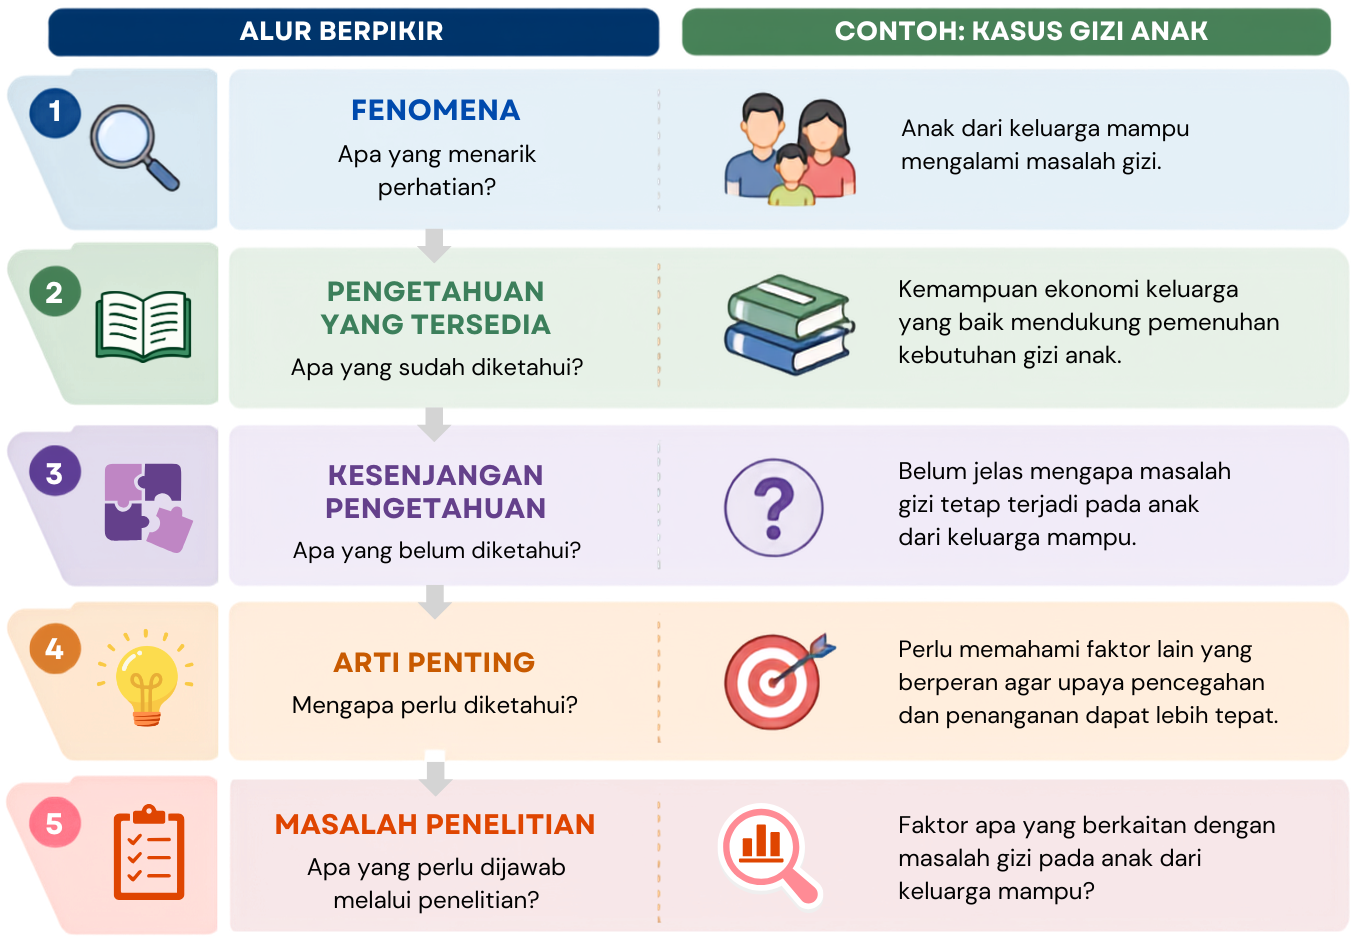
\includegraphics[keepaspectratio]{images/fenomena.png}}

}

\caption{\label{fig-fenomena}Dari Fenomena Menjadi Masalah Penelitian}

\end{figure}%

\section{Mengidentifikasi Kesenjangan
Pengetahuan}\label{mengidentifikasi-kesenjangan-pengetahuan}

\emph{Research gap} menunjukkan adanya pengetahuan atau bukti yang belum
memadai untuk menjawab suatu persoalan penelitian. Kesenjangan tersebut
tidak selalu berarti bahwa suatu topik sama sekali belum pernah
diteliti. Kesenjangan juga dapat muncul karena bukti yang tersedia belum
konsisten, teori belum memberikan penjelasan yang memadai, metode
penelitian sebelumnya memiliki keterbatasan, atau pengetahuan yang
tersedia belum mencakup konteks tertentu. Kesenjangan penelitian dapat
diklasifikasikan dengan berbagai cara (Robinson dkk., 2011). Untuk
memudahkan pemahaman, kesenjangan pengetahuan dalam bab ini
dikelompokkan ke dalam empat bentuk berikut:

\begin{enumerate}
\def\labelenumi{\arabic{enumi}.}
\item
  \textbf{Kesenjangan empiris}

  Kesenjangan ini muncul ketika pengetahuan yang tersedia belum cukup
  untuk memberikan jawaban yang meyakinkan. Hal ini dapat terjadi karena
  suatu aspek belum banyak diketahui, bukti yang tersedia masih
  terbatas, atau penelitian-penelitian sebelumnya menghasilkan temuan
  yang tidak konsisten (Müller-Bloch \& Kranz, 2015).

  Sebagai contoh, suatu penelitian menemukan bahwa dukungan pasangan
  berkaitan dengan \emph{work-family conflict} pada perempuan menikah
  yang bekerja, sedangkan penelitian lain tidak menemukan hubungan
  tersebut. Sebelum menjadikannya dasar penelitian baru, peneliti perlu
  memeriksa apakah perbedaan tersebut berkaitan dengan karakteristik
  partisipan, konteks, pengukuran, desain, atau metode analisis.
\item
  \textbf{Kesenjangan teoretis}

  Kesenjangan teoretis muncul ketika teori yang tersedia belum mampu
  menjelaskan suatu fenomena secara memadai atau ketika beberapa
  perspektif teoretis memberikan penjelasan yang berbeda mengenai
  fenomena yang sama.

  Sebagai contoh, \emph{work/family border theory} menjelaskan bahwa
  fleksibilitas kerja dapat mengaburkan batas antara kehidupan pekerjaan
  dan pribadi sehingga berpotensi menimbulkan konflik peran (Clark,
  2000). Sementara itu, \emph{job demands-resources theory} memandang
  fleksibilitas sebagai sumber daya yang dapat meningkatkan kontrol
  karyawan terhadap pekerjaannya dan mendukung kesejahteraan (Bakker \&
  Demerouti, 2007). Perbedaan penjelasan tersebut membuka ruang untuk
  meneliti kondisi yang membuat fleksibilitas kerja dapat memberikan
  konsekuensi yang berbeda bagi karyawan.
\item
  \textbf{Kesenjangan metodologis}

  Kesenjangan metodologis muncul ketika pengetahuan mengenai suatu
  fenomena masih dibatasi oleh metode yang digunakan dalam penelitian
  sebelumnya (Müller-Bloch \& Kranz, 2015). Keterbatasan tersebut dapat
  berkaitan dengan desain penelitian, teknik pengumpulan data,
  karakteristik sampel, maupun cara suatu variabel diukur.

  Sebagai contoh, penelitian mengenai hubungan penggunaan media sosial
  dan kesejahteraan psikologis mungkin sebagian besar menggunakan desain
  \emph{cross-sectional}, yaitu mengukur kedua variabel pada satu waktu.
  Desain tersebut dapat menunjukkan hubungan antar variabel, tetapi
  belum dapat menggambarkan bagaimana perubahan keduanya berlangsung
  dari waktu ke waktu. Penggunaan desain longitudinal pada penelitian
  berikutnya dapat membantu mengisi keterbatasan metodologis tersebut.
\item
  \textbf{Kesenjangan praktis}

  Kesenjangan praktis muncul ketika terdapat sesuatu yang diperlukan
  untuk memahami, mengukur, atau menangani suatu persoalan, tetapi
  pengetahuan, metode, instrumen, atau sumber daya yang tersedia belum
  memadai untuk memenuhi kebutuhan tersebut. Kesenjangan ini dapat
  ditemukan dalam praktik di masyarakat maupun dalam kegiatan akademik
  dan penelitian.

  Sebagai contoh, \emph{Psychological Well-Being Scale} yang
  dikembangkan oleh Ryff \& Keyes (1995) telah banyak digunakan dan
  diadaptasi dalam berbagai konteks budaya, termasuk Indonesia. Namun,
  beberapa indikator pada aspek \emph{autonomy} dapat menunjukkan
  karakteristik psikometris yang kurang memadai ketika digunakan dalam
  konteks Indonesia. Jika indikator yang tersedia belum mampu mengukur
  \emph{autonomy} secara memadai, terdapat kebutuhan untuk
  mengidentifikasi indikator yang lebih sesuai dengan bagaimana
  kemandirian dipahami dan diwujudkan dalam konteks budaya Indonesia.
\end{enumerate}

Keempat bentuk kesenjangan tersebut tidak selalu berdiri sendiri dan
satu masalah dapat melibatkan lebih dari satu jenis kesenjangan. Karena
itu, tujuan mengidentifikasi kesenjangan bukan sekadar menentukan
jenisnya, tetapi menunjukkan \textbf{apa yang belum diketahui, mengapa
pengetahuan yang tersedia belum memadai, dan mengapa penelitian baru
diperlukan}.

Peneliti juga perlu berhati-hati menggunakan pernyataan \textbf{``belum
pernah diteliti''} sebagai dasar penelitian. Belum adanya penelitian
pada suatu lokasi atau kelompok tertentu tidak dengan sendirinya
menunjukkan kesenjangan pengetahuan yang bermakna. Peneliti perlu
menjelaskan mengapa karakteristik konteks atau kelompok tersebut secara
konseptual penting dan bagaimana penelitian pada konteks tersebut dapat
menambah, menguji, atau memperbaiki pengetahuan yang sudah tersedia.

\section{Menemukan Masalah
Penelitian}\label{menemukan-masalah-penelitian}

Ide penelitian dapat muncul dari berbagai sumber, bahkan dari pengamatan
atau gagasan awal yang masih samar. Tugas peneliti adalah mengembangkan
gagasan tersebut menjadi masalah yang jelas dan dapat diteliti secara
ilmiah (Kerlinger \& Lee, 2000). Beberapa sumber yang dapat digunakan
untuk menemukan masalah penelitian antara lain:

\begin{enumerate}
\def\labelenumi{\arabic{enumi}.}
\tightlist
\item
  \textbf{Observasi dan data awal.} Fenomena atau kejanggalan yang
  ditemukan dalam kehidupan sehari-hari dapat memunculkan pertanyaan
  yang layak diteliti. Data dari lembaga pemerintah, organisasi, atau
  sumber dokumentasi lainnya juga dapat menunjukkan persoalan yang
  membutuhkan penjelasan lebih lanjut.
\item
  \textbf{Literatur ilmiah.} Buku dan terutama artikel jurnal membantu
  peneliti mengetahui perkembangan suatu topik sekaligus menemukan
  hal-hal yang belum terjawab. Misalnya, penelitian yang satu menemukan
  hubungan antara dukungan pasangan dan \emph{work-family conflict},
  sedangkan penelitian lain tidak menemukannya. Perbedaan tersebut dapat
  menjadi titik awal untuk mengidentifikasi masalah penelitian.
\item
  \textbf{Forum ilmiah.} Seminar, konferensi, lokakarya, dan diskusi
  akademik mempertemukan peneliti dengan perkembangan teori, metode, dan
  temuan terbaru. Karena itu, forum ilmiah dapat membantu menemukan
  persoalan yang relevan dan aktual.
\item
  \textbf{Penelitian terdahulu.} Penelitian sebelumnya dapat memunculkan
  masalah baru melalui replikasi, perluasan, atau perbaikan terhadap
  keterbatasan penelitian. Rekomendasi penelitian selanjutnya juga dapat
  menjadi petunjuk, tetapi tetap perlu ditelaah secara kritis untuk
  memastikan bahwa persoalan tersebut masih relevan.
\end{enumerate}

Berbagai sumber tersebut pada dasarnya membantu peneliti menemukan
\textbf{kesenjangan antara pengetahuan yang sudah tersedia dan
pengetahuan yang masih diperlukan}. Karena itu, menemukan masalah
penelitian bukan sekadar mencari topik yang menarik, tetapi merupakan
proses membaca, mengamati, membandingkan bukti, dan mempertanyakan
hal-hal yang belum memperoleh jawaban memadai (Kumar, 2018).

\section{Menilai Kelayakan Masalah
Penelitian}\label{menilai-kelayakan-masalah-penelitian}

Menemukan kesenjangan pengetahuan belum berarti bahwa masalah tersebut
layak untuk diteliti. Peneliti juga perlu mempertimbangkan apakah
penelitian dapat dilaksanakan, memberikan kontribusi, dan memenuhi
prinsip etika. Salah satu kerangka yang dapat digunakan untuk menilainya
adalah \textbf{\emph{FINE}}, yaitu \emph{Feasible, Interesting, Novel,}
dan \emph{Ethical} (Browner dkk., 2023).

\begin{enumerate}
\def\labelenumi{\arabic{enumi}.}
\tightlist
\item
  \textbf{\emph{Feasible}} \textbf{(dapat dilaksanakan).} Penelitian
  harus realistis untuk dilakukan dengan sumber daya yang tersedia.
  Peneliti perlu mempertimbangkan ketersediaan dan jumlah partisipan
  atau data, kompetensi yang diperlukan, waktu, biaya, fasilitas, serta
  ruang lingkup penelitian. Jika penelitian terlalu luas atau
  membutuhkan sumber daya yang tidak tersedia, pertanyaan penelitian
  perlu dipersempit atau desainnya disesuaikan.
\item
  \textbf{\emph{Important}} \textbf{(penting).} Penelitian sebaiknya
  menjawab persoalan yang memiliki arti bagi pengembangan pengetahuan
  atau kesejahteraan manusia. Peneliti perlu mempertimbangkan apakah
  hasil penelitian berpotensi memperluas pengetahuan ilmiah, memengaruhi
  praktik atau kebijakan, maupun memberikan arah bagi penelitian
  selanjutnya. Dengan demikian, pentingnya suatu masalah tidak hanya
  ditentukan oleh ketertarikan peneliti, tetapi juga oleh kontribusi
  yang mungkin dihasilkan.
\item
  \textbf{\emph{Novel}} \textbf{(memiliki kebaruan).} Penelitian perlu
  memberikan tambahan yang bermakna terhadap pengetahuan yang telah
  tersedia. Kebaruan tidak berarti bahwa topik harus sama sekali belum
  pernah diteliti. Penelitian dapat bernilai baru apabila mereplikasi
  temuan penting, menguji apakah temuan berlaku pada populasi lain,
  memperbaiki kelemahan penelitian sebelumnya, atau menggunakan metode
  baru untuk memperjelas pengetahuan yang telah ada.
\item
  \textbf{\emph{Ethical}} \textbf{(etis).} Pertanyaan penelitian harus
  dapat dijawab melalui penelitian yang menghormati hak, keselamatan,
  privasi, dan kesejahteraan partisipan. Peneliti juga perlu
  mempertimbangkan aspek keadilan, termasuk memastikan bahwa penelitian
  tidak memperbesar ketimpangan dan, sejauh relevan, melibatkan kelompok
  dengan latar belakang dan pengalaman yang beragam.
\end{enumerate}

Keempat kriteria tersebut perlu dipertimbangkan secara bersama-sama.
Masalah yang penting dan memiliki kebaruan belum tentu layak diteliti
apabila tidak dapat dilaksanakan atau menimbulkan persoalan etis.
\textbf{Kerangka \emph{FINE} membantu peneliti memilih masalah yang
penting dan memberikan kontribusi, sekaligus realistis dan etis untuk
diteliti.}

\section{Merumuskan Masalah
Penelitian}\label{merumuskan-masalah-penelitian}

Setelah masalah yang layak diteliti ditemukan, langkah berikutnya adalah
merumuskannya secara jelas. \textbf{Rumusan masalah merupakan uraian
argumentatif mengenai persoalan yang hendak diteliti, kesenjangan
pengetahuan yang mendasarinya, serta alasan mengapa persoalan tersebut
perlu diteliti.} Rumusan masalah yang jelas akan membantu mengarahkan
berbagai keputusan berikutnya dalam proses penelitian (Kumar, 2018).

Secara umum, rumusan masalah yang baik memuat empat komponen berikut:

\begin{enumerate}
\def\labelenumi{\arabic{enumi}.}
\tightlist
\item
  \textbf{Fenomena atau persoalan yang menjadi perhatian.} Peneliti
  menjelaskan kondisi atau gejala yang melatarbelakangi munculnya
  masalah penelitian.
\item
  \textbf{Kesenjangan pengetahuan.} Peneliti menunjukkan apa yang belum
  diketahui atau belum dapat dijelaskan secara memadai berdasarkan
  pengetahuan yang tersedia.
\item
  \textbf{\emph{Rationale}} \textbf{atau arti penting masalah.} Peneliti
  menjelaskan mengapa kesenjangan tersebut penting untuk diteliti dan
  apa kontribusi yang dapat diperoleh dengan menjawabnya.
\item
  \textbf{Arah penelitian.} Peneliti menunjukkan aspek, variabel, atau
  hubungan yang perlu diteliti untuk mengisi kesenjangan tersebut.
\end{enumerate}

Sebagai contoh, perempuan dewasa awal yang mengalami perlakuan buruk
dalam hubungan romantis terkadang tetap sulit meninggalkan pasangannya.
Salah satu kondisi yang diduga berkaitan dengan keadaan tersebut adalah
\emph{emotional dependency}. Sementara itu, kondisi \emph{fatherless}
diperkirakan berkaitan dengan perkembangan emosional dan hubungan
interpersonal. Namun, bukti mengenai hubungan antara \emph{fatherless}
dan \emph{emotional dependency} pada perempuan dewasa awal masih
terbatas. Oleh karena itu, diperlukan penelitian mengenai keterkaitan
kedua variabel tersebut.

Berdasarkan uraian tersebut, masalah penelitian dapat dirumuskan dalam
bentuk pertanyaan:

\begin{quote}
\textbf{``Apakah terdapat hubungan antara kondisi \emph{fatherless} dan
\emph{emotional dependency} dalam hubungan romantis pada perempuan
dewasa awal?''}
\end{quote}

Contoh tersebut menunjukkan bahwa perumusan masalah tidak dimulai dengan
membuat kalimat tanya. Peneliti terlebih dahulu membangun argumentasi
mengenai fenomena yang diamati, kesenjangan pengetahuan, arti penting
masalah, dan arah penelitian. Rumusan tersebut kemudian dapat dinyatakan
dalam bentuk pertanyaan yang sekaligus berfungsi sebagai pertanyaan
penelitian.

\section{Merumuskan Pertanyaan
Penelitian}\label{merumuskan-pertanyaan-penelitian}

Pertanyaan penelitian menyatakan secara spesifik \textbf{apa yang hendak
diketahui melalui penelitian}. Dalam banyak penelitian,
\textbf{pertanyaan ini sekaligus menjadi bentuk akhir dari rumusan
masalah.} Pertanyaan penelitian menjadi acuan dalam menentukan data yang
perlu dikumpulkan dan cara data tersebut dianalisis (Kumar, 2018).

\subsection{Karakteristik Pertanyaan Penelitian yang
Baik}\label{karakteristik-pertanyaan-penelitian-yang-baik}

Kerlinger \& Lee (2000) menekankan bahwa masalah atau pertanyaan ilmiah
perlu dinyatakan secara jelas, menunjukkan hubungan antar variabel
ketika hubungan tersebut memang menjadi fokus penelitian, serta
memungkinkan pengujian secara empiris. Secara lebih umum, pertanyaan
penelitian yang baik memiliki karakteristik berikut:

\begin{enumerate}
\def\labelenumi{\arabic{enumi}.}
\tightlist
\item
  \textbf{Jelas dan spesifik}, sehingga tidak menimbulkan penafsiran
  yang berbeda mengenai apa yang hendak diketahui.
\item
  \textbf{Dapat dijawab secara empiris}, yaitu jawabannya dapat
  diperoleh melalui pengumpulan dan analisis data.
\item
  \textbf{Menunjukkan variabel atau fenomena yang diteliti}, serta
  hubungan atau perbandingan antar variabel apabila memang menjadi fokus
  penelitian.
\item
  \textbf{Menunjukkan populasi atau konteks penelitian apabila
  diperlukan}, sehingga ruang lingkup pertanyaan menjadi jelas.
\item
  \textbf{Selaras dengan masalah penelitian}, sehingga jawaban terhadap
  pertanyaan tersebut benar-benar membantu mengisi kesenjangan
  pengetahuan yang telah diidentifikasi.
\end{enumerate}

Pertanyaan juga perlu dirumuskan sesuai dengan \textbf{jenis bukti yang
dapat dihasilkan oleh penelitian}. Misalnya, penelitian yang hanya
mengukur hubungan antara dua variabel tidak seharusnya merumuskan
pertanyaan yang menuntut kesimpulan sebab-akibat.

\subsection{Jenis Pertanyaan
Penelitian}\label{jenis-pertanyaan-penelitian}

Dalam penelitian kuantitatif, pertanyaan penelitian dapat dibedakan
berdasarkan jenis informasi yang hendak diperoleh.

\begin{enumerate}
\def\labelenumi{\arabic{enumi}.}
\item
  \textbf{Deskriptif}

  Pertanyaan deskriptif bertujuan menggambarkan keadaan atau
  karakteristik suatu variabel pada populasi tertentu.

  \begin{quote}
  \emph{Bagaimana gambaran resiliensi Generasi Z yang tinggal di daerah
  yang pernah mengalami bencana alam?}
  \end{quote}
\item
  \textbf{Komparatif}

  Pertanyaan komparatif bertujuan mengetahui apakah terdapat perbedaan
  suatu variabel antara dua kelompok atau lebih.

  \begin{quote}
  \emph{Apakah terdapat perbedaan tingkat resiliensi antara Generasi Z
  yang tinggal di daerah yang pernah mengalami bencana alam dan yang
  tinggal di daerah yang tidak pernah mengalaminya?}
  \end{quote}
\item
  \textbf{Asosiatif}

  Pertanyaan asosiatif bertujuan mengetahui apakah dua atau lebih
  variabel saling berhubungan, tanpa dengan sendirinya menyatakan bahwa
  salah satu variabel menyebabkan variabel lainnya.

  \begin{quote}
  \emph{Apakah pengalaman menghadapi bencana berkaitan dengan tingkat
  resiliensi pada Generasi Z?}
  \end{quote}
\item
  \textbf{Kausal}

  Pertanyaan kausal bertujuan mengetahui apakah perubahan pada suatu
  variabel menyebabkan perubahan pada variabel lainnya. Karena
  mengandung klaim sebab-akibat, pertanyaan semacam ini memerlukan
  desain penelitian yang memungkinkan peneliti memperoleh bukti mengenai
  hubungan kausal.

  \begin{quote}
  \emph{Apakah pemberian pelatihan kesiapsiagaan bencana meningkatkan
  resiliensi pada Generasi Z?}
  \end{quote}
\end{enumerate}

Pemilihan kata dalam pertanyaan penelitian perlu diperhatikan karena
menunjukkan jenis kesimpulan yang hendak diperoleh. Istilah seperti
\textbf{``berhubungan''} atau \textbf{``berkaitan''} menunjukkan
pertanyaan asosiatif, sedangkan \textbf{``menyebabkan'',
``memengaruhi'', ``meningkatkan'',} atau \textbf{``menurunkan''}
mengandung makna kausal. Perbedaan ini penting karena jenis pertanyaan
penelitian akan berhubungan dengan desain penelitian yang diperlukan
untuk menjawabnya.

\section{Pertanyaan Penelitian dan Desain
Penelitian}\label{pertanyaan-penelitian-dan-desain-penelitian}

Pertanyaan penelitian berkaitan dengan desain yang digunakan untuk
menjawabnya. Pertanyaan deskriptif bertujuan menggambarkan suatu
fenomena, pertanyaan komparatif membandingkan kelompok atau kondisi,
sedangkan pertanyaan asosiatif menguji hubungan antarvariabel. Sementara
itu, pertanyaan kausal membutuhkan bukti yang lebih kuat karena
bertujuan menunjukkan bahwa perubahan pada satu variabel menyebabkan
perubahan pada variabel lainnya.

Hubungan statistik antara dua variabel saja belum cukup untuk
menunjukkan hubungan sebab-akibat. Misalnya, hubungan antara
\textbf{bermain gim yang mengandung kekerasan} dan \textbf{agresivitas
anak} tidak serta-merta menunjukkan bahwa bermain gim menyebabkan
agresivitas. Hubungan tersebut mungkin dipengaruhi oleh variabel lain,
seperti pola asuh orang tua (\emph{third-variable problem}). Selain itu,
arah hubungan juga dapat dipertanyakan: bermain gim mungkin memengaruhi
agresivitas, tetapi anak yang lebih agresif juga mungkin lebih tertarik
pada gim yang mengandung kekerasan (\emph{directionality problem}).

Oleh karena itu, \textbf{pertanyaan penelitian harus dirumuskan sesuai
dengan jenis bukti yang dapat dihasilkan oleh desain penelitian}. Studi
korelasional lebih tepat digunakan untuk menjawab apakah variabel
\emph{berhubungan} atau \emph{berkaitan}, bukan untuk menyimpulkan
hubungan sebab-akibat (Shadish dkk., 2002). Pembahasan lebih lanjut
mengenai hal ini akan disampaikan pada Bab~\ref{sec-desain}.

\section{Contoh Terintegrasi: Dari Fenomena ke Pertanyaan
Penelitian}\label{contoh-terintegrasi-dari-fenomena-ke-pertanyaan-penelitian}

Proses merumuskan masalah dan pertanyaan penelitian tidak berlangsung
sebagai tahapan yang sepenuhnya terpisah. Peneliti bergerak dari
fenomena yang diamati, menelaah pengetahuan yang tersedia, menemukan
kesenjangan, lalu mengerucutkannya menjadi masalah dan pertanyaan
penelitian. Contoh pada Tabel~\ref{tbl-contoh} menggambarkan proses
tersebut.

\begin{longtable}[]{@{}
  >{\raggedright\arraybackslash}p{(\linewidth - 2\tabcolsep) * \real{0.3611}}
  >{\raggedright\arraybackslash}p{(\linewidth - 2\tabcolsep) * \real{0.6389}}@{}}
\caption{Contoh Tahapan dari Fenomena hingga Penentuan Desain
Penelitian}\label{tbl-contoh}\tabularnewline
\toprule\noalign{}
\endfirsthead
\endhead
\bottomrule\noalign{}
\endlastfoot
\textbf{Tahap} & \textbf{Uraian} \\
\textbf{Topik} & Fleksibilitas kerja dan kesejahteraan karyawan \\
\textbf{Fenomena} & Kebijakan \emph{work from anywhere} (WFA) memberikan
fleksibilitas kepada karyawan, tetapi sebagian karyawan justru mengalami
kesulitan membatasi waktu kerja dan kehidupan pribadi. \\
\textbf{Pengetahuan yang tersedia} & \emph{Work/family border theory}
menjelaskan bahwa fleksibilitas dapat mengaburkan batas pekerjaan dan
kehidupan pribadi (Clark, 2000). Sebaliknya, \emph{job demands-resources
theory} memandang fleksibilitas sebagai sumber daya yang dapat membantu
karyawan mengelola tuntutan pekerjaan (Bakker \& Demerouti, 2007). \\
\textbf{Kesenjangan pengetahuan} & Kedua perspektif tersebut membuka
pertanyaan mengenai kondisi ketika fleksibilitas kerja mendukung atau
justru menghambat kesejahteraan karyawan. \\
\textbf{Masalah penelitian} & Bagaimana fleksibilitas kerja berkaitan
dengan kesejahteraan psikologis karyawan? \\
\textbf{Pertanyaan penelitian} & Apakah terdapat hubungan antara
fleksibilitas kerja dan \emph{psychological well-being} pada
karyawan? \\
\textbf{Implikasi desain} & Pertanyaan tersebut bersifat asosiatif
sehingga dapat dijawab melalui penelitian korelasional dengan mengukur
fleksibilitas kerja dan \emph{psychological well-being}. \\
\end{longtable}

Contoh tersebut menunjukkan bahwa pertanyaan penelitian dikembangkan
melalui proses yang berangkat dari fenomena, pengetahuan yang tersedia,
dan kesenjangan pengetahuan.

\begin{tcolorbox}[enhanced jigsaw, colframe=quarto-callout-tip-color-frame, toptitle=1mm, breakable, leftrule=.75mm, arc=.35mm, toprule=.15mm, colback=white, colbacktitle=quarto-callout-tip-color!10!white, bottomtitle=1mm, bottomrule=.15mm, titlerule=0mm, title=\textcolor{quarto-callout-tip-color}{\faLightbulb}\hspace{0.5em}{Rangkuman}, coltitle=black, left=2mm, opacitybacktitle=0.6, opacityback=0, rightrule=.15mm]

\begin{enumerate}
\def\labelenumi{\arabic{enumi}.}
\tightlist
\item
  Penelitian berawal dari masalah yang membutuhkan jawaban, bukan
  sekadar dari topik atau fenomena yang menarik.
\item
  Masalah penelitian muncul ketika terdapat kesenjangan antara
  pengetahuan yang telah tersedia dan sesuatu yang masih perlu diketahui
  atau dijelaskan.
\item
  Kesenjangan pengetahuan dapat berkaitan dengan bukti empiris, teori,
  metode, maupun kebutuhan praktis.
\item
  Masalah penelitian dapat ditemukan melalui observasi dan data awal,
  literatur ilmiah, forum ilmiah, serta penelitian terdahulu, kemudian
  dinilai kelayakannya menggunakan kriteria FINER: \emph{Feasible,
  Interesting, Novel, Ethical,} dan \emph{Relevant}.
\item
  Rumusan masalah dibangun dengan memperhatikan fenomena, kesenjangan
  pengetahuan, arti penting masalah, dan arah penelitian, kemudian
  dikerucutkan menjadi pertanyaan yang dapat dijawab secara empiris.
\item
  Pertanyaan penelitian dapat bersifat deskriptif, komparatif,
  asosiatif, atau kausal. Jenis pertanyaan harus selaras dengan desain
  penelitian dan jenis bukti yang dapat dihasilkan.
\end{enumerate}

\end{tcolorbox}

\begin{tcolorbox}[enhanced jigsaw, colframe=quarto-callout-important-color-frame, toptitle=1mm, breakable, leftrule=.75mm, arc=.35mm, toprule=.15mm, colback=white, colbacktitle=quarto-callout-important-color!10!white, bottomtitle=1mm, bottomrule=.15mm, titlerule=0mm, title=\textcolor{quarto-callout-important-color}{\faExclamation}\hspace{0.5em}{Refleksi \& Diskusi}, coltitle=black, left=2mm, opacitybacktitle=0.6, opacityback=0, rightrule=.15mm]

\begin{itemize}
\tightlist
\item
  Perhatikan sebuah fenomena yang sedang menarik perhatian Anda. Apa
  yang membuat fenomena tersebut belum dapat langsung disebut sebagai
  masalah penelitian? Informasi apa yang perlu Anda ketahui terlebih
  dahulu?
\item
  Pernyataan \emph{``topik ini belum pernah diteliti pada mahasiswa
  Universitas X''} sering digunakan sebagai alasan melakukan penelitian.
  Apakah pernyataan tersebut sudah cukup menunjukkan adanya
  \emph{research gap}? Jelaskan alasan Anda.
\item
  Seorang mahasiswa menemukan bahwa beberapa penelitian menunjukkan
  penggunaan media sosial berkaitan dengan kesejahteraan psikologis yang
  lebih rendah, sedangkan penelitian lainnya tidak menemukan hubungan
  tersebut. Jenis kesenjangan apa yang mungkin ditemukan? Apa yang perlu
  diperiksa sebelum mahasiswa memutuskan melakukan penelitian baru?
\item
  Perhatikan pertanyaan berikut: ``Apakah penggunaan gim yang mengandung
  kekerasan menyebabkan agresivitas pada remaja?'' Jika peneliti hanya
  merencanakan survei korelasional satu kali pengukuran, apa yang perlu
  diperbaiki dari pertanyaan tersebut dan mengapa?
\item
  Pilih satu topik penelitian yang Anda minati. Susun secara berurutan:
  fenomena → pengetahuan yang tersedia → kesenjangan pengetahuan →
  masalah penelitian → satu pertanyaan penelitian. Kemudian tentukan
  apakah pertanyaan tersebut bersifat deskriptif, komparatif, asosiatif,
  atau kausal.
\end{itemize}

\end{tcolorbox}

\section*{Daftar Pustaka}\label{daftar-pustaka}

\markright{Daftar Pustaka}

\phantomsection\label{refs--3}
\begin{CSLReferences}{1}{0}
\bibitem[\citeproctext]{ref-Bakker2007--3}
Bakker, A. B., \& Demerouti, E. (2007). The Job Demands‐Resources model:
state of the art. \emph{Journal of Managerial Psychology}, \emph{22},
309--328. \url{https://doi.org/10.1108/02683940710733115}

\bibitem[\citeproctext]{ref-Browner2023--3}
Browner, W. S., Newman, T. B., Cummings, S. R., Grady, D., Huang, A. J.,
Kanaya, A. M., \& Pletcher, M. (2023). \emph{Designing clinical
research} (4th ed.). Lippincott Williams \& Wilkins.

\bibitem[\citeproctext]{ref-Clark2000--3}
Clark, S. C. (2000). Work/Family Border Theory: A New Theory of
Work/Family Balance. \emph{Human Relations}, \emph{53}, 747--770.
\url{https://doi.org/10.1177/0018726700536001}

\bibitem[\citeproctext]{ref-Kerlinger2000--3}
Kerlinger, F. N., \& Lee, H. B. (2000). \emph{Foundations of behavioral
research} (4th ed.). Harcourt College Publishers.

\bibitem[\citeproctext]{ref-Kumar2018--3}
Kumar, R. (2018). \emph{Research Methodology: A Step-by-Step Guide for
Beginners} (3rd ed.). Sage Publications.

\bibitem[\citeproctext]{ref-Mller-Bloch2015--3}
Müller-Bloch, C., \& Kranz, J. (2015). A Framework for Rigorously
Identifying Research Gaps in Qualitative Literature Reviews. \emph{2015
international conference on information systems: Exploring the
information frontier, ICIS 2015}, 1--19.

\bibitem[\citeproctext]{ref-Robinson2011--3}
Robinson, K. A., Saldanha, I. J., \& Mckoy, N. A. (2011). Development of
a framework to identify research gaps from systematic reviews.
\emph{Journal of Clinical Epidemiology}, \emph{64}, 1325--1330.
\url{https://doi.org/10.1016/j.jclinepi.2011.06.009}

\bibitem[\citeproctext]{ref-Ryff1995--3}
Ryff, C. D., \& Keyes, C. L. M. (1995). The structure of psychological
well-being revisited. \emph{Journal of Personality and Social
Psychology}, \emph{69}, 719--727.
\url{https://doi.org/10.1037/0022-3514.69.4.719}

\bibitem[\citeproctext]{ref-Shadish2002--3}
Shadish, W. R., Cook, T. D., \& Campbell, D. T. (2002).
\emph{Experimental and quasi-experimental designs for generalized causal
inference} (2nd ed.). Wadsworth/Cengage Learning.

\end{CSLReferences}

\chapter{Tinjauan Literatur dan Pengembangan Kerangka
Teoretis}\label{tinjauan-literatur-dan-pengembangan-kerangka-teoretis}

\begin{tcolorbox}[enhanced jigsaw, colframe=quarto-callout-note-color-frame, toptitle=1mm, breakable, leftrule=.75mm, arc=.35mm, toprule=.15mm, colback=white, colbacktitle=quarto-callout-note-color!10!white, bottomtitle=1mm, bottomrule=.15mm, titlerule=0mm, title=\textcolor{quarto-callout-note-color}{\faInfo}\hspace{0.5em}{Capaian Pembelajaran}, coltitle=black, left=2mm, opacitybacktitle=0.6, opacityback=0, rightrule=.15mm]

Setelah mempelajari bab ini, mahasiswa diharapkan mampu:

\begin{enumerate}
\def\labelenumi{\arabic{enumi}.}
\tightlist
\item
  Menjelaskan pengertian tinjauan literatur serta perannya dalam proses
  penelitian ilmiah.
\item
  Menjelaskan tujuan tinjauan literatur dalam membangun landasan
  teoretis penelitian.
\item
  Mengidentifikasi berbagai jenis sumber literatur ilmiah yang relevan
  dengan topik penelitian.
\item
  Menilai kualitas sumber pustaka berdasarkan relevansi, kemutakhiran,
  dan kredibilitas ilmiahnya.
\item
  Menggunakan strategi penelusuran literatur secara sistematis, seperti
  backward referencing dan forward referencing.
\item
  Memahami prinsip etika akademik dalam penggunaan sumber literatur dan
  penulisan kutipan.
\item
  Mengintegrasikan teori dan temuan penelitian sebelumnya dalam suatu
  kerangka teoretis.
\item
  Mengembangkan model konseptual penelitian yang menjelaskan hubungan
  antar variabel.
\end{enumerate}

\end{tcolorbox}

\section{Pengertian Tinjauan
Literatur}\label{pengertian-tinjauan-literatur}

Setiap penelitian ilmiah tidak pernah dimulai dari ruang kosong.
Sebaliknya, penelitian selalu dibangun di atas pengetahuan, gagasa, dan
temuan yang telah dikembangkan oleh para peneliti sebelumnya. Oleh
karena itu, salah satu tahap penting dalam proses penelitian adalah
melakukan tinjauan literatur atau tinjauan pustaka.

Tinjauan literatur merupakan proses sistematis untuk mengidentifikasi,
mengevaluasi, dan mensintesis berbagai sumber ilmiah yang relevan dengan
topik penelitian. Melalui proses ini, peneliti dapat memahami
perkembangan teori, temuan empiris, serta pendekatan metodologis yang
telah digunakan dalam penelitian sebelumnya.

Secara umum, tujuan utama tinjauan literatur adalah untuk menemukan
konsep, teori, atau generalisasi yang dapat dijadikan landasan teoretis
bagi penelitian yang akan dilakukan. Selain itu, tinjauan literatur juga
membantu peneliti menemukan metode penelitian yang tepat serta
memperluas pemahaman mengenai fenomena yang diteliti.

Menurut Creswell \& Clark (2018), tinjauan literatur memiliki beberapa
fungsi penting dalam penelitian, antara lain:

\begin{enumerate}
\def\labelenumi{\arabic{enumi}.}
\tightlist
\item
  Menunjukkan bahwa peneliti memahami perkembangan pengetahuan pada
  bidang yang diteliti.
\item
  Mengidentifikasi kesenjangan penelitian (\emph{research gap}).
\item
  Memberikan dasar konseptual bagi pengembangan hipotesis atau
  pertanyaan penelitian.
\item
  Menjelaskan bagaimana penelitian yang dilakukan berkontribusi pada
  pengembangan ilmu pengetahuan.
\end{enumerate}

Dengan demikian, tinjauan literatur tidak sekadar menjadi kumpulan
ringkasan penelitian terdahulu, tetapi merupakan analisis kritis yang
membantu membangun kerangka berpikir penelitian.

\section{Tujuan Tinjauan Literatur dalam
Penelitian}\label{tujuan-tinjauan-literatur-dalam-penelitian}

Dalam penelitian ilmiah, tinjauan literatur memiliki beberapa tujuan
utama, yaitu:

\begin{enumerate}
\def\labelenumi{\arabic{enumi}.}
\item
  Menyusun landasan teori penelitian

  Penelitian membutuhkan kerangka konseptual yang jelas untuk
  menjelaskan hubungan antar variabel yang diteliti. Melalui tinjauan
  literatur, peneliti dapat menemukan teori-teori yang relevan untuk
  menjelaskan fenomena yang sedang diteliti.

  Sebagai contoh, penelitian mengenai motivasi belajar dapat menggunakan
  teori \emph{self-determination} dari Ryan \& Deci (2000) sebagai
  landasan untuk memahami bagaimana kebutuhan psikologis memengaruhi
  motivasi individu.
\item
  Mengidentifikasi temuan penelitian sebelumnya

  Tinjauan literatur membantu peneliti mengetahui apa saja yang telah
  ditemukan oleh penelitian sebelumnya. Hal ini penting untuk
  menghindari duplikasi penelitian serta membantu peneliti memahami pola
  temuan yang telah ada. Menurut Hart (2025), tinjauan literatur yang
  baik mampu menunjukkan konsistensi maupun perbedaan temuan antar
  penelitian.
\item
  Menentukan pendekatan metodologis yang sesuai

  Selain teori, peneliti juga dapat mempelajari metode yang digunakan
  dalam penelitian sebelumnya. Informasi ini membantu peneliti memilih
  desain penelitian, instrumen pengukuran, dan teknik analisis data yang
  paling tepat.
\item
  Memperluas pemahaman terhadap fenomena penelitian

  Melalui berbagai sumber ilmiah, peneliti dapat memperoleh pemahaman
  yang lebih luas tentang konteks sosial, budaya, maupun psikologis dari
  fenomena yang diteliti.
\end{enumerate}

Dengan demikian, tinjauan literatur berfungsi sebagai fondasi ilmiah
yang memperkuat argumen dan rasionalitas penelitian.

\section{Sumber-sumber Literatur
Ilmiah}\label{sumber-sumber-literatur-ilmiah}

Sumber pustaka dalam penelitian dapat dibedakan menjadi dua kategori
utama, yaitu sumber acuan umum dan sumber acuan khusus.

\begin{enumerate}
\def\labelenumi{\arabic{enumi}.}
\item
  Sumber acuan umum

  Sumber acuan umum biasanya digunakan untuk memahami konsep dasar atau
  teori yang bersifat umum. Contoh sumber acuan umum antara lain:

  \begin{itemize}
  \tightlist
  \item
    Buku teks akademik
  \item
    Ensiklopedia ilmiah
  \item
    \emph{Handbook} dalam bidang ilmu tertentu
  \end{itemize}

  Sumber ini umumnya memberikan gambaran konseptual yang luas mengenai
  suatu topik penelitian.
\item
  Sumber acuan khusus

  Sumber acuan khusus biasanya berisi hasil penelitian yang lebih
  spesifik dan mutakhir. Beberapa contoh sumber acuan khusus antara
  lain:

  \begin{itemize}
  \tightlist
  \item
    Artikel jurnal ilmiah
  \item
    Disertasi atau tesis
  \item
    Laporan penelitian
  \item
    Prosiding konferensi ilmiah
  \item
    Makalah seminar
  \item
    Basis data ilmiah di internet
  \end{itemize}
\end{enumerate}

Dalam penelitian ilmiah, artikel jurnal umumnya dianggap sebagai sumber
referensi yang paling penting karena memuat temuan penelitian terbaru
yang telah melalui proses peer review.

\section{Kriteria Sumber Literatur yang
Baik}\label{kriteria-sumber-literatur-yang-baik}

Tidak semua sumber bacaan dapat dijadikan rujukan dalam penelitian
ilmiah. Oleh karena itu, peneliti perlu mempertimbangkan beberapa
kriteria ketika memilih sumber literatur.

\begin{enumerate}
\def\labelenumi{\arabic{enumi}.}
\item
  Relevansi

  Sumber literatur harus berkaitan langsung dengan topik penelitian yang
  sedang dikaji. Literatur yang tidak relevan hanya akan memperluas
  pembahasan tanpa memberikan kontribusi substantif.
\item
  Kemutakhiran

  Dalam banyak bidang ilmu, terutama psikologi dan ilmu sosial,
  pengetahuan terus berkembang. Oleh karena itu, peneliti dianjurkan
  menggunakan sumber yang relatif mutakhir agar penelitian mencerminkan
  perkembangan terbaru dalam bidang tersebut.
\item
  Kredibilitas ilmiah

  Sumber literatur harus berasal dari publikasi ilmiah yang memiliki
  reputasi baik, seperti jurnal akademik yang terindeks atau penerbit
  akademik yang terpercaya.
\end{enumerate}

Perlu diingat bahwa kualitas penelitian tidak ditentukan oleh banyaknya
jumlah referensi yang digunakan, melainkan oleh relevansi dan kualitas
referensi tersebut.

\section{Strategi Menelusuri
Literatur}\label{strategi-menelusuri-literatur}

Menemukan literatur yang relevan merupakan keterampilan penting bagi
seorang peneliti. Terdapat beberapa strategi yang dapat digunakan untuk
menelusuri literatur ilmiah.

\begin{enumerate}
\def\labelenumi{\arabic{enumi}.}
\item
  \emph{Backward referencing}

  \emph{Backward referencing} dilakukan dengan menelusuri daftar pustaka
  dari artikel atau buku yang dianggap penting. Dengan cara ini,
  peneliti dapat menemukan sumber-sumber yang menjadi dasar bagi
  penelitian tersebut. Strategi ini membantu peneliti memahami
  perkembangan awal suatu konsep atau teori.
\item
  \emph{Forward referencing}

  \emph{Forward referencing} dilakukan dengan mencari artikel-artikel
  yang mengutip suatu karya ilmiah tertentu. Cara ini membantu peneliti
  mengetahui bagaimana suatu teori atau temuan penelitian berkembang
  dari waktu ke waktu. Proses \emph{forward referencing} dapat dilakukan
  melalui berbagai basis data ilmiah seperti Google Scholar atau Scopus.
\end{enumerate}

Kombinasi kedua strategi ini memungkinkan peneliti memperoleh gambaran
yang lebih komprehensif mengenai perkembangan penelitian pada suatu
topik.

\section{Etika Penggunaan Literatur dan
Pengutipan}\label{etika-penggunaan-literatur-dan-pengutipan}

Dalam penulisan karya ilmiah, penggunaan sumber literatur harus
mengikuti prinsip etika akademik. Setiap gagasan, teori, atau data yang
berasal dari sumber lain harus disertai dengan kutipan yang jelas.

Kutipan merupakan cara untuk memberi informasi kepada pembaca bahwa
sebagian gagasan dalam tulisan berasal dari karya ilmiah sebelumnya.
Selain itu, pengutipan juga berfungsi untuk:

\begin{enumerate}
\def\labelenumi{\arabic{enumi}.}
\tightlist
\item
  Menghargai karya ilmiah peneliti lain
\item
  Menunjukkan dasar ilmiah dari argumentasi peneliti
\item
  Memberikan kesempatan kepada pembaca untuk menelusuri sumber asli
\item
  Menjaga integritas dan kejujuran akademik
\end{enumerate}

Dalam psikologi, gaya penulisan kutipan yang paling banyak digunakan
adalah gaya American Psychological Association (APA). Format kutipan
biasanya ditulis dalam bentuk:

\begin{itemize}
\tightlist
\item
  \textbf{Kutipan naratif}: penulis menjadi bagian dari kalimat. Contoh:
  Bandura (1986) menyatakan bahwa pembelajaran sosial terjadi melalui
  proses observasi.
\item
  \textbf{Kutipan dalam tanda kurung}: penulis ditulis dalam kurung.
  Contoh: Pembelajaran sosial dapat terjadi melalui observasi terhadap
  perilaku orang lain (Bandura, 1986).
\end{itemize}

Peneliti harus memastikan bahwa setiap sumber yang dikutip dalam teks
tercantum dalam daftar pustaka.

\section{Pengembangan Kerangka
Teoretis}\label{pengembangan-kerangka-teoretis}

Kerangka teoretis merupakan struktur konseptual yang menjelaskan
hubungan antara konsep atau variabel utama dalam suatu penelitian.
Kerangka ini dibangun berdasarkan teori-teori yang relevan serta temuan
empiris dari penelitian sebelumnya. Dengan demikian, kerangka teoretis
berfungsi sebagai landasan logis yang menjelaskan mengapa suatu variabel
diperkirakan berhubungan dengan variabel lainnya.

Dalam ilmu pengetahuan, teori berperan penting dalam menjelaskan
fenomena yang diamati. Kerlinger \& Lee (2000) mendefinisikan teori
sebagai \emph{``a set of interrelated constructs (concepts),
definitions, and propositions that present a systematic view of
phenomena by specifying relations among variables''}. Definisi ini
menegaskan bahwa teori menyediakan penjelasan sistematis mengenai
hubungan antar variabel yang dapat digunakan untuk memahami dan
memprediksi fenomena tertentu.

Kerangka teoretis dalam penelitian pada dasarnya merupakan penerapan
teori tersebut untuk menjelaskan fenomena yang menjadi fokus penelitian.
Menurut Creswell dan Creswell (2018), kerangka teoretis memberikan dasar
konseptual yang membantu peneliti menjelaskan hubungan antar variabel,
sekaligus menjadi pijakan dalam merumuskan hipotesis penelitian.

Dalam penelitian psikologi, kerangka teoretis memiliki beberapa fungsi
penting.

\begin{enumerate}
\def\labelenumi{\arabic{enumi}.}
\item
  Menjelaskan fenomena penelitian secara konseptual

  Kerangka teoretis membantu peneliti memahami fenomena penelitian
  melalui perspektif teori tertentu. Melalui teori, peneliti dapat
  menjelaskan mekanisme psikologis yang mendasari suatu perilaku atau
  pengalaman manusia.

  Sebagai contoh, penelitian mengenai perilaku prososial sering
  dijelaskan melalui teori empati. Batson (2011) menyatakan bahwa empati
  terhadap penderitaan orang lain dapat memunculkan motivasi altruistik
  untuk membantu individu tersebut. Dengan menggunakan teori tersebut,
  peneliti dapat menjelaskan mengapa empati diperkirakan berhubungan
  dengan perilaku menolong.
\item
  Mengidentifikasi variabel penelitian yang relevan

  Teori juga membantu peneliti menentukan variabel-variabel yang penting
  dalam menjelaskan fenomena yang diteliti. Variabel penelitian biasanya
  berasal dari konsep-konsep yang terdapat dalam teori.

  Misalnya, dalam penelitian mengenai stres kerja, teori \emph{Job
  Demand--Resources Model} menjelaskan bahwa kesejahteraan karyawan
  dipengaruhi oleh tuntutan pekerjaan (\emph{job demands}) dan sumber
  daya pekerjaan (\emph{job resources}). Tuntutan pekerjaan yang tinggi
  dapat meningkatkan stres, sementara sumber daya seperti dukungan
  sosial atau otonomi kerja dapat mengurangi dampak negatif tersebut
  (Bakker \& Demerouti, 2007).

  Dengan merujuk pada teori tersebut, peneliti dapat menentukan
  variabel-variabel penelitian seperti tuntutan kerja, dukungan sosial,
  dan kesejahteraan psikologis.
\item
  Menjelaskan hubungan antar variabel

  Selain membantu menentukan variabel penelitian, teori juga memberikan
  penjelasan mengenai hubungan antar variabel tersebut. Hubungan ini
  tidak hanya didasarkan pada asumsi peneliti, tetapi pada argumentasi
  teoretis yang didukung oleh penelitian sebelumnya.

  Ridley (2012) menyatakan bahwa tinjauan literatur yang baik tidak
  hanya merangkum penelitian sebelumnya, tetapi juga mengintegrasikan
  berbagai temuan tersebut untuk membangun argumen yang logis mengenai
  hubungan antar variabel. Oleh karena itu, kerangka teoretis harus
  mampu menunjukkan bagaimana teori dan penelitian sebelumnya saling
  mendukung dalam menjelaskan fenomena yang diteliti.
\item
  Menjadi dasar bagi pengembangan hipotesis penelitian

  Kerangka teoretis juga menjadi dasar bagi perumusan hipotesis
  penelitian. Hipotesis merupakan pernyataan mengenai hubungan yang
  diperkirakan terjadi antara dua atau lebih variabel yang dapat diuji
  secara empiris.

  Menurut Neuman (2014), hipotesis yang baik harus memiliki dasar
  teoritis yang jelas. Artinya, hubungan antar variabel yang diajukan
  dalam hipotesis harus dapat dijelaskan melalui teori atau temuan
  penelitian sebelumnya.
\end{enumerate}

\begin{tcolorbox}[enhanced jigsaw, colframe=quarto-callout-tip-color-frame, toptitle=1mm, breakable, leftrule=.75mm, arc=.35mm, toprule=.15mm, colback=white, colbacktitle=quarto-callout-tip-color!10!white, bottomtitle=1mm, bottomrule=.15mm, titlerule=0mm, title=\textcolor{quarto-callout-tip-color}{\faLightbulb}\hspace{0.5em}{Rangkuman}, coltitle=black, left=2mm, opacitybacktitle=0.6, opacityback=0, rightrule=.15mm]

\begin{enumerate}
\def\labelenumi{\arabic{enumi}.}
\tightlist
\item
  Tinjauan literatur merupakan proses sistematis untuk menelaah teori,
  konsep, dan temuan penelitian sebelumnya yang relevan dengan topik
  penelitian.
\item
  Tinjauan literatur membantu peneliti memahami perkembangan pengetahuan
  dalam suatu bidang serta mengidentifikasi kesenjangan penelitian.
\item
  Sumber literatur dapat berasal dari berbagai publikasi ilmiah, seperti
  buku teks, artikel jurnal, laporan penelitian, tesis, disertasi, dan
  prosiding konferensi.
\item
  Pemilihan sumber pustaka perlu mempertimbangkan relevansi dengan topik
  penelitian, kemutakhiran sumber, serta kualitas ilmiah publikasi.
\item
  Penelusuran literatur dapat dilakukan melalui berbagai strategi,
  antara lain menelusuri daftar pustaka dari sumber penting
  (\emph{backward referencing}) dan mencari penelitian yang mengutip
  sumber tersebut (\emph{forward referencing}).
\item
  Penggunaan literatur dalam karya ilmiah harus mengikuti prinsip etika
  akademik, termasuk mencantumkan sumber kutipan secara tepat untuk
  menghindari plagiarisme.
\item
  Kerangka teoretis merupakan struktur konseptual yang menjelaskan
  hubungan antar konsep atau variabel dalam penelitian.
\item
  Kerangka teoretis dibangun dengan mengintegrasikan teori dan temuan
  penelitian sebelumnya untuk menjelaskan fenomena yang diteliti.
\item
  Kerangka teoretis menjadi dasar bagi pengembangan model konseptual
  penelitian serta perumusan hipotesis.
\end{enumerate}

\end{tcolorbox}

\begin{tcolorbox}[enhanced jigsaw, colframe=quarto-callout-important-color-frame, toptitle=1mm, breakable, leftrule=.75mm, arc=.35mm, toprule=.15mm, colback=white, colbacktitle=quarto-callout-important-color!10!white, bottomtitle=1mm, bottomrule=.15mm, titlerule=0mm, title=\textcolor{quarto-callout-important-color}{\faExclamation}\hspace{0.5em}{Refleksi \& DIskusi}, coltitle=black, left=2mm, opacitybacktitle=0.6, opacityback=0, rightrule=.15mm]

\begin{itemize}
\tightlist
\item
  Mengapa tinjauan literatur menjadi bagian penting dalam penyusunan
  proposal atau laporan penelitian?
\item
  Apa perbedaan fungsi buku teks dan artikel jurnal ilmiah dalam
  penyusunan tinjauan literatur?
\item
  Bagaimana cara menentukan apakah suatu sumber literatur cukup kredibel
  untuk dijadikan referensi penelitian?
\item
  Mengapa peneliti perlu menggunakan sumber pustaka yang relatif
  mutakhir dalam penelitian ilmiah?
\item
  Bagaimana strategi yang dapat digunakan untuk menemukan literatur yang
  relevan dengan topik penelitian?
\item
  Mengapa pengutipan yang tepat penting dalam menjaga integritas
  akademik dalam penelitian?
\item
  Bagaimana teori membantu peneliti menjelaskan hubungan antar variabel
  dalam suatu penelitian?
\item
  Pilih satu topik penelitian psikologi, lalu diskusikan teori apa saja
  yang dapat digunakan sebagai dasar penyusunan kerangka teoretis
  penelitian tersebut.
\end{itemize}

\end{tcolorbox}

\phantomsection\label{refs--4}
\begin{CSLReferences}{1}{0}
\bibitem[\citeproctext]{ref-Bakker2007--4}
Bakker, A. B., \& Demerouti, E. (2007). The Job Demands‐Resources model:
state of the art. \emph{Journal of Managerial Psychology}, \emph{22},
309--328. \url{https://doi.org/10.1108/02683940710733115}

\bibitem[\citeproctext]{ref-Batson2011--4}
Batson, C. D. (2011). \emph{Altruism in Humans}. Oxford University
Press.

\bibitem[\citeproctext]{ref-Creswell2018--4}
Creswell, J. W., \& Clark, V. L. (2018). \emph{Designing and conducting
mixed methods research} (3rd ed.). SAGE Publications.

\bibitem[\citeproctext]{ref-Hart2025--4}
Hart, C. (2025). \emph{Doing a Literature Review}. SAGE Publications
Ltd. \url{https://doi.org/10.4135/9781036235598}

\bibitem[\citeproctext]{ref-Kerlinger2000--4}
Kerlinger, F. N., \& Lee, H. B. (2000). \emph{Foundations of behavioral
research} (4th ed.). Harcourt College Publishers.

\bibitem[\citeproctext]{ref-Neuman2014--4}
Neuman, W. L. (2014). \emph{Social research methods: Qualitative and
quantitative approaches} (7th ed.). Pearson.

\bibitem[\citeproctext]{ref-Ridley2012--4}
Ridley, D. (2012). \emph{The Literature Review: A Step-By-Step Guide For
Students} (2nd ed.). SAGE Publications Ltd.

\bibitem[\citeproctext]{ref-Ryan2000--4}
Ryan, R. M., \& Deci, E. L. (2000). Self-determination theory and the
facilitation of intrinsic motivation, social development, and
well-being. \emph{American Psychologist}, \emph{55}, 68--78.
\url{https://doi.org/10.1037/0003-066X.55.1.68}

\end{CSLReferences}

\chapter{Desain Penelitian dan Strategi Pengumpulan
Data}\label{sec-desain}

\begin{tcolorbox}[enhanced jigsaw, colframe=quarto-callout-note-color-frame, toptitle=1mm, breakable, leftrule=.75mm, arc=.35mm, toprule=.15mm, colback=white, colbacktitle=quarto-callout-note-color!10!white, bottomtitle=1mm, bottomrule=.15mm, titlerule=0mm, title=\textcolor{quarto-callout-note-color}{\faInfo}\hspace{0.5em}{Capaian Pembelajaran}, coltitle=black, left=2mm, opacitybacktitle=0.6, opacityback=0, rightrule=.15mm]

Setelah mempelajari bab ini, mahasiswa mampu:

\begin{enumerate}
\def\labelenumi{\arabic{enumi}.}
\tightlist
\item
  Menjelaskan pengertian dan fungsi desain penelitian dalam proses
  penelitian ilmiah.
\item
  Mengidentifikasi berbagai klasifikasi desain penelitian berdasarkan
  jumlah kontak dengan partisipan, periode penelitian, sumber
  investigasi, dan metode penelitian.
\item
  Membedakan desain penelitian eksperimental, kuasi-eksperimental, dan
  non-eksperimental beserta karakteristik utamanya.
\item
  Menjelaskan berbagai metode pengumpulan data yang umum digunakan dalam
  penelitian psikologi.
\item
  Membedakan metode pengumpulan data berdasarkan sumber data, jenis
  data, dan interpretasi data.
\item
  Memahami hubungan antara desain penelitian dan strategi pengumpulan
  data dalam menjawab pertanyaan penelitian.
\end{enumerate}

\end{tcolorbox}

\section{Pengertian Desain
Penelitian}\label{pengertian-desain-penelitian}

Desain penelitian merupakan rencana sistematis yang disusun peneliti
untuk menjawab pertanyaan penelitian secara terarah dan dapat
dipertanggungjawabkan secara ilmiah. Dalam metodologi penelitian, desain
penelitian sering dipahami sebagai \emph{framework} atau kerangka kerja
yang menggambarkan bagaimana suatu penelitian akan dilaksanakan, mulai
dari perumusan masalah hingga analisis data. Dengan adanya desain
penelitian, peneliti dapat memastikan bahwa setiap langkah penelitian
saling berkaitan dan mendukung tujuan penelitian yang ingin dicapai
(Babbie, 2021).

Creswell \& Creswell (2023) menjelaskan bahwa desain penelitian
merupakan rencana yang menghubungkan pertanyaan penelitian dengan
prosedur pengumpulan data, teknik analisis data, dan interpretasi hasil
penelitian. Desain penelitian tidak hanya menentukan metode apa yang
digunakan, tetapi juga bagaimana metode tersebut diterapkan secara
sistematis. Oleh karena itu, penyusunan desain penelitian merupakan
tahap penting yang menentukan kualitas suatu penelitian.

Dalam konteks penelitian psikologi, desain penelitian menjadi sangat
penting karena fenomena psikologis sering kali kompleks dan melibatkan
berbagai faktor yang saling berinteraksi. Desain penelitian yang baik
membantu peneliti memilih pendekatan metodologis yang tepat serta
menghindari kesalahan prosedural yang dapat memengaruhi validitas
penelitian.

\section{Fungsi Desain Penelitian}\label{fungsi-desain-penelitian}

Desain penelitian memiliki beberapa fungsi penting dalam proses
penelitian ilmiah. Secara umum, desain penelitian membantu peneliti
merencanakan dan mengorganisasi seluruh tahapan penelitian agar berjalan
secara sistematis.

Beberapa fungsi utama desain penelitian antara lain:

\begin{enumerate}
\def\labelenumi{\arabic{enumi}.}
\tightlist
\item
  Memberikan kerangka kerja penelitian\\
  Desain penelitian menyediakan panduan yang jelas mengenai
  langkah-langkah yang harus dilakukan selama penelitian. Kerangka ini
  membantu peneliti menjaga konsistensi antara pertanyaan penelitian,
  metode yang digunakan, serta jenis data yang dikumpulkan. Dengan
  demikian, proses penelitian dapat berlangsung secara lebih terarah dan
  sistematis.
\item
  Menjamin kualitas penelitian\\
  Desain penelitian yang baik membantu memastikan bahwa prosedur
  penelitian mampu menghasilkan data yang valid dan reliabel. Melalui
  perencanaan yang matang, peneliti dapat mengurangi potensi bias serta
  meningkatkan akurasi hasil penelitian. Hal ini sangat penting terutama
  dalam penelitian psikologi yang sering melibatkan pengukuran konstruk
  yang kompleks.
\item
  Mengoptimalkan penggunaan sumber daya penelitian\\
  Penelitian sering kali dibatasi oleh waktu, biaya, dan sumber daya
  manusia. Desain penelitian membantu peneliti merencanakan penggunaan
  sumber daya secara efisien sehingga penelitian dapat dilaksanakan
  secara realistis. Dengan perencanaan yang baik, peneliti dapat
  menghindari prosedur yang tidak perlu atau tidak relevan dengan tujuan
  penelitian.
\end{enumerate}

\section{Komponen Utama Desain
Penelitian}\label{komponen-utama-desain-penelitian}

Secara umum, desain penelitian mencakup beberapa komponen utama yang
saling berkaitan. Komponen-komponen ini membentuk suatu sistem yang
memastikan bahwa penelitian dilakukan secara logis dan sistematis.

Komponen utama desain penelitian meliputi:

\begin{enumerate}
\def\labelenumi{\arabic{enumi}.}
\item
  \textbf{Rumusan masalah atau pertanyaan penelitian}\\
  Rumusan masalah merupakan titik awal dari seluruh proses penelitian.
  Pertanyaan penelitian menentukan fokus penelitian serta jenis
  informasi yang perlu dikumpulkan. Oleh karena itu, desain penelitian
  harus selalu disusun dengan mempertimbangkan bagaimana pertanyaan
  penelitian tersebut akan dijawab.
\item
  \textbf{Unit analisis dan partisipan penelitian}\\
  Peneliti perlu menentukan siapa atau apa yang menjadi fokus
  penelitian, misalnya individu, kelompok, organisasi, atau interaksi
  sosial tertentu. Penentuan unit analisis akan memengaruhi metode
  pengumpulan data yang digunakan. Misalnya, penelitian yang berfokus
  pada interaksi kelompok mungkin lebih cocok menggunakan observasi
  dibandingkan survei individu.
\item
  \textbf{Strategi pengumpulan data}\\
  Desain penelitian juga harus menjelaskan bagaimana data akan
  diperoleh. Peneliti perlu memilih metode pengumpulan data yang sesuai
  dengan tujuan penelitian dan karakteristik fenomena yang diteliti.
  Strategi ini dapat melibatkan satu metode saja atau kombinasi beberapa
  metode.
\item
  \textbf{Strategi analisis data}\\
  Selain pengumpulan data, desain penelitian juga mencakup rencana
  mengenai bagaimana data tersebut akan dianalisis. Dalam penelitian
  kuantitatif, analisis biasanya menggunakan teknik statistik.
  Sebaliknya, dalam penelitian kualitatif analisis sering melibatkan
  proses interpretasi makna melalui \emph{coding} dan kategorisasi data.
\item
  \textbf{Pertimbangan validitas dan kualitas penelitian}\\
  Desain penelitian juga harus mempertimbangkan bagaimana menjaga
  kualitas data dan hasil penelitian. Hal ini mencakup strategi untuk
  meningkatkan validitas, reliabilitas, serta kredibilitas penelitian.
  Pembahasan lebih mendalam mengenai isu ini akan dijelaskan pada bab
  tersendiri mengenai validitas dan kualitas penelitian.
\end{enumerate}

\section{Klasifikasi Desain
Penelitian}\label{klasifikasi-desain-penelitian}

Desain penelitian dapat diklasifikasikan berdasarkan beberapa aspek yang
berkaitan dengan bagaimana penelitian dirancang dan dilaksanakan.
Klasifikasi ini membantu peneliti memahami berbagai alternatif strategi
penelitian yang dapat digunakan untuk menjawab pertanyaan penelitian
secara tepat. Dalam praktiknya, satu penelitian sering kali memiliki
karakteristik dari lebih dari satu tipe desain sekaligus.

Pada bagian ini, desain penelitian dijelaskan berdasarkan lima dimensi
utama, yaitu \textbf{jumlah kontak dengan partisipan, periode
penelitian, dan sumber investigasi}. Masing-masing dimensi memberikan
gambaran mengenai bagaimana penelitian dilakukan serta jenis informasi
yang dihasilkan.

\begin{enumerate}
\def\labelenumi{\arabic{enumi}.}
\item
  \textbf{Berdasarkan jumlah kontak dengan partisipan}

  Klasifikasi ini merujuk pada seberapa sering peneliti berinteraksi
  dengan partisipan selama proses pengumpulan data.

  \begin{enumerate}
  \def\labelenumii{\alph{enumii}.}
  \item
    \textbf{\emph{Single-contact design}}

    Dalam desain ini, peneliti hanya melakukan satu kali kontak dengan
    partisipan untuk mengumpulkan data penelitian. Pendekatan ini sering
    digunakan dalam penelitian survei atau studi deskriptif yang
    bertujuan menggambarkan kondisi tertentu pada satu waktu. Kelebihan
    desain ini adalah efisiensi dalam hal waktu dan biaya, karena
    pengumpulan data dapat dilakukan secara relatif cepat. Namun,
    keterbatasannya adalah peneliti tidak dapat mengamati perubahan
    kondisi partisipan dari waktu ke waktu.
  \item
    \textbf{\emph{Multiple-contact design}}

    Pada desain ini, peneliti melakukan lebih dari satu kali kontak
    dengan partisipan selama penelitian berlangsung. Interaksi yang
    berulang memungkinkan peneliti mengamati perubahan perilaku, sikap,
    atau kondisi tertentu dalam periode waktu tertentu. Desain ini
    sering digunakan dalam penelitian longitudinal, eksperimen, atau
    studi perkembangan. Meskipun memberikan informasi yang lebih
    mendalam, desain ini biasanya memerlukan waktu dan sumber daya
    penelitian yang lebih besar.
  \end{enumerate}
\item
  \textbf{Berdasarkan periode penelitian}

  Desain penelitian juga dapat dibedakan berdasarkan hubungan antara
  waktu penelitian dengan peristiwa yang diteliti. Perspektif waktu ini
  memengaruhi cara peneliti mengumpulkan data serta bagaimana hubungan
  antara berbagai faktor dalam penelitian dipahami.

  \begin{enumerate}
  \def\labelenumii{\alph{enumii}.}
  \item
    \textbf{Desain retrospektif}

    Desain retrospektif mempelajari fenomena yang telah terjadi di masa
    lalu. Peneliti menelusuri kembali pengalaman atau kondisi sebelumnya
    untuk memahami faktor-faktor yang berkaitan dengan fenomena yang
    sedang diteliti. Data biasanya diperoleh melalui wawancara,
    kuesioner, arsip, atau dokumen yang tersedia. Meskipun relatif
    efisien, pendekatan ini sangat bergantung pada keakuratan ingatan
    partisipan atau kelengkapan data yang tersedia (Hulley dkk., 2013).
  \item
    \textbf{Desain prospektif}

    Desain prospektif mempelajari fenomena yang akan terjadi di masa
    depan. Dalam desain ini, peneliti terlebih dahulu mengidentifikasi
    partisipan atau kondisi tertentu, kemudian mengikuti perkembangan
    mereka dalam periode waktu tertentu untuk mengamati perubahan atau
    munculnya fenomena yang diteliti. Pendekatan ini memungkinkan
    peneliti memperoleh data yang lebih sistematis mengenai proses
    terjadinya suatu peristiwa. Namun, penelitian prospektif biasanya
    membutuhkan waktu dan sumber daya yang lebih besar dibandingkan
    penelitian retrospektif (Rothman dkk., 2008).
  \item
    \textbf{Desain retrospektif--prospektif}

    Desain retrospektif--prospektif merupakan kombinasi dari kedua
    pendekatan sebelumnya. Penelitian dimulai dengan menelusuri
    informasi mengenai peristiwa di masa lalu, kemudian dilanjutkan
    dengan pengamatan terhadap perkembangan fenomena tersebut di masa
    depan. Dengan menggabungkan kedua perspektif waktu tersebut,
    peneliti dapat memperoleh gambaran yang lebih lengkap mengenai
    dinamika suatu fenomena.
  \end{enumerate}
\item
  \textbf{Berdasarkan perlakuan terhadap variabel penelitian}

  Desain penelitian juga dapat dibedakan berdasarkan bagaimana peneliti
  mengendalikan variabel dalam penelitian. Dalam beberapa penelitian,
  peneliti secara aktif memanipulasi variabel tertentu untuk melihat
  pengaruhnya terhadap variabel lain. Dalam penelitian lain, peneliti
  hanya mengamati fenomena yang terjadi secara alami tanpa melakukan
  manipulasi terhadap variabel penelitian.

  Berdasarkan tingkat kontrol terhadap variabel tersebut, desain
  penelitian dapat dibedakan menjadi tiga jenis utama (Creswell \&
  Clark, 2018; Shadish dkk., 2002).

  \begin{enumerate}
  \def\labelenumii{\arabic{enumii}.}
  \item
    \textbf{Desain eksperimental}

    Desain eksperimental melibatkan manipulasi variabel independen oleh
    peneliti untuk melihat pengaruhnya terhadap variabel dependen. Dalam
    desain ini, peneliti biasanya juga menggunakan kelompok kontrol
    serta proses randomisasi untuk mengurangi pengaruh variabel luar.
    Dengan kontrol yang relatif ketat terhadap kondisi penelitian,
    desain eksperimen memungkinkan peneliti membuat kesimpulan yang
    lebih kuat mengenai hubungan sebab--akibat antarvariabel. Oleh
    karena itu, desain ini sering digunakan untuk menguji efektivitas
    suatu perlakuan atau intervensi.
  \item
    \textbf{Desain kuasi-eksperimental}

    Desain kuasi-eksperimental memiliki karakteristik yang mirip dengan
    desain eksperimen karena sama-sama melibatkan pemberian perlakuan
    terhadap partisipan penelitian. Namun, dalam desain ini peneliti
    tidak memiliki kendali penuh terhadap proses penentuan kelompok
    partisipan, misalnya karena tidak memungkinkan melakukan
    randomisasi. Akibatnya, tingkat kontrol terhadap variabel luar tidak
    sekuat pada desain eksperimen murni. Meskipun demikian, desain ini
    tetap banyak digunakan dalam penelitian sosial dan pendidikan karena
    dapat diterapkan dalam situasi penelitian yang lebih realistis.
  \item
    \textbf{Desain non-eksperimental}

    Desain non-eksperimental merupakan desain penelitian yang tidak
    melibatkan manipulasi variabel oleh peneliti. Peneliti hanya
    mengamati atau mengukur fenomena yang terjadi secara alami tanpa
    memberikan perlakuan tertentu kepada partisipan penelitian. Desain
    ini sering digunakan dalam penelitian deskriptif, korelasional,
    maupun survei. Meskipun tidak memungkinkan peneliti menyimpulkan
    hubungan sebab--akibat secara langsung, desain ini tetap penting
    untuk memahami pola hubungan antarvariabel dalam kehidupan nyata.
  \end{enumerate}
\end{enumerate}

\section{Metode Pengumpulan Data}\label{metode-pengumpulan-data}

Metode pengumpulan data merujuk pada cara atau prosedur yang digunakan
peneliti untuk memperoleh informasi yang diperlukan dalam penelitian.
Pemilihan metode pengumpulan data harus disesuaikan dengan tujuan
penelitian, jenis pertanyaan penelitian, serta pendekatan metodologis
yang digunakan. Dalam penelitian psikologi, metode pengumpulan data
tidak hanya berbeda dalam teknik yang digunakan, tetapi juga dapat
dibedakan berdasarkan sumber data, jenis data yang dihasilkan, serta
cara data tersebut diinterpretasikan.

Secara umum, metode pengumpulan data dapat diklasifikasikan ke dalam
beberapa kategori berikut (Breakwell dkk., 2012).

\begin{enumerate}
\def\labelenumi{\arabic{enumi}.}
\item
  \textbf{Berdasarkan sumber data}

  Klasifikasi ini merujuk pada dari mana data penelitian diperoleh.
  Sumber data akan memengaruhi tingkat kedekatan peneliti dengan
  fenomena yang diteliti serta cara data tersebut dikumpulkan.

  \begin{enumerate}
  \def\labelenumii{\alph{enumii}.}
  \item
    \textbf{Data primer}

    Data primer adalah data yang diperoleh secara langsung oleh peneliti
    dari sumber pertama melalui proses pengumpulan data yang dilakukan
    dalam penelitian tersebut. Data ini biasanya diperoleh melalui
    wawancara, observasi, eksperimen, atau penggunaan kuesioner dan tes
    psikologis. Karena dikumpulkan secara langsung oleh peneliti, data
    primer biasanya lebih spesifik dan relevan dengan tujuan penelitian
    yang sedang dilakukan.

    Namun, pengumpulan data primer biasanya memerlukan waktu, tenaga,
    dan biaya yang lebih besar. Peneliti juga harus memastikan bahwa
    prosedur pengumpulan data dilakukan secara sistematis agar data yang
    diperoleh memiliki kualitas yang baik.
  \item
    \textbf{Data sekunder}

    Data sekunder adalah data yang diperoleh dari sumber yang telah
    tersedia sebelumnya, seperti laporan penelitian, arsip, dokumen
    resmi, database, atau publikasi ilmiah. Dalam penelitian sosial dan
    psikologi, data sekunder sering digunakan untuk melengkapi atau
    mendukung analisis penelitian. Penggunaan data sekunder dapat
    membantu peneliti memperoleh informasi dalam waktu yang lebih
    singkat dibandingkan dengan pengumpulan data primer.

    Meskipun demikian, penggunaan data sekunder memiliki keterbatasan
    karena peneliti tidak memiliki kendali penuh terhadap proses
    pengumpulan data tersebut. Oleh karena itu, peneliti perlu
    memastikan bahwa sumber data yang digunakan memiliki kredibilitas
    dan relevansi dengan tujuan penelitian.
  \end{enumerate}
\item
  \textbf{Berdasarkan jenis data}

  Metode pengumpulan data juga dapat dibedakan berdasarkan jenis data
  yang dihasilkan dalam penelitian. Dalam penelitian psikologi dan ilmu
  sosial, data penelitian umumnya diklasifikasikan menjadi data
  kuantitatif dan data kualitatif.

  \begin{enumerate}
  \def\labelenumii{\alph{enumii}.}
  \item
    \textbf{Data kuantitatif}

    Data kuantitatif merupakan data yang dinyatakan dalam bentuk angka
    atau dapat diukur secara numerik. Data jenis ini biasanya diperoleh
    melalui instrumen yang terstruktur seperti kuesioner, tes
    psikologis, atau pengukuran perilaku tertentu. Analisis data
    kuantitatif umumnya menggunakan teknik statistik untuk menguji
    hipotesis atau melihat hubungan antarvariabel.

    Keunggulan data kuantitatif adalah kemampuannya memberikan gambaran
    yang lebih objektif serta memungkinkan generalisasi hasil penelitian
    pada populasi yang lebih luas. Namun, pendekatan ini terkadang
    kurang mampu menangkap makna subjektif dari pengalaman individu.
  \item
    \textbf{Data kualitatif}

    Data kualitatif merupakan data yang berbentuk deskripsi atau narasi
    yang menggambarkan pengalaman, persepsi, atau makna yang diberikan
    individu terhadap suatu fenomena. Data ini biasanya diperoleh
    melalui wawancara mendalam, observasi, atau analisis dokumen.
    Pendekatan kualitatif memungkinkan peneliti memahami fenomena secara
    lebih mendalam dalam konteks sosial dan budaya tertentu.

    Meskipun tidak selalu dapat digeneralisasi secara luas, data
    kualitatif memberikan pemahaman yang kaya mengenai dinamika
    pengalaman manusia. Oleh karena itu, pendekatan ini sering digunakan
    ketika tujuan penelitian adalah memahami proses, makna, atau
    pengalaman subjektif individu.
  \end{enumerate}
\item
  \textbf{Berdasarkan interpretasi data}

  Selain berdasarkan sumber dan jenis data, metode pengumpulan data juga
  dapat dibedakan berdasarkan cara data tersebut diinterpretasikan.
  Dalam konteks ini, data dapat diklasifikasikan sebagai data faktual
  atau non-faktual.

  \begin{enumerate}
  \def\labelenumii{\alph{enumii}.}
  \item
    \textbf{Data faktual}

    Data faktual merujuk pada informasi yang menggambarkan kondisi atau
    peristiwa yang dapat diverifikasi secara langsung. Data ini biasanya
    berkaitan dengan fakta objektif, seperti usia, tingkat pendidikan,
    frekuensi perilaku tertentu, atau kejadian yang dapat diamati. Data
    faktual sering digunakan dalam penelitian yang bertujuan
    menggambarkan kondisi nyata atau mengukur variabel secara objektif.

    Karena sifatnya yang relatif objektif, data faktual biasanya lebih
    mudah dianalisis dan dibandingkan antarpartisipan. Namun, data ini
    tidak selalu mampu menggambarkan makna subjektif yang dimiliki
    individu terhadap suatu pengalaman.
  \item
    \textbf{Data non-faktual}

    Data non-faktual merujuk pada informasi yang berkaitan dengan
    persepsi, sikap, keyakinan, atau interpretasi individu terhadap
    suatu fenomena. Data jenis ini tidak selalu dapat diverifikasi
    secara langsung karena berkaitan dengan pengalaman subjektif
    individu. Dalam penelitian psikologi, data non-faktual sering
    digunakan untuk memahami sikap, motivasi, atau pandangan individu
    terhadap suatu objek atau peristiwa.

    Meskipun bersifat subjektif, data non-faktual tetap memiliki nilai
    penting dalam penelitian psikologi karena membantu peneliti memahami
    bagaimana individu memaknai pengalaman mereka. Oleh karena itu,
    pengumpulan data non-faktual biasanya memerlukan metode yang
    memungkinkan partisipan mengekspresikan pandangan mereka secara
    lebih bebas, seperti wawancara atau pertanyaan terbuka.
  \end{enumerate}
\end{enumerate}

\section{Teknik Pengumpulan Data}\label{teknik-pengumpulan-data}

Dalam penelitian psikologi, data dapat diperoleh melalui berbagai teknik
pengumpulan data yang disesuaikan dengan tujuan penelitian, desain
penelitian, serta karakteristik fenomena yang diteliti. Setiap teknik
memiliki cara pelaksanaan, kelebihan, dan keterbatasan yang berbeda
dalam menghasilkan informasi mengenai perilaku, pengalaman, atau
karakteristik psikologis individu. Oleh karena itu, peneliti perlu
memahami berbagai teknik pengumpulan data agar dapat memilih teknik yang
paling tepat untuk menjawab pertanyaan penelitian. Beberapa metode
pengumpulan data yang umum digunakan antara lain:

\begin{itemize}
\tightlist
\item
  \textbf{Wawancara}, yaitu interaksi antara peneliti dan partisipan
  untuk memperoleh informasi mengenai pengalaman, persepsi, atau
  pandangan mereka;
\item
  \textbf{Observasi}, yaitu pengamatan sistematis terhadap perilaku atau
  interaksi sosial dalam konteks tertentu;
\item
  \textbf{Tes dan skala psikologis}, yaitu instrumen yang digunakan
  untuk mengukur karakteristik psikologis seperti kecerdasan, sikap,
  atau kepribadian;
\item
  \textbf{Kuesioner atau survei}, yaitu instrumen tertulis yang berisi
  serangkaian pertanyaan yang harus dijawab oleh responden.
\end{itemize}

\subsection{Wawancara sebagai Metode Pengumpulan
Data}\label{wawancara-sebagai-metode-pengumpulan-data}

Wawancara merupakan situasi interaksi interpersonal antara peneliti
(\emph{interviewer}) dan partisipan (\emph{interviewee}) yang bertujuan
memperoleh informasi yang relevan dengan penelitian. Metode ini banyak
digunakan dalam penelitian sosial dan psikologi karena memungkinkan
peneliti memperoleh informasi yang tidak dapat diamati secara langsung.
Menurut Kvale \& Brinkmann (2015), wawancara penelitian bertujuan untuk
menggali pengalaman, persepsi, dan interpretasi partisipan terhadap
suatu fenomena.

\textbf{Jenis-jenis wawancara}

\begin{enumerate}
\def\labelenumi{\alph{enumi}.}
\item
  Wawancara terstruktur

  Wawancara terstruktur menggunakan daftar pertanyaan yang telah disusun
  sebelumnya dengan urutan yang tetap. Pewawancara harus mengikuti
  panduan tersebut secara konsisten.

  Kelebihan wawancara terstruktur:

  \begin{itemize}
  \tightlist
  \item
    meningkatkan konsistensi pengukuran
  \item
    memudahkan proses analisis data
  \item
    meningkatkan reliabilitas
  \end{itemize}

  Namun, metode ini memiliki keterbatasan karena kurang memberikan ruang
  untuk eksplorasi yang mendalam.
\item
  Wawancara tidak terstruktur

  Wawancara tidak terstruktur bersifat lebih fleksibel. Peneliti dapat
  menyesuaikan pertanyaan sesuai dengan alur percakapan. Metode ini
  sering digunakan dalam penelitian kualitatif, terutama untuk menggali
  pengalaman subjektif partisipan secara lebih mendalam. Dalam praktik
  penelitian, peneliti sering menggunakan wawancara semi-terstruktur,
  yaitu kombinasi antara struktur pertanyaan yang jelas dan
  fleksibilitas eksplorasi.
\end{enumerate}

\textbf{Penyusunan pertanyaan dalam wawancara}

Dalam menyusun panduan wawancara, peneliti perlu mempertimbangkan
beberapa tipe pertanyaan.

\begin{enumerate}
\def\labelenumi{\alph{enumi}.}
\item
  Pertanyaan pilihan tetap (\emph{fixed-alternative items)}

  Pertanyaan telah disertai dengan pilihan jawaban tertentu, misalnya:

  \begin{itemize}
  \tightlist
  \item
    ya / tidak
  \item
    setuju / tidak setuju
  \end{itemize}

  Jenis pertanyaan ini menghasilkan data yang lebih mudah dianalisis
  tetapi kurang mendalam.
\item
  Pertanyaan terbuka (\emph{open-ended items})

  Pertanyaan terbuka memberikan kebebasan kepada partisipan untuk
  menjelaskan jawabannya secara lebih luas. Pertanyaan ini sering
  digunakan dalam penelitian kualitatif.
\item
  Item skala

  Item skala menyediakan rentang respons tertentu, misalnya dari sangat
  tidak setuju hingga sangat setuju.
\end{enumerate}

\subsection{Observasi sebagai Metode Pengumpulan
Data}\label{observasi-sebagai-metode-pengumpulan-data}

Observasi adalah metode pengumpulan data yang dilakukan dengan cara
mengamati secara sistematis perilaku atau fenomena yang sedang terjadi.
Dalam penelitian psikologi, observasi sering digunakan untuk memahami
perilaku individu dalam konteks alami.

\textbf{Jenis-jenis observasi}

\begin{enumerate}
\def\labelenumi{\alph{enumi}.}
\tightlist
\item
  Observasi partisipatif: Peneliti terlibat langsung dalam aktivitas
  kelompok yang diamati.
\item
  Observasi non-partisipatif: Peneliti tidak terlibat dalam aktivitas
  yang diamati dan hanya berperan sebagai pengamat.
\end{enumerate}

\textbf{Tantangan dalam observasi}

Beberapa masalah yang dapat muncul dalam observasi antara lain:

\begin{itemize}
\tightlist
\item
  \emph{Hawthorne effect}, yaitu perubahan perilaku karena individu
  mengetahui dirinya sedang diamati
\item
  bias pengamat
\item
  keterbatasan pencatatan data
\item
  kemungkinan informasi yang tidak lengkap
\end{itemize}

Karena itu, observasi biasanya dilengkapi dengan teknik pencatatan yang
sistematis seperti f\emph{ield notes}, rekaman video, atau lembar
observasi terstruktur (Angrosino, 2008).

\subsection{Tes dan Skala Psikologis}\label{tes-dan-skala-psikologis}

Dalam penelitian psikologi, pengumpulan data sering menggunakan tes dan
skala psikologis. Tes merupakan prosedur sistematis yang memberikan
stimulus tertentu kepada individu untuk memperoleh respons yang dapat
diukur. Sementara itu, skala psikologis merupakan serangkaian item yang
digunakan untuk mengukur sikap, nilai, atau karakteristik psikologis
tertentu.

Beberapa jenis tes dan skala yang umum digunakan antara lain:

\begin{enumerate}
\def\labelenumi{\alph{enumi}.}
\tightlist
\item
  \textbf{Tes kecerdasan dan bakat}: Digunakan untuk mengukur potensi
  intelektual dan kemampuan individu dalam bidang tertentu.
\item
  \textbf{Tes prestasi}: Digunakan untuk mengukur tingkat penguasaan
  individu terhadap pengetahuan atau keterampilan tertentu.
\item
  \textbf{Skala kepribadian}: Digunakan untuk mengukur karakteristik
  atau trait kepribadian.
\item
  \textbf{Skala sikap}: Digunakan untuk mengukur kecenderungan individu
  dalam menilai suatu objek atau fenomena.
\item
  \textbf{Skala nilai}: Digunakan untuk memahami sistem nilai yang
  dimiliki individu.
\end{enumerate}

\subsection{Pertimbangan dalam Memilih Metode Pengumpulan
Data}\label{pertimbangan-dalam-memilih-metode-pengumpulan-data}

Pemilihan metode pengumpulan data harus mempertimbangkan beberapa aspek
penting, yaitu:

\begin{enumerate}
\def\labelenumi{\alph{enumi}.}
\tightlist
\item
  Kesesuaian dengan tujuan penelitian
\item
  Jenis data yang dibutuhkan
\item
  Karakteristik partisipan penelitian
\item
  Ketersediaan sumber daya penelitian
\item
  pertimbangan etika penelitian
\end{enumerate}

Dalam banyak penelitian psikologi modern, peneliti sering
mengombinasikan beberapa metode pengumpulan data untuk memperoleh
pemahaman yang lebih komprehensif mengenai fenomena yang diteliti.
Pembahasan yang lebih mendalam mengenai teknik pengumpulan data akan
dijelaskan pada bab-bab selanjutnya dalam buku ini.

\begin{tcolorbox}[enhanced jigsaw, colframe=quarto-callout-tip-color-frame, toptitle=1mm, breakable, leftrule=.75mm, arc=.35mm, toprule=.15mm, colback=white, colbacktitle=quarto-callout-tip-color!10!white, bottomtitle=1mm, bottomrule=.15mm, titlerule=0mm, title=\textcolor{quarto-callout-tip-color}{\faLightbulb}\hspace{0.5em}{Rangkuman}, coltitle=black, left=2mm, opacitybacktitle=0.6, opacityback=0, rightrule=.15mm]

\begin{itemize}
\tightlist
\item
  Desain penelitian merupakan rencana sistematis yang mengarahkan proses
  penelitian untuk menjawab pertanyaan penelitian secara valid dan
  terstruktur.
\item
  Desain penelitian dapat diklasifikasikan berdasarkan jumlah kontak
  dengan partisipan, periode penelitian, dan perlakuan terhadap variabel
  penelitian.
\item
  Metode pengumpulan data merujuk pada cara yang digunakan peneliti
  untuk memperoleh data yang diperlukan dalam penelitian.
\item
  Data penelitian dapat diklasifikasikan berdasarkan sumber data (primer
  dan sekunder), jenis data (kuantitatif dan kualitatif), serta
  interpretasi data (faktual dan non-faktual).
\item
  Dalam penelitian psikologi, beberapa teknik pengumpulan data yang
  sering digunakan antara lain wawancara, observasi, tes atau skala
  psikologis, serta kuesioner atau survei.
\end{itemize}

\end{tcolorbox}

\begin{tcolorbox}[enhanced jigsaw, colframe=quarto-callout-important-color-frame, toptitle=1mm, breakable, leftrule=.75mm, arc=.35mm, toprule=.15mm, colback=white, colbacktitle=quarto-callout-important-color!10!white, bottomtitle=1mm, bottomrule=.15mm, titlerule=0mm, title=\textcolor{quarto-callout-important-color}{\faExclamation}\hspace{0.5em}{Refleksi \& Diskusi}, coltitle=black, left=2mm, opacitybacktitle=0.6, opacityback=0, rightrule=.15mm]

\begin{itemize}
\tightlist
\item
  Mengapa desain penelitian perlu dirancang sebelum proses pengumpulan
  data dilakukan?
\item
  Dalam situasi apa peneliti lebih tepat menggunakan desain
  eksperimental dibandingkan desain non-eksperimental?
\item
  Apa perbedaan utama antara data primer dan data sekunder, serta apa
  kelebihan dan keterbatasan masing-masing?
\item
  Mengapa pemilihan teknik pengumpulan data harus disesuaikan dengan
  tujuan penelitian?
\item
  Menurut Anda, dalam penelitian psikologi kapan wawancara lebih tepat
  digunakan dibandingkan kuesioner?
\end{itemize}

\end{tcolorbox}

\phantomsection\label{refs--5}
\begin{CSLReferences}{1}{0}
\bibitem[\citeproctext]{ref-Angrosino2008--5}
Angrosino, M. V. (2008). \emph{Doing Ethnographic and Observational
Research}. Sage Publications.

\bibitem[\citeproctext]{ref-Babbie2021--5}
Babbie, E. (2021). \emph{The practice of social research} (15th ed.).
Cengage Learning.

\bibitem[\citeproctext]{ref-Breakwell2012--5}
Breakwell, G. M., Smith, J. A., \& Wright, D. B. (2012). \emph{Research
methods in psychology}. SAGE.

\bibitem[\citeproctext]{ref-Creswell2018--5}
Creswell, J. W., \& Clark, V. L. (2018). \emph{Designing and conducting
mixed methods research} (3rd ed.). SAGE Publications.

\bibitem[\citeproctext]{ref-Creswell2018a--5}
Creswell, J. W., \& Creswell, J. D. (2023). \emph{Research design:
Qualitative, quantitative, and mixed methods approaches} (6th ed.). SAGE
Publications.

\bibitem[\citeproctext]{ref-Hulley2013--5}
Hulley, S. B., Cummings, S. R., Browner, W. S., Grady, D., \& Newman, T.
B. (2013). \emph{Designing clinical research} (4th ed.). Wolters Kluwer
Health/Lippincott Williams \& Wilkins.

\bibitem[\citeproctext]{ref-Kvale2015--5}
Kvale, S., \& Brinkmann, S. (2015). \emph{InterViews : learning the
craft of qualitative research interviewing} (3rd ed.). Sage
Publications.

\bibitem[\citeproctext]{ref-Rothman2008--5}
Rothman, K. J., Greenland, S., \& Lash, T. L. (2008). \emph{Modern
epidemiology}. Wolters Kluwer Health/Lippincott Williams \& Wilkins.

\bibitem[\citeproctext]{ref-Shadish2002--5}
Shadish, W. R., Cook, T. D., \& Campbell, D. T. (2002).
\emph{Experimental and quasi-experimental designs for generalized causal
inference} (2nd ed.). Wadsworth/Cengage Learning.

\end{CSLReferences}

\chapter{Validitas dan Kualitas
Penelitian}\label{validitas-dan-kualitas-penelitian}

\begin{tcolorbox}[enhanced jigsaw, colframe=quarto-callout-note-color-frame, toptitle=1mm, breakable, leftrule=.75mm, arc=.35mm, toprule=.15mm, colback=white, colbacktitle=quarto-callout-note-color!10!white, bottomtitle=1mm, bottomrule=.15mm, titlerule=0mm, title=\textcolor{quarto-callout-note-color}{\faInfo}\hspace{0.5em}{Capaian Pembelajaran}, coltitle=black, left=2mm, opacitybacktitle=0.6, opacityback=0, rightrule=.15mm]

Setelah mempelajari bab ini, mahasiswa diharapkan mampu:

\begin{enumerate}
\def\labelenumi{\arabic{enumi}.}
\tightlist
\item
  Menjelaskan konsep validitas dalam penelitian.
\item
  Menjelaskan konsep validitas internal dan validitas eksternal.
\item
  Mengidentifikasi faktor-faktor yang dapat mengancam validitas
  penelitian.
\item
  Menentukan strategi yang dapat digunakan untuk meningkatkan kualitas
  penelitian.
\end{enumerate}

\end{tcolorbox}

Penelitian ilmiah bertujuan menghasilkan pengetahuan yang akurat dan
dapat dipercaya. Namun, tidak semua hasil penelitian dapat langsung
diterima sebagai kebenaran. Kesimpulan yang dihasilkan suatu penelitian
dapat dipengaruhi oleh berbagai faktor yang menyebabkan hasil penelitian
menjadi bias atau kurang mencerminkan kondisi yang sebenarnya. Oleh
karena itu, peneliti perlu memastikan bahwa penelitian yang dilakukan
memiliki tingkat validitas yang memadai.

Pada bab ini akan dibahas dua jenis validitas utama dalam penelitian,
yaitu validitas internal dan validitas eksternal, beserta berbagai
ancaman yang dapat memengaruhi keduanya.

\section{Pengertian Validitas
Penelitian}\label{pengertian-validitas-penelitian}

\subsection{Definisi \& Makna Penting Validitas
Penelitian}\label{definisi-makna-penting-validitas-penelitian}

Dalam metodologi penelitian, validitas merujuk pada ketepatan kesimpulan
yang dihasilkan dari suatu penelitian. Semakin tinggi validitas
penelitian, semakin besar keyakinan bahwa hasil yang diperoleh
benar-benar menggambarkan fenomena yang diteliti. Sebaliknya, validitas
yang rendah meningkatkan kemungkinan terjadinya kesalahan dalam
penafsiran hasil penelitian (Creswell \& Creswell, 2023; Shadish dkk.,
2002).

Pembahasan mengenai validitas menjadi sangat penting karena kualitas
suatu penelitian tidak hanya ditentukan oleh banyaknya data yang
dikumpulkan atau kecanggihan teknik analisis yang digunakan, tetapi juga
oleh sejauh mana kesimpulan yang dihasilkan dapat dipercaya. Oleh karena
itu, setiap peneliti perlu memahami berbagai faktor yang dapat
memengaruhi validitas penelitian serta strategi yang dapat digunakan
untuk mengendalikan faktor-faktor tersebut (Campbell \& Stanley, 1963;
Gravetter \& Forzano, 2018).

\subsection{Validitas Alat Ukur dan Validitas
Penelitian}\label{validitas-alat-ukur-dan-validitas-penelitian}

Istilah \textbf{validitas} dalam metodologi penelitian dapat digunakan
dalam dua konteks, yaitu \textbf{validitas alat ukur} dan
\textbf{validitas penelitian}. Meskipun sama-sama berkaitan dengan
kualitas penelitian, keduanya memiliki fokus yang berbeda. Validitas
alat ukur menilai apakah suatu instrumen benar-benar mengukur konstruk
yang dimaksud, sedangkan validitas penelitian menilai apakah kesimpulan
yang dihasilkan dari penelitian dapat dipercaya (Gravetter \& Forzano,
2018).

Validitas alat ukur berkaitan dengan kualitas instrumen yang digunakan,
misalnya apakah skala kecemasan benar-benar mengukur kecemasan dan bukan
konstruk lain. Sebaliknya, validitas penelitian berkaitan dengan
ketepatan inferensi yang dihasilkan dari keseluruhan proses penelitian,
mulai dari desain penelitian, pemilihan sampel, pengumpulan data, hingga
analisis dan interpretasi hasil (Creswell \& Creswell, 2023).

Perbedaan ini penting dipahami karena penggunaan instrumen yang valid
tidak secara otomatis menjamin bahwa penelitian juga memiliki validitas
yang tinggi. Sebagai contoh, sebuah penelitian dapat menggunakan
instrumen yang telah terbukti valid, tetapi apabila desain penelitian
tidak mampu mengendalikan faktor-faktor pengganggu, maka kesimpulan yang
dihasilkan tetap berpotensi bias.

\section{Jenis-Jenis Validitas
Penelitian}\label{jenis-jenis-validitas-penelitian}

Secara umum, validitas penelitian dibedakan menjadi dua jenis utama,
yaitu validitas internal dan validitas eksternal. Keduanya saling
melengkapi dalam menentukan kualitas penelitian. Validitas internal
berfokus pada ketepatan inferensi kausal, sedangkan validitas eksternal
berfokus pada kemampuan menggeneralisasikan hasil penelitian ke
populasi, situasi, dan waktu yang berbeda (Creswell \& Creswell, 2023;
Shadish dkk., 2002).

\subsection{Validitas Internal}\label{validitas-internal}

Validitas internal merupakan salah satu indikator utama kualitas
penelitian karena berkaitan dengan ketepatan inferensi kausal yang
dihasilkan. Suatu penelitian dikatakan memiliki validitas internal yang
tinggi apabila perubahan pada variabel terikat dapat diyakini sebagai
akibat dari perlakuan atau manipulasi terhadap variabel bebas, bukan
karena faktor lain yang tidak dikendalikan (Shadish dkk., 2002).

Dalam praktiknya, menarik kesimpulan mengenai hubungan sebab-akibat
tidaklah sederhana. Berbagai faktor dapat memengaruhi hasil penelitian
sehingga peneliti berisiko menyimpulkan adanya pengaruh perlakuan,
padahal perubahan yang diamati sebenarnya disebabkan oleh faktor lain.
Oleh karena itu, peneliti perlu mengenali berbagai ancaman terhadap
validitas internal agar dapat merancang penelitian yang mampu
meminimalkan sumber-sumber bias tersebut.

Shadish dkk. (2002) mengelompokkan ancaman terhadap validitas internal
ke dalam sembilan kategori utama, yaitu:

\begin{enumerate}
\def\labelenumi{\arabic{enumi}.}
\item
  \textbf{\emph{Ambiguous Temporal Precedence}}

  Salah satu syarat utama untuk menyimpulkan hubungan sebab-akibat
  adalah bahwa penyebab harus terjadi sebelum akibat. Ancaman
  \emph{ambiguous temporal precedence} muncul ketika peneliti tidak
  dapat memastikan urutan waktu antara variabel bebas dan variabel
  terikat, sehingga hubungan kausal menjadi tidak jelas. Ancaman ini
  paling sering ditemukan pada penelitian korelasional atau survei
  \emph{cross-sectional} karena seluruh variabel diukur pada waktu yang
  sama.

  Sebagai contoh, penelitian menemukan adanya hubungan antara penggunaan
  media sosial dan kecemasan pada remaja. Temuan tersebut belum dapat
  menjelaskan apakah penggunaan media sosial meningkatkan kecemasan atau
  justru individu yang mengalami kecemasan lebih sering menggunakan
  media sosial. Ancaman ini dapat diminimalkan dengan menggunakan desain
  \emph{longitudinal} atau eksperimen sehingga urutan waktu
  antarvariabel dapat diamati dengan lebih jelas (Creswell \& Creswell,
  2023).
\item
  \textbf{\emph{Selection}}

  \emph{Selection} mengacu pada perbedaan karakteristik awal antara
  kelompok yang dibandingkan dalam penelitian. Apabila kelompok
  eksperimen dan kelompok kontrol tidak setara sebelum perlakuan
  diberikan, maka perbedaan hasil penelitian dapat berasal dari
  karakteristik awal tersebut, bukan dari perlakuan yang sedang diuji.
  Ancaman ini banyak dijumpai pada penelitian kuasi eksperimen yang
  tidak menggunakan randomisasi.

  Sebagai contoh, kelompok eksperimen dalam penelitian metode
  pembelajaran mungkin berisi mahasiswa dengan motivasi belajar yang
  lebih tinggi dibandingkan kelompok kontrol. Kondisi tersebut dapat
  menyebabkan hasil belajar yang lebih baik meskipun metode pembelajaran
  sebenarnya tidak lebih efektif. Randomisasi, \emph{matching}, maupun
  pengendalian karakteristik awal melalui analisis statistik merupakan
  beberapa strategi yang dapat digunakan untuk mengurangi ancaman
  \emph{selection} (Creswell \& Creswell, 2023).
\item
  \textbf{\emph{History}}

  \emph{History} merupakan peristiwa atau kejadian yang terjadi selama
  penelitian berlangsung dan dapat memengaruhi variabel terikat. Ancaman
  ini terutama muncul pada penelitian yang menggunakan lebih dari satu
  waktu pengukuran karena perubahan yang diamati mungkin dipengaruhi
  oleh faktor di luar perlakuan yang diberikan.

  Sebagai contoh, selama penelitian mengenai efektivitas program
  manajemen stres, kampus menerapkan kebijakan akademik baru yang
  meningkatkan tekanan belajar mahasiswa. Perubahan tingkat stres pada
  akhir penelitian mungkin dipengaruhi oleh kebijakan tersebut, bukan
  semata-mata oleh program yang dievaluasi. Penggunaan kelompok kontrol
  dan menjaga kondisi penelitian tetap konsisten merupakan cara yang
  umum digunakan untuk mengurangi ancaman \emph{history} (Creswell \&
  Creswell, 2023).
\item
  \textbf{\emph{Maturation}}

  \emph{Maturation} adalah perubahan biologis maupun psikologis yang
  terjadi secara alami pada partisipan seiring berjalannya waktu.
  Perubahan tersebut dapat berupa pertumbuhan fisik, perkembangan
  kognitif, bertambahnya pengalaman, maupun perubahan emosi. Apabila
  perubahan alami tersebut tidak diperhitungkan, peneliti dapat keliru
  mengaitkannya sebagai efek perlakuan.

  Sebagai contoh, peningkatan kemampuan membaca siswa sekolah dasar
  setelah mengikuti suatu program pembelajaran mungkin terjadi karena
  proses perkembangan yang normal, bukan semata-mata karena program
  tersebut. Ancaman \emph{maturation} lebih sering dijumpai pada
  penelitian \emph{longitudinal} dan dapat diminimalkan melalui
  penggunaan kelompok kontrol serta pemilihan desain penelitian yang
  sesuai (Creswell \& Creswell, 2023).
\item
  \textbf{\emph{Regression}}

  \emph{Regression} atau \emph{regression toward the mean} merupakan
  kecenderungan skor yang sangat tinggi atau sangat rendah pada
  pengukuran pertama untuk bergerak mendekati nilai rata-rata pada
  pengukuran berikutnya. Perubahan tersebut dapat terjadi secara alami
  sebagai akibat dari variasi pengukuran, bukan karena perlakuan yang
  diberikan. Ancaman ini umumnya muncul ketika partisipan dipilih
  berdasarkan skor yang ekstrem.

  Sebagai contoh, penelitian yang hanya melibatkan mahasiswa dengan
  tingkat kecemasan sangat tinggi mungkin menunjukkan penurunan skor
  kecemasan pada pengukuran berikutnya, meskipun tidak diberikan
  intervensi apa pun. Sebagian perubahan tersebut dapat terjadi karena
  kecenderungan statistik menuju nilai rata-rata, bukan karena
  efektivitas perlakuan. Ancaman ini dapat dikurangi dengan menggunakan
  kelompok kontrol, randomisasi, atau menghindari pemilihan partisipan
  hanya berdasarkan skor yang sangat ekstrem (Creswell \& Creswell,
  2023).
\item
  \textbf{\emph{Attrition}}

  \emph{Attrition} atau \emph{experimental mortality} terjadi ketika
  sebagian partisipan tidak menyelesaikan penelitian sehingga jumlah
  atau karakteristik partisipan pada akhir penelitian berbeda dengan
  kondisi awal. Ancaman ini menjadi masalah apabila partisipan yang
  keluar memiliki karakteristik tertentu yang dapat memengaruhi hasil
  penelitian.

  Sebagai contoh, dalam penelitian mengenai efektivitas program
  penurunan berat badan, peserta yang merasa program terlalu berat
  mungkin memilih mengundurkan diri. Akibatnya, hanya peserta yang
  memiliki motivasi tinggi yang menyelesaikan penelitian sehingga
  efektivitas program tampak lebih besar daripada kondisi sebenarnya.
  Untuk meminimalkan ancaman ini, peneliti perlu menjaga keterlibatan
  partisipan selama penelitian, mengurangi beban partisipasi, dan
  mempertimbangkan kemungkinan kehilangan partisipan sejak tahap
  perencanaan penelitian (Creswell \& Creswell, 2023).
\item
  \textbf{\emph{Testing}}

  \emph{Testing} terjadi ketika pelaksanaan pretest memengaruhi hasil
  pengukuran berikutnya. Pengaruh tersebut dapat muncul karena
  partisipan menjadi lebih familiar dengan instrumen, mengingat jawaban
  sebelumnya, atau memahami strategi yang lebih efektif dalam
  mengerjakan tes. Akibatnya, perubahan skor pada posttest belum tentu
  sepenuhnya mencerminkan efek perlakuan (Shadish et al., 2002).

  Sebagai contoh, mahasiswa yang mengerjakan tes kemampuan berpikir
  kritis sebelum dan sesudah pelatihan dapat memperoleh skor lebih
  tinggi pada posttest karena telah mengenal format soal yang digunakan.
  Untuk mengurangi ancaman ini, peneliti dapat menggunakan bentuk tes
  alternatif (\emph{alternate forms}), memperpanjang interval antara
  pretest dan posttest, atau menggunakan kelompok kontrol yang menjalani
  prosedur pengukuran yang sama (Creswell \& Creswell, 2023; Gravetter
  \& Forzano, 2018).
\item
  \textbf{\emph{Instrumentation}}

  \emph{Instrumentation} mengacu pada perubahan alat ukur atau prosedur
  pengukuran selama penelitian berlangsung. Perubahan tersebut dapat
  menyebabkan perbedaan hasil pengukuran yang sebenarnya tidak berkaitan
  dengan perlakuan yang diberikan, tetapi berasal dari perubahan cara
  pengumpulan data.

  Sebagai contoh, pergantian pengamat dalam penelitian observasional
  dapat menghasilkan skor yang berbeda karena masing-masing pengamat
  memiliki standar penilaian yang tidak sepenuhnya sama. Demikian pula,
  penggunaan versi instrumen yang berbeda atau perubahan prosedur
  administrasi dapat memengaruhi hasil penelitian. Ancaman ini dapat
  diminimalkan dengan menggunakan instrumen yang telah terbukti valid
  dan reliabel, memberikan pelatihan yang sama kepada seluruh pengamat,
  serta menerapkan prosedur pengukuran yang konsisten sepanjang
  penelitian (Creswell \& Creswell, 2023).
\item
  \textbf{\emph{Additive and Interactive Effects of Threats}}

  Dalam praktiknya, ancaman terhadap validitas internal jarang muncul
  secara terpisah. Dua atau lebih ancaman dapat terjadi secara bersamaan
  dan saling berinteraksi sehingga semakin sulit bagi peneliti untuk
  menentukan penyebab perubahan yang diamati. Kondisi ini disebut
  sebagai \emph{additive and interactive effects of threats}.

  Sebagai contoh, penelitian \emph{longitudinal} dapat secara bersamaan
  dipengaruhi oleh \emph{history}, \emph{maturation}, dan
  \emph{attrition}. Ketika beberapa ancaman muncul dalam waktu yang
  sama, dampaknya dapat saling memperkuat sehingga validitas internal
  semakin menurun. Oleh karena itu, peneliti perlu mempertimbangkan
  berbagai kemungkinan ancaman sejak tahap perancangan penelitian dan
  menerapkan strategi pengendalian yang sesuai agar inferensi kausal
  tetap dapat dipertahankan (Creswell \& Creswell, 2023).
\end{enumerate}

Secara keseluruhan, validitas internal menentukan sejauh mana kesimpulan
mengenai hubungan sebab-akibat dalam suatu penelitian benar-benar
mencerminkan pengaruh variabel bebas terhadap variabel terikat, bukan
dipengaruhi oleh faktor-faktor lain yang tidak dikendalikan (Shadish
dkk., 2002). Oleh karena itu, peneliti perlu mengidentifikasi dan
mengendalikan berbagai ancaman terhadap validitas internal sejak tahap
perancangan hingga pelaksanaan penelitian. Ringkasan mengenai sembilan
ancaman utama terhadap validitas internal disajikan pada
Gambar~\ref{fig-internal}.

\begin{figure}

\centering{

\begin{figure}
\centering
\pandocbounded{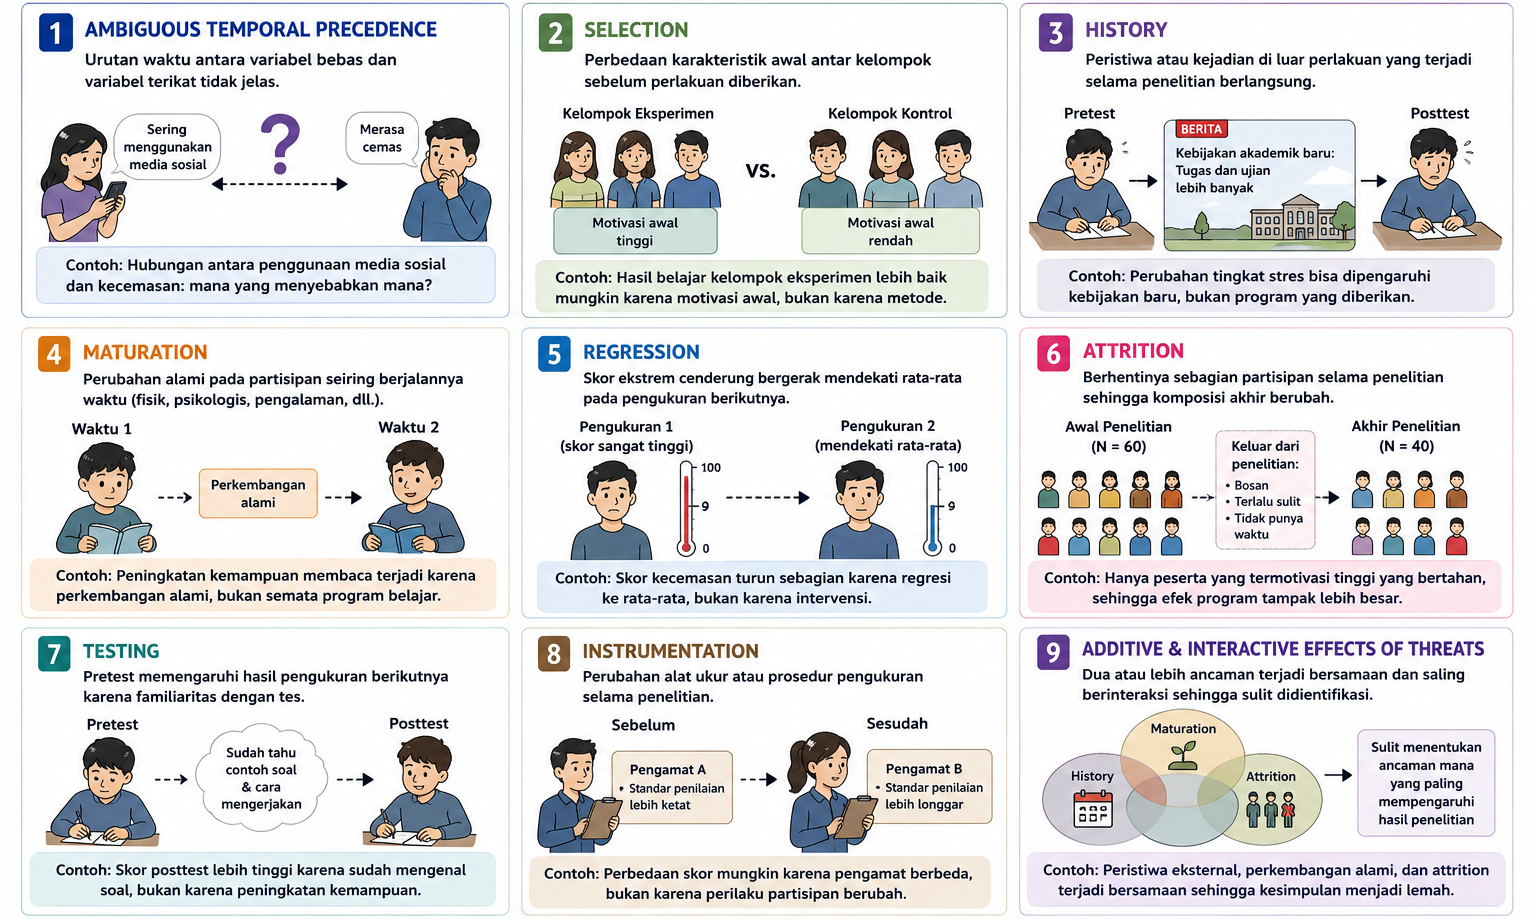
\includegraphics[keepaspectratio]{images/validitas internal.png}}
\caption{Sumber-sumber Ancaman terhadap Validitas Internal}
\end{figure}

}

\caption{\label{fig-internal}}

\end{figure}%

\subsection{Validitas Eksternal}\label{validitas-eksternal}

Jika validitas internal berkaitan dengan ketepatan hubungan sebab-akibat
yang ditemukan dalam penelitian, maka validitas eksternal berkaitan
dengan kemampuan untuk menggeneralisasikan hasil penelitian ke situasi
yang lebih luas. Dengan kata lain, validitas eksternal menjawab
pertanyaan: \emph{Apakah hasil penelitian ini juga berlaku di luar
kondisi penelitian yang dilakukan?}

Validitas eksternal menjadi penting karena tujuan penelitian tidak hanya
untuk menjelaskan fenomena pada sampel yang diteliti, tetapi juga untuk
memberikan pemahaman yang dapat diterapkan pada populasi, situasi, atau
waktu yang lebih luas. Semakin tinggi validitas eksternal suatu
penelitian, semakin besar peluang hasil penelitian tersebut dapat
digunakan dalam praktik maupun penelitian lanjutan.

Secara umum, terdapat tiga bentuk generalisasi yang menjadi perhatian
dalam validitas eksternal, yaitu:

\begin{enumerate}
\def\labelenumi{\arabic{enumi}.}
\tightlist
\item
  Generalisasi dari sampel ke populasi yang lebih luas.
\item
  Generalisasi dari situasi penelitian ke situasi dunia nyata.
\item
  Generalisasi dari satu waktu ke waktu yang berbeda.
\end{enumerate}

Beberapa faktor dapat memengaruhi validitas eksternal suatu penelitian,
yaitu validitas populasi, validitas ekologis, dan validitas temporal.

\begin{enumerate}
\def\labelenumi{\arabic{enumi}.}
\item
  \textbf{Validitas Populasi}

  Validitas populasi berkaitan dengan sejauh mana hasil penelitian dapat
  digeneralisasikan dari sampel penelitian ke populasi sasaran. Semakin
  representatif sampel terhadap populasi yang ingin diteliti, semakin
  besar peluang hasil penelitian dapat diterapkan pada populasi tersebut
  (Gravetter \& Forzano, 2018). Oleh karena itu, peneliti perlu
  mempertimbangkan karakteristik partisipan yang dipilih agar sesuai
  dengan tujuan penelitian. Beberapa hal yang memengaruhi validitas
  eksternal sebuah penelitian mencakup:

  \begin{itemize}
  \item
    Representativitas sampel

    Representativitas sampel terhadap populasi saasaran menunjukkan
    sejauh mana karakteristik sampel mencerminkan karakteristik populasi
    sasaran. Sampel yang representatif tidak selalu berarti berukuran
    besar, tetapi mampu menggambarkan karakteristik penting dari
    populasi yang diteliti (Morling, 2024). Sebagai contoh, hasil
    penelitian mengenai stres akademik yang hanya melibatkan mahasiswa
    dari satu program studi belum tentu dapat digeneralisasikan kepada
    seluruh mahasiswa di Indonesia karena karakteristik populasinya
    berbeda.
  \item
    Bias seleksi (\emph{Selection bias})

    \emph{Selection bias} terjadi ketika sampel yang digunakan tidak
    mewakili populasi sasaran. Bias ini dapat muncul karena penggunaan
    teknik \emph{convenience sampling}, rendahnya tingkat respons, atau
    karakteristik tertentu yang menyebabkan sebagian individu lebih
    mungkin menjadi partisipan (Gravetter \& Forzano, 2018). Peneliti
    dapat mengurangi bias ini dengan menggunakan teknik sampling yang
    sesuai dan menjelaskan secara terbuka keterbatasan sampel yang
    digunakan.
  \item
    Replikasi pada populasi yang berbeda

    Validitas populasi juga dapat diperkuat melalui replikasi penelitian
    pada populasi yang berbeda. Apabila hasil penelitian tetap konsisten
    ketika dilakukan pada kelompok partisipan yang memiliki
    karakteristik berbeda, maka tingkat kepercayaan terhadap kemampuan
    generalisasi hasil penelitian akan semakin tinggi (Shadish dkk.,
    2002). Oleh karena itu, replikasi menjadi salah satu cara penting
    untuk menguji apakah suatu temuan berlaku secara lebih luas.
  \end{itemize}
\item
  \textbf{Validitas Ekologis}

  Validitas ekologis menunjukkan sejauh mana kondisi penelitian
  menyerupai kondisi yang terjadi dalam kehidupan nyata. Semakin alami
  situasi penelitian, semakin besar kemungkinan hasil penelitian dapat
  diterapkan pada konteks sehari-hari (Morling, 2024).

  Sebagai contoh, penelitian mengenai perilaku belajar yang dilakukan di
  ruang kelas selama proses pembelajaran berlangsung umumnya memiliki
  validitas ekologis yang lebih tinggi dibandingkan penelitian yang
  dilakukan di laboratorium dengan kondisi yang sangat terkontrol.
  Namun, kondisi yang lebih alami sering kali membuat peneliti lebih
  sulit mengendalikan variabel-variabel pengganggu sehingga perlu
  dipertimbangkan keseimbangan antara validitas internal dan validitas
  eksternal (Creswell \& Creswell, 2023).

  Beberapa faktor yang dapat memengaruhi validitas ekologis antara lain:

  \begin{itemize}
  \item
    \emph{Multiple-treatment interference}

    \emph{Multiple-treatment interference} terjadi ketika partisipan
    menerima lebih dari satu perlakuan sehingga efek suatu perlakuan
    dipengaruhi oleh perlakuan sebelumnya. Kondisi ini menyebabkan hasil
    penelitian menjadi sulit digeneralisasikan ke situasi nyata yang
    biasanya hanya melibatkan satu jenis perlakuan (Campbell \& Stanley,
    1963).

    Sebagai contoh, peserta penelitian yang mengikuti beberapa program
    pelatihan secara berurutan mungkin menunjukkan peningkatan kemampuan
    yang berasal dari kombinasi seluruh pelatihan, bukan dari satu
    program tertentu. Untuk mengurangi ancaman ini, peneliti dapat
    memberikan jeda waktu (\emph{washout period}) atau menggunakan
    kelompok partisipan yang berbeda untuk setiap perlakuan.
  \item
    \emph{Hawthorne effect}

    \emph{Hawthorne effect} terjadi ketika partisipan mengubah
    perilakunya karena menyadari bahwa dirinya sedang diamati atau
    menjadi bagian dari suatu penelitian. Akibatnya, perilaku yang
    muncul selama penelitian belum tentu mencerminkan perilaku mereka
    dalam kondisi sehari-hari (Morling, 2024).

    Sebagai contoh, karyawan yang mengetahui bahwa produktivitasnya
    sedang diamati mungkin bekerja lebih rajin selama penelitian
    berlangsung. Peneliti dapat mengurangi efek ini dengan menciptakan
    situasi pengamatan yang senatural mungkin serta membiasakan
    partisipan terhadap kehadiran peneliti sebelum pengumpulan data
    dilakukan.
  \item
    \emph{Pretest sensitization}

    \emph{Pretest sensitization} terjadi ketika pemberian pretest
    memengaruhi respons partisipan terhadap perlakuan atau pengukuran
    berikutnya. Dalam kondisi tersebut, hasil penelitian mungkin hanya
    berlaku bagi individu yang telah mengikuti pretest sehingga
    kemampuan generalisasinya menjadi terbatas (Shadish dkk., 2002).

    Sebagai contoh, pengisian kuesioner mengenai gaya hidup sehat
    sebelum mengikuti program edukasi dapat membuat peserta lebih
    memperhatikan perilaku kesehatannya. Akibatnya, perubahan yang
    terjadi setelah intervensi mungkin dipengaruhi oleh pretest, bukan
    hanya oleh program edukasi yang diberikan. Ancaman ini dapat
    dikurangi melalui penggunaan desain \emph{Solomon Four-Group Design}
    atau dengan mempertimbangkan kembali kebutuhan penggunaan pretest.
  \end{itemize}
\item
  \textbf{Validitas Temporal}

  Validitas temporal berkaitan dengan sejauh mana hasil penelitian tetap
  berlaku apabila penelitian dilakukan pada waktu yang berbeda.
  Perubahan sosial, budaya, teknologi, maupun lingkungan dapat
  memengaruhi hubungan antarvariabel sehingga hasil penelitian yang
  valid pada suatu waktu belum tentu tetap berlaku pada waktu yang lain
  (Munger, 2019).

  Sebagai contoh, penelitian mengenai perilaku penggunaan media sosial
  yang dilakukan sepuluh tahun lalu mungkin menghasilkan temuan yang
  berbeda apabila dilakukan saat ini karena adanya perubahan platform
  digital, pola komunikasi, dan karakteristik pengguna. Oleh karena itu,
  replikasi penelitian pada periode yang berbeda menjadi salah satu cara
  untuk mengevaluasi validitas temporal suatu temuan.

  Dua bentuk variasi waktu yang sering dibahas dalam literatur adalah:

  \begin{itemize}
  \item
    \emph{Fixed-time variation}

    \emph{Fixed-time variation} mengacu pada perubahan yang terjadi
    secara teratur dan dapat diprediksi, seperti perubahan perilaku
    berdasarkan waktu dalam sehari, hari dalam seminggu, atau musim
    tertentu. Misalnya, tingkat kelelahan responden dapat berbeda antara
    pengambilan data pada pagi hari dan malam hari. Variasi tersebut
    dapat memengaruhi hasil penelitian apabila waktu pengumpulan data
    tidak diperhatikan dengan baik.
  \item
    \emph{Variable-time variation}

    \emph{Variable-time variation} merupakan perubahan yang tidak dapat
    diprediksi secara pasti, seperti perubahan kebijakan pemerintah,
    bencana alam, pandemi, atau kondisi ekonomi. Peristiwa-peristiwa
    tersebut dapat memengaruhi hasil penelitian sehingga peneliti perlu
    mempertimbangkan konteks waktu ketika menginterpretasikan maupun
    menggeneralisasikan temuan penelitian. Pandemi COVID-19 merupakan
    contoh peristiwa yang dapat mengubah perilaku masyarakat secara
    drastis sehingga hasil penelitian yang dilakukan sebelum pandemi
    belum tentu tetap berlaku setelah pandemi.
  \end{itemize}
\end{enumerate}

Secara keseluruhan, validitas eksternal menentukan sejauh mana hasil
penelitian dapat diterapkan pada populasi, situasi, dan waktu yang
berbeda dari kondisi penelitian yang dilakukan. Oleh karena itu,
peneliti perlu mempertimbangkan berbagai faktor yang dapat memengaruhi
kemampuan generalisasi hasil penelitian sejak tahap perancangan
penelitian hingga interpretasi hasil. Ringkasan mengenai berbagai faktor
yang memengaruhi validitas eksternal beserta strategi untuk
meningkatkannya disajikan pada Gambar~\ref{fig-eksternal}.

\begin{figure}

\centering{

\begin{figure}
\centering
\pandocbounded{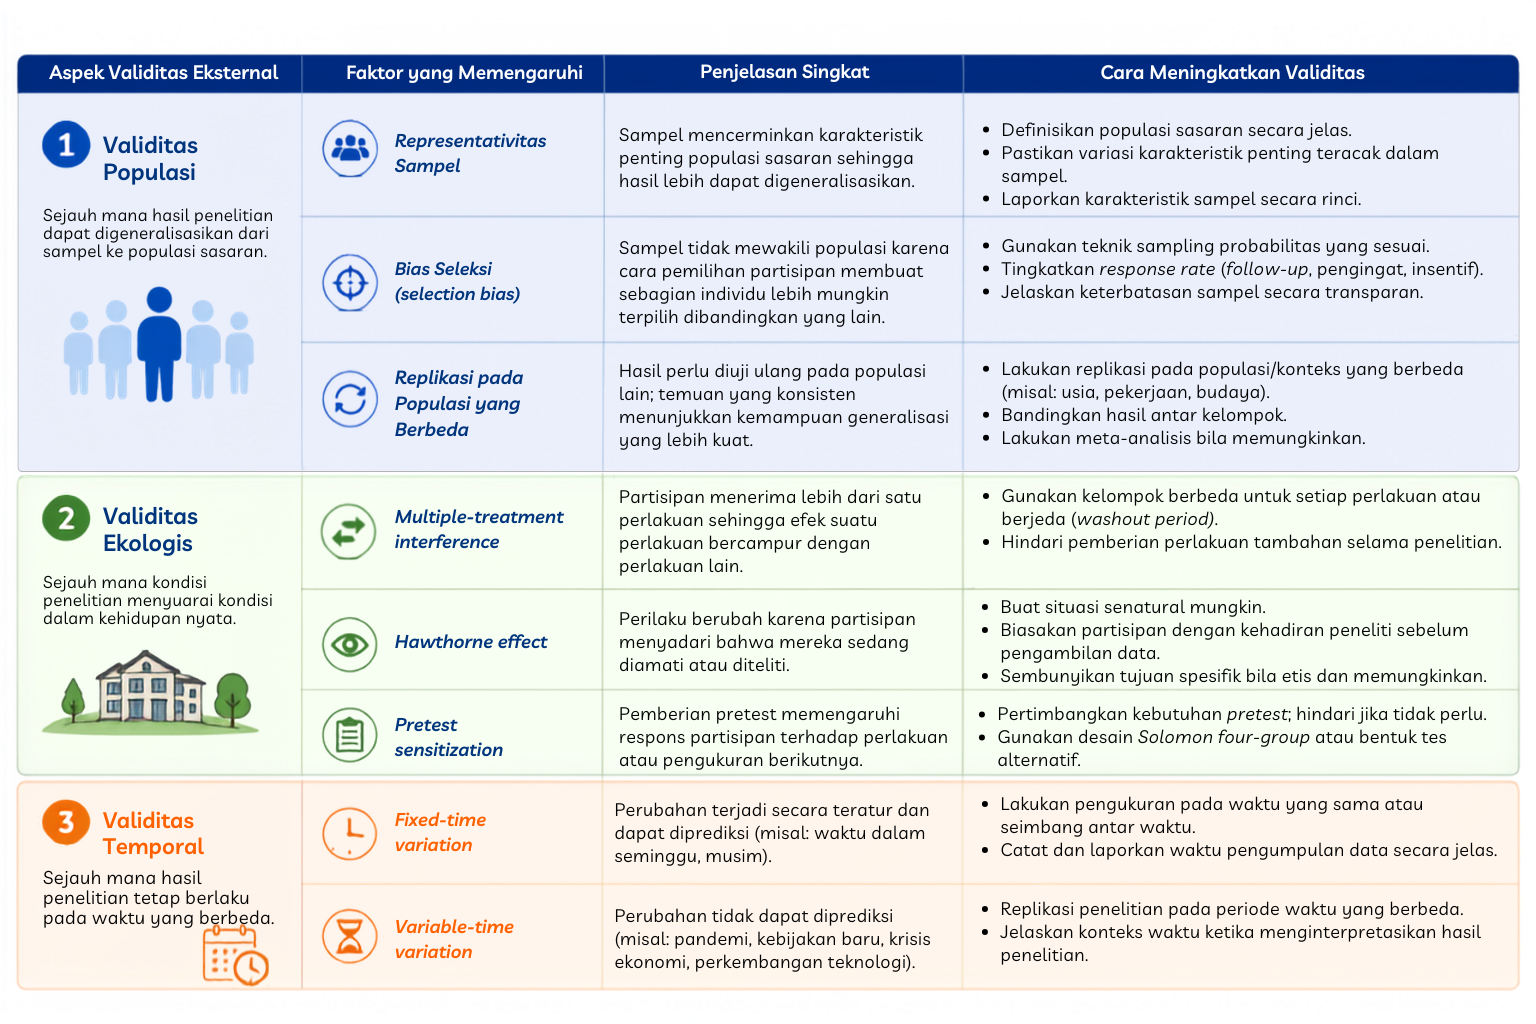
\includegraphics[keepaspectratio]{images/validitas eksternal.png}}
\caption{Ringkasan Faktor yang Memengaruhi Validitas Eksternal}
\end{figure}

}

\caption{\label{fig-eksternal}}

\end{figure}%

\begin{tcolorbox}[enhanced jigsaw, colframe=quarto-callout-tip-color-frame, toptitle=1mm, breakable, leftrule=.75mm, arc=.35mm, toprule=.15mm, colback=white, colbacktitle=quarto-callout-tip-color!10!white, bottomtitle=1mm, bottomrule=.15mm, titlerule=0mm, title=\textcolor{quarto-callout-tip-color}{\faLightbulb}\hspace{0.5em}{Rangkuman}, coltitle=black, left=2mm, opacitybacktitle=0.6, opacityback=0, rightrule=.15mm]

\begin{enumerate}
\def\labelenumi{\arabic{enumi}.}
\tightlist
\item
  Validitas menunjukkan ketepatan kesimpulan penelitian.
\item
  Validitas penelitian terdiri atas validitas internal dan validitas
  eksternal.
\item
  Validitas internal dipengaruhi oleh berbagai ancaman yang dapat
  mengganggu inferensi kausal.
\item
  Validitas eksternal berkaitan dengan kemampuan menggeneralisasikan
  hasil penelitian ke populasi, situasi, dan waktu yang berbeda.
\item
  Peneliti perlu mengendalikan berbagai ancaman terhadap validitas agar
  hasil penelitian akurat dan dapat dipercaya.
\end{enumerate}

\end{tcolorbox}

\begin{tcolorbox}[enhanced jigsaw, colframe=quarto-callout-important-color-frame, toptitle=1mm, breakable, leftrule=.75mm, arc=.35mm, toprule=.15mm, colback=white, colbacktitle=quarto-callout-important-color!10!white, bottomtitle=1mm, bottomrule=.15mm, titlerule=0mm, title=\textcolor{quarto-callout-important-color}{\faExclamation}\hspace{0.5em}{Refleksi \& Diskusi}, coltitle=black, left=2mm, opacitybacktitle=0.6, opacityback=0, rightrule=.15mm]

\begin{enumerate}
\def\labelenumi{\arabic{enumi}.}
\tightlist
\item
  Bayangkan Anda sedang meneliti efektivitas program pelatihan manajemen
  stres bagi mahasiswa. Ancaman validitas internal apa saja yang mungkin
  muncul selama penelitian berlangsung? Bagaimana cara mengatasinya?
\item
  Menurut Anda, mengapa penelitian yang dilakukan di laboratorium sering
  memiliki validitas internal yang lebih tinggi dibandingkan penelitian
  lapangan?
\item
  Sebuah penelitian menemukan bahwa penggunaan media sosial meningkatkan
  kecemasan pada remaja. Faktor-faktor apa saja yang perlu
  dipertimbangkan sebelum hasil tersebut digeneralisasikan kepada
  seluruh remaja di Indonesia?
\item
  Dalam kondisi apa peneliti sebaiknya lebih memprioritaskan validitas
  internal dibandingkan validitas eksternal? Sebaliknya, kapan validitas
  eksternal menjadi lebih penting?
\item
  Menurut Anda, apakah mungkin suatu penelitian memiliki validitas
  internal dan validitas eksternal yang sama-sama sangat tinggi?
  Jelaskan alasan Anda.
\end{enumerate}

\end{tcolorbox}

\phantomsection\label{refs--6}
\begin{CSLReferences}{1}{0}
\bibitem[\citeproctext]{ref-Campbell1963--6}
Campbell, D. T., \& Stanley, J. (1963). \emph{Experimental and
Quasi-Experimental Designs for Research}. Cengage Learning.

\bibitem[\citeproctext]{ref-Creswell2018a--6}
Creswell, J. W., \& Creswell, J. D. (2023). \emph{Research design:
Qualitative, quantitative, and mixed methods approaches} (6th ed.). SAGE
Publications.

\bibitem[\citeproctext]{ref-Gravetter2018--6}
Gravetter, F. J., \& Forzano, L. B. (2018). \emph{Research Methods for
the Behavioral Sciences} (6th ed.). Cengage Learning EMEA (UK; Europe).

\bibitem[\citeproctext]{ref-Morling2024--6}
Morling, B. (2024). \emph{Research methods in psychology : evaluating a
world of information} (4th ed.). W.W. Norton \& Company, Inc.

\bibitem[\citeproctext]{ref-Munger2019--6}
Munger, K. (2019). \emph{Knowledge Decays: Temporal Validity and Social
Science in a Changing World}.

\bibitem[\citeproctext]{ref-Shadish2002--6}
Shadish, W. R., Cook, T. D., \& Campbell, D. T. (2002).
\emph{Experimental and quasi-experimental designs for generalized causal
inference} (2nd ed.). Wadsworth/Cengage Learning.

\end{CSLReferences}

\part{PARADIGMA DALAM PENDEKATAN PENELITIAN}

\chapter{Paradigma Penelitian dalam
Psikologi}\label{paradigma-penelitian-dalam-psikologi}

\begin{tcolorbox}[enhanced jigsaw, colframe=quarto-callout-note-color-frame, toptitle=1mm, breakable, leftrule=.75mm, arc=.35mm, toprule=.15mm, colback=white, colbacktitle=quarto-callout-note-color!10!white, bottomtitle=1mm, bottomrule=.15mm, titlerule=0mm, title=\textcolor{quarto-callout-note-color}{\faInfo}\hspace{0.5em}{Tujuan Pembelajaran}, coltitle=black, left=2mm, opacitybacktitle=0.6, opacityback=0, rightrule=.15mm]

Setelah mempelajari bab ini, mahasiswa diharapkan mampu:

\begin{enumerate}
\def\labelenumi{\arabic{enumi}.}
\tightlist
\item
  Menjelaskan pengertian dan peran paradigma dalam penelitian psikologi.
\item
  Membedakan paradigma penelitian dengan metode penelitian.
\item
  Menjelaskan tiga pilar filosofis paradigma penelitian, yaitu ontologi,
  epistemologi, dan metodologi.
\item
  Mengidentifikasi karakteristik utama paradigma positivisme,
  post-positivisme, interpretivisme, dan transformatif.
\item
  Membandingkan keempat paradigma penelitian berdasarkan asumsi
  filosofis, tujuan penelitian, dan implikasi metodologisnya.
\end{enumerate}

\end{tcolorbox}

\section{Konsep Dasar Paradigma
Penelitian}\label{konsep-dasar-paradigma-penelitian}

Setiap penelitian didasarkan pada cara pandang tertentu mengenai hakikat
realitas, cara memperoleh pengetahuan, dan bagaimana penelitian
seharusnya dilakukan. Cara pandang tersebut dikenal sebagai
\textbf{paradigma penelitian}. Pemahaman terhadap paradigma penting
karena memengaruhi seluruh proses penelitian, mulai dari perumusan
masalah hingga interpretasi hasil. Bab ini membahas konsep paradigma
penelitian, tiga pilar filosofis yang mendasarinya, serta empat
paradigma utama yang digunakan dalam penelitian psikologi.

\subsection{Mengapa Paradigma Penting?}\label{mengapa-paradigma-penting}

Bayangkan empat orang peneliti ingin meneliti fenomena yang sama, yaitu
\emph{burnout} pada tenaga kesehatan.

\begin{quote}
Peneliti pertama bertanya, ``Seberapa tinggi tingkat \emph{burnout} pada
perawat?''\\
Peneliti kedua bertanya, ``Faktor apa yang paling memprediksi
\emph{burnout}?''\\
Peneliti ketiga bertanya, ``Bagaimana perawat memaknai pengalaman
\emph{burnout} yang mereka alami?''\\
Peneliti keempat bertanya, ``Bagaimana sistem pelayanan kesehatan
berkontribusi terhadap munculnya burnout, dan bagaimana kondisi tersebut
dapat diubah?''
\end{quote}

Keempat pertanyaan tersebut sama-sama berkaitan dengan \emph{burnout},
tetapi berangkat dari cara pandang yang berbeda mengenai hakikat
realitas, tujuan penelitian, dan cara memperoleh pengetahuan. Cara
pandang yang berbeda inilah yang dalam metodologi penelitian disebut
paradigma penelitian.

\subsection{Definisi Paradigma
Penelitian}\label{definisi-paradigma-penelitian}

Istilah paradigma (dari bahasa Yunani: \emph{paradeigma}, berarti
``pola'' atau ``contoh'') dipopulerkan dalam filsafat ilmu oleh Thomas
S. Kuhn melalui karyanya yang monumental, \emph{The Structure of
Scientific Revolutions}. Kuhn menggunakan istilah ini untuk
menggambarkan kerangka konseptual bersama yang dianut komunitas ilmuwan
dalam periode tertentu --- sebuah ``cara melihat dunia'' yang diterima
secara kolektif.

Dalam konteks penelitian ilmu sosial dan psikologi, definisi yang paling
operasional dikemukakan oleh Guba \& Lincoln (1994):

\begin{quote}
``\emph{A paradigm may be viewed as a set of basic beliefs (or
metaphysics) that deals with ultimates or first principles. It
represents a worldview that defines, for its holder, the nature of the
`world', the individual's place in it, and the range of possible
relationships to that world and its parts.}'' {[}hal. 107{]}
\end{quote}

Dengan kata lain, paradigma penelitian adalah sistem kepercayaan
mendasar yang tidak dapat dibuktikan atau dipatahkan secara empiris
semata, karena merupakan fondasi yang mendahului proses empiris itu
sendiri. Paradigma penelitian menjawab pertanyaan paling fundamental
sebelum seorang peneliti bahkan mulai mengumpulkan data.

Dengan demikian, paradigma tidak sekadar menentukan metode penelitian
yang digunakan, tetapi juga memengaruhi cara peneliti merumuskan
masalah, memilih desain penelitian, mengumpulkan data, menganalisis
temuan, hingga menarik kesimpulan.

\subsection{Paradigma dan Proses
Penelitian}\label{paradigma-dan-proses-penelitian}

Paradigma penelitian merupakan landasan filosofis yang mendasari seluruh
proses penelitian. Paradigma memengaruhi cara peneliti memandang suatu
fenomena, merumuskan masalah penelitian, menentukan pendekatan dan
desain penelitian, memilih metode pengumpulan serta analisis data,
hingga menginterpretasikan hasil penelitian. Oleh karena itu, setiap
keputusan metodologis dalam penelitian sebaiknya konsisten dengan
paradigma yang digunakan.

Hubungan antara paradigma dan keseluruhan proses penelitian ditunjukkan
pada Gambar~\ref{fig-proses}.

\begin{figure}

\centering{

\begin{figure}
\centering
\pandocbounded{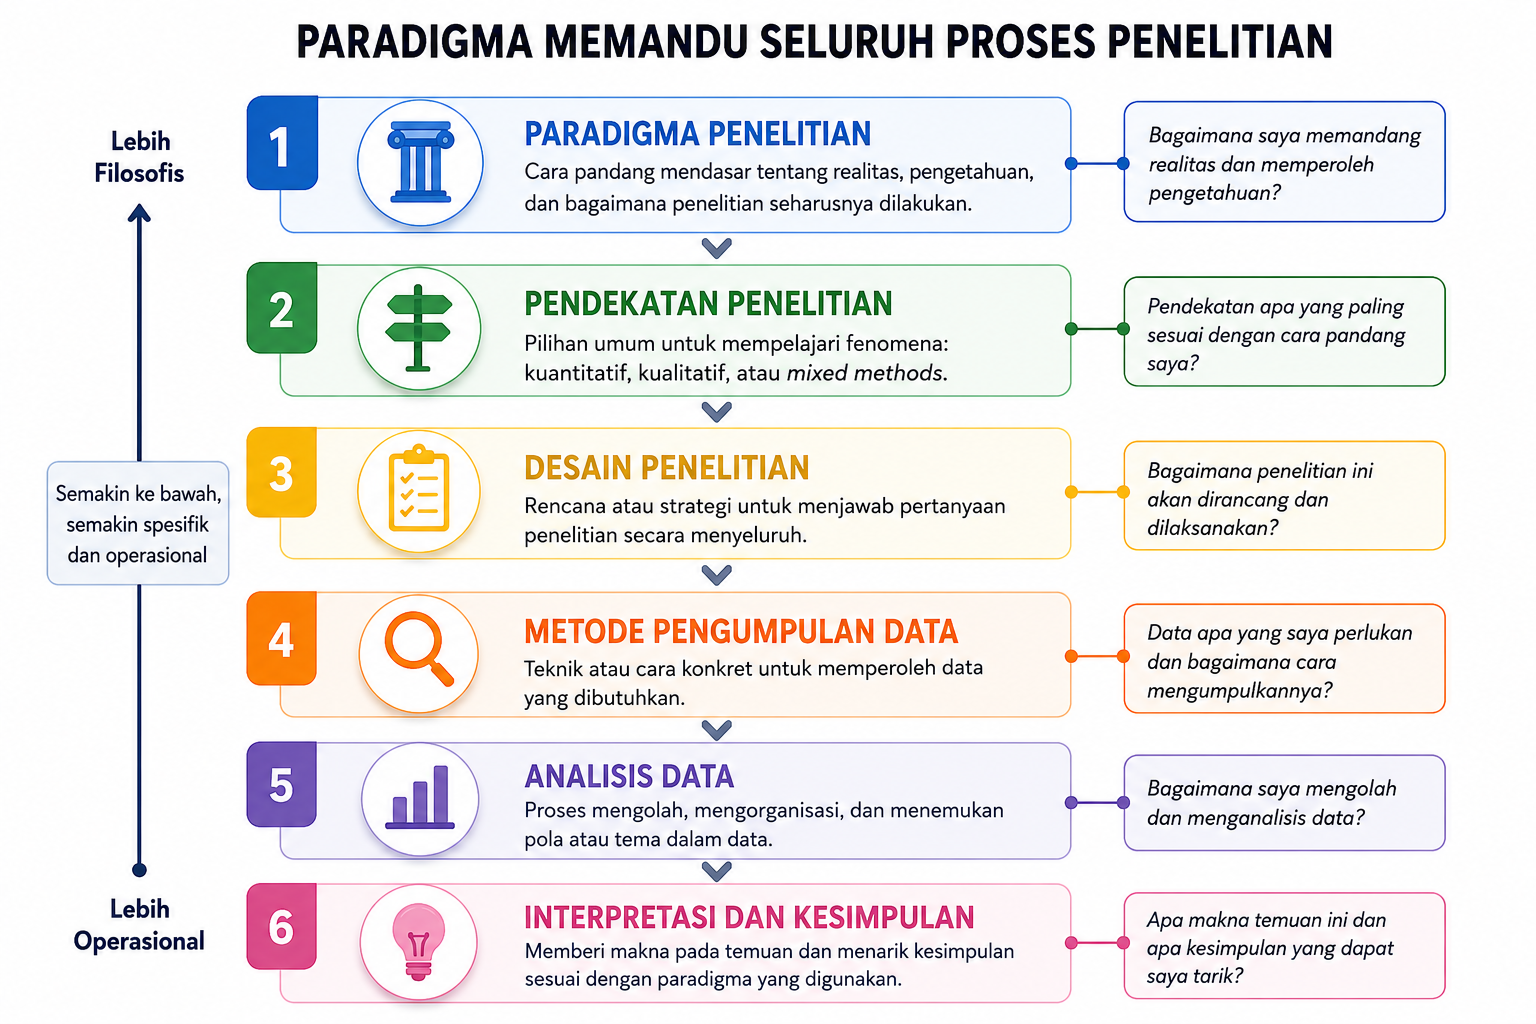
\includegraphics[keepaspectratio]{images/paradigma - bab 9.png}}
\caption{Paradigma sebagai Landasan Proses Penelitian}
\end{figure}

}

\caption{\label{fig-proses}}

\end{figure}%

Meskipun terdapat berbagai paradigma penelitian, semuanya berangkat dari
asumsi filosofis yang berbeda mengenai hakikat realitas, cara memperoleh
pengetahuan, dan cara melakukan penelitian. Perbedaan tersebut akan
dibahas pada bagian-bagian berikutnya di bab ini.

\subsection{Paradigma vs.~Metode}\label{paradigma-vs.-metode}

Paradigma penelitian sering kali disamakan dengan metode penelitian,
padahal keduanya merupakan konsep yang berbeda. Paradigma merupakan
landasan filosofis yang memengaruhi cara peneliti memandang realitas,
memperoleh pengetahuan, dan merancang penelitian secara keseluruhan,
sedangkan metode adalah teknik atau prosedur yang digunakan untuk
mengumpulkan dan menganalisis data.

Dengan demikian, paradigma menjadi dasar dalam pemilihan metode yang
sesuai dengan tujuan dan asumsi penelitian. Perbedaan antara paradigma
dan metode penelitian dirangkum pada Tabel~\ref{tbl-paradigma}.

\begin{longtable}[]{@{}
  >{\raggedright\arraybackslash}p{(\linewidth - 4\tabcolsep) * \real{0.3333}}
  >{\raggedright\arraybackslash}p{(\linewidth - 4\tabcolsep) * \real{0.3333}}
  >{\raggedright\arraybackslash}p{(\linewidth - 4\tabcolsep) * \real{0.3333}}@{}}
\caption{Perbedaan Paradigma dan
Metode}\label{tbl-paradigma}\tabularnewline
\toprule\noalign{}
\endfirsthead
\endhead
\bottomrule\noalign{}
\endlastfoot
\textbf{Dimensi} & \textbf{Paradigma} & \textbf{Metode} \\
Sifat & Filosofis/keyakinan mendasar & Teknis/prosedural \\
Pertanyaan yang dijawab & ``Apa hakikat realitas yang saya teliti dan
bagaimana saya dapat mengetahuinya?'' & ``Bagaimana cara terbaik
mengumpulkan dan menganalisis data?'' \\
Level abstraksi & Abstrak, tidak tampak langsung dalam laporan
penelitian & Konkret, tampak dalam bagian metode laporan penelitian \\
Dapat diganti sewaktu-waktu? & Tidak, perubahan paradigma bersifat
mendasar dan memerlukan reorientasi intelektual & Ya, metode dapat
disesuaikan dengan kebutuhan tanpa mengubah paradigma \\
\end{longtable}

Setiap paradigma dibangun di atas asumsi filosofis tertentu. Untuk
memahaminya, kita perlu mengenal tiga pilar filosofis paradigma
penelitian.

\section{Tiga Pilar Filosofis Paradigma
Penelitian}\label{tiga-pilar-filosofis-paradigma-penelitian}

Sebagaimana telah dijelaskan pada bagian sebelumnya, paradigma menjadi
landasan bagi seluruh proses penelitian. Perbedaan antarparadigma pada
dasarnya berasal dari perbedaan asumsi filosofis yang dianut peneliti.
Asumsi tersebut umumnya dapat dipahami melalui tiga pilar utama, yaitu
\textbf{ontologi}, \textbf{epistemologi}, dan \textbf{metodologi}
(Creswell \& Creswell, 2023; Guba \& Lincoln, 1994).

\subsection{Ontologi}\label{ontologi}

Ontologi membahas hakikat realitas yang menjadi objek penelitian. Dengan
kata lain, ontologi menjawab pertanyaan:

\begin{quote}
\emph{``Apa hakikat realitas yang sedang saya teliti?''}
\end{quote}

Dalam penelitian psikologi, pertanyaan ontologis berkaitan dengan
bagaimana peneliti memandang suatu fenomena psikologis, seperti
kecerdasan, motivasi, atau kesehatan mental. Perbedaan pandangan
mengenai hakikat realitas inilah yang menjadi salah satu pembeda utama
antarparadigma penelitian.

\subsection{Epistemologi}\label{epistemologi}

Epistemologi membahas bagaimana pengetahuan mengenai suatu realitas
dapat diperoleh. Pertanyaan utama yang dijawab adalah:

\begin{quote}
\emph{``Bagaimana saya dapat mengetahui realitas yang sedang saya
teliti?''}
\end{quote}

Dalam penelitian, epistemologi berkaitan dengan hubungan antara peneliti
dan objek penelitian, serta cara memperoleh data atau informasi yang
dapat dipercaya. Perbedaan pandangan epistemologis akan memengaruhi
bagaimana penelitian dilakukan dan bagaimana hasilnya diinterpretasikan.

\subsection{Metodologi}\label{metodologi}

Metodologi menjelaskan strategi atau pendekatan umum yang digunakan
untuk memperoleh pengetahuan mengenai suatu fenomena. Dengan demikian,
metodologi menjawab pertanyaan:

\begin{quote}
\emph{``Bagaimana penelitian harus dilakukan agar pengetahuan tersebut
dapat diperoleh?''}
\end{quote}

Perlu dibedakan bahwa metodologi bukanlah metode penelitian. Metodologi
merupakan kerangka atau logika penelitian yang didasarkan pada asumsi
filosofis tertentu, sedangkan metode adalah teknik yang digunakan untuk
mengumpulkan dan menganalisis data.

\begin{figure}

\centering{

\begin{figure}
\centering
\pandocbounded{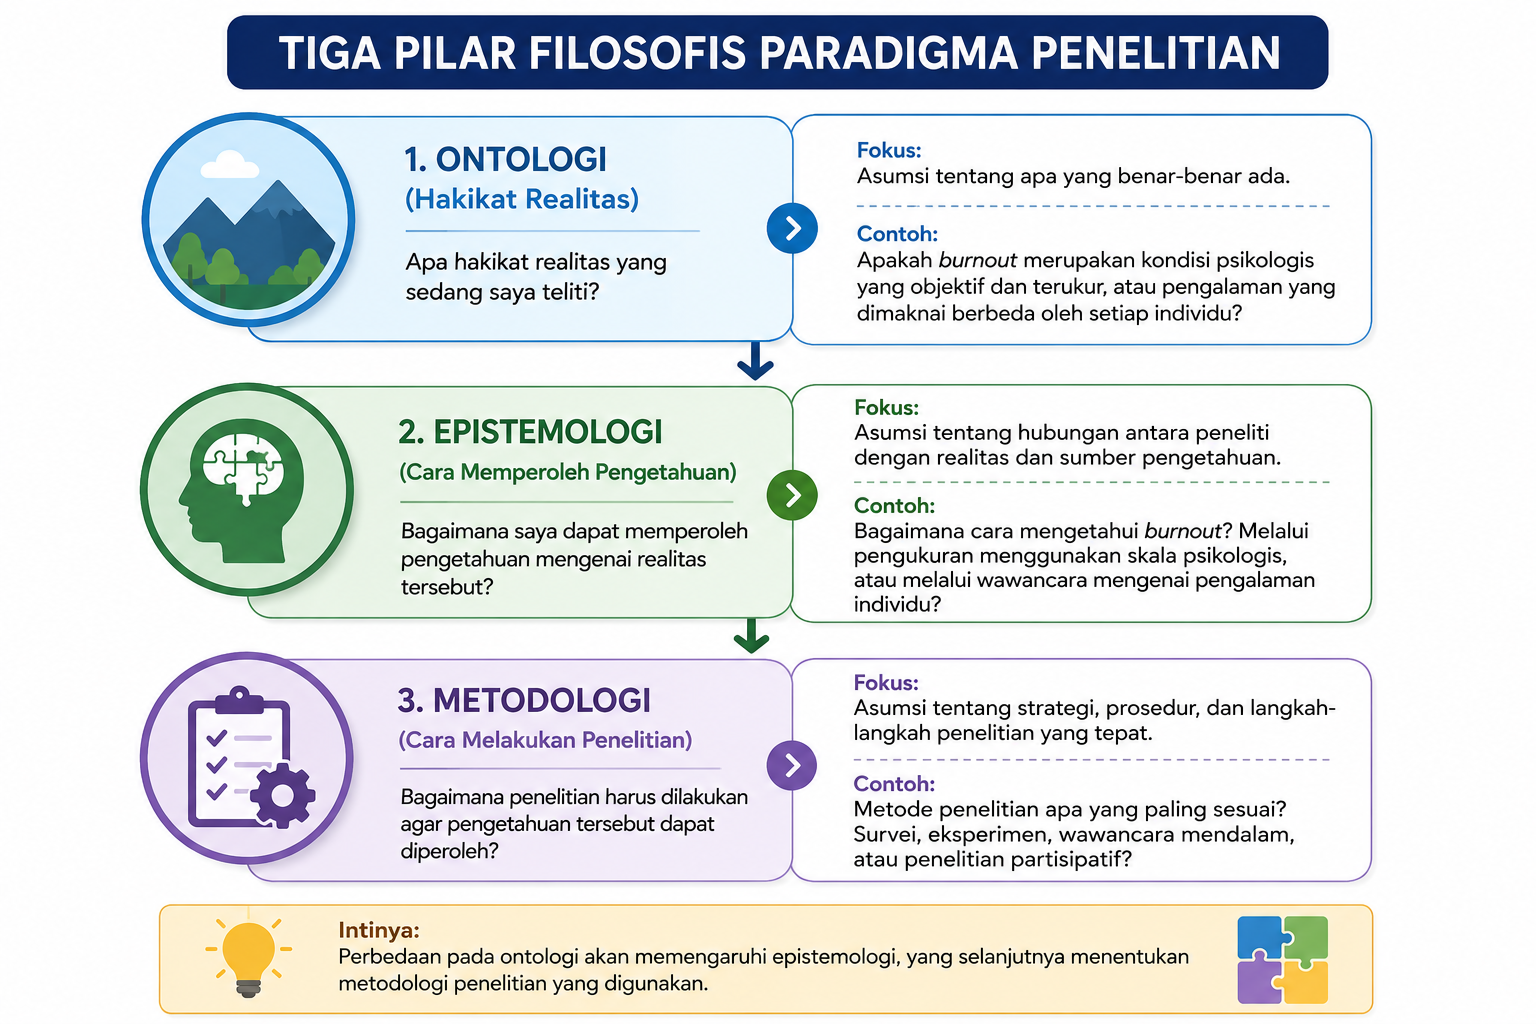
\includegraphics[keepaspectratio]{images/pilar filososif - bab 9.png}}
\caption{Hubungan Ontologi, Epistemologi, dan Metodologi}
\end{figure}

}

\caption{\label{fig-pilar}}

\end{figure}%

Gambar~\ref{fig-pilar} menunjukkan bahwa ontologi, epistemologi, dan
metodologi merupakan tiga pilar filosofis yang saling berkaitan.
Perbedaan pandangan terhadap ketiga aspek inilah yang kemudian
melahirkan berbagai paradigma penelitian. Pada bagian berikutnya akan
dibahas empat paradigma utama yang banyak digunakan dalam penelitian
psikologi.

\section{Empat Paradigma Utama dalam Penelitian
Psikologi}\label{empat-paradigma-utama-dalam-penelitian-psikologi}

Perbedaan pandangan mengenai ontologi, epistemologi, dan metodologi
melahirkan berbagai paradigma penelitian. Setiap paradigma menawarkan
cara pandang yang berbeda dalam memahami fenomena psikologis serta
memiliki implikasi terhadap pemilihan pendekatan, desain, dan metode
penelitian. Bagian ini membahas empat paradigma utama yang banyak
digunakan dalam penelitian psikologi, yaitu \textbf{positivisme,
post-positivisme, interpretivisme,} dan \textbf{transformatif}.

\subsection{Paradigma Positivisme}\label{paradigma-positivisme}

\subsubsection{Akar Historis dan Tokoh
Kunci}\label{akar-historis-dan-tokoh-kunci}

Paradigma positivisme berkembang pada abad ke-19 seiring munculnya
keyakinan bahwa fenomena alam maupun sosial dapat dipelajari melalui
observasi empiris, pengukuran, dan penalaran logis. Tokoh yang paling
sering dikaitkan dengan paradigma ini adalah Auguste Comte, yang
berpendapat bahwa pengetahuan ilmiah harus didasarkan pada fakta-fakta
yang dapat diamati, bukan pada spekulasi metafisis (Crotty, 1998).

Dalam psikologi, pengaruh positivisme tampak sejak berdirinya
laboratorium psikologi eksperimental oleh Wilhelm Wundt di Leipzig pada
tahun 1879, yang menandai berkembangnya psikologi sebagai disiplin
ilmiah yang menggunakan metode eksperimental. Tradisi ini kemudian
diperkuat oleh perkembangan psikometri dan behaviorisme yang menekankan
pengukuran objektif, pengendalian variabel, dan pengujian hipotesis
secara empiris (Goodwin, 2022).

\subsubsection{Kekuatan dan
Keterbatasan}\label{kekuatan-dan-keterbatasan}

\textbf{Kekuatan:}

\begin{itemize}
\tightlist
\item
  Menghasilkan pengetahuan yang dapat direplikasi dan digeneralisasi.
\item
  Memungkinkan komparasi lintas populasi dan waktu.
\item
  Menjadi basis legitimasi ilmiah psikologi di antara ilmu-ilmu alam.
\item
  Produktif untuk penelitian dasar (basic research) tentang proses
  kognitif, perseptual, dan neurologis.
\end{itemize}

\textbf{Keterbatasan:}

\begin{itemize}
\tightlist
\item
  Menempatkan realitas manusia seolah setara dengan realitas fisik,
  padahal manusia adalah makhluk yang bermakna
  (\emph{meaning}-\emph{making}).
\item
  Cenderung mereduksi kompleksitas pengalaman manusia menjadi
  angka-angka yang kehilangan konteks.
\item
  Menafikan peran konteks budaya, sejarah, dan kuasa dalam membentuk
  fenomena psikologis.
\item
  Rentan terhadap bias positivistik tersembunyi dalam alat ukur.
\end{itemize}

\subsection{Paradigma
Post-Positivisme}\label{paradigma-post-positivisme}

\subsubsection{Akar Historis dan Tokoh
Kunci}\label{akar-historis-dan-tokoh-kunci-1}

Post-positivisme berkembang pada pertengahan abad ke-20 sebagai
penyempurnaan terhadap positivisme klasik. Paradigma ini tetap meyakini
adanya realitas objektif, tetapi mengakui bahwa pengetahuan manusia
mengenai realitas tersebut selalu bersifat sementara, tidak sempurna,
dan terbuka untuk direvisi berdasarkan bukti baru (Phillips \& Burbules,
2000).

Perkembangan paradigma ini dipengaruhi oleh pemikiran Karl Popper
mengenai falsifikasi, Thomas Kuhn mengenai perubahan paradigma ilmiah,
serta berbagai perkembangan dalam filsafat ilmu modern yang menunjukkan
bahwa observasi dan pengukuran tidak pernah sepenuhnya bebas dari
keterbatasan (Kuhn, 1996; Popper, 2005). Dalam penelitian psikologi
kontemporer, post-positivisme menjadi paradigma yang paling dominan
karena memungkinkan penggunaan metode ilmiah secara ketat sekaligus
mengakui adanya ketidakpastian, kesalahan pengukuran, dan kemungkinan
bias peneliti (Guba \& Lincoln, 1994). Hingga saat ini, prinsip-prinsip
post-positivisme masih menjadi landasan utama dalam sebagian besar
penelitian kuantitatif di bidang psikologi (Creswell \& Creswell, 2023).

\subsubsection{Kekuatan dan
Keterbatasan}\label{kekuatan-dan-keterbatasan-1}

\textbf{Kekuatan:}

\begin{itemize}
\tightlist
\item
  Tetap mempertahankan ketelitian metode ilmiah sambil mengakui adanya
  keterbatasan pengukuran dan bias peneliti.
\item
  Mendorong pengujian teori secara kritis melalui falsifikasi,
  replikasi, dan triangulasi.
\item
  Menjadi landasan utama bagi sebagian besar penelitian kuantitatif
  modern dalam psikologi.
\end{itemize}

\textbf{Keterbatasan:}

\begin{itemize}
\tightlist
\item
  Tetap berfokus pada pengujian teori sehingga kurang mampu menangkap
  makna subjektif dan konteks sosial secara mendalam.
\item
  Objektivitas yang diupayakan tetap tidak dapat sepenuhnya
  menghilangkan pengaruh asumsi dan interpretasi peneliti.
\item
  Kurang sesuai untuk penelitian yang bertujuan memahami pengalaman
  individual atau mendorong perubahan sosial.
\end{itemize}

\subsection{Paradigma
Interpretivisme/Konstruktivisme}\label{paradigma-interpretivismekonstruktivisme}

\subsubsection{Akar Historis dan Tokoh
Kunci}\label{akar-historis-dan-tokoh-kunci-2}

Interpretivisme berkembang sebagai respons terhadap keterbatasan
pendekatan positivistik dalam memahami pengalaman manusia. Paradigma ini
berangkat dari pandangan bahwa manusia bukan sekadar obyek yang dapat
diukur, tetapi individu yang secara aktif membangun dan memberi makna
terhadap pengalaman hidupnya. Oleh karena itu, penelitian berupaya
memahami perspektif partisipan dalam konteks kehidupannya (Creswell \&
Clark, 2018; Crotty, 1998).

Akar filosofis paradigma ini berasal dari tradisi hermeneutika,
fenomenologi, dan sosiologi interpretatif yang dikembangkan oleh
tokoh-tokoh seperti Wilhelm Dilthey, Max Weber, Edmund Husserl, dan
Martin Heidegger (Laverty, 2003). Dalam psikologi, paradigma ini menjadi
landasan berkembangnya berbagai pendekatan penelitian kualitatif yang
berfokus pada pengalaman subjektif, makna, dan konteks sosial (Willig \&
Rogers, 2021).

Paradigma ini menjadi landasan berkembangnya berbagai pendekatan
penelitian kualitatif, seperti fenomenologi, \emph{grounded theory},
etnografi, studi naratif, dan analisis tematik, yang akan dibahas lebih
mendalam pada Bab~\ref{sec-desainkuali}.

\subsubsection{Kekuatan dan
Keterbatasan}\label{kekuatan-dan-keterbatasan-2}

\textbf{Kekuatan:}

\begin{itemize}
\tightlist
\item
  Menangkap kedalaman, kompleksitas, dan kontekstualism pengalaman
  manusia yang tidak dapat diangkakan.
\item
  Menghasilkan teori yang kaya dan ``hidup'' karena berakar pada
  realitas partisipan.
\item
  Sangat berguna untuk memahami fenomena baru atau yang kurang dipahami.
\item
  Memungkinkan suara kelompok yang terpinggirkan terdengar.
\end{itemize}

\textbf{Keterbatasan:}

\begin{itemize}
\tightlist
\item
  Hasil sulit digeneralisasi secara statistis ke populasi yang lebih
  luas.
\item
  Memerlukan waktu dan keahlian yang lebih intensif.
\item
  Rentan terhadap bias peneliti jika refleksivitas tidak dijaga.
\item
  Sering menghadapi pertanyaan legitimasi ilmiah dari komunitas
  positivis.
\end{itemize}

\subsection{Paradigma Transformatif
(Kritis)}\label{paradigma-transformatif-kritis}

\subsubsection{Akar Historis dan Tokoh
Kunci}\label{akar-historis-dan-tokoh-kunci-3}

Paradigma transformatif berkembang dari tradisi Teori Kritis
(\emph{Critical Theory}) yang muncul pada awal abad ke-20 melalui
pemikiran para ilmuwan \emph{Frankfurt School}, terutama Max Horkheimer,
Theodor Adorno, dan kemudian Jürgen Habermas. Berbeda dengan positivisme
yang berupaya menjelaskan dan memprediksi fenomena secara objektif,
Teori Kritis memandang bahwa ilmu pengetahuan tidak pernah sepenuhnya
bebas nilai. Pengetahuan selalu dipengaruhi oleh konteks sosial,
politik, ekonomi, dan budaya, serta dapat digunakan baik untuk
mempertahankan maupun menantang struktur kekuasaan yang ada (Habermas,
1971; Horkheimer, 1972).

Paradigma ini kemudian berkembang melalui berbagai perspektif seperti
pedagogi kritis, teori feminis, teori ras kritis, studi disabilitas, dan
psikologi \emph{indigenous}. Kesamaan dari berbagai pendekatan tersebut
adalah keyakinan bahwa penelitian tidak cukup hanya menghasilkan
pengetahuan, tetapi juga perlu berkontribusi pada pemberdayaan individu
maupun komunitas serta mendorong perubahan sosial yang lebih adil
(Mertens, 2024).

Dalam psikologi, paradigma transformatif menjadi landasan berkembangnya
berbagai bidang seperti psikologi komunitas, psikologi feminis,
psikologi \emph{indigenous}, serta berbagai bentuk penelitian
partisipatif, misalnya \emph{Participatory Action Research} (PAR) dan
\emph{Community-Based Participatory Research} (CBPR). Dalam paradigma
ini, partisipan dipandang sebagai mitra penelitian yang aktif, sehingga
proses penelitian diharapkan tidak hanya menghasilkan pemahaman ilmiah,
tetapi juga memberikan manfaat nyata bagi individu maupun masyarakat
yang terlibat.

\subsubsection{Kekuatan dan
Keterbatasan}\label{kekuatan-dan-keterbatasan-3}

\textbf{Kekuatan:}

\begin{itemize}
\tightlist
\item
  Mengungkap pengaruh faktor sosial, budaya, dan relasi kekuasaan
  terhadap fenomena psikologis.
\item
  Berorientasi pada pemberdayaan individu dan komunitas serta mendorong
  perubahan sosial yang lebih adil.
\item
  Relevan untuk penelitian pada kelompok rentan atau komunitas yang
  kurang terwakili.
\end{itemize}

\textbf{Keterbatasan:}

\begin{itemize}
\tightlist
\item
  Keterlibatan peneliti yang tinggi dapat meningkatkan potensi bias dan
  mengurangi objektivitas.
\item
  Proses penelitian umumnya memerlukan waktu, kolaborasi, dan sumber
  daya yang lebih besar.
\item
  Temuan sering kali bersifat kontekstual sehingga transferabilitasnya
  ke konteks lain perlu dipertimbangkan secara hati-hati.
\end{itemize}

Keempat paradigma yang telah dipaparkan di atas memiliki karakteristik,
asumsi filosofis, dan implikasi metodologis yang berbeda. Ringkasan
perbandingan keempat paradigma disajikan pada
Tabel~\ref{tbl-komparasiparadigma}.

\begin{longtable}[]{@{}
  >{\raggedright\arraybackslash}p{(\linewidth - 8\tabcolsep) * \real{0.2000}}
  >{\raggedright\arraybackslash}p{(\linewidth - 8\tabcolsep) * \real{0.2000}}
  >{\raggedright\arraybackslash}p{(\linewidth - 8\tabcolsep) * \real{0.2000}}
  >{\raggedright\arraybackslash}p{(\linewidth - 8\tabcolsep) * \real{0.2000}}
  >{\raggedright\arraybackslash}p{(\linewidth - 8\tabcolsep) * \real{0.2000}}@{}}
\caption{Perbandingan Empat Paradigma
Penelitian}\label{tbl-komparasiparadigma}\tabularnewline
\toprule\noalign{}
\endfirsthead
\endhead
\bottomrule\noalign{}
\endlastfoot
\textbf{Dimensi} & \textbf{Positivisme} & \textbf{Post-Positivisme} &
\textbf{Interpretivisme} & \textbf{Transformatif} \\
Ontologi & Realisme naif & Realisme kritis & Relativisme & Realisme
historis \\
Epistemologi & Dualisme objektif & Obyektivitas dimodifikasi &
Subyektivitas transaksional & Intersubyektivitas kritis \\
Metodologi & Deduktif, eksperimental, pengujian hipotesis, pengukuran
objektif. & Deduktif-falsifikatif, pengujian teori secara kritis,
triangulasi, replikasi, dan pengendalian bias. & Induktif, eksploratif,
interpretatif, berfokus pada pengalaman dan makna. & Partisipatif,
kolaboratif, reflektif, berorientasi pada aksi dan perubahan sosial. \\
Tujuan penelitian & Hukum universal, prediksi & Teori probabilistik,
kontrol variabel & Pemahaman mendalam, teori lokal & Perubahan sosial,
pemberdayaan \\
Kekuatan & objektif, terukur, dan hasilnya mudah digeneralisasi. & Lebih
realistis karena mengakui keterbatasan pengukuran dan potensi bias. &
Memberikan pemahaman yang mendalam terhadap pengalaman dan makna. &
Mendorong pemberdayaan serta perubahan sosial yang berkeadilan. \\
Keterbatasan & Kurang mampu menangkap makna subjektif dan konteks
sosial. & Objektivitas tetap tidak dapat dicapai secara sempurna. &
Temuan sulit digeneralisasi dan sangat bergantung pada konteks. & Rentan
terhadap bias nilai serta memerlukan kolaborasi dan sumber daya yang
lebih besar. \\
\end{longtable}

\begin{tcolorbox}[enhanced jigsaw, colframe=quarto-callout-tip-color-frame, toptitle=1mm, breakable, leftrule=.75mm, arc=.35mm, toprule=.15mm, colback=white, colbacktitle=quarto-callout-tip-color!10!white, bottomtitle=1mm, bottomrule=.15mm, titlerule=0mm, title=\textcolor{quarto-callout-tip-color}{\faLightbulb}\hspace{0.5em}{Tips Memilih Paradigma}, coltitle=black, left=2mm, opacitybacktitle=0.6, opacityback=0, rightrule=.15mm]

Paradigma penelitian tidak dipilih berdasarkan mana yang paling baik,
melainkan berdasarkan kesesuaiannya dengan tujuan penelitian, pertanyaan
penelitian, dan karakteristik fenomena yang diteliti. Oleh karena itu,
peneliti perlu memastikan bahwa paradigma, pendekatan, desain, dan
metode penelitian yang dipilih membentuk suatu rangkaian yang konsisten.

\end{tcolorbox}

\section{\texorpdfstring{Pragmatisme dan Perkembangan \emph{Mixed
methods}}{Pragmatisme dan Perkembangan Mixed methods}}\label{pragmatisme-dan-perkembangan-mixed-methods}

\subsection{\texorpdfstring{Lahirnya Pendekatan \emph{Mixed
methods}}{Lahirnya Pendekatan Mixed methods}}\label{lahirnya-pendekatan-mixed-methods}

Selama beberapa dekade, penelitian sosial diwarnai oleh perdebatan yang
dikenal sebagai \emph{paradigm wars}, yaitu perdebatan mengenai
paradigma mana yang paling tepat digunakan dalam penelitian ilmiah.
Pendukung pendekatan kuantitatif yang berakar pada positivisme atau
post-positivisme berpendapat bahwa realitas dapat dipelajari secara
objektif melalui pengukuran dan analisis statistik.

Sebaliknya, pendukung pendekatan kualitatif yang berakar pada
interpretivisme menekankan bahwa pemahaman terhadap pengalaman manusia
memerlukan eksplorasi makna dan konteks sosial. Perdebatan tersebut
berlangsung cukup lama hingga muncul pandangan bahwa kedua pendekatan
sebenarnya tidak selalu harus dipertentangkan, melainkan dapat saling
melengkapi untuk menjawab pertanyaan penelitian yang kompleks (Creswell
\& Creswell, 2023).

\subsection{Pragmatisme sebagai Fondasi
Filosofis}\label{pragmatisme-sebagai-fondasi-filosofis}

Salah satu landasan filosofis yang paling banyak digunakan dalam
penelitian \emph{mixed methods} adalah pragmatisme. Berbeda dengan
paradigma lain yang berangkat dari asumsi filosofis mengenai hakikat
realitas, pragmatisme lebih menekankan penyelesaian masalah penelitian
secara praktis. Fokus utamanya bukan pada perdebatan apakah realitas
bersifat objektif atau dikonstruksi secara sosial, melainkan pada
penggunaan pendekatan yang paling tepat untuk menjawab pertanyaan
penelitian (Creswell \& Creswell, 2023).

\subsection{\texorpdfstring{Hubungan Pragmatisme dengan \emph{Mixed
methods}}{Hubungan Pragmatisme dengan Mixed methods}}\label{hubungan-pragmatisme-dengan-mixed-methods}

Karena pragmatisme berorientasi pada pemecahan masalah, paradigma ini
memberikan ruang bagi penggunaan berbagai metode penelitian secara
terpadu. Dalam praktiknya, seorang peneliti dapat mengombinasikan
pengumpulan data kuantitatif dan kualitatif apabila kombinasi tersebut
memberikan pemahaman yang lebih utuh terhadap fenomena yang diteliti.
Pendekatan inilah yang kemudian dikenal sebagai \emph{mixed methods
research} (Creswell \& Clark, 2018).

Sebagai ilustrasi, seorang peneliti ingin memahami rendahnya kepatuhan
pasien diabetes terhadap pengobatan. Survei dapat digunakan untuk
mengidentifikasi tingkat kepatuhan dan faktor-faktor yang berhubungan
dengannya. Selanjutnya, wawancara mendalam dapat dilakukan untuk
memahami alasan di balik perilaku tersebut. Integrasi kedua jenis data
tersebut memberikan gambaran yang lebih komprehensif dibandingkan
apabila hanya menggunakan satu pendekatan saja.

Meskipun \emph{mixed methods} sering dikaitkan dengan paradigma
pragmatis, penerapannya memerlukan perencanaan metodologis yang lebih
kompleks dibandingkan penelitian yang hanya menggunakan satu pendekatan.
Oleh karena itu, berbagai desain \emph{mixed methods}, strategi
integrasi data, serta prosedur pelaksanaannya akan dibahas secara lebih
rinci pada Bab~\ref{sec-mixedmethod}.

\begin{tcolorbox}[enhanced jigsaw, colframe=quarto-callout-tip-color-frame, toptitle=1mm, breakable, leftrule=.75mm, arc=.35mm, toprule=.15mm, colback=white, colbacktitle=quarto-callout-tip-color!10!white, bottomtitle=1mm, bottomrule=.15mm, titlerule=0mm, title=\textcolor{quarto-callout-tip-color}{\faLightbulb}\hspace{0.5em}{Rangkuman}, coltitle=black, left=2mm, opacitybacktitle=0.6, opacityback=0, rightrule=.15mm]

\begin{enumerate}
\def\labelenumi{\arabic{enumi}.}
\tightlist
\item
  Paradigma penelitian merupakan cara pandang atau landasan filosofis
  yang memengaruhi seluruh proses penelitian, mulai dari perumusan
  masalah hingga interpretasi hasil. Paradigma berbeda dengan metode
  penelitian.
\item
  Paradigma menjelaskan mengapa dan berdasarkan asumsi apa penelitian
  dilakukan, sedangkan metode menjelaskan bagaimana penelitian
  dilaksanakan.
\item
  Setiap paradigma dibangun atas tiga pilar filosofis, yaitu ontologi
  (hakikat realitas), epistemologi (cara memperoleh pengetahuan), dan
  metodologi (strategi memperoleh pengetahuan).
\item
  Penelitian psikologi menggunakan berbagai paradigma yang memiliki
  asumsi filosofis dan implikasi metodologis yang berbeda, yaitu
  positivisme, post-positivisme, interpretivisme, dan transformatif.
\item
  Tidak ada paradigma yang paling benar atau paling unggul. Pemilihan
  paradigma harus disesuaikan dengan tujuan penelitian, pertanyaan
  penelitian, dan karakteristik fenomena yang diteliti.
\item
  Perkembangan metodologi penelitian melahirkan pendekatan mixed methods
  yang banyak berlandaskan pada paradigma pragmatis untuk
  mengintegrasikan metode kuantitatif dan kualitatif dalam menjawab
  pertanyaan penelitian yang kompleks.
\end{enumerate}

\end{tcolorbox}

\begin{tcolorbox}[enhanced jigsaw, colframe=quarto-callout-important-color-frame, toptitle=1mm, breakable, leftrule=.75mm, arc=.35mm, toprule=.15mm, colback=white, colbacktitle=quarto-callout-important-color!10!white, bottomtitle=1mm, bottomrule=.15mm, titlerule=0mm, title=\textcolor{quarto-callout-important-color}{\faExclamation}\hspace{0.5em}{Refleksi \& Diskusi}, coltitle=black, left=2mm, opacitybacktitle=0.6, opacityback=0, rightrule=.15mm]

\begin{itemize}
\tightlist
\item
  Mengapa paradigma penelitian perlu dipahami sebelum menentukan
  pendekatan, desain, dan metode penelitian?
\item
  Jelaskan hubungan antara ontologi, epistemologi, dan metodologi dalam
  membentuk suatu paradigma penelitian.
\item
  Bandingkan karakteristik utama paradigma positivisme,
  post-positivisme, interpretivisme, dan transformatif. Dalam situasi
  penelitian seperti apa masing-masing paradigma lebih sesuai digunakan?
\item
  Pilih satu topik penelitian psikologi yang Anda minati (misalnya
  kesehatan mental, kecanduan media sosial, \emph{bullying}, atau
  kesejahteraan kerja). Jelaskan bagaimana rumusan masalah, tujuan
  penelitian, dan metode yang digunakan dapat berbeda apabila penelitian
  tersebut dilakukan dengan paradigma yang berbeda.
\end{itemize}

\end{tcolorbox}

\phantomsection\label{refs--7}
\begin{CSLReferences}{1}{0}
\bibitem[\citeproctext]{ref-Creswell2018--7}
Creswell, J. W., \& Clark, V. L. (2018). \emph{Designing and conducting
mixed methods research} (3rd ed.). SAGE Publications.

\bibitem[\citeproctext]{ref-Creswell2018a--7}
Creswell, J. W., \& Creswell, J. D. (2023). \emph{Research design:
Qualitative, quantitative, and mixed methods approaches} (6th ed.). SAGE
Publications.

\bibitem[\citeproctext]{ref-Crotty1998--7}
Crotty, M. (1998). \emph{The foundations of social research: meaning and
perspective in the research process}. Routledge, Taylor \& Francis
Group.

\bibitem[\citeproctext]{ref-Goodwin2022--7}
Goodwin, C. J. (2022). \emph{A history of modern psychology}. Wiley.

\bibitem[\citeproctext]{ref-Guba1994--7}
Guba, E. G., \& Lincoln, Y. S. (1994). Competing paradigms in
qualitative research. Dalam N. K. Denzin \& Y. S. Lincoln (Ed.),
\emph{Handbook of Qualitative Research} (hlm. 105--117). SAGE
Publications.

\bibitem[\citeproctext]{ref-Habermas1971--7}
Habermas, J. (1971). \emph{Knowledge and human interests}. Beacon Press.

\bibitem[\citeproctext]{ref-Horkheimer1972--7}
Horkheimer, M. (1972). \emph{Critical theory: selected essays}.
Continuum.

\bibitem[\citeproctext]{ref-Kuhn1996--7}
Kuhn, T. S. (1996). \emph{The structure of scientific revolutions} (3rd
ed.). University of Chicago Press.

\bibitem[\citeproctext]{ref-Laverty2003--7}
Laverty, S. M. (2003). Hermeneutic Phenomenology and Phenomenology: A
Comparison of Historical and Methodological Considerations.
\emph{International Journal of Qualitative Methods}, \emph{2}, 21--35.
\url{https://doi.org/10.1177/160940690300200303}

\bibitem[\citeproctext]{ref-Mertens2024--7}
Mertens, D. M. (2024). \emph{Research and evaluation in education and
psychology: integrating diversity with quantitative, qualitative, and
mixed methods} (6th ed.). SAGE.

\bibitem[\citeproctext]{ref-Phillips2000--7}
Phillips, D. C., \& Burbules, N. C. (2000). \emph{Postpositivism and
Educational Research}. Bloomsbury Publishing.

\bibitem[\citeproctext]{ref-Popper2005--7}
Popper, K. (2005). \emph{The Logic of Scientific Discovery}. Taylor;
Francis.

\bibitem[\citeproctext]{ref-Willig2017--7}
Willig, C., \& Rogers, W. S. (2021). \emph{The SAGE Handbook of
Qualitative Research in Psychology}. SAGE Publications Ltd.
\url{https://doi.org/10.4135/9781526405555}

\end{CSLReferences}

\chapter{Pendekatan Kuantitatif dan Kualitatif: Perbandingan \&
Integrasi}\label{chap-pendekatan}

\begin{tcolorbox}[enhanced jigsaw, colframe=quarto-callout-note-color-frame, toptitle=1mm, breakable, leftrule=.75mm, arc=.35mm, toprule=.15mm, colback=white, colbacktitle=quarto-callout-note-color!10!white, bottomtitle=1mm, bottomrule=.15mm, titlerule=0mm, title=\textcolor{quarto-callout-note-color}{\faInfo}\hspace{0.5em}{Tujuan Pembelajaran}, coltitle=black, left=2mm, opacitybacktitle=0.6, opacityback=0, rightrule=.15mm]

Setelah mempelajari bab ini, mahasiswa diharapkan mampu:

\begin{enumerate}
\def\labelenumi{\arabic{enumi}.}
\tightlist
\item
  Menjelaskan perbedaan karakteristik utama dari pendekatan kuantitatif
  dan kualitatif dalam penelitian psikologi.
\item
  Menjelaskan dan menguraikan sejauh mana penelitian mixed methods yang
  mengintegrasikan pendekatan kuantitatif dan kualitatif dapat digunakan
  sesuai dengan tujuan dari penelitian.
\end{enumerate}

\end{tcolorbox}

Saat ini, konsensus di kalangan metodolog psikologi adalah bahwa
pendekatan kuantitatif dan kualitatif adalah komplementer, bukan
kompetitif. Pilihan pendekatan harus didasarkan pada pertanyaan
penelitian, bukan loyalitas paradigmatik buta (Creswell \& Creswell,
2023). Setiap pendekatan memiliki tujuan, kekuatan, dan keterbatasannya
masing-masing dalam membantu peneliti memahami fenomena psikologis. Oleh
karena itu, pemahaman mengenai karakteristik berbagai pendekatan
penelitian menjadi bekal penting bagi setiap peneliti dalam merancang
studi yang sesuai dengan tujuan penelitiannya.

Bab ini membahas karakteristik utama pendekatan kuantitatif dan
kualitatif, perbedaan mendasar di antara keduanya, serta perkembangan
pendekatan \emph{mixed methods} yang mengintegrasikan kedua tradisi
tersebut. Pada bagian akhir, disajikan panduan praktis untuk membantu
peneliti memilih pendekatan yang paling sesuai berdasarkan pertanyaan
penelitian yang ingin dijawab.

\section{Karakteristik Pendekatan
Kuantitatif}\label{karakteristik-pendekatan-kuantitatif}

Penelitian kuantitatif adalah proses pengumpulan dan analisis data
numerik untuk menjelaskan fenomena, menguji hipotesis, dan menjawab
pertanyaan tentang hubungan antar variabel. Karakteristik dari
penelitian kuantitatif adalah sebagai berikut:

\begin{enumerate}
\def\labelenumi{\arabic{enumi}.}
\item
  \textbf{Pengukuran obyektif}

  Pengukuran obyektif merupakan salah satu karakteristik utama
  penelitian kuantitatif, di mana variabel penelitian dioperasionalkan
  menjadi indikator yang dapat diukur secara numerik dan dianalisis
  menggunakan teknik statistik (Appelbaum dkk., 2018). Dengan demikian,
  hasil penelitian menjadi lebih terstandar dan memungkinkan
  interpretasi yang lebih konsisten. Sebagai contoh, pengukuran obyektif
  tampak pada penggunaan instrumen psikologis terstandar seperti
  Depression, Anxiety, and Stress Scale-21 (DASS-21) untuk mengukur
  tingkat distres psikologis berdasarkan skor keparahan gejala yang
  dilaporkan.~
\item
  \textbf{Generalisasi}

  Generalisasi mengacu pada kemampuan hasil penelitian untuk diterapkan
  atau diberlakukan pada populasi yang lebih luas berdasarkan data yang
  diperoleh dari sampel penelitian Misalnya, generalisasi terlihat pada
  penelitian Survei Kesehatan Indonesia (SKI) yang menggunakan
  \emph{probability sampling} untuk menggambarkan kondisi kesehatan
  mental masyarakat, tingkat stres mahasiswa, atau kesejahteraan
  psikologis pekerja. Selain itu, pada penelitian eksperimental, hasil
  efektivitas suatu intervensi psikologis, misalnya program intervensi
  \emph{mindfulness} berbasis internet, diharapkan dapat diterapkan pada
  populasi target dengan karakteristik serupa, selama desain penelitian
  dan representasi sampel mendukung validitas eksternal penelitian.
\item
  \textbf{Pengujian hipotesis}

  Penelitian kuantitatif umumnya dimulai dengan perumusan hipotesis
  sebelum proses pengumpulan data dilakukan. Hipotesis dirancang agar
  dapat diuji secara obyektif dan dianalisis melalui prosedur statistik
  tertentu untuk menentukan apakah dugaan tersebut didukung atau
  ditolak. Misalnya, Listiyandini dkk. (2025) merumuskan hipotesis bahwa
  mahasiswa yang mengikuti program \emph{mindfulness} berbasis internet
  akan memiliki tingkat distres psikologis yang lebih rendah
  dibandingkan kelompok daftar tunggu.
\item
  \textbf{Kontrol variabel}

  Kontrol variabel merupakan karakteristik penting penelitian
  kuantitatif yang bertujuan meminimalkan atau mengeliminasi pengaruh
  variabel pengganggu (\emph{confounding variables}) agar hasil
  penelitian memiliki validitas yang lebih baik. Dalam penelitian
  psikologi, kontrol variabel dapat dilakukan melalui berbagai strategi,
  seperti randomisasi peserta untuk mengurangi bias, penggunaan kelompok
  kontrol sebagai pembanding, prosedur \emph{blinding} agar partisipan
  atau peneliti tidak mengetahui perlakuan tertentu, serta standardisasi
  instruksi dan prosedur eksperimen. Sebagai contoh, dalam penelitian
  efektivitas program terapi \emph{mindfulness} berbasis web untuk
  mahasiswa, Listiyandini dkk. (2025) menyamakan durasi intervensi,
  lingkungan pelaksanaan, serta karakteristik dasar partisipan agar
  hasil penelitian lebih dapat dipercaya
\item
  \textbf{Replikabilitas}

  Replikabilitas merujuk pada kemampuan suatu penelitian untuk diulang
  oleh peneliti lain menggunakan prosedur yang sama dan menghasilkan
  temuan yang serupa atau dapat dibandingkan. Oleh sebab itu, prosedur
  penelitian harus ditulis secara rinci, sistematis, dan transparan agar
  dapat diikuti oleh peneliti lain. Dalam riset psikologi,
  replikabilitas diwujudkan melalui publikasi protokol penelitian secara
  jelas, penggunaan instrumen yang telah terstandarisasi, penjelasan
  rinci mengenai prosedur eksperimen, hingga praktik
  \emph{pre-registration} yang menjelaskan hipotesis, metode, dan
  rencana analisis sebelum penelitian dilaksanakan (Bosnjak dkk., 2022).
\end{enumerate}

\section{Karakteristik Pendekatan Kualitatif}\label{sec-karakterkuali}

Pendekatan kualitatif adalah cara penelitian yang bertujuan memahami
pengalaman manusia secara mendalam. Dalam psikologi, pendekatan ini
digunakan ketika peneliti ingin mengetahui bagaimana seseorang memahami,
merasakan, atau memaknai suatu pengalaman hidup. Alih-alih berfokus pada
angka atau hubungan statistik, penelitian kualitatif lebih menekankan
cerita, pengalaman, makna, dan konteks kehidupan individu (Creswell \&
Creswell, 2023).

\begin{enumerate}
\def\labelenumi{\arabic{enumi}.}
\item
  \textbf{Berfokus pada pemahaman makna subyektif}

  Salah satu ciri utama penelitian kualitatif adalah fokusnya pada makna
  subyektif, yaitu bagaimana seseorang menginterpretasikan pengalaman
  yang dialaminya. Peneliti tidak hanya ingin mengetahui apa yang
  terjadi, tetapi juga bagaimana dan mengapa pengalaman tersebut
  dimaknai oleh individu secara mendalam. Sebagai contoh, seorang
  peneliti mungkin tertarik meneliti pengalaman seseorang yang merawat
  anggota keluarga dengan demensia. Pertanyaan penelitian tidak hanya
  berbunyi ``berapa tingkat stres \emph{caregiver}?'', tetapi lebih
  pada: ``Bagaimana pengalaman menjadi \emph{caregiver} bagi anggota
  keluarga dengan demensia?''~
\item
  \textbf{Dilakukan dalam konteks alamiah}

  Penelitian kualitatif umumnya dilakukan dalam situasi atau lingkungan
  alami partisipan. Artinya, peneliti berusaha memahami perilaku atau
  pengalaman seseorang dalam kehidupan sehari-hari, bukan dalam situasi
  yang dibuat secara khusus seperti laboratorium. Sebagai contoh,
  peneliti dapat melakukan wawancara di rumah partisipan untuk memahami
  dinamika keluarga, atau melakukan observasi langsung di ruang kelas
  untuk melihat interaksi guru dan siswa sebagaimana terjadi secara
  alami.
\item
  \textbf{Peneliti sebagai instrumen utama}

  Dalam penelitian kualitatif, peneliti sendiri merupakan instrumen
  utama penelitian. Artinya, kualitas data sangat dipengaruhi oleh
  kemampuan peneliti dalam mengajukan pertanyaan, mendengarkan,
  mengamati, serta menafsirkan pengalaman partisipan. Oleh karena itu,
  peneliti perlu melakukan refleksivitas, yaitu menyadari dan
  menjelaskan bagaimana pengalaman pribadi, nilai, atau asumsi tertentu
  dapat memengaruhi proses penelitian. Misalnya, peneliti yang pernah
  mengalami \emph{burnout} perlu menyadari kemungkinan bias ketika
  mewawancarai partisipan mengenai topik serupa.
\item
  \textbf{Menggunakan berbagai sumber data}

  Penelitian kualitatif umumnya memanfaatkan berbagai sumber data,
  seperti wawancara, observasi, dokumen, foto, maupun catatan lapangan.
  Penggunaan berbagai sumber data membantu peneliti memperoleh pemahaman
  yang lebih kaya dan mendalam mengenai fenomena yang diteliti.
\item
  \textbf{Menggunakan analisis data induktif dan deduktif}

  Penelitian kualitatif umumnya menggunakan penalaran induktif, yaitu
  membangun tema, kategori, dan pola berdasarkan data lapangan. Peneliti
  menafsirkan data secara bertahap hingga memperoleh pemahaman yang
  lebih utuh tentang fenomena yang diteliti. Meskipun demikian, peneliti
  juga menggunakan penalaran deduktif untuk meninjau kembali data dan
  memastikan bahwa tema yang ditemukan didukung oleh bukti yang memadai.
  Karena itu, analisis kualitatif memadukan penalaran induktif dan
  deduktif secara berkelanjutan.
\item
  \textbf{Memiliki desain yang fleksibel dan berkembang
  (\emph{emergent})}

  Berbeda dengan penelitian kuantitatif yang biasanya memiliki prosedur
  tetap sejak awal, penelitian kualitatif cenderung fleksibel.
  Fleksibilitas ini membantu peneliti menangkap fenomena secara lebih
  mendalam. Misalnya, saat melakukan wawancara pertama tentang
  pengalaman \emph{burnout} pada mahasiswa, peneliti menemukan bahwa
  tekanan keluarga muncul sebagai tema penting yang sebelumnya tidak
  diperkirakan. Berdasarkan temuan awal tersebut, peneliti kemudian
  menambahkan pertanyaan tentang ekspektasi keluarga pada wawancara
  berikutnya.
\item
  \textbf{Menghasilkan data yang kaya dan mendalam}

  Penelitian kualitatif menghasilkan data yang kaya (\emph{rich data})
  dan mendalam karena data yang dikumpulkan umumnya berupa teks, narasi,
  percakapan, catatan lapangan, atau dokumen. Sebagai contoh, satu
  wawancara mendalam dapat menghasilkan transkrip puluhan halaman yang
  kemudian dianalisis untuk menemukan tema-tema seperti stres, dukungan
  sosial, identitas diri, atau strategi \emph{coping}.
\item
  \textbf{Memahami fenomena dalam konteksnya}

  Penelitian kualitatif memandang bahwa pengalaman dan perilaku manusia
  tidak dapat dipisahkan dari konteks tempat fenomena tersebut terjadi.
  Oleh karena itu, peneliti berupaya memahami fenomena dalam lingkungan
  alaminya dengan mempertimbangkan faktor sosial, budaya, maupun
  situasional yang memengaruhi pengalaman partisipan.
\item
  \textbf{Mengutamakan refleksivitas peneliti}

  Dalam penelitian kualitatif, peneliti menyadari bahwa nilai,
  pengalaman, dan asumsi pribadi dapat memengaruhi proses penelitian.
  Oleh karena itu, peneliti perlu melakukan refleksivitas, yaitu secara
  kritis merefleksikan posisi dan potensi pengaruh dirinya terhadap
  pengumpulan maupun interpretasi data.
\end{enumerate}

Secara garis besar, perbedaan karakteristik antara pendekatan
kuantitatif dan kualitatif terangkum dalam Tabel~\ref{tbl-kuanvskual}.

\begin{longtable}[]{@{}
  >{\raggedright\arraybackslash}p{(\linewidth - 4\tabcolsep) * \real{0.3333}}
  >{\raggedright\arraybackslash}p{(\linewidth - 4\tabcolsep) * \real{0.3333}}
  >{\raggedright\arraybackslash}p{(\linewidth - 4\tabcolsep) * \real{0.3333}}@{}}
\caption{Perbandingan Sistematis Pendekatan Kuantitatif \emph{vs}
Kualitatif}\label{tbl-kuanvskual}\tabularnewline
\toprule\noalign{}
\endfirsthead
\endhead
\bottomrule\noalign{}
\endlastfoot
\textbf{Dimensi} & \textbf{Kuantitatif} & \textbf{Kualitatif} \\
\textbf{Tujuan utama} & Menguji hipotesis, mengukur hubungan,
men-generalisasi & Memahami makna, mengeksplorasi proses, mengembangkan
teori \\
\textbf{Contoh Jenis pertanyaan} & ``Apakah?'', ``Seberapa besar?'',
``Apakah X menyebabkan Y?'' & ``Bagaimana?'', ``Mengapa?'' (dalam
pengalaman subjektif), ``Apa maknanya?'' \\
\textbf{Ukuran Sampel} & Besar (n sering \textgreater100),
\emph{probability sampling} (untuk generalisasi) & Lebih kecil,
\emph{purposive sampling} (untuk kedalaman) \\
\textbf{Sumber Data} & Angka, skala, frekuensi, durasi & Teks, ucapan
partisipan, observasi, dokumen, foto, video \\
\textbf{Hubungan peneliti-partisipan} & Jarak dijaga (obyektivitas) &
Kolaboratif, \emph{engaged}, refleksif \\
\textbf{Analisis data} & Dilakukan di akhir tahap setelah seluruh data
terkumpul secara lengkap & Dilakukan secara terus-menerus sejak awal
pengumpulan data hingga akhir \\
\end{longtable}

\section{Kriteria Kualitas dalam Penelitian Kuantitatif dan
Kualitatif}\label{kriteria-kualitas-dalam-penelitian-kuantitatif-dan-kualitatif}

Setiap penelitian harus memenuhi standar kualitas tertentu agar hasilnya
dapat dipercaya. Namun, karena penelitian kuantitatif dan kualitatif
berangkat dari asumsi dan tujuan yang berbeda, kriteria yang digunakan
untuk menilai kualitasnya juga tidak sepenuhnya sama (Creswell \&
Creswell, 2023).

Dalam penelitian kuantitatif, kualitas penelitian umumnya dinilai
berdasarkan \textbf{validitas} dan \textbf{reliabilitas}. Validitas
menunjukkan sejauh mana instrumen atau prosedur penelitian benar-benar
mengukur apa yang seharusnya diukur. Reliabilitas menunjukkan
konsistensi hasil pengukuran apabila instrumen digunakan berulang kali
dalam kondisi yang serupa. Selain itu, peneliti kuantitatif juga
memperhatikan \textbf{obyektivitas} dan kemampuan hasil penelitian untuk
\textbf{digeneralisasikan} ke populasi yang lebih luas.

Sementara itu, penelitian kualitatif tidak berfokus pada validitas dan
reliabilitas dalam pengertian statistik. Sebagai gantinya, kualitas
penelitian dinilai melalui konsep \emph{trustworthiness} atau
keterpercayaan penelitian (Lincoln \& Guba, 1985). Konsep ini
mencerminkan sejauh mana temuan penelitian dapat dipercaya dan didukung
oleh data yang diperoleh dari partisipan. Penjelasan lebih lanjut
mengenai konsep \emph{trustworthiness} diuraikan pada
Bab~\ref{sec-trustworthiness}.

Beberapa kriteria kualitas yang umum digunakan dalam penelitian
kualitatif meliputi:

\begin{itemize}
\tightlist
\item
  \textbf{\emph{Credibility}} \textbf{(kredibilitas)}, yaitu sejauh mana
  temuan penelitian mencerminkan pengalaman dan perspektif partisipan
  secara akurat.
\item
  \textbf{\emph{Transferability}} \textbf{(transferabilitas)}, yaitu
  sejauh mana temuan dapat diterapkan atau dipertimbangkan relevan pada
  konteks lain yang memiliki karakteristik serupa.
\item
  \textbf{\emph{Dependability}} \textbf{(dependabilitas)}, yaitu
  konsistensi proses penelitian sehingga langkah-langkah penelitian
  dapat ditelusuri dan dievaluasi oleh peneliti lain.
\item
  \textbf{\emph{Confirmability}} \textbf{(konfirmabilitas)}, yaitu
  sejauh mana temuan didasarkan pada data dan bukan semata-mata pada
  asumsi atau bias peneliti (Lincoln \& Guba, 1985).
\end{itemize}

Perbedaan kriteria ini tidak menunjukkan bahwa salah satu pendekatan
lebih ilmiah daripada yang lain. Sebaliknya, masing-masing pendekatan
memiliki standar kualitas yang disesuaikan dengan tujuan dan
karakteristik metode yang digunakan. Oleh karena itu, penilaian kualitas
penelitian harus dilakukan berdasarkan kriteria yang relevan dengan
pendekatan penelitian yang dipilih.

\section{\texorpdfstring{Mengenal Pendekatan Gabungan (\emph{Mixed
Methods}): Integrasi Kuantitatif dan
Kualitatif}{Mengenal Pendekatan Gabungan (Mixed Methods): Integrasi Kuantitatif dan Kualitatif}}\label{sec-mixedmethod}

Dalam penelitian psikologi, terkadang satu pendekatan saja belum cukup
untuk memahami suatu fenomena secara utuh. Penelitian kuantitatif dapat
menunjukkan pola umum, hubungan antarvariabel, atau efektivitas
intervensi melalui angka dan analisis statistik. Namun, pendekatan ini
sering kali belum mampu menjelaskan pengalaman subyektif, proses
psikologis, atau alasan di balik suatu temuan.

Sebaliknya, penelitian kualitatif dapat memberikan pemahaman yang
mendalam mengenai pengalaman individu, tetapi biasanya melibatkan jumlah
partisipan yang lebih kecil sehingga sulit digeneralisasi. Oleh karena
itu, peneliti dapat menggabungkan kedua pendekatan tersebut melalui
\emph{mixed methods research}. Pendekatan ini mengintegrasikan metode
kuantitatif dan kualitatif dalam satu penelitian untuk memperoleh
pemahaman yang lebih lengkap mengenai fenomena psikologis.~

\subsection{\texorpdfstring{Kapan Pendekatan \emph{Mixed Methods}
Diperlukan?}{Kapan Pendekatan Mixed Methods Diperlukan?}}\label{kapan-pendekatan-mixed-methods-diperlukan}

\emph{Mixed methods research} (MMR) secara umum didefinisikan sebagai:

\begin{quote}
``An approach to research that combines or integrates quantitative and
qualitative data, methods, and procedures within a single study or a
program of inquiry.'' (Creswell \& Creswell, 2023)
\end{quote}

MMR bukan sekadar ``menggunakan kuesioner plus wawancara'' secara
terpisah dan melaporkannya dalam dua bab terpisah. Integrasi sejati
terjadi ketika data kuantitatif dan kualitatif saling menginformasikan
pada setidaknya satu fase penelitian (pertanyaan, desain, pengumpulan
data, analisis, atau interpretasi).~Menurut Creswell \& Creswell (2023),
MMR umumnya digunakan dalam beberapa situasi berikut:

\begin{enumerate}
\def\labelenumi{\arabic{enumi}.}
\item
  \textbf{Triangulasi: Membandingkan temuan}

  \emph{Mixed methods} digunakan untuk membandingkan hasil kuantitatif
  dan kualitatif guna melihat apakah temuan saling mendukung, berbeda,
  atau bertentangan sehingga meningkatkan kredibilitas penelitian.
  Misalnya, survei menunjukkan intervensi menurunkan depresi, tetapi
  wawancara mengungkap sebagian peserta masih merasa tidak berdaya.
  Perbedaan ini menunjukkan adanya aspek pengalaman yang belum
  tertangkap oleh kuesioner.
\item
  \textbf{Komplementaritas: Saling melengkapi metode}

  Pendekatan \emph{mixed methods} membantu menggabungkan kelebihan
  masing-masing metode. Penelitian kuantitatif menjawab ``apakah'' suatu
  efek terjadi, sedangkan penelitian kualitatif menjelaskan ``mengapa''
  dan ``bagaimana'' efek tersebut muncul. Contohnya, statistik
  menunjukkan pelatihan \emph{mindfulness} menurunkan \emph{burnout},
  sementara wawancara menjelaskan bagaimana peserta belajar mengelola
  emosi.
\item
  \textbf{Pengembangan (\emph{Development}): Mengembangkan instrumen
  atau intervensi}

  Hasil dari satu metode dapat digunakan untuk mengembangkan metode
  lain. Misalnya, wawancara tentang \emph{burnout} akademik digunakan
  untuk menyusun item kuesioner yang lebih sesuai konteks budaya, lalu
  diuji secara kuantitatif pada sampel yang lebih besar.
\item
  \textbf{Inisiasi (\emph{Initiation}): Menjelaskan kontradiksi}

  Perbedaan antara temuan kuantitatif dan kualitatif dapat memunculkan
  pertanyaan baru. Misalnya, data statistik menunjukkan intervensi tidak
  efektif, tetapi wawancara menunjukkan perubahan subyektif yang
  bermakna. Kondisi ini mendorong peneliti mengeksplorasi kemungkinan
  keterbatasan alat ukur atau mekanisme yang belum teridentifikasi.
\item
  \textbf{Ekspansi (\emph{Expansion}): Memperluas pemahaman}

  MMR digunakan untuk memahami fenomena secara lebih luas dan mendalam.
  Penelitian kuantitatif menjelaskan apa yang terjadi, sedangkan
  penelitian kualitatif membantu memahami bagaimana dan dalam kondisi
  apa fenomena tersebut muncul. Misalnya, survei menunjukkan dukungan
  sosial berkaitan dengan stres akademik yang lebih rendah, sementara
  wawancara menjelaskan bentuk dan sumber dukungan yang paling bermakna.
\end{enumerate}

\subsection{\texorpdfstring{Jenis-jenis Desain \emph{Mixed
Methods}}{Jenis-jenis Desain Mixed Methods}}\label{jenis-jenis-desain-mixed-methods}

Terdapat berbagai variasi desain \emph{mixed methods}, tetapi tiga
desain paling umum dijelaskan oleh Creswell \& Clark (2018), yaitu
\emph{Convergent Parallel Design}, \emph{Explanatory Sequential Design},
dan \emph{Exploratory Sequential Design}. Ketiga desain ini berbeda
terutama pada urutan pengumpulan data dan tujuan integrasinya.

\begin{enumerate}
\def\labelenumi{\arabic{enumi}.}
\item
  \textbf{\emph{Convergent Parallel Design}} \textbf{(Desain Triangulasi
  Konvergen)}

  Pada desain ini, data kuantitatif dan kualitatif dikumpulkan pada
  waktu yang relatif sama, dianalisis terpisah, lalu dibandingkan untuk
  melihat apakah hasilnya saling mendukung (\emph{convergence}) atau
  berbeda (\emph{divergence}). Misalnya, penelitian \emph{mindfulness}
  pada guru menunjukkan penurunan \emph{burnout} secara statistik,
  sementara wawancara mengungkap guru merasa lebih mampu mengelola
  emosi. Jika kedua hasil sejalan terjadi \emph{convergence}; jika
  berbeda, diperlukan eksplorasi lebih lanjut.
\item
  \textbf{\emph{Explanatory Sequential Design}} \textbf{(Desain
  Eksplanatoris Sekuensial)}

  Desain ini dimulai dengan penelitian kuantitatif, kemudian dilanjutkan
  penelitian kualitatif untuk menjelaskan hasil statistik. Misalnya,
  survei menunjukkan mahasiswa dari keluarga berpendapatan rendah
  memiliki resiliensi lebih rendah. Wawancara lanjutan menemukan bahwa
  keberadaan figur mentor membedakan mahasiswa dengan resiliensi tinggi
  dan rendah, sehingga membantu menjelaskan mekanisme di balik temuan
  kuantitatif.
\item
  \textbf{\emph{Exploratory Sequential Design}} \textbf{(Desain
  Eksploratoris Sekuensial)}

  Kebalikan dari desain sebelumnya, penelitian dimulai dengan eksplorasi
  kualitatif untuk memahami fenomena atau mengembangkan instrumen, lalu
  dilanjutkan pengujian kuantitatif. Misalnya, wawancara tentang
  \emph{burnout} akademik mahasiswa digunakan untuk mengidentifikasi
  tema-tema penting dan menyusun alat ukur yang kemudian diuji pada
  sampel lebih besar untuk menilai kesesuaiannya secara statistik.
\end{enumerate}

\section{Memilih Pendekatan: Panduan untuk Peneliti
Pemula}\label{memilih-pendekatan-panduan-untuk-peneliti-pemula}

Pemilihan pendekatan penelitian harus didasarkan pada pertanyaan
penelitian, bukan preferensi metode. Dengan kata lain, jenis pertanyaan
menentukan apakah pendekatan kuantitatif, kualitatif, atau \emph{mixed
methods} paling sesuai digunakan. Jika pertanyaannya adalah ``Apakah X
menyebabkan perubahan pada Y?'', pendekatan yang tepat adalah penelitian
kuantitatif, terutama eksperimen, karena memungkinkan manipulasi
variabel dan kontrol kondisi untuk menguji hubungan sebab-akibat.
Sebaliknya, jika pertanyaannya ``Seberapa besar hubungan antara X dan
Y?'', pendekatan kuantitatif korelasional atau survei lebih sesuai
karena bertujuan mengukur hubungan antarvariabel menggunakan data
numerik dari sampel yang lebih besar.

Ketika penelitian bertujuan memahami makna pengalaman individu, misalnya
bagaimana seseorang mengalami \emph{burnout} atau kehilangan, pendekatan
kualitatif---khususnya fenomenologi---lebih tepat karena berfokus pada
\emph{lived experience} dari sudut pandang partisipan. Sementara itu,
ketika peneliti perlu menjelaskan mengapa hasil statistik tidak
sepenuhnya sesuai dengan pengalaman partisipan, \emph{mixed methods
explanatory sequential} dapat digunakan: data kuantitatif
mengidentifikasi pola umum, sedangkan data kualitatif menjelaskan
variasinya

Terakhir, jika penelitian bertujuan mengembangkan instrumen atau
intervensi baru, \emph{mixed methods exploratory sequential} lebih
sesuai. Peneliti memulai dengan eksplorasi kualitatif untuk menemukan
tema-tema penting, lalu melanjutkannya dengan pengujian kuantitatif
terhadap instrumen atau model yang dikembangkan (Creswell \& Clark,
2018).

\section{Kesalahan Umum dalam Memilih Pendekatan
Penelitian}\label{kesalahan-umum-dalam-memilih-pendekatan-penelitian}

Kesalahan pertama adalah menganggap penelitian kuantitatif lebih ilmiah
daripada kualitatif. Padahal, keduanya sama-sama ilmiah tetapi memiliki
tujuan, asumsi, dan standar kualitas yang berbeda. Pemilihan metode
seharusnya didasarkan pada kesesuaian dengan pertanyaan penelitian,
bukan pada anggapan bahwa penggunaan angka selalu lebih obyektif.

Kesalahan kedua adalah menggunakan sampel terlalu kecil dalam penelitian
kuantitatif sehingga analisis menjadi kurang kuat secara statistik
(\emph{underpowered}). Sebaliknya, penelitian kualitatif sering kali
justru terlalu besar sehingga mengurangi kedalaman analisis. Dalam
penelitian kualitatif, partisipan dipilih secara purposif dengan jumlah
yang cukup untuk mencapai kedalaman dan kecukupan data.

Kesalahan berikutnya adalah mengklaim menggunakan \emph{mixed methods}
tanpa mengintegrasikan temuan kuantitatif dan kualitatif. Inti
\emph{mixed methods} bukan sekadar memakai dua jenis data, tetapi
menghubungkan keduanya dalam interpretasi. Selain itu, peneliti juga
perlu berhati-hati menggeneralisasikan hasil dari \emph{convenience
sample}, misalnya mahasiswa dari satu program studi, karena temuan
tersebut belum tentu mewakili populasi yang lebih luas.

\section{Tidak Ada Pendekatan yang Paling
Unggul}\label{tidak-ada-pendekatan-yang-paling-unggul}

Penelitian kuantitatif, kualitatif, dan \emph{mixed methods}
dikembangkan untuk menjawab jenis pertanyaan penelitian yang berbeda.
Oleh karena itu, tidak ada satu pendekatan yang dapat dianggap selalu
lebih baik atau lebih ilmiah daripada pendekatan lainnya. Kualitas suatu
penelitian lebih ditentukan oleh kesesuaian antara pertanyaan
penelitian, pendekatan yang dipilih, dan kualitas pelaksanaan
penelitian. Dengan demikian, pertanyaan yang perlu diajukan peneliti
bukanlah ``Pendekatan mana yang terbaik?'', melainkan ``Pendekatan mana
yang paling sesuai untuk menjawab pertanyaan penelitian saya?''.

\begin{tcolorbox}[enhanced jigsaw, colframe=quarto-callout-tip-color-frame, toptitle=1mm, breakable, leftrule=.75mm, arc=.35mm, toprule=.15mm, colback=white, colbacktitle=quarto-callout-tip-color!10!white, bottomtitle=1mm, bottomrule=.15mm, titlerule=0mm, title=\textcolor{quarto-callout-tip-color}{\faLightbulb}\hspace{0.5em}{Rangkuman}, coltitle=black, left=2mm, opacitybacktitle=0.6, opacityback=0, rightrule=.15mm]

\begin{enumerate}
\def\labelenumi{\arabic{enumi}.}
\tightlist
\item
  Pendekatan kuantitatif menggunakan data numerik, pengujian hipotesis,
  dan analisis statistik untuk menjelaskan hubungan antarvariabel atau
  menguji efek suatu intervensi. Keunggulannya terletak pada kemampuan
  melakukan pengukuran yang objektif, menghasilkan temuan yang dapat
  digeneralisasi, serta mendukung replikasi penelitian.
\item
  Pendekatan kualitatif menggunakan data naratif untuk memahami
  pengalaman, makna, dan proses psikologis dalam konteks alami.
  Keunggulannya terletak pada kedalaman pemahaman dan kemampuannya
  menangkap kompleksitas pengalaman manusia.
\item
  Penelitian kuantitatif dan kualitatif memiliki asumsi, tujuan, serta
  kriteria kualitas yang berbeda, tetapi keduanya sama-sama menggunakan
  prosedur ilmiah yang sistematis dan saling melengkapi dalam memahami
  fenomena psikologis.
\item
  Pendekatan \emph{mixed methods} mengintegrasikan metode kuantitatif
  dan kualitatif dalam satu penelitian untuk memperoleh pemahaman yang
  lebih komprehensif. Tiga desain yang umum digunakan adalah
  \emph{convergent}, \emph{explanatory sequential}, dan
  \emph{exploratory sequential}.
\item
  Tidak ada pendekatan penelitian yang secara universal lebih unggul
  daripada pendekatan lainnya. Pemilihan pendekatan harus didasarkan
  pada pertanyaan penelitian dan tujuan penelitian yang ingin dicapai.
\end{enumerate}

\end{tcolorbox}

\begin{tcolorbox}[enhanced jigsaw, colframe=quarto-callout-important-color-frame, toptitle=1mm, breakable, leftrule=.75mm, arc=.35mm, toprule=.15mm, colback=white, colbacktitle=quarto-callout-important-color!10!white, bottomtitle=1mm, bottomrule=.15mm, titlerule=0mm, title=\textcolor{quarto-callout-important-color}{\faExclamation}\hspace{0.5em}{Refleksi \& Diskusi}, coltitle=black, left=2mm, opacitybacktitle=0.6, opacityback=0, rightrule=.15mm]

Bacalah artikel berikut:

Listiyandini, R. A., Andriani, A., Kusristanti, C., Moulds, M., Mahoney,
A., \& Newby, J. M. (2023). Culturally adapting an internet-delivered
mindfulness intervention for Indonesian university students experiencing
psychological distress: mixed methods study. JMIR Formative Research,
7(1), e47126. DOI: \url{https://doi.org/10.2196/47126}

Jawablah pertanyaan refleksi berikut secara singkat dan argumentatif:

\begin{enumerate}
\def\labelenumi{\arabic{enumi}.}
\tightlist
\item
  Berdasarkan metode yang digunakan, apakah penelitian ini lebih tepat
  disebut kuantitatif, kualitatif, atau \emph{mixed methods}? Jelaskan
  alasan Anda dengan merujuk pada jenis data yang dikumpulkan peneliti.
\item
  Identifikasikan bagian penelitian yang menggunakan pendekatan
  kuantitatif. Apa tujuan data kuantitatif tersebut, dan informasi
  seperti apa yang berhasil diperoleh peneliti?
\item
  Identifikasikan bagian penelitian yang menggunakan pendekatan
  kualitatif. Mengapa wawancara dan \emph{focus group discussion}
  diperlukan dalam studi ini? Informasi apa yang tidak dapat diperoleh
  hanya melalui survei?
\item
  Menurut Anda, mengapa survei saja tidak cukup untuk mengembangkan
  program \emph{mindfulness} yang sesuai dengan konteks budaya
  Indonesia? Berikan minimal dua alasan berdasarkan artikel.
\item
  Artikel menunjukkan bahwa mahasiswa Indonesia terbuka terhadap program
  \emph{mindfulness} daring, tetapi peserta juga mengusulkan berbagai
  penyesuaian budaya, bahasa, ilustrasi, dan cara penyampaian program.
  Apa pelajaran metodologis yang dapat dipetik dari situasi ini mengenai
  perbedaan kontribusi data kuantitatif dan kualitatif?
\item
  Jika penelitian ini hanya menggunakan pendekatan kuantitatif (survei
  preferensi mahasiswa), informasi penting apa yang kemungkinan besar
  akan hilang? Sebaliknya, jika penelitian ini hanya menggunakan
  pendekatan kualitatif, apa keterbatasannya? Jelaskan.
\item
  Menurut Anda, desain \emph{mixed methods} apa yang paling sesuai untuk
  menggambarkan penelitian ini: \emph{convergent}, \emph{explanatory
  sequential}, atau \emph{exploratory sequential?} Jelaskan alasan Anda
  berdasarkan urutan penelitian dalam artikel.
\item
  Bayangkan Anda menjadi peneliti lanjutan dari studi ini. Tuliskan:

  \begin{itemize}
  \item
    satu pertanyaan penelitian kuantitatif untuk menguji efektivitas
    program mindfulness yang telah dikembangkan; dan
  \item
    satu pertanyaan penelitian kualitatif untuk memahami pengalaman
    mahasiswa menggunakan program tersebut.
  \end{itemize}
\end{enumerate}

Setelah membaca artikel tersebut, refleksikan dalam satu paragraf:\\
Kapan pendekatan kuantitatif lebih tepat digunakan, kapan pendekatan
kualitatif lebih tepat digunakan, dan kapan keduanya perlu digabungkan
dalam penelitian psikologi?

\end{tcolorbox}

\phantomsection\label{refs--8}
\begin{CSLReferences}{1}{0}
\bibitem[\citeproctext]{ref-Appelbaum2018--8}
Appelbaum, M., Cooper, H., Kline, R. B., Mayo-Wilson, E., Nezu, A. M.,
\& Rao, S. M. (2018). Journal article reporting standards for
quantitative research in psychology: The APA Publications and
Communications Board task force report. \emph{American Psychologist},
\emph{73}, 3--25. \url{https://doi.org/10.1037/amp0000191}

\bibitem[\citeproctext]{ref-Bosnjak2022--8}
Bosnjak, M., Fiebach, C. J., Mellor, D., Mueller, S., O'Connor, D. B.,
Oswald, F. L., \& Sokol, R. I. (2022). A template for preregistration of
quantitative research in psychology: Report of the joint psychological
societies preregistration task force. \emph{American Psychologist},
\emph{77}, 602--615. \url{https://doi.org/10.1037/amp0000879}

\bibitem[\citeproctext]{ref-Creswell2018--8}
Creswell, J. W., \& Clark, V. L. (2018). \emph{Designing and conducting
mixed methods research} (3rd ed.). SAGE Publications.

\bibitem[\citeproctext]{ref-Creswell2018a--8}
Creswell, J. W., \& Creswell, J. D. (2023). \emph{Research design:
Qualitative, quantitative, and mixed methods approaches} (6th ed.). SAGE
Publications.

\bibitem[\citeproctext]{ref-Lincoln1990--8}
Lincoln, Y. S., \& Guba, E. G. (1985). \emph{Naturalistic inquiry}.
Sage.

\bibitem[\citeproctext]{ref-Listiyandini2025--8}
Listiyandini, R. A., Andriani, A., Afsari, N., Marfu'atun, E., Hafizah,
N., Sholeh, A., Nirbayaningtyas, R. B., Moulds, M. L., Mahoney, A. E.
J., \& Newby, J. M. (2025). A culturally adapted internet-delivered
mindfulness intervention with counsellor guidance for reducing distress
among Indonesian university students: A randomised waitlist-controlled
trial. \emph{Behaviour Research and Therapy}, \emph{193}, 1--14.
\url{https://doi.org/10.1016/j.brat.2025.104827}

\end{CSLReferences}

\part{METODOLOGI PENELITIAN KUANTITATIF}

\chapter{Prinsip dan Logika Penelitian
Kuantitatif}\label{prinsip-dan-logika-penelitian-kuantitatif}

\begin{tcolorbox}[enhanced jigsaw, colframe=quarto-callout-note-color-frame, toptitle=1mm, breakable, leftrule=.75mm, arc=.35mm, toprule=.15mm, colback=white, colbacktitle=quarto-callout-note-color!10!white, bottomtitle=1mm, bottomrule=.15mm, titlerule=0mm, title=\textcolor{quarto-callout-note-color}{\faInfo}\hspace{0.5em}{Capaian Pembelajaran}, coltitle=black, left=2mm, opacitybacktitle=0.6, opacityback=0, rightrule=.15mm]

Setelah mempelajari bab ini, mahasiswa diharapkan mampu:

\begin{enumerate}
\def\labelenumi{\arabic{enumi}.}
\tightlist
\item
  Menjelaskan landasan filosofis yang mendasari penelitian kuantitatif.
\item
  Menguraikan prinsip-prinsip utama penelitian kuantitatif serta
  implikasinya terhadap proses penelitian.
\item
  Menjelaskan logika deduktif sebagai dasar penalaran dalam penelitian
  kuantitatif.
\item
  Mengaitkan prinsip dan logika penelitian kuantitatif dengan penyusunan
  hipotesis serta tahapan penelitian kuantitatif secara keseluruhan.
\end{enumerate}

\end{tcolorbox}

Penelitian kuantitatif merupakan pendekatan penelitian yang disusun
berdasarkan prinsip-prinsip ilmiah dan pola penalaran yang sistematis.
Setiap tahap penelitian, mulai dari perumusan masalah, penyusunan
hipotesis, penentuan variabel, pengumpulan data, hingga penarikan
kesimpulan, didasarkan pada asumsi dan logika tertentu. Oleh karena itu,
memahami prinsip dan logika penelitian kuantitatif menjadi penting agar
peneliti tidak hanya mengetahui \emph{bagaimana} penelitian dilakukan,
tetapi juga memahami \emph{mengapa} setiap tahapan tersebut harus
dilakukan dengan cara tertentu.

Bab ini membahas landasan filosofis, prinsip-prinsip dasar, serta logika
deduktif yang menjadi dasar penelitian kuantitatif. Pemahaman terhadap
materi ini akan membantu pembaca memahami alasan di balik penggunaan
hipotesis, pengukuran variabel, dan pengujian statistik yang akan
dibahas pada bab-bab berikutnya.

\section{Hakikat Penelitian
Kuantitatif}\label{hakikat-penelitian-kuantitatif}

Penelitian kuantitatif merupakan pendekatan penelitian yang bertujuan
memperoleh pengetahuan melalui pengukuran yang objektif, analisis data
numerik, dan pengujian hipotesis secara empiris. Pendekatan ini
digunakan untuk menjelaskan hubungan antar variabel, menguji teori,
serta menghasilkan temuan yang dapat digeneralisasikan ke populasi yang
lebih luas (Cohen dkk., 2018; Creswell \& Creswell, 2023).

Karakteristik tersebut menjadikan penelitian kuantitatif memiliki
prosedur yang sistematis, terstruktur, dan mengikuti kaidah metode
ilmiah. Setiap tahapan penelitian, mulai dari perumusan masalah hingga
penarikan kesimpulan, disusun berdasarkan asumsi filosofis dan logika
ilmiah tertentu. Oleh karena itu, untuk memahami bagaimana penelitian
kuantitatif dilakukan, penting terlebih dahulu memahami landasan
filosofis, prinsip-prinsip dasar, dan logika yang mendasarinya (Leavy,
2017; Neuman, 2014).

\section{Landasan Filosofis dan Prinsip Penelitian
Kuantitatif}\label{landasan-filosofis-dan-prinsip-penelitian-kuantitatif}

Penelitian kuantitatif tidak hanya ditandai oleh penggunaan angka atau
analisis statistik, tetapi juga oleh cara pandang tertentu terhadap
realitas dan bagaimana pengetahuan ilmiah diperoleh. Cara pandang
tersebut berakar pada filsafat positivisme, yang meyakini bahwa fenomena
alam maupun sosial memiliki keteraturan, dapat diamati secara empiris,
diukur secara objektif, dan dijelaskan melalui metode ilmiah (Leavy,
2017; Neuman, 2014). Dengan demikian, tujuan penelitian kuantitatif
bukan sekadar mendeskripsikan fenomena, tetapi juga menemukan pola,
menguji hubungan antar variabel, serta menghasilkan temuan yang dapat
diverifikasi oleh peneliti lain.

Berangkat dari landasan filosofis tersebut, penelitian kuantitatif
dikembangkan berdasarkan sejumlah prinsip yang menjadi pedoman dalam
proses penelitian. Cohen dkk. (2018) mengemukakan empat prinsip utama
yang mendasari penelitian kuantitatif, yaitu \emph{determinism},
\emph{empiricism}, \emph{parsimony}, dan \emph{generalization}. Keempat
prinsip tersebut saling berkaitan dan memengaruhi cara peneliti
merumuskan masalah, menyusun hipotesis, mengumpulkan data, hingga
menarik kesimpulan. Secara ringkas, prinsip-prinsip dasar tersebut
memiliki implikasi terhadap cara penelitian kuantitatif dirancang dan
dilaksanakan, sebagaimana dirangkum pada
Tabel~\ref{tbl-prinsipkuantitatif}.

\subsection{\texorpdfstring{\emph{Determinism}}{Determinism}}\label{determinism}

Prinsip \emph{determinism} menyatakan bahwa setiap fenomena memiliki
penyebab dan tidak terjadi secara kebetulan. Dengan kata lain, suatu
peristiwa dipengaruhi oleh kondisi atau faktor tertentu sehingga
hubungan sebab-akibat tersebut dapat dipelajari dan dijelaskan melalui
penelitian ilmiah (Cohen dkk., 2018). Adanya keteraturan inilah yang
memungkinkan ilmuwan menyusun teori, membuat prediksi, serta menjelaskan
berbagai fenomena yang terjadi.

Dalam penelitian kuantitatif, prinsip ini menjadi dasar untuk
mengidentifikasi hubungan antarvariabel. Peneliti merumuskan dugaan
mengenai bagaimana suatu variabel memengaruhi variabel lain, kemudian
mengujinya menggunakan data empiris. Oleh karena itu, penelitian
kuantitatif umumnya berorientasi pada pengujian hipotesis dan pencarian
hubungan yang konsisten antarvariabel.

\subsection{\texorpdfstring{\emph{Empiricism}}{Empiricism}}\label{empiricism}

Prinsip \emph{empiricism} menyatakan bahwa pengetahuan ilmiah harus
didasarkan pada fakta yang dapat diamati, diukur, dan diverifikasi
melalui pengalaman empiris (Cohen dkk., 2018). Oleh karena itu, fenomena
yang diteliti perlu diterjemahkan ke dalam variabel yang dapat diukur
menggunakan instrumen yang valid dan reliabel sehingga hasil pengukuran
dapat dipercaya.

Konsekuensi dari prinsip ini adalah munculnya pendekatan reduksionisme,
yaitu upaya memahami fenomena yang kompleks dengan menguraikannya
menjadi komponen-komponen yang lebih sederhana dan dapat diukur. Selain
itu, penelitian kuantitatif harus dilaksanakan secara sistematis dan
terstruktur. Sistematis berarti setiap tahapan penelitian disusun secara
logis dan saling berkaitan, sedangkan terstruktur menunjukkan bahwa
proses penelitian mengikuti prosedur dan desain yang telah direncanakan
sebelumnya.

Prinsip empirisme menekankan bahwa pengetahuan ilmiah berkembang melalui
proses yang sistematis dan berkesinambungan. Proses tersebut diawali
dengan observasi terhadap suatu fenomena, kemudian diikuti dengan
pengukuran yang objektif, analisis hubungan antar variabel, serta
penarikan kesimpulan berdasarkan bukti empiris. Temuan yang diperoleh
tidak dipandang sebagai kebenaran yang mutlak, melainkan sebagai
pengetahuan yang terus diuji, direplikasi, dan disempurnakan melalui
penelitian selanjutnya (Babbie, 2021; Creswell \& Creswell, 2023).

\subsection{\texorpdfstring{\emph{Parsimony}}{Parsimony}}\label{parsimony}

Prinsip \emph{parsimony} menyatakan bahwa suatu fenomena sebaiknya
dijelaskan dengan cara yang paling sederhana tanpa mengabaikan fakta
yang ada. Prinsip ini dikenal sebagai \emph{Occam's Razor}, yaitu
gagasan bahwa penjelasan yang melibatkan asumsi paling sedikit umumnya
lebih disukai dibandingkan penjelasan yang lebih rumit apabila keduanya
memiliki kemampuan yang sama dalam menjelaskan suatu fenomena (Cohen
dkk., 2018).

Dalam penelitian kuantitatif, prinsip ini mendorong peneliti menyusun
model penelitian yang sederhana namun tetap mampu menjawab pertanyaan
penelitian. Peneliti tidak perlu memasukkan terlalu banyak variabel atau
hubungan yang tidak relevan apabila hubungan utama sudah dapat
dijelaskan secara memadai.

\subsection{\texorpdfstring{\emph{Generalization}}{Generalization}}\label{generalization}

Prinsip \emph{generalization} menyatakan bahwa pengetahuan ilmiah
diperoleh melalui pengamatan terhadap sebagian anggota populasi,
kemudian hasilnya digunakan untuk menarik kesimpulan mengenai populasi
yang lebih luas (Cohen dkk., 2018). Oleh karena itu, kualitas
generalisasi sangat bergantung pada representativitas sampel dan
ketepatan prosedur pengambilan sampel.

Dalam penelitian kuantitatif, prinsip ini menjadi dasar penggunaan
teknik sampling dan inferensi statistik. Melalui analisis statistik,
peneliti memperkirakan apakah hasil yang diperoleh dari sampel dapat
diberlakukan pada populasi dengan tingkat keyakinan tertentu.

\begin{longtable}[]{@{}
  >{\raggedright\arraybackslash}p{(\linewidth - 2\tabcolsep) * \real{0.3333}}
  >{\raggedright\arraybackslash}p{(\linewidth - 2\tabcolsep) * \real{0.6667}}@{}}
\caption{Prinsip-prinsip Dasar Penelitian
Kuantitatif}\label{tbl-prinsipkuantitatif}\tabularnewline
\toprule\noalign{}
\endfirsthead
\endhead
\bottomrule\noalign{}
\endlastfoot
\textbf{Prinsip/Logika} & \textbf{Implikasi dalam Penelitian
Kuantitatif} \\
\emph{Determinism} & Mengidentifikasi dan menguji hubungan antar
variabel \\
\emph{Empiricism} & Menerjemahkan konsep menjadi variabel yang dapat
diamati dan diukur \\
\emph{Parsimony} & Menyusun penjelasan atau model yang memadai tanpa
kompleksitas yang tidak diperlukan \\
\emph{Generalization} & Menggunakan sampel untuk menarik inferensi
mengenai populasi \\
\end{longtable}

\section{Logika Deduktif dalam Penelitian
Kuantitatif}\label{logika-deduktif-dalam-penelitian-kuantitatif}

Logika merupakan cara penalaran yang mengikuti kaidah tertentu agar
suatu kesimpulan dapat ditarik secara tepat dari informasi yang menjadi
dasarnya. Dalam penelitian ilmiah, logika diperlukan untuk memastikan
adanya keterkaitan yang masuk akal antara teori, pertanyaan penelitian,
hipotesis, bukti empiris, dan kesimpulan. Dua bentuk penalaran yang umum
dikenal dalam penelitian adalah deduktif dan induktif. Penalaran
deduktif bergerak dari gagasan atau pernyataan yang bersifat umum menuju
kesimpulan yang lebih khusus, sedangkan penalaran induktif bergerak dari
pengamatan terhadap kasus-kasus tertentu menuju pola atau kesimpulan
yang lebih umum (Babbie, 2021; Cohen dkk., 2018).

Penelitian kuantitatif utamanya menggunakan logika deduktif. Peneliti
berangkat dari teori atau pengetahuan yang telah ada, kemudian
menurunkannya menjadi dugaan yang lebih spesifik dalam bentuk hipotesis.
Hipotesis tersebut selanjutnya diuji menggunakan data empiris untuk
menentukan apakah bukti yang diperoleh konsisten dengan prediksi yang
diturunkan dari teori (Creswell \& Creswell, 2023). Alur tersebut tidak
berhenti pada penarikan kesimpulan; temuan empiris yang diperoleh dapat
menjadi dasar untuk memperbaiki atau mengembangkan teori dan selanjutnya
diuji kembali melalui penelitian berikutnya (lihat
Gambar~\ref{fig-deduktif}).

\begin{figure}

\centering{

\begin{figure}
\centering
\pandocbounded{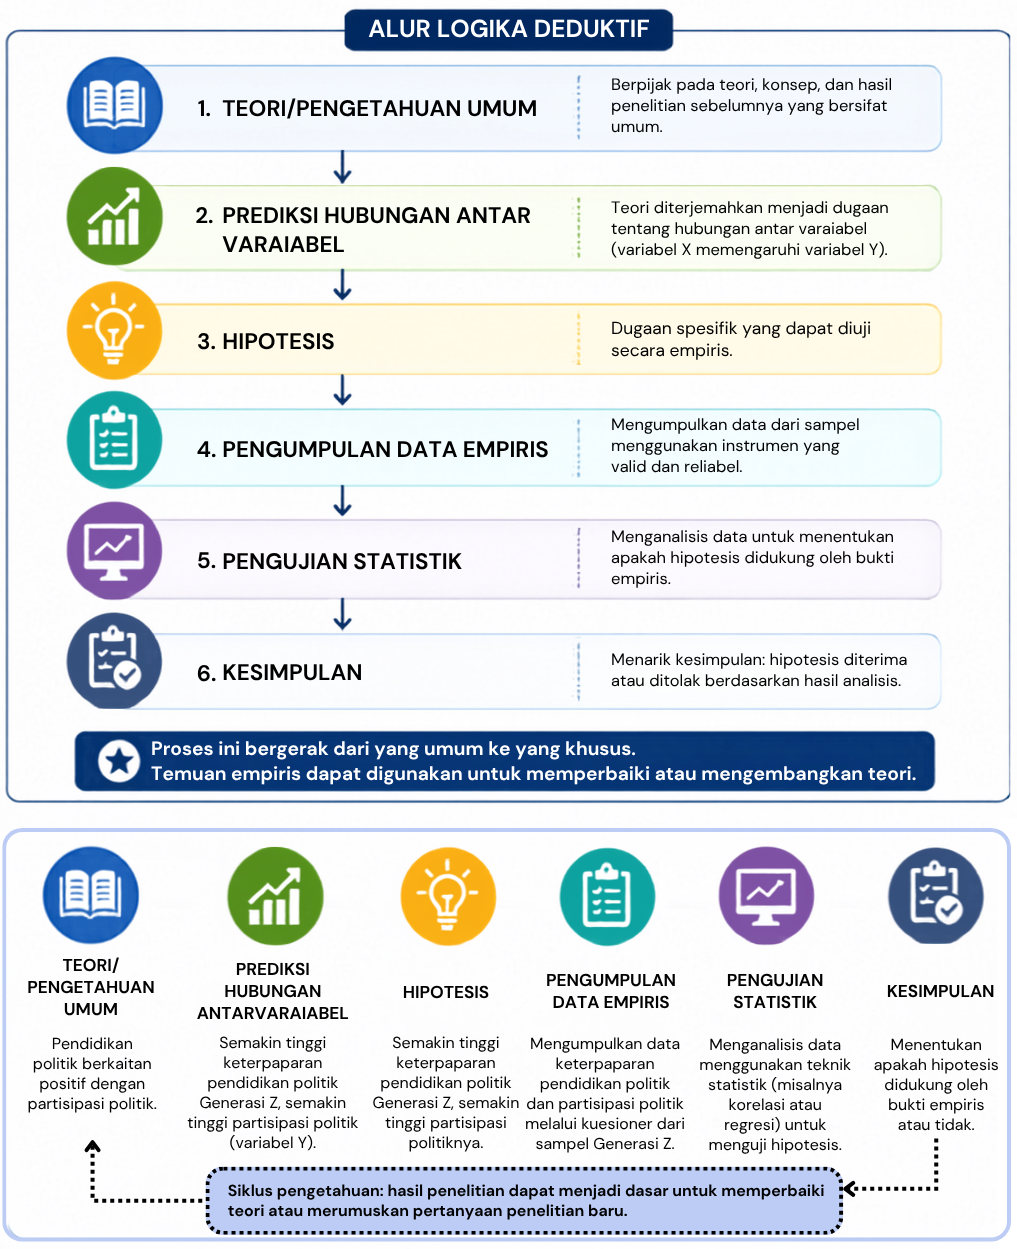
\includegraphics[keepaspectratio]{images/alurkuanti.png}}
\caption{Siklus Penelitian Kuantitatif}
\end{figure}

}

\caption{\label{fig-deduktif}}

\end{figure}%

Meskipun demikian, deduksi dan induksi tidak harus dipandang sebagai dua
proses yang sepenuhnya terpisah. Temuan empiris dari penelitian
kuantitatif dapat menghasilkan pola atau persoalan baru yang kemudian
digunakan untuk memperbaiki dan mengembangkan penjelasan teoretis.
Dengan demikian, perkembangan pengetahuan ilmiah berlangsung secara
berkelanjutan melalui hubungan antara teori dan bukti empiris (Babbie,
2021).

\section{Silogisme dalam Penelitian
Kuantitatif}\label{silogisme-dalam-penelitian-kuantitatif}

Logika deduktif berkaitan erat dengan silogisme, yaitu bentuk penalaran
yang menghasilkan kesimpulan berdasarkan premis-premis yang telah
ditetapkan. Dalam bentuk sederhana, silogisme terdiri atas premis mayor,
premis minor, dan kesimpulan. Jika premis yang digunakan benar dan
struktur penalarannya valid, kesimpulan yang dihasilkan mengikuti premis
tersebut secara logis (Cohen dkk., 2018; Smith dkk., 2022).

Sebagai contoh:

\begin{quote}
\textbf{Premis mayor}: Semua manusia akan mati.

\textbf{Premis minor:} Katrina adalah manusia.

\textbf{Kesimpulan}: Katrina akan mati.
\end{quote}

Dalam penelitian kuantitatif, pola penalaran tersebut membantu
menjelaskan bagaimana peneliti bergerak dari pengetahuan yang bersifat
umum menuju dugaan yang lebih spesifik. Teori dan temuan penelitian
sebelumnya menyediakan dasar penalaran, sedangkan kesimpulan yang
diturunkan darinya dapat menjadi dasar dalam merumuskan hipotesis yang
selanjutnya diuji menggunakan data empiris.

\subsection{Silogisme Kategoris}\label{silogisme-kategoris}

Silogisme kategoris merupakan penalaran yang premis dan kesimpulannya
berupa pernyataan tanpa syarat. Dalam penelitian, pola ini dapat
digunakan untuk menggambarkan bagaimana suatu pengetahuan umum
diterapkan pada kondisi yang lebih khusus.

Silogisme kategoris merupakan bentuk penalaran yang premis dan
kesimpulannya berupa pernyataan tanpa syarat. Silogisme ini terdiri atas
premis mayor yang memuat pernyataan umum, premis minor yang memuat
pernyataan lebih khusus, dan kesimpulan yang diturunkan dari kedua
premis tersebut.

Sebagai contoh, pertumbuhan tinggi badan yang cepat (\emph{growth
spurt}) merupakan salah satu karakteristik perkembangan fisik pada masa
pubertas. Penalarannya dapat disederhanakan sebagai berikut:

\begin{quote}
\textbf{Premis mayor}: Anak yang memasuki masa pubertas mengalami
\emph{growth spurt}.

\textbf{Premis minor}: Anak-anak usia awal belasan di daerah X sedang
memasuki masa pubertas.

\textbf{Prediksi}: Anak-anak usia awal belasan di daerah X akan
menunjukkan pertambahan tinggi badan yang cepat.
\end{quote}

Prediksi tersebut selanjutnya dapat diuji dengan melakukan pengukuran
tinggi badan secara berkala. Data yang diperoleh digunakan untuk menilai
apakah pola pertumbuhan yang diamati konsisten dengan prediksi yang
diturunkan dari pengetahuan sebelumnya.

\subsection{Silogisme Hipotetis}\label{silogisme-hipotetis}

Silogisme hipotetis menggunakan pernyataan bersyarat yang biasanya
berbentuk ``jika \ldots{} maka \ldots.'' Premis menyatakan bahwa suatu
kondisi akan menghasilkan konsekuensi tertentu. Bentuk penalaran ini
sangat relevan untuk menggambarkan hipotesis mengenai hubungan
sebab-akibat, khususnya dalam penelitian eksperimen.

Sebagai contoh, siswa mengeluh lebih cepat merasa lapar ketika belajar
di ruangan yang sangat dingin. Penalarannya dapat dirumuskan sebagai
berikut:

\begin{quote}
\textbf{Premis mayor}: Jika seseorang berada dalam ruangan yang sangat
dingin, maka ia akan lebih cepat merasa lapar.

\textbf{Premis minor}: Siswa ditempatkan dalam ruangan yang sangat
dingin.

\textbf{Prediksi}: Siswa yang berada dalam ruangan sangat dingin akan
lebih cepat merasa lapar dibandingkan siswa yang berada dalam ruangan
bersuhu normal.
\end{quote}

Prediksi tersebut dapat diuji dengan menempatkan dua kelompok siswa pada
kondisi yang sama, kecuali suhu ruangan. Waktu munculnya rasa lapar
kemudian dibandingkan antara kedua kelompok. Jika kelompok yang berada
dalam ruangan sangat dingin lebih cepat merasa lapar, data memberikan
dukungan terhadap prediksi yang diajukan.

Pemahaman terhadap logika deduktif menunjukkan bahwa hipotesis
penelitian bukan sekadar dugaan, melainkan prediksi yang memiliki dasar
teoretis dan dapat diuji secara empiris. Agar prediksi tersebut dapat
diuji, konsep-konsep yang terkandung di dalamnya perlu diterjemahkan
menjadi variabel yang dapat diamati dan diukur. Proses penyusunan
hipotesis dan operasionalisasi variabel inilah yang akan dibahas pada
bab berikutnya.

\begin{tcolorbox}[enhanced jigsaw, colframe=quarto-callout-tip-color-frame, toptitle=1mm, breakable, leftrule=.75mm, arc=.35mm, toprule=.15mm, colback=white, colbacktitle=quarto-callout-tip-color!10!white, bottomtitle=1mm, bottomrule=.15mm, titlerule=0mm, title=\textcolor{quarto-callout-tip-color}{\faLightbulb}\hspace{0.5em}{Rangkuman}, coltitle=black, left=2mm, opacitybacktitle=0.6, opacityback=0, rightrule=.15mm]

\begin{enumerate}
\def\labelenumi{\arabic{enumi}.}
\tightlist
\item
  Penelitian kuantitatif merupakan pendekatan yang menggunakan prosedur
  sistematis dan terstruktur untuk menguji teori atau hipotesis melalui
  pengukuran dan analisis data empiris.
\item
  Penelitian kuantitatif berakar pada filsafat positivisme yang
  memandang bahwa fenomena memiliki keteraturan serta dapat diamati,
  diukur, dan dipelajari menggunakan metode ilmiah.
\item
  Empat prinsip utama penelitian kuantitatif adalah \emph{determinism},
  \emph{empiricism}, \emph{parsimony}, dan \emph{generalization}.
  Prinsip-prinsip tersebut mendasari cara peneliti menjelaskan fenomena,
  melakukan pengukuran, membangun penjelasan, dan menarik kesimpulan.
\item
  Penelitian kuantitatif terutama menggunakan logika deduktif, yaitu
  penalaran yang bergerak dari teori atau pengetahuan yang bersifat umum
  menuju prediksi atau hipotesis yang lebih spesifik untuk kemudian
  diuji menggunakan data empiris.
\item
  Silogisme merupakan model sederhana untuk memahami penalaran deduktif.
  Silogisme kategoris bergerak dari pernyataan umum menuju kasus yang
  lebih khusus, sedangkan silogisme hipotetik menggunakan hubungan
  bersyarat dalam bentuk ``jika \ldots{} maka \ldots{}''.
\item
  Hasil penelitian tidak membuktikan suatu teori secara mutlak. Bukti
  empiris digunakan untuk menilai sejauh mana hasil penelitian konsisten
  atau tidak konsisten dengan prediksi yang diturunkan dari teori.
\end{enumerate}

\end{tcolorbox}

\begin{tcolorbox}[enhanced jigsaw, colframe=quarto-callout-important-color-frame, toptitle=1mm, breakable, leftrule=.75mm, arc=.35mm, toprule=.15mm, colback=white, colbacktitle=quarto-callout-important-color!10!white, bottomtitle=1mm, bottomrule=.15mm, titlerule=0mm, title=\textcolor{quarto-callout-important-color}{\faExclamation}\hspace{0.5em}{Refleksi \& Diskusi}, coltitle=black, left=2mm, opacitybacktitle=0.6, opacityback=0, rightrule=.15mm]

\begin{itemize}
\tightlist
\item
  Mengapa penelitian kuantitatif perlu dilakukan secara sistematis dan
  terstruktur? Kaitkan jawaban Anda dengan prinsip-prinsip penelitian
  kuantitatif.
\item
  Pilih satu fenomena psikologis yang menarik bagi Anda. Jelaskan
  bagaimana prinsip \emph{determinism}, \emph{empiricism},
  \emph{parsimony}, dan \emph{generalization} dapat diterapkan untuk
  meneliti fenomena tersebut.
\item
  Buatlah satu contoh sederhana yang menunjukkan alur teori → hipotesis
  → pengumpulan data → analisis → kesimpulan.
\item
  Mengapa hipotesis dalam penelitian kuantitatif seharusnya memiliki
  dasar teori atau temuan penelitian sebelumnya?
\item
  Seorang peneliti memperoleh hasil yang tidak mendukung hipotesisnya.
  Apakah hal tersebut berarti teori yang digunakannya pasti salah?
  Jelaskan alasan Anda.
\item
  Pilih salah satu topik penelitian, kemudian susun sebuah contoh
  silogisme kategoris atau hipotetik yang dapat menjadi dasar penalaran
  dalam penelitian tersebut.
\end{itemize}

\end{tcolorbox}

\phantomsection\label{refs--9}
\begin{CSLReferences}{1}{0}
\bibitem[\citeproctext]{ref-Babbie2021--9}
Babbie, E. (2021). \emph{The practice of social research} (15th ed.).
Cengage Learning.

\bibitem[\citeproctext]{ref-Cohen2108--9}
Cohen, L., Manion, L., \& Morrison, K. (2018). \emph{Research Methods in
Education} (8th ed.). Routledge.
\url{https://doi.org/10.4324/9781315456539}

\bibitem[\citeproctext]{ref-Creswell2018a--9}
Creswell, J. W., \& Creswell, J. D. (2023). \emph{Research design:
Qualitative, quantitative, and mixed methods approaches} (6th ed.). SAGE
Publications.

\bibitem[\citeproctext]{ref-Leavy2017--9}
Leavy, P. (2017). \emph{Research Design: Quantitative, Qualitative,
Mixed Methods, Arts-Based, and Community-Based Participatory Research
Approaches}. The Guilford Press.

\bibitem[\citeproctext]{ref-Neuman2014--9}
Neuman, W. L. (2014). \emph{Social research methods: Qualitative and
quantitative approaches} (7th ed.). Pearson.

\bibitem[\citeproctext]{ref-Smith2022--9}
Smith, J. A., Flowers, P., \& Larkin, M. (2022). \emph{Interpretative
Phenomenological Analysis: Theory, Method and Research} (2nd ed.). SAGE
Publications Ltd.

\end{CSLReferences}

\chapter{Hipotesis dan Operasionalisasi
Variabel}\label{hipotesis-dan-operasionalisasi-variabel}

\begin{tcolorbox}[enhanced jigsaw, colframe=quarto-callout-note-color-frame, toptitle=1mm, breakable, leftrule=.75mm, arc=.35mm, toprule=.15mm, colback=white, colbacktitle=quarto-callout-note-color!10!white, bottomtitle=1mm, bottomrule=.15mm, titlerule=0mm, title=\textcolor{quarto-callout-note-color}{\faInfo}\hspace{0.5em}{Capaian Pembelajaran}, coltitle=black, left=2mm, opacitybacktitle=0.6, opacityback=0, rightrule=.15mm]

Setelah mempelajari bab ini, mahasiswa diharapkan mampu:

\begin{enumerate}
\def\labelenumi{\arabic{enumi}.}
\tightlist
\item
  Menjelaskan konsep, fungsi, dan jenis-jenis hipotesis dalam
  penelitian.
\item
  Merumuskan hipotesis penelitian yang sesuai dengan tujuan, kerangka
  berpikir, dan desain penelitian.
\item
  Menjelaskan konsep variabel, definisi konseptual, dan definisi
  operasional.
\item
  Mengoperasionalkan variabel penelitian menjadi indikator yang dapat
  diukur.
\item
  Menyusun tabel operasionalisasi variabel sebagai dasar pengembangan
  instrumen penelitian.
\end{enumerate}

\end{tcolorbox}

Hipotesis dan operasionalisasi variabel merupakan bagian penting dari
proses penelitian kuantitatif karena keduanya memastikan bahwa
penelitian dilakukan secara sistematis, objektif, dan dapat diuji.
Hipotesis memberikan arah mengenai hubungan, perbedaan, atau pengaruh
yang ingin diuji, sedangkan operasionalisasi variabel menjelaskan
bagaimana setiap variabel didefinisikan dan diukur secara empiris.

Pada bab ini akan dibahas konsep dasar hipotesis, jenis-jenis hipotesis,
prinsip-prinsip penyusunannya, serta cara mengoperasionalkan variabel
penelitian ke dalam bentuk yang dapat diukur sebagai dasar penyusunan
instrumen penelitian.

\section{Hipotesis Penelitian}\label{hipotesis-penelitian}

Salah satu karakteristik utama penelitian kuantitatif adalah adanya
dugaan ilmiah yang akan diuji melalui pengumpulan dan analisis data.
Dugaan tersebut dikenal sebagai \textbf{hipotesis}. Hipotesis memberikan
arah yang jelas mengenai apa yang ingin dibuktikan atau diuji sehingga
seluruh proses penelitian, mulai dari pemilihan variabel, penyusunan
instrumen, pengumpulan data, hingga analisis statistik, dilakukan secara
sistematis dan terarah.

Hipotesis bukan sekadar dugaan atau perkiraan pribadi peneliti.
Hipotesis harus disusun berdasarkan landasan teori, hasil penelitian
terdahulu, maupun kerangka konseptual yang logis. Oleh karena itu,
hipotesis merupakan dugaan ilmiah (\emph{educated guess}) yang memiliki
dasar konseptual dan dapat diuji menggunakan metode ilmiah. Dalam
penelitian kuantitatif, kualitas hipotesis yang dirumuskan akan
menentukan ketepatan pemilihan desain penelitian, instrumen pengukuran,
teknik analisis statistik, serta interpretasi hasil penelitian.

\subsection{Pengertian Hipotesis}\label{pengertian-hipotesis}

Hipotesis merupakan dugaan atau jawaban sementara terhadap rumusan
masalah penelitian yang masih memerlukan pembuktian melalui pengumpulan
dan analisis data empiris. Disebut sebagai ``jawaban sementara'' karena
kebenarannya belum dapat dipastikan sebelum dilakukan pengujian
menggunakan metode ilmiah. Dalam literatur metodologi penelitian modern,
hipotesis dipandang sebagai prediksi yang dapat diuji secara empiris
mengenai hubungan, perbedaan, atau pengaruh antarvariabel. Hipotesis
disusun berdasarkan landasan teori, hasil penelitian terdahulu, serta
penalaran logis yang dikembangkan oleh peneliti, sehingga bukan sekadar
dugaan atau opini pribadi (Creswell \& Creswell, 2023; Gravetter \&
Forzano, 2018).

Dalam penelitian kuantitatif, hipotesis berfungsi sebagai dasar untuk
menentukan hubungan, perbedaan, atau pengaruh yang akan diuji.
Keberadaan hipotesis membantu peneliti menetapkan variabel penelitian,
memilih desain penelitian yang sesuai, menentukan teknik analisis
statistik, serta menginterpretasikan hasil penelitian secara objektif.
Dengan demikian, hipotesis menjadi salah satu komponen yang membedakan
penelitian kuantitatif inferensial dari penelitian yang hanya bersifat
deskriptif.

Perlu dipahami bahwa tidak semua penelitian kuantitatif memerlukan
hipotesis. Penelitian deskriptif yang bertujuan menggambarkan
karakteristik suatu populasi umumnya tidak mengajukan hipotesis karena
tidak berusaha menguji hubungan atau perbedaan antarvariabel.
Sebaliknya, penelitian korelasional, komparatif, eksperimen, maupun
penelitian yang menggunakan analisis regresi umumnya memerlukan
hipotesis sebagai dasar pengujian empiris.

Contoh:

\begin{quote}
\textbf{Rumusan masalah:} Apakah terdapat hubungan antara resiliensi dan
\emph{academic burnout} pada mahasiswa?

\textbf{Hipotesis penelitian:} Terdapat hubungan negatif antara
resiliensi dan \emph{academic burnout} pada mahasiswa.
\end{quote}

\subsection{Klasifikasi Hipotesis}\label{klasifikasi-hipotesis}

Hipotesis dapat diklasifikasikan berdasarkan beberapa sudut pandang.
Dalam penelitian kuantitatif, klasifikasi yang paling umum didasarkan
pada fungsi hipotesis dalam penelitian, bentuk statistik yang digunakan
dalam pengujian, serta arah dugaan yang diajukan peneliti (Creswell \&
Creswell, 2023; Gravetter \& Forzano, 2018). Memahami berbagai jenis
hipotesis ini penting karena setiap jenis memiliki tujuan dan cara
perumusan yang berbeda sesuai dengan desain penelitian dan teknik
analisis statistik yang digunakan.

\begin{enumerate}
\def\labelenumi{\arabic{enumi}.}
\item
  \textbf{Berdasarkan Fungsinya dalam Penelitian}

  Berdasarkan fungsinya, hipotesis dibedakan menjadi \textbf{hipotesis
  penelitian (\emph{research hypothesis})} dan \textbf{hipotesis
  statistik (\emph{statistical hypothesis})}. Hipotesis penelitian
  merupakan dugaan ilmiah yang dirumuskan berdasarkan teori, hasil
  penelitian terdahulu, serta kerangka berpikir peneliti. Hipotesis ini
  ditulis dalam bentuk kalimat substantif yang menjelaskan adanya
  hubungan, perbedaan, atau pengaruh antarvariabel, tanpa menggunakan
  simbol atau notasi statistik (Creswell \& Creswell, 2023). Hipotesis
  penelitian inilah yang biasanya dituliskan pada proposal atau laporan
  penelitian sebagai jawaban sementara terhadap rumusan masalah.

  Contoh:

  \begin{quote}
  Terdapat hubungan positif antara \emph{self-efficacy} dan motivasi
  belajar mahasiswa.
  \end{quote}

  atau

  \begin{quote}
  Pelatihan \emph{mindfulness} menurunkan tingkat stres mahasiswa.
  \end{quote}

  Ketika data penelitian akan dianalisis menggunakan statistik
  inferensial, hipotesis penelitian diterjemahkan ke dalam bentuk
  hipotesis statistik. Hipotesis statistik menggunakan simbol matematis
  atau notasi statistik sehingga dapat diuji melalui prosedur analisis
  statistik (Gravetter \& Forzano, 2018).
\item
  \textbf{Berdasarkan Bentuk Statistik}

  Hipotesis statistik terdiri atas dua bentuk, yaitu \textbf{hipotesis
  nol (H₀)} dan \textbf{hipotesis alternatif (H₁ atau Hₐ)}. Hipotesis
  nol menyatakan bahwa \textbf{tidak terdapat hubungan, tidak terdapat
  perbedaan, atau tidak terdapat pengaruh} antarvariabel dalam populasi.
  Dengan kata lain, setiap perbedaan atau hubungan yang ditemukan pada
  sampel dianggap tidak cukup kuat untuk menyimpulkan adanya hubungan
  atau perbedaan dalam populasi (Gravetter \& Forzano, 2018).

  Contoh:

  \begin{quote}
  H₀: Tidak terdapat hubungan antara \emph{self-efficacy} dan motivasi
  belajar mahasiswa.
  \end{quote}

  atau

  \begin{quote}
  H₀: Tidak terdapat perbedaan tingkat stres antara kelompok yang
  mengikuti pelatihan \emph{mindfulness} dan kelompok kontrol.
  \end{quote}

  Dalam praktik penelitian, pengujian statistik pada dasarnya dilakukan
  untuk mengevaluasi apakah terdapat bukti yang cukup untuk
  \textbf{menolak H₀}. Oleh karena itu, peneliti tidak berusaha
  ``membuktikan'' H₀ benar, melainkan mencari bukti apakah H₀ dapat
  ditolak berdasarkan data yang diperoleh.

  Hipotesis alternatif merupakan kebalikan dari hipotesis nol. Hipotesis
  ini menyatakan bahwa \textbf{terdapat hubungan, perbedaan, atau
  pengaruh} antarvariabel dalam populasi. Dalam laporan penelitian,
  hipotesis penelitian yang ditulis pada Bab Pendahuluan umumnya
  merupakan bentuk verbal dari hipotesis alternatif, sedangkan H₀ dan H₁
  digunakan secara eksplisit pada tahap analisis statistik.

  Contoh:

  \begin{quote}
  H₁: Terdapat hubungan antara \emph{self-efficacy} dan motivasi belajar
  mahasiswa.
  \end{quote}

  atau

  \begin{quote}
  H₁: Terdapat perbedaan tingkat stres antara kelompok yang mengikuti
  pelatihan \emph{mindfulness} dan kelompok kontrol.
  \end{quote}
\item
  \textbf{Berdasarkan Arah Dugaan}

  Berdasarkan arah dugaan yang diajukan, hipotesis alternatif dibedakan
  menjadi \textbf{hipotesis satu arah (\emph{directional/one-tailed
  hypothesis})} dan \textbf{hipotesis dua arah
  (\emph{non-directional/two-tailed hypothesis})} (Creswell \& Creswell,
  2023). Hipotesis satu arah digunakan apabila teori atau hasil
  penelitian sebelumnya (bukti empiris) memberikan dasar yang kuat
  mengenai arah hubungan, perbedaan, atau pengaruh yang diharapkan.

  Contoh:

  \begin{quote}
  Terdapat hubungan positif antara \emph{self-efficacy} dan motivasi
  belajar mahasiswa.
  \end{quote}

  atau

  \begin{quote}
  Mahasiswa yang mengikuti pelatihan \emph{mindfulness} memiliki tingkat
  stres yang lebih rendah dibandingkan mahasiswa yang tidak mengikuti
  pelatihan.
  \end{quote}

  Pada contoh tersebut, arah dugaan telah ditentukan sejak awal, yaitu
  \emph{positif} atau \emph{lebih rendah}.

  Hipotesis dua arah digunakan apabila peneliti hanya menduga adanya
  hubungan, perbedaan, atau pengaruh tanpa menentukan arahnya. Hipotesis
  ini biasanya digunakan ketika bukti teoritis maupun hasil penelitian
  sebelumnya belum cukup kuat untuk memprediksi arah hubungan.

  Contoh:

  \begin{quote}
  Terdapat hubungan antara \emph{self-efficacy} dan motivasi belajar
  mahasiswa.
  \end{quote}

  atau

  \begin{quote}
  Terdapat perbedaan tingkat stres antara mahasiswa yang mengikuti
  pelatihan \emph{mindfulness} dan mahasiswa yang tidak mengikuti
  pelatihan.
  \end{quote}

  Pada hipotesis ini, peneliti tidak menyatakan apakah hubungan tersebut
  positif atau negatif, maupun kelompok mana yang diperkirakan memiliki
  skor lebih tinggi.
\end{enumerate}

\subsection{Karakteristik Hipotesis yang
Baik}\label{karakteristik-hipotesis-yang-baik}

Hipotesis merupakan dugaan ilmiah yang menjadi dasar pengujian dalam
penelitian kuantitatif. Agar dapat berfungsi sebagai pedoman penelitian
sekaligus dapat diuji secara empiris, hipotesis perlu memenuhi sejumlah
karakteristik tertentu. Meskipun setiap buku metodologi penelitian
menggunakan istilah yang sedikit berbeda, secara umum hipotesis yang
baik memiliki enam karakteristik berikut (Creswell \& Creswell, 2023;
Gravetter \& Forzano, 2018; Kerlinger \& Lee, 2000; Neuman, 2014):

\begin{enumerate}
\def\labelenumi{\arabic{enumi}.}
\item
  \textbf{Berdasarkan teori dan bukti empiris}

  Hipotesis tidak disusun berdasarkan intuisi atau dugaan pribadi
  peneliti. Sebaliknya, hipotesis harus berangkat dari teori yang
  relevan, hasil penelitian terdahulu, maupun kerangka konseptual yang
  logis. Dengan demikian, hipotesis memiliki landasan ilmiah yang kuat
  dan dapat dipertanggungjawabkan.
\item
  \textbf{Dirumuskan secara jelas dan spesifik}

  Hipotesis harus menggunakan kalimat yang jelas sehingga tidak
  menimbulkan penafsiran yang berbeda. Selain itu, variabel yang
  diteliti harus disebutkan secara spesifik sehingga pembaca memahami
  apa yang akan diuji.

  \emph{Kurang tepat}:

  \begin{quote}
  Stres memengaruhi kehidupan mahasiswa.
  \end{quote}

  \emph{Lebih tepat}:

  \begin{quote}
  Tingkat stres akademik berhubungan negatif dengan kesejahteraan
  psikologis mahasiswa.
  \end{quote}
\item
  \textbf{Menyatakan hubungan antarvariabel}

  Dalam penelitian kuantitatif, hipotesis harus menjelaskan hubungan,
  perbedaan, atau pengaruh antarvariabel. Dengan kata lain, hipotesis
  harus menunjukkan dengan jelas variabel mana yang menjadi prediktor,
  variabel yang diprediksi, atau kelompok yang dibandingkan.
\item
  \textbf{Dapat diuji secara empiris}

  Hipotesis harus berkaitan dengan variabel yang dapat diamati atau
  diukur sehingga dapat diuji menggunakan data empiris. Apabila suatu
  konsep tidak dapat diukur melalui indikator yang jelas, maka hipotesis
  tersebut tidak dapat diuji secara ilmiah.
\item
  \textbf{Dapat dibuktikan salah (\emph{falsifiable})}

  Menurut Popper (2005), suatu hipotesis ilmiah harus memungkinkan untuk
  dibuktikan salah apabila data empiris tidak mendukungnya. Oleh karena
  itu, hipotesis tidak boleh berupa pernyataan yang selalu dianggap
  benar dalam segala situasi. Sebagai contoh, hipotesis ``Semua
  mahasiswa selalu belajar dengan sungguh-sungguh'' bukan merupakan
  hipotesis ilmiah yang baik karena sulit dirumuskan dalam bentuk yang
  dapat diuji secara objektif.
\item
  \textbf{Konsisten dengan tujuan penelitian}

  Hipotesis harus sesuai dengan tujuan penelitian dan desain penelitian
  yang digunakan. Penelitian korelasional, misalnya, seharusnya
  merumuskan hipotesis mengenai hubungan antarvariabel, sedangkan
  penelitian eksperimen merumuskan hipotesis mengenai pengaruh suatu
  perlakuan terhadap variabel tertentu.
\end{enumerate}

Gambar~\ref{fig-hipotesis} mengilustrasikan bagaimana proses perumusan
hipotesis dalam 3 desain penelitian yang berbeda.

\begin{figure}

\centering{

\begin{figure}
\centering
\pandocbounded{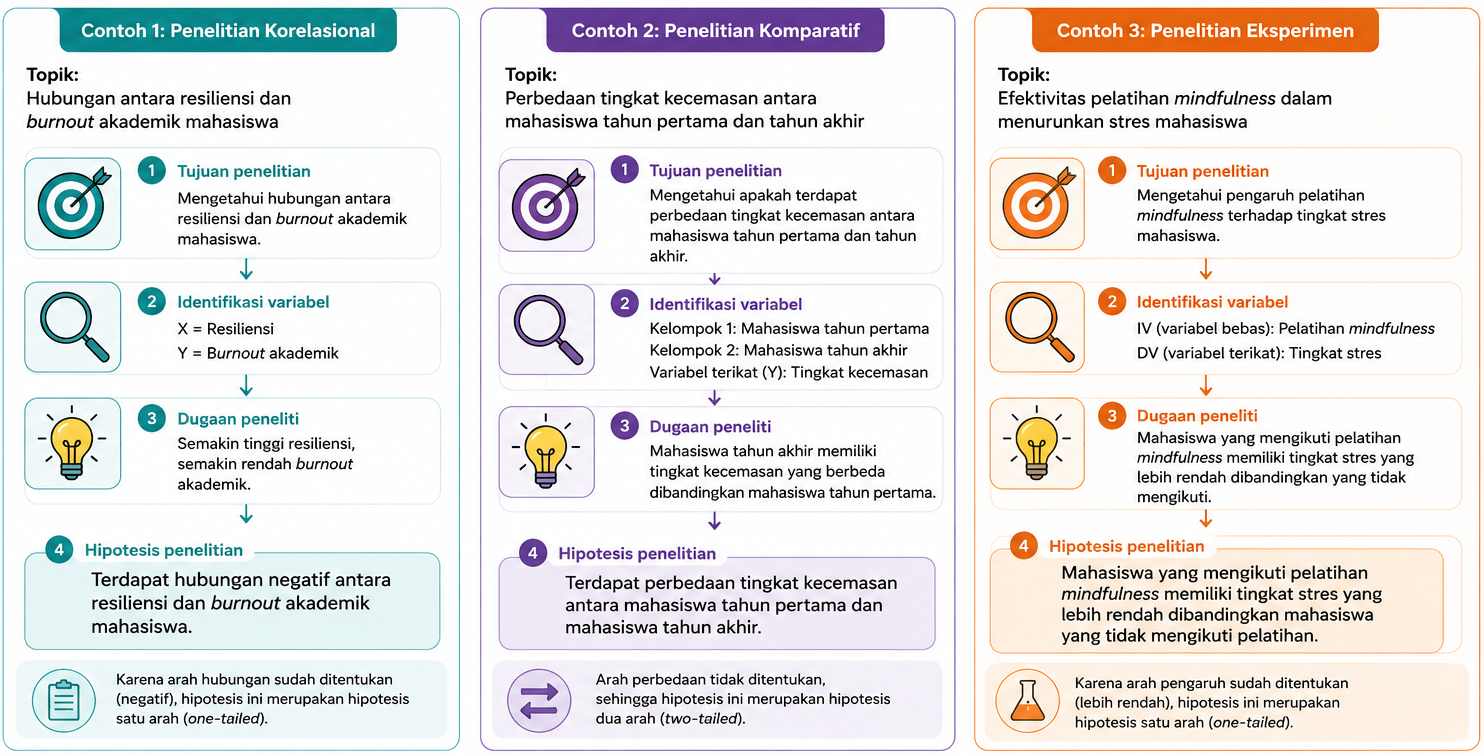
\includegraphics[keepaspectratio]{images/hipotesis.png}}
\caption{Contoh Proses Perumusan Hipotesis}
\end{figure}

}

\caption{\label{fig-hipotesis}}

\end{figure}%

\begin{tcolorbox}[enhanced jigsaw, colframe=quarto-callout-tip-color-frame, toptitle=1mm, breakable, leftrule=.75mm, arc=.35mm, toprule=.15mm, colback=white, colbacktitle=quarto-callout-tip-color!10!white, bottomtitle=1mm, bottomrule=.15mm, titlerule=0mm, title={Kesalahan yang Sering Terjadi dalam Merumuskan Hipotesis}, coltitle=black, left=2mm, opacitybacktitle=0.6, opacityback=0, rightrule=.15mm]

Mahasiswa sering melakukan beberapa kesalahan berikut ketika menyusun
hipotesis penelitian:

\begin{itemize}
\tightlist
\item
  Menyusun hipotesis tanpa didukung teori atau hasil penelitian
  terdahulu.
\item
  Merumuskan hipotesis yang terlalu umum sehingga variabel yang diteliti
  tidak jelas.
\item
  Menggunakan bentuk hipotesis yang tidak sesuai dengan tujuan
  penelitian, misalnya tujuan penelitian menguji hubungan tetapi
  hipotesis menyatakan adanya pengaruh.
\item
  Menggunakan konsep yang tidak dapat diukur secara empiris.
\item
  Menyusun hipotesis setelah melihat hasil analisis data (\emph{HARKing}
  atau \emph{Hypothesizing After the Results are Known}), padahal
  hipotesis seharusnya dirumuskan sebelum pengumpulan data dilakukan.
\end{itemize}

\end{tcolorbox}

\section{Operasionalisasi Variabel}\label{operasionalisasi-variabel}

Variabel merupakan konsep utama yang menjadi objek pengamatan dalam
penelitian kuantitatif. Namun, banyak variabel dalam ilmu sosial dan
psikologi, seperti \emph{resiliensi}, \emph{motivasi belajar},
\emph{burnout}, atau \emph{kesejahteraan psikologis}, tidak dapat
diamati secara langsung. Konsep-konsep tersebut bersifat abstrak
sehingga perlu diterjemahkan ke dalam bentuk yang dapat diamati dan
diukur melalui proses \textbf{operasionalisasi variabel}.

Operasionalisasi variabel merupakan langkah penting dalam penelitian
kuantitatif karena menentukan bagaimana suatu konsep akan diukur secara
empiris. Proses ini mencakup penetapan definisi operasional, pemilihan
indikator, penentuan instrumen pengukuran, hingga cara pemberian skor
terhadap data yang diperoleh. Operasionalisasi yang baik memastikan
bahwa data yang dikumpulkan benar-benar merepresentasikan konsep yang
ingin diteliti sehingga hasil penelitian menjadi lebih valid dan
reliabel (Creswell \& Creswell, 2023; Kerlinger \& Lee, 2000).

\subsection{Apa Itu Operasionalisasi
Variabel?}\label{apa-itu-operasionalisasi-variabel}

Operasionalisasi variabel adalah proses mengubah konsep atau konstruk
teoretis menjadi variabel yang dapat diukur secara empiris melalui
indikator, instrumen pengukuran, prosedur penskoran, dan interpretasi
hasil pengukuran (Creswell \& Creswell, 2023; Kerlinger \& Lee, 2000).
Dengan kata lain, operasionalisasi menjelaskan bagaimana suatu konsep
akan diukur dalam penelitian (lihat Gambar~\ref{fig-operasionalisasi}).

Sebagai contoh, apabila seorang peneliti ingin mengukur
\emph{resiliensi}, ia tidak cukup hanya menyebutkan definisi resiliensi
menurut teori tertentu. Peneliti juga harus menjelaskan instrumen yang
digunakan, dimensi atau indikator yang diukur, cara pemberian skor,
serta makna dari skor yang diperoleh. Melalui operasionalisasi, konsep
yang semula bersifat abstrak dapat diubah menjadi data numerik yang
selanjutnya dianalisis menggunakan teknik statistik.

Operasionalisasi variabel merupakan salah satu tahapan penting dalam
penelitian kuantitatif karena menentukan kualitas data yang diperoleh.
Operasionalisasi yang kurang tepat dapat menyebabkan instrumen gagal
merepresentasikan konsep yang ingin diukur sehingga hasil penelitian
menjadi kurang valid. Sebaliknya, operasionalisasi yang baik akan
menghasilkan pengukuran yang lebih akurat, konsisten, dan sesuai dengan
tujuan penelitian (DeVellis \& Thorpe, 2023).

\begin{figure}

\centering{

\begin{figure}
\centering
\pandocbounded{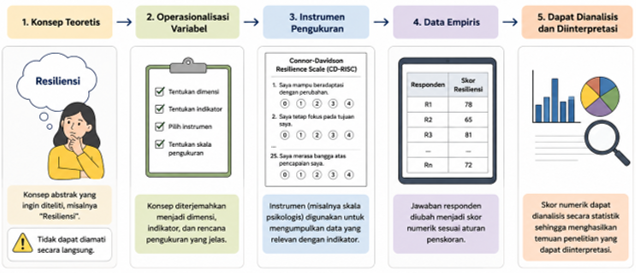
\includegraphics[keepaspectratio]{images/operasionalisasi.png}}
\caption{Pentingnya Operasionalisasi Variabel Penelitian}
\end{figure}

}

\caption{\label{fig-operasionalisasi}}

\end{figure}%

\subsection{Definisi Konseptual dan Definisi
Operasional}\label{definisi-konseptual-dan-definisi-operasional}

Dalam proses operasionalisasi, peneliti perlu membedakan
\textbf{definisi konseptual} dan \textbf{definisi operasional}. Kedua
jenis definisi tersebut saling melengkapi, tetapi memiliki tujuan yang
berbeda.

Definisi konseptual menjelaskan makna suatu konsep atau konstruk
berdasarkan teori maupun kajian ilmiah sehingga memberikan batasan yang
jelas mengenai apa yang dimaksud dengan variabel penelitian (Babbie,
2021; Creswell \& Creswell, 2023). Definisi ini bertujuan memberikan
batasan ilmiah mengenai konsep yang diteliti sehingga pembaca memahami
ruang lingkup variabel penelitian. Oleh karena itu, definisi konseptual
biasanya disusun berdasarkan kajian literatur dan mengacu pada teori
yang menjadi landasan penelitian.

Sebaliknya, Definisi operasional menjelaskan bagaimana konsep tersebut
diukur melalui prosedur empiris, termasuk indikator, instrumen, skala
pengukuran, dan prosedur penskoran yang digunakan dalam penelitian.
Dengan demikian, definisi operasional menjembatani konsep teoretis
dengan proses pengumpulan data empiris (American Psychological
Association, 2018; Kerlinger \& Lee, 2000). Perbedaan kedua jenis
definisi tersebut dapat dilihat pada Tabel~\ref{tbl-definisi}.

Sebagai ilustrasi, konsep \emph{resiliensi} dapat didefinisikan secara
konseptual sebagai kemampuan individu untuk beradaptasi secara positif
ketika menghadapi kesulitan atau tekanan hidup. Namun, dalam penelitian,
konsep tersebut perlu didefinisikan secara operasional, misalnya sebagai
skor yang diperoleh responden pada \emph{Connor--Davidson Resilience
Scale} (CD-RISC-10). Semakin tinggi skor yang diperoleh, semakin tinggi
tingkat resiliensi individu.

\begin{longtable}[]{@{}
  >{\raggedright\arraybackslash}p{(\linewidth - 4\tabcolsep) * \real{0.3333}}
  >{\raggedright\arraybackslash}p{(\linewidth - 4\tabcolsep) * \real{0.3333}}
  >{\raggedright\arraybackslash}p{(\linewidth - 4\tabcolsep) * \real{0.3333}}@{}}
\caption{Perbedaan Definisi Konseptual dan Definisi
Operasional}\label{tbl-definisi}\tabularnewline
\toprule\noalign{}
\endfirsthead
\endhead
\bottomrule\noalign{}
\endlastfoot
\textbf{Aspek} & \textbf{Definisi Konseptual} & \textbf{Definisi
Operasional} \\
Tujuan & Menjelaskan makna suatu konsep berdasarkan teori & Menjelaskan
bagaimana konsep diukur dalam penelitian \\
Sumber & Teori dan kajian literatur & Instrumen dan prosedur
pengukuran \\
Fokus & Makna atau hakikat konsep & Pengukuran empiris \\
Isi & Definisi dari ahli, karakteristik konsep & Instrumen, indikator,
skala, penskoran, interpretasi \\
\end{longtable}

Definisi konseptual dan definisi operasional harus disusun secara
selaras karena definisi operasional merupakan penerjemahan dari konsep
teoretis ke dalam bentuk yang dapat diukur secara empiris. Oleh karena
itu, menurut Babbie (2021), indikator, dimensi, maupun instrumen yang
digunakan harus benar-benar merepresentasikan konstruk yang telah
didefinisikan secara konseptual. Keselarasan ini penting untuk
memastikan bahwa data yang dikumpulkan benar-benar mengukur variabel
yang dimaksud sehingga menghasilkan temuan penelitian yang valid dan
dapat dipertanggungjawabkan (AERA, APA, \& NCME, 2014; DeVellis \&
Thorpe, 2023).

\begin{tcolorbox}[enhanced jigsaw, colframe=quarto-callout-tip-color-frame, toptitle=1mm, breakable, leftrule=.75mm, arc=.35mm, toprule=.15mm, colback=white, colbacktitle=quarto-callout-tip-color!10!white, bottomtitle=1mm, bottomrule=.15mm, titlerule=0mm, title={Contoh Operasionalisasi Variabel}, coltitle=black, left=2mm, opacitybacktitle=0.6, opacityback=0, rightrule=.15mm]

\textbf{Variabel:} \emph{Academic burnout}

\textbf{Definisi konseptual:} \emph{Academic burnout} merupakan kondisi
kelelahan fisik, emosional, dan mental akibat tuntutan akademik yang
berkepanjangan (Schaufeli dkk., 2002).

\textbf{Definisi operasional:} \emph{Academic burnout} diukur
menggunakan \textbf{\emph{Maslach Burnout Inventory--Student Survey}}
\textbf{(MBI-SS)} yang dikembangkan oleh Schaufeli dkk. (2002). Alat
ukur ini terdiri atas tiga dimensi, yaitu \emph{exhaustion},
\emph{cynicism}, dan \emph{academic efficacy}. Semakin tinggi skor pada
dimensi \emph{exhaustion} dan \emph{cynicism} serta semakin rendah skor
\emph{academic efficacy}, semakin tinggi tingkat \emph{academic
burnout}.

\end{tcolorbox}

\subsection{Mengoperasionalkan Variabel
Penelitian}\label{mengoperasionalkan-variabel-penelitian}

Operasionalisasi variabel merupakan proses sistematis yang menghubungkan
konsep teoretis dengan pengukuran empiris. Dalam praktiknya, proses ini
tidak hanya menentukan instrumen yang akan digunakan, tetapi juga
memastikan bahwa setiap aspek yang diukur benar-benar merepresentasikan
konstruk yang menjadi fokus penelitian. Secara umum, operasionalisasi
variabel dapat dilakukan melalui lima langkah berikut:

\begin{enumerate}
\def\labelenumi{\arabic{enumi}.}
\item
  \textbf{Menentukan konsep atau konstruk yang akan diukur}

  Langkah pertama adalah menetapkan secara jelas konsep yang menjadi
  variabel penelitian. Konsep tersebut harus didefinisikan berdasarkan
  teori yang menjadi landasan penelitian sehingga memiliki batasan yang
  jelas.

  Sebagai contoh, apabila variabel yang diteliti adalah
  \emph{resiliensi}, peneliti terlebih dahulu menentukan definisi
  konseptual yang akan digunakan, misalnya berdasarkan teori Connor dan
  Davidson.
\item
  \textbf{Mengidentifikasi dimensi atau indikator variabel}

  Sebagian besar konstruk psikologis bersifat multidimensional. Oleh
  karena itu, setelah menentukan definisi konseptual, peneliti perlu
  mengidentifikasi dimensi atau indikator yang menyusun variabel
  tersebut berdasarkan teori atau instrumen yang digunakan.

  Sebagai contoh, apabila menggunakan \emph{Connor--Davidson Resilience
  Scale (CD-RISC)}, maka indikator yang diukur mengikuti dimensi yang
  dikembangkan oleh penyusun instrumen tersebut.
\item
  \textbf{Menentukan instrumen pengukuran}

  Langkah berikutnya adalah memilih atau mengembangkan instrumen yang
  sesuai dengan konstruk yang akan diukur. Dalam penelitian kuantitatif,
  peneliti umumnya menggunakan instrumen yang telah memiliki bukti
  validitas dan reliabilitas sehingga hasil pengukuran lebih dapat
  dipercaya (DeVellis \& Thorpe, 2023).

  Apabila menggunakan instrumen yang telah ada, peneliti perlu
  menjelaskan nama instrumen, jumlah item, dimensi yang diukur, jenis
  skala, serta bukti validitas dan reliabilitasnya. Sebaliknya, apabila
  mengembangkan instrumen sendiri, peneliti perlu menjelaskan proses
  pengembangan instrumen tersebut secara rinci.
\item
  \textbf{Menentukan prosedur penskoran}

  Operasionalisasi variabel juga harus menjelaskan bagaimana jawaban
  responden diubah menjadi skor numerik. Peneliti perlu menjelaskan
  jenis skala yang digunakan (misalnya skala Likert 1--5), cara
  menghitung skor total atau skor setiap dimensi, serta perlakuan
  terhadap item yang bersifat \emph{reverse} apabila ada.
\item
  \textbf{Menentukan interpretasi hasil pengukuran}

  Langkah terakhir adalah menjelaskan makna skor yang diperoleh.
  Misalnya, apakah skor yang lebih tinggi menunjukkan tingkat variabel
  yang lebih tinggi atau justru sebaliknya. Penjelasan ini penting agar
  pembaca memahami bagaimana hasil pengukuran akan diinterpretasikan
  pada tahap analisis data.
\end{enumerate}

\begin{tcolorbox}[enhanced jigsaw, colframe=quarto-callout-tip-color-frame, toptitle=1mm, breakable, leftrule=.75mm, arc=.35mm, toprule=.15mm, colback=white, colbacktitle=quarto-callout-tip-color!10!white, bottomtitle=1mm, bottomrule=.15mm, titlerule=0mm, title={Kesalahan yang Sering Terjadi dalam Operasionalisasi Variabel}, coltitle=black, left=2mm, opacitybacktitle=0.6, opacityback=0, rightrule=.15mm]

Beberapa kesalahan yang sering dilakukan mahasiswa ketika menyusun
operasionalisasi variabel antara lain:

\begin{itemize}
\tightlist
\item
  Menyalin definisi konseptual sebagai definisi operasional tanpa
  menjelaskan cara pengukurannya.
\item
  Menggunakan instrumen yang tidak sesuai dengan definisi konseptual
  variabel.
\item
  Mencantumkan indikator yang tidak berasal dari teori atau instrumen
  yang digunakan.
\item
  Tidak menjelaskan prosedur penskoran maupun interpretasi skor.
\item
  Menggabungkan indikator dari beberapa teori tanpa dasar konseptual
  yang jelas.
\end{itemize}

\end{tcolorbox}

Setelah variabel berhasil dioperasionalkan, informasi tersebut biasanya
dirangkum dalam bentuk tabel operasionalisasi variabel. Tabel ini
berfungsi sebagai ringkasan mengenai bagaimana setiap variabel
didefinisikan dan diukur sehingga memudahkan pembaca memahami
keterkaitan antara konsep teoretis dan prosedur pengukuran. Contoh
format tabel operasionalisasi variabel disajikan pada
Tabel~\ref{tbl-operasionalisasi}.

\begin{longtable}[]{@{}
  >{\raggedright\arraybackslash}p{(\linewidth - 8\tabcolsep) * \real{0.2000}}
  >{\raggedright\arraybackslash}p{(\linewidth - 8\tabcolsep) * \real{0.2000}}
  >{\raggedright\arraybackslash}p{(\linewidth - 8\tabcolsep) * \real{0.2000}}
  >{\raggedright\arraybackslash}p{(\linewidth - 8\tabcolsep) * \real{0.2000}}
  >{\raggedright\arraybackslash}p{(\linewidth - 8\tabcolsep) * \real{0.2000}}@{}}
\caption{Contoh Tabel Operasionalisasi
Variabel}\label{tbl-operasionalisasi}\tabularnewline
\toprule\noalign{}
\endfirsthead
\endhead
\bottomrule\noalign{}
\endlastfoot
\textbf{Variabel} & \textbf{Definisi Konseptual} &
\textbf{Dimensi/Indikator} & \textbf{Instrumen} & \textbf{Skala} \\
\emph{Resiliensi} & Kemampuan individu untuk beradaptasi secara positif
ketika menghadapi kesulitan hidup. & Kemampuan beradaptasi, ketekunan,
regulasi emosi, optimisme & CD-RISC-10 & Likert 0--4 \\
\emph{Academic Burnout} & Kondisi kelelahan akibat tuntutan akademik
yang berkepanjangan. & \emph{Exhaustion}, \emph{cynicism},
\emph{academic efficacy} & MBI-SS & Likert 1--7 \\
\end{longtable}

\begin{tcolorbox}[enhanced jigsaw, colframe=quarto-callout-tip-color-frame, toptitle=1mm, breakable, leftrule=.75mm, arc=.35mm, toprule=.15mm, colback=white, colbacktitle=quarto-callout-tip-color!10!white, bottomtitle=1mm, bottomrule=.15mm, titlerule=0mm, title=\textcolor{quarto-callout-tip-color}{\faLightbulb}\hspace{0.5em}{Rangkuman}, coltitle=black, left=2mm, opacitybacktitle=0.6, opacityback=0, rightrule=.15mm]

\begin{enumerate}
\def\labelenumi{\arabic{enumi}.}
\tightlist
\item
  Hipotesis merupakan dugaan ilmiah yang disusun berdasarkan teori dan
  temuan penelitian terdahulu serta dapat diuji secara empiris untuk
  menjawab rumusan masalah penelitian.
\item
  Hipotesis dapat diklasifikasikan berdasarkan fungsinya dalam
  penelitian, bentuk statistiknya, dan arah dugaan yang diajukan
  peneliti. Pemilihan jenis hipotesis harus disesuaikan dengan tujuan
  penelitian dan teknik analisis yang akan digunakan.
\item
  Hipotesis yang baik harus memiliki landasan teoretis yang kuat,
  dirumuskan secara jelas dan spesifik, menyatakan hubungan
  antarvariabel, dapat diuji secara empiris, dapat dibuktikan salah
  (\emph{falsifiable}), serta konsisten dengan tujuan penelitian.
\item
  Operasionalisasi variabel merupakan proses menerjemahkan konsep atau
  konstruk teoretis menjadi variabel yang dapat diukur melalui
  indikator, instrumen, prosedur penskoran, dan interpretasi hasil
  pengukuran.
\item
  Definisi konseptual dan definisi operasional harus disusun secara
  selaras agar instrumen yang digunakan benar-benar mengukur konstruk
  yang menjadi fokus penelitian.
\item
  Hasil operasionalisasi variabel umumnya dirangkum dalam tabel
  operasionalisasi variabel yang menjadi dasar penyusunan instrumen dan
  pelaksanaan penelitian
\end{enumerate}

\end{tcolorbox}

\begin{tcolorbox}[enhanced jigsaw, colframe=quarto-callout-important-color-frame, toptitle=1mm, breakable, leftrule=.75mm, arc=.35mm, toprule=.15mm, colback=white, colbacktitle=quarto-callout-important-color!10!white, bottomtitle=1mm, bottomrule=.15mm, titlerule=0mm, title=\textcolor{quarto-callout-important-color}{\faExclamation}\hspace{0.5em}{Refleksi \& Diskusi}, coltitle=black, left=2mm, opacitybacktitle=0.6, opacityback=0, rightrule=.15mm]

\begin{enumerate}
\def\labelenumi{\arabic{enumi}.}
\item
  Mengapa penelitian kuantitatif yang bertujuan menguji hubungan,
  perbedaan, atau pengaruh antarvariabel umumnya memerlukan hipotesis,
  sedangkan penelitian deskriptif tidak selalu memerlukannya?
\item
  Perhatikan topik penelitian berikut:

  \begin{quote}
  \emph{Hubungan antara penggunaan media sosial dan kesejahteraan
  psikologis pada mahasiswa.}
  \end{quote}

  Lakukan langkah-langkah berikut:

  \begin{itemize}
  \tightlist
  \item
    Rumuskan satu hipotesis penelitian.
  \item
    Tentukan hipotesis nol (H₀) dan hipotesis alternatif (H₁).
  \item
    Jelaskan apakah hipotesis tersebut termasuk hipotesis satu arah atau
    dua arah beserta alasannya.
  \end{itemize}
\item
  Pilih satu variabel psikologis yang Anda minati (misalnya
  \emph{resiliensi}, \emph{self-esteem}, \emph{academic burnout}, atau
  \emph{motivasi belajar}), kemudian lakukan operasionalisasi variabel
  dengan mengidentifikasi:

  \begin{itemize}
  \tightlist
  \item
    definisi konseptual;
  \item
    dimensi atau indikator;
  \item
    instrumen yang digunakan;
  \item
    skala pengukuran; dan
  \item
    interpretasi skor.
  \end{itemize}
\item
  Susun sebuah tabel operasionalisasi variabel untuk penelitian
  kuantitatif yang melibatkan sedikitnya dua variabel. Pastikan setiap
  variabel memiliki definisi konseptual, indikator atau dimensi,
  instrumen pengukuran, dan skala yang sesuai
\end{enumerate}

\end{tcolorbox}

\phantomsection\label{refs--10}
\begin{CSLReferences}{1}{0}
\bibitem[\citeproctext]{ref-AERA2014--10}
AERA, APA, \& NCME. (2014). \emph{Standards for educational and
psychological testing} (hlm. 230). American Educational Research
Association.

\bibitem[\citeproctext]{ref-AmericanPsychologicalAssociation2018--10}
American Psychological Association. (2018). APA Dictionary of
Psychology. Dalam \emph{APA Dictionary of Psychology}.
\url{https://dictionary.apa.org/operational-definition}

\bibitem[\citeproctext]{ref-Babbie2021--10}
Babbie, E. (2021). \emph{The practice of social research} (15th ed.).
Cengage Learning.

\bibitem[\citeproctext]{ref-Creswell2018a--10}
Creswell, J. W., \& Creswell, J. D. (2023). \emph{Research design:
Qualitative, quantitative, and mixed methods approaches} (6th ed.). SAGE
Publications.

\bibitem[\citeproctext]{ref-DeVellis2023--10}
DeVellis, R. F., \& Thorpe, C. (2023). \emph{Scale development Theory
and Applications} (5th ed.).

\bibitem[\citeproctext]{ref-Gravetter2018--10}
Gravetter, F. J., \& Forzano, L. B. (2018). \emph{Research Methods for
the Behavioral Sciences} (6th ed.). Cengage Learning EMEA (UK; Europe).

\bibitem[\citeproctext]{ref-Kerlinger2000--10}
Kerlinger, F. N., \& Lee, H. B. (2000). \emph{Foundations of behavioral
research} (4th ed.). Harcourt College Publishers.

\bibitem[\citeproctext]{ref-Neuman2014--10}
Neuman, W. L. (2014). \emph{Social research methods: Qualitative and
quantitative approaches} (7th ed.). Pearson.

\bibitem[\citeproctext]{ref-Popper2005--10}
Popper, K. (2005). \emph{The Logic of Scientific Discovery}. Taylor;
Francis.

\bibitem[\citeproctext]{ref-Schaufeli2002--10}
Schaufeli, W. B., Martínez, I. M., Pinto, A. M., Salanova, M., \&
Bakker, A. B. (2002). Burnout and Engagement in University Students: A
Cross-National Study. \emph{Journal of Cross-Cultural Psychology},
\emph{33}, 464--481. \url{https://doi.org/10.1177/0022022102033005003}

\end{CSLReferences}

\chapter{Unit Analisis, Populasi, dan Teknik
Sampling}\label{unit-analisis-populasi-dan-teknik-sampling}

\begin{tcolorbox}[enhanced jigsaw, colframe=quarto-callout-note-color-frame, toptitle=1mm, breakable, leftrule=.75mm, arc=.35mm, toprule=.15mm, colback=white, colbacktitle=quarto-callout-note-color!10!white, bottomtitle=1mm, bottomrule=.15mm, titlerule=0mm, title=\textcolor{quarto-callout-note-color}{\faInfo}\hspace{0.5em}{Capaian Pembelajaran}, coltitle=black, left=2mm, opacitybacktitle=0.6, opacityback=0, rightrule=.15mm]

Setelah mempelajari bab ini, mahasiswa diharapkan mampu:

\begin{enumerate}
\def\labelenumi{\arabic{enumi}.}
\tightlist
\item
  Menjelaskan konsep unit analisis serta membedakannya dengan unit
  observasi dalam penelitian
\item
  Mengidentifikasi dan merumuskan populasi penelitian secara jelas,
  termasuk membedakan populasi target dan populasi terjangkau
\item
  Memahami konsep sampel dan pentingnya representativitas dalam
  penelitian
\item
  Mengidentifikasi berbagai sumber kesalahan dalam \emph{sampling},
  termasuk \emph{sampling error} dan bias \emph{sampling}
\item
  Menjelaskan dan membedakan berbagai teknik \emph{sampling}, baik
  \emph{probability} maupun \emph{non-probability sampling}
\item
  Memilih teknik \emph{sampling} yang tepat sesuai dengan tujuan
  penelitian dan kondisi lapangan
\item
  Menentukan jumlah sampel yang memadai berdasarkan pertimbangan ilmiah
  dan praktis
\item
  Memahami peran partisipan dalam penelitian serta menetapkan kriteria
  inklusi dan eksklusi menerapkan prinsip-prinsip etika dalam proses
  pengambilan partisipan penelitian
\end{enumerate}

\end{tcolorbox}

Dalam penelitian ilmiah, penentuan \emph{siapa} atau \emph{apa} yang
diteliti merupakan langkah mendasar yang akan memengaruhi keseluruhan
desain penelitian. Kesalahan dalam mendefinisikan unit analisis,
populasi, maupun partisipan dapat berujung pada bias, kesalahan
generalisasi, hingga lemahnya validitas hasil penelitian. Oleh karena
itu, pemahaman yang komprehensif mengenai konsep-konsep ini menjadi
krusial bagi peneliti.

Materi pada bab ini mengacu pada prinsip dasar bahwa penelitian tidak
selalu dilakukan pada seluruh populasi, melainkan seringkali menggunakan
sampel sebagai representasi, karena alasan efisiensi, kemudahan, dan
kontrol penelitian.

\section{Unit Analisis Penelitian}\label{unit-analisis-penelitian}

Unit analisis merujuk pada entitas utama yang menjadi fokus analisis
dalam penelitian. Dengan kata lain, unit analisis menjawab pertanyaan:
\emph{data ini sebenarnya merepresentasikan siapa atau apa?}

Dalam penelitian psikologi, unit analisis sering kali adalah individu.
Namun, tidak selalu demikian. Bergantung pada tujuan penelitian, unit
analisis dapat bervariasi, seperti:

\begin{itemize}
\tightlist
\item
  individu (misalnya: mahasiswa, pasien, karyawan)
\item
  kelompok (misalnya: keluarga, komunitas, tim kerja)
\item
  organisasi (misalnya: sekolah, perusahaan, lembaga)
\item
  produk sosial (misalnya: dokumen, unggahan media sosial, karya budaya)
\end{itemize}

Salah satu hal yang sering menjadi jebakan bagi peneliti pemula adalah
ketidakkonsistenan antara unit analisis dan unit observasi. Misalnya,
data dikumpulkan dari individu, tetapi kesimpulan ditarik pada level
kelompok. Hal ini dapat menimbulkan kesalahan seperti:

\begin{itemize}
\tightlist
\item
  \emph{ecological fallacy}: menyimpulkan individu berdasarkan data
  kelompok
\item
  \emph{atomistic fallacy}: menyimpulkan kelompok berdasarkan data
  individu
\end{itemize}

Oleh karena itu, sejak awal peneliti perlu memastikan bahwa unit
analisis selaras dengan rumusan masalah dan tujuan penelitian.

\section{Populasi Penelitian}\label{populasi-penelitian}

Populasi adalah keseluruhan elemen yang memiliki karakteristik tertentu
yang relevan dengan penelitian (Kerlinger \& Lee, 2000). Populasi bukan
sekadar ``jumlah besar orang'', tetapi sekumpulan unit yang secara
konseptual menjadi sasaran generalisasi.

Dalam praktiknya, penting untuk membedakan dua jenis populasi:

\begin{itemize}
\tightlist
\item
  \textbf{Populasi target:} Kelompok ideal yang ingin dijadikan dasar
  generalisasi hasil penelitian
\item
  \textbf{Populasi terjangkau:} Bagian dari populasi yang dapat diakses
  oleh peneliti
\end{itemize}

Sebagai contoh, jika penelitian membahas stres pada mahasiswa di
Indonesia, maka:

\begin{itemize}
\tightlist
\item
  populasi target: seluruh mahasiswa di Indonesia
\item
  populasi terjangkau: mahasiswa di universitas tertentu yang dapat
  dijangkau peneliti
\end{itemize}

Agar tidak menimbulkan bias, populasi harus didefinisikan secara jelas,
misalnya dengan menyebutkan:

\begin{itemize}
\tightlist
\item
  batasan usia
\item
  lokasi geografis
\item
  karakteristik khusus (misalnya: status pekerjaan, kondisi kesehatan,
  dll.)
\end{itemize}

Semakin spesifik definisi populasi, semakin mudah proses pengambilan
sampel dilakukan secara tepat.

\section{\texorpdfstring{Sampel dan Teknik
\emph{Sampling}}{Sampel dan Teknik Sampling}}\label{sampel-dan-teknik-sampling}

Penggunaan sampel dalam penelitian bukan sekadar solusi praktis untuk
mengatasi keterbatasan sumber daya, tetapi merupakan bagian penting dari
strategi metodologis yang menentukan kualitas hasil penelitian. Sampel
didefinisikan sebagai sebagian dari populasi yang dipilih untuk mewakili
keseluruhan populasi (Gravetter \& Forzano, 2018). Oleh karena itu,
proses pemilihan sampel harus dilakukan secara cermat agar hasil
penelitian tetap memiliki kekuatan generalisasi.

\subsection{Pentingnya Sampel yang
Representatif}\label{pentingnya-sampel-yang-representatif}

Inti dari \emph{sampling} terletak pada konsep
\emph{representativeness}, yaitu sejauh mana sampel mampu mencerminkan
karakteristik penting dari populasi (Creswell \& Creswell, 2023). Sampel
yang representatif memungkinkan peneliti menarik kesimpulan yang berlaku
untuk populasi secara lebih luas.

Karakteristik yang membedakan suatu populasi harus tetap terwakili dalam
sampel. Hal ini berarti bahwa variasi penting dalam populasi, seperti
usia, jenis kelamin, latar belakang sosial, atau kondisi tertentu, perlu
dipertimbangkan dalam proses pengambilan sampel.

Dalam perspektif metodologi, \emph{representativeness} berkaitan erat
dengan validitas eksternal. Menurut Creswell \& Creswell (2023),
kemampuan penelitian untuk digeneralisasikan sangat bergantung pada
sejauh mana sampel mencerminkan populasi target. Oleh karena itu,
\emph{representativeness} bukan hanya isu teknis, tetapi juga menentukan
nilai ilmiah suatu penelitian.

\subsection{\texorpdfstring{Sumber Kesalahan dalam
\emph{Sampling}}{Sumber Kesalahan dalam Sampling}}\label{sumber-kesalahan-dalam-sampling}

Meskipun \emph{sampling} memberikan efisiensi, proses ini tidak lepas
dari potensi kesalahan atau eror. Secara umum, terdapat dua jenis
kesalahan utama dalam \emph{sampling} (Neuman, 2014):

\begin{itemize}
\tightlist
\item
  \textbf{\emph{Sampling error}}\\
  Kesalahan yang muncul karena sampel hanya sebagian dari populasi,
  sehingga hasil penelitian mungkin tidak sepenuhnya sama dengan kondisi
  populasi sebenarnya.
\item
  \textbf{Bias \emph{sampling}}\\
  Kesalahan sistematis yang terjadi karena proses pemilihan sampel tidak
  representatif.
\end{itemize}

\emph{Sampling error} bersifat tidak dapat dihindari sepenuhnya, tetapi
dapat diminimalkan dengan memperbesar ukuran sampel. Sebaliknya, bias
\emph{sampling} lebih berbahaya karena dapat menghasilkan kesimpulan
yang keliru secara sistematis.

Sebagai contoh, penggunaan \emph{convenience sampling} tanpa
pertimbangan representativitas dapat menyebabkan hasil penelitian hanya
mencerminkan kelompok tertentu saja. Dalam penelitian psikologi, hal ini
sering terjadi ketika sampel hanya berasal dari mahasiswa di satu kelas
atau satu universitas.

\subsection{\texorpdfstring{Teknik
\emph{Sampling}}{Teknik Sampling}}\label{teknik-sampling}

Teknik \emph{sampling} merupakan prosedur yang digunakan untuk memilih
sebagian anggota populasi agar dapat mewakili keseluruhan populasi.
Pemilihan teknik ini sangat menentukan kualitas data yang diperoleh,
tingkat bias yang mungkin muncul, serta sejauh mana hasil penelitian
dapat digeneralisasikan. Secara umum, teknik \emph{sampling} dibedakan
menjadi dua kelompok utama, yaitu \emph{probability sampling} dan
\emph{non-probability sampling}.

\begin{enumerate}
\def\labelenumi{\alph{enumi}.}
\item
  \textbf{\emph{Probability Sampling}}

  \emph{Probability sampling} adalah teknik pengambilan sampel di mana
  setiap anggota populasi memiliki peluang yang sama untuk terpilih.
  Teknik ini menggunakan prinsip acak (\emph{randomization}), sehingga
  mampu meminimalkan bias dan meningkatkan \emph{representativeness}
  sampel (Creswell \& Creswell, 2023). Namun, penerapannya membutuhkan
  data populasi yang lengkap dan prosedur yang lebih kompleks.

  Jenis-jenis \emph{probability sampling} meliputi:

  \begin{itemize}
  \tightlist
  \item
    \textbf{\emph{Simple Random Sampling}}\\
    Sampel dipilih secara acak dari seluruh anggota populasi, misalnya
    melalui undian atau bantuan komputer. Teknik ini mudah dipahami dan
    relatif bebas bias. Namun, pada populasi yang heterogen, teknik ini
    tidak menjamin bahwa setiap kelompok penting akan terwakili secara
    proporsional.
  \item
    \textbf{\emph{Systematic Sampling}}\\
    Sampel dipilih berdasarkan interval tertentu dari daftar populasi,
    misalnya setiap elemen ke-10 setelah menentukan titik awal secara
    acak. Teknik ini lebih praktis dibandingkan \emph{random} murni dan
    mudah diterapkan pada data yang sudah tersusun. Kelemahannya, jika
    terdapat pola tertentu dalam daftar populasi, hasil \emph{sampling}
    dapat menjadi bias.
  \item
    \textbf{\emph{Stratified Sampling}}\\
    Populasi dibagi ke dalam beberapa kelompok (strata) berdasarkan
    karakteristik tertentu, seperti usia, jenis kelamin, atau wilayah.
    Sampel kemudian diambil dari setiap strata, baik secara proporsional
    maupun tidak. Teknik ini sangat berguna untuk memastikan bahwa
    kelompok-kelompok penting dalam populasi tetap terwakili, sehingga
    meningkatkan akurasi hasil penelitian.
  \item
    \textbf{\emph{Cluster Sampling}}\\
    Digunakan ketika populasi besar dan tersebar luas. Peneliti memilih
    kelompok (\emph{cluster}), seperti sekolah atau wilayah, kemudian
    seluruh anggota dalam kelompok tersebut dijadikan sampel. Teknik ini
    efisien dari segi biaya dan waktu, tetapi memiliki risiko rendahnya
    variasi dalam cluster yang dapat memengaruhi representativitas.
  \end{itemize}

  Tabel~\ref{tbl-probsampling} menampilkan rangkuman mengenai
  perbandingan tiap teknik \emph{probability sampling.}
\end{enumerate}

\begin{longtable}[]{@{}
  >{\raggedright\arraybackslash}p{(\linewidth - 8\tabcolsep) * \real{0.2000}}
  >{\raggedright\arraybackslash}p{(\linewidth - 8\tabcolsep) * \real{0.2000}}
  >{\raggedright\arraybackslash}p{(\linewidth - 8\tabcolsep) * \real{0.2000}}
  >{\raggedright\arraybackslash}p{(\linewidth - 8\tabcolsep) * \real{0.2000}}
  >{\raggedright\arraybackslash}p{(\linewidth - 8\tabcolsep) * \real{0.2000}}@{}}
\caption{Perbandingan Metode \emph{Probability
Sampling}}\label{tbl-probsampling}\tabularnewline
\toprule\noalign{}
\endfirsthead
\endhead
\bottomrule\noalign{}
\endlastfoot
\textbf{Teknik} & \textbf{Prosedur} & \textbf{Kekuatan} &
\textbf{Kelemahan} & \textbf{Contoh} \\
\textbf{\emph{Simple random sampling}} & Setiap unit diberi nomor;
dipilih secara acak (\emph{random number generator}) & Tidak bias;
generalisasi terbaik & Membutuhkan daftar populasi lengkap
(\emph{sampling frame}); mahal & \emph{Random digit dialing} untuk
survei telepon \\
\textbf{\emph{Stratified random sampling}} & Populasi dibagi strata
(misal, jenis kelamin, usia); acak dari setiap stratum & Memastikan
representasi \emph{subgroup} minoritas & Membutuhkan informasi strata
sebelum sampling & Survei nasional: strata provinsi, urban/rural \\
\textbf{\emph{Cluster sampling}} & Populasi dibagi klaster (misal,
sekolah); acak klaster; ukur semua unit dalam klaster terpilih & Efisien
untuk populasi tersebar geografis & \emph{Standard error} lebih besar
(efek desain) & Studi prestasi akademik: acak 10 sekolah dari 100, lalu
semua siswa di 10 sekolah itu \\
\textbf{\emph{Systematic sampling}} & Pilih setiap \emph{k-th} unit dari
daftar (misal, setiap 10 orang) & Lebih sederhana dari \emph{random}
murni & Berisiko periodisitas tersembunyi & Survei pelanggan: setiap
pengunjung ke-5 \\
\end{longtable}

\begin{enumerate}
\def\labelenumi{\alph{enumi}.}
\item
  \textbf{\emph{Non-Probability Sampling}}

  \emph{Non-probability sampling} adalah teknik pengambilan sampel di
  mana tidak semua anggota populasi memiliki peluang yang sama untuk
  terpilih. Teknik ini lebih fleksibel dan sering digunakan ketika
  peneliti menghadapi keterbatasan akses atau ketika populasi sulit
  dijangkau (Neuman, 2014). Namun, teknik ini memiliki keterbatasan
  dalam hal generalisasi.

  Jenis-jenis \emph{non-probability sampling} meliputi:

  \begin{enumerate}
  \def\labelenumii{\arabic{enumii}.}
  \item
    \textbf{\emph{Convenience Sampling}}\\
    Sampel dipilih berdasarkan kemudahan akses, misalnya individu yang
    mudah ditemui oleh peneliti. Teknik ini sangat praktis dan efisien,
    tetapi memiliki tingkat bias yang tinggi karena tidak
    mempertimbangkan \emph{representativeness} populasi.
  \item
    \textbf{\emph{Purposive Sampling}}\\
    Sampel dipilih berdasarkan kriteria tertentu yang sesuai dengan
    tujuan penelitian. Teknik ini memungkinkan peneliti mendapatkan
    partisipan yang benar-benar relevan dengan topik penelitian. Namun,
    karena bergantung pada pertimbangan peneliti, teknik ini berpotensi
    mengandung subyektivitas.
  \item
    \textbf{\emph{Snowball Sampling}}\\
    Digunakan untuk populasi yang sulit diakses. Peneliti memulai dengan
    beberapa partisipan awal, kemudian meminta mereka merekomendasikan
    partisipan lain. Teknik ini efektif untuk menjangkau kelompok
    tersembunyi, tetapi cenderung menghasilkan sampel yang homogen
    karena berasal dari jaringan sosial yang sama.
  \end{enumerate}

  Lihat Tabel~\ref{tbl-nonprob} untuk membandingkan tiap teknik
  non-probability sampling.
\end{enumerate}

\begin{longtable}[]{@{}
  >{\raggedright\arraybackslash}p{(\linewidth - 8\tabcolsep) * \real{0.2000}}
  >{\raggedright\arraybackslash}p{(\linewidth - 8\tabcolsep) * \real{0.2000}}
  >{\raggedright\arraybackslash}p{(\linewidth - 8\tabcolsep) * \real{0.2000}}
  >{\raggedright\arraybackslash}p{(\linewidth - 8\tabcolsep) * \real{0.2000}}
  >{\raggedright\arraybackslash}p{(\linewidth - 8\tabcolsep) * \real{0.2000}}@{}}
\caption{Perbandingan Metode \emph{Non-Probability
Sampling}}\label{tbl-nonprob}\tabularnewline
\toprule\noalign{}
\endfirsthead
\endhead
\bottomrule\noalign{}
\endlastfoot
\textbf{Teknik} & \textbf{Prosedur} & \textbf{Kekuatan} &
\textbf{Kelemahan} & \textbf{Contoh} \\
\textbf{\emph{Convenience sampling}} & Memilih unit yang paling mudah
dijangkau & Praktis, murah, cepat & Bias seleksi sangat tinggi &
Mahasiswa psikologi untuk studi laboratorium \\
\textbf{\emph{Purposive sampling}} & Memilih unit berdasarkan kriteria
spesifik (pengetahuan peneliti) & Dapat menargetkan informan kunci &
Subyektif; tidak representatif & Wawancara dengan penyintas trauma yang
memiliki resiliensi tinggi \\
\textbf{\emph{Snowball sampling}} & Partisipan awal merekrut partisipan
berikutnya & Mengakses populasi tersembunyi (\emph{hidden population}) &
Bias jaringan; over-representasi orang dengan banyak koneksi &
Penelitian pada pengguna narkoba ilegal, LGBT+ di daerah konservatif \\
\end{longtable}

Secara umum, \emph{probability sampling} lebih dianjurkan jika
penelitian bertujuan untuk generalisasi, sedangkan \emph{non-probability
sampling} lebih sesuai untuk penelitian eksploratif atau kondisi
lapangan yang terbatas. Oleh karena itu, pemilihan teknik
\emph{sampling} harus selalu disesuaikan dengan tujuan penelitian,
karakteristik populasi, serta sumber daya yang tersedia.

\subsection{\texorpdfstring{Memilih Teknik \emph{Sampling} yang
Tepat}{Memilih Teknik Sampling yang Tepat}}\label{memilih-teknik-sampling-yang-tepat}

Tidak ada teknik \emph{sampling} yang dapat dianggap paling unggul dalam
semua situasi. Pemilihan teknik \emph{sampling} harus disesuaikan dengan
konteks penelitian. Beberapa pertimbangan penting dalam memilih teknik
\emph{sampling} meliputi:

\begin{itemize}
\tightlist
\item
  tujuan penelitian (eksploratif vs.~inferensial)
\item
  karakteristik populasi (homogen vs.~heterogen)
\item
  ketersediaan kerangka sampel (\emph{sampling frame})
\item
  keterbatasan sumber daya (waktu, biaya, tenaga)
\end{itemize}

Dalam penelitian yang bertujuan untuk generalisasi, probability
\emph{sampling} lebih dianjurkan. Namun, dalam penelitian eksploratif
atau ketika populasi sulit diakses, non-probability \emph{sampling}
dapat menjadi pilihan yang rasional.

\section{Menentukan Jumlah Sampel yang
Mencukupi}\label{menentukan-jumlah-sampel-yang-mencukupi}

Menentukan jumlah sampel yang memadai merupakan salah satu aspek penting
dalam desain penelitian. Pertanyaan ``berapa jumlah sampel yang cukup?''
tidak memiliki jawaban tunggal, karena bergantung pada berbagai faktor.

Secara umum, setidaknya terdapat 3 pendekatan dalam menentukan jumlah
sampel, yaitu \emph{a priori power analysis}, \emph{rule of thumb}, dan
\emph{resource-based} (lihat Tabel~\ref{tbl-samplesize}). Dari ketiga
pendekatan tersebut, \emph{a priori power analysis} sering dianggap
sebagai \emph{golden standard}. Namun demikian, setiap pendekatan dapat
digunakan dalam penelitian dengan mempertimbangkan \emph{cost \&
benefit} yang mungkin muncul serta konsekuensinya.

\begin{longtable}[]{@{}
  >{\raggedright\arraybackslash}p{(\linewidth - 4\tabcolsep) * \real{0.3333}}
  >{\raggedright\arraybackslash}p{(\linewidth - 4\tabcolsep) * \real{0.3333}}
  >{\raggedright\arraybackslash}p{(\linewidth - 4\tabcolsep) * \real{0.3333}}@{}}
\caption{Pendekatan Menentukan Ukuran
Sampel}\label{tbl-samplesize}\tabularnewline
\toprule\noalign{}
\endfirsthead
\endhead
\bottomrule\noalign{}
\endlastfoot
\textbf{Pendekatan} & \textbf{Metode} & \textbf{Kapan Digunakan} \\
\textbf{\emph{A priori power analysis}} & Menggunakan \emph{software}
(G*Power, R, SPSS) dengan \emph{input}: \emph{α} (biasanya .05),
\emph{power} (biasanya .80), \emph{effect size} (estimasi dari
meta-analisis atau studi sebelumnya) & Direkomendasikan oleh APA dan
berbagai komite etik \\
\textbf{\emph{Rule of thumb}} & Aturan praktis berdasarkan desain
(misal, n\textgreater30 untuk \emph{t-test,} n\textgreater100 untuk
regresi dengan 5 prediktor) & Hanya untuk proposal awal ketika tidak ada
estimasi \emph{effect size} \\
\textbf{\emph{Resource-based}} & Sebanyak yang bisa dijangkau dengan
waktu dan biaya & Tidak direkomendasikan untuk penelitian formal;
meningkatkan risiko \emph{underpowered} \\
\end{longtable}

Menurut Cohen (1992), ukuran sampel yang terlalu kecil berisiko
menghasilkan \emph{low statistical power}, sedangkan ukuran yang terlalu
besar dapat menjadi tidak efisien. Oleh karena itu, peneliti perlu
menyeimbangkan pertimbangan statistik dan praktis.

Penting untuk dipahami bahwa jumlah sampel tidak secara langsung
menentukan kualitas penelitian. Desain penelitian yang baik, instrumen
yang valid, dan analisis yang tepat tetap menjadi faktor utama dalam
menentukan kualitas hasil penelitian.

\begin{tcolorbox}[enhanced jigsaw, colframe=quarto-callout-tip-color-frame, toptitle=1mm, breakable, leftrule=.75mm, arc=.35mm, toprule=.15mm, colback=white, colbacktitle=quarto-callout-tip-color!10!white, bottomtitle=1mm, bottomrule=.15mm, titlerule=0mm, title=\textcolor{quarto-callout-tip-color}{\faLightbulb}\hspace{0.5em}{Rangkuman}, coltitle=black, left=2mm, opacitybacktitle=0.6, opacityback=0, rightrule=.15mm]

\begin{enumerate}
\def\labelenumi{\arabic{enumi}.}
\tightlist
\item
  Unit analisis adalah entitas yang menjadi fokus penelitian dan harus
  selaras dengan tujuan penelitian
\item
  Populasi adalah keseluruhan elemen yang menjadi sasaran penelitian,
  mencakup populasi target dan populasi terjangkau
\item
  Sampel adalah bagian dari populasi yang mewakili keseluruhan dan harus
  memiliki \emph{representativeness} yang baik
\item
  Kesalahan \emph{sampling} meliputi \emph{sampling error} dan bias
  \emph{sampling} yang dapat memengaruhi hasil penelitian
\item
  Teknik \emph{sampling} terdiri dari \emph{probability sampling} (lebih
  representatif) dan \emph{non-probability sampling} (lebih praktis)
\item
  Pemilihan teknik \emph{sampling} harus mempertimbangkan tujuan
  penelitian, karakteristik populasi, dan sumber daya
\item
  Jumlah sampel tidak memiliki standar tunggal dan bukan satu-satunya
  penentu kualitas penelitian
\item
  Partisipan adalah individu yang terlibat dalam penelitian dan harus
  memenuhi kriteria tertentu
\item
  Etika penelitian mencakup persetujuan partisipan, kerahasiaan data,
  dan perlindungan dari risiko
\end{enumerate}

\end{tcolorbox}

\begin{tcolorbox}[enhanced jigsaw, colframe=quarto-callout-important-color-frame, toptitle=1mm, breakable, leftrule=.75mm, arc=.35mm, toprule=.15mm, colback=white, colbacktitle=quarto-callout-important-color!10!white, bottomtitle=1mm, bottomrule=.15mm, titlerule=0mm, title=\textcolor{quarto-callout-important-color}{\faExclamation}\hspace{0.5em}{Refleksi \& DIskusi}, coltitle=black, left=2mm, opacitybacktitle=0.6, opacityback=0, rightrule=.15mm]

\begin{itemize}
\tightlist
\item
  Bagaimana Anda menentukan unit analisis dalam penelitian yang sedang
  atau akan Anda lakukan?
\item
  Apakah sudah konsisten dengan tujuan penelitian?
\item
  Apa perbedaan antara populasi target dan populasi terjangkau dalam
  konteks penelitian Anda?
\item
  Apakah ada potensi bias dari keterbatasan akses tersebut?
\item
  Sejauh mana sampel yang Anda pilih dapat merepresentasikan populasi?
\item
  Faktor apa saja yang mungkin mengganggu \emph{representativeness}
  tersebut?
\item
  Jika Anda menggunakan teknik \emph{non-probability sampling},
  bagaimana Anda menjelaskan keterbatasannya dalam laporan penelitian?
\item
  Dalam kondisi ideal, teknik \emph{sampling} apa yang paling tepat
  untuk penelitian Anda?
\item
  Apakah teknik tersebut realistis untuk diterapkan?
\item
  Bagaimana Anda menentukan jumlah sampel yang dianggap cukup?
\item
  Apakah keputusan tersebut didasarkan pada pertimbangan ilmiah atau
  hanya keterbatasan praktis?
\item
  Apa saja risiko etis yang mungkin muncul dalam proses pengambilan
  partisipan, dan bagaimana Anda mengantisipasinya?
\end{itemize}

\end{tcolorbox}

\phantomsection\label{refs--11}
\begin{CSLReferences}{1}{0}
\bibitem[\citeproctext]{ref-Cohen1992--11}
Cohen, J. (1992). A power primer. \emph{Psychological Bulletin},
\emph{112}, 155--159. \url{https://doi.org/10.1037/0033-2909.112.1.155}

\bibitem[\citeproctext]{ref-Creswell2018a--11}
Creswell, J. W., \& Creswell, J. D. (2023). \emph{Research design:
Qualitative, quantitative, and mixed methods approaches} (6th ed.). SAGE
Publications.

\bibitem[\citeproctext]{ref-Gravetter2018--11}
Gravetter, F. J., \& Forzano, L. B. (2018). \emph{Research Methods for
the Behavioral Sciences} (6th ed.). Cengage Learning EMEA (UK; Europe).

\bibitem[\citeproctext]{ref-Kerlinger2000--11}
Kerlinger, F. N., \& Lee, H. B. (2000). \emph{Foundations of behavioral
research} (4th ed.). Harcourt College Publishers.

\bibitem[\citeproctext]{ref-Neuman2014--11}
Neuman, W. L. (2014). \emph{Social research methods: Qualitative and
quantitative approaches} (7th ed.). Pearson.

\end{CSLReferences}

\chapter{Desain Eksperimen dan Kuasi
Eksperimen}\label{desain-eksperimen-dan-kuasi-eksperimen}

\begin{tcolorbox}[enhanced jigsaw, colframe=quarto-callout-note-color-frame, toptitle=1mm, breakable, leftrule=.75mm, arc=.35mm, toprule=.15mm, colback=white, colbacktitle=quarto-callout-note-color!10!white, bottomtitle=1mm, bottomrule=.15mm, titlerule=0mm, title=\textcolor{quarto-callout-note-color}{\faInfo}\hspace{0.5em}{Capaian Pembelajaran}, coltitle=black, left=2mm, opacitybacktitle=0.6, opacityback=0, rightrule=.15mm]

Setelah mempelajari bab ini, mahasiswa diharapkan mampu:

\begin{enumerate}
\def\labelenumi{\arabic{enumi}.}
\tightlist
\item
  Menjelaskan pengertian dan karakteristik desain eksperimen serta
  kuasi-eksperimen
\item
  Membedakan desain eksperimen dan kuasi-eksperimen
\item
  Menjelaskan pentingnya manipulasi, kontrol, dan validitas internal
  dalam penelitian eksperimen
\item
  Memilih rancangan eksperimen atau kuasi-eksperimen yang sesuai dengan
  tujuan penelitian.
\end{enumerate}

\end{tcolorbox}

Dalam kehidupan sehari-hari, seseorang sering mengaitkan suatu peristiwa
dengan akibat yang terjadi setelahnya. Misalnya, mahasiswa yang belajar
lebih giat memperoleh nilai yang lebih baik, atau seseorang yang rutin
berolahraga merasa tingkat stresnya menurun. Namun, hubungan seperti ini
belum tentu menunjukkan hubungan sebab-akibat karena berbagai faktor
lain juga dapat memengaruhi hasil yang diamati. Oleh karena itu,
penelitian ilmiah memerlukan rancangan yang mampu menguji apakah suatu
perlakuan atau intervensi benar-benar menyebabkan perubahan pada
variabel yang diteliti.

Desain eksperimen merupakan pendekatan penelitian yang dirancang untuk
memperoleh bukti mengenai hubungan sebab-akibat melalui pemberian
perlakuan, pengendalian variabel luar, serta perbandingan hasil antar
kondisi penelitian. Dalam praktiknya, tidak semua penelitian
memungkinkan penerapan eksperimen murni sehingga berkembang pula desain
kuasi eksperimen dan pra-eksperimen sebagai alternatif yang disesuaikan
dengan kondisi lapangan. Bab ini membahas konsep dasar penelitian
eksperimen, unsur-unsur yang membentuk desain eksperimen, berbagai jenis
desain eksperimen dan kuasi eksperimen, struktur kondisi eksperimen,
serta pertimbangan validitas dan etika dalam pelaksanaannya.

\section{Konsep Dasar Penelitian
Eksperimen}\label{konsep-dasar-penelitian-eksperimen}

Penelitian eksperimen merupakan salah satu pendekatan penelitian yang
dirancang untuk menjawab pertanyaan mengenai hubungan sebab-akibat.
Berbeda dengan penelitian deskriptif atau korelasional yang hanya
menggambarkan suatu fenomena atau hubungan antarvariabel, penelitian
eksperimen memungkinkan peneliti menguji apakah suatu perlakuan,
intervensi, atau kondisi tertentu benar-benar menyebabkan perubahan pada
variabel yang diamati. Oleh karena itu, desain eksperimen banyak
digunakan dalam penelitian psikologi, pendidikan, kesehatan, dan ilmu
sosial ketika tujuan penelitian adalah mengevaluasi efektivitas suatu
program atau menguji pengaruh suatu perlakuan terhadap perilaku maupun
kondisi psikologis individu.

\subsection{Definisi Desain
Eksperimen}\label{definisi-desain-eksperimen}

Desain eksperimen merupakan tipe penelitian yang dirancang untuk menguji
hubungan kausal antara variabel independen dan variabel dependen. Dalam
desain ini, peneliti secara sengaja memanipulasi variabel independen
melalui pemberian perlakuan atau pengkondisian tertentu, kemudian
mengamati perubahan yang terjadi pada variabel dependen (Campbell \&
Stanley, 1963; Jhangiani dkk., 2019). Dengan kata lain, penelitian
eksperimen tidak sekadar mengamati fenomena yang terjadi secara alami,
tetapi secara aktif menciptakan kondisi tertentu untuk mengetahui apakah
perubahan pada variabel independen diikuti oleh perubahan pada variabel
dependen.

Keunggulan utama penelitian eksperimen dibandingkan desain
noneksperimental terletak pada tingkat kontrol yang dimiliki peneliti.
Selain melakukan manipulasi terhadap variabel independen, peneliti juga
berupaya mengendalikan berbagai faktor lain yang berpotensi memengaruhi
hasil penelitian (extraneous variables). Variabel luar yang tidak
dikendalikan dapat berkembang menjadi variabel perancu
(\emph{confounding variables}), yaitu faktor yang berubah secara
sistematis bersama variabel independen sehingga menyulitkan peneliti
menentukan penyebab sebenarnya dari perubahan pada variabel dependen
(Shadish dkk., 2002).

Tujuan utama desain eksperimen adalah memperoleh bukti yang mendukung
adanya hubungan sebab-akibat. Untuk mencapai tujuan tersebut, peneliti
mengatur kondisi penelitian sedemikian rupa sehingga satu kelompok
menerima perlakuan tertentu, sedangkan kelompok lain tidak menerima
perlakuan atau menerima perlakuan pembanding. Apabila setelah perlakuan
terdapat perbedaan hasil yang bermakna dan faktor-faktor lain telah
dikendalikan, maka peneliti memiliki dasar yang lebih kuat untuk
menyimpulkan bahwa perlakuan tersebut berkontribusi terhadap perubahan
pada variabel dependen. Oleh karena itu, desain eksperimen banyak
digunakan dalam penelitian evaluatif maupun penelitian yang menguji
efektivitas suatu program, pelatihan, terapi, atau intervensi
psikologis, pendidikan, kesehatan, maupun sosial.

\subsection{Inferensi Kausal dalam Penelitian
Eksperimen}\label{inferensi-kausal-dalam-penelitian-eksperimen}

Meskipun penelitian eksperimen dirancang untuk menguji hubungan
sebab-akibat, tidak setiap hasil eksperimen secara otomatis dapat
diinterpretasikan sebagai bukti kausal. Agar suatu hubungan dapat
dinyatakan sebagai hubungan sebab-akibat, paling tidak terdapat tiga
syarat utama yang perlu dipenuhi (Shadish dkk., 2002):

\textbf{Kovariasi (\emph{covariation})}, yaitu adanya hubungan antara
variabel independen dan variabel dependen. Artinya, perubahan pada
variabel dependen terjadi seiring dengan perubahan atau manipulasi pada
variabel independen. Sebagai contoh, apabila mahasiswa yang mengikuti
pelatihan mindfulness menunjukkan tingkat stres akademik yang lebih
rendah dibandingkan mahasiswa yang tidak mengikuti pelatihan, maka
terdapat hubungan antara perlakuan dan perubahan tingkat stres akademik.

\textbf{Urutan waktu yang tepat (\emph{temporal precedence})}, yaitu
perlakuan harus diberikan sebelum perubahan pada variabel dependen
diukur. Dengan demikian, peneliti dapat memastikan bahwa perubahan yang
diamati terjadi setelah perlakuan diberikan. Jika perubahan telah
terjadi sebelum perlakuan diberikan, maka perlakuan tersebut tidak dapat
dianggap sebagai penyebab perubahan.

\textbf{Menghilangkan penjelasan alternatif (\emph{elimination of
alternative explanations})}. Peneliti harus berupaya memastikan bahwa
perubahan pada variabel dependen tidak disebabkan oleh faktor lain di
luar perlakuan yang diberikan. Misalnya, apabila tingkat stres mahasiswa
menurun setelah mengikuti pelatihan, peneliti perlu mempertimbangkan
kemungkinan bahwa penurunan tersebut sebenarnya disebabkan oleh
berakhirnya masa ujian, berkurangnya beban tugas, atau faktor lain yang
tidak berkaitan dengan pelatihan. Oleh karena itu, penelitian eksperimen
menerapkan berbagai prosedur seperti manipulasi variabel independen,
penggunaan kelompok kontrol, \emph{random assignment}, dan pengendalian
variabel luar untuk meminimalkan munculnya penjelasan alternatif.

Ketiga syarat tersebut menjadi dasar inferensi kausal dalam penelitian
eksperimen. Semakin baik peneliti memenuhi ketiga syarat tersebut,
semakin kuat pula keyakinan bahwa perubahan pada variabel dependen
benar-benar disebabkan oleh perlakuan yang diberikan. Sebaliknya,
apabila salah satu syarat tidak terpenuhi, maka kesimpulan mengenai
hubungan sebab-akibat menjadi lebih lemah dan perlu diinterpretasikan
secara hati-hati.

\section{Unsur-unsur Pokok Penelitian
Eksperimen}\label{unsur-unsur-pokok-penelitian-eksperimen}

Keunggulan utama penelitian eksperimen dibandingkan desain penelitian
lainnya terletak pada kemampuannya menghasilkan bukti yang lebih kuat
mengenai hubungan sebab-akibat. Kemampuan tersebut tidak hanya berasal
dari adanya perlakuan atau intervensi, tetapi juga dari penerapan
sejumlah unsur pokok yang dirancang untuk meminimalkan pengaruh
faktor-faktor lain di luar perlakuan. Secara umum, terdapat lima unsur
utama dalam penelitian eksperimen, yaitu manipulasi variabel independen,
kelompok eksperimen dan kelompok kontrol, pengendalian variabel luar,
random assignment, serta pengukuran hasil sebelum dan/atau sesudah
perlakuan (Campbell \& Stanley, 1963; Gravetter \& Forzano, 2018).

\subsection{Manipulasi Variabel
Independen}\label{manipulasi-variabel-independen}

Manipulasi merupakan ciri utama yang membedakan penelitian eksperimen
dari penelitian noneksperimental. Dalam penelitian eksperimen, peneliti
secara sengaja mengubah atau mengatur kondisi dari variabel independen
untuk mengetahui apakah perubahan tersebut akan diikuti oleh perubahan
pada variabel dependen. Bentuk manipulasi dapat berupa pemberian program
pelatihan, terapi, intervensi psikologis, metode pembelajaran, kondisi
lingkungan tertentu, maupun perlakuan lainnya sesuai tujuan penelitian.

Tingkat atau variasi dari variabel independen yang diberikan kepada
partisipan disebut sebagai \textbf{kondisi eksperimen}
(\emph{experimental conditions}). Sebagai contoh, pada penelitian
mengenai efektivitas pelatihan mindfulness terhadap stres akademik
mahasiswa, kondisi eksperimen dapat berupa kelompok yang mengikuti
pelatihan mindfulness dan kelompok yang tidak mengikuti pelatihan.
Setelah perlakuan diberikan, peneliti kemudian membandingkan tingkat
stres akademik kedua kelompok untuk mengetahui apakah terdapat perubahan
yang berkaitan dengan perlakuan tersebut.

\subsection{Kelompok Eksperimen dan Kelompok
Kontrol}\label{kelompok-eksperimen-dan-kelompok-kontrol}

Dalam penelitian eksperimen, partisipan umumnya dibagi ke dalam dua
kelompok, yaitu kelompok eksperimen dan kelompok kontrol. Kelompok
eksperimen menerima perlakuan yang sedang diuji, sedangkan kelompok
kontrol tidak menerima perlakuan tersebut atau menerima perlakuan
pembanding.

Keberadaan kelompok kontrol membantu peneliti menentukan apakah
perubahan yang terjadi pada kelompok eksperimen benar-benar berkaitan
dengan perlakuan yang diberikan atau justru dipengaruhi oleh faktor
lain, seperti perubahan lingkungan, bertambahnya pengalaman peserta,
atau perubahan kondisi yang terjadi secara alami selama penelitian
berlangsung.

Kelompok kontrol tidak selalu berarti kelompok yang sama sekali tidak
memperoleh perlakuan. Dalam praktik penelitian, kelompok kontrol dapat
menggunakan berbagai bentuk pembanding, antara lain:

\begin{itemize}
\tightlist
\item
  \textbf{\emph{No-treatment control}}, yaitu kelompok yang tidak
  menerima perlakuan apa pun.
\item
  \textbf{\emph{Placebo control}}, yaitu kelompok yang menerima
  perlakuan semu sehingga peserta merasa memperoleh perlakuan, padahal
  tidak menerima intervensi utama.
\item
  \textbf{\emph{Waiting-list control}}, yaitu kelompok yang baru
  menerima perlakuan setelah penelitian selesai.
\item
  \textbf{\emph{Active control}}, yaitu kelompok yang menerima perlakuan
  lain yang telah digunakan sebagai pembanding.
\end{itemize}

Pemilihan jenis kelompok kontrol bergantung pada tujuan penelitian,
pertimbangan etis, serta karakteristik intervensi yang diberikan.

\subsection{Pengendalian Variabel
Luar}\label{pengendalian-variabel-luar}

Selain memberikan perlakuan, peneliti juga berupaya mengendalikan
berbagai faktor lain yang berpotensi memengaruhi hasil penelitian.
Faktor-faktor tersebut dikenal sebagai \textbf{variabel luar}
(\emph{extraneous variables}).

Apabila variabel luar berubah secara sistematis bersama variabel
independen dan ikut memengaruhi variabel dependen, maka variabel
tersebut disebut \textbf{variabel perancu} (\emph{confounding
variables}). Keberadaan variabel perancu dapat menyebabkan peneliti
keliru menyimpulkan bahwa perubahan pada variabel dependen disebabkan
oleh perlakuan, padahal sebenarnya dipengaruhi oleh faktor lain.

Sebagai contoh, peneliti ingin menguji efektivitas pelatihan
\emph{mindfulness} terhadap stres akademik mahasiswa. Selama pelatihan
berlangsung, masa ujian semester telah berakhir sehingga beban akademik
mahasiswa menurun secara alami. Jika kondisi tersebut tidak
diperhatikan, maka penurunan stres mungkin saja disebabkan oleh
berakhirnya ujian, bukan semata-mata oleh pelatihan \emph{mindfulness}.

Pengendalian variabel luar dapat dilakukan melalui berbagai cara,
seperti penggunaan kelompok kontrol, \emph{random assignment}, prosedur
perlakuan yang sama untuk seluruh peserta, penggunaan instrumen yang
konsisten, maupun pengaturan lingkungan penelitian agar relatif seragam.

\subsection{\texorpdfstring{\emph{Random
Assignment}}{Random Assignment}}\label{random-assignment}

\emph{Random assignment} merupakan proses penempatan partisipan ke dalam
kelompok eksperimen dan kelompok kontrol secara acak sehingga setiap
peserta memiliki peluang yang sama untuk masuk ke salah satu kelompok.
Tujuan \emph{random assignment} adalah memperoleh kelompok yang memiliki
karakteristik awal yang relatif seimbang. Dengan demikian, kemungkinan
bahwa perbedaan hasil penelitian disebabkan oleh karakteristik peserta
menjadi lebih kecil. \emph{Random assignment} berperan penting dalam
meningkatkan validitas internal penelitian karena membantu mengurangi
bias seleksi (\emph{selection bias}).

\begin{tcolorbox}[enhanced jigsaw, colframe=quarto-callout-caution-color-frame, toptitle=1mm, breakable, leftrule=.75mm, arc=.35mm, toprule=.15mm, colback=white, colbacktitle=quarto-callout-caution-color!10!white, bottomtitle=1mm, bottomrule=.15mm, titlerule=0mm, title=\textcolor{quarto-callout-caution-color}{\faFire}\hspace{0.5em}{\emph{Random assignment} ≠ \emph{Random sampling}}, coltitle=black, left=2mm, opacitybacktitle=0.6, opacityback=0, rightrule=.15mm]

\emph{Random assignment} berbeda dengan \emph{random sampling}.
\textbf{\emph{Random sampling}} digunakan untuk memilih sampel dari
populasi sehingga berkaitan dengan representativitas sampel terhadap
populasi. Sedangkan, \textbf{\emph{random assignment}} digunakan untuk
membagi peserta penelitian ke dalam kelompok eksperimen dan kelompok
kontrol setelah sampel diperoleh. Oleh karena itu, suatu penelitian
dapat menggunakan \emph{random assignment} tanpa harus menggunakan
\emph{random sampling}.

\end{tcolorbox}

\subsection{Pengukuran Sebelum dan Sesudah
Perlakuan}\label{pengukuran-sebelum-dan-sesudah-perlakuan}

Dalam penelitian eksperimen, pengukuran terhadap variabel dependen dapat
dilakukan sebelum perlakuan (\emph{pretest}), sesudah perlakuan
(\emph{posttest}), atau hanya sesudah perlakuan, tergantung pada desain
yang digunakan.

Penggunaan pretest memungkinkan peneliti mengetahui kondisi awal peserta
sebelum perlakuan diberikan sehingga perubahan yang terjadi dapat
dibandingkan dengan kondisi setelah perlakuan. Sementara itu, posttest
digunakan untuk mengevaluasi hasil perlakuan yang telah diberikan. Pada
beberapa desain eksperimen, seperti \emph{posttest-only control group
design}, pretest tidak dilakukan untuk menghindari kemungkinan bahwa
pengukuran awal memengaruhi respons peserta selama penelitian.

Secara umum, semakin lengkap informasi mengenai kondisi peserta sebelum
dan sesudah perlakuan, semakin kuat pula dasar peneliti dalam
mengevaluasi perubahan yang terjadi.

\begin{figure}

\centering{

\begin{figure}
\centering
\pandocbounded{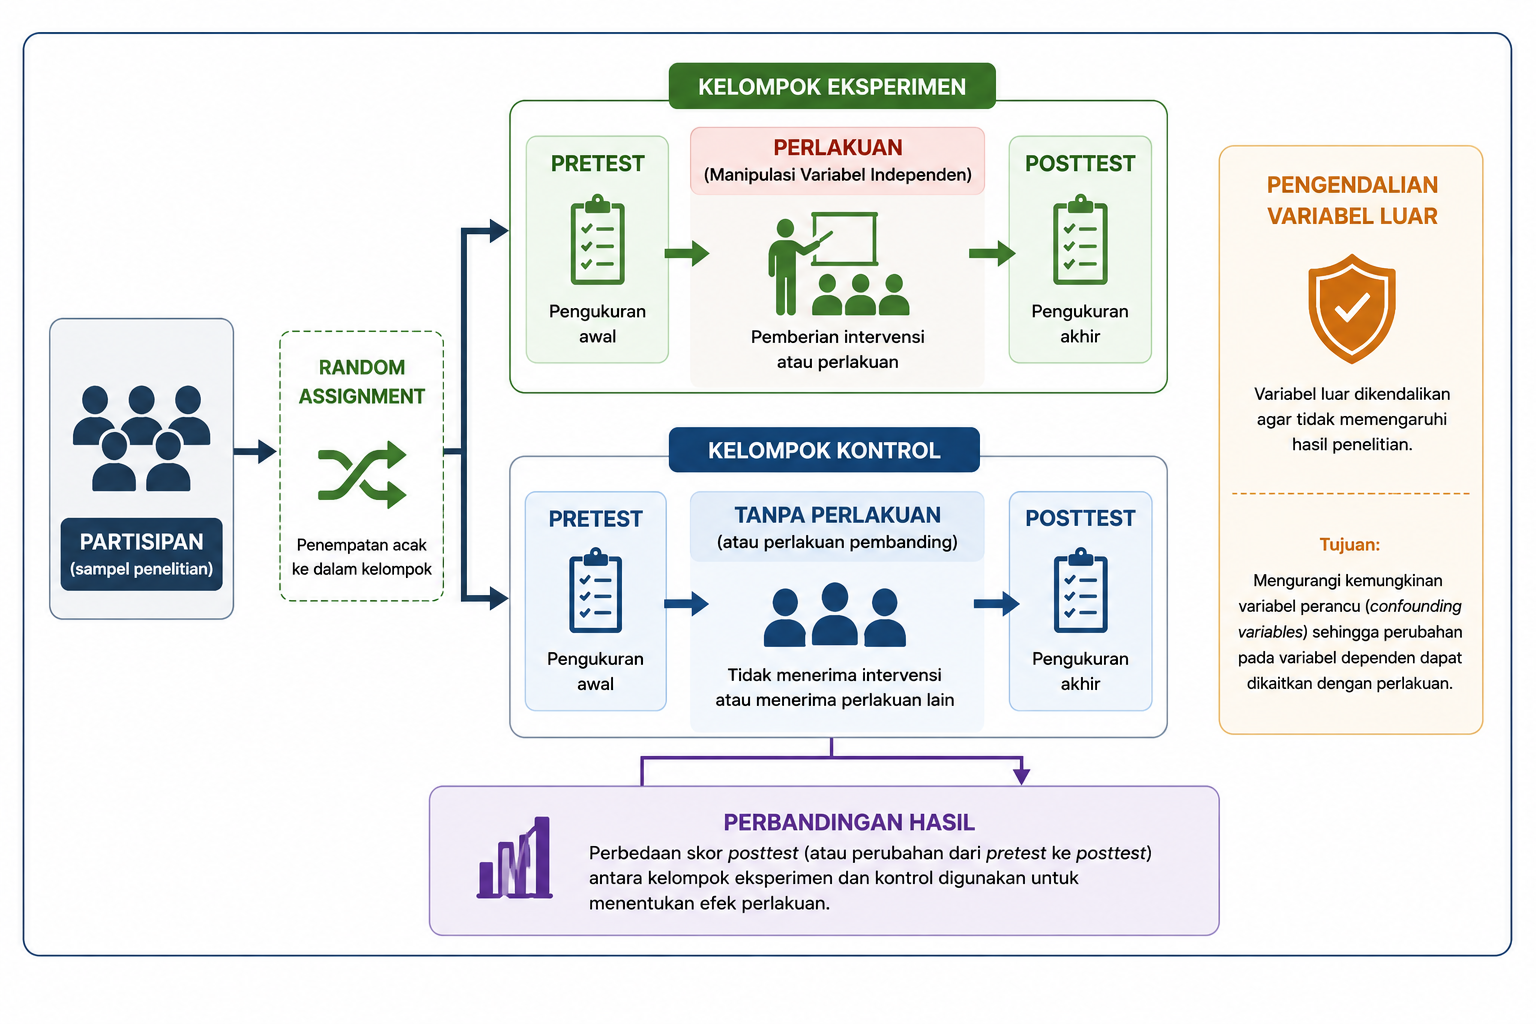
\includegraphics[keepaspectratio]{images/eksperimen_ch13.png}}
\caption{Unsur-unsur Pokok Penelitian Eksperimen}
\end{figure}

}

\caption{\label{fig-unsureksp}}

\end{figure}%

Sebagaimana ditunjukkan pada Gambar~\ref{fig-unsureksp}, kelima unsur
tersebut saling berkaitan dalam menghasilkan penelitian eksperimen yang
memiliki validitas internal yang tinggi. Semakin baik manipulasi
dilakukan, semakin efektif pengendalian variabel luar, semakin seimbang
karakteristik kelompok melalui r\emph{andom assignment}, serta semakin
tepat pengukuran hasil dilakukan, maka semakin kuat pula dasar peneliti
dalam menyimpulkan bahwa perubahan pada variabel dependen berkaitan
dengan perlakuan yang diberikan.

Pada subbab berikutnya akan dibahas bagaimana kelima unsur tersebut
diterapkan dalam berbagai jenis desain eksperimen, mulai dari
pra-eksperimen, kuasi eksperimen, hingga eksperimen murni.

\section{Klasifikasi Desain
Eksperimen}\label{klasifikasi-desain-eksperimen}

Penelitian eksperimen tidak selalu dilaksanakan dengan tingkat
pengendalian yang sama. Dalam praktiknya, keterbatasan etika, kondisi
lapangan, maupun karakteristik partisipan sering kali memengaruhi sejauh
mana peneliti dapat menerapkan manipulasi, kelompok pembanding/kontrol,
dan \emph{random assignment}. Oleh karena itu, desain eksperimen
diklasifikasikan berdasarkan tingkat kontrol yang dimiliki peneliti
terhadap jalannya penelitian.

Secara umum, desain eksperimen dibedakan menjadi tiga kelompok, yaitu
pra-eksperimen (\emph{pre-experiment}), kuasi eksperimen
(\emph{quasi-experiment}), dan eksperimen murni (\emph{true experiment}
atau \emph{randomized experiment}) (Campbell \& Stanley, 1963; Creswell
\& Creswell, 2023; Shadish dkk., 2002). Perbedaan utama ketiga desain
tersebut terletak pada ada atau tidaknya kelompok pembanding,
\emph{random assignment}, serta kemampuan peneliti mengendalikan
variabel luar. Semakin tinggi tingkat kontrol yang diterapkan, semakin
kuat pula validitas internal dan inferensi kausal yang dapat dihasilkan.

Namun demikian, bukan berarti eksperimen murni selalu menjadi pilihan
terbaik. Pemilihan desain tetap harus disesuaikan dengan tujuan
penelitian, kondisi lapangan, serta pertimbangan etis dalam pelaksanaan
penelitian. Tabel~\ref{tbl-desaineksp} memberikan gambaran umum mengenai
karakteristik masing-masing jenis desain eksperimen.

\begin{longtable}[]{@{}
  >{\raggedright\arraybackslash}p{(\linewidth - 6\tabcolsep) * \real{0.2500}}
  >{\centering\arraybackslash}p{(\linewidth - 6\tabcolsep) * \real{0.2500}}
  >{\centering\arraybackslash}p{(\linewidth - 6\tabcolsep) * \real{0.2500}}
  >{\centering\arraybackslash}p{(\linewidth - 6\tabcolsep) * \real{0.2500}}@{}}
\caption{Perbandingan Umum Desain
Eksperimen}\label{tbl-desaineksp}\tabularnewline
\toprule\noalign{}
\endfirsthead
\endhead
\bottomrule\noalign{}
\endlastfoot
\textbf{Karakteristik} & \textbf{Pra-eksperimen} & \textbf{Kuasi
eksperimen} & \textbf{Eksperimen murni} \\
Manipulasi variabel independen & ✓ & ✓ & ✓ \\
Kelompok pembanding & Tidak selalu ada & Ada & Ada \\
\emph{Random assignment} & ✗ & ✗ & ✓ \\
Kontrol terhadap variabel luar & Rendah & Sedang & Tinggi \\
Validitas internal & Rendah & Sedang & Tinggi \\
Kekuatan inferensi kausal & Rendah & Sedang & Tinggi \\
\end{longtable}

\subsection{Pra-Eksperimen}\label{pra-eksperimen}

Pra-eksperimen merupakan bentuk eksperimen dengan tingkat kontrol yang
paling rendah. Penelitian ini tetap melibatkan pemberian perlakuan,
tetapi umumnya tidak menggunakan random assignment dan sering kali tidak
memiliki kelompok pembanding yang memadai. Akibatnya, perubahan yang
terjadi setelah perlakuan belum dapat dipastikan sepenuhnya sebagai
akibat dari perlakuan tersebut karena masih terdapat kemungkinan
dipengaruhi oleh faktor lain. Meskipun demikian, pra-eksperimen tetap
bermanfaat sebagai studi pendahuluan, uji coba intervensi, atau evaluasi
awal sebelum dilakukan penelitian dengan desain yang lebih kuat
(Campbell \& Stanley, 1963; Gravetter \& Forzano, 2018).

\textbf{Kelebihan dan keterbatasan.} Kelebihan utama pra-eksperimen
adalah prosedurnya relatif sederhana, mudah dilaksanakan, serta
membutuhkan sumber daya yang lebih sedikit dibandingkan desain
eksperimen lainnya. Oleh karena itu, desain ini sering digunakan sebagai
studi pendahuluan (\emph{pilot study}), evaluasi awal suatu program,
atau uji coba intervensi sebelum dilakukan penelitian yang lebih
komprehensif. Namun, karena umumnya tidak menggunakan kelompok
pembanding maupun random assignment, validitas internalnya relatif
rendah. Akibatnya, perubahan yang diamati setelah perlakuan belum dapat
dipastikan sepenuhnya disebabkan oleh perlakuan, sehingga hasil
penelitian perlu diinterpretasikan secara hati-hati (Campbell \&
Stanley, 1963; Gravetter \& Forzano, 2018).

\subsection{Kuasi Eksperimen}\label{kuasi-eksperimen}

Kuasi eksperimen merupakan alternatif ketika peneliti tidak memungkinkan
melakukan random assignment, tetapi masih dapat memberikan perlakuan dan
menggunakan kelompok pembanding. Kelompok penelitian biasanya telah
terbentuk secara alami, misalnya berdasarkan kelas, sekolah, unit kerja,
atau komunitas. Dibandingkan pra-eksperimen, kuasi eksperimen memiliki
validitas internal yang lebih baik karena adanya kelompok pembanding,
meskipun inferensi kausal yang dihasilkan masih lebih lemah dibandingkan
eksperimen murni (Morling, 2024; Shadish dkk., 2002).

\textbf{Kelebihan dan keterbatasan.} Kuasi eksperimen memiliki kelebihan
berupa fleksibilitas yang lebih tinggi sehingga dapat diterapkan pada
situasi nyata ketika random assignment tidak memungkinkan dilakukan,
misalnya pada penelitian di sekolah, rumah sakit, organisasi, atau
komunitas. Desain ini tetap memungkinkan peneliti mengevaluasi
efektivitas suatu program atau intervensi dalam kondisi lapangan.
Meskipun demikian, tidak adanya random assignment menyebabkan
kemungkinan adanya perbedaan karakteristik awal antar kelompok yang
dapat memengaruhi hasil penelitian. Oleh karena itu, inferensi kausal
yang dihasilkan lebih terbatas dibandingkan eksperimen murni, sehingga
peneliti perlu menerapkan prosedur pengendalian yang memadai untuk
meningkatkan validitas internal (Morling, 2024; Shadish dkk., 2002).

\subsection{Eksperimen Murni}\label{eksperimen-murni}

Eksperimen murni (\emph{true experiment}) merupakan desain eksperimen
dengan tingkat kontrol tertinggi. Desain ini mengombinasikan manipulasi
variabel independen, kelompok pembanding, serta random assignment
sehingga peneliti memiliki dasar yang lebih kuat untuk menyimpulkan
hubungan sebab-akibat. Karena mampu meminimalkan pengaruh variabel
perancu, eksperimen murni sering dianggap sebagai standar terbaik
(\emph{gold standard}) dalam penelitian intervensi dan evaluasi
efektivitas suatu program. Namun, penerapannya sering menghadapi kendala
praktis maupun etis sehingga tidak selalu dapat digunakan dalam setiap
penelitian (Campbell \& Stanley, 1963; Creswell \& Creswell, 2023).

\textbf{Kelebihan dan keterbatasan.} Eksperimen murni memiliki
keunggulan utama dalam menghasilkan bukti yang paling kuat mengenai
hubungan sebab-akibat karena mengombinasikan manipulasi, kelompok
kontrol, dan random assignment. Tingginya tingkat kontrol terhadap
variabel luar menjadikan desain ini memiliki validitas internal yang
lebih baik dibandingkan desain eksperimen lainnya. Namun, penerapan
eksperimen murni sering kali menghadapi berbagai kendala praktis dan
etis, seperti kesulitan melakukan \emph{random assignment}, kebutuhan
sumber daya yang lebih besar, serta keterbatasan dalam menerapkan
intervensi pada situasi nyata. Oleh karena itu, meskipun sering dianggap
sebagai \emph{gold standard} dalam penelitian eksperimen, desain ini
tidak selalu menjadi pilihan yang paling sesuai untuk setiap konteks
penelitian (Campbell \& Stanley, 1963; Creswell \& Creswell, 2023).

Berdasarkan uraian tersebut, dapat dipahami bahwa ketiga desain
eksperimen memiliki fungsi dan karakteristik yang berbeda.
Pra-eksperimen lebih sesuai digunakan untuk studi awal dengan kontrol
yang terbatas, kuasi eksperimen menjadi pilihan ketika random assignment
tidak memungkinkan, sedangkan eksperimen murni digunakan apabila
peneliti dapat menerapkan kontrol yang optimal terhadap jalannya
penelitian.

\section{Struktur Kondisi dalam Penelitian
Eksperimen}\label{struktur-kondisi-dalam-penelitian-eksperimen}

Selain dibedakan berdasarkan tingkat kontrolnya, penelitian eksperimen
juga dapat dibedakan berdasarkan cara partisipan mengikuti kondisi
eksperimen. Perbedaan ini dikenal sebagai \textbf{struktur kondisi}
(\emph{experimental design structure}), yaitu bagaimana perlakuan
diberikan kepada partisipan dan bagaimana data dikumpulkan pada setiap
kondisi penelitian. Secara umum, terdapat dua struktur kondisi yang
paling sering digunakan, yaitu \textbf{\emph{between-subjects design}}
dan \textbf{\emph{within-subjects design}} (Gravetter \& Forzano, 2018;
Jhangiani dkk., 2019).

\subsection{\texorpdfstring{\emph{Between-subjects
Design}}{Between-subjects Design}}\label{between-subjects-design}

Pada \emph{between-subjects design}, setiap partisipan hanya mengikuti
satu kondisi eksperimen. Misalnya, sebagian peserta ditempatkan pada
kelompok eksperimen yang menerima pelatihan \emph{mindfulness},
sedangkan peserta lainnya berada pada kelompok kontrol yang tidak
menerima pelatihan. Dengan demikian, setiap peserta hanya memberikan
data untuk satu kondisi penelitian.

Kelebihan utama desain ini adalah tidak adanya pengaruh pengalaman dari
kondisi sebelumnya (\emph{carry-over effect}) karena setiap peserta
hanya mengikuti satu perlakuan. Namun, desain ini umumnya memerlukan
jumlah partisipan yang lebih banyak dan membutuhkan random assignment
atau prosedur lain agar karakteristik awal setiap kelompok relatif
seimbang.

\begin{figure}[H]

{\centering \pandocbounded{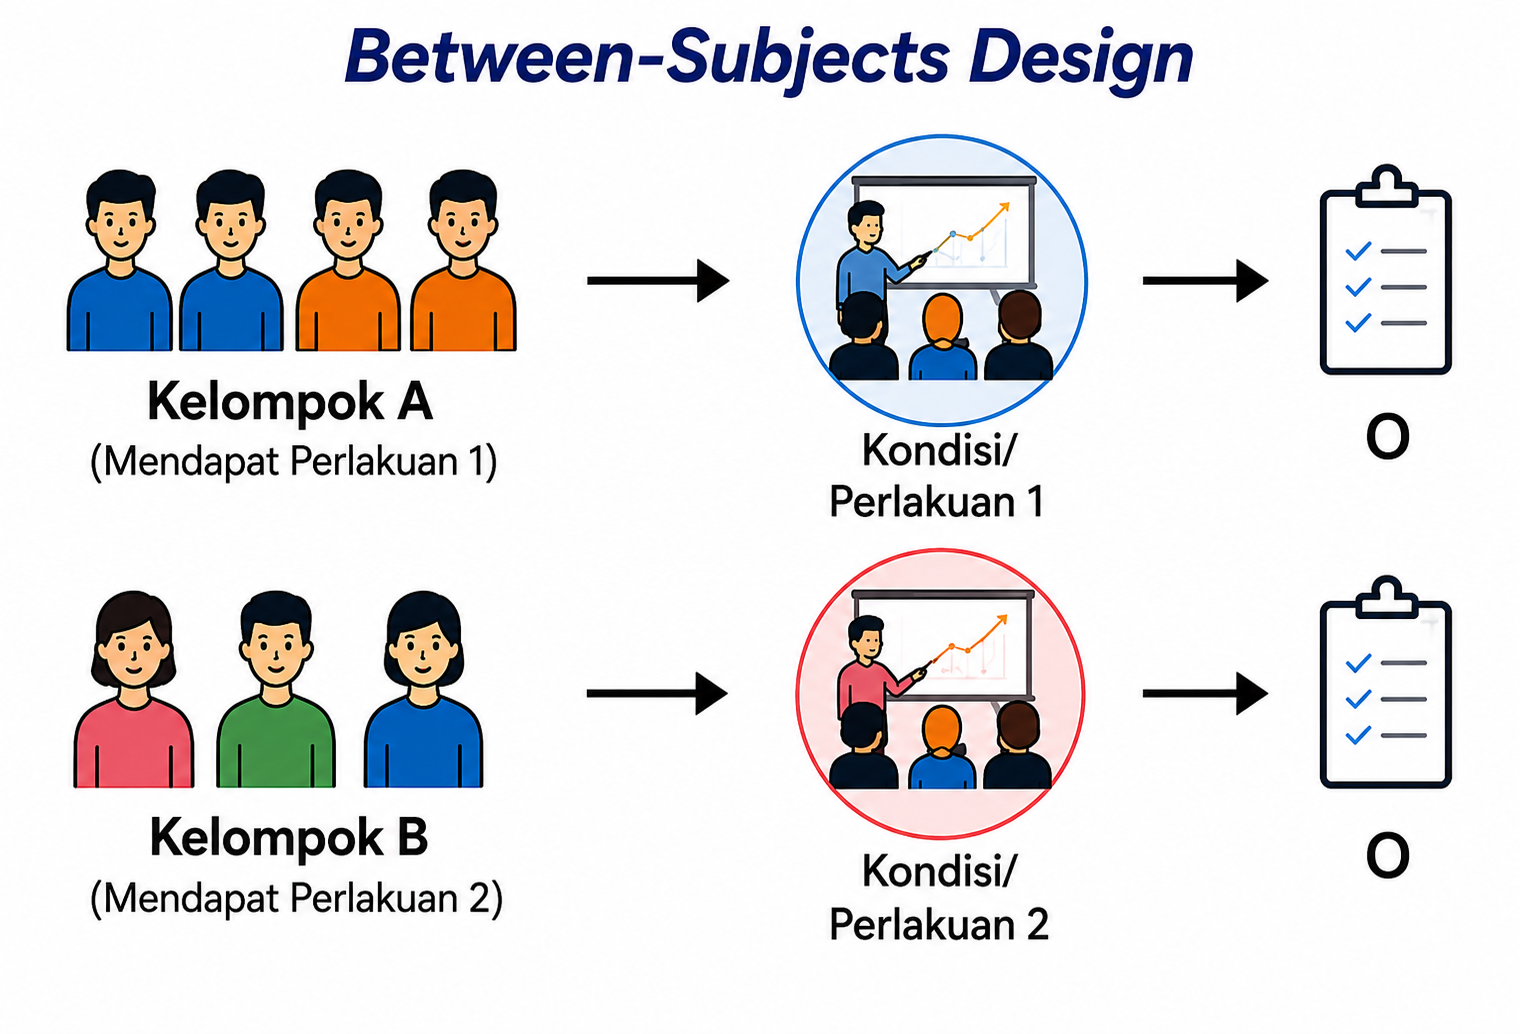
\includegraphics[keepaspectratio]{images/between2.png}}

}

\caption{Ilustrasi desain between-subjects}

\end{figure}%

\subsection{\texorpdfstring{\emph{Within-subjecst
Design}}{Within-subjecst Design}}\label{within-subjecst-design}

Pada \emph{within-subjects design}, setiap partisipan mengikuti seluruh
kondisi eksperimen. Sebagai contoh, seorang peserta diminta mengikuti
beberapa jenis strategi regulasi emosi, seperti latihan pernapasan
sadar, menulis reflektif, dan kondisi tanpa perlakuan. Setelah setiap
kondisi selesai, peneliti mengukur tingkat stres atau variabel lain yang
menjadi fokus penelitian.

Keunggulan desain ini adalah membutuhkan jumlah partisipan yang lebih
sedikit dan mampu mengurangi pengaruh perbedaan individual karena setiap
peserta menjadi pembanding bagi dirinya sendiri. Namun, desain ini
memiliki kelemahan berupa kemungkinan munculnya \textbf{\emph{carry-over
effect}}, yaitu pengaruh dari kondisi sebelumnya terhadap kondisi
berikutnya. Untuk meminimalkan hal tersebut, peneliti dapat mengatur
urutan pemberian perlakuan menggunakan teknik
\textbf{\emph{counterbalancing}}.

\begin{figure}[H]

{\centering \pandocbounded{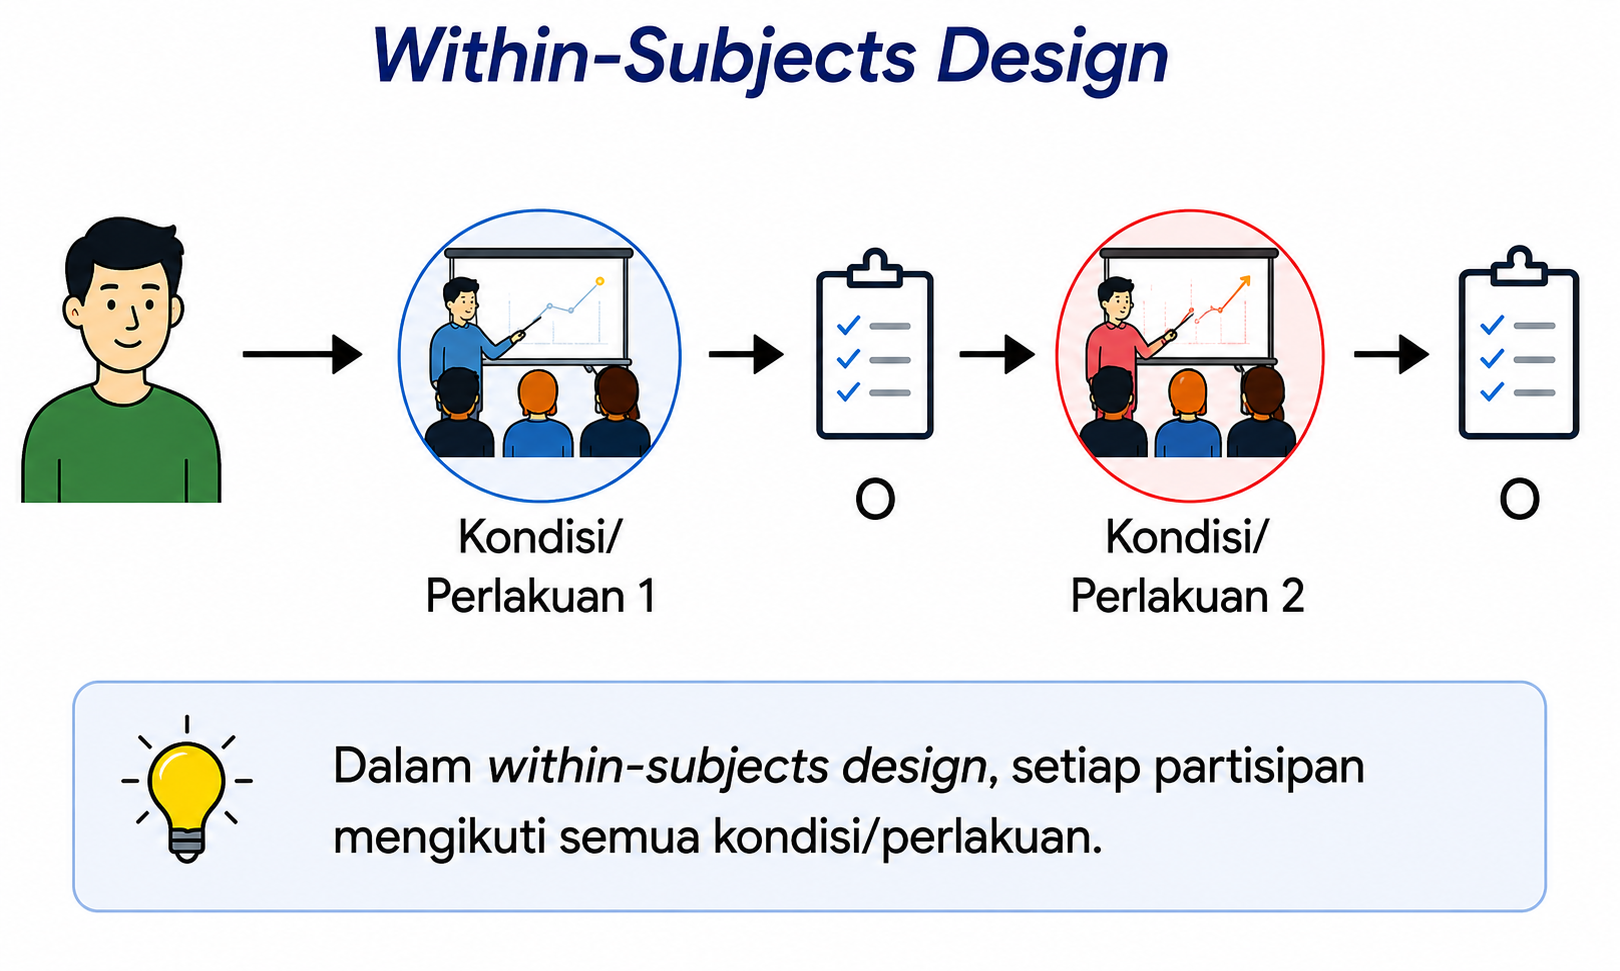
\includegraphics[keepaspectratio]{images/within2.png}}

}

\caption{Ilustrasi desain within-subjects}

\end{figure}%

\subsection{\texorpdfstring{\emph{Perbandingan Between-subjects dan
Within-subjects
Design}}{Perbandingan Between-subjects dan Within-subjects Design}}\label{perbandingan-between-subjects-dan-within-subjects-design}

Pemilihan struktur kondisi bergantung pada tujuan penelitian,
karakteristik perlakuan, serta kemungkinan munculnya efek urutan.
\emph{Between-subjects design} lebih sesuai apabila perlakuan memiliki
efek yang menetap atau sulit dihilangkan, misalnya program pelatihan,
terapi psikologis, atau intervensi pendidikan. Sebaliknya,
\emph{within-subjects design} lebih tepat digunakan apabila setiap
peserta dapat mengikuti seluruh kondisi penelitian tanpa menimbulkan
efek bawaan yang berarti. Kedua struktur tersebut dapat diterapkan pada
berbagai bentuk eksperimen, baik pra-eksperimen, kuasi eksperimen,
maupun eksperimen murni, sesuai dengan tujuan dan karakteristik
penelitian.

Tabel 13.2 merangkum perbedaan utama kedua struktur kondisi tersebut.

\begin{longtable}[]{@{}
  >{\raggedright\arraybackslash}p{(\linewidth - 4\tabcolsep) * \real{0.3333}}
  >{\raggedright\arraybackslash}p{(\linewidth - 4\tabcolsep) * \real{0.3333}}
  >{\raggedright\arraybackslash}p{(\linewidth - 4\tabcolsep) * \real{0.3333}}@{}}
\caption{Perbandingan \emph{Between-subjects Design} dan
\emph{Within-subjects Design}}\label{tbl-struktur}\tabularnewline
\toprule\noalign{}
\endfirsthead
\endhead
\bottomrule\noalign{}
\endlastfoot
\textbf{Aspek} & \textbf{\emph{Between-subjects design}} &
\textbf{\emph{Within-subjects design}} \\
Partisipan & Setiap peserta hanya mengikuti satu kondisi & Setiap
peserta mengikuti seluruh kondisi \\
Jumlah partisipan & Relatif lebih banyak & Relatif lebih sedikit \\
Pengaruh perbedaan individual & Lebih besar & Lebih kecil \\
\emph{Carry-over effect} & Tidak ada & Berpotensi terjadi \\
\emph{Counterbalancing} & Umumnya tidak diperlukan & Umumnya
diperlukan \\
Contoh penggunaan & Membandingkan kelompok eksperimen dan kelompok
kontrol & Membandingkan beberapa perlakuan pada peserta yang sama \\
\end{longtable}

Secara umum, kedua struktur kondisi tersebut memiliki kelebihan dan
keterbatasan masing-masing. Oleh karena itu, peneliti perlu memilih
struktur yang paling sesuai dengan tujuan penelitian, jenis perlakuan
yang diberikan, serta kondisi pelaksanaan penelitian. Pemahaman mengenai
kedua struktur ini juga akan membantu peneliti dalam memilih bentuk
desain eksperimen yang akan dibahas pada bagian berikutnya.

\section{Bentuk-bentuk Desain
Eksperimen}\label{bentuk-bentuk-desain-eksperimen}

Setelah memahami klasifikasi desain eksperimen, peneliti perlu mengenal
berbagai bentuk rancangan yang umum digunakan dalam praktik penelitian.
Masing-masing bentuk desain memiliki karakteristik yang berbeda,
terutama dalam hal penggunaan kelompok pembanding, pengukuran sebelum
dan sesudah perlakuan, serta cara penempatan partisipan ke dalam
kelompok penelitian. Pemilihan bentuk desain perlu disesuaikan dengan
tujuan penelitian, kondisi lapangan, serta tingkat kontrol yang dapat
diterapkan oleh peneliti (Campbell \& Stanley, 1963; Shadish dkk.,
2002).

\subsection{Bentuk-bentuk
Pra-Eksperimen}\label{bentuk-bentuk-pra-eksperimen}

Pra-eksperimen memiliki beberapa bentuk rancangan yang sederhana dan
umumnya digunakan ketika peneliti belum dapat menerapkan kelompok
kontrol maupun \emph{random assignment}.

\subsubsection{\texorpdfstring{\emph{One-shot case
study}}{One-shot case study}}\label{one-shot-case-study}

Pada desain ini, satu kelompok diberikan perlakuan, kemudian dilakukan
pengukuran setelah perlakuan selesai. Desain ini merupakan bentuk
pra-eksperimen yang paling sederhana karena tidak menggunakan pretest
maupun kelompok pembanding.

\begin{figure}[H]

{\centering \pandocbounded{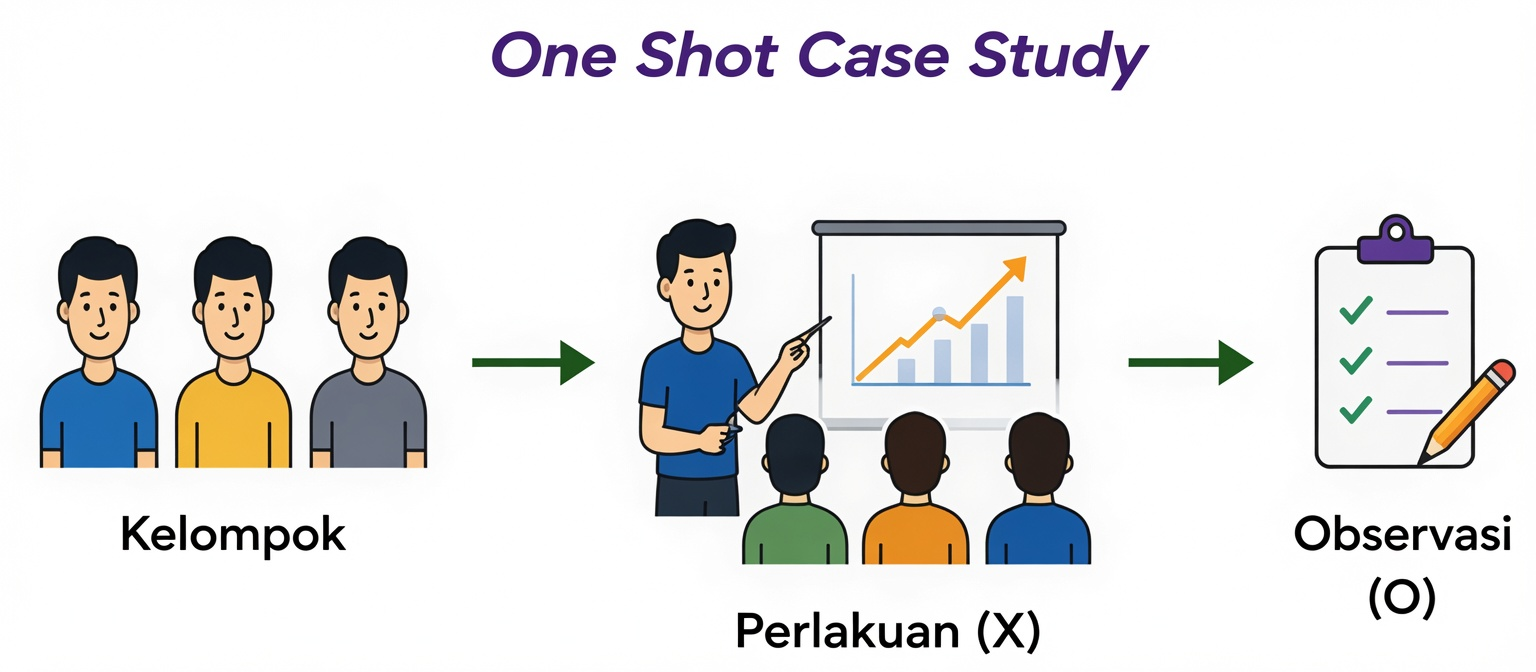
\includegraphics[keepaspectratio]{images/one.jpg}}

}

\caption{Ilustrasi desain one-shot case study}

\end{figure}%

\subsubsection{\texorpdfstring{\emph{One-group pretest-posttest
design}}{One-group pretest-posttest design}}\label{one-group-pretest-posttest-design}

Pada desain ini, satu kelompok diukur sebelum dan sesudah perlakuan.
Adanya \emph{pretest} memungkinkan peneliti membandingkan perubahan yang
terjadi sebelum dan sesudah perlakuan. Namun, karena tidak terdapat
kelompok pembanding, perubahan tersebut belum tentu sepenuhnya
disebabkan oleh perlakuan.

\begin{figure}[H]

{\centering \pandocbounded{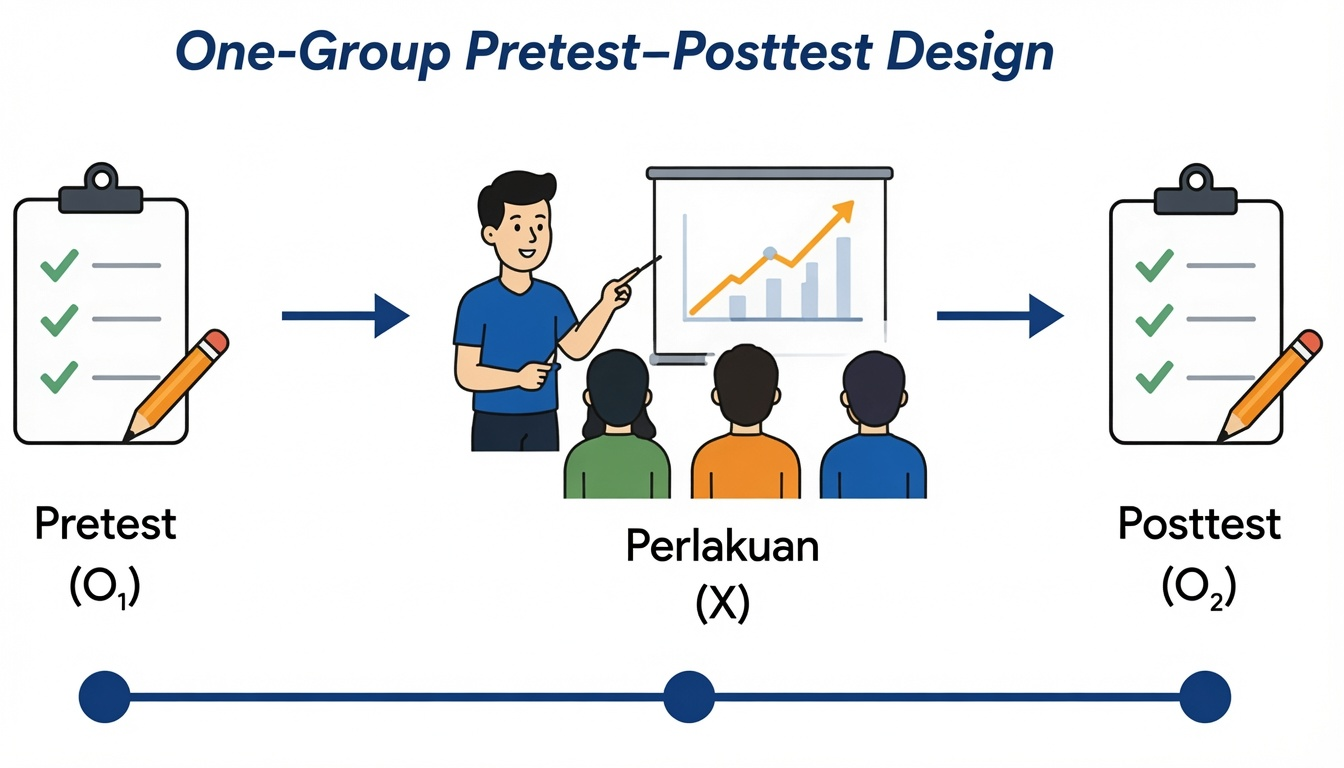
\includegraphics[keepaspectratio]{images/onegroupprepost.jpg}}

}

\caption{Ilustrasi desain one-group pretest-posttest}

\end{figure}%

\subsubsection{\texorpdfstring{\emph{Static-group
comparison}}{Static-group comparison}}\label{static-group-comparison}

Pada desain ini terdapat dua kelompok, tetapi peserta tidak ditempatkan
secara acak dan tidak dilakukan \emph{pretest}. Desain ini memungkinkan
adanya perbandingan hasil antar kelompok, tetapi masih memiliki
kelemahan karena karakteristik awal kedua kelompok mungkin sudah berbeda
sebelum penelitian dimulai.

\begin{figure}[H]

{\centering \pandocbounded{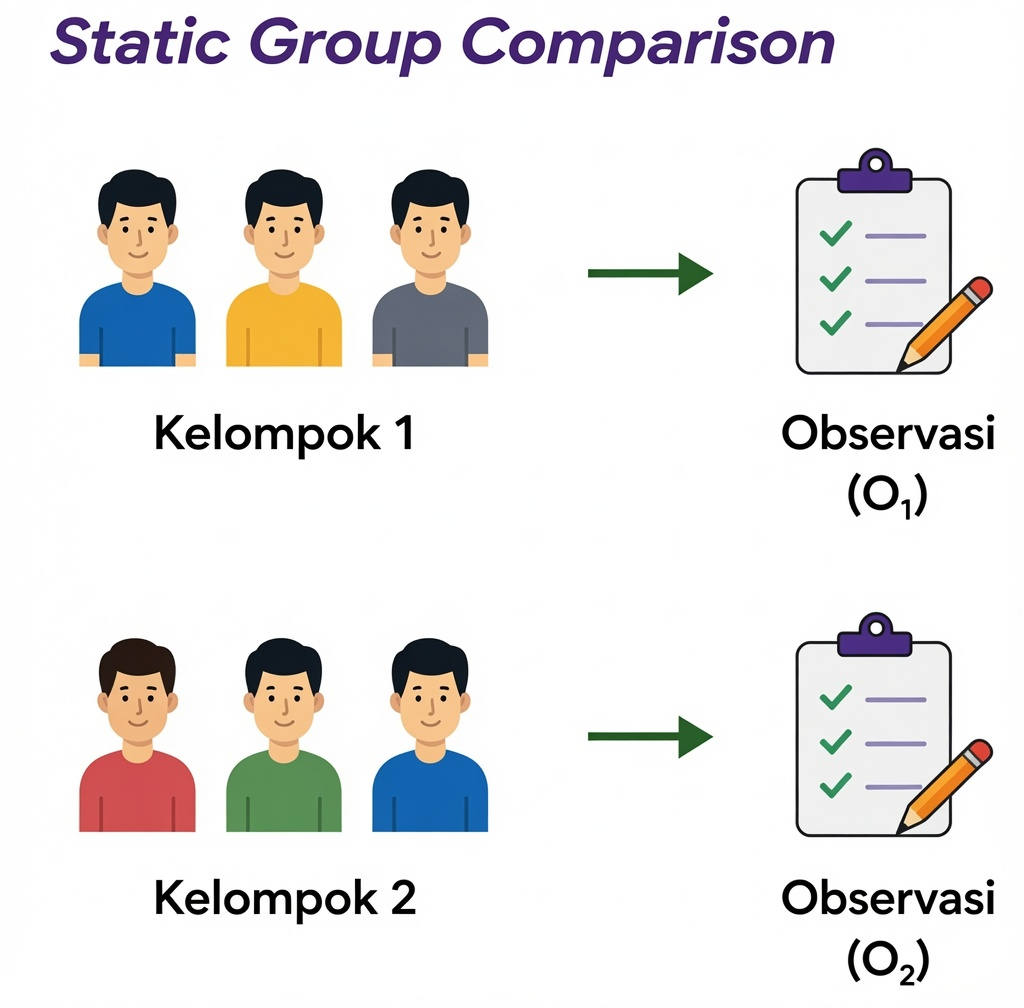
\includegraphics[keepaspectratio]{images/static2.jpg}}

}

\caption{Ilustrasi desain static-group comparison}

\end{figure}%

\subsection{Bentuk-bentuk Kuasi
Eksperimen}\label{bentuk-bentuk-kuasi-eksperimen}

Kuasi eksperimen digunakan ketika \emph{random assignment} tidak
memungkinkan dilakukan, tetapi peneliti masih dapat memberikan perlakuan
dan menggunakan kelompok pembanding.

\subsubsection{\texorpdfstring{\emph{Nonequivalent control group
design}}{Nonequivalent control group design}}\label{nonequivalent-control-group-design}

Desain ini merupakan bentuk kuasi eksperimen yang paling sering
digunakan. Peneliti menggunakan kelompok eksperimen dan kelompok
pembanding yang telah terbentuk sebelumnya tanpa \emph{random
assignment}. Perbandingan hasil dilakukan dengan mempertimbangkan
kondisi awal kedua kelompok melalui \emph{pretest}.

\begin{figure}[H]

{\centering \pandocbounded{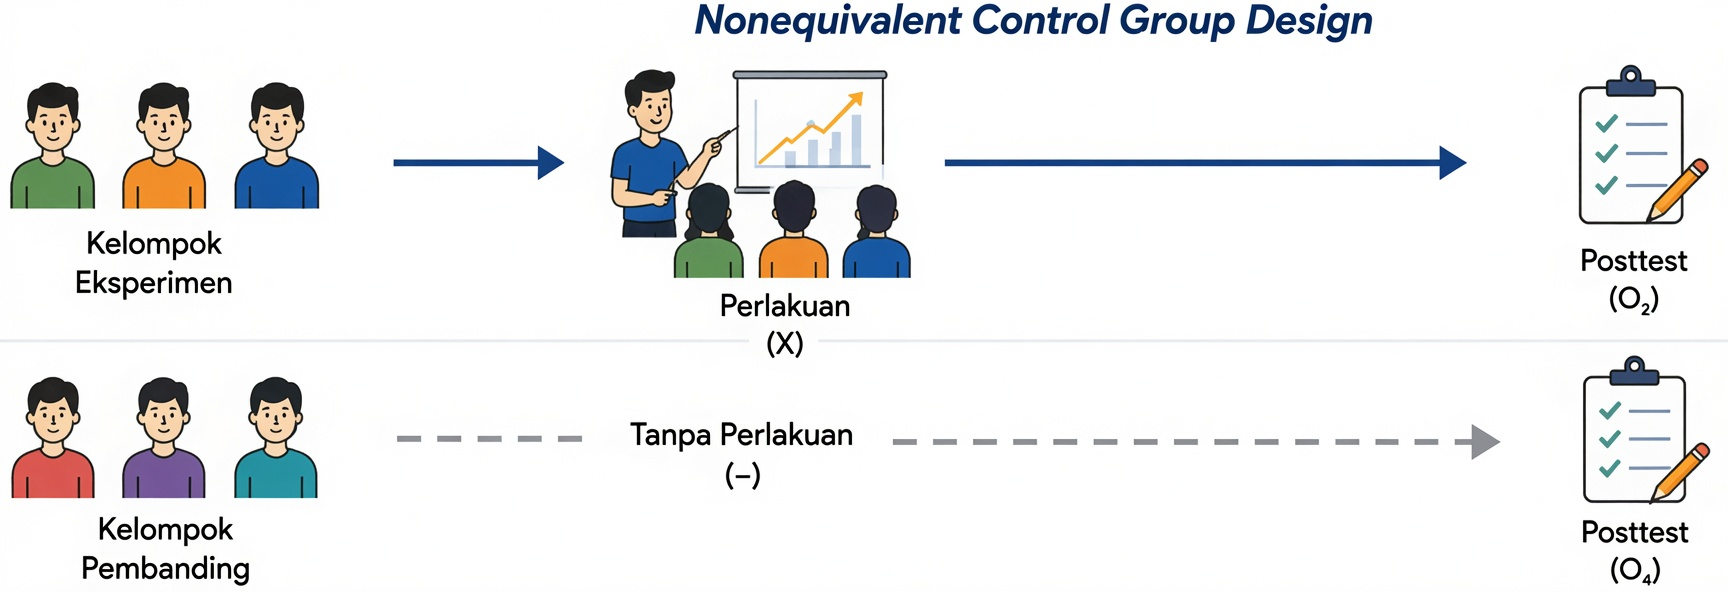
\includegraphics[keepaspectratio]{images/noneq.jpg}}

}

\caption{Ilustrasi desain nonequivalent control group}

\end{figure}%

\subsubsection{\texorpdfstring{\emph{Interrupted time-series
design}}{Interrupted time-series design}}\label{interrupted-time-series-design}

Pada desain ini, peneliti melakukan beberapa kali pengukuran sebelum dan
sesudah perlakuan sehingga perubahan dapat diamati sebagai suatu pola
dari waktu ke waktu. Desain ini bermanfaat ketika kelompok pembanding
sulit diperoleh, tetapi peneliti masih dapat melakukan pengukuran
berulang.

\begin{figure}[H]

{\centering \pandocbounded{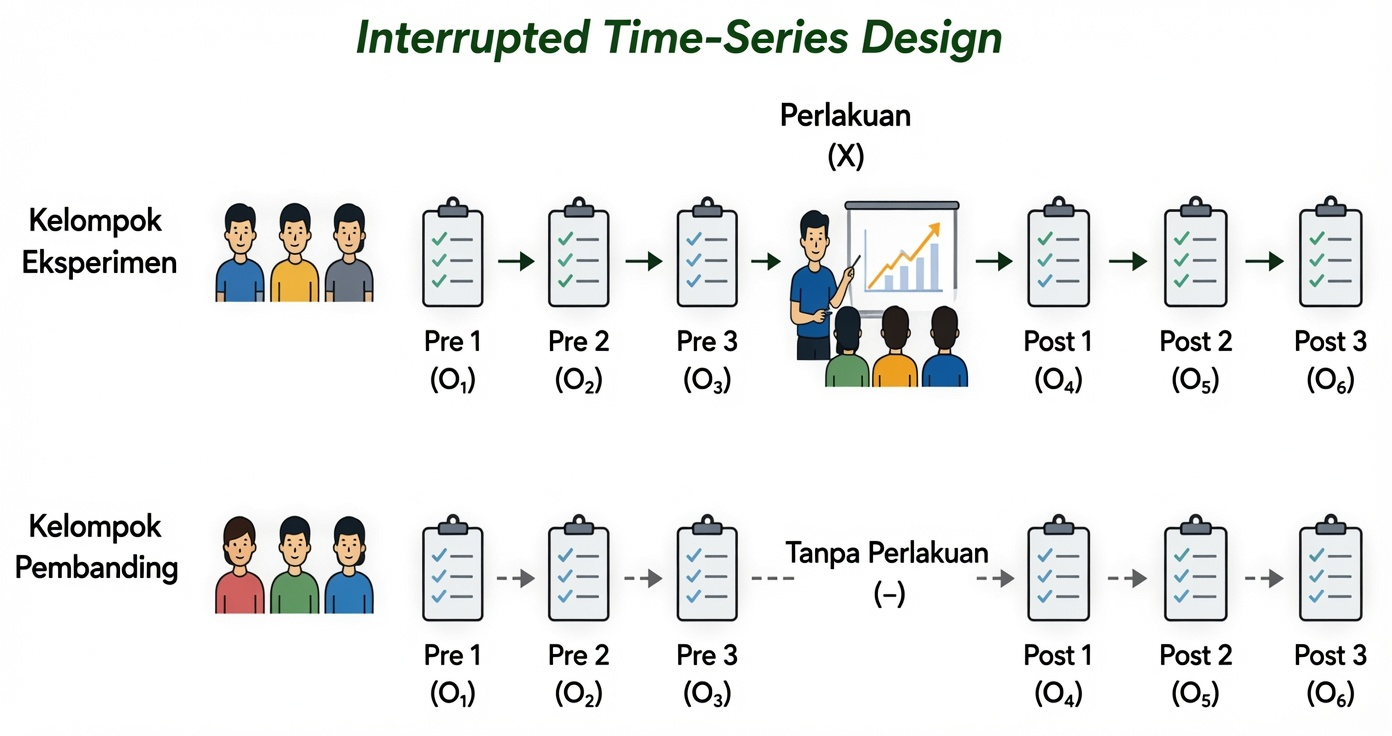
\includegraphics[keepaspectratio]{images/timeseries.jpg}}

}

\caption{Ilustrasi desain interrupted time-series}

\end{figure}%

\subsubsection{\texorpdfstring{\emph{Regression discontinuity
design}}{Regression discontinuity design}}\label{regression-discontinuity-design}

Desain ini digunakan ketika pemberian perlakuan didasarkan pada nilai
batas (\emph{cut-off score}). Contohnya, mahasiswa dengan tingkat stres
di atas skor tertentu memperoleh layanan konseling, sedangkan mahasiswa
dengan skor di bawah batas tersebut tidak memperoleh layanan yang sama.
Analisis kemudian dilakukan untuk mengetahui apakah terdapat perubahan
yang nyata di sekitar titik batas tersebut.

\begin{figure}[H]

{\centering \pandocbounded{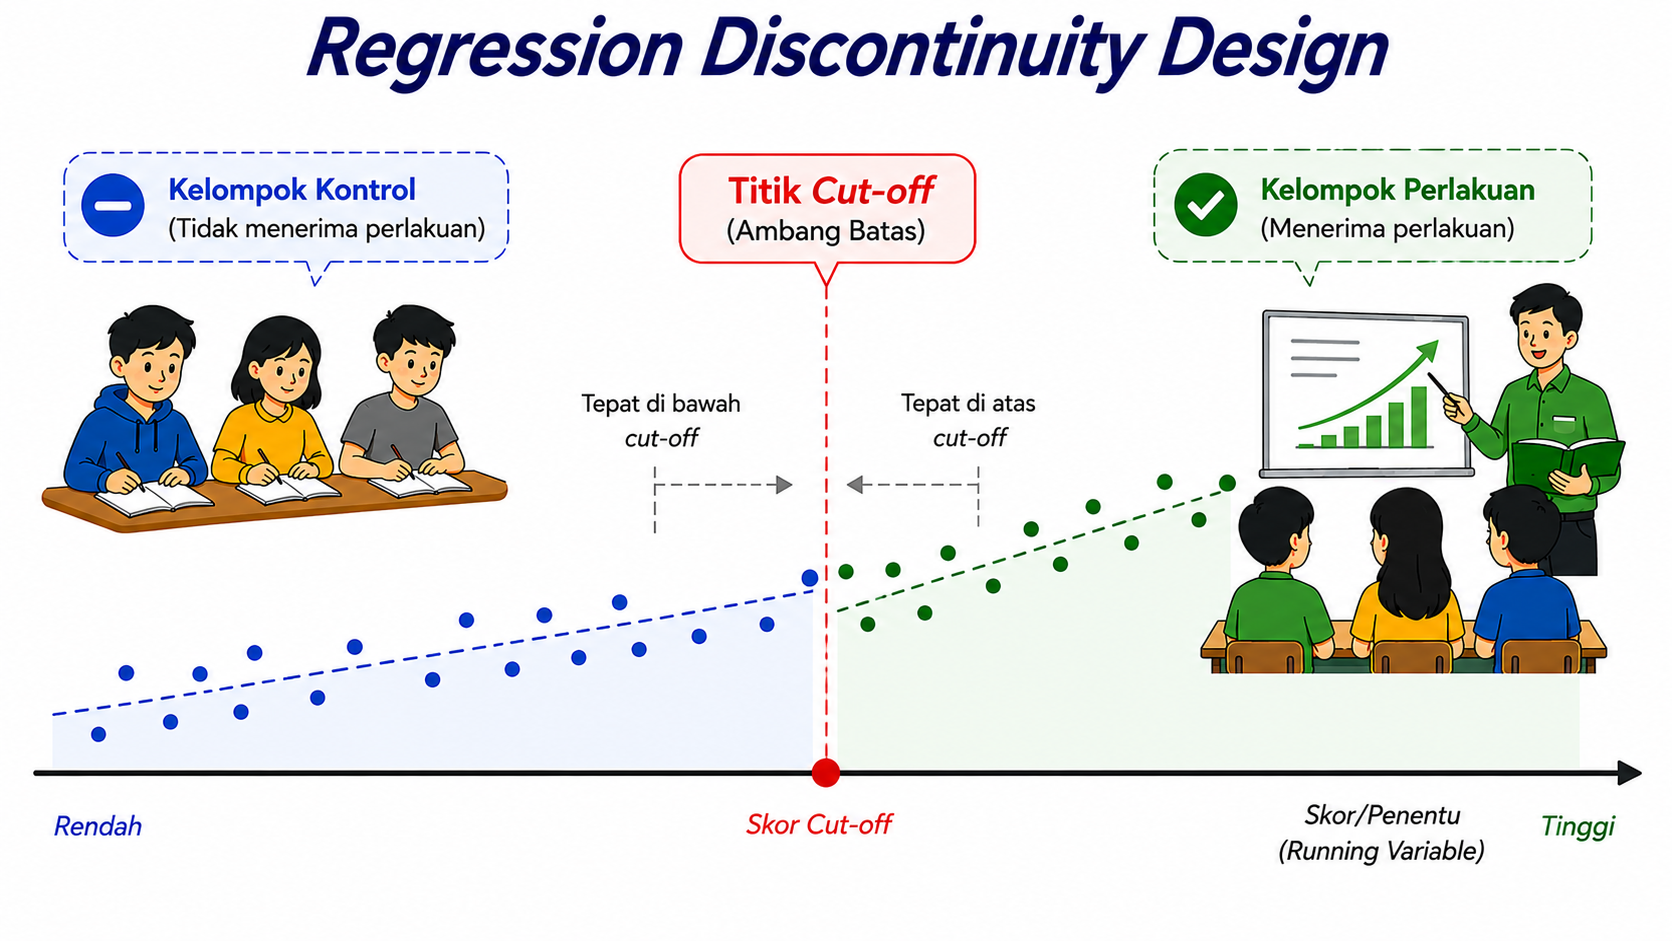
\includegraphics[keepaspectratio]{images/regres.png}}

}

\caption{Ilustrasi desain regression discontinuity}

\end{figure}%

\subsection{Bentuk-bentuk Eksperimen
Murni}\label{bentuk-bentuk-eksperimen-murni}

Eksperimen murni menggunakan manipulasi, kelompok pembanding, serta
\emph{random assignment} sehingga menghasilkan validitas internal yang
lebih tinggi dibandingkan bentuk desain lainnya.

\subsubsection{\texorpdfstring{\emph{Posttest-only control group
design}}{Posttest-only control group design}}\label{posttest-only-control-group-design}

Peserta dibagi secara acak ke dalam kelompok eksperimen dan kelompok
kontrol. Pengukuran hanya dilakukan setelah perlakuan diberikan. Desain
ini sesuai digunakan apabila \emph{pretest} diperkirakan dapat
memengaruhi respons peserta.

\begin{figure}[H]

{\centering \pandocbounded{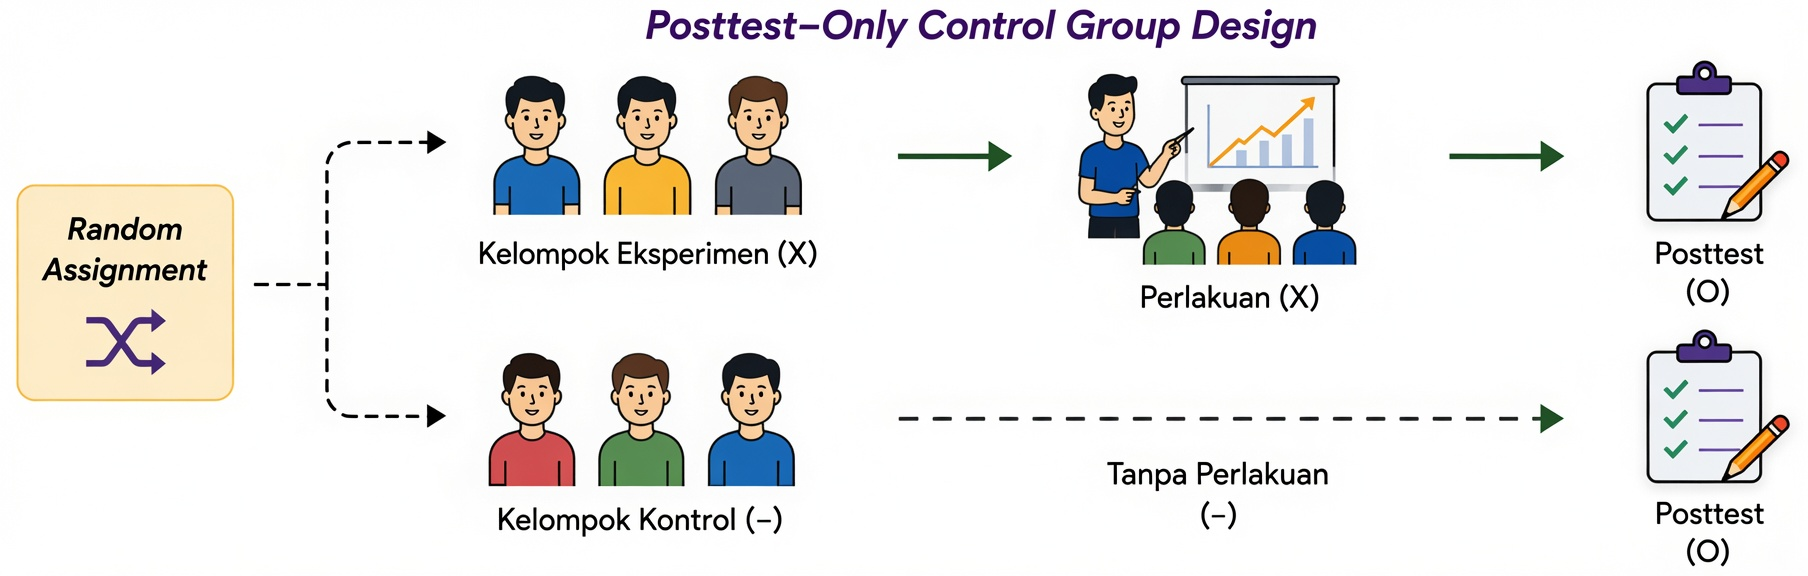
\includegraphics[keepaspectratio]{images/postonly2.png}}

}

\caption{Ilustrasi desain posttest-only control group}

\end{figure}%

\subsubsection{\texorpdfstring{\emph{Solomon four-group
design}}{Solomon four-group design}}\label{solomon-four-group-design}

Desain Solomon menggabungkan kelebihan desain \emph{posttest-only} dan
\emph{pretest-posttest} dengan menggunakan empat kelompok penelitian.
Dua kelompok diberikan \emph{pretest}, sedangkan dua kelompok lainnya
tidak. Desain ini digunakan untuk mengetahui apakah \emph{pretest} ikut
memengaruhi hasil penelitian (\emph{testing effect}), meskipun
membutuhkan jumlah partisipan yang lebih besar.

\begin{figure}[H]

{\centering \pandocbounded{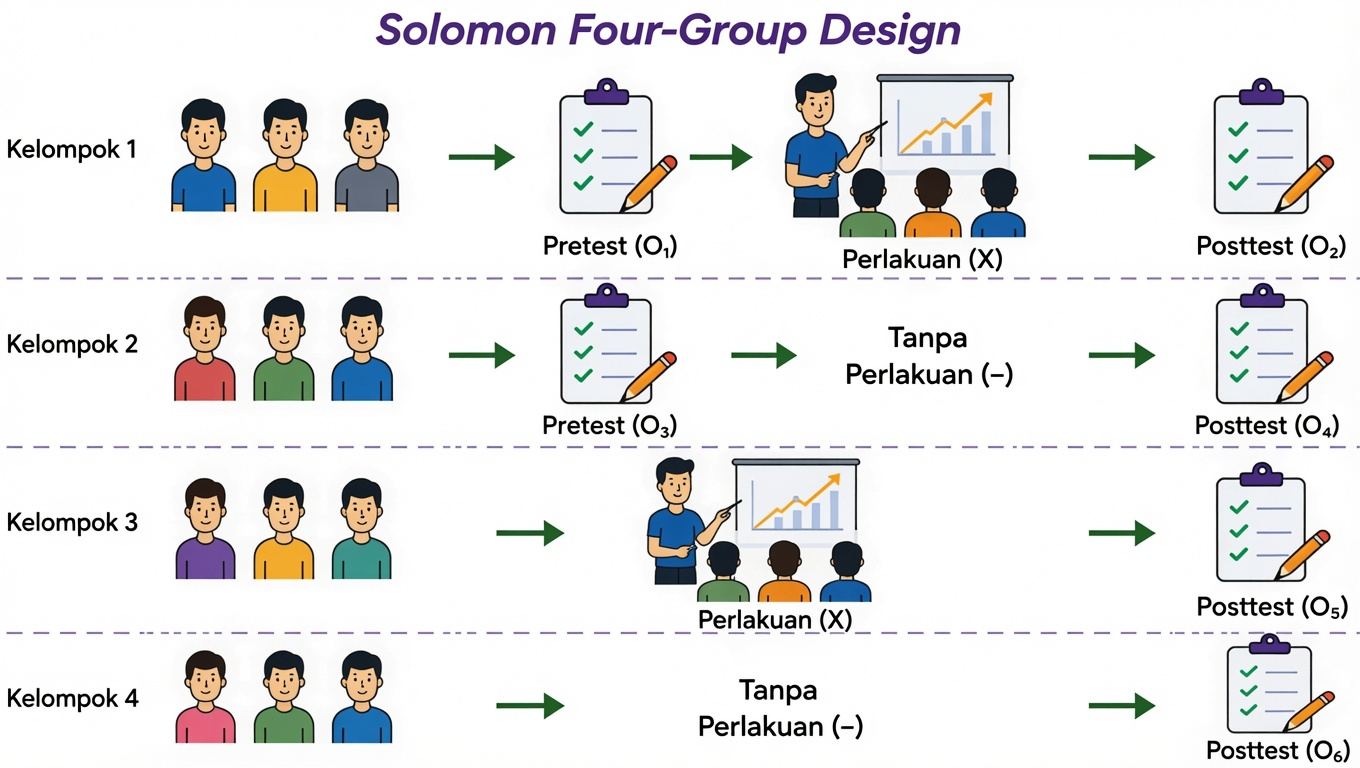
\includegraphics[keepaspectratio]{images/solomon.jpg}}

}

\caption{Ilustrasi desain Solomon four-group}

\end{figure}%

\subsubsection{\texorpdfstring{\emph{Factorial
design}}{Factorial design}}\label{factorial-design}

\emph{Factorial design} digunakan ketika penelitian melibatkan lebih
dari satu variabel independen. Selain menguji pengaruh masing-masing
variabel (\emph{main effect}), desain ini juga memungkinkan peneliti
menguji apakah terdapat interaksi (\emph{interaction effect})
antarvariabel independen. Sebagai contoh, peneliti dapat menguji
pengaruh \textbf{jenis pelatihan} (\emph{mindfulness} vs.~relaksasi) dan
\textbf{durasi pelatihan} (10 menit vs.~20 menit) terhadap stres
akademik mahasiswa menggunakan desain faktorial 2 × 2.

\begin{figure}[H]

{\centering \pandocbounded{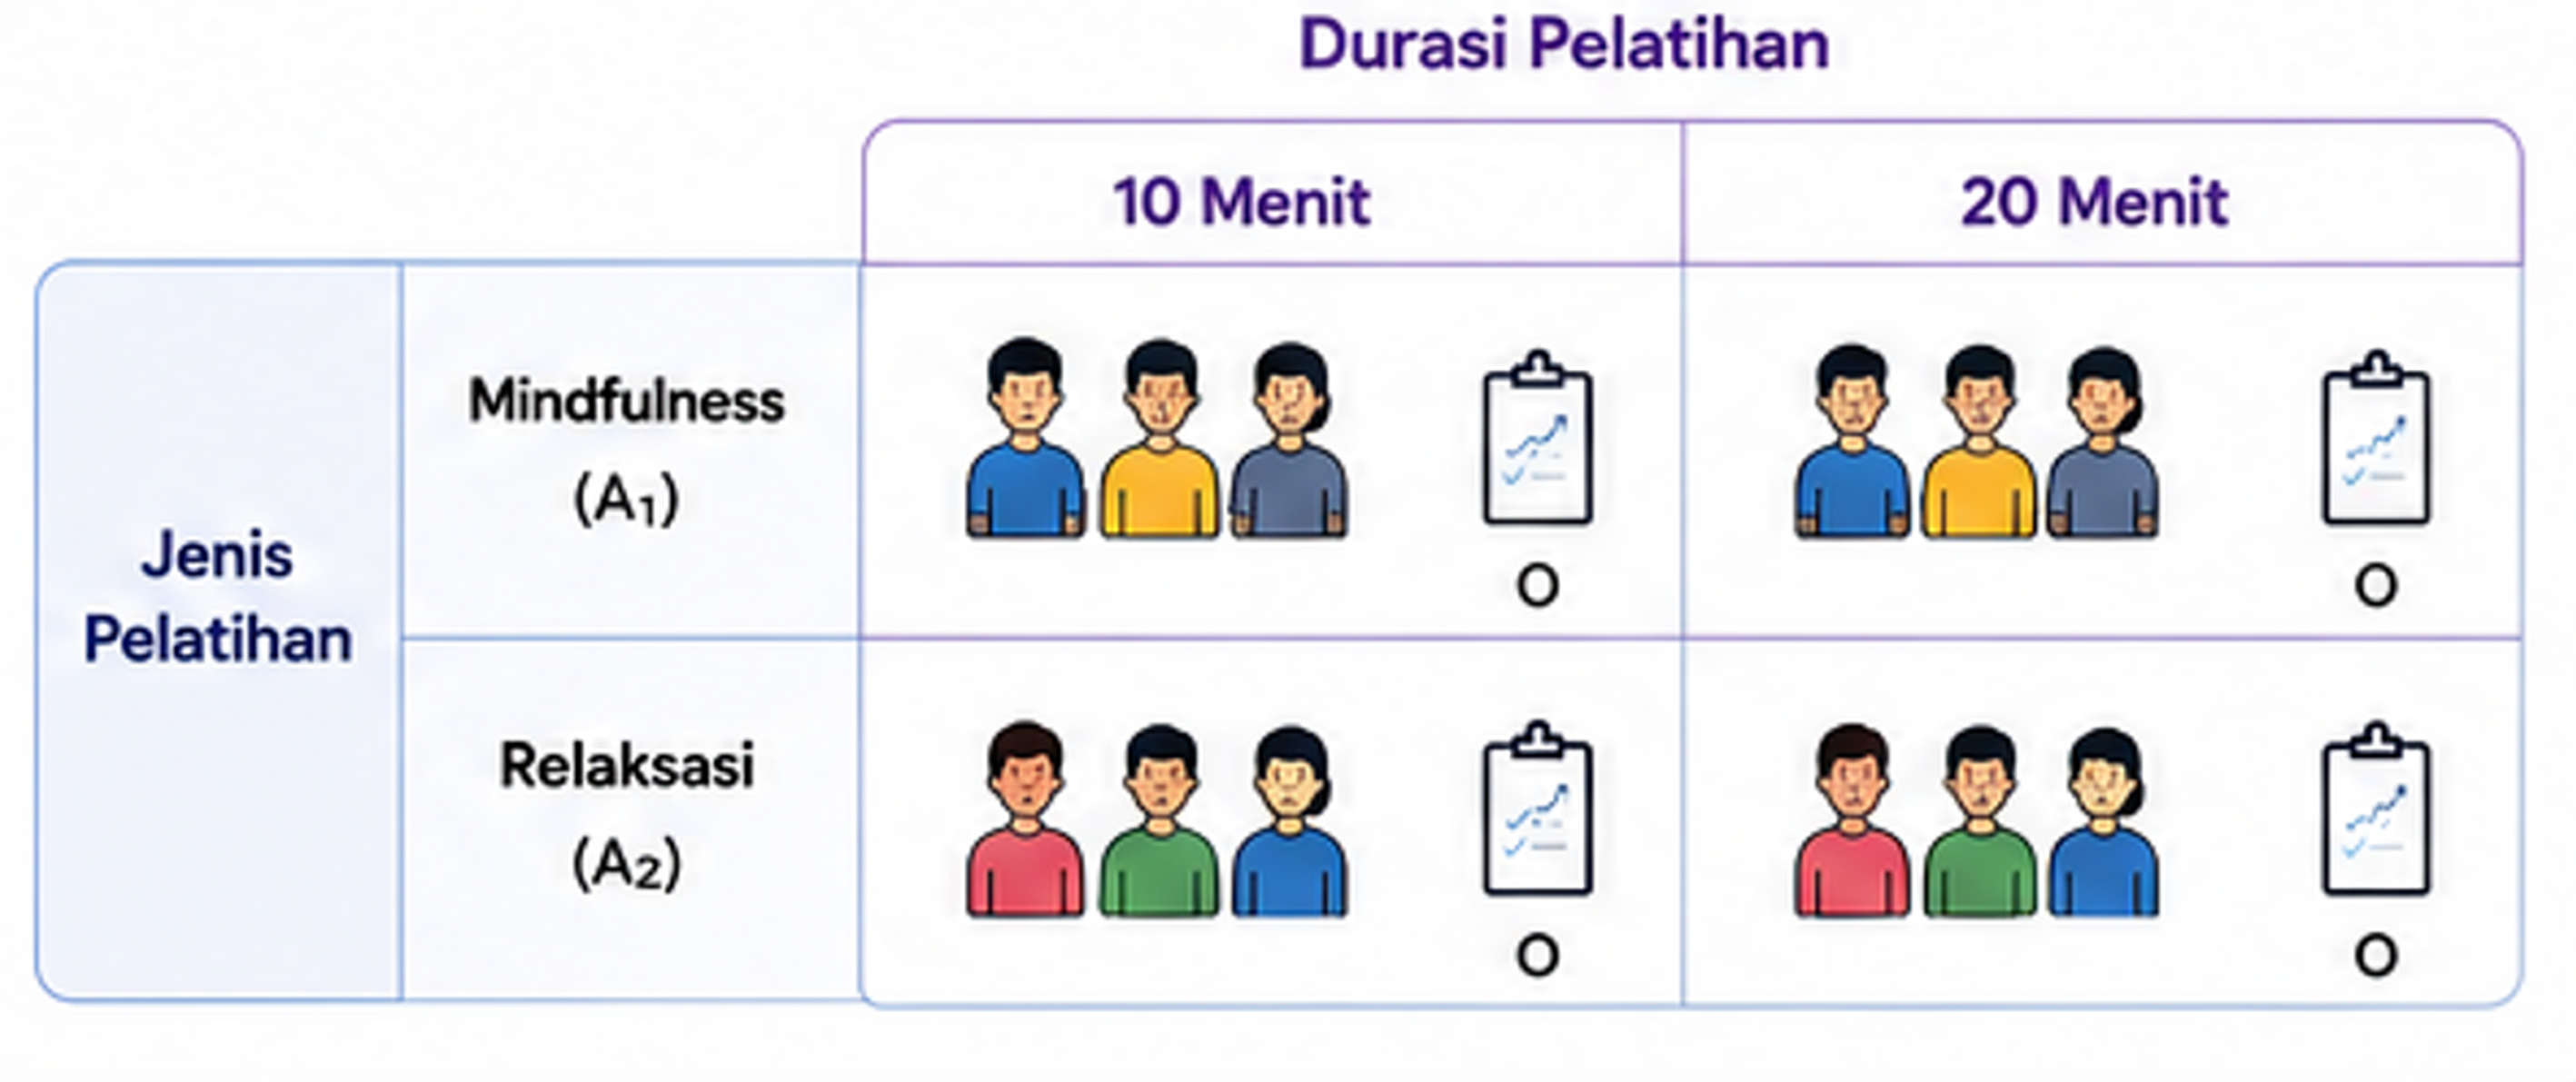
\includegraphics[keepaspectratio]{images/faktorial2.png}}

}

\caption{Ilustrasi desain faktorial}

\end{figure}%

Tabel~\ref{tbl-desainexp} merangkum karakteristik utama masing-masing
bentuk desain eksperimen sehingga memudahkan peneliti membandingkan
kelebihan dan penerapan setiap desain.

\begin{longtable}[]{@{}
  >{\raggedright\arraybackslash}p{(\linewidth - 8\tabcolsep) * \real{0.2000}}
  >{\centering\arraybackslash}p{(\linewidth - 8\tabcolsep) * \real{0.2000}}
  >{\centering\arraybackslash}p{(\linewidth - 8\tabcolsep) * \real{0.2000}}
  >{\centering\arraybackslash}p{(\linewidth - 8\tabcolsep) * \real{0.2000}}
  >{\centering\arraybackslash}p{(\linewidth - 8\tabcolsep) * \real{0.2000}}@{}}
\caption{Perbandingan karakteristik antar desain
eksperimen}\label{tbl-desainexp}\tabularnewline
\toprule\noalign{}
\endfirsthead
\endhead
\bottomrule\noalign{}
\endlastfoot
\textbf{Desain} & \textbf{Kelompok Pembanding} & \textbf{\emph{Pretest}}
& \textbf{\emph{Random Assignment}} & \textbf{Kegunaan} \\
\emph{One-shot case study} & ✗ & ✗ & ✗ & Studi awal \\
\emph{One-group pretest-posttest} & ✗ & ✓ & ✗ & Evaluasi awal \\
\emph{Static-group comparison} & ✓ & ✗ & ✗ & Perbandingan sederhana \\
\emph{Nonequivalent control group} & ✓ & ✓ & ✗ & Penelitian lapangan \\
\emph{Interrupted time series} & Tidak selalu & Berulang & ✗ & Evaluasi
kebijakan \\
\emph{Regression discontinuity} & ✓ & Berdasarkan \emph{cut-off} & ✗ &
Program selektif \\
\emph{Posttest-only} & ✓ & ✗ & ✓ & Menghindari efek \emph{pretest} \\
\emph{Pretest-posttest} & ✓ & ✓ & ✓ & Intervensi psikologi \\
\emph{Solomon four-group} & ✓ & Sebagian & ✓ & Menguji efek
\emph{pretest} \\
\emph{Factorial} & ✓ & Fleksibel & ✓ & Menguji lebih dari satu
perlakuan \\
\end{longtable}

\section{Validitas dan Etika dalam Penelitian
Eksperimen}\label{validitas-dan-etika-dalam-penelitian-eksperimen}

Pemilihan desain eksperimen yang tepat merupakan salah satu upaya untuk
meningkatkan kualitas penelitian. Dalam penelitian eksperimen, validitas
sangat dipengaruhi oleh kemampuan peneliti mengendalikan variabel luar
sehingga perubahan pada variabel dependen benar-benar berkaitan dengan
perlakuan yang diberikan. Oleh karena itu, penerapan manipulasi,
kelompok pembanding, \emph{random assignment}, serta prosedur penelitian
yang konsisten menjadi aspek penting dalam menghasilkan temuan yang
dapat dipercaya (Morling, 2024; Shadish dkk., 2002).

Selain itu, penelitian eksperimen harus dilaksanakan sesuai dengan
prinsip-prinsip etika penelitian. Peneliti perlu memperoleh
\emph{informed consent}, menjaga kerahasiaan data partisipan,
meminimalkan risiko yang mungkin timbul, memberikan kebebasan kepada
partisipan untuk mengundurkan diri kapan saja, serta melakukan
\emph{debriefing} apabila penelitian melibatkan penyamaran informasi
(\emph{deception}). Dengan memperhatikan validitas dan etika secara
bersamaan, penelitian eksperimen tidak hanya menghasilkan bukti ilmiah
yang kuat, tetapi juga tetap menghormati hak dan kesejahteraan
partisipan.

\begin{tcolorbox}[enhanced jigsaw, colframe=quarto-callout-tip-color-frame, toptitle=1mm, breakable, leftrule=.75mm, arc=.35mm, toprule=.15mm, colback=white, colbacktitle=quarto-callout-tip-color!10!white, bottomtitle=1mm, bottomrule=.15mm, titlerule=0mm, title=\textcolor{quarto-callout-tip-color}{\faLightbulb}\hspace{0.5em}{Rangkuman}, coltitle=black, left=2mm, opacitybacktitle=0.6, opacityback=0, rightrule=.15mm]

\begin{enumerate}
\def\labelenumi{\arabic{enumi}.}
\tightlist
\item
  Penelitian eksperimen merupakan desain penelitian yang digunakan untuk
  menguji hubungan sebab-akibat melalui manipulasi variabel independen
  dan pengamatan terhadap perubahan pada variabel dependen.
\item
  Berdasarkan tingkat kontrol terhadap variabel luar, desain eksperimen
  dibedakan menjadi eksperimen murni, kuasi eksperimen, dan
  pra-eksperimen. Ketiga desain tersebut memiliki karakteristik, tingkat
  validitas internal, serta kekuatan inferensi kausal yang berbeda.
\item
  Penelitian eksperimen dapat menggunakan \emph{between-subjects design}
  atau \emph{within-subjects design}, bergantung pada cara partisipan
  mengikuti kondisi eksperimen dan tujuan penelitian.
\item
  Pemilihan desain eksperimen harus mempertimbangkan keseimbangan antara
  kekuatan kontrol metodologis, kondisi lapangan, pertimbangan etika,
  ketersediaan sumber daya, serta tujuan penelitian.
\item
  Penelitian eksperimen harus dilaksanakan dengan memperhatikan
  validitas penelitian dan prinsip-prinsip etika agar menghasilkan
  temuan yang dapat dipercaya sekaligus melindungi hak dan kesejahteraan
  partisipan.
\end{enumerate}

\end{tcolorbox}

\begin{tcolorbox}[enhanced jigsaw, colframe=quarto-callout-important-color-frame, toptitle=1mm, breakable, leftrule=.75mm, arc=.35mm, toprule=.15mm, colback=white, colbacktitle=quarto-callout-important-color!10!white, bottomtitle=1mm, bottomrule=.15mm, titlerule=0mm, title=\textcolor{quarto-callout-important-color}{\faExclamation}\hspace{0.5em}{Refleksi \& Diskusi}, coltitle=black, left=2mm, opacitybacktitle=0.6, opacityback=0, rightrule=.15mm]

\begin{itemize}
\item
  Mengapa eksperimen dianggap lebih kuat daripada penelitian
  korelasional dalam menjelaskan hubungan sebab-akibat?
\item
  Apa perbedaan utama antara eksperimen murni, kuasi eksperimen, dan
  pra-eksperimen?

  Dalam situasi apa peneliti lebih tepat menggunakan kuasi eksperimen
  daripada eksperimen murni?
\item
  Apa perbedaan antara \emph{between-subjects design} dan
  \emph{within-subjects design}?
\item
  Apa saja pertimbangan etis yang perlu diperhatikan ketika peneliti
  memberikan perlakuan atau intervensi kepada partisipan?
\item
  Tentukan sebuah masalah penelitian di bidang psikologi, kemudian pilih
  desain eksperimen yang paling sesuai (pra-eksperimen, kuasi
  eksperimen, atau eksperimen murni). Jelaskan alasan pemilihan desain
  tersebut beserta bentuk rancangan eksperimen yang akan digunakan.
\end{itemize}

\end{tcolorbox}

\phantomsection\label{refs--12}
\begin{CSLReferences}{1}{0}
\bibitem[\citeproctext]{ref-Campbell1963--12}
Campbell, D. T., \& Stanley, J. (1963). \emph{Experimental and
Quasi-Experimental Designs for Research}. Cengage Learning.

\bibitem[\citeproctext]{ref-Creswell2018a--12}
Creswell, J. W., \& Creswell, J. D. (2023). \emph{Research design:
Qualitative, quantitative, and mixed methods approaches} (6th ed.). SAGE
Publications.

\bibitem[\citeproctext]{ref-Gravetter2018--12}
Gravetter, F. J., \& Forzano, L. B. (2018). \emph{Research Methods for
the Behavioral Sciences} (6th ed.). Cengage Learning EMEA (UK; Europe).

\bibitem[\citeproctext]{ref-Jhangiani2019--12}
Jhangiani, R., Chiang, I.-C. A., Cuttler, C., \& Leighton, D. C. (2019).
\emph{Research methods in psychology}. Kwantlen Polytechnic University.

\bibitem[\citeproctext]{ref-Morling2024--12}
Morling, B. (2024). \emph{Research methods in psychology : evaluating a
world of information} (4th ed.). W.W. Norton \& Company, Inc.

\bibitem[\citeproctext]{ref-Shadish2002--12}
Shadish, W. R., Cook, T. D., \& Campbell, D. T. (2002).
\emph{Experimental and quasi-experimental designs for generalized causal
inference} (2nd ed.). Wadsworth/Cengage Learning.

\end{CSLReferences}

\chapter{Desain Korelasional \&
Survei}\label{desain-korelasional-survei}

\begin{tcolorbox}[enhanced jigsaw, colframe=quarto-callout-note-color-frame, toptitle=1mm, breakable, leftrule=.75mm, arc=.35mm, toprule=.15mm, colback=white, colbacktitle=quarto-callout-note-color!10!white, bottomtitle=1mm, bottomrule=.15mm, titlerule=0mm, title=\textcolor{quarto-callout-note-color}{\faInfo}\hspace{0.5em}{Capaian Pembelajaran}, coltitle=black, left=2mm, opacitybacktitle=0.6, opacityback=0, rightrule=.15mm]

Setelah mempelajari bab ini, mahasiswa diharapkan mampu:

\begin{enumerate}
\def\labelenumi{\arabic{enumi}.}
\tightlist
\item
  Menjelaskan konsep, tujuan, dan karakteristik utama desain
  korelasional dan desain survei.
\item
  Membedakan desain korelasional dan desain survei berdasarkan tujuan
  penelitian, jenis pertanyaan penelitian, metode pengumpulan data,
  serta luaran penelitian.
\item
  Menentukan desain penelitian yang paling sesuai berdasarkan tujuan
  penelitian dan rumusan masalah yang diajukan.
\item
  Mengidentifikasi contoh penerapan desain korelasional dan desain
  survei dalam berbagai topik penelitian psikologi maupun ilmu sosial.
\end{enumerate}

\end{tcolorbox}

Dalam penelitian kuantitatif, tidak semua pertanyaan penelitian
bertujuan menguji pengaruh atau hubungan sebab-akibat melalui
eksperimen. Pada banyak kasus, peneliti hanya ingin mengetahui apakah
terdapat hubungan antara dua atau lebih variabel, atau memperoleh
gambaran mengenai karakteristik suatu populasi tanpa memberikan
perlakuan apa pun. Untuk tujuan tersebut, tersedia berbagai desain
penelitian non-eksperimental, di antaranya desain korelasional dan
desain survei.

Kedua desain tersebut sama-sama dilakukan pada kondisi alamiah tanpa
manipulasi variabel dan sering kali menggunakan kuesioner sebagai
instrumen pengumpulan data. Kesamaan ini menyebabkan desain korelasional
dan desain survei kerap dianggap sebagai desain yang sama, padahal
keduanya memiliki tujuan, fokus analisis, dan hasil yang berbeda. Oleh
karena itu, bab ini membahas konsep dasar, karakteristik, serta
perbedaan antara desain korelasional dan desain survei agar pembaca
dapat memilih desain yang paling sesuai dengan tujuan penelitiannya.

\section{Desain Korelasional}\label{desain-korelasional}

\subsection{Pengertian}\label{pengertian}

Desain korelasional merupakan salah satu desain penelitian kuantitatif
non-eksperimental yang bertujuan untuk mengkaji hubungan antara dua atau
lebih variabel tanpa memberikan perlakuan atau manipulasi terhadap
variabel yang diteliti (Creswell \& Creswell, 2023). Dalam desain ini,
peneliti mengamati variabel sebagaimana adanya pada kondisi alamiah,
kemudian menganalisis apakah perubahan pada suatu variabel berkaitan
dengan perubahan pada variabel lainnya.

Perlu dipahami bahwa hubungan yang ditemukan dalam penelitian
korelasional tidak menunjukkan adanya hubungan sebab-akibat. Hal ini
karena peneliti tidak mengendalikan variabel luar maupun memanipulasi
variabel independen sebagaimana dilakukan pada penelitian eksperimen
(Johnson \& Christensen, 2020). Oleh sebab itu, hasil penelitian
korelasional hanya dapat menunjukkan adanya keterkaitan antarvariabel,
bukan membuktikan bahwa satu variabel menyebabkan perubahan pada
variabel lainnya.

Istilah \emph{desain korelasional} berasal dari teknik analisis
statistik yang digunakan, yaitu analisis korelasi. Hasil analisis
tersebut dinyatakan dalam bentuk koefisien korelasi yang menggambarkan
arah dan kekuatan hubungan antarvariabel.

\subsection{Tujuan}\label{tujuan}

Tujuan utama desain korelasional adalah mengidentifikasi dan mengukur
hubungan antara dua atau lebih variabel. Hubungan tersebut dinyatakan
dalam bentuk koefisien korelasi yang menunjukkan \textbf{arah} hubungan
(positif atau negatif) dan \textbf{kekuatan} hubungan (lemah hingga
kuat) (Creswell \& Creswell, 2023).

Suatu hubungan dikatakan ada apabila perubahan pada satu variabel
cenderung diikuti oleh perubahan pada variabel lain secara konsisten.
Sebaliknya, apabila perubahan pada satu variabel tidak berkaitan dengan
perubahan pada variabel lainnya, maka kedua variabel tersebut dikatakan
tidak memiliki hubungan. Dengan kata lain, penelitian korelasional
berusaha mengidentifikasi apakah variasi skor pada suatu variabel
berkaitan dengan variasi skor pada variabel lain.

Secara umum, desain korelasional digunakan untuk:

\begin{enumerate}
\def\labelenumi{\arabic{enumi}.}
\tightlist
\item
  Menguji apakah terdapat hubungan antara dua atau lebih variabel.
\item
  Menentukan arah hubungan, yaitu hubungan positif atau negatif.
\item
  Mengetahui kekuatan hubungan antarvariabel.
\item
  Menilai signifikansi statistik dari hubungan yang ditemukan.
\item
  Menjadi dasar untuk mengembangkan model prediksi atau penelitian
  lanjutan, termasuk penelitian eksperimen, apabila diperlukan.
\end{enumerate}

\subsection{Pengumpulan Data}\label{pengumpulan-data}

Pada penelitian korelasional, pengumpulan data bertujuan memperoleh
informasi mengenai seluruh variabel yang akan dianalisis hubungan di
antaranya. Oleh karena itu, setiap variabel harus diukur pada unit
analisis yang sama sehingga hubungan antarvariabel dapat dianalisis.
Peneliti dapat memilih teknik pengumpulan data yang paling sesuai dengan
karakteristik variabel dan sumber data yang tersedia (Fraenkel dkk.,
2023; Johnson \& Christensen, 2020).

Beberapa teknik pengumpulan data yang umum digunakan dalam penelitian
korelasional adalah sebagai berikut.

\begin{enumerate}
\def\labelenumi{\arabic{enumi}.}
\tightlist
\item
  \textbf{Kuesioner atau skala psikologis.} Teknik ini banyak digunakan
  apabila variabel yang diteliti berupa konstruk psikologis, seperti
  sikap, kepribadian, stres, kecemasan, kepuasan hidup, atau motivasi.
  Setiap partisipan diminta memberikan respons terhadap seperangkat
  pertanyaan atau pernyataan sehingga diperoleh skor untuk masing-masing
  variabel yang akan dianalisis.
\item
  \textbf{Observasi.} Apabila variabel yang diteliti berupa perilaku
  yang dapat diamati secara langsung, peneliti dapat menggunakan pedoman
  observasi. Sebagai contoh, peneliti dapat mengamati hubungan antara
  frekuensi interaksi guru dengan siswa dan tingkat partisipasi siswa
  selama proses pembelajaran.
\item
  \textbf{Dokumentasi atau data arsip.} Penelitian korelasional juga
  dapat memanfaatkan data yang telah tersedia, seperti nilai akademik,
  rekam medis, data administrasi, atau hasil pengukuran sebelumnya
  (Babbie, 2021). Misalnya, seorang peneliti ingin mengetahui hubungan
  antara nilai ujian masuk perguruan tinggi dengan indeks prestasi
  kumulatif (IPK) mahasiswa. Dalam penelitian tersebut, kedua variabel
  dapat diperoleh dari data akademik tanpa perlu melakukan pengukuran
  ulang.
\end{enumerate}

Dalam praktiknya, peneliti juga dapat mengombinasikan beberapa teknik
pengumpulan data apabila variabel yang diteliti berasal dari sumber yang
berbeda. Sebagai contoh, tingkat kecemasan dapat diukur menggunakan
skala psikologis, sedangkan prestasi akademik diperoleh dari data arsip
universitas. Selama setiap variabel berasal dari partisipan yang sama,
data tersebut dapat digunakan untuk mengkaji hubungan antarvariabel.

Perlu diperhatikan bahwa pemilihan teknik pengumpulan data tidak
menentukan apakah suatu penelitian termasuk desain korelasional atau
bukan. Desain penelitian ditentukan oleh tujuan penelitian, yaitu
mengkaji hubungan antarvariabel, sedangkan teknik pengumpulan data
dipilih berdasarkan jenis variabel yang akan diukur dan ketersediaan
sumber data (Creswell \& Creswell, 2023). Contoh penerapan desain
korelasional mulai dari identifikasi fenomena hingga pemilihan desain
penelitian dapat dilihat pada Gambar~\ref{fig-korelasional}.

\begin{figure}

\centering{

\begin{figure}
\centering
\pandocbounded{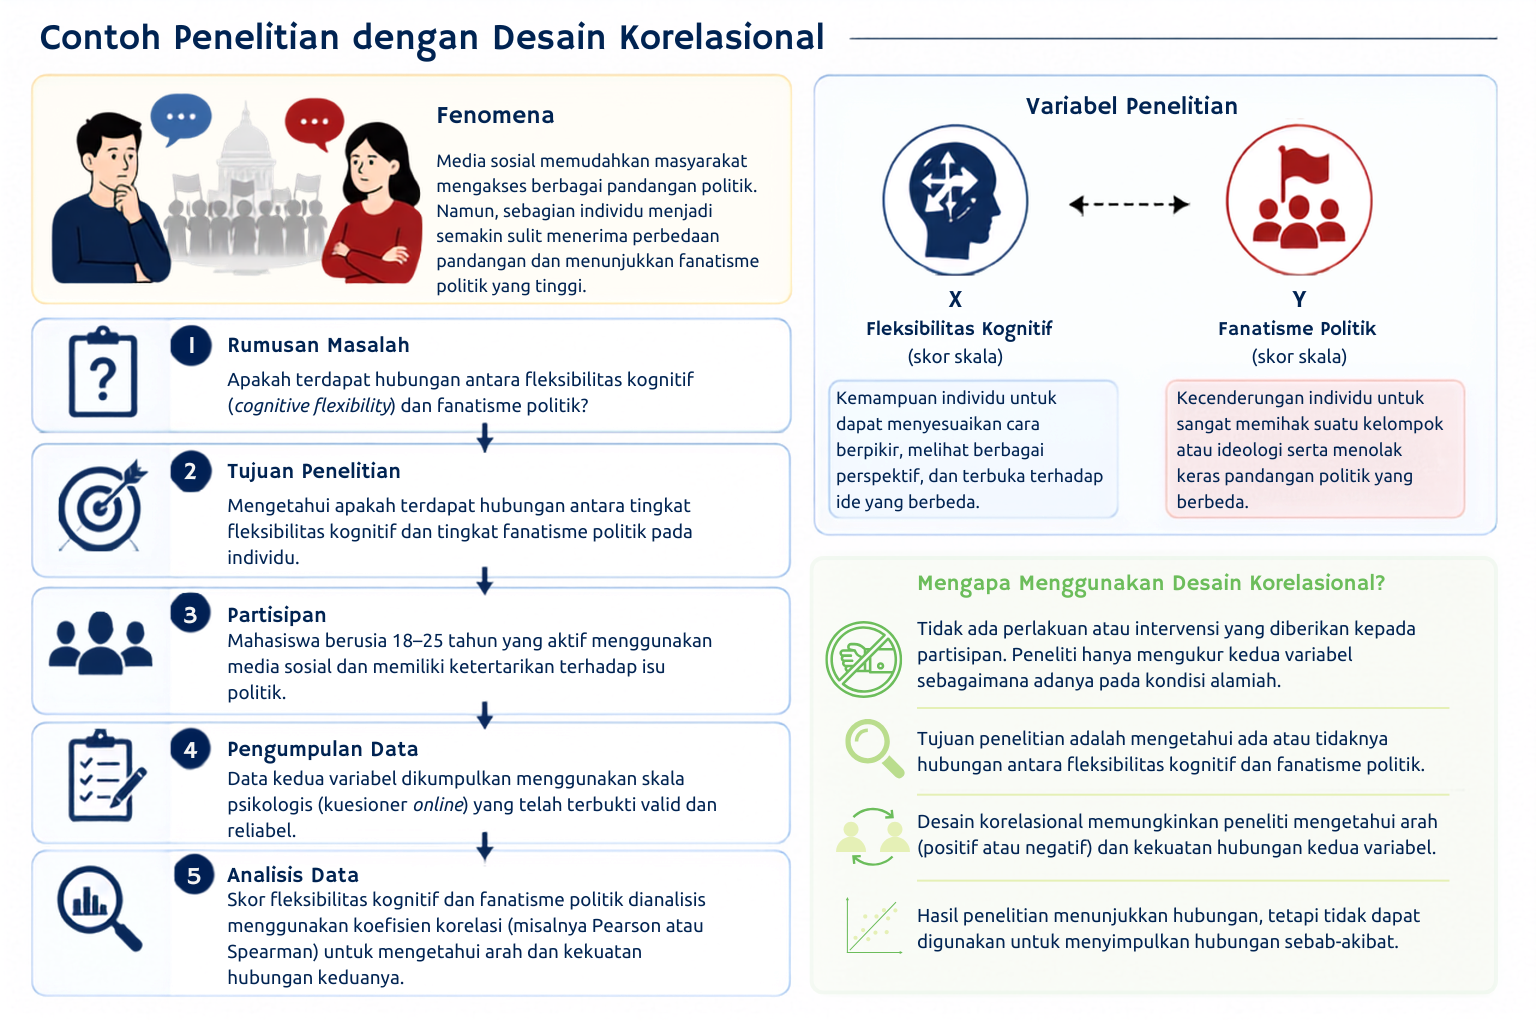
\includegraphics[keepaspectratio]{images/korelasional.png}}
\caption{Contoh Penelitian Menggunakan Desain Korelasional}
\end{figure}

}

\caption{\label{fig-korelasional}}

\end{figure}%

\subsection{Keunggulan \& Keterbatasan}\label{keunggulan-keterbatasan}

Keunggulan dan keterbatasan desain penelitian korelasional dapat
dibandingkan secara ringkas melalui Tabel~\ref{tbl-korelasional}.

\begin{longtable}[]{@{}
  >{\raggedright\arraybackslash}p{(\linewidth - 2\tabcolsep) * \real{0.5000}}
  >{\raggedright\arraybackslash}p{(\linewidth - 2\tabcolsep) * \real{0.5000}}@{}}
\caption{Keunggulan dan keterbatasan desain
korelasional}\label{tbl-korelasional}\tabularnewline
\toprule\noalign{}
\begin{minipage}[b]{\linewidth}\raggedright
\textbf{Keunggulan}
\end{minipage} & \begin{minipage}[b]{\linewidth}\raggedright
\textbf{Keterbatasan}
\end{minipage} \\
\midrule\noalign{}
\endfirsthead
\toprule\noalign{}
\begin{minipage}[b]{\linewidth}\raggedright
\textbf{Keunggulan}
\end{minipage} & \begin{minipage}[b]{\linewidth}\raggedright
\textbf{Keterbatasan}
\end{minipage} \\
\midrule\noalign{}
\endhead
\bottomrule\noalign{}
\endlastfoot
Lebih efisien karena tidak memerlukan manipulasi variabel atau pemberian
perlakuan. & Tidak dapat digunakan untuk menyimpulkan hubungan
sebab--akibat. \\
Data dikumpulkan pada kondisi alami sehingga memiliki validitas ekologis
yang relatif tinggi. & Rentan terhadap pengaruh variabel perancu
(\emph{confounding variables}) yang tidak diukur. \\
Dapat digunakan untuk meneliti variabel yang sulit atau tidak etis
dimanipulasi secara eksperimen. & Tidak dapat memastikan arah hubungan
antarvariabel. \\
Mampu menganalisis hubungan antara banyak variabel sekaligus dengan
berbagai teknik analisis korelasional. & Korelasi yang signifikan secara
statistik belum tentu memiliki makna praktis yang besar. \\
\end{longtable}

\section{Desain Survey}\label{desain-survey}

\subsection{Pengertian}\label{pengertian-1}

Desain survei (\emph{survey design}) adalah desain penelitian
kuantitatif yang digunakan untuk mengumpulkan data dari sampel guna
menggambarkan karakteristik, sikap, opini, perilaku, atau kondisi suatu
populasi. Hasil yang diperoleh dari sampel kemudian digunakan untuk
mengestimasi karakteristik populasi yang lebih luas (Creswell \&
Creswell, 2023; Fraenkel dkk., 2023).

Seperti desain korelasional, dalam desain survei peneliti tidak
memberikan perlakuan maupun memanipulasi variabel yang diteliti. Data
dikumpulkan sebagaimana adanya dari responden menggunakan instrumen yang
terstandarisasi. Perlu dipahami bahwa survei merupakan desain
penelitian, sedangkan kuesioner hanyalah salah satu instrumen yang dapat
digunakan untuk mengumpulkan data dalam penelitian survei (Babbie,
2021).

Berbeda dengan \textbf{desain korelasional} yang berfokus pada pengujian
hubungan antarvariabel, \textbf{desain survei} berfokus pada pengumpulan
informasi untuk menggambarkan karakteristik suatu populasi. Meskipun
data survei dapat dianalisis menggunakan teknik korelasional, tujuan
utama penelitian survei bukanlah menguji hubungan antarvariabel,
melainkan mendeskripsikan kondisi atau karakteristik populasi yang
diteliti (Creswell \& Creswell, 2023).

\subsection{Tujuan}\label{tujuan-1}

Desain survei digunakan ketika peneliti ingin memperoleh informasi
mengenai karakteristik suatu populasi berdasarkan data yang dikumpulkan
dari sampel. Bergantung pada tujuan penelitian, survei dapat
dimanfaatkan untuk mendeskripsikan suatu fenomena, mengukur
karakteristik populasi, maupun membandingkan karakteristik antar
kelompok (Creswell \& Creswell, 2023; Privitera, 2020). Secara umum,
tujuan penggunaan desain survei meliputi hal-hal berikut:

\begin{enumerate}
\def\labelenumi{\arabic{enumi}.}
\tightlist
\item
  Menggambarkan karakteristik suatu populasi
\item
  Mengukur sikap, opini, persepsi, atau perilaku responden
\item
  Mengestimasi prevalensi atau distribusi suatu fenomena
\item
  Membandingkan karakteristik antar kelompok
\item
  Menyediakan dasar bagi pengambilan keputusan
\end{enumerate}

\subsection{Pengumpulan Data}\label{pengumpulan-data-1}

Dalam penelitian survei, data dikumpulkan secara sistematis dari
sejumlah responden menggunakan instrumen yang terstandarisasi. Instrumen
yang paling umum digunakan adalah kuesioner, meskipun wawancara
terstruktur juga dapat digunakan sesuai dengan tujuan dan karakteristik
responden.

Survei dapat dilaksanakan secara tatap muka, melalui telepon, melalui
pos, maupun secara daring (\emph{online survey}). Pemilihan metode
pengumpulan data perlu mempertimbangkan karakteristik populasi,
ketersediaan sumber daya, serta kemudahan akses responden.

Agar hasil survei dapat menggambarkan kondisi populasi secara akurat,
peneliti perlu menggunakan instrumen yang valid dan reliabel, memilih
sampel yang representatif, serta mengupayakan tingkat respons
(\emph{response rate}) yang memadai untuk meminimalkan potensi
\emph{nonresponse bias} (Fraenkel dkk., 2023). Contoh penerapan desain
survei mulai dari identifikasi fenomena hingga pemilihan desain
penelitian dapat dilihat pada Gambar~\ref{fig-survei}.

\begin{figure}

\centering{

\begin{figure}
\centering
\pandocbounded{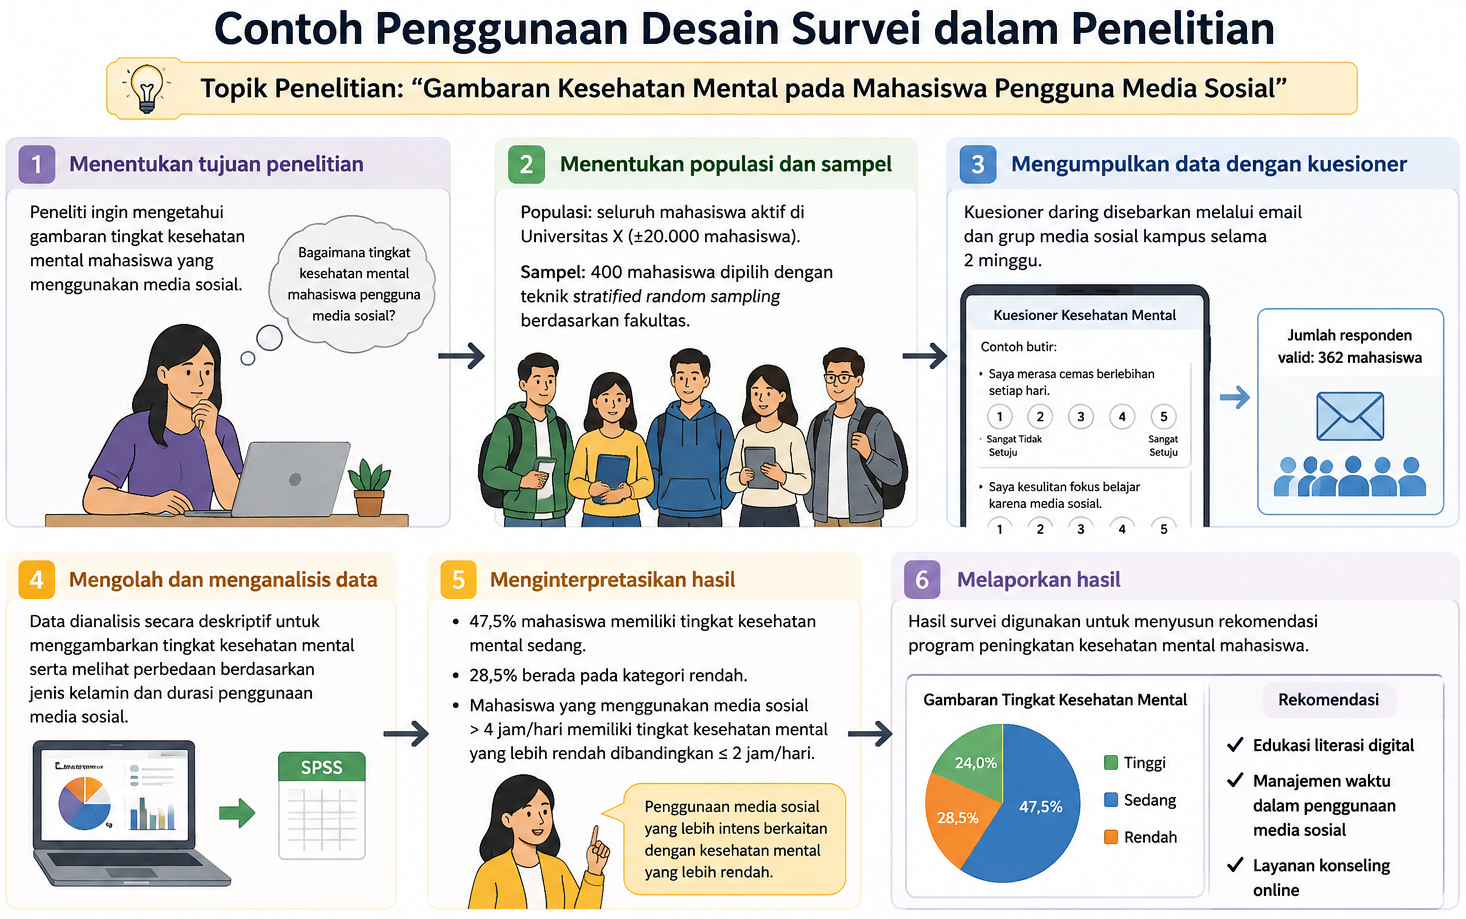
\includegraphics[keepaspectratio]{images/survei.png}}
\caption{Contoh penelitian dengan desain survei}
\end{figure}

}

\caption{\label{fig-survei}}

\end{figure}%

\subsection{Keunggulan \& Keterbatasan}\label{keunggulan-keterbatasan-1}

Keunggulan dan keterbatasan desain survei dapat dibandingkan secara
ringkas dalam Tabel~\ref{tbl-survei} .

\begin{longtable}[]{@{}
  >{\raggedright\arraybackslash}p{(\linewidth - 2\tabcolsep) * \real{0.4722}}
  >{\raggedright\arraybackslash}p{(\linewidth - 2\tabcolsep) * \real{0.5278}}@{}}
\caption{Keunggulan dan keterbatasan desain
survei}\label{tbl-survei}\tabularnewline
\toprule\noalign{}
\endfirsthead
\endhead
\bottomrule\noalign{}
\endlastfoot
\textbf{Keunggulan} & \textbf{Keterbatasan} \\
Mampu mengumpulkan data dari banyak responden dalam waktu yang relatif
singkat. & Tidak dapat digunakan untuk menyimpulkan hubungan
sebab--akibat. \\
Efisien dari segi biaya dan pelaksanaan, terutama melalui survei daring
(\emph{online survey}). & Kualitas data sangat bergantung pada kejujuran
dan pemahaman responden. \\
Hasil penelitian dapat digeneralisasikan apabila menggunakan sampel yang
representatif. & Rentan terhadap \emph{response bias} dan
\emph{nonresponse bias}. \\
Dapat mengukur berbagai karakteristik, sikap, opini, dan perilaku secara
bersamaan menggunakan instrumen yang terstandarisasi. & Kesalahan dalam
penyusunan instrumen atau teknik sampling dapat menurunkan validitas
hasil penelitian. \\
\end{longtable}

\section{Perbandingan Desain Korelasional dan Desain
Survei}\label{perbandingan-desain-korelasional-dan-desain-survei}

Desain korelasional dan desain survei sama-sama termasuk dalam
penelitian kuantitatif non-eksperimental karena peneliti tidak
memberikan perlakuan maupun memanipulasi variabel penelitian. Keduanya
juga sering menggunakan kuesioner sebagai instrumen pengumpulan data.
Meskipun demikian, kedua desain memiliki tujuan yang berbeda. Desain
korelasional berfokus pada pengujian hubungan antarvariabel, sedangkan
desain survei bertujuan memperoleh gambaran mengenai karakteristik suatu
populasi berdasarkan data yang dikumpulkan dari sampel (Creswell \&
Creswell, 2023; Privitera, 2020) (lihat Tabel~\ref{tbl-korelvssurvei}).

\begin{longtable}[]{@{}
  >{\raggedright\arraybackslash}p{(\linewidth - 4\tabcolsep) * \real{0.2639}}
  >{\raggedright\arraybackslash}p{(\linewidth - 4\tabcolsep) * \real{0.3472}}
  >{\raggedright\arraybackslash}p{(\linewidth - 4\tabcolsep) * \real{0.3889}}@{}}
\caption{Perbandingan desain korelasi dan
survei}\label{tbl-korelvssurvei}\tabularnewline
\toprule\noalign{}
\endfirsthead
\endhead
\bottomrule\noalign{}
\endlastfoot
\textbf{Aspek} & \textbf{Desain Korelasional} & \textbf{Desain
Survei} \\
Tujuan utama & Menguji hubungan antara dua atau lebih variabel. &
Menggambarkan karakteristik, sikap, opini, atau perilaku suatu
populasi. \\
Fokus penelitian & Hubungan antarvariabel. & Karakteristik populasi. \\
Pertanyaan penelitian & \emph{Apakah terdapat hubungan antara variabel X
dan Y?} & \emph{Bagaimana karakteristik populasi yang diteliti?} \\
Jumlah variabel & Minimal 2 & Minimal 1 \\
Analisis utama & Korelasi (\emph{Pearson}, \emph{Spearman}), regresi,
atau analisis hubungan lainnya. & Statistik deskriptif, seperti
frekuensi, persentase, rata-rata, dan distribusi data. \\
Hasil penelitian & Menunjukkan arah dan kekuatan hubungan antarvariabel.
& Memberikan gambaran kondisi atau karakteristik populasi. \\
Contoh topik & Hubungan antara \emph{cognitive flexibility} dan
fanatisme politik. & Gambaran tingkat literasi \emph{artificial
intelligence} pada mahasiswa Indonesia. \\
\end{longtable}

Perbedaan tersebut tidak berarti bahwa kedua desain tidak dapat
digunakan secara bersamaan. Sebagai contoh, seorang peneliti dapat
mengumpulkan data menggunakan desain survei, kemudian menganalisis
hubungan antarvariabel dalam data tersebut menggunakan analisis
korelasional. Dalam kondisi seperti ini, survei menggambarkan cara
pengumpulan data, sedangkan korelasional menggambarkan tujuan analisis
data. Oleh karena itu, peneliti perlu menjelaskan secara jelas apakah
istilah ``survei'' merujuk pada desain penelitian, metode pengumpulan
data, atau konteks pelaksanaan penelitian agar tidak menimbulkan
ambiguitas (Babbie, 2021).

\section{Memilih Desain Penelitian yang
Tepat}\label{memilih-desain-penelitian-yang-tepat}

Pemilihan desain penelitian harus disesuaikan dengan tujuan dan
pertanyaan penelitian. Meskipun sama-sama termasuk penelitian
kuantitatif non-eksperimental, desain korelasional dan desain survei
memiliki fokus yang berbeda. Gambar~\ref{fig-korelvssurvei} dapat
digunakan sebagai panduan dalam memilih desain yang paling sesuai.

\begin{figure}

\centering{

\pandocbounded{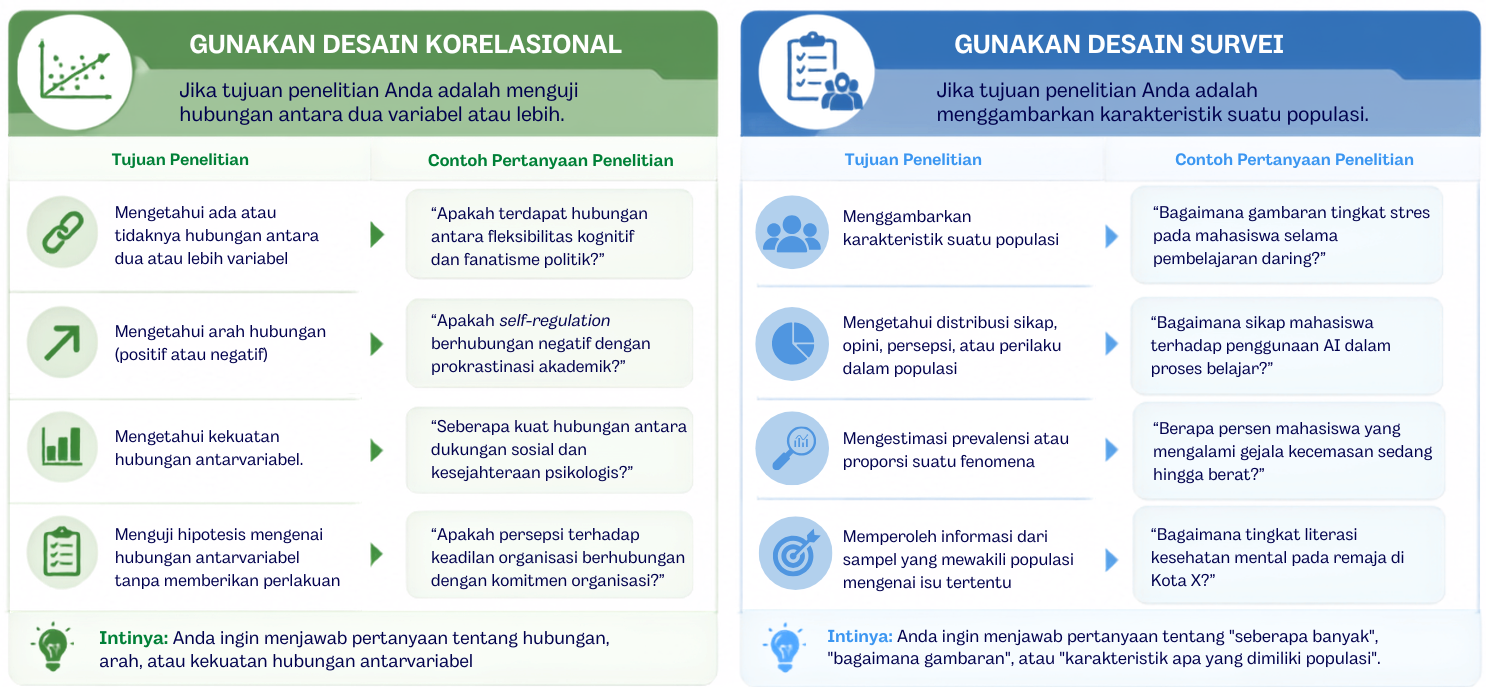
\includegraphics[keepaspectratio]{images/korelasivssurvei.png}}

}

\caption{\label{fig-korelvssurvei}}

\end{figure}%

\phantomsection\label{refs--13}
\begin{CSLReferences}{1}{0}
\bibitem[\citeproctext]{ref-Babbie2021--13}
Babbie, E. (2021). \emph{The practice of social research} (15th ed.).
Cengage Learning.

\bibitem[\citeproctext]{ref-Creswell2018a--13}
Creswell, J. W., \& Creswell, J. D. (2023). \emph{Research design:
Qualitative, quantitative, and mixed methods approaches} (6th ed.). SAGE
Publications.

\bibitem[\citeproctext]{ref-Fraenkel2023--13}
Fraenkel, J. R., Wallen, N. E., \& Hyun, H. H. (2023). \emph{How to
design and evaluate research in education}. McGraw Hill LLC.

\bibitem[\citeproctext]{ref-Johnson2020--13}
Johnson, B., \& Christensen, L. B. (2020). \emph{Educational research :
quantitative, qualitative, and mixed approaches}. SAGE Publications,
Inc.

\bibitem[\citeproctext]{ref-Privitera2020--13}
Privitera, G. J. (2020). \emph{Research methods for the behavioral
sciences} (3rd ed.). Sage Publications, Inc.

\end{CSLReferences}

\chapter{Perancangan Penelitian
Kuantitatif}\label{perancangan-penelitian-kuantitatif}

\begin{tcolorbox}[enhanced jigsaw, colframe=quarto-callout-note-color-frame, toptitle=1mm, breakable, leftrule=.75mm, arc=.35mm, toprule=.15mm, colback=white, colbacktitle=quarto-callout-note-color!10!white, bottomtitle=1mm, bottomrule=.15mm, titlerule=0mm, title=\textcolor{quarto-callout-note-color}{\faInfo}\hspace{0.5em}{Capaian Pembelajaran}, coltitle=black, left=2mm, opacitybacktitle=0.6, opacityback=0, rightrule=.15mm]

Setelah mempelajari bab ini, mahasiswa diharapkan mampu:

\begin{enumerate}
\def\labelenumi{\arabic{enumi}.}
\tightlist
\item
  Menjelaskan tujuan dan fungsi proposal penelitian dalam proses
  penelitian kuantitatif.
\item
  Mengidentifikasi dan menjelaskan komponen-komponen utama yang terdapat
  dalam proposal penelitian kuantitatif.
\item
  Menyusun bagian-bagian proposal penelitian kuantitatif sesuai dengan
  kaidah penulisan ilmiah.
\item
  Menjelaskan keterkaitan antara permasalahan penelitian, tujuan
  penelitian, hipotesis, instrumen penelitian, dan rencana analisis
  data.
\item
  Mengevaluasi konsistensi dan kelayakan suatu proposal penelitian
  kuantitatif.
\item
  Menerapkan prinsip-prinsip penyusunan proposal penelitian untuk
  merancang penelitian kuantitatif yang sistematis dan realistis.
\end{enumerate}

\end{tcolorbox}

Pada bab-bab sebelumnya telah dibahas berbagai komponen utama penelitian
kuantitatif, mulai dari perumusan masalah penelitian, penyusunan
hipotesis, identifikasi variabel, pemilihan instrumen, hingga teknik
pengambilan sampel. Namun, dalam praktik penelitian, komponen-komponen
tersebut tidak berdiri sendiri. Seorang peneliti perlu
mengintegrasikannya ke dalam sebuah rancangan penelitian yang sistematis
dan realistis untuk dilaksanakan. Rancangan tersebut biasanya dituangkan
dalam bentuk proposal penelitian yang menjadi pedoman selama proses
penelitian berlangsung.

Proposal penelitian tidak hanya menjelaskan apa yang akan diteliti,
tetapi juga bagaimana penelitian akan dilakukan dan mengapa pendekatan
tertentu dipilih. Oleh karena itu, kemampuan menyusun proposal
penelitian merupakan salah satu kompetensi penting yang harus dikuasai
oleh mahasiswa dan peneliti. Bab ini membahas struktur proposal
penelitian kuantitatif, fungsi setiap komponennya, serta cara menyusun
proposal yang sistematis, logis, dan sesuai dengan kaidah ilmiah.

\section{Tujuan Proposal Penelitian}\label{tujuan-proposal-penelitian}

Proposal penelitian merupakan dokumen penting dalam setiap penelitian,
baik kualitatif maupun kuantitatif. Proposal ini berfungsi sebagai
rancangan yang menjelaskan tujuan, strategi, dan langkah operasional
untuk menjawab pertanyaan atau masalah penelitian (Kumar, 2018). Di
dalamnya, peneliti perlu menguraikan aktivitas yang akan dilakukan,
seperti menguji hipotesis dalam penelitian kuantitatif atau mencari
jawaban atas pertanyaan penelitian kualitatif, serta menyampaikan alasan
dilakukannya penelitian.

Fungsi utama proposal adalah memastikan metodologi yang digunakan valid
dan objektif, sekaligus meyakinkan pembaca mengenai kelayakan penelitian
(Creswell \& Creswell, 2023). Dengan demikian, proposal penelitian
menjadi dasar evaluasi dan penentu keberlanjutan suatu penelitian.
Secara garis besar, sebuah proposal perlu memiliki:

\begin{itemize}
\tightlist
\item
  Tujuan penelitian yang jelas.
\item
  Rencana operasional dan detail untuk memperoleh jawaban atas
  pertanyaan penelitian.
\item
  Alasan atau rasionalisasi dari setiap rencana dan strategi yang
  dipilih.
\end{itemize}

Proposal penelitian yang dibuat seharusnya dapat menjadi panduan dalam
melakukan penelitian, meyakinkan pembimbing dan penguji proposal
penelitian, atau pemberi hibah penelitian.

\section{Struktur Proposal
Penelitian}\label{struktur-proposal-penelitian}

Format proposal penelitian bisa berbeda dalam hal tata cara atau konten
penulisan, sesuai dengan institusi, disiplin ilmu atau tujuan pembuatan
proposal. Secara garis besar, sebuah proposal penelitian memuat sejumlah
informasi berikut:

\begin{enumerate}
\def\labelenumi{\arabic{enumi}.}
\tightlist
\item
  \textbf{Pendahuluan}, termasuk tinjauan pustaka singkat;
\item
  \textbf{Kerangka teoritis} dan konseptual yang mendasari studi;
\item
  \textbf{Tujuan} atau \textbf{pertanyaan penelitian} studi;
\item
  \textbf{Hipotesis} yang akan diuji;
\item
  \textbf{Desain penelitian} yang diusulkan untuk menjawab pertanyaan
  penelitian;
\item
  \textbf{Instrumen} penelitian yang akan digunakan;
\item
  \textbf{Teknik sampling} dan ukuran/jumlah sampel;
\item
  \textbf{Prosedur} perolehan dan pengolahan data;
\item
  \textbf{Kerangka waktu} yang diusulkan untuk menyelesaikan penelitian
  tersebut.
\end{enumerate}

\subsection{Pendahuluan}\label{pendahuluan-2}

Pendahuluan proposal penelitian disusun berdasarkan tinjauan literatur
yang relevan dengan masalah penelitian. Bagian ini dimulai dengan
penjelasan umum mengenai topik, lalu secara bertahap mengerucut pada
fokus atau isu utama yang diteliti. Pendahuluan yang baik biasanya
memuat:

\begin{itemize}
\tightlist
\item
  Gambaran umum topik penelitian;
\item
  Perspektif historis yang relevan dengan bidang studi;
\item
  Isu filosofis atau ideologis terkait topik;
\item
  Tren prevalensi (jika sesuai);
\item
  Teori-teori utama yang mendukung;
\item
  Isu, masalah, dan perkembangan dalam bidang penelitian;
\item
  Aspek teoritis maupun praktis yang penting; dan
\item
  Temuan utama yang berkaitan dengan isu inti.
\end{itemize}

Jika format penulisan proposal memiliki sub-bahasan landasan atau
tinjauan teoretis yang dituliskan terpisah, teori utama dan pendukung di
bagian pendahuluan hanya dibahas sekilas. Pembahasan lebih mendalam
mengenai kerangka teoretis dan konseptual variabel penelitian dituliskan
dalam sub-bahasan tinjauan teoretis.~

\subsubsection{Permasalahan Penelitian}\label{permasalahan-penelitian}

Setelah pengantar umum mengenai penelitian yang akan dilakukan,
pendahuluan perlu berfokus pada isu utama penelitian dengan menyoroti
celah (\emph{gap}) pengetahuan yang ada (Creswell \& Creswell, 2023;
Findlay \& Kaufmann, 2019). Bagian ini harus mengidentifikasi pertanyaan
penelitian yang belum terjawab, sekaligus menjelaskan alasan dan
relevansi setiap pertanyaan. Tinjauan literatur menjadi dasar penting
untuk menunjukkan posisi penelitian, perbedaan pendapat yang ada, serta
pengetahuan yang sudah tersedia. Secara khusus, pada bagian pendahuluan
peneliti perlu:

\begin{itemize}
\tightlist
\item
  Menentukan isu-isu utama yang mendasari studi;
\item
  Menguraikan perspektif atau aspek terkait isu tersebut;
\item
  Menunjukkan celah pengetahuan yang signifikan;
\item
  Merumuskan pertanyaan penelitian utama;
\item
  Menyajikan pengetahuan yang relevan, termasuk perbedaan pandangan
  dalam literatur;
\item
  Menjelaskan alasan penelitian dengan menekankan bagaimana studi akan
  mengisi celah tersebut.
\end{itemize}

\subsubsection{Tujuan Penelitian}\label{tujuan-penelitian}

Tujuan penelitian harus dituliskan dengan jelas dan spesifik agar dapat
menjawab permasalahan penelitian (Kumar, 2018). Jika masalah yang
diteliti cukup kompleks, tujuan dapat dibagi menjadi tujuan utama dan
sub‑tujuan. Sub‑tujuan disusun secara runtut sehingga mendukung
pencapaian tujuan utama.

Dalam merumuskan tujuan penelitian, gunakan kata kerja yang berorientasi
pada tindakan, seperti ``untuk menentukan'', ``untuk mencari tahu'',
atau ``untuk memastikan''. Sub‑tujuan sebaiknya dituliskan secara
numerik agar runtut dan jelas. Jika tujuan penelitian adalah menguji
hipotesis, maka rumusannya harus mengikuti konvensi perumusan hipotesis
yang berlaku sehingga tetap konsisten dengan standar akademik.

Contoh penulisan permasalahan penelitian\emph{:}

\begin{quote}
``Apakah terdapat hubungan antara prestasi akademik dan lingkungan
sosial?''
\end{quote}

Dari permasalahan penelitian tersebut, tujuan penelitian dapat
dituliskan:

\begin{quote}
Tujuan utama:

Penelitian ini bertujuan menguji hubungan antara prestasi akademik dan
lingkungan sosial pada mahasiswa tingkat pertama di Indonesia.

Tujuan sekunder (sub-tujuan):

\begin{enumerate}
\def\labelenumi{\arabic{enumi}.}
\tightlist
\item
  Untuk mengetahui hubungan antara harga diri dan prestasi akademik
  siswa di sekolah.
\item
  Untuk memastikan hubungan antara keterlibatan orang tua dalam studi
  siswa dan prestasi akademiknya di sekolah.
\item
  Untuk meneliti hubungan antara kelompok teman sebaya siswa dan
  prestasi akademik.
\item
  Untuk mengeksplorasi hubungan antara prestasi akademik dan sikap siswa
  terhadap guru.
\end{enumerate}
\end{quote}

\subsubsection{Hipotesis Penelitian}\label{hipotesis-penelitian-1}

Seperti telah dijelaskan pada Bab 12, hipotesis adalah asumsi mengenai
prevalensi suatu fenomena atau hubungan antarvariabel yang akan diuji
dalam penelitian. Jika penelitian melibatkan pengujian hipotesis,
rumusan tersebut harus dicantumkan secara jelas di bagian ini. Hipotesis
memiliki gaya perumusan tertentu yang perlu dipahami agar sesuai dengan
standar akademik, dan hasil pengujiannya wajib dibahas dalam laporan
penelitian. Jumlah hipotesis dapat disesuaikan dengan kebutuhan studi,
namun penelitian tetap dapat dilakukan secara memadai meskipun tanpa
merumuskan hipotesis.

Misalnya:

\begin{quote}
H1 = Harga diri siswa dan prestasi akademik di sekolah berkorelasi
positif.

H2 = Semakin besar keterlibatan orang tua dalam studi siswa, semakin
tinggi prestasi akademiknya.

H3 = Kehadiran teman sebaya meningkatkan prestasi akademik siswa.

H4 = Sikap siswa terhadap guru berkorelasi positif dengan prestasi
akademiknya dalam mata pelajaran tersebut.
\end{quote}

\subsection{Metode Penelitian}\label{metode-penelitian-1}

Dalam uraian mengenai metode penelitian, desain penelitian harus
disampaikan secara jelas dan rinci agar dapat menjawab pertanyaan
penelitian (Shadish dkk., 2002). Dalam rancangan atau proposal
penelitian, peneliti perlu menyebutkan secara eksplisit dan spesifik
jenis desain yang digunakan (misalnya studi kasus, deskriptif,
\emph{cross‑sectional}, eksperimen, atau non‑eksperimen), serta
menguraikan kekuatan dan kelemahannya. Selain itu, penting juga untuk
menguraikan prosedur logistik yang akan dilakukan sehingga penelitian
dapat direplikasi oleh orang lain. Desain penelitian juga perlu memuat:

\begin{itemize}
\tightlist
\item
  Populasi penelitian dan cara mengidentifikasinya;
\item
  Apakah menggunakan sampel atau seluruh populasi;
\item
  Cara menghubungi dan memperoleh persetujuan partisipan;
\item
  Metode pengumpulan data (wawancara, kuesioner, observasi);
\item
  Prosedur pengembalian kuesioner dan pengingat jika diperlukan;
\item
  Upaya menjaga kerahasiaan data; dan
\item
  Mekanisme komunikasi bagi responden yang memiliki pertanyaan.
\end{itemize}

\subsubsection{\texorpdfstring{\emph{Setting}
Penelitian}{Setting Penelitian}}\label{setting-penelitian}

Setelah menguraikan desain penelitian yang digunakan, peneliti
mendeskripsikan secara ringkas organisasi, lembaga, atau komunitas
tempat penelitian dilakukan. Jika fokusnya pada kelompok orang, jelaskan
karakteristik penting seperti sejarah, jumlah/ukuran, komposisi, dan
struktur kelompok. Jika penelitian terkait lembaga atau organisasi,
jelaskan layanan utama, struktur administrasi, jenis klien yang
dilayani, serta isu relevan dengan penelitian. Untuk komunitas, uraikan
ukuran, profil sosial singkat, dan isu utama yang berkaitan dengan tema
penelitian.

\subsubsection{Teknik Sampling}\label{teknik-sampling-1}

Bagian ini menjelaskan rencana pengambilan sampel. Pada bagian ini,
peneliti menguraikan informasi tentang ukuran populasi (jika diketahui)
serta sumber data yang digunakan. Setelah itu, jelaskan ukuran sampel
yang akan dipilih beserta alasan pemilihannya. Kemudian, uraikan desain
pengambilan sampel yang digunakan, seperti acak sederhana,
\emph{stratified random sampling}, atau \emph{quota sampling}.
Penjelasan mengenai metode dan teknik sampling yang bisa digunakan
secara detil telah dibahas di Bab 16.

\subsubsection{Instrumen Penelitian}\label{instrumen-penelitian}

Bagian ini menjelaskan instrumen yang akan digunakan untuk mengumpulkan
data penelitian. Kualitas instrumen penelitian ditentukan oleh sejauh
mana instrumen tersebut mampu menghasilkan pengukuran yang reliabel dan
valid (Anastasi \& Urbina, 1997). Pada bagian ini, peneliti perlu
menguraikan alasan pemilihan instrumen serta menjelaskan relevansinya
dengan tujuan dan variabel penelitian. Jika instrumen terdiri atas
beberapa dimensi atau subskala, jelaskan komponen-komponen utama yang
diukur beserta keterkaitannya dengan konstruk penelitian.

Selain itu, peneliti perlu menjelaskan kualitas instrumen yang
digunakan. Jika menggunakan instrumen standar, sertakan informasi
mengenai reliabilitas dan validitas yang telah dilaporkan dalam
penelitian sebelumnya. Jika menggunakan instrumen yang telah diadaptasi
atau dimodifikasi, jelaskan bentuk perubahan yang dilakukan serta alasan
dilakukannya modifikasi tersebut. Untuk penelitian kuantitatif,
disarankan agar salinan instrumen penelitian dilampirkan pada bagian
akhir proposal.

Selanjutnya, peneliti perlu menguraikan bagaimana konsep utama akan
dioperasionalkan. Misalnya, jika mengukur efektivitas, tentukan
indikator dan metode pengukurannya; jika menilai harga diri, sebutkan
indikator serta prosedur pengukurannya (misalnya, skala Likert dengan
lima alternatif pilihan dari ``sangat tidak setuju'' hingga ``sangat
setuju''). Untuk studi kuantitatif, idealnya peneliti melampirkan
salinan instrumen penelitian dalam proposal.

\subsubsection{Rencana Analisis Data}\label{rencana-analisis-data}

Strategi analisis data harus dijelaskan secara jelas. Peneliti perlu
menentukan apakah analisis dilakukan secara manual atau menggunakan
bantuan \emph{software} statistik. Jika menggunakan \emph{software},
sebutkan program dan prosedur statistik yang akan digunakan. Untuk studi
kuantitatif, peneliti perlu melakukan identifikasi variabel utama yang
akan dianalisis dan menentukan teknik statistik yang akan digunakan
untuk menjawab pertanyaan penelitian atau menguji hipotesis.

\subsubsection{Etika Penelitian}\label{etika-penelitian}

Penelitian yang melibatkan manusia harus dilaksanakan dengan
memperhatikan prinsip-prinsip etika penelitian (American Psychological
Association, 2017; Kumar, 2018). Oleh karena itu, proposal penelitian
perlu menjelaskan bagaimana peneliti akan melindungi hak, kesejahteraan,
dan kerahasiaan partisipan selama proses penelitian berlangsung.
Pertimbangan etis penting untuk memastikan bahwa penelitian tidak
menimbulkan kerugian fisik, psikologis, sosial, maupun hukum bagi
partisipan.

Terdapat sejumlah aspek utama dalam etika penelitian, yaitu:

\begin{enumerate}
\def\labelenumi{\arabic{enumi}.}
\item
  \textbf{\emph{Informed consent}}. Sebelum berpartisipasi, calon
  partisipan harus memperoleh informasi yang memadai mengenai tujuan
  penelitian, prosedur yang akan dijalani, potensi manfaat dan risiko,
  serta hak mereka untuk menolak atau menghentikan partisipasi kapan
  saja tanpa konsekuensi negatif. Persetujuan partisipan harus diberikan
  secara sukarela tanpa adanya paksaan (American Psychological
  Association, 2017).
\item
  \textbf{Kerahasiaan dan privasi partisipan}. Data yang dikumpulkan
  sebaiknya disimpan secara aman dan hanya digunakan untuk tujuan
  penelitian. Jika memungkinkan, identitas partisipan perlu dianonimkan
  sehingga tidak dapat dikenali oleh pihak lain.
\item
  \textbf{Potensi risiko}. Apabila penelitian berpotensi menimbulkan
  ketidaknyamanan, stres, atau dampak psikologis tertentu, peneliti
  harus menjelaskan langkah-langkah yang akan dilakukan untuk
  meminimalkan risiko tersebut (Oates dkk., 2021).
\item
  \textbf{Persetujuan komite etik penelitian}. Pada beberapa institusi,
  penelitian yang melibatkan manusia memerlukan persetujuan dari komite
  etik penelitian sebelum pelaksanaan pengambilan data. Oleh karena itu,
  proposal penelitian perlu mencantumkan rencana pemenuhan persyaratan
  etik yang berlaku sesuai dengan kebijakan institusi masing-masing.
\end{enumerate}

Dengan memperhatikan aspek-aspek tersebut, peneliti dapat memastikan
bahwa penelitian dilaksanakan secara bertanggung jawab serta menghormati
hak dan martabat setiap partisipan yang terlibat.

\section{Konsistensi dan Keterkaitan Antar-Komponen Proposal
Penelitian}\label{konsistensi-dan-keterkaitan-antar-komponen-proposal-penelitian}

Proposal penelitian yang baik tidak hanya memuat komponen-komponen
penelitian secara lengkap, tetapi juga menunjukkan keterkaitan yang
logis antar-komponen tersebut (Findlay \& Kaufmann, 2019). Rumusan
masalah, tujuan penelitian, hipotesis, instrumen penelitian, dan teknik
analisis data harus disusun secara konsisten sehingga penelitian mampu
menjawab pertanyaan yang diajukan.

Dalam penelitian kuantitatif, setiap komponen proposal diturunkan dari
komponen sebelumnya. Permasalahan penelitian menjadi dasar dalam
merumuskan tujuan penelitian. Tujuan penelitian kemudian menentukan
hipotesis yang akan diuji. Selanjutnya, hipotesis menjadi dasar dalam
menentukan variabel yang diukur, instrumen yang digunakan, serta teknik
analisis statistik yang dipilih.

Sebagai ilustrasi, keterkaitan antar-komponen proposal dapat dilihat
pada Tabel~\ref{tbl-komponen}.

\begin{longtable}[]{@{}
  >{\raggedright\arraybackslash}p{(\linewidth - 2\tabcolsep) * \real{0.5000}}
  >{\raggedright\arraybackslash}p{(\linewidth - 2\tabcolsep) * \real{0.5000}}@{}}
\caption{Contoh keterkaitan antar-komponen
proposal}\label{tbl-komponen}\tabularnewline
\toprule\noalign{}
\begin{minipage}[b]{\linewidth}\raggedright
\textbf{Komponen}
\end{minipage} & \begin{minipage}[b]{\linewidth}\raggedright
\textbf{Contoh}
\end{minipage} \\
\midrule\noalign{}
\endfirsthead
\toprule\noalign{}
\begin{minipage}[b]{\linewidth}\raggedright
\textbf{Komponen}
\end{minipage} & \begin{minipage}[b]{\linewidth}\raggedright
\textbf{Contoh}
\end{minipage} \\
\midrule\noalign{}
\endhead
\bottomrule\noalign{}
\endlastfoot
Permasalahan penelitian & Apakah terdapat hubungan antara harga diri dan
prestasi akademik mahasiswa? \\
Tujuan penelitian & Mengetahui hubungan antara harga diri dan prestasi
akademik mahasiswa \\
Hipotesis & Terdapat hubungan positif antara harga diri dan prestasi
akademik mahasiswa \\
Instrumen & \emph{Rosenberg Self-Esteem Scale} (RSES) dan IPK \\
Analisis data & Korelasi \emph{Pearson} \\
\end{longtable}

\begin{tcolorbox}[enhanced jigsaw, colframe=quarto-callout-caution-color-frame, toptitle=1mm, breakable, leftrule=.75mm, arc=.35mm, toprule=.15mm, colback=white, colbacktitle=quarto-callout-caution-color!10!white, bottomtitle=1mm, bottomrule=.15mm, titlerule=0mm, title=\textcolor{quarto-callout-caution-color}{\faFire}\hspace{0.5em}{Kesalahan yang Sering Ditemukan dalam Proposal Penelitian}, coltitle=black, left=2mm, opacitybacktitle=0.6, opacityback=0, rightrule=.15mm]

Beberapa kesalahan yang sering ditemukan dalam proposal penelitian
antara lain:

\begin{itemize}
\tightlist
\item
  Latar belakang terlalu panjang tetapi tidak mengarah pada permasalahan
  penelitian.
\item
  Tidak ada \emph{research gap} yang jelas.
\item
  Permasalahan penelitian tidak dirumuskan secara jelas.
\item
  Tujuan penelitian tidak sesuai dengan rumusan masalah.
\item
  Hipotesis tidak diturunkan dari teori atau hasil penelitian
  sebelumnya.
\item
  Instrumen yang digunakan tidak sesuai dengan variabel yang diteliti.
\item
  Teknik analisis data tidak sesuai dengan tujuan penelitian.
\item
  Metode penelitian yang direncanakan sulit atau tidak realistis untuk
  dilaksanakan.
\item
  Referensi yang digunakan sudah terlalu lama atau tidak relevan dengan
  topik penelitian.
\end{itemize}

\end{tcolorbox}

\section{Prinsip-prinsip Penyusunan Proposal
Penelitian}\label{prinsip-prinsip-penyusunan-proposal-penelitian}

Menulis proposal penelitian tidak sekadar menyusun komponen-komponen
penelitian ke dalam format tertentu. Proposal yang baik harus mampu
menunjukkan bahwa penelitian yang direncanakan memiliki dasar ilmiah
yang kuat, tujuan yang jelas, serta metode yang sesuai untuk menjawab
permasalahan penelitian. Oleh karena itu, selain memperhatikan format
penulisan yang ditetapkan oleh institusi, peneliti juga perlu memastikan
bahwa setiap bagian proposal tersusun secara logis dan saling mendukung.

Dalam menyusun proposal penelitian, terdapat beberapa prinsip yang perlu
diperhatikan.

\begin{enumerate}
\def\labelenumi{\arabic{enumi}.}
\item
  \textbf{Mulailah dari permasalahan penelitian yang jelas}

  Permasalahan penelitian merupakan inti dari proposal penelitian.
  Seluruh komponen penelitian diturunkan dari permasalahan yang ingin
  dijawab. Oleh karena itu, rumusan masalah harus spesifik, relevan, dan
  didukung oleh kajian literatur yang memadai. Hindari memilih topik
  penelitian hanya karena menarik atau populer tanpa memiliki dasar
  teoritis dan empiris yang jelas.
\item
  \textbf{Tunjukkan alasan mengapa penelitian perlu dilakukan}

  Proposal penelitian harus mampu meyakinkan pembaca bahwa penelitian
  yang diusulkan layak untuk dilakukan. Oleh karena itu, bagian
  pendahuluan perlu menjelaskan pentingnya masalah penelitian,
  kesenjangan pengetahuan (\emph{research gap}) yang masih ada, serta
  kontribusi yang diharapkan dari penelitian tersebut. Peneliti perlu
  menjawab pertanyaan: ``Mengapa penelitian ini penting untuk
  dilakukan?''
\item
  \textbf{Jaga konsistensi antar-komponen penelitian}

  Rumusan masalah, tujuan penelitian, hipotesis, instrumen penelitian,
  dan teknik analisis data harus saling berkaitan. Ketidaksesuaian
  antar-komponen merupakan salah satu penyebab utama proposal penelitian
  ditolak atau memerlukan revisi. Sebelum proposal diserahkan, lakukan
  pemeriksaan ulang untuk memastikan bahwa seluruh komponen penelitian
  telah tersusun secara konsisten.
\item
  \textbf{Jelaskan metode penelitian secara rinci dan realistis}

  Metode penelitian harus dijelaskan secara cukup rinci sehingga pembaca
  dapat memahami bagaimana penelitian akan dilaksanakan. Namun demikian,
  metode yang dipilih juga harus realistis dan sesuai dengan sumber daya
  yang tersedia. Hindari merancang penelitian yang terlalu kompleks
  apabila waktu, biaya, atau akses terhadap partisipan terbatas.
\item
  \textbf{Gunakan bahasa ilmiah yang jelas dan lugas}

  Proposal penelitian bertujuan menyampaikan rencana penelitian secara
  efektif. Oleh karena itu, gunakan bahasa yang formal, jelas, dan mudah
  dipahami. Hindari penggunaan kalimat yang terlalu panjang, istilah
  yang tidak perlu, atau uraian yang berulang-ulang. Setiap paragraf
  sebaiknya memiliki satu gagasan utama yang disampaikan secara runtut.
\item
  \textbf{Gunakan gaya bahasa perencanaan}

  Karena proposal menjelaskan penelitian yang belum dilaksanakan,
  penulisannya menggunakan bentuk perencanaan. Oleh karena itu, peneliti
  menggunakan kata-kata seperti ``akan dilakukan'', ``akan diukur'',
  ``akan dianalisis'', atau ``akan diuji''. Setelah penelitian selesai
  dan ditulis dalam bentuk laporan penelitian, kalimat tersebut diubah
  menjadi bentuk lampau atau bentuk yang menunjukkan kegiatan telah
  dilaksanakan.
\end{enumerate}

Dengan memperhatikan prinsip-prinsip tersebut, peneliti dapat menyusun
proposal penelitian yang lebih sistematis, logis, dan meyakinkan.
Proposal yang baik tidak hanya membantu memperoleh persetujuan dari
pembimbing, penguji, atau pemberi hibah, tetapi juga menjadi pedoman
yang memudahkan pelaksanaan penelitian pada tahap-tahap berikutnya.

\begin{tcolorbox}[enhanced jigsaw, colframe=quarto-callout-tip-color-frame, toptitle=1mm, breakable, leftrule=.75mm, arc=.35mm, toprule=.15mm, colback=white, colbacktitle=quarto-callout-tip-color!10!white, bottomtitle=1mm, bottomrule=.15mm, titlerule=0mm, title=\textcolor{quarto-callout-tip-color}{\faLightbulb}\hspace{0.5em}{Rangkuman}, coltitle=black, left=2mm, opacitybacktitle=0.6, opacityback=0, rightrule=.15mm]

\begin{enumerate}
\def\labelenumi{\arabic{enumi}.}
\tightlist
\item
  Proposal penelitian merupakan dokumen yang menjelaskan tujuan,
  rasionalisasi, dan rencana pelaksanaan penelitian secara sistematis.
\item
  Proposal penelitian berfungsi sebagai pedoman pelaksanaan penelitian
  sekaligus dasar untuk menilai kelayakan suatu penelitian.
\item
  Secara umum, proposal penelitian memuat pendahuluan, tujuan
  penelitian, hipotesis, desain penelitian, teknik sampling, instrumen
  penelitian, dan rencana analisis data.
\item
  Pendahuluan yang baik mampu menunjukkan permasalahan penelitian,
  kesenjangan pengetahuan, serta alasan pentingnya penelitian dilakukan.
\item
  Desain penelitian, teknik sampling, instrumen penelitian, dan analisis
  data harus dipilih sesuai dengan tujuan penelitian yang telah
  ditetapkan.
\item
  Seluruh komponen proposal penelitian harus tersusun secara logis dan
  saling berkaitan agar mampu menjawab permasalahan penelitian secara
  tepat.
\item
  Proposal penelitian yang baik disusun berdasarkan permasalahan yang
  jelas, metode yang realistis, dan penggunaan bahasa ilmiah yang
  sistematis.
\end{enumerate}

\end{tcolorbox}

\begin{tcolorbox}[enhanced jigsaw, colframe=quarto-callout-important-color-frame, toptitle=1mm, breakable, leftrule=.75mm, arc=.35mm, toprule=.15mm, colback=white, colbacktitle=quarto-callout-important-color!10!white, bottomtitle=1mm, bottomrule=.15mm, titlerule=0mm, title=\textcolor{quarto-callout-important-color}{\faExclamation}\hspace{0.5em}{Refleksi \& Diskusi}, coltitle=black, left=2mm, opacitybacktitle=0.6, opacityback=0, rightrule=.15mm]

\begin{itemize}
\tightlist
\item
  Mengapa proposal penelitian perlu disusun sebelum penelitian
  dilaksanakan? Jelaskan fungsi proposal penelitian menurut pendapat
  Anda.
\item
  Pilih satu topik penelitian psikologi yang menarik bagi Anda. Rumuskan
  satu permasalahan penelitian dan satu tujuan penelitian yang sesuai.
\item
  Menurut Anda, apa yang dapat terjadi jika tujuan penelitian, instrumen
  penelitian, dan teknik analisis data tidak saling konsisten? Berikan
  contoh sederhana.
\item
  Tinjau sebuah proposal penelitian atau skripsi yang pernah Anda baca.
  Apakah seluruh komponennya telah tersusun secara logis dan saling
  berkaitan? Jelaskan alasan Anda.
\item
  Buatlah matriks sederhana yang menunjukkan keterkaitan antara
  permasalahan penelitian, tujuan penelitian, hipotesis, instrumen
  penelitian, dan rencana analisis data untuk topik penelitian yang Anda
  minati.
\end{itemize}

\end{tcolorbox}

\phantomsection\label{refs--14}
\begin{CSLReferences}{1}{0}
\bibitem[\citeproctext]{ref-AmericanPsychologicalAssociation2017--14}
American Psychological Association. (2017). Ethical principles of
psychologists and code of conduct (2002, amended effective June 1, 2010,
and January 1, 2017). Dalam \emph{https://www.apa.org/ethics/code}.

\bibitem[\citeproctext]{ref-Anastasi1997--14}
Anastasi, A., \& Urbina, S. (1997). \emph{Psychological testing}.
Prentice Hall.

\bibitem[\citeproctext]{ref-Creswell2018a--14}
Creswell, J. W., \& Creswell, J. D. (2023). \emph{Research design:
Qualitative, quantitative, and mixed methods approaches} (6th ed.). SAGE
Publications.

\bibitem[\citeproctext]{ref-Findlay2019--14}
Findlay, B., \& Kaufmann, L. (2019). \emph{How to write psychology
research reports and essays}. Pearson Australia.

\bibitem[\citeproctext]{ref-Kumar2018--14}
Kumar, R. (2018). \emph{Research Methodology: A Step-by-Step Guide for
Beginners} (3rd ed.). Sage Publications.

\bibitem[\citeproctext]{ref-Oates2021--14}
Oates, J., Carpenter, D., Fisher, M., Goodson, S., Hannah, B.,
Kwiatkowski, R., Prutton, K., Reeves, D., \& Wainwright, T. (2021).
\emph{BPS Code of Human Research Ethics}. British Psychological Society.
\url{https://doi.org/10.53841/bpsrep.2021.inf180}

\bibitem[\citeproctext]{ref-Shadish2002--14}
Shadish, W. R., Cook, T. D., \& Campbell, D. T. (2002).
\emph{Experimental and quasi-experimental designs for generalized causal
inference} (2nd ed.). Wadsworth/Cengage Learning.

\end{CSLReferences}

\chapter{Pelaporan Penelitian Kuantitatif: Struktur
IMRaD}\label{pelaporan-penelitian-kuantitatif-struktur-imrad}

\begin{tcolorbox}[enhanced jigsaw, colframe=quarto-callout-note-color-frame, toptitle=1mm, breakable, leftrule=.75mm, arc=.35mm, toprule=.15mm, colback=white, colbacktitle=quarto-callout-note-color!10!white, bottomtitle=1mm, bottomrule=.15mm, titlerule=0mm, title=\textcolor{quarto-callout-note-color}{\faInfo}\hspace{0.5em}{Capaian Pembelajaran}, coltitle=black, left=2mm, opacitybacktitle=0.6, opacityback=0, rightrule=.15mm]

Setelah mempelajari bab ini, mahasiswa diharapkan mampu:

\begin{enumerate}
\def\labelenumi{\arabic{enumi}.}
\tightlist
\item
  Menjelaskan struktur laporan penelitian kuantitatif berdasarkan format
  IMRaD.
\item
  Menjelaskan fungsi setiap bagian dalam laporan penelitian kuantitatif.
\item
  Menyusun laporan penelitian kuantitatif sesuai dengan kaidah penulisan
  ilmiah.
\item
  Menyajikan dan menginterpretasikan hasil penelitian secara sistematis.
\item
  Mengevaluasi kualitas pelaporan penelitian kuantitatif.
\end{enumerate}

\end{tcolorbox}

Pada bab sebelumnya telah dibahas bagaimana merancang penelitian
kuantitatif dan menyusunnya dalam bentuk proposal penelitian. Setelah
penelitian dilaksanakan dan data dianalisis, langkah berikutnya adalah
menyusun laporan penelitian. Laporan penelitian berfungsi untuk
mengomunikasikan proses, hasil, dan makna penelitian secara sistematis
sehingga dapat dipahami dan dievaluasi oleh pembaca (Day \& Gastel,
2022).

Dalam penelitian kuantitatif, laporan penelitian umumnya mengikuti
struktur IMRaD (\emph{Introduction, Methods, Results, and Discussion}
atau Pendahuluan, Metode, Hasil, dan Diskusi) yang telah menjadi standar
dalam pelaporan penelitian ilmiah (American Psychological Association,
2020). Bab ini membahas struktur laporan penelitian kuantitatif, fungsi
setiap bagiannya, serta prinsip-prinsip yang perlu diperhatikan dalam
penulisannya.

\section{Struktur Laporan Penelitian
Kuantitatif}\label{struktur-laporan-penelitian-kuantitatif}

Penulisan laporan hasil penelitian merupakan tahap akhir dari rangkaian
penelitian. Untuk penelitian kuantitatif, laporan biasanya mengikuti
struktur proposal, dilengkapi dengan bagian awal (Judul, Abstrak, Kata
kunci) dan bagian inti dengan format IMRaD. Laporan penelitian juga
dilengkapi dengan Daftar Pustaka, serta Lampiran yang digunakan dalam
penelitian.

Bagian Pendahuluan dapat ditulis secara kurang lebih sama seperti dalam
proposal, sedangkan bagian Metode perlu beberapa penyesuaian. Dalam
proposal, bagian Metode berisi rencana dan rasionalisasi, sedangkan
dalam laporan berisi prosedur yang benar-benar dilakukan untuk menguji
hipotesis (lihat Tabel~\ref{tbl-propvlap}). Jika diperlukan, tinjauan
literatur dapat ditulis sebagai sub-bab tersendiri.

\begin{longtable}[]{@{}
  >{\raggedright\arraybackslash}p{(\linewidth - 2\tabcolsep) * \real{0.4933}}
  >{\raggedright\arraybackslash}p{(\linewidth - 2\tabcolsep) * \real{0.5067}}@{}}
\caption{Perbedaan Proposal dan Laporan
Penelitian}\label{tbl-propvlap}\tabularnewline
\toprule\noalign{}
\begin{minipage}[b]{\linewidth}\raggedright
Proposal Penelitian
\end{minipage} & \begin{minipage}[b]{\linewidth}\raggedright
Laporan Penelitian
\end{minipage} \\
\midrule\noalign{}
\endfirsthead
\toprule\noalign{}
\begin{minipage}[b]{\linewidth}\raggedright
Proposal Penelitian
\end{minipage} & \begin{minipage}[b]{\linewidth}\raggedright
Laporan Penelitian
\end{minipage} \\
\midrule\noalign{}
\endhead
\bottomrule\noalign{}
\endlastfoot
Menjelaskan apa yang akan dilakukan & Menjelaskan apa yang telah
dilakukan \\
Menggunakan bentuk perencanaan & Menggunakan bentuk pelaporan \\
Berisi rencana analisis & Berisi analisis yang dilakukan \\
Berisi target sampel & Berisi sampel aktual \\
\end{longtable}

Dengan demikian, laporan hasil penelitian kuantitatif menyajikan
informasi secara sistematis, mulai dari pengantar hingga hasil dan
pembahasan. Melalui sistematika ini, diharapkan pembaca dapat menilai
validitas serta kontribusi penelitian. Berikut adalah penjelasan dari
masing-masing bagian dari laporan penelitian kuantitatif.

\subsection{Abstrak}\label{abstrak}

Abstrak adalah ringkasan singkat dari karya ilmiah, seperti tesis,
disertasi, atau artikel penelitian. Abstrak harus menjelaskan tujuan,
metode, hasil, dan kesimpulan penelitian secara ringkas agar pembaca
memahami inti dari penelitian yang dilakukan (American Psychological
Association, 2020; Day \& Gastel, 2022).

Struktur Abstrak dapat bervariasi menurut disiplin ilmu, tetapi format
umum Abstrak harus memuat elemen utama penelitian, yaitu:

\begin{itemize}
\tightlist
\item
  Masalah penelitian yang diselidiki, termasuk hipotesis, pertanyaan,
  atau teori utama.
\item
  Sampel atau sumber data yang digunakan.
\item
  Metode penelitian meliputi desain, strategi analisis, prosedur
  pengumpulan data, ukuran sampel, serta instrumen atau variabel utama.
\item
  Temuan dasar, baik kuantitatif (misalnya, signifikansi statistik)
  maupun kualitatif (temuan utama).
\item
  Kesimpulan dan implikasi, termasuk aplikasi hasil penelitian.
\end{itemize}

Panjang Abstrak biasanya 100--300 kata, dengan batasan jumlah kata yang
ditentukan oleh ketentuan masing‑masing jurnal atau institusi. Abstrak
biasanya disajikan dalam versi Bahasa Indonesia dan Bahasa Inggris
(\emph{Abstract}). Pada bagian akhir Abstrak dilengkapi dengan 3--5 kata
kunci yang memudahkan pembaca untuk melakukan pencarian daring.

Menulis Abstrak memiliki tantangan tersendiri karena harus merangkum
seluruh karya penelitian dalam beberapa ratus kata. Abstrak penting
untuk ditulis dengan baik dan tepat karena Abstrak sering menjadi bagian
pertama (atau satu‑satunya) yang dibaca. Pembaca akan melanjutkan proses
membaca secara lebih detail jika merasa Abstrak yang dibaca menarik atau
relevan dengan penelitiannya.

Beberapa strategi yang dapat membantu proses penulisan Abstrak, antara
lain:

\begin{enumerate}
\def\labelenumi{\arabic{enumi}.}
\item
  \textbf{Membaca Abstrak lain}: pelajari pola penulisan dengan meninjau
  abstrak artikel jurnal atau skripsi sebagai kerangka struktur dan gaya
  penulisan.
\item
  \textbf{Buat \emph{outline}}: buat daftar kata kunci dari tiap bab
  atau bagian, lalu rangkum poin utama dalam satu‑dua kalimat. Revisi
  agar kalimat saling terhubung dan menunjukkan alur argumen.
\item
  \textbf{Tulis jelas dan ringkas}: setiap kalimat harus menyampaikan
  satu ide utama. Hindari kalimat pasif, kalimat panjang, jargon,
  pengulangan, kata pengisi, serta detail berlebihan. Informasi latar
  belakang atau diskusi mendalam sebaiknya dimasukkan ke dalam isi
  manuskrip, bukan Abstrak.
\end{enumerate}

\subsection{\texorpdfstring{Pendahuluan
(\emph{Introduction})}{Pendahuluan (Introduction)}}\label{pendahuluan-introduction}

Bagian Pendahuluan bertujuan menjelaskan permasalahan penelitian,
mengaitkannya dengan literatur yang relevan, serta menunjukkan alasan
mengapa penelitian perlu dilakukan (American Psychological Association,
2020; Findlay \& Kaufmann, 2019). Sama halnya dengan proposal
penelitian, bagian Pendahuluan dari laporan hasil penelitian perlu
memuat:

\begin{enumerate}
\def\labelenumi{\arabic{enumi}.}
\tightlist
\item
  \textbf{Masalah penelitian}: jelaskan apa yang menjadi masalah
  penelitian, pentingnya masalah tersebut untuk diteliti baik secara
  teoritis maupun praktis.
\item
  \textbf{Tinjauan literatur} yang relevan: berikan tinjauan literatur
  yang memadai, termasuk: hubungan dengan karya sebelumnya, perbedaan
  antara penelitian yang dilakukan saat ini dan penelitian sebelumnya
  (jika beberapa hal dari penelitian ini telah diteliti sebelumnya).
\item
  \textbf{Tujuan} dan \textbf{hipotesis} penelitian.
\end{enumerate}

Sebuah pendahuluan laporan hasil penelitian yang baik, memuat jawaban
dari pertanyaan berikut ini:

\begin{itemize}
\tightlist
\item
  Apa yang Anda teliti?
\item
  Mengapa Anda melakukan penelitian ini?
\item
  Apa kerangka konseptualnya?
\item
  Apa pertanyaan yang ingin Anda jawab?
\item
  Apa tujuan penelitian ini?
\item
  Apa hipotesis yang ingin Anda uji?
\end{itemize}

\subsection{\texorpdfstring{Metode
(\emph{Methods})}{Metode (Methods)}}\label{metode-methods}

Bagian Metode memiliki tiga tujuan utama. Pertama, memberikan informasi
yang cukup agar pembaca dapat menilai apakah penelitian benar‑benar
menguji hipotesis yang diajukan. Kedua, memungkinkan orang lain
mengulangi penelitian dengan prosedur yang sama, sehingga hasil dapat
diuji pada sampel berbeda. Karena itu, detail metode harus cukup jelas
agar eksperimen dapat direplikasi secara identik. Ketiga, membantu
pembaca menilai sejauh mana hasil penelitian dapat diterapkan pada
kelompok lain yang relevan (American Psychological Association, 2020).

Dengan membaca bab Metode, pembaca dapat memahami mengenai:

\begin{itemize}
\tightlist
\item
  Metode apa yang Anda gunakan dan mengapa?
\item
  Sampel apa yang Anda teliti? Bagaimana Anda memilih sampel, dll.?
\item
  Apa yang Anda lakukan untuk mengumpulkan data? Apa teknik yang Anda
  gunakan?
\item
  Apakah Anda telah memperoleh persetujuan etik dan persetujuan
  \emph{informed consent} untuk penelitian Anda?
\end{itemize}

\subsubsection{Partisipan Penelitian}\label{partisipan-penelitian}

Dalam subbagian ini, peneliti menguraikan secara rinci partisipan
penelitian yang terlibat. Informasi mengenai jumlah partisipan yang
diuji, cara pemilihan sampel, serta berapa banyak partisipan yang tidak
dilibatkan dalam analisis data (proses pembersihan data, tidak sesuai
dengan kriteria, dsb.) harus dicantumkan secara detail. Peneliti juga
perlu menjelaskan ketercapaian target sampel yang sudah ditetapkan pada
proposal penelitian. Informasi mengenai karakteristik partisipan dan
proses pemilihan sampel merupakan komponen penting dalam pelaporan
penelitian karena memengaruhi interpretasi dan generalisasi hasil
penelitian (Appelbaum dkk., 2018).

Uraian data variabel demografis penting, seperti usia, jenis kelamin,
pendidikan, status perkawinan, pekerjaan, atau karakteristik lain yang
relevan juga ditampilkan pada bagian ini. Variabel demografis menjadi
penting bila digunakan sebagai variabel independen (misalnya,
membandingkan kelompok berdasarkan usia) atau untuk mendefinisikan
populasi tempat sampel diambil. Penyajian detail ini membantu pembaca
menilai sejauh mana variabel dikendalikan dan seberapa luas temuan dapat
digeneralisasikan ke kelompok lain.

\subsubsection{Instrumen Penelitian}\label{instrumen-penelitian-1}

Bagian instrumen penelitian merujuk pada peralatan atau alat ukur yang
digunakan dalam penelitian. Semua peralatan harus dijelaskan secara
rinci agar penelitian dapat direplikasi dengan mudah. Jika menggunakan
perangkat lunak, sebutkan nama program, nomor versi, dan pengembangnya.
Pada penelitian psikologi, instrumen penelitian umumnya menjelaskan
mengenai skala atau alat ukur yang digunakan dalam pengambilan data.

Kuesioner dan skala merupakan bahan utama dalam banyak penelitian,
khususnya untuk mendapatkan gelar sarjana psikologi. Jika kuesioner
menjadi satu‑satunya instrumen, sub-bagian ini dapat diberi judul
Pengukuran. Pelaporan instrumen penelitian sebaiknya mencakup informasi
mengenai konstruk yang diukur, data demografis partisipan, format
respons, serta bukti reliabilitas dan validitas instrumen yang digunakan
berdasarkan pengujian yang dilakukan ataupun penelitian sebelumnya
(Findlay \& Kaufmann, 2019).

Informasi lanjut mengenai alat ukur psikologis yang digunakan merupakan
bagian penting dalam transparansi penelitian. Oleh karena itu, peneliti
perlu mencantumkan nama alat ukur/tes yang digunakan, kutipan (penulis
dan tahun publikasi), dimensi-dimensi atau faktor-faktor yang diukur,
jumlah item per sub-skala, serta metode skoring.

Jika kuesioner dikembangkan atau diadaptasi khusus untuk penelitian,
berikan detail yang sama seperti instrumen standar, ditambah penjelasan
tujuan atau alasan adaptasi. Proses dan prosedur adaptasi alat ukur juga
perlu diuraikan secara detail dalam bagian ini. Skala yang digunakan
sebaiknya dilampirkan dalam Lampiran dan dirujuk di bagian ini
(misalnya, ``lihat Lampiran X'').

\subsubsection{Prosedur Penelitian}\label{prosedur-penelitian}

Bagian Prosedur harus menjelaskan secara rinci dan kronologis bagaimana
penelitian dilakukan agar dapat direplikasi oleh peneliti lain dan
membantu pembaca mengevaluasi potensi bias dalam proses pengumpulan data
(American Psychological Association, 2020). Prosedur menjelaskan langkah
demi langkah yang dilakukan terkait: izin etik yang dilakukan, proses
pengumpulan data/rekrutmen partisipan, pengambilan data daring atau
luring, dsb. Umumnya, deskripsi dimulai dengan penjelasan tentang
pemberian \emph{informed consent} serta lokasi atau cara partisipasi
(misalnya, di kelas laboratorium atau melalui tautan daring).

Instruksi kepada peserta perlu dicantumkan secara lengkap jika singkat,
atau diringkas dan dirujuk ke Lampiran jika perlu diuraikan dengan
panjang. Peneliti sedapat mungkin menghindari penggunaan singkatan; jika
diperlukan, gunakan singkatan yang jelas dan definisikan saat pertama
kali muncul. Informasi lain yang perlu disertakan meliputi urutan
pengukuran (jika belum dijelaskan di bagian desain), durasi partisipasi,
serta penjelasan tambahan yang relevan. Sertakan juga bagaimana faktor
pengganggu eksternal, seperti waktu dan tempat, dikendalikan.

Prosedur sebaiknya ditulis sesuai urutan pengalaman peserta. Jika
terdapat unsur manipulasi (pada penelitian eksperimental), sertakan
\emph{debriefing} atau ``cerita penutup'' yang diberikan kepada peserta.
Penting pula mencatat apakah prosedur dapat menimbulkan rasa tidak
nyaman, serta langkah yang diambil untuk menjaga anonimitas dan
kerahasiaan partisipan.

\subsubsection{Analisis Data Penelitian}\label{analisis-data-penelitian}

Bagian ini menjelaskan secara rinci mengenai cara analisis data
penelitian, meliputi: \emph{software} dan versi yang digunakan
(misalnya, JASP versi 0.9.24), uji asumsi sebelum analisis inferensial,
analisis statistik deskriptif yang dilakukan, level signifikansi yang
digunakan, dan sebagainya. Peneliti perlu menjelaskan secara rinci
prosedur analisis yang digunakan agar pembaca dapat memahami dasar
penarikan kesimpulan penelitian (Field, 2018).

\subsection{\texorpdfstring{Hasil
(\emph{Results})}{Hasil (Results)}}\label{hasil-results}

Bagian Hasil berfokus pada penyajian temuan penelitian secara objektif
tanpa interpretasi yang berlebihan (American Psychological Association,
2020; Findlay \& Kaufmann, 2019). Pertanyaan yang harus terjawab pada
bagian ini adalah: (1) jawaban apa yang diperoleh dari hasil analisis
data, dan (2) apakah hasil yang disajikan telah menekankan temuan-temuan
utama penelitian.

Bagian hasil sebaiknya diawali dengan pengingat mengenai jenis analisis
yang digunakan, misalnya uji-t independen, korelasi Spearman, atau
regresi linier sederhana. Selanjutnya, sajikan temuan penelitian secara
ringkas dengan melaporkan statistik deskriptif (misalnya rata-rata dan
deviasi standar) serta statistik inferensial yang relevan. Selain itu,
jelaskan apakah hipotesis penelitian didukung atau tidak didukung oleh
data. Hasil yang tidak signifikan tetap perlu dilaporkan karena
merupakan bagian dari temuan penelitian.

Dalam bidang psikologi, hasil statistik umumnya dilaporkan mengikuti
pedoman APA Edisi 7. Peneliti tidak hanya melaporkan nilai signifikansi
(p-value), tetapi juga statistik utama yang digunakan dalam analisis.
Sebagai contoh:

\begin{itemize}
\tightlist
\item
  Korelasi: \emph{r}(198) = .42, \emph{p} \textless{} .001
\item
  Uji-t: \emph{t}(98) = 2.35, \emph{p} = .021
\item
  Regresi: \emph{β} = .31, \emph{p} \textless{} .001
\end{itemize}

Selain nilai signifikansi (\emph{p-value}), peneliti juga dianjurkan
melaporkan ukuran efek (\emph{effect size}) untuk menunjukkan besarnya
hubungan atau perbedaan yang ditemukan (Cumming dkk., 2012). Beberapa
ukuran efek yang umum digunakan antara lain Cohen's \emph{d}, \emph{r},
dan \emph{R²}.

Hasil statistik sebaiknya dituliskan langsung dalam kalimat. Berikut
beberapa contoh pelaporan hasil sesuai jenis analisis:

\begin{quote}
Hasil analisis korelasi menunjukkan adanya hubungan positif yang
signifikan antara harga diri dan prestasi akademik, \emph{r}(198)=.42,
\emph{p}\textless.001.
\end{quote}

atau

\begin{quote}
Hasil uji-t independen menunjukkan bahwa mahasiswa yang mengikuti
pelatihan manajemen waktu memiliki tingkat stres yang lebih rendah
dibandingkan mahasiswa yang tidak mengikuti pelatihan,
\emph{t}(98)=2.35, \emph{p}=.021, \emph{Cohen's d}=.34.
\end{quote}

atau

\begin{quote}
Hasil analisis regresi linier sederhana menunjukkan bahwa harga diri
secara signifikan memprediksi prestasi akademik mahasiswa, \emph{β}
=.31, \emph{p}\textless.001, \emph{R²}=.49.
\end{quote}

Hasil penelitian sebaiknya dilaporkan sesuai urutan tujuan atau
hipotesis yang telah dipaparkan pada bagian pendahuluan. Jika
menggunakan tabel atau gambar, rujuklah dalam teks tanpa mengulang
seluruh informasi yang telah disajikan. Tabel dan gambar sebaiknya
digunakan ketika hasil analisis cukup banyak atau kompleks sehingga
sulit dipahami jika hanya disajikan dalam bentuk narasi. Setiap tabel
atau gambar perlu diperkenalkan dengan uraian singkat yang membantu
pembaca memahami konteks temuan yang disajikan.

Dalam bidang psikologi, format penyajian tabel dan gambar mengikuti
pedoman APA Edisi 7 (American Psychological Association, 2020). Oleh
karena itu, peneliti perlu memperhatikan tata letak, penomoran, judul,
dan keterangan tabel maupun gambar agar sesuai dengan standar pelaporan
ilmiah yang berlaku.

\subsection{\texorpdfstring{Diskusi
(\emph{Discussion})}{Diskusi (Discussion)}}\label{diskusi-discussion}

Bagian diskusi bertujuan menginterpretasikan hasil penelitian dan
menjelaskan makna temuan yang diperoleh. Pada bagian ini, peneliti tidak
hanya menyajikan kembali hasil penelitian, tetapi juga menghubungkannya
dengan teori, penelitian sebelumnya, serta implikasinya bagi
pengembangan ilmu maupun praktik. Secara umum, bagian diskusi dapat
disusun melalui beberapa langkah berikut.

\begin{enumerate}
\def\labelenumi{\arabic{enumi}.}
\item
  \textbf{Ringkas hasil utama penelitian}

  Awali diskusi dengan menjelaskan secara singkat apakah hipotesis
  penelitian didukung atau tidak didukung oleh hasil penelitian. Hindari
  mengulang seluruh hasil statistik yang telah disajikan pada bagian
  sebelumnya. Fokuslah pada temuan utama yang menjawab pertanyaan
  penelitian.
\item
  \textbf{Interpretasikan hasil penelitian}

  Jelaskan makna dari hasil yang diperoleh dan kaitkan dengan teori
  maupun penelitian terdahulu. Pada bagian ini, peneliti dapat
  menjelaskan mengapa suatu hipotesis didukung atau tidak didukung,
  mengidentifikasi pola yang ditemukan, serta memberikan kemungkinan
  penjelasan terhadap hasil yang diperoleh.
\item
  \textbf{Jelaskan implikasi penelitian}

  Uraikan kontribusi penelitian terhadap pengembangan ilmu pengetahuan
  maupun praktik di lapangan. Peneliti perlu menjelaskan bagaimana
  temuan penelitian dapat memperkuat, memperluas, atau bahkan menantang
  teori dan temuan sebelumnya.
\item
  \textbf{Akui keterbatasan penelitian}

  Setiap penelitian memiliki keterbatasan yang perlu disampaikan secara
  jujur. Keterbatasan dapat berkaitan dengan ukuran sampel,
  karakteristik partisipan, instrumen penelitian, desain penelitian,
  atau faktor lain yang dapat memengaruhi interpretasi hasil.
  Penyampaian keterbatasan membantu pembaca memahami ruang lingkup
  temuan penelitian.
\item
  \textbf{Berikan rekomendasi dan kesimpulan}

  Akhiri diskusi dengan memberikan rekomendasi untuk penelitian
  selanjutnya maupun penerapan praktis dari temuan penelitian.
  Selanjutnya, tuliskan kesimpulan singkat yang merangkum hasil utama
  dan kontribusi penelitian tanpa mengulang seluruh pembahasan yang
  telah disampaikan sebelumnya.
\end{enumerate}

\begin{tcolorbox}[enhanced jigsaw, colframe=quarto-callout-caution-color-frame, toptitle=1mm, breakable, leftrule=.75mm, arc=.35mm, toprule=.15mm, colback=white, colbacktitle=quarto-callout-caution-color!10!white, bottomtitle=1mm, bottomrule=.15mm, titlerule=0mm, title=\textcolor{quarto-callout-caution-color}{\faFire}\hspace{0.5em}{Kesalahan Umum dalam Penulisan Laporan Penelitian}, coltitle=black, left=2mm, opacitybacktitle=0.6, opacityback=0, rightrule=.15mm]

Beberapa kesalahan yang sering ditemukan dalam laporan penelitian antara
lain:

\begin{itemize}
\tightlist
\item
  Mengulang isi Pendahuluan secara berlebihan.
\item
  Menyajikan hasil tanpa interpretasi.
\item
  Menafsirkan korelasi sebagai sebab-akibat.
\item
  Tidak melaporkan keterbatasan penelitian.
\item
  Membuat kesimpulan yang melampaui data.
\end{itemize}

\end{tcolorbox}

\section{Keterkaitan antara Bagian Hasil dan
Diskusi}\label{keterkaitan-antara-bagian-hasil-dan-diskusi}

Mahasiswa dan peneliti pemula pada umumnya sering mengalami kesulitan
membedakan isi bagian Hasil dan Diskusi. Secara sederhana, bagian Hasil
berfokus pada penyajian temuan penelitian, sedangkan bagian Diskusi
berfokus pada interpretasi dan makna dari temuan tersebut.

Perhatikan contoh berikut:

\textbf{Bagian Hasil}

\begin{quote}
Analisis korelasi \emph{Pearson} menunjukkan adanya hubungan positif
yang signifikan antara harga diri dan prestasi akademik mahasiswa,
\emph{r}(198) = .42, \emph{p} \textless{} .001. Hasil ini menunjukkan
bahwa mahasiswa dengan skor harga diri yang lebih tinggi cenderung
memiliki prestasi akademik yang lebih tinggi.
\end{quote}

\textbf{Bagian Diskusi}

\begin{quote}
Hasil penelitian ini mendukung hipotesis bahwa harga diri berkaitan
positif dengan prestasi akademik mahasiswa. Temuan ini sejalan dengan
penelitian Smith dkk (2021) yang menunjukkan bahwa individu dengan
evaluasi diri yang positif cenderung memiliki motivasi belajar yang
lebih tinggi. Salah satu kemungkinan penjelasannya adalah bahwa
mahasiswa dengan harga diri yang tinggi lebih percaya diri dalam
menghadapi tuntutan akademik sehingga mampu mempertahankan performa
belajar yang lebih baik.
\end{quote}

Dari contoh tersebut terlihat bahwa bagian Hasil berisi penyajian temuan
dan statistik penelitian tanpa pembahasan yang mendalam. Sebaliknya,
bagian Diskusi menjelaskan makna temuan, menghubungkannya dengan teori
atau penelitian sebelumnya, serta memberikan interpretasi terhadap hasil
yang diperoleh. Dengan demikian, hasil penelitian menjawab pertanyaan
``apa yang ditemukan?'', sedangkan diskusi menjawab pertanyaan ``apa
arti dari temuan tersebut?''.

\begin{tcolorbox}[enhanced jigsaw, colframe=quarto-callout-tip-color-frame, toptitle=1mm, breakable, leftrule=.75mm, arc=.35mm, toprule=.15mm, colback=white, colbacktitle=quarto-callout-tip-color!10!white, bottomtitle=1mm, bottomrule=.15mm, titlerule=0mm, title=\textcolor{quarto-callout-tip-color}{\faLightbulb}\hspace{0.5em}{Rangkuman}, coltitle=black, left=2mm, opacitybacktitle=0.6, opacityback=0, rightrule=.15mm]

\begin{enumerate}
\def\labelenumi{\arabic{enumi}.}
\tightlist
\item
  Laporan penelitian kuantitatif merupakan sarana untuk mengomunikasikan
  proses, hasil, dan makna penelitian secara sistematis kepada pembaca.
\item
  Struktur laporan penelitian kuantitatif umumnya mengikuti format IMRaD
  (\emph{Introduction, Methods, Results, and Discussion}), yang membantu
  penyajian penelitian secara runtut dan mudah dipahami.
\item
  Bagian Pendahuluan dan Metode menjelaskan alasan penelitian dilakukan
  serta bagaimana penelitian dilaksanakan, sedangkan bagian Hasil dan
  Diskusi menjelaskan temuan penelitian serta interpretasinya.
\item
  Hasil penelitian harus dilaporkan secara objektif dengan menyajikan
  statistik yang relevan, sedangkan Diskusi berfokus pada interpretasi
  hasil, implikasi, keterbatasan, dan rekomendasi penelitian.
\item
  Laporan penelitian yang baik disusun secara jelas, sistematis, dan
  sesuai dengan kaidah pelaporan ilmiah yang berlaku.
\end{enumerate}

\end{tcolorbox}

\begin{tcolorbox}[enhanced jigsaw, colframe=quarto-callout-important-color-frame, toptitle=1mm, breakable, leftrule=.75mm, arc=.35mm, toprule=.15mm, colback=white, colbacktitle=quarto-callout-important-color!10!white, bottomtitle=1mm, bottomrule=.15mm, titlerule=0mm, title=\textcolor{quarto-callout-important-color}{\faExclamation}\hspace{0.5em}{Refleksi \& Diskusi}, coltitle=black, left=2mm, opacitybacktitle=0.6, opacityback=0, rightrule=.15mm]

\begin{itemize}
\item
  Pilih satu artikel penelitian kuantitatif dari jurnal psikologi.
  Identifikasikan bagian-bagian IMRaD yang terdapat dalam artikel
  tersebut dan jelaskan fungsi masing-masing bagian.
\item
  Perhatikan contoh berikut:

  \begin{quote}
  ``Hasil analisis korelasi menunjukkan hubungan positif yang signifikan
  antara harga diri dan prestasi akademik, \emph{r}(198) = .42, \emph{p}
  \textless{} .001.''
  \end{quote}

  Menurut Anda, apakah pernyataan tersebut termasuk bagian Hasil atau
  Diskusi? Jelaskan alasan Anda.
\item
  Menurut Anda, bagian manakah dari laporan penelitian yang paling sulit
  ditulis? Jelaskan alasannya dan strategi yang dapat dilakukan untuk
  mengatasinya.
\end{itemize}

\end{tcolorbox}

\phantomsection\label{refs--15}
\begin{CSLReferences}{1}{0}
\bibitem[\citeproctext]{ref-AmericanPsychologicalAssociation2020--15}
American Psychological Association. (2020). \emph{Publication manual of
the American Psychological Association} (7th ed.). American
Psychological Association.

\bibitem[\citeproctext]{ref-Appelbaum2018--15}
Appelbaum, M., Cooper, H., Kline, R. B., Mayo-Wilson, E., Nezu, A. M.,
\& Rao, S. M. (2018). Journal article reporting standards for
quantitative research in psychology: The APA Publications and
Communications Board task force report. \emph{American Psychologist},
\emph{73}, 3--25. \url{https://doi.org/10.1037/amp0000191}

\bibitem[\citeproctext]{ref-Cumming2012--15}
Cumming, G., Fidler, F., Kalinowski, P., \& Lai, J. (2012). The
statistical recommendations of the American Psychological Association
Publication Manual: Effect sizes, confidence intervals, and
meta‐analysis. \emph{Australian Journal of Psychology}, \emph{64},
138--146. \url{https://doi.org/10.1111/j.1742-9536.2011.00037.x}

\bibitem[\citeproctext]{ref-Day2022--15}
Day, R. A., \& Gastel, B. (2022). \emph{How to write and publish a
scientific paper} (9th ed.). Cambridge University Press.

\bibitem[\citeproctext]{ref-Field2018--15}
Field, A. (2018). \emph{Discovering statistics using IBM SPSS
statistics} (5th ed.). Sage Publications Inc.

\bibitem[\citeproctext]{ref-Findlay2019--15}
Findlay, B., \& Kaufmann, L. (2019). \emph{How to write psychology
research reports and essays}. Pearson Australia.

\end{CSLReferences}

\part{METODOLOGI PENELITIAN KUALITATIF}

\chapter{Hakikat dan Paradigma Penelitian
Kualitatif}\label{hakikat-dan-paradigma-penelitian-kualitatif}

\begin{tcolorbox}[enhanced jigsaw, colframe=quarto-callout-note-color-frame, toptitle=1mm, breakable, leftrule=.75mm, arc=.35mm, toprule=.15mm, colback=white, colbacktitle=quarto-callout-note-color!10!white, bottomtitle=1mm, bottomrule=.15mm, titlerule=0mm, title=\textcolor{quarto-callout-note-color}{\faInfo}\hspace{0.5em}{Capaian Pembelajaran}, coltitle=black, left=2mm, opacitybacktitle=0.6, opacityback=0, rightrule=.15mm]

Setelah membaca bab ini, mahasiswa diharapkan mampu:

\begin{enumerate}
\def\labelenumi{\arabic{enumi}.}
\tightlist
\item
  Menjelaskan hakikat penelitian kualitatif dan asumsi-asumsi yang
  mendasarinya.
\item
  Mengidentifikasi karakteristik utama berbagai paradigma dalam
  penelitian kualitatif.
\item
  Menjelaskan implikasi paradigma terhadap cara pandang dan praktik
  penelitian kualitatif.
\end{enumerate}

\end{tcolorbox}

\section{Pengantar}\label{pengantar}

Penelitian dengan menggunakan pendekatan kualitatif sering kali dianggap
memiliki kekuatan yang lebih rendah dibandingkan penelitian kuantitatif
karena tidak menghasilkan data yang dapat dikuantifikasi. Selain itu,
penelitian kualitatif juga sering dianggap memiliki jangkauan yang lebih
terbatas karena hasil penelitian tidak dapat digeneralisasikan secara
luas. Pandangan tersebut muncul karena penelitian kualitatif dan
kuantitatif memang memiliki tujuan dan cara pandang yang berbeda dalam
memahami fenomena.

Dalam penelitian kualitatif, tujuan utamanya bukan menghasilkan angka,
melainkan memahami dan menjelaskan makna suatu pengalaman atau fenomena.
Sebagai contoh, ketika peneliti ingin mengetahui kebahagiaan seseorang,
penelitian kuantitatif mungkin berfokus pada seberapa tinggi tingkat
kebahagiaan yang dimiliki individu tersebut. Sebaliknya, penelitian
kualitatif berupaya memahami bagaimana kebahagiaan itu dirasakan,
dimaknai, dan dialami oleh individu. Oleh karena itu, data yang
dihasilkan umumnya berupa uraian kata-kata, narasi, maupun gambar yang
menggambarkan pengalaman partisipan secara mendalam.

Tidak adanya kuantifikasi data bukan berarti penelitian kualitatif
kurang ilmiah dibandingkan penelitian kuantitatif. Perbedaan tersebut
muncul karena kedua pendekatan berangkat dari asumsi filosofis yang
berbeda dalam memandang realitas dan cara memperoleh pengetahuan.
Penelitian kuantitatif berakar pada tradisi positivisme yang menekankan
pengukuran, pengujian hipotesis, dan pencarian hukum-hukum umum yang
berlaku secara luas. Sementara itu, penelitian kualitatif lebih
menekankan pemahaman terhadap makna, pengalaman, dan konteks kehidupan
manusia.

Oleh karena itu, untuk memahami penelitian kualitatif secara utuh, kita
tidak cukup hanya mempelajari prosedur dan teknik penelitiannya. Kita
juga perlu memahami hakikat serta paradigma yang melandasi penelitian
kualitatif. Pemahaman terhadap landasan filosofis ini akan membantu
peneliti memahami mengapa penelitian kualitatif memiliki karakteristik
yang berbeda dengan penelitian kuantitatif serta bagaimana pengetahuan
dibangun melalui pendekatan kualitatif.

\section{Hakikat penelitian
kualitatif}\label{hakikat-penelitian-kualitatif}

Penelitian kualitatif merupakan pendekatan penelitian yang bertujuan
memahami dan menafsirkan makna yang diberikan individu atau kelompok
terhadap pengalaman hidup, peristiwa, maupun fenomena sosial yang mereka
alami. Menurut Creswell \& Creswell (2023), penelitian kualitatif
digunakan untuk mengeksplorasi dan memahami makna yang dianggap berasal
dari suatu masalah sosial atau kemanusiaan. Sementara itu, Moleong
(2014) menjelaskan bahwa penelitian kualitatif bertujuan memahami
fenomena yang dialami subyek penelitian secara holistik melalui
deskripsi dalam bentuk kata-kata dan bahasa pada konteks yang alamiah.
Poerwandari (2007) menjelaskan bahwa penelitian kualtitatif menghasilkan
dan mengolah data yang sifatnya deskriptif, seperti transkripsi
wawancara, catatan lapangan, gambar, foto, rekaman video, dan lain-lain.

Berbeda dengan penelitian kuantitatif yang berupaya mengukur dan
menjelaskan hubungan antarvariabel, penelitian kualitatif berusaha
memahami bagaimana individu mengalami, memaknai, dan menginterpretasikan
realitas yang mereka hadapi. Oleh karena itu, fokus utama penelitian
kualitatif bukanlah menemukan hukum umum yang berlaku untuk semua orang,
melainkan memperoleh pemahaman yang mendalam terhadap suatu fenomena
dalam konteks tertentu.

Hakikat penelitian kualitatif dapat dipahami melalui beberapa asumsi
dasar berikut (Creswell \& Creswell, 2023; Maxwell, 2013; Neuman, 2014):

\begin{itemize}
\item
  \textbf{Realitas bersifat majemuk dan subyektif}

  Penelitian kualitatif berangkat dari asumsi bahwa realitas sosial
  tidak selalu dipahami secara sama oleh setiap individu. Seseorang
  membangun pemahamannya terhadap dunia berdasarkan pengalaman,
  interaksi sosial, nilai, budaya, dan konteks kehidupannya. Akibatnya,
  suatu fenomena dapat dimaknai secara berbeda oleh orang yang berbeda
  meskipun mereka mengalami peristiwa yang serupa.

  Sebagai contoh, dua mahasiswa yang sama-sama mengalami kegagalan
  akademik dapat memberikan makna yang berbeda terhadap pengalaman
  tersebut. Seorang mahasiswa mungkin memandangnya sebagai pengalaman
  yang memotivasi untuk berkembang, sedangkan mahasiswa lain dapat
  memaknainya sebagai sumber kekecewaan dan penurunan kepercayaan diri.
  Penelitian kualitatif berupaya memahami keragaman makna tersebut.
\item
  \textbf{Makna menjadi fokus utama penelitian}

  Dalam penelitian kualitatif, pertanyaan yang diajukan tidak hanya
  berkaitan dengan apa yang terjadi, tetapi juga bagaimana dan mengapa
  pengalaman tersebut dimaknai oleh individu. Peneliti berusaha memahami
  dunia sebagaimana dipersepsikan oleh partisipan penelitian.

  Oleh karena itu, penelitian kualitatif sangat sesuai digunakan ketika
  tujuan penelitian adalah memahami pengalaman hidup, persepsi,
  keyakinan, nilai, identitas, maupun proses psikologis yang sulit
  direduksi menjadi angka atau skor pengukuran.
\item
  \textbf{Konteks tidak dapat dipisahkan dari fenomena}

  Penelitian kualitatif memandang bahwa perilaku dan pengalaman manusia
  selalu terjadi dalam konteks tertentu. Makna yang diberikan individu
  terhadap suatu pengalaman sering kali dipengaruhi oleh lingkungan
  sosial, budaya, historis, maupun situasional tempat pengalaman
  tersebut terjadi.

  Sebagai contoh, pengalaman menjadi \emph{caregiver} bagi anggota
  keluarga yang mengalami demensia mungkin berbeda antara individu yang
  hidup dalam budaya kolektivistik dan individu yang hidup dalam budaya
  yang lebih individualistik. Oleh karena itu, penelitian kualitatif
  berusaha memahami fenomena beserta konteks yang melingkupinya.
\item
  \textbf{Pengetahuan dibangun melalui interaksi}

  Penelitian kualitatif juga mengasumsikan bahwa pengetahuan tidak
  diperoleh secara terpisah dari individu yang diteliti, melainkan
  dibangun melalui interaksi antara peneliti dan partisipan. Dalam
  proses wawancara, observasi, maupun diskusi, peneliti dan partisipan
  bersama-sama membangun pemahaman mengenai fenomena yang sedang
  diteliti.

  Karena itu, peneliti bukan sekadar pengumpul data, melainkan juga
  berperan dalam proses interpretasi dan pemberian makna terhadap data
  yang diperoleh.
\end{itemize}

Asumsi-asumsi tersebut melahirkan berbagai karakteristik penelitian
kualitatif, seperti penggunaan setting alamiah, peneliti sebagai
instrumen utama, desain penelitian yang fleksibel, penggunaan data
naratif, serta analisis yang berorientasi pada tema dan makna.
Karakteristik operasional tersebut telah dibahas pada
Bab~\ref{sec-karakterkuali} ketika membahas perbandingan antara
pendekatan kuantitatif dan kualitatif. Pada bab ini, pembahasan
difokuskan pada landasan filosofis yang menjelaskan mengapa penelitian
kualitatif memiliki karakteristik tersebut.

\section{Paradigma Penelitian
Kualitatif}\label{paradigma-penelitian-kualitatif}

Menurut Creswell \& Creswell (2023), paradigma atau \emph{worldview}
penelitian adalah seperangkat keyakinan dasar yang memengaruhi cara
peneliti memahami realitas, memperoleh pengetahuan, dan melakukan
penelitian. Paradigma menjadi landasan dalam menentukan masalah
penelitian, memilih metode, mengumpulkan data, hingga menafsirkan hasil
penelitian.

Meskipun konstruktivisme sering dianggap sebagai paradigma yang paling
erat kaitannya dengan penelitian kualitatif, berbagai penelitian
kualitatif juga dapat berlandaskan paradigma lain. Creswell \& Creswell
(2023) mengidentifikasi empat paradigma utama yang banyak digunakan
dalam penelitian, yaitu postpositivisme, konstruktivisme, transformatif,
dan pragmatisme.

\subsection{\texorpdfstring{Postpositivisme (\emph{The Postpositivist
Worldview})}{Postpositivisme (The Postpositivist Worldview)}}\label{postpositivisme-the-postpositivist-worldview}

Postpositivisme merupakan perkembangan dari positivisme yang mengakui
bahwa realitas memang ada, tetapi tidak dapat diketahui secara sempurna
karena keterbatasan manusia dalam mengamati dan memahami dunia. Oleh
karena itu, setiap pengetahuan yang dihasilkan selalu bersifat sementara
dan terbuka untuk direvisi berdasarkan bukti baru.

Paradigma ini umumnya menjadi landasan penelitian kuantitatif, tetapi
juga memberikan pengaruh terhadap sebagian penelitian kualitatif. Dalam
perspektif postpositivisme, peneliti berupaya mendekati realitas secara
seobyektif mungkin dengan menggunakan prosedur yang sistematis serta
berbagai strategi untuk meningkatkan keakuratan temuan, seperti
triangulasi dan verifikasi data. Dengan demikian, penelitian kualitatif
yang berlandaskan postpositivisme tetap mengakui adanya subyektivitas,
tetapi berupaya meminimalkan pengaruhnya melalui prosedur penelitian
yang ketat.

\subsection{\texorpdfstring{Konstruktivisme (\emph{The Constructivist
Worldview)}}{Konstruktivisme (The Constructivist Worldview)}}\label{konstruktivisme-the-constructivist-worldview}

Konstruktivisme atau konstruktivisme sosial merupakan paradigma yang
paling sering dikaitkan dengan penelitian kualitatif. Paradigma ini
beranggapan bahwa realitas bersifat majemuk dan dibangun melalui
pengalaman serta interaksi sosial individu dengan lingkungannya. Oleh
karena itu, tidak selalu terdapat satu kebenaran tunggal yang dapat
menjelaskan suatu fenomena.

Menurut paradigma konstruktivisme, setiap individu membentuk makna yang
berbeda terhadap pengalaman hidupnya. Tugas peneliti adalah memahami
berbagai makna tersebut dari sudut pandang partisipan dan
menggambarkannya secara mendalam sesuai konteksnya. Karena itu,
penelitian kualitatif yang berlandaskan konstruktivisme lebih berfokus
pada pemahaman makna daripada pencarian generalisasi yang berlaku luas.

\subsection{\texorpdfstring{Transformatif (\emph{The Transformative
Worldview})}{Transformatif (The Transformative Worldview)}}\label{transformatif-the-transformative-worldview}

Paradigma transformatif memandang bahwa penelitian tidak hanya bertujuan
menghasilkan pengetahuan, tetapi juga berkontribusi terhadap perubahan
sosial. Paradigma ini berkembang dari perhatian terhadap
kelompok-kelompok yang kurang mendapatkan ruang dalam masyarakat,
seperti kelompok marginal, minoritas, atau kelompok yang mengalami
ketidakadilan sosial.

Penelitian yang menggunakan paradigma transformatif berupaya memahami
pengalaman kelompok tersebut sekaligus mendorong perubahan yang dapat
meningkatkan kesejahteraan atau keadilan sosial. Oleh karena itu,
paradigma ini tidak sepenuhnya bersifat netral terhadap isu-isu sosial,
melainkan secara eksplisit mengakui adanya komitmen terhadap perubahan
sosial. Salah satu pendekatan penelitian yang sering dikaitkan dengan
paradigma ini adalah \emph{photovoice}, yang memberi kesempatan kepada
partisipan untuk menyampaikan pengalaman dan perspektif mereka melalui
foto.

\subsection{\texorpdfstring{Pragmatisme (\emph{The Pragmatic
Worldview})}{Pragmatisme (The Pragmatic Worldview)}}\label{pragmatisme-the-pragmatic-worldview}

Pragmatisme berfokus pada upaya memahami dan menyelesaikan masalah
secara praktis. Paradigma ini tidak terlalu menekankan perdebatan
mengenai hakikat realitas atau sumber pengetahuan, tetapi lebih
menekankan pada penggunaan pendekatan yang paling efektif untuk menjawab
pertanyaan penelitian.

Dalam paradigma pragmatis, pemilihan metode didasarkan pada
kesesuaiannya dengan tujuan penelitian, bukan pada kesetiaan terhadap
satu paradigma tertentu. Oleh karena itu, peneliti dapat menggunakan
berbagai metode yang dianggap mampu memberikan jawaban terbaik terhadap
permasalahan yang dihadapi. Paradigma ini banyak digunakan dalam
penelitian terapan dan \emph{action research}, yang berorientasi pada
pemecahan masalah serta perbaikan praktik di lapangan.

Keempat paradigma tersebut menunjukkan bahwa penelitian kualitatif tidak
berlandaskan pada satu cara pandang saja. Meskipun konstruktivisme
merupakan paradigma yang paling umum digunakan dalam penelitian
kualitatif, peneliti dapat memilih paradigma lain sesuai dengan tujuan,
pertanyaan penelitian, dan jenis pengetahuan yang ingin dihasilkan.
Elemen-elemen utama dari keempat paradigma tersebut dipaparkan pada
Tabel~\ref{tbl-paradigma}.

\begin{longtable}[]{@{}
  >{\raggedright\arraybackslash}p{(\linewidth - 6\tabcolsep) * \real{0.2500}}
  >{\raggedright\arraybackslash}p{(\linewidth - 6\tabcolsep) * \real{0.2500}}
  >{\raggedright\arraybackslash}p{(\linewidth - 6\tabcolsep) * \real{0.2500}}
  >{\raggedright\arraybackslash}p{(\linewidth - 6\tabcolsep) * \real{0.2500}}@{}}
\caption{Empat Paradigma Penelitian
Kualitatif}\label{tbl-paradigma}\tabularnewline
\toprule\noalign{}
\begin{minipage}[b]{\linewidth}\raggedright
Paradigma
\end{minipage} & \begin{minipage}[b]{\linewidth}\raggedright
Realitas
\end{minipage} & \begin{minipage}[b]{\linewidth}\raggedright
Tujuan Penelitian
\end{minipage} & \begin{minipage}[b]{\linewidth}\raggedright
Peran Peneliti
\end{minipage} \\
\midrule\noalign{}
\endfirsthead
\toprule\noalign{}
\begin{minipage}[b]{\linewidth}\raggedright
Paradigma
\end{minipage} & \begin{minipage}[b]{\linewidth}\raggedright
Realitas
\end{minipage} & \begin{minipage}[b]{\linewidth}\raggedright
Tujuan Penelitian
\end{minipage} & \begin{minipage}[b]{\linewidth}\raggedright
Peran Peneliti
\end{minipage} \\
\midrule\noalign{}
\endhead
\bottomrule\noalign{}
\endlastfoot
Postpositivisme & Ada tetapi tidak dapat diketahui secara sempurna &
Mendekati kebenaran obyektif & Meminimalkan bias \\
Konstruktivisme & Majemuk dan subyektif & Memahami makna & Berinteraksi
dengan partisipan \\
Transformatif & Dipengaruhi relasi kuasa & Mendorong perubahan sosial &
Advokat perubahan \\
Pragmatisme & Tidak menjadi fokus utama & Menyelesaikan masalah praktis
& Memilih metode yang paling efektif \\
\end{longtable}

\section{Implikasi Paradigma terhadap Praktik Penelitian
Kualitatif}\label{implikasi-paradigma-terhadap-praktik-penelitian-kualitatif}

Paradigma yang dipilih peneliti tidak hanya memengaruhi cara memandang
realitas, tetapi juga memengaruhi seluruh proses penelitian. Cara
merumuskan pertanyaan penelitian, memilih partisipan, mengumpulkan data,
hingga menafsirkan hasil penelitian akan dipengaruhi oleh paradigma yang
digunakan.

Sebagai contoh, peneliti yang menggunakan paradigma konstruktivisme akan
berupaya memahami makna pengalaman dari sudut pandang partisipan.
Sebaliknya, peneliti yang menggunakan paradigma transformatif tidak
hanya berusaha memahami pengalaman partisipan, tetapi juga mendorong
perubahan sosial bagi kelompok yang diteliti. Sementara itu, peneliti
pragmatis akan lebih berfokus pada penggunaan metode yang paling efektif
untuk menjawab permasalahan yang dihadapi.

Oleh karena itu, pemahaman terhadap paradigma penelitian penting agar
peneliti dapat memilih pendekatan dan prosedur penelitian yang konsisten
dengan tujuan penelitian yang ingin dicapai.

\begin{tcolorbox}[enhanced jigsaw, colframe=quarto-callout-tip-color-frame, toptitle=1mm, breakable, leftrule=.75mm, arc=.35mm, toprule=.15mm, colback=white, colbacktitle=quarto-callout-tip-color!10!white, bottomtitle=1mm, bottomrule=.15mm, titlerule=0mm, title=\textcolor{quarto-callout-tip-color}{\faLightbulb}\hspace{0.5em}{Rangkuman}, coltitle=black, left=2mm, opacitybacktitle=0.6, opacityback=0, rightrule=.15mm]

\begin{enumerate}
\def\labelenumi{\arabic{enumi}.}
\tightlist
\item
  Penelitian kualitatif bertujuan memahami makna, pengalaman, dan
  perspektif individu atau kelompok terhadap suatu fenomena.
\item
  Penelitian kualitatif berangkat dari asumsi bahwa realitas sosial
  bersifat majemuk dan dapat dimaknai secara berbeda oleh setiap
  individu.
\item
  Fokus utama penelitian kualitatif adalah memahami makna yang dibentuk
  individu terhadap pengalaman yang mereka alami.
\item
  Penelitian kualitatif memandang bahwa fenomena harus dipahami dalam
  konteks tempat fenomena tersebut terjadi.
\item
  Pengetahuan dalam penelitian kualitatif dibangun melalui interaksi
  antara peneliti dan partisipan.
\item
  Paradigma penelitian merupakan seperangkat keyakinan yang memengaruhi
  cara peneliti memandang realitas, memperoleh pengetahuan, dan
  melakukan penelitian.
\item
  Empat paradigma yang banyak digunakan dalam penelitian adalah
  postpositivisme, konstruktivisme, transformatif, dan pragmatisme.
\item
  Paradigma yang dipilih peneliti memiliki implikasi terhadap seluruh
  proses penelitian kualitatif, termasuk perumusan masalah, pemilihan
  metode, hubungan dengan partisipan, pengumpulan dan analisis data,
  serta interpretasi hasil penelitian.
\end{enumerate}

\end{tcolorbox}

\begin{tcolorbox}[enhanced jigsaw, colframe=quarto-callout-important-color-frame, toptitle=1mm, breakable, leftrule=.75mm, arc=.35mm, toprule=.15mm, colback=white, colbacktitle=quarto-callout-important-color!10!white, bottomtitle=1mm, bottomrule=.15mm, titlerule=0mm, title=\textcolor{quarto-callout-important-color}{\faExclamation}\hspace{0.5em}{Refleksi \& Diskusi}, coltitle=black, left=2mm, opacitybacktitle=0.6, opacityback=0, rightrule=.15mm]

\begin{itemize}
\tightlist
\item
  Mengapa penelitian kualitatif memandang bahwa suatu fenomena dapat
  dimaknai secara berbeda oleh setiap individu? Berikan contoh untuk
  mendukung jawaban Anda.
\item
  Menurut Anda, apa pentingnya memahami hakikat dan paradigma penelitian
  sebelum melakukan penelitian kualitatif?
\item
  Seorang peneliti ingin memahami pengalaman mahasiswa yang mengalami
  burnout selama menyelesaikan skripsi. Paradigma manakah yang paling
  sesuai digunakan? Jelaskan alasan Anda.
\item
  Pilih satu fenomena psikologis yang menarik bagi Anda. Diskusikan
  bagaimana cara memahami fenomena tersebut jika ditinjau dari paradigma
  konstruktivisme dan paradigma transformatif.
\end{itemize}

\end{tcolorbox}

\phantomsection\label{refs--16}
\begin{CSLReferences}{1}{0}
\bibitem[\citeproctext]{ref-Creswell2018a--16}
Creswell, J. W., \& Creswell, J. D. (2023). \emph{Research design:
Qualitative, quantitative, and mixed methods approaches} (6th ed.). SAGE
Publications.

\bibitem[\citeproctext]{ref-Maxwell2013--16}
Maxwell, J. A. (2013). \emph{Qualitative Research Design: An Interactive
Approach} (3rd ed.). SAGE Publications, Inc.

\bibitem[\citeproctext]{ref-Moleong2014--16}
Moleong, L. J. (2014). \emph{Metodologi penelitian kualitatif}. PT
Remaja Rosdakarya.

\bibitem[\citeproctext]{ref-Neuman2014--16}
Neuman, W. L. (2014). \emph{Social research methods: Qualitative and
quantitative approaches} (7th ed.). Pearson.

\bibitem[\citeproctext]{ref-Poerwandari2007--16}
Poerwandari, E. K. (2007). \emph{Pendekatan Kualitatif untuk Penelitian
Perilaku Manusia}. LPSP3 - UI.

\end{CSLReferences}

\chapter{Desain Penelitian Kualitatif}\label{sec-desainkuali}

\begin{tcolorbox}[enhanced jigsaw, colframe=quarto-callout-note-color-frame, toptitle=1mm, breakable, leftrule=.75mm, arc=.35mm, toprule=.15mm, colback=white, colbacktitle=quarto-callout-note-color!10!white, bottomtitle=1mm, bottomrule=.15mm, titlerule=0mm, title=\textcolor{quarto-callout-note-color}{\faInfo}\hspace{0.5em}{Capaian Pembelajaran}, coltitle=black, left=2mm, opacitybacktitle=0.6, opacityback=0, rightrule=.15mm]

Setelah mempelajari bab ini, mahasiswa diharapkan mampu:

\begin{enumerate}
\def\labelenumi{\arabic{enumi}.}
\tightlist
\item
  Menjelaskan karakteristik, tujuan, orientasi filosofis, serta
  perbedaan antara desain penelitian etnografi, studi kasus, biografi,
  \emph{participatory action research} (PAR), fenomenologi, dan
  \emph{grounded theory}.
\item
  Mengidentifikasi karakteristik masalah penelitian yang sesuai untuk
  setiap desain penelitian kualitatif berdasarkan tujuan penelitian,
  fokus kajian, dan jenis pertanyaan penelitian.
\item
  Menentukan desain penelitian kualitatif yang paling tepat disertai
  alasan akademik yang logis sesuai dengan tujuan, konteks, dan fenomena
  yang akan diteliti.
\item
  Merumuskan pertanyaan penelitian yang mencerminkan karakteristik dan
  tujuan utama dari berbagai desain penelitian kualitatif.
\end{enumerate}

\end{tcolorbox}

Penelitian kualitatif memiliki beragam desain yang dikembangkan untuk
menjawab tujuan penelitian yang berbeda-beda. Meskipun sama-sama
berupaya memahami fenomena secara mendalam, setiap desain memiliki
fokus, asumsi, strategi pengumpulan data, dan luaran yang berbeda. Oleh
karena itu, pemilihan desain penelitian tidak dapat dilakukan secara
sembarangan, tetapi harus disesuaikan dengan fenomena yang ingin
dipahami serta pertanyaan penelitian yang ingin dijawab.

Bab ini membahas enam desain penelitian kualitatif yang paling banyak
digunakan, yaitu etnografi, studi kasus, biografi, \emph{participatory
action research} (PAR), fenomenologi, dan \emph{grounded theory}. Untuk
setiap desain akan dijelaskan karakteristik, metode pengumpulan data,
keunggulan, keterbatasan, serta situasi penelitian yang paling sesuai.
Dengan memahami perbedaan di antara berbagai desain tersebut, diharapkan
pembaca mampu memilih desain penelitian yang paling tepat sesuai dengan
tujuan dan konteks penelitiannya.

\section{Etnografi}\label{etnografi}

Etnografi merupakan salah satu desain penelitian kualitatif yang
digunakan untuk memahami budaya, pola kehidupan, serta makna yang
dimiliki bersama oleh suatu kelompok melalui keterlibatan langsung
peneliti di lingkungan alami mereka (Creswell \& Poth, 2023; Hammersley
\& Atkinson, 2019). Dalam etnografi, budaya tidak hanya merujuk pada
adat istiadat atau kelompok etnis, tetapi juga mencakup nilai, norma,
kepercayaan, bahasa, simbol, kebiasaan, serta pola interaksi yang
berkembang dalam suatu komunitas. Oleh karena itu, etnografi dapat
digunakan untuk mempelajari berbagai kelompok sosial, seperti komunitas
pasien, organisasi, sekolah, rumah sakit, kelompok profesi, maupun
komunitas \emph{online}.

Melalui keterlibatan langsung dalam kehidupan sehari-hari kelompok yang
diteliti, peneliti berupaya memahami bagaimana anggota kelompok memaknai
pengalaman, membangun hubungan sosial, dan menjalankan praktik-praktik
yang menjadi bagian dari budaya mereka. Dengan demikian, etnografi tidak
hanya menggambarkan apa yang dilakukan oleh anggota kelompok, tetapi
juga menjelaskan mengapa mereka melakukannya berdasarkan perspektif
budaya yang mereka miliki (Angrosino, 2008).

\subsection{Karakteristik Etnografi}\label{karakteristik-etnografi}

Tujuan utama etnografi adalah memperoleh pemahaman yang mendalam
mengenai kehidupan suatu kelompok berdasarkan perspektif anggotanya
sendiri (\emph{emic perspective}), meskipun peneliti juga dapat
menggunakan perspektif luar (\emph{etic perspective}) untuk membantu
menafsirkan temuan (Patton, 2014). Etnografi memiliki beberapa
karakteristik khas, yaitu dilakukan di lingkungan alami
(\emph{naturalistic}), berfokus pada budaya dan konteks sosial,
menggunakan pendekatan yang bersifat induktif dan interpretatif, serta
memandang kelompok yang diteliti secara holistik sebagai suatu kesatuan
yang utuh (Creswell \& Poth, 2023).

\subsection{Metode Pengumpulan Data}\label{metode-pengumpulan-data-1}

Pengumpulan data dalam penelitian etnografi umumnya dilakukan melalui
\textbf{observasi partisipatif}, yaitu peneliti mengamati sekaligus
terlibat dalam kehidupan sehari-hari kelompok yang diteliti untuk
memahami budaya, pola interaksi, dan praktik sosial mereka secara
langsung (Hammersley \& Atkinson, 2019). Observasi biasanya dipadukan
dengan \textbf{wawancara mendalam} yang bersifat terbuka
(\emph{open-ended interview}) untuk menggali perspektif dan makna yang
diberikan partisipan terhadap pengalaman mereka.

Selain itu, peneliti menyusun \textbf{catatan lapangan (\emph{field
notes})} sebagai dokumentasi hasil observasi dan refleksi selama
penelitian, serta dapat memanfaatkan berbagai dokumen atau artefak yang
relevan, seperti foto, simbol, teks, maupun benda-benda yang menjadi
bagian dari kehidupan kelompok tersebut (Angrosino, 2008). Seluruh
proses pengumpulan data berlangsung secara berulang (iteratif), sehingga
analisis awal dapat mengarahkan pengumpulan data berikutnya.

\subsection{Keunggulan Etnografi}\label{keunggulan-etnografi}

\begin{enumerate}
\def\labelenumi{\arabic{enumi}.}
\tightlist
\item
  \textbf{Memberikan gambaran langsung mengenai kehidupan suatu kelompok
  di lingkungan alaminya.} Keterlibatan peneliti secara langsung
  memungkinkan diperolehnya pemahaman yang lebih autentik tentang
  budaya, perilaku, dan interaksi sosial partisipan.
\item
  \textbf{Menghasilkan pemahaman yang kaya dan holistik.} Etnografi
  tidak hanya menggambarkan apa yang dilakukan oleh anggota kelompok,
  tetapi juga menjelaskan bagaimana mereka memaknai pengalaman, norma,
  dan praktik sosial yang berkembang dalam komunitas tersebut.
\item
  \textbf{Mampu mengungkap berbagai praktik sehari-hari yang sering kali
  dianggap biasa (\emph{taken-for-granted}).} Berbagai kebiasaan, nilai,
  dan pola interaksi yang sulit diungkap melalui wawancara saja dapat
  dipahami melalui pengamatan langsung dalam kehidupan sehari-hari.
\item
  \textbf{Menghasilkan data yang lebih komprehensif melalui berbagai
  sumber informasi.} Kombinasi observasi, wawancara, catatan lapangan,
  serta dokumen atau artefak memungkinkan peneliti memperoleh gambaran
  fenomena secara lebih utuh.
\end{enumerate}

\subsection{Keterbatasan Etnografi}\label{keterbatasan-etnografi}

\begin{enumerate}
\def\labelenumi{\arabic{enumi}.}
\tightlist
\item
  \textbf{Penelitian rentan terhadap subjektivitas peneliti.} Karena
  peneliti terlibat secara langsung dalam kehidupan kelompok yang
  diteliti, interpretasi data dapat dipengaruhi oleh pengalaman, nilai,
  maupun hubungan yang terjalin dengan partisipan.
\item
  \textbf{Temuan penelitian sulit digeneralisasikan.} Etnografi umumnya
  melibatkan kelompok yang relatif kecil dan sangat dipengaruhi oleh
  konteks budaya tertentu sehingga hasil penelitian lebih ditujukan
  untuk memberikan pemahaman yang mendalam daripada menghasilkan
  generalisasi statistik.
\item
  \textbf{Kehadiran peneliti dapat memengaruhi perilaku partisipan.}
  Kesadaran bahwa mereka sedang diamati dapat menyebabkan sebagian
  partisipan mengubah perilakunya sehingga kondisi yang diamati tidak
  sepenuhnya mencerminkan situasi sehari-hari.
\item
  \textbf{Membutuhkan waktu dan komitmen yang besar.} Penelitian
  etnografi biasanya memerlukan kerja lapangan dalam jangka waktu yang
  relatif panjang, sehingga menuntut kesiapan waktu, tenaga, dan
  ketahanan peneliti selama proses pengumpulan maupun analisis data.
\end{enumerate}

\begin{tcolorbox}[enhanced jigsaw, colframe=quarto-callout-tip-color-frame, toptitle=1mm, breakable, leftrule=.75mm, arc=.35mm, toprule=.15mm, colback=white, colbacktitle=quarto-callout-tip-color!10!white, bottomtitle=1mm, bottomrule=.15mm, titlerule=0mm, title={Kapan menggunakan etnografi?}, coltitle=black, left=2mm, opacitybacktitle=0.6, opacityback=0, rightrule=.15mm]

Etnografi tepat digunakan apabila tujuan penelitian adalah:

\begin{itemize}
\tightlist
\item
  memahami budaya atau cara hidup suatu kelompok;
\item
  mengkaji norma, nilai, atau praktik sosial yang berkembang dalam suatu
  komunitas;
\item
  memahami bagaimana anggota kelompok berinteraksi dalam kehidupan
  sehari-hari; atau
\item
  menjelaskan suatu fenomena berdasarkan sudut pandang anggota kelompok
  itu sendiri.
\end{itemize}

Contoh pertanyaan penelitian:

\begin{itemize}
\tightlist
\item
  Bagaimana budaya bermain dan norma sosial berkembang dalam komunitas
  pemain \emph{online game} kompetitif?
\item
  Bagaimana budaya kerja memengaruhi komunikasi antarprofesi di ruang
  ICU?
\item
  Bagaimana budaya sekolah membentuk perilaku anti-perundungan di
  kalangan siswa?
\end{itemize}

\end{tcolorbox}

\section{Studi Kasus}\label{studi-kasus}

\textbf{Studi kasus} merupakan desain penelitian kualitatif yang
digunakan untuk mengkaji suatu kasus secara mendalam dalam konteks
kehidupan nyata. Kasus yang diteliti dapat berupa individu, kelompok,
organisasi, komunitas, program, atau peristiwa tertentu yang memiliki
batasan yang jelas (\emph{bounded system}). Melalui kajian yang
mendalam, peneliti berupaya memahami bagaimana dan mengapa suatu
fenomena terjadi dalam konteks tersebut (Creswell \& Poth, 2023; Yin \&
Campbell, 2018).

\subsection{Karakteristik Studi Kasus}\label{karakteristik-studi-kasus}

Studi kasus memiliki beberapa karakteristik khas. Pertama, penelitian
berfokus pada satu kasus atau sejumlah kecil kasus yang memiliki batasan
yang jelas. Kedua, kasus dipelajari secara holistik dengan
mempertimbangkan konteks sosial, budaya, organisasi, maupun sejarah yang
melatarbelakanginya. Ketiga, studi kasus memanfaatkan berbagai sumber
data melalui teknik triangulasi untuk memperoleh pemahaman yang lebih
komprehensif mengenai kasus yang diteliti (Creswell \& Poth, 2023).

Ciri utama studi kasus adalah adanya \textbf{kasus} sebagai unit
analisis. Kasus merupakan suatu entitas yang memiliki batasan yang
jelas, baik berdasarkan individu, kelompok, organisasi, program, tempat,
maupun periode waktu tertentu (Yin \& Campbell, 2018). Penting untuk
membedakan antara \textbf{objek studi} dan \textbf{kasus}. Objek studi
adalah fenomena yang ingin dipahami oleh peneliti, sedangkan kasus
merupakan manifestasi nyata dari fenomena tersebut. Sebagai contoh,
apabila objek studinya adalah proses pemulihan pasien pascaoperasi
jantung, maka kasusnya dapat berupa seorang pasien tertentu, satu
bangsal rumah sakit, atau satu program rehabilitasi yang dipilih sebagai
fokus penelitian (Willig \& Rogers, 2021).

\subsection{Jenis Penelitian Studi
Kasus}\label{jenis-penelitian-studi-kasus}

\subsubsection{Studi Kasus Intrinsik, Instrumental, \&
Kolektif}\label{studi-kasus-intrinsik-instrumental-kolektif}

Stake (1995) mengklasifkasi studi kasus ke dalam 3 kategori, yaitu
intrinsik, instrumental, dan kolektif. Studi kasus intrinsik dilakukan
karena kasus itu sendiri dianggap menarik atau unik sehingga peneliti
ingin memahaminya secara mendalam. Tujuan utamanya bukan untuk
menjelaskan fenomena yang lebih luas, melainkan memahami karakteristik
kasus tersebut secara khusus. Sebagai contoh, penelitian mengenai
perkembangan kognitif seorang anak yang mengalami isolasi sosial
ekstrem.

Sebaliknya, studi kasus instrumental menggunakan suatu kasus sebagai
sarana untuk memahami fenomena, proses, atau konsep yang lebih umum.
Dalam pendekatan ini, kasus dipilih karena dianggap mampu memberikan
wawasan mengenai topik yang sedang diteliti. Sebagai contoh, seorang
mahasiswa yang mengalami prokrastinasi akademik dipilih sebagai kasus
untuk memahami faktor-faktor yang memengaruhi perilaku menunda tugas
pada mahasiswa.

Studi kasus kolektif merupakan pengembangan dari studi kasus
instrumental, di mana peneliti mengkaji beberapa kasus secara bersamaan
untuk memperoleh pemahaman yang lebih luas mengenai suatu fenomena.
Setiap kasus dipilih karena memberikan perspektif yang berbeda terhadap
fenomena yang sama, sehingga analisis dilakukan dengan membandingkan
persamaan maupun perbedaan antarkasus. Sebagai contoh, seorang peneliti
ingin memahami faktor-faktor yang memengaruhi keberhasilan program
promosi kesehatan mental di sekolah. Untuk itu, peneliti mengkaji
pelaksanaan program tersebut di tiga sekolah yang memiliki karakteristik
berbeda, kemudian membandingkan temuan dari masing-masing sekolah untuk
memperoleh pemahaman yang lebih komprehensif.

\subsubsection{Studi Kasus Tunggal dan
Majemuk}\label{studi-kasus-tunggal-dan-majemuk}

Studi kasus tunggal berfokus pada satu kasus yang dipelajari secara
mendalam. Pendekatan ini umumnya digunakan apabila kasus yang diteliti
bersifat unik, langka, atau memiliki karakteristik khusus yang layak
dipelajari secara komprehensif (Willig \& Rogers, 2021). Sebaliknya,
studi kasus majemuk melibatkan dua atau lebih kasus yang dipelajari
secara bersamaan. Tujuannya adalah membandingkan persamaan maupun
perbedaan antar kasus sehingga peneliti dapat memperoleh pemahaman yang
lebih luas mengenai fenomena yang sedang diteliti.

\subsubsection{Studi Kasus Deskriptif dan
Eksplanatoris}\label{studi-kasus-deskriptif-dan-eksplanatoris}

Studi kasus deskriptif bertujuan memberikan gambaran yang rinci mengenai
suatu fenomena dalam konteks kehidupan nyata tanpa berfokus pada
penjelasan hubungan sebab-akibat (Priya, 2021). Sebagai contoh,
penelitian yang mendeskripsikan pelaksanaan layanan konseling di sebuah
sekolah. Sebaliknya, studi kasus eksplanatoris bertujuan menjelaskan
bagaimana atau mengapa suatu fenomena terjadi dengan mengidentifikasi
berbagai faktor yang memengaruhinya. Misalnya, penelitian mengenai
mengapa suatu program pencegahan \emph{bullying} berhasil diterapkan di
satu sekolah tetapi kurang berhasil di sekolah lainnya.

\subsection{Metode Pengumpulan Data}\label{metode-pengumpulan-data-2}

Studi kasus menggunakan berbagai metode pengumpulan data yang
disesuaikan dengan karakteristik kasus dan tujuan penelitian. Metode
yang paling sering digunakan meliputi wawancara mendalam, observasi,
analisis dokumen, arsip, materi audiovisual, maupun sumber data lain
yang relevan.

Penggunaan berbagai sumber data tersebut memungkinkan peneliti melakukan
\textbf{triangulasi}, sehingga informasi yang diperoleh dapat saling
melengkapi dan menghasilkan pemahaman yang lebih komprehensif mengenai
kasus yang diteliti. Oleh karena itu, pemilihan metode pengumpulan data
dalam studi kasus lebih ditentukan oleh kebutuhan untuk memahami kasus
secara utuh daripada oleh penggunaan satu teknik tertentu.

\subsection{Keunggulan Studi Kasus}\label{keunggulan-studi-kasus}

\begin{enumerate}
\def\labelenumi{\arabic{enumi}.}
\tightlist
\item
  \textbf{Memungkinkan peneliti memahami suatu fenomena secara mendalam
  dalam konteks kehidupan nyata.} Pendekatan ini menghasilkan gambaran
  yang kaya mengenai berbagai aspek yang memengaruhi kasus yang
  diteliti.
\item
  \textbf{Mampu mengungkap hubungan antara fenomena dan konteksnya.}
  Studi kasus sangat sesuai untuk meneliti situasi yang kompleks, di
  mana berbagai faktor sosial, budaya, organisasi, maupun lingkungan
  saling memengaruhi.
\item
  \textbf{Menggunakan berbagai sumber data sehingga meningkatkan
  kredibilitas temuan.} Kombinasi wawancara, observasi, dokumen, dan
  sumber informasi lainnya memungkinkan peneliti memperoleh gambaran
  kasus secara lebih utuh melalui triangulasi.
\end{enumerate}

\subsection{Keterbatasan Studi Kasus}\label{keterbatasan-studi-kasus}

\begin{enumerate}
\def\labelenumi{\arabic{enumi}.}
\tightlist
\item
  \textbf{Temuan penelitian memiliki keterbatasan dalam generalisasi.}
  Karena jumlah kasus yang diteliti relatif sedikit dan sangat
  dipengaruhi oleh konteks tertentu, hasil penelitian lebih ditujukan
  untuk memberikan pemahaman yang mendalam daripada menghasilkan
  generalisasi statistik.
\item
  \textbf{Rentan terhadap subjektivitas peneliti.} Interpretasi data
  sangat bergantung pada kemampuan peneliti dalam mendefinisikan kasus,
  menganalisis berbagai sumber informasi, serta menafsirkan hubungan
  antartemuan.
\item
  \textbf{Membutuhkan waktu dan keterampilan metodologis yang tinggi.}
  Peneliti harus menentukan batas kasus secara jelas, mengumpulkan
  berbagai jenis data, melakukan triangulasi, serta menyusun deskripsi
  yang komprehensif agar penelitian memiliki kualitas ilmiah yang baik.
\end{enumerate}

\begin{tcolorbox}[enhanced jigsaw, colframe=quarto-callout-tip-color-frame, toptitle=1mm, breakable, leftrule=.75mm, arc=.35mm, toprule=.15mm, colback=white, colbacktitle=quarto-callout-tip-color!10!white, bottomtitle=1mm, bottomrule=.15mm, titlerule=0mm, title={Kapan menggunakan studi kasus?}, coltitle=black, left=2mm, opacitybacktitle=0.6, opacityback=0, rightrule=.15mm]

Studi kasus tepat digunakan apabila tujuan penelitian adalah:

\begin{itemize}
\tightlist
\item
  memahami satu kasus secara mendalam;
\item
  menjelaskan bagaimana atau mengapa suatu fenomena terjadi;
\item
  mengkaji fenomena yang sangat dipengaruhi oleh konteks; atau
\item
  mengintegrasikan berbagai sumber data untuk memperoleh gambaran yang
  komprehensif mengenai suatu kasus.
\end{itemize}

Contoh pertanyaan penelitian:

\begin{itemize}
\tightlist
\item
  Bagaimana proses pemulihan psikologis seorang penyintas kecelakaan
  lalu lintas setelah mengikuti terapi kognitif-perilaku?
\item
  Mengapa program pencegahan \emph{bullying} di SMA X berhasil
  menurunkan jumlah kasus perundungan?
\item
  Bagaimana dinamika kerja tim psikolog di Rumah Sakit Y dalam menangani
  pasien bencana?
\item
  Bagaimana implementasi layanan konseling sebaya di Universitas Z
  mendukung kesehatan mental mahasiswa?
\end{itemize}

\end{tcolorbox}

\section{Biografi}\label{biografi}

Biografi merupakan desain penelitian kualitatif yang bertujuan memahami
perjalanan hidup seseorang melalui kisah atau narasi kehidupannya.
Melalui penelitian biografi, peneliti berupaya memahami bagaimana
pengalaman, peristiwa penting, dan konteks sosial membentuk kehidupan
serta identitas individu.

Penelitian biografi memandang kisah hidup sebagai sumber utama untuk
memahami pengalaman manusia. Fokus penelitian tidak hanya pada rangkaian
peristiwa yang dialami seseorang, tetapi juga pada bagaimana individu
memaknai pengalaman tersebut sepanjang perjalanan hidupnya. Oleh karena
itu, penelitian biografi menghasilkan uraian yang kaya mengenai
kehidupan partisipan, terutama peristiwa-peristiwa penting
(\emph{turning points}) yang memengaruhi perkembangan identitas maupun
kehidupannya (Suárez-Ortega, 2013).

\subsection{Karakteristik Biografi}\label{karakteristik-biografi}

Karakteristik utama penelitian biografi adalah menggunakan narasi
kehidupan sebagai data utama, menempatkan sudut pandang partisipan
sebagai pusat analisis, serta mempertimbangkan keterkaitan antara
pengalaman individu dengan konteks sosial, budaya, dan sejarah tempat
pengalaman tersebut terjadi (Creswell \& Poth, 2023). Desain ini
berkaitan erat dengan tradisi naratif dan riwayat hidup (\emph{life
history}), di mana ``data'' utamanya adalah kehidupan yang dinarasikan,
baik berupa riwayat hidup lengkap, episode-episode kehidupan yang
penting atau signifikan, maupun catatan pribadi lainnya. Desain biografi
umumnya menghasilkan deskripsi yang kaya akan teks dan mendetail,
alih-alih menggunakan sampel yang besar.

\subsection{Metode Pengumpulan Data}\label{metode-pengumpulan-data-3}

Metode pengumpulan data utama dalam penelitian biografi adalah
\textbf{wawancara naratif}, yaitu wawancara yang memberi kesempatan
kepada partisipan untuk menceritakan perjalanan hidupnya secara bebas
menggunakan sudut pandangnya sendiri. Peneliti dapat melakukan wawancara
lebih dari satu kali untuk memperoleh pemahaman yang lebih mendalam
mengenai berbagai peristiwa penting dalam kehidupan partisipan.

Selain wawancara, peneliti dapat menggunakan dokumen pendukung seperti
foto, buku harian, surat, autobiografi, arsip, maupun \emph{biographical
mapping} berupa garis waktu perjalanan hidup partisipan. Berbagai sumber
data tersebut membantu peneliti memperoleh gambaran kehidupan partisipan
secara lebih utuh sekaligus meningkatkan kredibilitas temuan melalui
triangulasi (Suárez-Ortega, 2013).

\subsection{Keunggulan Biografi}\label{keunggulan-biografi}

\begin{itemize}
\tightlist
\item
  \textbf{Memberikan gambaran yang mendalam mengenai perjalanan hidup
  seseorang} beserta perubahan yang terjadi sepanjang kehidupannya.
\item
  \textbf{Membantu memahami bagaimana individu memaknai pengalaman
  hidupnya} dalam konteks sosial, budaya, dan sejarah.
\item
  \textbf{Mengungkap hubungan antara berbagai peristiwa kehidupan} yang
  mungkin tidak dapat dipahami apabila hanya meneliti satu pengalaman
  secara terpisah.
\item
  \textbf{Mendorong refleksi diri partisipan} sehingga penelitian dapat
  memberikan manfaat tidak hanya bagi pengembangan ilmu, tetapi juga
  bagi partisipan sendiri.
\end{itemize}

\subsection{Keterbatasan Biografi}\label{keterbatasan-biografi}

\begin{itemize}
\tightlist
\item
  \textbf{Temuan penelitian tidak dimaksudkan untuk digeneralisasikan}
  karena biasanya hanya melibatkan sedikit partisipan dengan pengalaman
  yang sangat spesifik.
\item
  \textbf{Penelitian membutuhkan waktu yang cukup lama} karena
  melibatkan wawancara mendalam, analisis narasi, dan interpretasi
  terhadap data yang sangat kaya.
\item
  \textbf{Data sangat bergantung pada kemampuan partisipan mengingat
  serta menceritakan pengalaman hidupnya} sehingga berpotensi
  dipengaruhi oleh \emph{recall bias} maupun informasi yang sengaja
  tidak diungkapkan.
\item
  \textbf{Interpretasi peneliti berpotensi memengaruhi penyusunan dan
  penafsiran} kisah hidup partisipan sehingga refleksivitas menjadi
  bagian penting dalam penelitian biografi.
\item
  Mengingat pengalaman hidup yang sensitif atau traumatis \textbf{dapat
  menimbulkan beban emosional bagi responden} sehingga peneliti perlu
  memperhatikan aspek etika penelitian.
\end{itemize}

\begin{tcolorbox}[enhanced jigsaw, colframe=quarto-callout-tip-color-frame, toptitle=1mm, breakable, leftrule=.75mm, arc=.35mm, toprule=.15mm, colback=white, colbacktitle=quarto-callout-tip-color!10!white, bottomtitle=1mm, bottomrule=.15mm, titlerule=0mm, title={Kapan menggunakan biografi?}, coltitle=black, left=2mm, opacitybacktitle=0.6, opacityback=0, rightrule=.15mm]

Biografi tepat digunakan apabila tujuan penelitian adalah:

\begin{itemize}
\tightlist
\item
  memahami perjalanan hidup seseorang;
\item
  mengkaji pengalaman penting yang membentuk kehidupan individu;
\item
  memahami perubahan identitas seseorang dari waktu ke waktu;
\item
  menjelaskan hubungan antara pengalaman pribadi dan konteks sosial
\end{itemize}

Contoh pertanyaan penelitian:

\begin{itemize}
\tightlist
\item
  Bagaimana pengalaman \emph{bullying} membentuk identitas diri
  seseorang hingga dewasa?
\item
  Bagaimana perjalanan karier atlet nasional membentuk resiliensi
  psikologisnya?
\item
  Bagaimana pengalaman menjadi \emph{caregiver} memengaruhi kehidupan
  seseorang selama bertahun-tahun?
\end{itemize}

\end{tcolorbox}

\section{\texorpdfstring{\emph{Participatory Action Research}
(PAR)}{Participatory Action Research (PAR)}}\label{participatory-action-research-par}

\emph{Participatory action research} (PAR) merupakan desain penelitian
kualitatif yang dilakukan \textbf{bersama} komunitas atau kelompok yang
mengalami suatu permasalahan dengan tujuan menghasilkan pengetahuan
sekaligus mendorong perubahan. Berbeda dengan penelitian konvensional
yang menempatkan komunitas sebagai objek penelitian, dalam PAR komunitas
berperan sebagai mitra yang terlibat secara aktif dalam seluruh proses
penelitian, mulai dari mengidentifikasi masalah hingga mengevaluasi
hasil tindakan yang dilakukan (Chevalier \& Buckles, 2019).

\subsection{Karakteristik PAR}\label{karakteristik-par}

Ciri utama PAR adalah adanya kolaborasi antara peneliti dan komunitas
dalam setiap tahapan penelitian. Penelitian tidak hanya bertujuan
memahami suatu masalah, tetapi juga mencari solusi yang dapat diterapkan
untuk memperbaiki kondisi yang dihadapi oleh komunitas. Oleh karena itu,
pengetahuan yang diperoleh selama penelitian langsung dimanfaatkan
sebagai dasar untuk melakukan perubahan (Cornish dkk., 2023).

PAR memiliki empat karakteristik utama, yaitu \textbf{partisipasi},
\textbf{aksi}, \textbf{refleksi}, dan \textbf{pemberdayaan}. Partisipasi
berarti anggota komunitas terlibat aktif dalam penelitian, bukan sekadar
menjadi partisipan. Aksi menunjukkan bahwa penelitian diarahkan untuk
menghasilkan perubahan nyata. Refleksi dilakukan secara berulang untuk
mengevaluasi tindakan yang telah dilaksanakan, sedangkan pemberdayaan
bertujuan meningkatkan kapasitas masyarakat agar mampu mengatasi
permasalahannya secara mandiri (Fine dkk., 2021; Jacobs, 2018).

\subsection{Metode Pengumpulan Data}\label{metode-pengumpulan-data-4}

Dalam PAR, pengumpulan data dilakukan secara kolaboratif dengan
melibatkan anggota komunitas sebagai bagian dari tim penelitian.
Berbagai metode dapat digunakan sesuai dengan karakteristik masalah yang
diteliti, seperti wawancara, \emph{focus group discussion} (FGD),
observasi, survei, analisis dokumen, maupun \emph{photovoice}.

Pelaksanaan PAR berlangsung dalam suatu siklus yang berulang, yaitu
mengidentifikasi masalah, mengumpulkan dan menganalisis data,
merencanakan tindakan, melaksanakan tindakan, mengevaluasi hasilnya
melalui refleksi bersama, kemudian menyusun langkah perbaikan
berikutnya. Siklus ini dapat diulang hingga tujuan penelitian atau
perubahan yang diharapkan tercapai (Cornish dkk., 2023). Alur
pelaksanaan PAR secara ringkas disajikan pada
Gambar~\ref{fig-sikluspar}.

\begin{figure}

\centering{

\begin{figure}
\centering
\pandocbounded{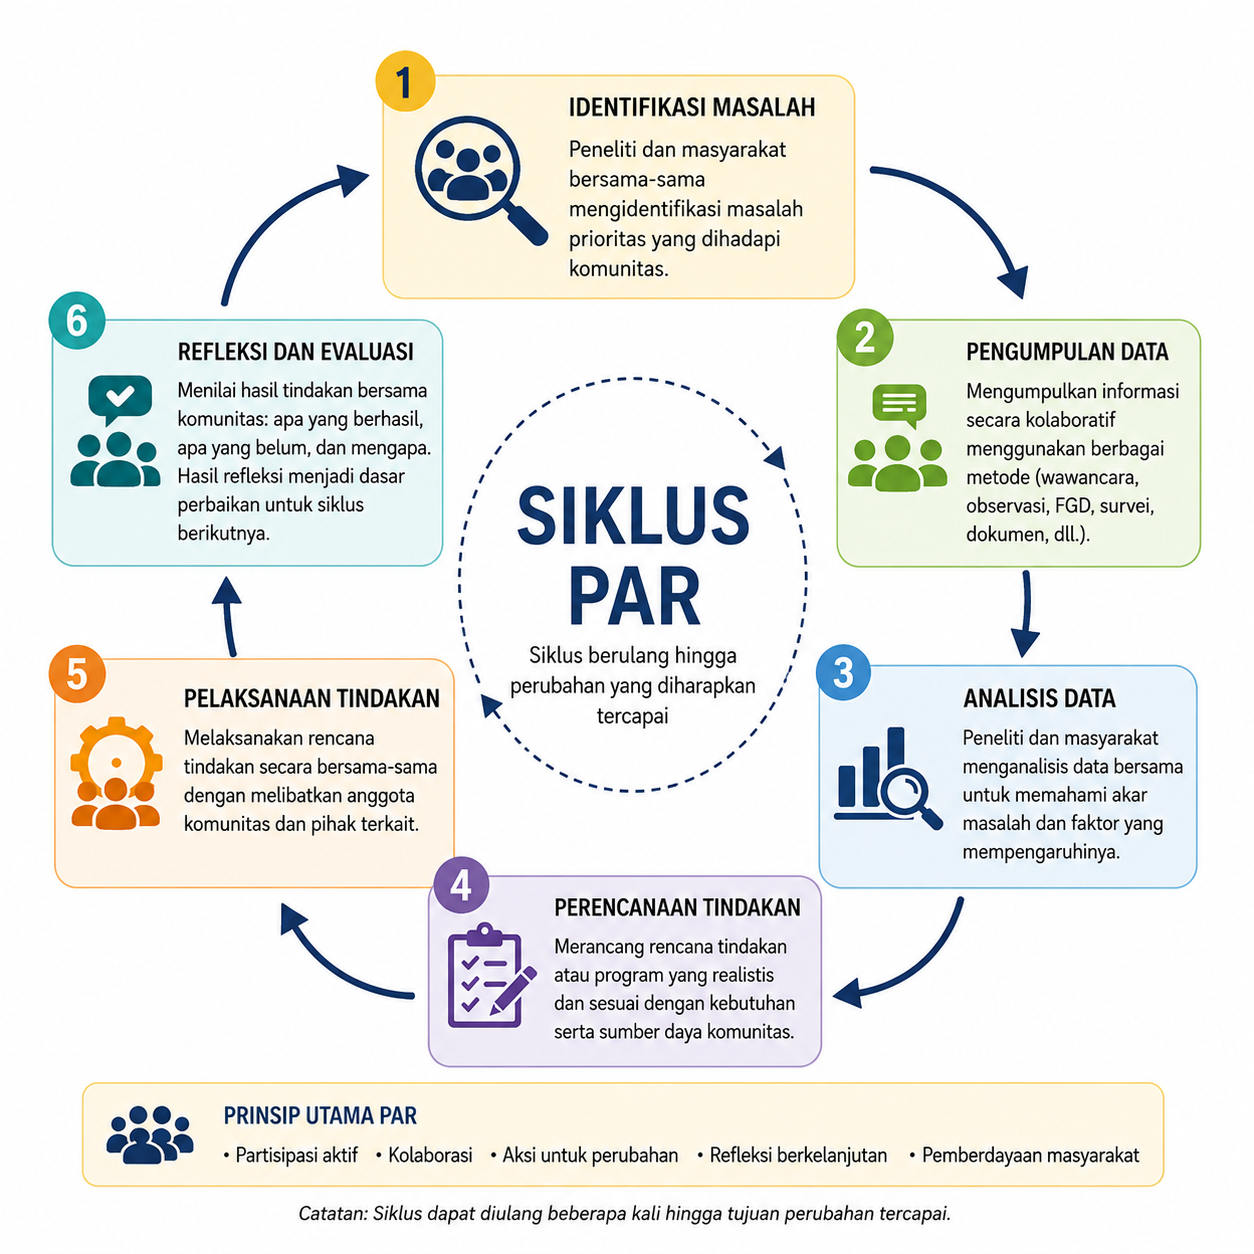
\includegraphics[keepaspectratio]{images/siklus.png}}
\caption{Siklus Pelaksanaan PAR}
\end{figure}

}

\caption{\label{fig-sikluspar}}

\end{figure}%

\subsection{Keunggulan PAR}\label{keunggulan-par}

\begin{enumerate}
\def\labelenumi{\arabic{enumi}.}
\tightlist
\item
  \textbf{Menghasilkan pengetahuan yang langsung dapat dimanfaatkan
  untuk memecahkan permasalahan} nyata yang dihadapi masyarakat.
\item
  \textbf{Meningkatkan partisipasi, kapasitas, dan rasa memiliki
  masyarakat terhadap program} atau solusi yang dikembangkan.
\item
  \textbf{Menjembatani kesenjangan antara teori dan praktik} karena
  hasil penelitian langsung diterapkan dalam bentuk tindakan.
\item
  \textbf{Mendorong kolaborasi antara peneliti, masyarakat, dan berbagai
  pemangku kepentingan} sehingga solusi yang dihasilkan lebih sesuai
  dengan kebutuhan komunitas.
\end{enumerate}

\subsection{Keterbatasan PAR}\label{keterbatasan-par}

\begin{enumerate}
\def\labelenumi{\arabic{enumi}.}
\tightlist
\item
  \textbf{Keberhasilan penelitian sangat bergantung pada tingkat
  partisipasi masyarakat} dan dukungan dari berbagai pemangku
  kepentingan.
\item
  Kolaborasi antara berbagai pihak \textbf{dapat menimbulkan perbedaan
  kepentingan maupun konflik} selama proses penelitian.
\item
  Penelitian \textbf{membutuhkan waktu yang relatif lama} karena
  dilakukan melalui beberapa siklus tindakan dan refleksi.
\item
  \textbf{Temuan penelitian sangat dipengaruhi oleh konteks lokal}
  sehingga hasilnya tidak dimaksudkan untuk digeneralisasikan secara
  statistik ke populasi yang lebih luas.
\end{enumerate}

\begin{tcolorbox}[enhanced jigsaw, colframe=quarto-callout-tip-color-frame, toptitle=1mm, breakable, leftrule=.75mm, arc=.35mm, toprule=.15mm, colback=white, colbacktitle=quarto-callout-tip-color!10!white, bottomtitle=1mm, bottomrule=.15mm, titlerule=0mm, title={Kapan menggunakan PAR?}, coltitle=black, left=2mm, opacitybacktitle=0.6, opacityback=0, rightrule=.15mm]

PAR tepat digunakan apabila tujuan penelitian adalah:

\begin{itemize}
\tightlist
\item
  menyelesaikan suatu permasalahan bersama komunitas;
\item
  mengembangkan atau mengevaluasi program berbasis komunitas;
\item
  melibatkan komunitas sebagai mitra dalam penelitian;
\item
  menghasilkan perubahan sosial sekaligus pengetahuan ilmiah.
\end{itemize}

Contoh pertanyaan penelitian:

\begin{itemize}
\tightlist
\item
  Bagaimana guru, siswa, dan orang tua dapat bekerja sama mengembangkan
  program promosi kesehatan mental di sekolah?
\item
  Bagaimana masyarakat Desa X dapat meningkatkan perilaku hidup bersih
  dan sehat melalui program berbasis komunitas?
\item
  Bagaimana mahasiswa dapat berkolaborasi merancang program pencegahan
  stres akademik di Fakultas Psikologi?
\item
  Bagaimana kader Posyandu bersama masyarakat meningkatkan partisipasi
  ibu balita dalam pemantauan tumbuh kembang anak?
\end{itemize}

\end{tcolorbox}

\section{Fenomenologi}\label{fenomenologi}

Fenomenologi merupakan desain penelitian kualitatif yang bertujuan
memahami makna dari pengalaman hidup (\emph{lived experiences})
seseorang terhadap suatu fenomena tertentu. Melalui penelitian
fenomenologi, peneliti berupaya menggambarkan bagaimana individu
mengalami, memaknai, dan memberikan arti terhadap pengalaman tersebut
berdasarkan sudut pandang orang yang mengalaminya secara langsung
(Creswell \& Poth, 2023; Smith dkk., 2022).

\subsection{Karakteristik
Fenomenologi}\label{karakteristik-fenomenologi}

Fokus utama fenomenologi adalah mengungkap \textbf{esensi
(\emph{essence})} dari suatu pengalaman, yaitu makna yang dianggap sama
atau esensial di antara individu yang mengalami fenomena tersebut
(Oranga \& Matere, 2023). Oleh karena itu, penelitian fenomenologi tidak
berfokus pada penjelasan hubungan sebab-akibat ataupun pengembangan
teori baru, melainkan pada pemahaman makna pengalaman yang dialami
partisipan. Pertanyaan penelitian dalam fenomenologi umumnya diawali
dengan \emph{``Bagaimana seseorang mengalami\ldots{}''} atau \emph{``Apa
makna pengalaman\ldots{}''}.

Penelitian fenomenologi melibatkan partisipan yang memiliki pengalaman
langsung terhadap fenomena yang diteliti dan biasanya dipilih secara
\emph{purposive}. Salah satu karakteristik penting dalam fenomenologi
adalah \textbf{\emph{bracketing}} atau \textbf{\emph{epoché}}, yaitu
upaya peneliti untuk menunda sementara asumsi, pengalaman, maupun
pengetahuan yang dimilikinya agar tidak memengaruhi proses memahami
pengalaman partisipan (Oluka, 2025).

\subsection{Metode Pengumpulan Data}\label{metode-pengumpulan-data-5}

Metode pengumpulan data utama dalam penelitian fenomenologi adalah
\textbf{wawancara mendalam}, baik yang bersifat tidak terstruktur maupun
semi-terstruktur. Wawancara dilakukan menggunakan pertanyaan terbuka
agar partisipan dapat menceritakan pengalaman mereka secara bebas sesuai
dengan sudut pandangnya sendiri.

Selain wawancara, peneliti dapat memanfaatkan FGD, observasi, catatan
refleksi, dokumen pribadi, maupun narasi tertulis apabila relevan dengan
tujuan penelitian. Berbagai sumber data tersebut digunakan untuk
memperoleh pemahaman yang lebih mendalam mengenai pengalaman hidup
partisipan.

\subsection{Keunggulan Fenomenologi}\label{keunggulan-fenomenologi}

\begin{enumerate}
\def\labelenumi{\alph{enumi}.}
\tightlist
\item
  \textbf{Menghasilkan pemahaman yang mendalam mengenai pengalaman hidup
  seseorang.} Pendekatan ini memungkinkan peneliti memahami makna
  subjektif yang diberikan partisipan terhadap suatu fenomena.
\item
  \textbf{Mengungkap aspek pengalaman yang sering kali sulit diukur
  secara kuantitatif}, seperti emosi, persepsi, keyakinan, dan kesadaran
  individu.
\item
  \textbf{Menghasilkan deskripsi yang kaya (\emph{thick description})}
  mengenai pengalaman partisipan sehingga memberikan gambaran yang lebih
  utuh tentang fenomena yang diteliti.
\item
  \textbf{Penerapan \emph{bracketing} membantu peneliti meminimalkan
  pengaruh asumsi pribadi} sehingga pengalaman partisipan menjadi fokus
  utama penelitian.
\end{enumerate}

\subsection{Keterbatasan Fenomenologi}\label{keterbatasan-fenomenologi}

\begin{enumerate}
\def\labelenumi{\alph{enumi}.}
\tightlist
\item
  \textbf{Pengumpulan dan analisis data membutuhkan waktu yang cukup
  lama}, terutama karena peneliti harus melakukan wawancara mendalam,
  mentranskripsikan data, serta mengidentifikasi tema-tema yang
  menggambarkan esensi pengalaman.
\item
  \textbf{Temuan penelitian tidak dimaksudkan untuk digeneralisasikan}
  karena melibatkan sedikit partisipan yang memiliki pengalaman yang
  sangat spesifik.
\item
  \textbf{Menjaga \emph{bracketing} bukanlah hal yang mudah.} Peneliti
  harus terus melakukan refleksi agar asumsi dan pengalaman pribadinya
  tidak memengaruhi interpretasi terhadap pengalaman partisipan.
\item
  \textbf{Penelitian sering kali membahas pengalaman yang sensitif atau
  traumatis}, sehingga peneliti perlu memperhatikan aspek etika,
  kesejahteraan psikologis partisipan, dan kemungkinan munculnya beban
  emosional selama penelitian.
\end{enumerate}

\begin{tcolorbox}[enhanced jigsaw, colframe=quarto-callout-tip-color-frame, toptitle=1mm, breakable, leftrule=.75mm, arc=.35mm, toprule=.15mm, colback=white, colbacktitle=quarto-callout-tip-color!10!white, bottomtitle=1mm, bottomrule=.15mm, titlerule=0mm, title={Kapan menggunakan fenomenologi?}, coltitle=black, left=2mm, opacitybacktitle=0.6, opacityback=0, rightrule=.15mm]

Fenomenologi tepat digunakan apabila tujuan penelitian adalah:

\begin{itemize}
\tightlist
\item
  memahami makna suatu pengalaman hidup;
\item
  menggali bagaimana seseorang mengalami suatu peristiwa;
\item
  mengidentifikasi esensi dari pengalaman yang dialami beberapa
  individu;
\item
  memahami pengalaman yang bersifat subjektif dan personal.
\end{itemize}

Contoh pertanyaan penelitian:

\begin{itemize}
\tightlist
\item
  Bagaimana pengalaman menjadi \emph{caregiver} pasien demensia?
\item
  Bagaimana pengalaman mahasiswa tunanetra mengikuti pembelajaran di
  perguruan tinggi?
\item
  Apa makna pengalaman menjadi penyintas gempa bumi bagi individu yang
  mengalaminya?
\item
  Bagaimana pengalaman perawat memberikan perawatan paliatif kepada
  pasien terminal?
\end{itemize}

\end{tcolorbox}

\section{\texorpdfstring{\emph{Grounded
Theory}}{Grounded Theory}}\label{grounded-theory}

\emph{Grounded theory} merupakan desain penelitian kualitatif yang
bertujuan mengembangkan teori substantif berdasarkan data yang diperoleh
di lapangan. Berbeda dengan penelitian yang berangkat dari teori untuk
diuji, \emph{grounded theory} justru membangun teori secara induktif
melalui proses pengumpulan dan analisis data yang berlangsung secara
berulang (iteratif) (Charmaz, 2025).

\subsection{\texorpdfstring{Karakteristik \emph{Grounded
Theory}}{Karakteristik Grounded Theory}}\label{karakteristik-grounded-theory}

Fokus utama \emph{grounded theory} adalah menjelaskan suatu
\textbf{proses}, \textbf{tindakan}, atau \textbf{interaksi sosial} yang
belum banyak dipahami melalui pengembangan teori yang berakar pada data
(\emph{grounded in data}) (Creswell \& Poth, 2023). Oleh karena itu,
\emph{grounded theory} tidak hanya bertujuan mendeskripsikan suatu
fenomena, tetapi juga menjelaskan bagaimana suatu proses berlangsung
serta faktor-faktor yang memengaruhinya.

Karakteristik utama \emph{grounded theory} meliputi analisis data yang
dilakukan secara bertahap melalui proses \emph{coding}, penggunaan
metode \emph{constant comparison} untuk membandingkan data secara
terus-menerus, penerapan \emph{theoretical sampling} dalam menentukan
partisipan berikutnya, serta penulisan \emph{memo} sebagai bagian dari
proses pengembangan teori. Selama penelitian berlangsung, pengumpulan
data dan analisis dilakukan secara bersamaan sehingga temuan awal dapat
mengarahkan proses pengumpulan data berikutnya (Charmaz, 2025; Creswell
\& Poth, 2023).

\subsection{Metode Pengumpulan Data}\label{metode-pengumpulan-data-6}

\emph{Grounded theory} dapat menggunakan berbagai metode pengumpulan
data, seperti wawancara mendalam, observasi, analisis dokumen, maupun
berbagai sumber data lain yang relevan dengan teori yang sedang
dikembangkan. Di antara berbagai metode tersebut, wawancara merupakan
teknik yang paling sering digunakan karena memungkinkan peneliti
menggali informasi secara mendalam mengenai proses atau interaksi yang
diteliti.

Pengumpulan data dilakukan secara bertahap dan berlangsung bersamaan
dengan proses analisis. Temuan awal digunakan sebagai dasar untuk
menentukan data atau partisipan berikutnya melalui \emph{theoretical
sampling}, sehingga proses pengumpulan data berakhir ketika kategori
yang dikembangkan telah mencapai \emph{theoretical saturation} atau
tidak lagi menghasilkan informasi baru yang bermakna (Tie dkk., 2019).

\subsection{\texorpdfstring{Keunggulan \emph{Grounded
Theory}}{Keunggulan Grounded Theory}}\label{keunggulan-grounded-theory}

\begin{enumerate}
\def\labelenumi{\arabic{enumi}.}
\tightlist
\item
  \textbf{Menghasilkan teori yang berakar pada data empiris.} Teori yang
  dikembangkan berasal dari temuan lapangan sehingga memiliki
  keterkaitan yang kuat dengan fenomena yang diteliti.
\item
  \textbf{Sangat sesuai untuk memahami proses atau interaksi sosial yang
  belum banyak dijelaskan oleh teori yang ada.} Pendekatan ini
  memungkinkan peneliti mengembangkan penjelasan baru mengenai suatu
  fenomena.
\item
  \textbf{Analisis dilakukan secara iteratif}, sehingga teori yang
  dikembangkan terus disempurnakan berdasarkan data yang diperoleh
  selama penelitian.
\item
  \textbf{Penerapan \emph{theoretical sampling} membantu peneliti
  memperoleh data yang paling relevan} untuk mengembangkan kategori dan
  teori yang sedang dibangun.
\end{enumerate}

\subsection{\texorpdfstring{Keterbatasan \emph{Grounded
Theory}}{Keterbatasan Grounded Theory}}\label{keterbatasan-grounded-theory}

\begin{enumerate}
\def\labelenumi{\arabic{enumi}.}
\tightlist
\item
  \textbf{Proses analisis data relatif kompleks.} Peneliti harus
  melakukan \emph{coding}, \emph{constant comparison}, penulisan
  \emph{memo}, dan pengembangan kategori secara sistematis sehingga
  pendekatan ini sering kali menjadi tantangan bagi peneliti pemula.
\item
  \textbf{Membutuhkan waktu yang cukup lama} karena pengumpulan data dan
  analisis dilakukan secara berulang hingga mencapai \emph{theoretical
  saturation}.
\item
  \textbf{Interpretasi teori tetap dipengaruhi oleh peneliti}, sehingga
  refleksivitas diperlukan untuk meminimalkan pengaruh asumsi pribadi
  selama proses pengembangan teori.
\item
  \textbf{Temuan penelitian sangat dipengaruhi oleh konteks sosial
  tempat penelitian dilakukan}, sehingga teori yang dihasilkan tidak
  selalu dapat diterapkan secara langsung pada konteks yang berbeda.
\end{enumerate}

\begin{tcolorbox}[enhanced jigsaw, colframe=quarto-callout-tip-color-frame, toptitle=1mm, breakable, leftrule=.75mm, arc=.35mm, toprule=.15mm, colback=white, colbacktitle=quarto-callout-tip-color!10!white, bottomtitle=1mm, bottomrule=.15mm, titlerule=0mm, title={Kapan menggunakan \emph{grounded theory}?}, coltitle=black, left=2mm, opacitybacktitle=0.6, opacityback=0, rightrule=.15mm]

\emph{Grounded theory} tepat digunakan apabila tujuan penelitian adalah:

\begin{itemize}
\tightlist
\item
  membangun teori baru mengenai suatu fenomena;
\item
  memahami bagaimana suatu proses atau interaksi berkembang;
\item
  menjelaskan tahapan atau mekanisme suatu perilaku;
\item
  meneliti fenomena yang masih sedikit memiliki landasan teori.
\end{itemize}

Contoh pertanyaan penelitian:

\begin{itemize}
\tightlist
\item
  Bagaimana proses terjadinya \emph{burnout} pada tenaga kesehatan di
  rumah sakit?
\item
  Bagaimana proses mahasiswa mengembangkan kecanduan gim daring hingga
  memengaruhi prestasi akademik?
\item
  Bagaimana proses terbentuknya resiliensi pada penyintas bencana alam?
\item
  Bagaimana proses pemulihan psikologis penyintas kekerasan dalam rumah
  tangga?
\end{itemize}

\end{tcolorbox}

Keenam desain penelitian kualitatif yang telah dibahas memiliki
karakteristik, tujuan, dan luaran yang berbeda sehingga pemilihannya
harus disesuaikan dengan tujuan penelitian, jenis pertanyaan penelitian,
serta fenomena yang ingin dipahami. Tidak ada satu desain yang lebih
baik daripada desain lainnya, karena masing-masing dikembangkan untuk
menjawab kebutuhan penelitian yang berbeda. Ringkasan perbandingan
karakteristik utama dari setiap desain penelitian kualitatif disajikan
pada Gambar~\ref{fig-desainkuali}, yang dapat digunakan sebagai panduan
dalam memilih desain penelitian yang paling sesuai.

\begin{figure}

\centering{

\begin{figure}
\centering
\pandocbounded{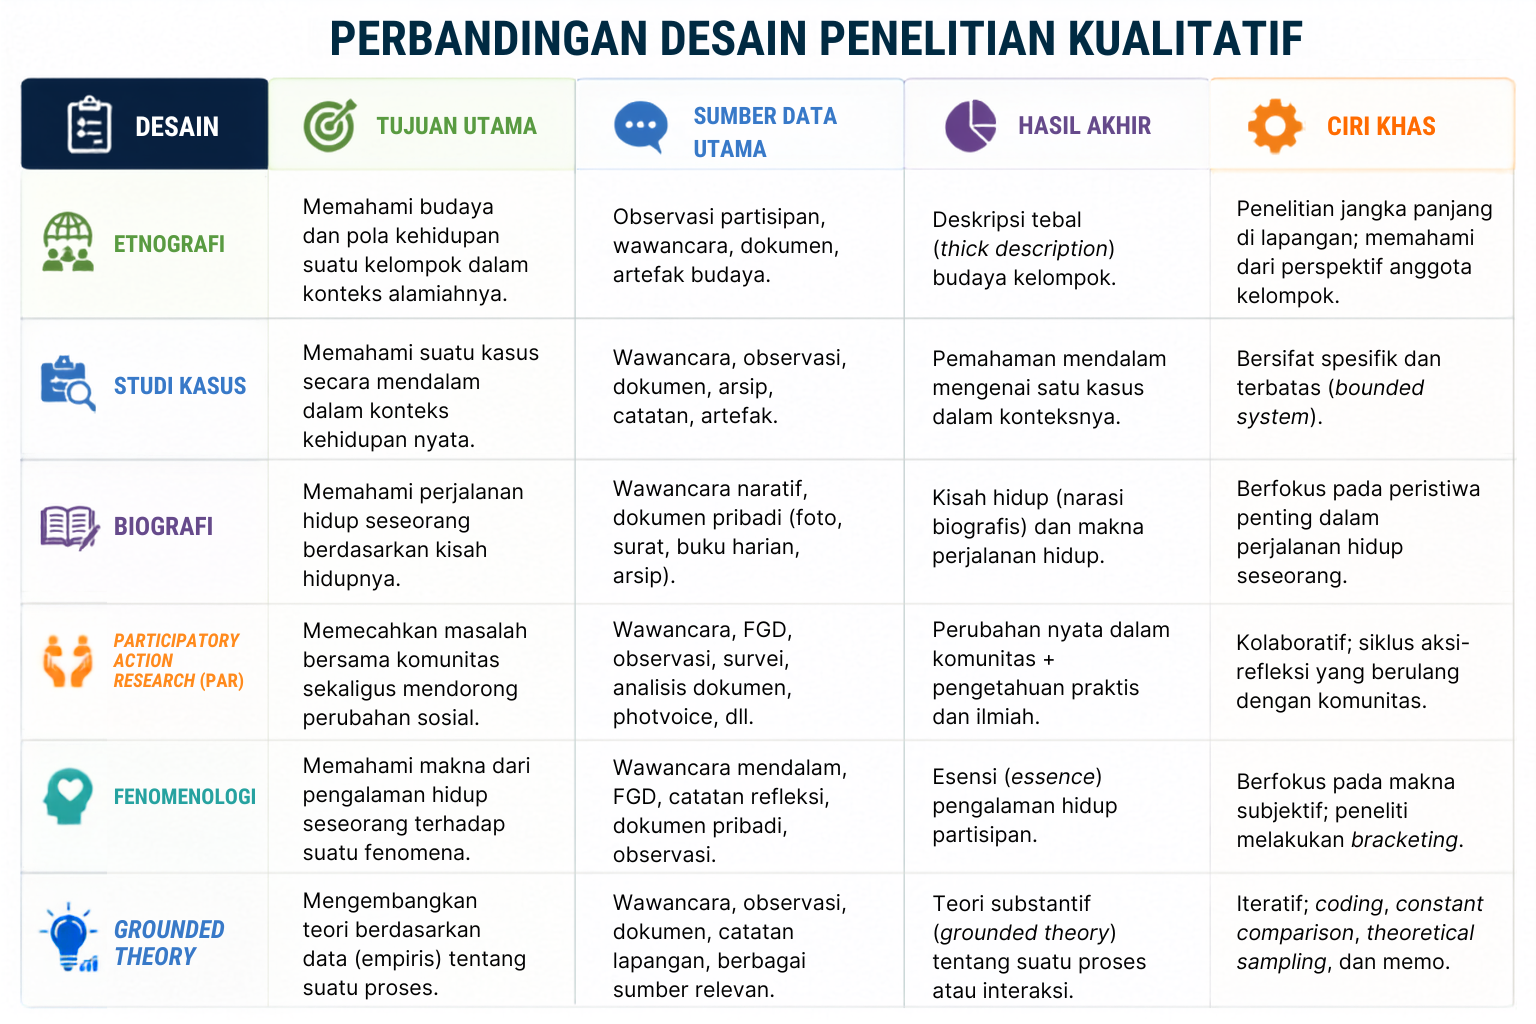
\includegraphics[keepaspectratio]{images/desain kualitatif.png}}
\caption{Perbandingan Desain Penelitian Kualitatif}
\end{figure}

}

\caption{\label{fig-desainkuali}}

\end{figure}%

Dari perbandingan tersebut terlihat bahwa perbedaan utama antar desain
penelitian kualitatif tidak terletak pada teknik pengumpulan datanya,
karena sebagian besar menggunakan wawancara dan observasi, melainkan
pada tujuan penelitian serta jenis pengetahuan yang ingin dihasilkan.
Oleh karena itu, pemilihan desain penelitian hendaknya didasarkan pada
pertanyaan penelitian dan fenomena yang ingin dipahami, bukan
semata-mata pada teknik pengumpulan data yang akan digunakan.

\begin{tcolorbox}[enhanced jigsaw, colframe=quarto-callout-tip-color-frame, toptitle=1mm, breakable, leftrule=.75mm, arc=.35mm, toprule=.15mm, colback=white, colbacktitle=quarto-callout-tip-color!10!white, bottomtitle=1mm, bottomrule=.15mm, titlerule=0mm, title=\textcolor{quarto-callout-tip-color}{\faLightbulb}\hspace{0.5em}{Rangkuman}, coltitle=black, left=2mm, opacitybacktitle=0.6, opacityback=0, rightrule=.15mm]

\begin{enumerate}
\def\labelenumi{\arabic{enumi}.}
\tightlist
\item
  Penelitian kualitatif memiliki berbagai desain yang dikembangkan untuk
  menjawab tujuan penelitian yang berbeda-beda, sehingga pemilihannya
  harus disesuaikan dengan pertanyaan penelitian dan fenomena yang ingin
  dipahami.
\item
  Etnografi digunakan untuk memahami budaya, nilai, norma, dan praktik
  sosial suatu kelompok melalui keterlibatan peneliti di lingkungan
  alami mereka.
\item
  Studi kasus berfokus pada pemahaman mendalam terhadap suatu kasus yang
  memiliki batasan yang jelas (\emph{bounded system}) dalam konteks
  kehidupan nyata.
\item
  Biografi bertujuan memahami perjalanan hidup seseorang melalui narasi
  pengalaman yang membentuk identitas dan kehidupannya.
\item
  \emph{Participatory Action Research} (PAR) melibatkan masyarakat
  sebagai mitra penelitian untuk menghasilkan pengetahuan sekaligus
  mendorong perubahan melalui siklus aksi dan refleksi.
\item
  Fenomenologi bertujuan memahami makna dari pengalaman hidup
  (\emph{lived experiences}) seseorang terhadap suatu fenomena dan
  mengidentifikasi esensi pengalaman tersebut.
\item
  \emph{Grounded theory} digunakan untuk mengembangkan teori substantif
  yang berakar pada data empiris melalui analisis yang berlangsung
  secara induktif dan iteratif.
\item
  Tidak ada desain penelitian kualitatif yang paling baik untuk semua
  situasi. Pemilihan desain harus mempertimbangkan tujuan penelitian,
  karakteristik fenomena, konteks penelitian, serta jenis pengetahuan
  yang ingin dihasilkan.
\end{enumerate}

\end{tcolorbox}

\begin{tcolorbox}[enhanced jigsaw, colframe=quarto-callout-important-color-frame, toptitle=1mm, breakable, leftrule=.75mm, arc=.35mm, toprule=.15mm, colback=white, colbacktitle=quarto-callout-important-color!10!white, bottomtitle=1mm, bottomrule=.15mm, titlerule=0mm, title=\textcolor{quarto-callout-important-color}{\faExclamation}\hspace{0.5em}{Refleksi \& Diskusi}, coltitle=black, left=2mm, opacitybacktitle=0.6, opacityback=0, rightrule=.15mm]

\begin{itemize}
\tightlist
\item
  Menurut Anda, apa perbedaan mendasar antara etnografi, studi kasus,
  biografi, \emph{participatory action research} (PAR), fenomenologi,
  dan \emph{grounded theory}? Jelaskan karakteristik yang paling
  membedakan masing-masing desain.
\item
  Pilih salah satu fenomena psikologis yang menarik bagi Anda, kemudian
  tentukan desain penelitian kualitatif yang paling sesuai untuk
  mengkajinya. Jelaskan alasan pemilihan desain tersebut.
\item
  Perhatikan sebuah artikel penelitian kualitatif yang Anda temukan dari
  jurnal ilmiah. Identifikasi desain penelitian yang digunakan, kemudian
  jelaskan apakah desain tersebut sudah sesuai dengan tujuan penelitian
  yang ingin dicapai.
\item
  Anda adalah seorang peneliti yang sedang meneliti fenomena ``Transisi
  Pembelajaran Berbasis Kecerdasan Buatan (AI) di Sekolah Menengah
  Daerah Terpencil''. Susunlah pertanyaan penelitian dari topik riset di
  atas di mana setiap pertanyaan mencerminkan karakteristik khas dan
  tujuan utama dari masing-masing desain riset yang telah dipelajari
  sebelumnya (etnografi,~ studi kasus, biografi,~ \emph{participatory
  action research,} fenomenologi, dan \emph{grounded theory}).
\end{itemize}

\end{tcolorbox}

\phantomsection\label{refs--17}
\begin{CSLReferences}{1}{0}
\bibitem[\citeproctext]{ref-Angrosino2008--17}
Angrosino, M. V. (2008). \emph{Doing Ethnographic and Observational
Research}. Sage Publications.

\bibitem[\citeproctext]{ref-Charmaz2025--17}
Charmaz, K. (2025). \emph{Constructing grounded theory} (3rd ed.). SAGE
Publications Ltd.

\bibitem[\citeproctext]{ref-Chevalier2019--17}
Chevalier, J. M., \& Buckles, D. (2019). \emph{Participatory action
research: Theory and methods for engaged inquiry} (2nd ed.). Routledge.

\bibitem[\citeproctext]{ref-Cornish2023--17}
Cornish, F., Breton, N., Moreno-Tabarez, U., Delgado, J., Rua, M.,
Aikins, A. de-Graft, \& Hodgetts, D. (2023). Participatory action
research. \emph{Nature Reviews Methods Primers}, \emph{3}, 34.
\url{https://doi.org/10.1038/s43586-023-00214-1}

\bibitem[\citeproctext]{ref-Creswell2023--17}
Creswell, J. W., \& Poth, C. N. (2023). \emph{Qualitative inquiry \&
research design: Choosing among five approaches} (5th ed.). SAGE
Publications, Inc.

\bibitem[\citeproctext]{ref-Fine2021--17}
Fine, M., Torre, M. E., Oswald, A. G., \& Avory, S. (2021). Critical
participatory action research: Methods and praxis for intersectional
knowledge production. \emph{Journal of Counseling Psychology},
\emph{68}, 344--356. \url{https://doi.org/10.1037/cou0000445}

\bibitem[\citeproctext]{ref-Hammersley2019--17}
Hammersley, M., \& Atkinson, P. (2019). \emph{Ethnography: Principles in
practice}. Routledge.

\bibitem[\citeproctext]{ref-Jacobs2018--17}
Jacobs, S. D. (2018). A History and Analysis of the Evolution of Action
and Participatory Action Research. \emph{The Canadian Journal of Action
Research}, \emph{19}, 34--52.
\url{https://doi.org/10.33524/cjar.v19i3.412}

\bibitem[\citeproctext]{ref-Oluka2025--17}
Oluka, A. (2025). Phenomenological Research Strategy: Descriptive and
Interpretive Approaches. \emph{F1000Research}, \emph{14}, 725.
\url{https://doi.org/10.12688/f1000research.166273.1}

\bibitem[\citeproctext]{ref-Oranga2023--17}
Oranga, J., \& Matere, A. (2023). Qualitative Research: Essence, Types
and Advantages. \emph{Open Access Library Journal}, \emph{10}, 1--9.
\url{https://doi.org/10.4236/oalib.1111001}

\bibitem[\citeproctext]{ref-Patton2014--17}
Patton, M. Q. (2014). \emph{Qualitative research \& evaluation methods:
Integrating theory and practice}. SAGE Publications, Inc.

\bibitem[\citeproctext]{ref-Priya2021--17}
Priya, A. (2021). Case Study Methodology of Qualitative Research: Key
Attributes and Navigating the Conundrums in Its Application.
\emph{Sociological Bulletin}, \emph{70}, 94--110.
\url{https://doi.org/10.1177/0038022920970318}

\bibitem[\citeproctext]{ref-Smith2022--17}
Smith, J. A., Flowers, P., \& Larkin, M. (2022). \emph{Interpretative
Phenomenological Analysis: Theory, Method and Research} (2nd ed.). SAGE
Publications Ltd.

\bibitem[\citeproctext]{ref-Stake1995--17}
Stake, R. E. (1995). \emph{The art of case study research}. Sage
Publications.

\bibitem[\citeproctext]{ref-Surez-Ortega2013--17}
Suárez-Ortega, M. (2013). Performance, Reflexivity, and Learning Through
Biographical-Narrative Research. \emph{Qualitative Inquiry}, \emph{19},
189--200. \url{https://doi.org/10.1177/1077800412466223}

\bibitem[\citeproctext]{ref-ChunTie2019--17}
Tie, Y. C., Birks, M., \& Francis, K. (2019). Grounded theory research:
A design framework for novice researchers. \emph{SAGE Open Medicine},
\emph{7}.
\url{https://doi.org/10.1177/2050312118822927;WGROUP:STRING:PUBLICATION}

\bibitem[\citeproctext]{ref-Willig2017--17}
Willig, C., \& Rogers, W. S. (2021). \emph{The SAGE Handbook of
Qualitative Research in Psychology}. SAGE Publications Ltd.
\url{https://doi.org/10.4135/9781526405555}

\bibitem[\citeproctext]{ref-Yin2018--17}
Yin, R. K., \& Campbell, D. T. (2018). \emph{Case study research and
applications: Design and methods}. SAGE Publications, Inc.

\end{CSLReferences}

\chapter{Populasi dan Sampling dalam Penelitian
Kualitatif}\label{populasi-dan-sampling-dalam-penelitian-kualitatif}

\begin{tcolorbox}[enhanced jigsaw, colframe=quarto-callout-note-color-frame, toptitle=1mm, breakable, leftrule=.75mm, arc=.35mm, toprule=.15mm, colback=white, colbacktitle=quarto-callout-note-color!10!white, bottomtitle=1mm, bottomrule=.15mm, titlerule=0mm, title=\textcolor{quarto-callout-note-color}{\faInfo}\hspace{0.5em}{Capaian Pembelajaran}, coltitle=black, left=2mm, opacitybacktitle=0.6, opacityback=0, rightrule=.15mm]

Setelah mempelajari bab ini, mahasiswa diharapkan mampu:

\begin{enumerate}
\def\labelenumi{\arabic{enumi}.}
\tightlist
\item
  Menjelaskan konsep populasi dan sampling dalam penelitian kualitatif.
\item
  Menentukan populasi, kriteria partisipan, dan strategi sampling yang
  sesuai dengan tujuan penelitian.
\item
  Menentukan jumlah partisipan berdasarkan kebutuhan penelitian dan
  prinsip saturasi data.
\item
  Menjelaskan berbagai strategi rekrutmen partisipan dalam penelitian
  kualitatif.
\item
  Menyusun prosedur sampling secara sistematis dalam proposal maupun
  laporan penelitian.
\end{enumerate}

\end{tcolorbox}

Dalam setiap penelitian, peneliti perlu menentukan siapa yang akan
menjadi sumber data penelitian. Keputusan tersebut mencakup penentuan
populasi, pemilihan partisipan, penetapan jumlah partisipan, serta cara
memperoleh partisipan yang sesuai dengan tujuan penelitian.

Berbeda dengan penelitian kuantitatif yang menekankan keterwakilan
sampel terhadap populasi, penelitian kualitatif lebih menekankan
pemilihan partisipan yang mampu memberikan informasi secara mendalam
mengenai fenomena yang diteliti. Oleh karena itu, proses \emph{sampling}
dalam penelitian kualitatif tidak hanya berkaitan dengan jumlah
partisipan, tetapi juga dengan pertimbangan mengenai siapa yang paling
tepat untuk diwawancarai atau diamati.

Bab ini membahas konsep populasi dan \emph{sampling} dalam penelitian
kualitatif, mulai dari penentuan populasi penelitian, pemilihan
partisipan, penentuan jumlah partisipan, strategi \emph{sampling},
proses rekrutmen partisipan, hingga cara melaporkan prosedur
\emph{sampling} dalam proposal maupun laporan penelitian.

\section{Menentukan Populasi
Penelitian}\label{menentukan-populasi-penelitian}

Penentuan populasi merupakan salah satu langkah awal yang penting dalam
penelitian kualitatif. Meskipun penelitian kualitatif tidak bertujuan
melakukan generalisasi statistik, peneliti tetap perlu menjelaskan
secara jelas siapa atau apa yang menjadi sasaran penelitiannya.
Kejelasan mengenai populasi akan membantu menentukan siapa yang layak
menjadi partisipan, batasan temuan penelitian, serta konteks di mana
hasil penelitian dapat dipahami.

Dalam literatur penelitian kualitatif, istilah \emph{population} atau
\emph{target population} masih digunakan. Namun, beberapa penulis,
seperti Robinson (2014), menggunakan istilah \emph{sample universe}
untuk menegaskan bahwa yang dimaksud bukan sekadar populasi dalam
pengertian statistik, melainkan keseluruhan individu atau kasus yang
secara logis dapat dipilih sebagai partisipan penelitian. Dengan kata
lain, \emph{sample universe} merupakan batas konseptual yang menunjukkan
siapa saja yang memenuhi syarat untuk menjadi sumber data penelitian.

\subsection{Konsep Populasi dalam Penelitian
Kualitatif}\label{konsep-populasi-dalam-penelitian-kualitatif}

Dalam penelitian kualitatif, populasi merujuk pada keseluruhan individu,
kelompok, organisasi, komunitas, atau kasus yang memiliki pengalaman
atau karakteristik yang relevan dengan fenomena yang ingin dipahami.
Patton (2014) menekankan bahwa penentuan populasi dalam penelitian
kualitatif harus selalu didasarkan pada tujuan penelitian (\emph{purpose
of inquiry}). Artinya, populasi tidak ditentukan oleh jumlah individu
yang tersedia, tetapi oleh siapa yang diperkirakan mampu memberikan
informasi yang paling kaya (\emph{information-rich cases}) mengenai
fenomena yang sedang dipelajari.

Robinson (2014) menyebut populasi tersebut sebagai \emph{sample
universe}, yaitu keseluruhan individu yang secara konseptual memenuhi
syarat untuk dijadikan partisipan penelitian. Penentuan \emph{sample
universe} dilakukan melalui penyusunan kriteria inklusi dan eksklusi
sehingga batas populasi menjadi jelas sejak awal penelitian.

Sebagai contoh, apabila penelitian bertujuan memahami pengalaman
mahasiswa yang mengalami \emph{academic burnout}, maka populasi
penelitian bukan seluruh mahasiswa, melainkan mahasiswa yang pernah
mengalami \emph{academic burnout}. Demikian pula, apabila penelitian
bertujuan mengeksplorasi pengalaman keluarga yang merawat anggota
keluarga dengan demensia, maka populasi penelitian adalah keluarga yang
memiliki pengalaman tersebut.

Dengan demikian, populasi dalam penelitian kualitatif tidak selalu
identik dengan kelompok yang besar. Yang lebih penting adalah kesesuaian
antara karakteristik populasi dengan fokus penelitian.

\subsection{Menentukan Populasi Berdasarkan Fokus
Penelitian}\label{menentukan-populasi-berdasarkan-fokus-penelitian}

Penentuan populasi dalam penelitian kualitatif selalu berangkat dari
pertanyaan penelitian (\emph{research question}). Oleh karena itu,
peneliti perlu terlebih dahulu mengidentifikasi fenomena yang ingin
dipahami sebelum menentukan siapa yang menjadi populasi penelitian.

Secara umum, populasi dalam penelitian kualitatif dapat ditentukan
melalui dua pendekatan:

\textbf{Pertama, berdasarkan fenomena yang dialami individu.} Dalam
pendekatan ini, populasi terdiri atas orang-orang yang memiliki
pengalaman tertentu sesuai dengan fokus penelitian. Contohnya,
penelitian mengenai pengalaman penyintas bencana alam menggunakan
populasi berupa individu yang pernah mengalami bencana tersebut.
Demikian pula penelitian mengenai pengalaman menjadi korban
\emph{cyberbullying} akan melibatkan individu yang pernah mengalami
perundungan di dunia maya.

\textbf{Kedua, berdasarkan kelompok atau konteks sosial tertentu.} Pada
pendekatan ini, populasi ditentukan berdasarkan keanggotaan seseorang
dalam suatu kelompok, organisasi, komunitas, atau lingkungan tertentu.
Sebagai contoh, penelitian mengenai budaya kerja pengemudi ojek daring
menjadikan seluruh pengemudi ojek daring sebagai populasi penelitian,
sedangkan penelitian mengenai adaptasi mahasiswa tahun pertama
menjadikan mahasiswa baru sebagai populasi penelitian.

Dalam praktiknya, kedua pendekatan tersebut sering digunakan secara
bersamaan. Misalnya, penelitian mengenai pengalaman \emph{burnout} pada
perawat ruang ICU memiliki populasi yang dibatasi oleh dua aspek
sekaligus, yaitu kelompok profesi (perawat ruang ICU) dan fenomena yang
dialami (\emph{burnout}).

Penentuan populasi yang spesifik akan membantu peneliti memperoleh data
yang lebih relevan serta memperjelas ruang lingkup temuan penelitian.

\subsection{Menentukan Kriteria Inklusi dan
Eksklusi}\label{menentukan-kriteria-inklusi-dan-eksklusi}

Setelah populasi penelitian ditetapkan, langkah berikutnya adalah
menentukan kriteria siapa saja yang dapat atau tidak dapat menjadi
partisipan penelitian. Robinson (2014) menyatakan bahwa penyusunan
kriteria inklusi (\emph{inclusion criteria}) dan kriteria eksklusi
(\emph{exclusion criteria}) merupakan langkah penting dalam membangun
\emph{sample universe} yang jelas.

Kriteria inklusi adalah karakteristik yang harus dimiliki seseorang agar
dapat diikutsertakan sebagai partisipan penelitian. Sebaliknya, kriteria
eksklusi adalah karakteristik yang menyebabkan seseorang tidak dapat
menjadi partisipan meskipun termasuk dalam populasi penelitian.

Sebagai contoh, penelitian mengenai pengalaman \emph{burnout} pada dosen
dapat menetapkan kriteria sebagai berikut.

\begin{quote}
\textbf{Kriteria inklusi}

\begin{itemize}
\tightlist
\item
  berstatus sebagai dosen aktif;
\item
  memiliki pengalaman \emph{burnout} dalam dua tahun terakhir;
\item
  bersedia mengikuti wawancara secara mendalam.
\end{itemize}

\textbf{Kriteria eksklusi}

\begin{itemize}
\tightlist
\item
  sedang menjalani cuti panjang;
\item
  memiliki gangguan kesehatan yang menghambat proses wawancara;
\item
  tidak bersedia direkam selama proses wawancara.
\end{itemize}
\end{quote}

Penyusunan kriteria inklusi dan eksklusi memberikan beberapa manfaat.
Pertama, membantu peneliti menjaga konsistensi dalam memilih partisipan.
Kedua, memastikan bahwa seluruh partisipan benar-benar relevan dengan
tujuan penelitian. Ketiga, meningkatkan transparansi penelitian karena
pembaca dapat memahami alasan mengapa seseorang dipilih atau tidak
dipilih sebagai partisipan.

Meskipun demikian, peneliti perlu berhati-hati agar kriteria yang
ditetapkan tidak terlalu sempit. Kriteria yang terlalu ketat dapat
menyulitkan proses rekrutmen partisipan dan membatasi variasi pengalaman
yang sebenarnya penting untuk dipahami. Sebaliknya, kriteria yang
terlalu longgar dapat menyebabkan data yang diperoleh menjadi kurang
terfokus. Oleh karena itu, penentuan kriteria inklusi dan eksklusi harus
selalu mempertimbangkan tujuan penelitian, pertanyaan penelitian, serta
pendekatan kualitatif yang digunakan.

\section{Memilih Partisipan
Penelitian}\label{memilih-partisipan-penelitian}

Setelah populasi penelitian ditetapkan, langkah berikutnya adalah
menentukan siapa yang akan dipilih sebagai partisipan penelitian. Pada
tahap inilah peneliti mulai menerapkan strategi \emph{sampling} yang
sesuai dengan tujuan penelitian. Pemilihan partisipan diarahkan untuk
memperoleh individu atau kelompok yang mampu memberikan informasi secara
mendalam mengenai fenomena yang diteliti.

Patton (2014) menyebut individu-individu tersebut sebagai
\emph{information-rich cases}, yaitu partisipan yang memiliki
pengalaman, pengetahuan, atau keterlibatan yang memadai sehingga mampu
memberikan informasi yang kaya dan bermakna bagi penelitian. Oleh karena
itu, pemilihan partisipan lebih berfokus pada individu atau kelompok
yang diperkirakan mampu memberikan informasi yang kaya, mendalam, dan
relevan dengan fenomena yang diteliti.

\begin{tcolorbox}[enhanced jigsaw, colframe=quarto-callout-note-color-frame, toptitle=1mm, breakable, leftrule=.75mm, arc=.35mm, toprule=.15mm, colback=white, colbacktitle=quarto-callout-note-color!10!white, bottomtitle=1mm, bottomrule=.15mm, titlerule=0mm, title=\textcolor{quarto-callout-note-color}{\faInfo}\hspace{0.5em}{Partisipan atau Responden?}, coltitle=black, left=2mm, opacitybacktitle=0.6, opacityback=0, rightrule=.15mm]

Dalam penelitian kualitatif, istilah \emph{partisipan} lebih sering
digunakan daripada \emph{responden} karena individu yang terlibat tidak
hanya memberikan jawaban atas pertanyaan penelitian, tetapi juga berbagi
pengalaman, pandangan, dan makna mengenai fenomena yang diteliti.

\end{tcolorbox}

\subsection{\texorpdfstring{\emph{Purposive Sampling} sebagai Strategi
Utama}{Purposive Sampling sebagai Strategi Utama}}\label{purposive-sampling-sebagai-strategi-utama}

Sebagian besar penelitian kualitatif menggunakan \emph{purposive
sampling} (\emph{purposeful sampling}), yaitu strategi memilih
partisipan secara sengaja berdasarkan pertimbangan bahwa mereka memiliki
pengalaman, pengetahuan, atau karakteristik yang relevan dengan tujuan
penelitian. Dalam praktiknya, \emph{purposive sampling} dapat diterapkan
melalui berbagai strategi, bergantung pada tujuan penelitian,
karakteristik fenomena yang dikaji, serta jenis informasi yang ingin
diperoleh. Beberapa strategi yang paling umum digunakan dijelaskan pada
bagian berikut (Creswell \& Creswell, 2023; Patton, 2014; Robinson,
2014).

\begin{enumerate}
\def\labelenumi{\arabic{enumi}.}
\item
  \textbf{\emph{Criterion Sampling}}

  \emph{Criterion sampling} merupakan strategi memilih partisipan
  berdasarkan seperangkat kriteria yang telah ditentukan sebelumnya.
  Seluruh partisipan yang terlibat harus memenuhi kriteria tersebut
  sehingga benar-benar memiliki pengalaman yang relevan dengan fenomena
  yang sedang diteliti. Strategi ini banyak digunakan dalam penelitian
  fenomenologi karena seluruh partisipan diharapkan memiliki pengalaman
  yang sama terhadap fenomena yang dikaji.

  Sebagai contoh, penelitian mengenai pengalaman \emph{academic burnout}
  dapat menetapkan bahwa partisipan harus merupakan mahasiswa aktif yang
  sedang menyusun skripsi dan pernah mengalami \emph{burnout} dalam satu
  tahun terakhir. Dengan demikian, mahasiswa yang tidak memenuhi
  kriteria tersebut tidak diikutsertakan dalam penelitian.
\item
  \textbf{\emph{Homogeneous Sampling}}

  \emph{Homogeneous sampling} memilih partisipan yang memiliki
  karakteristik yang relatif seragam. Tujuan utamanya adalah memperoleh
  pemahaman yang mendalam mengenai pengalaman kelompok tertentu tanpa
  dipengaruhi oleh terlalu banyak variasi karakteristik. Strategi ini
  sering digunakan dalam penelitian fenomenologi, \emph{interpretative
  phenomenological analysis} (IPA), maupun penelitian yang berfokus pada
  pengalaman kelompok tertentu.

  Sebagai contoh, penelitian mengenai pengalaman menjadi orang tua
  tunggal dapat melibatkan perempuan berusia 30--45 tahun yang
  membesarkan anak tanpa pasangan. Kesamaan karakteristik tersebut
  membantu peneliti mengidentifikasi pengalaman yang menjadi ciri khas
  kelompok tersebut.
\item
  \textbf{\emph{Maximum Variation Sampling}}

  Berbeda dengan \emph{homogeneous sampling}, \emph{maximum variation
  sampling} bertujuan memperoleh keragaman pengalaman yang seluas
  mungkin. Peneliti secara sengaja memilih partisipan yang memiliki
  karakteristik yang berbeda sehingga dapat mengeksplorasi bagaimana
  suatu fenomena dialami dalam berbagai konteks.

  Sebagai contoh, penelitian mengenai pengalaman menggunakan kecerdasan
  artifisial dalam pembelajaran dapat melibatkan mahasiswa dari berbagai
  program studi, semester, jenis perguruan tinggi, dan daerah asal.
  Melalui variasi tersebut, peneliti dapat mengidentifikasi tema-tema
  yang muncul secara konsisten meskipun partisipan berasal dari latar
  belakang yang berbeda.
\item
  \textbf{\emph{Typical Case Sampling}}

  \emph{Typical case sampling} digunakan apabila peneliti ingin memahami
  kondisi yang dianggap umum atau lazim terjadi pada suatu populasi.
  Oleh karena itu, partisipan dipilih karena dianggap mewakili
  karakteristik yang paling sering ditemukan, bukan karena memiliki
  pengalaman yang unik atau ekstrem.

  Sebagai contoh, penelitian mengenai pengalaman belajar mahasiswa tahun
  pertama dapat memilih mahasiswa dengan prestasi akademik, latar
  belakang sosial, dan aktivitas yang mencerminkan kondisi mayoritas
  mahasiswa pada program studi tersebut.
\item
  \textbf{\emph{Extreme}} \textbf{atau \emph{Deviant Case Sampling}}

  Pada strategi ini, peneliti secara sengaja memilih partisipan yang
  memiliki karakteristik atau pengalaman yang sangat berbeda dari
  kondisi umum. Kasus-kasus tersebut sering kali memberikan wawasan baru
  mengenai faktor-faktor yang memengaruhi suatu fenomena.

  Misalnya, penelitian mengenai resiliensi dapat memilih individu yang
  mampu bangkit kembali setelah mengalami berbagai peristiwa traumatis
  yang berat. Contoh lainnya adalah penelitian mengenai prestasi
  akademik yang melibatkan mahasiswa dengan capaian akademik yang sangat
  tinggi atau sangat rendah.
\item
  \textbf{\emph{Intensity Sampling}}

  \emph{Intensity sampling} memilih partisipan yang mengalami fenomena
  secara kuat, tetapi masih berada dalam rentang yang dianggap normal.
  Strategi ini berbeda dengan \emph{extreme case sampling} karena
  partisipan tidak dipilih berdasarkan kondisi yang sangat menyimpang,
  melainkan karena memiliki pengalaman yang cukup intens sehingga mampu
  memberikan informasi yang kaya.

  Sebagai contoh, penelitian mengenai stres kerja dapat memilih tenaga
  kesehatan yang memiliki tingkat stres tinggi, tetapi belum mengalami
  gangguan psikologis yang berat.
\item
  \textbf{\emph{Critical Case Sampling}}

  \emph{Critical case sampling} digunakan apabila peneliti ingin
  mempelajari kasus yang dipandang sangat penting atau strategis. Kasus
  tersebut dipilih karena diyakini mampu memberikan informasi yang
  memiliki implikasi luas terhadap pemahaman suatu fenomena.

  Sebagai contoh, penelitian mengenai implementasi kurikulum baru dapat
  memilih sekolah yang menjadi proyek percontohan nasional. Pengalaman
  sekolah tersebut diperkirakan dapat memberikan pelajaran penting bagi
  penerapan kebijakan pada sekolah lain.
\item
  \textbf{\emph{Theoretical Sampling}}

  Berbeda dengan strategi sebelumnya, \emph{theoretical sampling}
  merupakan strategi yang secara khusus digunakan dalam pendekatan
  \emph{grounded theory}. Pada strategi ini, pemilihan partisipan tidak
  ditetapkan sepenuhnya sejak awal penelitian, tetapi berkembang
  mengikuti proses analisis data. Karena bertujuan membangun teori,
  \emph{theoretical sampling} merupakan ciri khas penelitian
  \emph{grounded theory} dan umumnya tidak digunakan pada pendekatan
  kualitatif lainnya.

  Peneliti menentukan siapa yang perlu diwawancarai berikutnya
  berdasarkan kategori atau konsep yang mulai muncul selama analisis
  berlangsung. Proses tersebut dilakukan secara berulang hingga kategori
  yang dikembangkan telah mencapai saturasi teoritis (\emph{theoretical
  saturation}).
\end{enumerate}

Berbagai strategi \emph{purposive sampling} memiliki tujuan dan konteks
penggunaan yang berbeda. Pemilihan strategi yang tepat perlu disesuaikan
dengan pertanyaan penelitian, karakteristik fenomena yang dikaji, serta
jenis informasi yang ingin diperoleh. Ringkasan karakteristik
masing-masing strategi disajikan pada Tabel~\ref{tbl-samplingkuali}.

\begin{longtable}[]{@{}
  >{\raggedright\arraybackslash}p{(\linewidth - 4\tabcolsep) * \real{0.2917}}
  >{\raggedright\arraybackslash}p{(\linewidth - 4\tabcolsep) * \real{0.4444}}
  >{\raggedright\arraybackslash}p{(\linewidth - 4\tabcolsep) * \real{0.2639}}@{}}
\caption{Perbandingan tujuan setiap metode sampling metode
kualitatif}\label{tbl-samplingkuali}\tabularnewline
\toprule\noalign{}
\endfirsthead
\endhead
\bottomrule\noalign{}
\endlastfoot
\textbf{Strategi} & \textbf{Tujuan} & \textbf{Contoh Penelitian} \\
\emph{Criterion} & Memilih partisipan yang memenuhi kriteria tertentu &
Pengalaman penyintas stroke \\
\emph{Homogeneous} & Mendalami pengalaman kelompok yang seragam &
Pengalaman mahasiswa tingkat akhir menyusun skripsi \\
\emph{Maximum variation} & Mengeksplorasi keragaman pengalaman &
Penggunaan AI oleh mahasiswa dari berbagai program studi \\
\emph{Typical case} & Menggambarkan kondisi umum & Pengalaman belajar
mahasiswa tahun pertama \\
\emph{Extreme/deviant} & Mengkaji kasus tidak biasa & Resiliensi pada
penyintas bencana dengan pemulihan luar biasa \\
\emph{Intensity} & Mengkaji fenomena yang kuat tetapi tidak ekstrem &
Stres kerja pada tenaga kesehatan \\
\emph{Critical case} & Mempelajari kasus yang strategis & Implementasi
kurikulum di sekolah percontohan \\
\emph{Theoretical} & Mengembangkan teori & Penelitian \emph{grounded
theory} \\
\end{longtable}

\subsection{\texorpdfstring{\emph{Snowball
Sampling}}{Snowball Sampling}}\label{snowball-sampling}

Selain \emph{purposive sampling}, strategi lain yang cukup sering
digunakan dalam penelitian kualitatif adalah \emph{snowball sampling}.
Pada strategi ini, peneliti memperoleh partisipan baru melalui
rekomendasi dari partisipan yang telah diwawancarai sebelumnya. Dengan
kata lain, setiap partisipan membantu peneliti menemukan partisipan lain
yang memenuhi kriteria penelitian sehingga jumlah partisipan bertambah
secara bertahap seperti bola salju yang menggelinding.

\emph{Snowball sampling} umumnya digunakan ketika populasi penelitian
sulit diidentifikasi atau tidak memiliki daftar anggota yang jelas.
Kondisi ini banyak dijumpai pada penelitian yang melibatkan kelompok
tersembunyi (\emph{hidden populations}), seperti penyintas kekerasan
seksual, pengguna narkotika, individu yang hidup dengan HIV/AIDS, atau
kelompok minoritas tertentu. Dalam situasi tersebut, rekomendasi dari
partisipan sebelumnya sering menjadi cara yang paling efektif untuk
memperoleh akses kepada calon partisipan berikutnya (Creswell \&
Creswell, 2023; Patton, 2014).

Meskipun demikian, \emph{snowball sampling} memiliki beberapa
keterbatasan. Karena partisipan direkrut melalui jaringan sosial yang
saling berkaitan, terdapat kemungkinan bahwa karakteristik partisipan
menjadi kurang beragam sehingga data yang diperoleh cenderung berasal
dari kelompok yang memiliki pengalaman atau pandangan yang serupa. Oleh
karena itu, peneliti perlu mempertimbangkan potensi bias tersebut ketika
menafsirkan hasil penelitian.

Dalam banyak buku metodologi penelitian, \emph{snowball sampling}
diklasifikasikan sebagai salah satu teknik \emph{non-probability
sampling} (Bordens \& Abbott, 2018; Morling, 2024; Neuman, 2014). Namun,
beberapa penulis memandang bahwa \emph{snowball sampling} tidak hanya
merupakan strategi pemilihan partisipan, tetapi juga merupakan cara
untuk memperoleh akses kepada partisipan yang memenuhi kriteria
penelitian. Oleh karena itu, pembahasan mengenai penerapan
\emph{snowball sampling} dalam proses rekrutmen partisipan akan
dijelaskan lebih lanjut pada Bab~\ref{sec-snowball}.

\section{Menentukan Jumlah
Partisipan}\label{menentukan-jumlah-partisipan}

Salah satu pertanyaan yang paling sering diajukan oleh mahasiswa ketika
merancang penelitian kualitatif adalah, \emph{``Berapa jumlah partisipan
yang harus saya libatkan?''} Berbeda dengan penelitian kuantitatif yang
sering menggunakan rumus atau perhitungan statistik untuk menentukan
ukuran sampel, penelitian kualitatif tidak memiliki aturan baku mengenai
jumlah partisipan yang harus dilibatkan.

Dalam penelitian kualitatif, jumlah partisipan ditentukan berdasarkan
kemampuan data yang diperoleh untuk menjawab pertanyaan penelitian
secara mendalam. Oleh karena itu, keputusan mengenai jumlah partisipan
tidak hanya mempertimbangkan banyaknya individu yang diwawancarai,
tetapi juga kualitas informasi yang diperoleh, kompleksitas fenomena
yang diteliti, serta tujuan penelitian (Creswell \& Creswell, 2023;
Patton, 2014).

\subsection{Faktor yang Memengaruhi Jumlah
Partisipan}\label{faktor-yang-memengaruhi-jumlah-partisipan}

Tidak ada jumlah partisipan yang dapat diterapkan pada semua penelitian
kualitatif. Penentuan jumlah partisipan dipengaruhi oleh berbagai
faktor, antara lain sebagai berikut (Robinson, 2014; Strauss \& Corbin,
1998):

\begin{itemize}
\tightlist
\item
  \textbf{Tujuan penelitian.} Penelitian yang bertujuan mengeksplorasi
  pengalaman secara mendalam umumnya membutuhkan jumlah partisipan yang
  lebih sedikit dibandingkan penelitian yang ingin memperoleh variasi
  pengalaman dari berbagai kelompok.
\item
  \textbf{Pendekatan penelitian.} Setiap pendekatan kualitatif memiliki
  karakteristik yang berbeda. Misalnya, penelitian biografi umumnya
  hanya berfokus pada satu individu, sedangkan etnografi dapat
  melibatkan banyak informan dari suatu komunitas. Pada \emph{grounded
  theory}, jumlah partisipan berkembang mengikuti proses pengembangan
  teori.
\item
  \textbf{Keragaman partisipan.} Penelitian yang melibatkan partisipan
  dengan latar belakang yang sangat beragam biasanya memerlukan lebih
  banyak partisipan dibandingkan penelitian yang menggunakan kelompok
  yang relatif homogen.
\item
  \textbf{Kompleksitas fenomena.} Fenomena yang sederhana mungkin dapat
  dipahami melalui sedikit partisipan, sedangkan fenomena yang kompleks
  sering kali memerlukan eksplorasi dari berbagai perspektif.
\item
  \textbf{Kualitas data.} Partisipan yang memiliki pengalaman yang kaya
  dan mampu menjelaskan fenomena secara rinci sering kali menghasilkan
  data yang lebih bermakna daripada jumlah partisipan yang banyak tetapi
  memberikan informasi yang terbatas.
\end{itemize}

Dengan demikian, penentuan jumlah partisipan tidak dapat dilepaskan dari
konteks penelitian yang dilakukan.

\subsection{Konsep Saturasi Data}\label{konsep-saturasi-data}

Dalam penelitian kualitatif, proses pengambilan partisipan umumnya
dihentikan ketika peneliti mencapai \textbf{saturasi data} (\emph{data
saturation}). Saturasi data adalah kondisi ketika proses pengumpulan
data tidak lagi menghasilkan informasi, tema, atau kategori baru yang
relevan dengan tujuan penelitian (Guest dkk., 2006).

Sebagai ilustrasi, seorang peneliti melakukan wawancara mengenai
pengalaman mahasiswa yang mengalami \emph{academic burnout}. Pada
beberapa wawancara pertama, peneliti menemukan berbagai tema baru,
seperti tekanan akademik, tuntutan keluarga, kesulitan mengatur waktu,
dan kelelahan emosional. Namun, setelah melakukan sejumlah wawancara
berikutnya, tema-tema yang muncul mulai berulang dan tidak lagi
memberikan informasi baru. Pada kondisi inilah peneliti dapat
mempertimbangkan bahwa saturasi data telah tercapai.

Perlu dipahami bahwa saturasi bukan berarti seluruh partisipan
memberikan jawaban yang sama. Sebaliknya, saturasi menunjukkan bahwa
informasi yang diperoleh telah cukup untuk menjelaskan fenomena yang
sedang diteliti sehingga pengumpulan data tambahan diperkirakan tidak
lagi memberikan kontribusi yang bermakna terhadap analisis.

Konsep saturasi data terutama banyak digunakan pada penelitian
fenomenologi, studi kasus, dan \emph{grounded theory}. Pada
\emph{grounded theory}, istilah yang sering digunakan adalah
\textbf{saturasi teoritis} (\emph{theoretical saturation}), yaitu
kondisi ketika pengumpulan data tidak lagi menghasilkan kategori atau
hubungan konseptual baru yang diperlukan untuk membangun teori (Charmaz,
2014; Strauss \& Corbin, 1998).

Kecepatan tercapainya saturasi data dipengaruhi oleh berbagai faktor,
seperti tingkat homogenitas partisipan, kompleksitas fenomena yang
diteliti, kualitas wawancara, serta tujuan penelitian. Penelitian yang
melibatkan partisipan dengan karakteristik relatif homogen sering kali
mencapai saturasi lebih cepat dibandingkan penelitian yang melibatkan
partisipan dengan latar belakang yang sangat beragam (Hennink dkk.,
2017).

\subsection{Apakah Penelitian Kualitatif Dapat Menggunakan Satu
Partisipan?}\label{apakah-penelitian-kualitatif-dapat-menggunakan-satu-partisipan}

Salah satu anggapan yang masih sering dijumpai adalah bahwa penelitian
yang baik harus melibatkan banyak partisipan. Anggapan tersebut tidak
selalu berlaku dalam penelitian kualitatif.

Pada pendekatan tertentu, penggunaan satu partisipan atau satu kasus
justru dapat dibenarkan apabila kasus tersebut memiliki nilai ilmiah
yang tinggi dan mampu memberikan pemahaman yang mendalam mengenai
fenomena yang diteliti. Sebagai contoh, penelitian biografi secara
khusus berfokus pada kehidupan satu individu, sedangkan studi kasus
dapat menelaah secara mendalam satu organisasi, satu keluarga, satu
sekolah, atau satu peristiwa tertentu (Yin \& Campbell, 2018).

Demikian pula, penelitian \emph{interpretative phenomenological
analysis} (IPA) sering menggunakan jumlah partisipan yang relatif
sedikit agar setiap pengalaman dapat dianalisis secara mendalam (Smith
dkk., 2021). Oleh karena itu, penggunaan satu partisipan tidak dapat
dinilai hanya berdasarkan jumlahnya, tetapi harus dipahami dalam konteks
pendekatan penelitian dan tujuan analisis yang dilakukan.

\section{Merekrut Partisipan
Penelitian}\label{merekrut-partisipan-penelitian}

Setelah menentukan strategi \emph{sampling} dan jumlah partisipan,
langkah berikutnya adalah merekrut partisipan yang sesuai dengan
kriteria penelitian. Tujuan utama proses rekrutmen adalah memperoleh
partisipan yang benar-benar memenuhi karakteristik yang telah ditetapkan
sehingga mampu memberikan informasi yang relevan dengan fokus
penelitian.

Cara merekrut partisipan bergantung pada karakteristik populasi,
kemudahan akses, serta konteks penelitian. Pada beberapa penelitian,
partisipan dapat dihubungi secara langsung, sedangkan pada penelitian
lain peneliti perlu bekerja sama dengan pihak tertentu atau menggunakan
jaringan partisipan yang telah direkrut sebelumnya.

\subsection{Rekrutmen Secara Langsung}\label{rekrutmen-secara-langsung}

Apabila populasi penelitian mudah diidentifikasi, peneliti dapat
menghubungi calon partisipan secara langsung, misalnya melalui surat
elektronik, telepon, media sosial, atau komunikasi tatap muka. Pada
tahap awal, peneliti perlu menjelaskan tujuan penelitian, bentuk
partisipasi yang diharapkan, serta hak calon partisipan untuk menerima
atau menolak keikutsertaan dalam penelitian.

\subsection{\texorpdfstring{Rekrutmen Melalui
\emph{Gatekeeper}}{Rekrutmen Melalui Gatekeeper}}\label{rekrutmen-melalui-gatekeeper}

Pada beberapa penelitian, akses terhadap partisipan memerlukan bantuan
pihak yang memiliki kewenangan atau hubungan dengan kelompok sasaran.
Pihak tersebut dikenal sebagai \emph{gatekeeper}, misalnya kepala
sekolah, pimpinan organisasi, ketua komunitas, atau tenaga kesehatan.

Peran \emph{gatekeeper} adalah membantu peneliti memperoleh akses kepada
calon partisipan. Namun demikian, keputusan untuk berpartisipasi tetap
harus berasal dari masing-masing individu tanpa adanya unsur paksaan.

\subsection{\texorpdfstring{\emph{Snowball
Sampling}}{Snowball Sampling}}\label{sec-snowball}

Apabila populasi penelitian sulit dijangkau atau tidak memiliki daftar
anggota yang jelas, peneliti dapat menggunakan \emph{snowball sampling}.
Pada teknik ini, peneliti meminta partisipan yang telah diwawancarai
untuk merekomendasikan individu lain yang memenuhi kriteria penelitian.

\emph{Snowball sampling} banyak digunakan pada penelitian yang
melibatkan populasi tersembunyi (\emph{hidden populations}), seperti
penyintas kekerasan, pengguna narkotika, atau kelompok minoritas
tertentu. Meskipun efektif untuk menemukan partisipan, teknik ini
berpotensi menghasilkan partisipan yang berasal dari jaringan sosial
yang sama sehingga peneliti perlu mempertimbangkan kemungkinan bias yang
muncul.

\subsection{Tantangan dalam Rekrutmen
Partisipan}\label{tantangan-dalam-rekrutmen-partisipan}

Proses rekrutmen tidak selalu berjalan sesuai rencana. Peneliti dapat
menghadapi berbagai kendala, seperti kesulitan menemukan partisipan yang
memenuhi kriteria, rendahnya kesediaan calon partisipan, atau
terbatasnya akses terhadap kelompok sasaran. Oleh karena itu, peneliti
perlu menyiapkan strategi rekrutmen yang fleksibel dan mendokumentasikan
proses rekrutmen sebagai bagian dari transparansi metodologi penelitian.

\section{\texorpdfstring{Menuliskan Prosedur \emph{Sampling} dalam
Proposal dan Laporan
Penelitian}{Menuliskan Prosedur Sampling dalam Proposal dan Laporan Penelitian}}\label{menuliskan-prosedur-sampling-dalam-proposal-dan-laporan-penelitian}

Selain melaksanakan proses \emph{sampling} dengan benar, peneliti juga
perlu menjelaskan prosedur tersebut secara jelas dalam proposal maupun
laporan penelitian. Uraian mengenai \emph{sampling} membantu pembaca
memahami siapa yang menjadi partisipan penelitian, bagaimana mereka
dipilih, serta alasan penggunaan strategi \emph{sampling} tertentu.
Penjelasan yang lengkap juga meningkatkan transparansi dan kredibilitas
penelitian.

Secara umum, bagian metode penelitian perlu memuat beberapa informasi
berikut.

\begin{enumerate}
\def\labelenumi{\arabic{enumi}.}
\item
  \textbf{Populasi Penelitian}

  Peneliti perlu menjelaskan siapa yang menjadi populasi atau kelompok
  sasaran penelitian. Penjelasan tersebut sebaiknya disesuaikan dengan
  fokus penelitian sehingga pembaca memahami konteks penelitian yang
  dilakukan.

  \textbf{Contoh:}

  \begin{quote}
  Populasi penelitian ini adalah mahasiswa program sarjana yang sedang
  menyusun skripsi pada sebuah perguruan tinggi di Jakarta.
  \end{quote}
\item
  \textbf{Kriteria Partisipan}

  Setelah menjelaskan populasi penelitian, peneliti perlu menguraikan
  kriteria inklusi dan, apabila diperlukan, kriteria eksklusi yang
  digunakan dalam memilih partisipan.

  \textbf{Contoh:}

  \begin{quote}
  Partisipan penelitian dipilih dengan kriteria sebagai berikut: (1)
  berstatus sebagai mahasiswa aktif, (2) sedang menyusun skripsi, dan
  (3) pernah mengalami \emph{academic burnout}.
  \end{quote}

  Penjelasan mengenai kriteria partisipan menunjukkan bahwa pemilihan
  partisipan dilakukan secara sistematis dan sesuai dengan tujuan
  penelitian.
\item
  \textbf{Strategi \emph{Sampling}}

  Peneliti perlu menjelaskan strategi \emph{sampling} yang digunakan
  beserta alasan pemilihannya.

  \textbf{Contoh:}

  \begin{quote}
  Penelitian ini menggunakan \emph{purposive sampling} karena bertujuan
  memperoleh partisipan yang memiliki pengalaman secara langsung
  terhadap fenomena \emph{academic burnout}.
  \end{quote}

  Apabila menggunakan \emph{snowball sampling}, peneliti juga perlu
  menjelaskan alasan penggunaan strategi tersebut, misalnya karena
  populasi penelitian sulit dijangkau atau tidak memiliki daftar anggota
  yang jelas.
\item
  \textbf{Jumlah Partisipan}

  Pada penelitian kualitatif, peneliti tidak selalu menetapkan jumlah
  partisipan secara pasti sejak awal. Oleh karena itu, selain
  menyebutkan jumlah partisipan yang direncanakan, peneliti juga perlu
  menjelaskan dasar pertimbangannya.

  \textbf{Contoh:}

  \begin{quote}
  Pengumpulan data dilakukan hingga mencapai saturasi data, yaitu ketika
  wawancara tambahan tidak lagi menghasilkan tema atau informasi baru
  yang relevan dengan tujuan penelitian.
  \end{quote}

  Pernyataan tersebut lebih mencerminkan karakteristik penelitian
  kualitatif dibandingkan hanya menyebutkan target jumlah partisipan.
\item
  \textbf{Proses Rekrutmen Partisipan}

  Bagian metode penelitian juga perlu menjelaskan secara singkat
  bagaimana partisipan direkrut.

  Sebagai contoh:

  \begin{quote}
  Calon partisipan dihubungi melalui koordinator program studi dan
  selanjutnya dihubungi secara langsung oleh peneliti untuk memperoleh
  persetujuan mengikuti penelitian.
  \end{quote}

  Apabila menggunakan \emph{snowball sampling}, peneliti dapat
  menjelaskan bahwa partisipan berikutnya diperoleh melalui rekomendasi
  dari partisipan yang telah diwawancarai sebelumnya.
\end{enumerate}

\textbf{Contoh Penulisan Lengkap}

Berikut contoh penulisan prosedur \emph{sampling} dalam proposal
penelitian.

\begin{quote}
Penelitian ini menggunakan \emph{purposive sampling} untuk memilih
mahasiswa yang memiliki pengalaman \emph{academic burnout} selama
menyusun skripsi. Partisipan dipilih berdasarkan tiga kriteria, yaitu
berstatus sebagai mahasiswa aktif, sedang menyusun skripsi, dan pernah
mengalami \emph{academic burnout}. Rekrutmen partisipan dilakukan
melalui pengumuman pada media sosial fakultas dan komunikasi langsung
dengan calon partisipan. Pengumpulan data dilakukan hingga mencapai
saturasi data.
\end{quote}

Penentuan populasi dan \emph{sampling} dalam penelitian kualitatif
bukanlah sekadar memilih sejumlah partisipan, melainkan merupakan
rangkaian keputusan metodologis yang saling berkaitan. Peneliti perlu
menentukan siapa yang menjadi populasi penelitian, memilih partisipan
yang paling sesuai dengan tujuan penelitian, menetapkan jumlah
partisipan yang memadai, merancang strategi rekrutmen yang tepat, serta
menjelaskan seluruh proses tersebut secara transparan dalam proposal
maupun laporan penelitian.

Hubungan antartahapan tersebut dirangkum pada
Gambar~\ref{fig-proseskuali}, yang menunjukkan bahwa proses pengambilan
partisipan dalam penelitian kualitatif merupakan suatu alur yang
sistematis dan terintegrasi. Pemahaman terhadap keseluruhan proses ini
akan membantu peneliti memperoleh data yang kaya, relevan, dan kredibel
sehingga mampu menghasilkan temuan penelitian yang bermakna.

\begin{figure}

\centering{

\begin{figure}
\centering
\pandocbounded{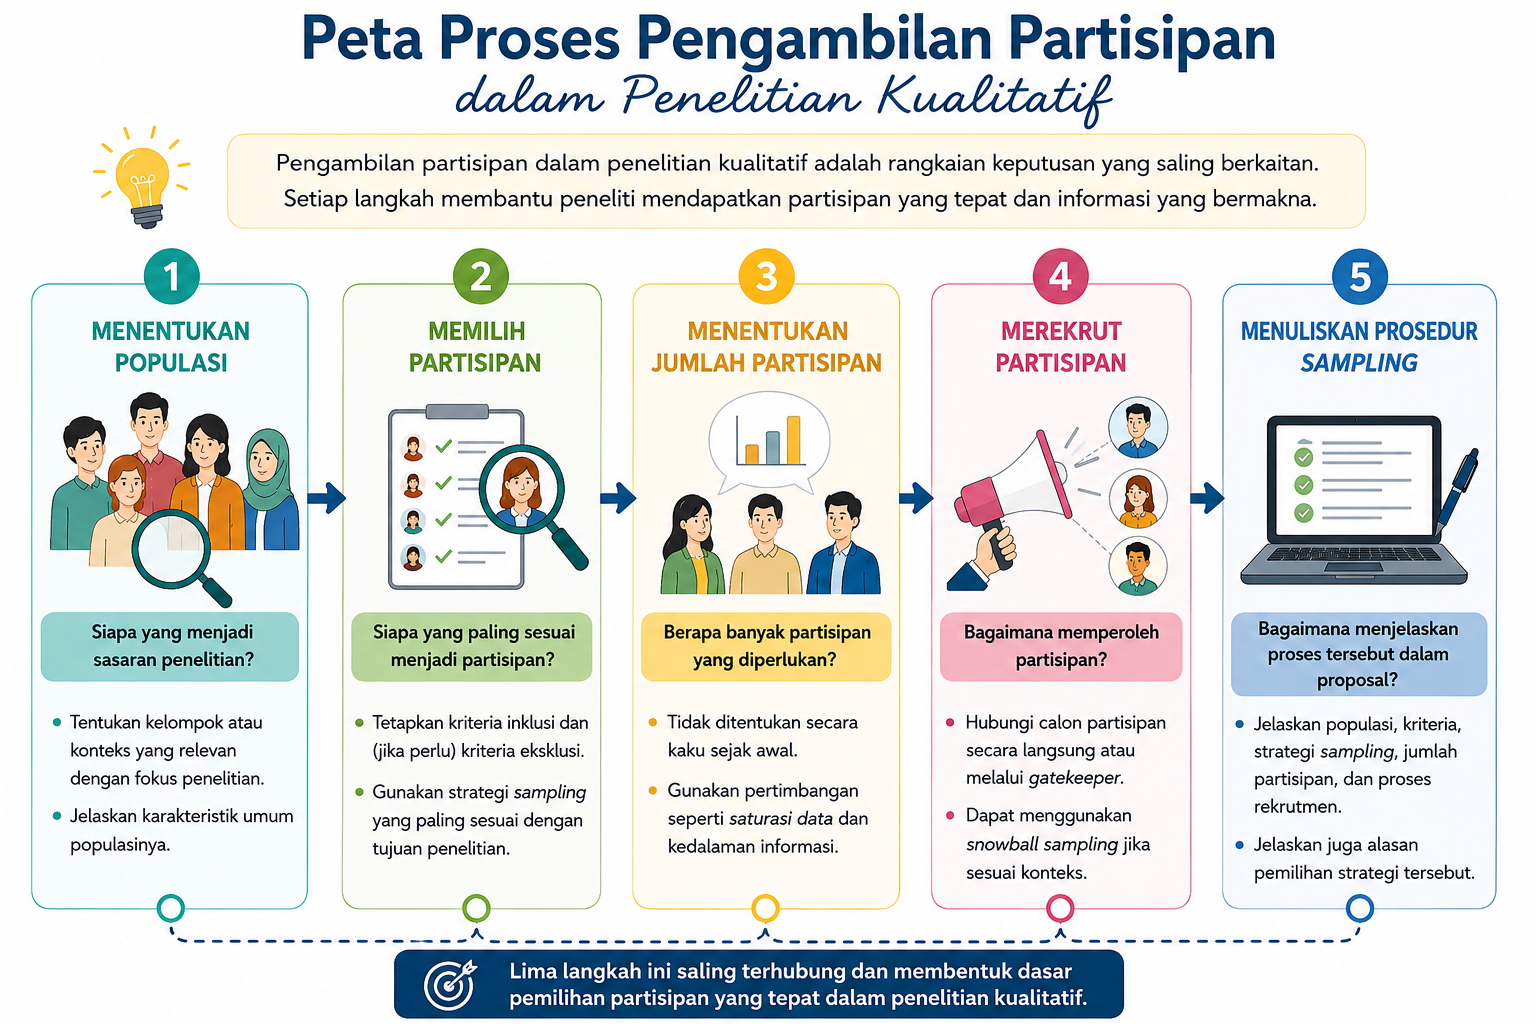
\includegraphics[keepaspectratio]{images/samplingkuali.png}}
\caption{Proses Pengambilan Partisipan dalam Penelitian Kualitatif}
\end{figure}

}

\caption{\label{fig-proseskuali}}

\end{figure}%

\begin{tcolorbox}[enhanced jigsaw, colframe=quarto-callout-tip-color-frame, toptitle=1mm, breakable, leftrule=.75mm, arc=.35mm, toprule=.15mm, colback=white, colbacktitle=quarto-callout-tip-color!10!white, bottomtitle=1mm, bottomrule=.15mm, titlerule=0mm, title=\textcolor{quarto-callout-tip-color}{\faLightbulb}\hspace{0.5em}{Rangkuman}, coltitle=black, left=2mm, opacitybacktitle=0.6, opacityback=0, rightrule=.15mm]

\begin{enumerate}
\def\labelenumi{\arabic{enumi}.}
\tightlist
\item
  Penelitian kualitatif menggunakan sampling untuk memperoleh partisipan
  yang mampu memberikan informasi secara mendalam mengenai fenomena yang
  diteliti.
\item
  Penentuan populasi diawali dengan menetapkan fokus penelitian serta
  kriteria inklusi dan eksklusi partisipan.
\item
  \emph{Purposive sampling} merupakan strategi sampling yang paling umum
  digunakan, dengan berbagai variasi yang disesuaikan dengan tujuan
  penelitian.
\item
  \emph{Snowball sampling} digunakan ketika populasi penelitian sulit
  dijangkau atau tidak memiliki daftar anggota yang jelas.
\item
  Jumlah partisipan ditentukan berdasarkan tujuan penelitian dan prinsip
  saturasi data, bukan berdasarkan rumus statistik.
\item
  Rekrutmen partisipan dapat dilakukan melalui berbagai cara sesuai
  dengan karakteristik populasi dan konteks penelitian.
\item
  Prosedur sampling perlu dilaporkan secara jelas agar proses penelitian
  dapat dipahami dan dipertanggungjawabkan.
\end{enumerate}

\end{tcolorbox}

\begin{tcolorbox}[enhanced jigsaw, colframe=quarto-callout-important-color-frame, toptitle=1mm, breakable, leftrule=.75mm, arc=.35mm, toprule=.15mm, colback=white, colbacktitle=quarto-callout-important-color!10!white, bottomtitle=1mm, bottomrule=.15mm, titlerule=0mm, title=\textcolor{quarto-callout-important-color}{\faExclamation}\hspace{0.5em}{Refleksi \& Diskusi}, coltitle=black, left=2mm, opacitybacktitle=0.6, opacityback=0, rightrule=.15mm]

\begin{itemize}
\tightlist
\item
  Mengapa penelitian kualitatif lebih menekankan pemilihan partisipan
  yang mampu memberikan informasi secara mendalam daripada keterwakilan
  populasi secara statistik?
\item
  Bayangkan Anda akan melakukan penelitian fenomenologi mengenai
  pengalaman mahasiswa yang mengalami \emph{academic burnout}. Siapa
  yang menjadi populasi penelitian? Kriteria inklusi dan eksklusi apa
  yang akan Anda tetapkan?
\item
  Suatu penelitian bertujuan mengeksplorasi pengalaman penggunaan
  kecerdasan artifisial (\emph{artificial intelligence}) dalam proses
  pembelajaran oleh mahasiswa dari berbagai program studi. Strategi
  \emph{purposive sampling} apa yang paling tepat digunakan? Jelaskan
  alasan Anda.
\item
  Dalam kondisi seperti apa \emph{snowball sampling} lebih tepat
  digunakan dibandingkan \emph{purposive sampling} biasa? Berikan contoh
  topik penelitian yang sesuai.
\item
  Seorang mahasiswa menyatakan bahwa penelitian kualitatif minimal harus
  melibatkan 30 partisipan agar hasilnya valid. Apakah Anda setuju
  dengan pernyataan tersebut? Jelaskan jawaban Anda berdasarkan konsep
  saturasi data.
\end{itemize}

\end{tcolorbox}

\phantomsection\label{refs--18}
\begin{CSLReferences}{1}{0}
\bibitem[\citeproctext]{ref-Bordens2018--18}
Bordens, K. S., \& Abbott, B. B. (2018). \emph{Research design and
methods: A process approach} (10th ed.). McGraw-Hill Education.

\bibitem[\citeproctext]{ref-Charmaz2014--18}
Charmaz, Kathy. (2014). \emph{Constructing grounded theory}. SAGE.

\bibitem[\citeproctext]{ref-Creswell2018a--18}
Creswell, J. W., \& Creswell, J. D. (2023). \emph{Research design:
Qualitative, quantitative, and mixed methods approaches} (6th ed.). SAGE
Publications.

\bibitem[\citeproctext]{ref-Guest2006--18}
Guest, G., Bunce, A., \& Johnson, L. (2006). How Many Interviews Are
Enough? \emph{Field Methods}, \emph{18}, 59--82.
\url{https://doi.org/10.1177/1525822X05279903}

\bibitem[\citeproctext]{ref-Hennink2017--18}
Hennink, M. M., Kaiser, B. N., \& Marconi, V. C. (2017). Code Saturation
Versus Meaning Saturation. \emph{Qualitative Health Research},
\emph{27}, 591--608. \url{https://doi.org/10.1177/1049732316665344}

\bibitem[\citeproctext]{ref-Morling2024--18}
Morling, B. (2024). \emph{Research methods in psychology : evaluating a
world of information} (4th ed.). W.W. Norton \& Company, Inc.

\bibitem[\citeproctext]{ref-Neuman2014--18}
Neuman, W. L. (2014). \emph{Social research methods: Qualitative and
quantitative approaches} (7th ed.). Pearson.

\bibitem[\citeproctext]{ref-Patton2014--18}
Patton, M. Q. (2014). \emph{Qualitative research \& evaluation methods:
Integrating theory and practice}. SAGE Publications, Inc.

\bibitem[\citeproctext]{ref-Robinson2014--18}
Robinson, O. C. (2014). Sampling in Interview-Based Qualitative
Research: A Theoretical and Practical Guide. \emph{Qualitative Research
in Psychology}, \emph{11}, 25--41.
\url{https://doi.org/10.1080/14780887.2013.801543}

\bibitem[\citeproctext]{ref-Smith2021--18}
Smith, J. A. A., Flowers, P., \& Larkin, M. (2021). \emph{Interpretative
Phenomenological Analysis}. Sage Publications, Inc.

\bibitem[\citeproctext]{ref-Strauss1998--18}
Strauss, A. L., \& Corbin, J. M. (1998). \emph{Basics of qualitative
research : techniques and procedures for developing grounded theory}.
Sage Publications.

\bibitem[\citeproctext]{ref-Yin2018--18}
Yin, R. K., \& Campbell, D. T. (2018). \emph{Case study research and
applications: Design and methods}. SAGE Publications, Inc.

\end{CSLReferences}

\chapter{Pengumpulan dan Analisis Data
Kualitatif}\label{pengumpulan-dan-analisis-data-kualitatif}

\begin{tcolorbox}[enhanced jigsaw, colframe=quarto-callout-note-color-frame, toptitle=1mm, breakable, leftrule=.75mm, arc=.35mm, toprule=.15mm, colback=white, colbacktitle=quarto-callout-note-color!10!white, bottomtitle=1mm, bottomrule=.15mm, titlerule=0mm, title=\textcolor{quarto-callout-note-color}{\faInfo}\hspace{0.5em}{Capaian Pembelajaran}, coltitle=black, left=2mm, opacitybacktitle=0.6, opacityback=0, rightrule=.15mm]

Setelah mempelajari bab ini, mahasiswa diharapkan mampu:

\begin{enumerate}
\def\labelenumi{\arabic{enumi}.}
\tightlist
\item
  Menjelaskan karakteristik berbagai teknik pengumpulan data dalam
  penelitian kualitatif sesuai dengan tujuan penelitian.
\item
  Memilih teknik pengumpulan data yang paling sesuai dengan pertanyaan
  penelitian dan konteks lapangan.
\item
  Menjelaskan tahapan umum analisis data kualitatif, mulai dari
  penyiapan data hingga pembentukan tema.
\item
  Memahami proses analisis tematik sebagai salah satu pendekatan yang
  umum digunakan dalam penelitian kualitatif.
\item
  Menjelaskan hubungan antara data, kode, kategori, tema, dan
  interpretasi dalam menghasilkan temuan penelitian.
\end{enumerate}

\end{tcolorbox}

Penelitian kualitatif bertujuan memahami makna di balik pengalaman,
perilaku, dan interaksi manusia dalam konteks tertentu. Oleh karena itu,
data yang dikumpulkan umumnya berupa narasi, percakapan, hasil
observasi, maupun dokumen yang memberikan gambaran mendalam mengenai
fenomena yang diteliti. Berbeda dengan penelitian kuantitatif yang
berfokus pada pengukuran, penelitian kualitatif menekankan pemahaman
terhadap perspektif dan pengalaman partisipan.

Bab ini membahas teknik-teknik pengumpulan data yang umum digunakan
dalam penelitian kualitatif serta gambaran umum proses analisis data,
khususnya analisis tematik. Pembahasan difokuskan pada konsep-konsep
dasar agar pembaca memahami alur pengumpulan, pengolahan, dan
interpretasi data kualitatif secara sistematis.

\section{Pengumpulan Data dalam Penelitian
Kualitatif}\label{pengumpulan-data-dalam-penelitian-kualitatif}

Pengumpulan data merupakan proses memperoleh informasi yang diperlukan
untuk memahami suatu fenomena dari perspektif partisipan. Berbeda dengan
penelitian kuantitatif yang umumnya menggunakan instrumen terstandar,
penelitian kualitatif mengandalkan interaksi langsung antara peneliti
dan sumber data. Oleh karena itu, peneliti berperan sebagai instrumen
utama yang menentukan kualitas data melalui kemampuan membangun hubungan
dengan partisipan, mengajukan pertanyaan yang relevan, serta mengamati
situasi penelitian secara cermat (Creswell \& Poth, 2023; Merriam \&
Tisdell, 2016).

Dalam penelitian kualitatif, proses pengumpulan data bersifat fleksibel
dan berkembang seiring dengan berlangsungnya penelitian. Informasi yang
diperoleh pada tahap awal dapat memunculkan pertanyaan baru sehingga
peneliti perlu menyesuaikan fokus pengumpulan data. Dengan demikian,
pengumpulan dan analisis data berlangsung secara berulang
(\emph{iterative process}) hingga diperoleh pemahaman yang memadai
mengenai fenomena yang diteliti (Miles dkk., 2020; Saldaña, 2025) (lihat
Gambar~\ref{fig-sikluskualitatif}).

\begin{figure}

\centering{

\begin{figure}
\centering
\pandocbounded{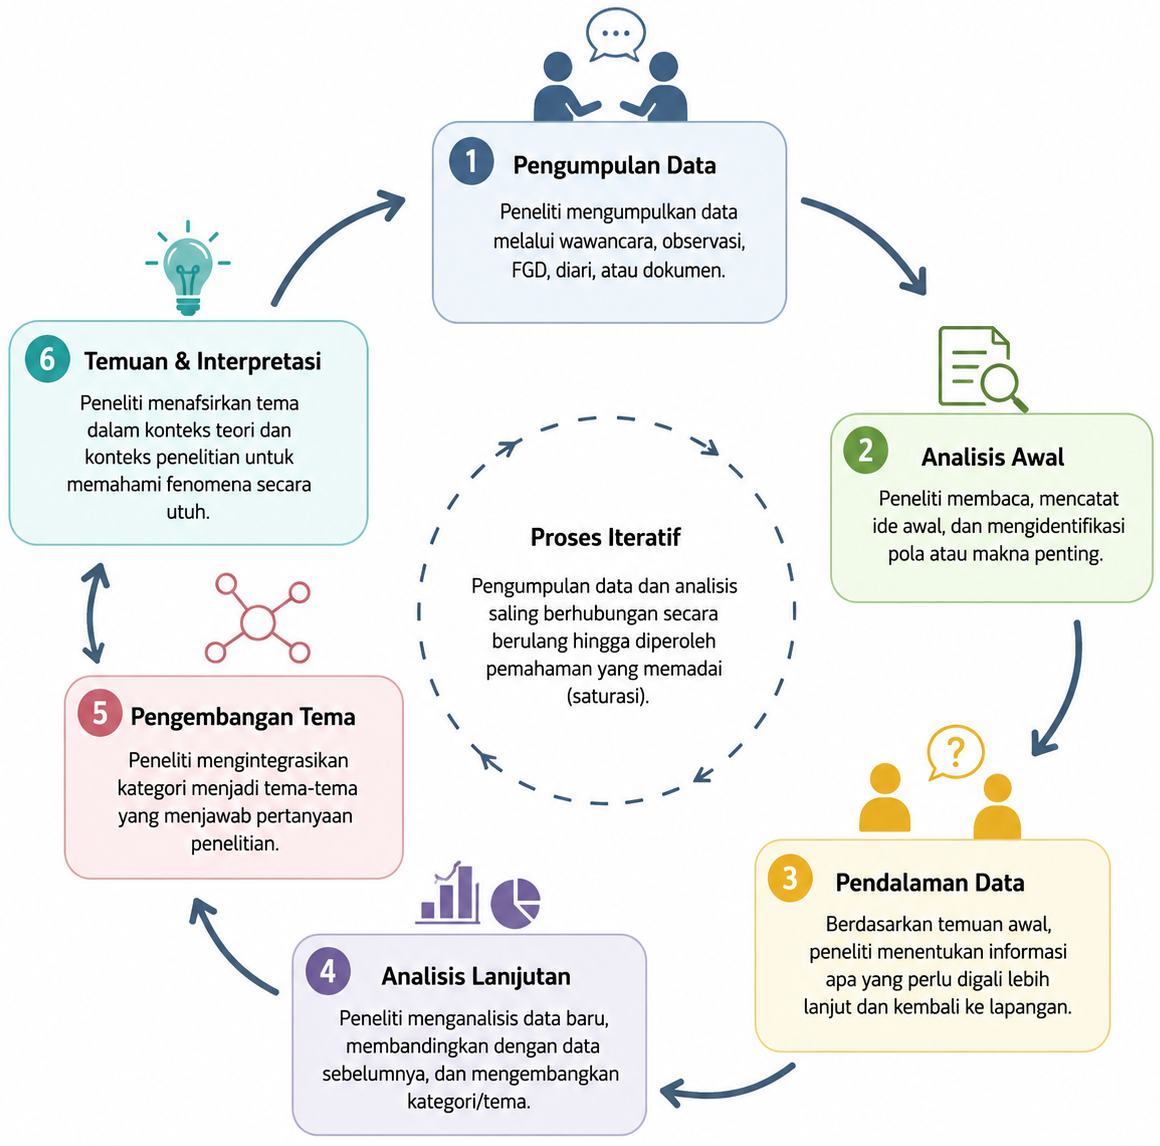
\includegraphics[keepaspectratio]{images/sikluskualitatif.png}}
\caption{Siklus Pengumpulan dan Analisis Data dalam Penelitian
Kualitatif}
\end{figure}

}

\caption{\label{fig-sikluskualitatif}}

\end{figure}%

\section{Teknik Pengumpulan Data
Kualitatif}\label{teknik-pengumpulan-data-kualitatif}

Berbagai teknik dapat digunakan untuk memperoleh data dalam penelitian
kualitatif. Pemilihan teknik bergantung pada tujuan penelitian,
karakteristik fenomena yang diteliti, serta jenis informasi yang ingin
diperoleh. Dalam praktiknya, peneliti sering mengombinasikan beberapa
teknik pengumpulan data untuk memperoleh pemahaman yang lebih
komprehensif mengenai suatu fenomena (Creswell \& Poth, 2023; Patton,
2014).

\subsection{Wawancara Mendalam}\label{wawancara-mendalam}

Wawancara mendalam (\emph{in-depth interview}) merupakan teknik
pengumpulan data melalui percakapan antara peneliti dan partisipan untuk
menggali pengalaman, pandangan, maupun makna yang mereka berikan
terhadap suatu fenomena. Teknik ini memungkinkan peneliti mengeksplorasi
perspektif partisipan secara lebih mendalam melalui pertanyaan yang
bersifat terbuka dan fleksibel (Brinkmann \& Kvale, 2018).

\subsection{Observasi}\label{observasi}

Observasi dilakukan dengan mengamati perilaku, aktivitas, interaksi,
maupun kondisi lingkungan tempat fenomena berlangsung. Teknik ini
membantu peneliti memahami fenomena dalam konteks alaminya sehingga
dapat melengkapi informasi yang diperoleh melalui wawancara. Observasi
dapat dilakukan dengan berbagai tingkat keterlibatan peneliti, mulai
dari pengamat hingga partisipan (Creswell \& Poth, 2023; Patton, 2014).

\subsection{\texorpdfstring{\emph{Focus Group Discussion}
(FGD)}{Focus Group Discussion (FGD)}}\label{focus-group-discussion-fgd}

\emph{Focus Group Discussion} (FGD) merupakan teknik pengumpulan data
melalui diskusi kelompok yang dipandu oleh seorang moderator. Selain
memperoleh berbagai sudut pandang dalam waktu yang relatif singkat, FGD
memungkinkan peneliti mengamati bagaimana peserta saling menanggapi,
menyepakati, atau mempertentangkan suatu isu sehingga dinamika sosial
menjadi bagian penting dari data penelitian (Krueger \& Casey, 2015).

\subsection{Diari dan Dokumen Pribadi}\label{diari-dan-dokumen-pribadi}

Diari dan dokumen pribadi dapat menjadi sumber data yang kaya mengenai
pengalaman sehari-hari partisipan. Catatan yang dibuat secara berkala
memungkinkan peneliti memahami perubahan pengalaman, emosi, maupun
aktivitas dalam konteks kehidupan nyata. Selain diari tertulis,
perkembangan teknologi juga memungkinkan penggunaan diari digital,
rekaman suara, maupun dokumentasi visual sebagai sumber data penelitian
(Alaszewski, 2006; Flick, 2022).

\begin{longtable}[]{@{}
  >{\raggedright\arraybackslash}p{(\linewidth - 8\tabcolsep) * \real{0.2000}}
  >{\raggedright\arraybackslash}p{(\linewidth - 8\tabcolsep) * \real{0.2000}}
  >{\raggedright\arraybackslash}p{(\linewidth - 8\tabcolsep) * \real{0.2000}}
  >{\raggedright\arraybackslash}p{(\linewidth - 8\tabcolsep) * \real{0.2000}}
  >{\raggedright\arraybackslash}p{(\linewidth - 8\tabcolsep) * \real{0.2000}}@{}}
\caption{Perbandingan teknik pengumpulan data
kualitatif}\label{tbl-teknikkuali}\tabularnewline
\toprule\noalign{}
\endfirsthead
\endhead
\bottomrule\noalign{}
\endlastfoot
\textbf{Teknik} & \textbf{Tujuan Utama} & \textbf{Jenis Data yang
Dihasilkan} & \textbf{Kelebihan} & \textbf{Keterbatasan} \\
\textbf{Wawancara mendalam} & Menggali pengalaman, persepsi, dan makna
yang dimiliki partisipan & Narasi hasil percakapan individual &
Menghasilkan data yang mendalam dan kaya makna; memungkinkan eksplorasi
lebih lanjut melalui pertanyaan lanjutan & Membutuhkan waktu yang
relatif lama dan sangat bergantung pada kemampuan pewawancara \\
\textbf{Observasi} & Memahami perilaku, interaksi, dan konteks secara
langsung & Catatan lapangan, foto, atau dokumentasi visual & Menangkap
perilaku dalam konteks alami; melengkapi data hasil wawancara & Tidak
semua fenomena dapat diamati secara langsung; interpretasi peneliti
dapat memengaruhi hasil observasi \\
\textbf{\emph{Focus Group Discussion}} \textbf{(FGD)} & Menggali
pandangan dan pengalaman melalui diskusi kelompok & Transkrip diskusi
kelompok dan dinamika interaksi peserta & Menghasilkan beragam
perspektif dalam waktu relatif singkat; memungkinkan munculnya ide
melalui interaksi antarpeserta & Diskusi dapat didominasi oleh peserta
tertentu; kurang sesuai untuk topik yang sangat sensitif atau
personal \\
\textbf{Diari atau dokumen pribadi} & Mendokumentasikan pengalaman dan
aktivitas secara berkelanjutan & Catatan harian, jurnal, rekaman suara,
foto, atau dokumen pribadi & Memberikan gambaran pengalaman secara
kronologis dan dalam konteks kehidupan sehari-hari & Bergantung pada
komitmen partisipan; kualitas data dapat bervariasi antarpartisipan \\
\end{longtable}

\section{Memilih Teknik Pengumpulan
Data}\label{memilih-teknik-pengumpulan-data}

Tidak ada satu teknik pengumpulan data yang paling tepat untuk semua
penelitian kualitatif. Pemilihan teknik harus disesuaikan dengan
pertanyaan penelitian, karakteristik partisipan, serta konteks
penelitian. Sebagai contoh, wawancara mendalam lebih sesuai untuk
memahami pengalaman individual, sedangkan FGD lebih tepat digunakan
ketika peneliti ingin mengeksplorasi persepsi atau pengalaman yang
berkembang dalam suatu kelompok. Observasi lebih bermanfaat ketika
perilaku dan interaksi sosial menjadi fokus penelitian, sedangkan diari
cocok digunakan untuk memahami pengalaman yang berlangsung secara
berkelanjutan (Creswell \& Poth, 2023; Patton, 2014).

Dalam banyak penelitian, penggunaan lebih dari satu teknik pengumpulan
data dapat menghasilkan pemahaman yang lebih utuh mengenai fenomena yang
diteliti. Kombinasi wawancara, observasi, maupun analisis dokumen
memungkinkan peneliti memperoleh informasi yang saling melengkapi
sehingga interpretasi terhadap data menjadi lebih kaya dan kredibel
(Lincoln \& Guba, 1985; Miles dkk., 2020).

\section{Menyiapkan Data untuk
Analisis}\label{menyiapkan-data-untuk-analisis}

Data yang diperoleh melalui wawancara, observasi, FGD, maupun dokumen
belum dapat langsung dianalisis. Peneliti perlu menyiapkan data agar
tersusun secara sistematis dan mudah ditelusuri selama proses analisis.
Tahap ini umumnya meliputi transkripsi rekaman, pengorganisasian berkas,
pemberian identitas atau kode pada partisipan, serta penyusunan catatan
lapangan. Pengelolaan data yang baik akan membantu menjaga
ketertelusuran proses analisis sekaligus meningkatkan transparansi
penelitian (Creswell \& Poth, 2023; Miles dkk., 2020).

Sebelum melakukan analisis yang lebih mendalam, peneliti juga perlu
membiasakan diri (\emph{familiarization}) dengan data melalui pembacaan
atau penelaahan berulang. Proses ini bertujuan memperoleh pemahaman
menyeluruh mengenai isi data, mengenali pola awal, serta mencatat ide
atau refleksi yang muncul selama membaca. Familiarisasi merupakan tahap
penting karena menjadi dasar dalam proses pengodean dan pengembangan
tema (Braun \& Clarke, 2006). Gambar~\ref{fig-penyiapandata}
mengIlustrasikan tahapan penyiapan data untuk analisis.

\begin{figure}

\centering{

\begin{figure}
\centering
\pandocbounded{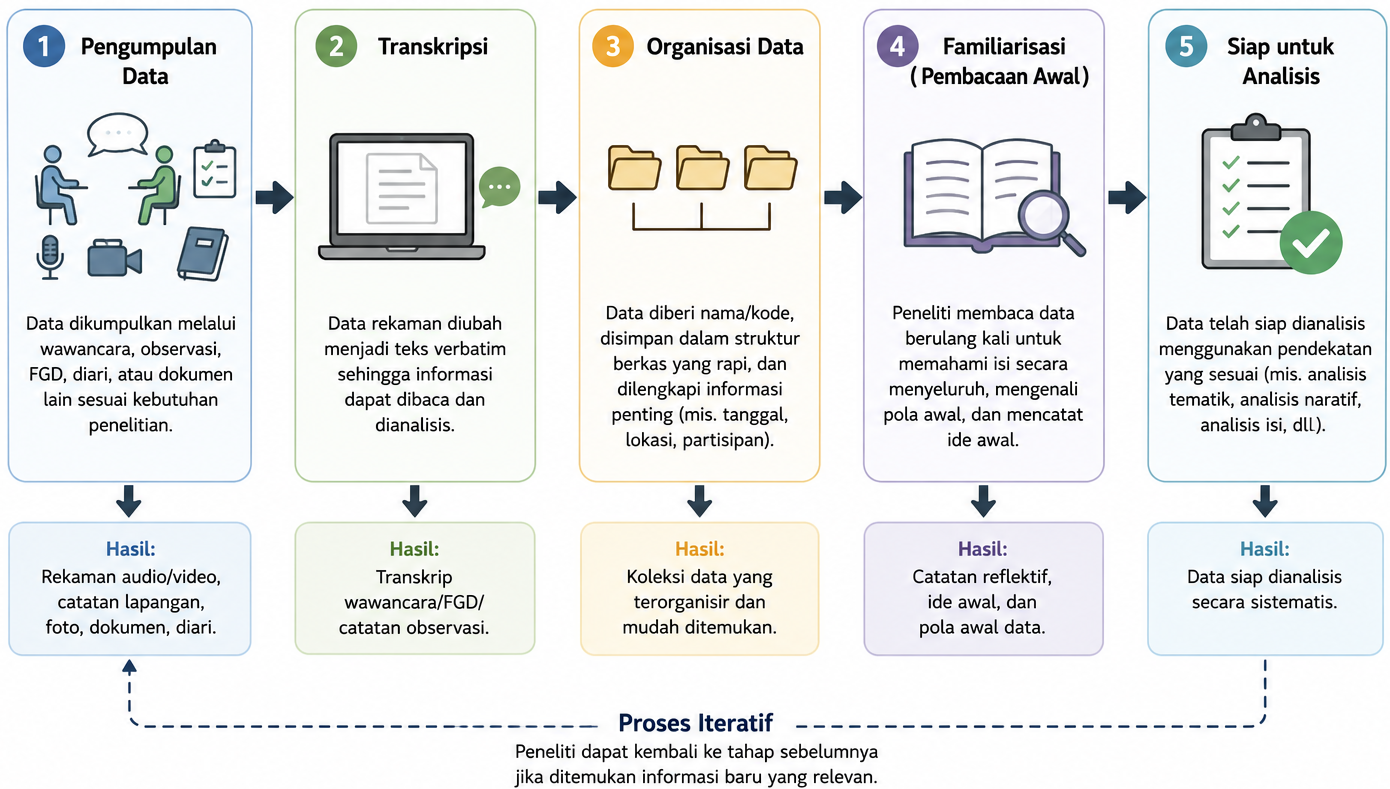
\includegraphics[keepaspectratio]{images/penyiapandata.png}}
\caption{Tahapan Penyiapan Data Kualitatif untuk Analisis}
\end{figure}

}

\caption{\label{fig-penyiapandata}}

\end{figure}%

\section{Analisis Tematik}\label{analisis-tematik}

Analisis tematik (\emph{thematic analysis}) merupakan salah satu
pendekatan analisis data kualitatif yang paling banyak digunakan karena
bersifat fleksibel dan dapat diterapkan pada berbagai desain penelitian.
Tujuan analisis tematik adalah mengidentifikasi, mengorganisasi, dan
menginterpretasikan pola makna (\emph{themes}) yang muncul dari data
sehingga peneliti dapat menjawab pertanyaan penelitian secara sistematis
(Braun \& Clarke, 2006).

Meskipun terdapat berbagai pendekatan analisis kualitatif, secara umum
analisis tematik dilakukan melalui empat tahapan utama: memahami data,
memberikan kode, mengembangkan kategori dan tema, serta
menginterpretasikan hasil analisis. Keempat tahapan tersebut tidak
selalu berlangsung secara linier, tetapi sering kali dilakukan secara
berulang hingga diperoleh tema yang benar-benar mencerminkan data.

\subsection{\texorpdfstring{Memberikan Kode
(\emph{Coding})}{Memberikan Kode (Coding)}}\label{memberikan-kode-coding}

Tahap pertama dalam analisis tematik adalah memberikan kode
(\emph{coding}) pada data. Kode merupakan label singkat yang diberikan
pada bagian-bagian data yang dianggap relevan dengan pertanyaan
penelitian. Melalui proses ini, data yang semula berupa narasi panjang
dipecah menjadi unit-unit makna yang lebih kecil sehingga lebih mudah
dikelompokkan dan dianalisis (Saldaña, 2025).

Pemberian kode bukan sekadar menandai kata atau kalimat tertentu, tetapi
merupakan proses mengidentifikasi informasi yang bermakna dalam data.
Satu kutipan dapat menghasilkan lebih dari satu kode apabila memuat
beberapa gagasan yang berbeda. Sebaliknya, beberapa kutipan dari
partisipan yang berbeda dapat memperoleh kode yang sama apabila
menggambarkan makna yang serupa. Oleh karena itu, proses coding menuntut
peneliti membaca data secara cermat, memahami konteks setiap pernyataan,
dan menghubungkannya dengan fokus penelitian (Braun \& Clarke, 2006).

Sebagai contoh, pernyataan partisipan ``Sejak merantau saya sering
merasa kesepian karena jauh dari keluarga'' dapat diberi kode
\textbf{merasa kesepian} dan \textbf{jauh dari keluarga}. Kedua kode
tersebut masih merupakan representasi awal dari data dan belum menjadi
kesimpulan penelitian.

\subsection{Mengembangkan Kategori dan
Tema}\label{mengembangkan-kategori-dan-tema}

\textbf{Menyusun Kategori}

Setelah seluruh data diberi kode, langkah berikutnya adalah
mengelompokkan kode-kode yang memiliki kesamaan makna ke dalam kategori.
Kategori merupakan kumpulan kode yang menggambarkan aspek atau
karakteristik tertentu dari fenomena yang sedang diteliti. Tujuan
kategorisasi adalah menyederhanakan sejumlah besar kode menjadi
kelompok-kelompok yang lebih terstruktur sehingga pola dalam data mulai
terlihat (Miles dkk., 2020).

Sebagai contoh, kode \textbf{merasa kesepian}, \textbf{tidak memiliki
teman dekat}, dan \textbf{sulit menyesuaikan diri} dapat dikelompokkan
ke dalam kategori \textbf{tantangan adaptasi sosial}. Demikian pula,
kode \textbf{mendapat dukungan teman}, \textbf{bergabung dengan
organisasi}, dan \textbf{memiliki lingkungan yang suportif} dapat
membentuk kategori \textbf{dukungan sosial}.

\textbf{Mengembangkan Tema}

Langkah berikutnya adalah mengembangkan tema (\emph{theme}), yaitu pola
makna yang lebih luas yang terbentuk dari hubungan antarkategori. Jika
kategori menggambarkan aspek-aspek tertentu dari suatu fenomena, maka
tema menjelaskan bagaimana aspek-aspek tersebut saling berkaitan untuk
menjawab pertanyaan penelitian. Dengan demikian, tema tidak hanya
merangkum data, tetapi juga memberikan penjelasan mengenai makna yang
terkandung di dalamnya (Braun \& Clarke, 2006).

Sebagai ilustrasi, kategori \textbf{tantangan adaptasi sosial},
\textbf{dukungan sosial}, dan \textbf{penyesuaian diri} dapat
diintegrasikan menjadi tema \textbf{proses adaptasi mahasiswa perantau}.
Tema inilah yang kemudian menjadi dasar bagi peneliti dalam menyusun
narasi hasil penelitian. Hubungan antara data, kode, kategori, dan tema
ditunjukkan pada Gambar~\ref{fig-datakuali}.

\begin{figure}

\centering{

\begin{figure}
\centering
\pandocbounded{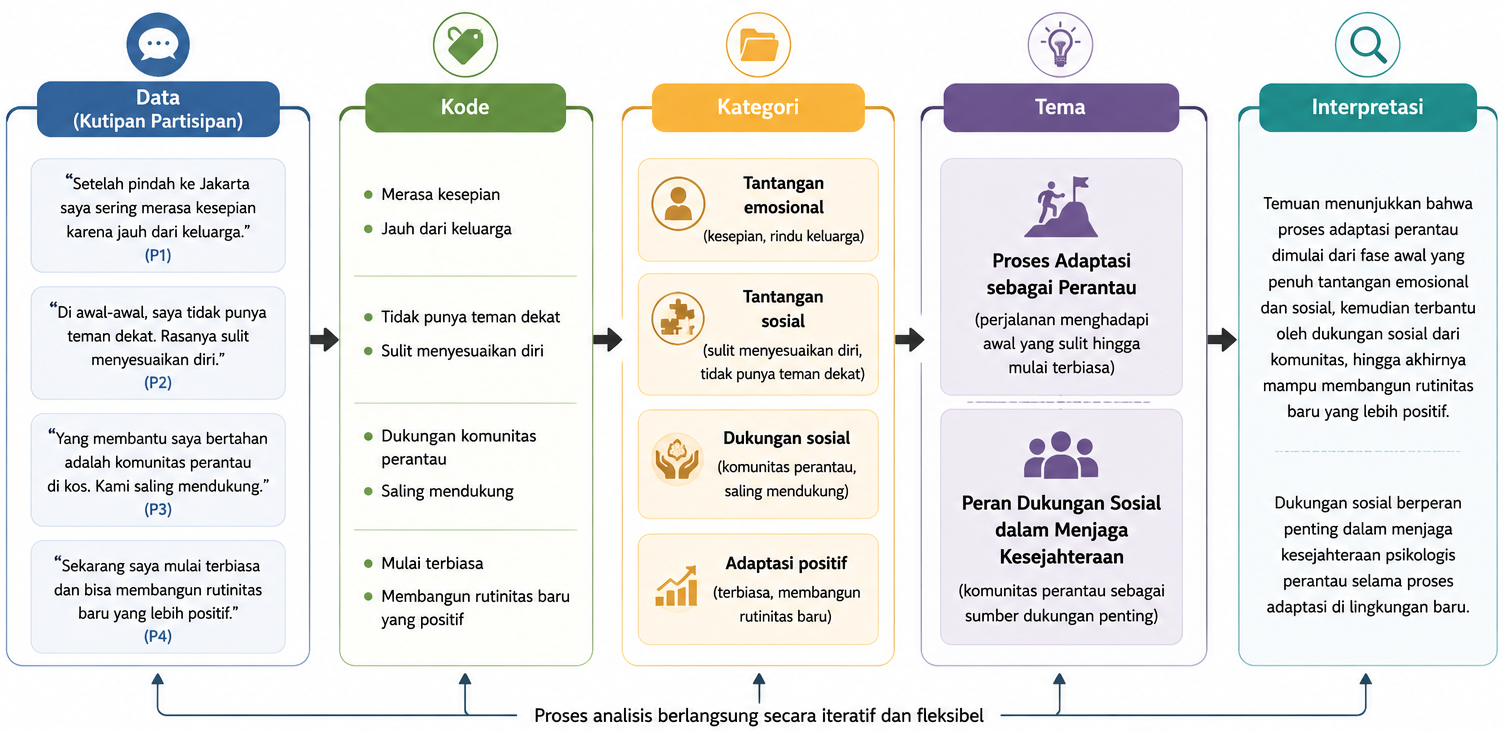
\includegraphics[keepaspectratio]{images/datakuali.png}}
\caption{Contoh Hubungan antara Data, Kode, Kategori, \& Tema}
\end{figure}

}

\caption{\label{fig-datakuali}}

\end{figure}%

\section{Interpretasi Data
Kualitatif}\label{interpretasi-data-kualitatif}

Interpretasi merupakan tahap akhir dalam analisis data kualitatif, yaitu
proses memberikan makna terhadap tema-tema yang telah diperoleh. Pada
tahap ini, peneliti tidak hanya mendeskripsikan apa yang disampaikan
oleh partisipan, tetapi juga menjelaskan bagaimana temuan tersebut
menjawab pertanyaan penelitian serta apa implikasinya dalam konteks
teori maupun penelitian terdahulu (Creswell \& Poth, 2023; Merriam \&
Tisdell, 2016).

Interpretasi harus didasarkan pada bukti yang memadai dari data. Oleh
karena itu, setiap tema umumnya didukung oleh kutipan partisipan, hasil
observasi, maupun dokumen yang relevan. Kutipan tersebut berfungsi
sebagai bukti empiris yang menunjukkan bahwa interpretasi yang dibuat
benar-benar berakar pada data, bukan semata-mata merupakan asumsi
peneliti (Patton, 2014).

Interpretasi juga tidak berhenti pada tahap mendeskripsikan tema.
Peneliti perlu menjelaskan hubungan antartema, mengaitkannya dengan
konteks penelitian, serta menunjukkan bagaimana temuan tersebut
berkontribusi terhadap pemahaman mengenai fenomena yang diteliti. Dengan
demikian, hasil penelitian tidak hanya menjawab pertanyaan penelitian,
tetapi juga menghasilkan pengetahuan baru atau memperkaya pengetahuan
yang telah ada.

Karena interpretasi sangat dipengaruhi oleh cara peneliti memahami dan
memaknai data, proses ini perlu dilakukan secara sistematis, transparan,
dan reflektif. Berbagai strategi untuk menjaga kredibilitas interpretasi
akan dibahas lebih lanjut pada Bab~\ref{sec-keabsahan}.

\begin{tcolorbox}[enhanced jigsaw, colframe=quarto-callout-tip-color-frame, toptitle=1mm, breakable, leftrule=.75mm, arc=.35mm, toprule=.15mm, colback=white, colbacktitle=quarto-callout-tip-color!10!white, bottomtitle=1mm, bottomrule=.15mm, titlerule=0mm, title=\textcolor{quarto-callout-tip-color}{\faLightbulb}\hspace{0.5em}{Rangkuman}, coltitle=black, left=2mm, opacitybacktitle=0.6, opacityback=0, rightrule=.15mm]

\begin{enumerate}
\def\labelenumi{\arabic{enumi}.}
\tightlist
\item
  Penelitian kualitatif mengumpulkan data yang kaya makna melalui
  berbagai teknik, seperti wawancara mendalam, observasi, \emph{focus
  group discussion} (FGD), dan diari atau dokumen pribadi.
\item
  Pemilihan teknik pengumpulan data harus disesuaikan dengan tujuan
  penelitian, karakteristik partisipan, serta jenis informasi yang ingin
  diperoleh.
\item
  Sebelum dianalisis, data perlu dipersiapkan melalui proses
  transkripsi, pengorganisasian, dan familiarisasi agar peneliti
  memahami konteks serta isi data secara menyeluruh.
\item
  Analisis tematik dilakukan dengan mengidentifikasi kode,
  mengelompokkannya ke dalam kategori, kemudian mengembangkan tema yang
  menjelaskan pola makna dalam data.
\item
  Interpretasi merupakan proses memberi makna terhadap tema-tema yang
  ditemukan dengan mengaitkannya pada pertanyaan penelitian, teori, dan
  hasil penelitian sebelumnya.
\item
  Pengumpulan dan analisis data dalam penelitian kualitatif merupakan
  proses yang bersifat iteratif, sehingga keduanya saling memengaruhi
  selama penelitian berlangsung.
\end{enumerate}

\end{tcolorbox}

\begin{tcolorbox}[enhanced jigsaw, colframe=quarto-callout-important-color-frame, toptitle=1mm, breakable, leftrule=.75mm, arc=.35mm, toprule=.15mm, colback=white, colbacktitle=quarto-callout-important-color!10!white, bottomtitle=1mm, bottomrule=.15mm, titlerule=0mm, title=\textcolor{quarto-callout-important-color}{\faExclamation}\hspace{0.5em}{Refleksi \& Diskusi}, coltitle=black, left=2mm, opacitybacktitle=0.6, opacityback=0, rightrule=.15mm]

\begin{itemize}
\tightlist
\item
  Mengapa proses pengumpulan dan analisis data dalam penelitian
  kualitatif bersifat iteratif? Jelaskan implikasinya terhadap
  pelaksanaan penelitian.
\item
  Jika Anda ingin memahami pengalaman mahasiswa baru dalam beradaptasi
  dengan kehidupan kampus, teknik pengumpulan data apa yang paling
  sesuai? Jelaskan alasan pemilihan Anda.
\item
  Mengapa proses \emph{coding} tidak dapat disamakan dengan sekadar
  memberi label pada data? Diskusikan peran \emph{coding} dalam
  membangun tema penelitian.
\item
  Apa perbedaan antara kode, kategori, dan tema dalam analisis tematik?
  Berikan ilustrasi sederhana untuk menjelaskan hubungan ketiganya.
\item
  Menurut Anda, mengapa interpretasi dalam penelitian kualitatif harus
  selalu didukung oleh bukti yang berasal dari data?
\end{itemize}

\end{tcolorbox}

\phantomsection\label{refs--19}
\begin{CSLReferences}{1}{0}
\bibitem[\citeproctext]{ref-Alaszewski2006--19}
Alaszewski, A. (2006). \emph{Using Diaries for Social Research}. SAGE
Publications Ltd. \url{https://doi.org/10.4135/9780857020215}

\bibitem[\citeproctext]{ref-Braun2006--19}
Braun, V., \& Clarke, V. (2006). Using thematic analysis in psychology.
\emph{Qualitative Research in Psychology}, \emph{3}, 77--101.
\url{https://doi.org/10.1191/1478088706qp063oa}

\bibitem[\citeproctext]{ref-Brinkmann2018--19}
Brinkmann, S., \& Kvale, S. (2018). \emph{Doing Interviews}. SAGE
Publications Ltd. \url{https://doi.org/10.4135/9781529716665}

\bibitem[\citeproctext]{ref-Creswell2023--19}
Creswell, J. W., \& Poth, C. N. (2023). \emph{Qualitative inquiry \&
research design: Choosing among five approaches} (5th ed.). SAGE
Publications, Inc.

\bibitem[\citeproctext]{ref-Flick2022--19}
Flick, U. (2022). \emph{An introduction to qualitative research} (7th
ed.). SAGE Publications Ltd.

\bibitem[\citeproctext]{ref-Krueger2015--19}
Krueger, R. A., \& Casey, M. A. (2015). \emph{Focus groups: a practical
guide for applied research} (5th ed.). SAGE.

\bibitem[\citeproctext]{ref-Lincoln1990--19}
Lincoln, Y. S., \& Guba, E. G. (1985). \emph{Naturalistic inquiry}.
Sage.

\bibitem[\citeproctext]{ref-Merriam2016--19}
Merriam, S. B., \& Tisdell, E. J. (2016). \emph{Qualitative research: A
guide to design and implementation}. John Wiley \& Sons.

\bibitem[\citeproctext]{ref-Miles2020--19}
Miles, M. B., Huberman, A. M., \& Saldaña, J. (2020). \emph{Qualitative
data analysis: a methods sourcebook} (4th ed.). SAGE.

\bibitem[\citeproctext]{ref-Patton2014--19}
Patton, M. Q. (2014). \emph{Qualitative research \& evaluation methods:
Integrating theory and practice}. SAGE Publications, Inc.

\bibitem[\citeproctext]{ref-Saldana2025--19}
Saldaña, J. (2025). \emph{The coding manual for qualitative researchers}
(5th ed.). Sage.

\end{CSLReferences}

\chapter{Keabsahan \& Refleksivitas Penelitian
Kualitatif}\label{sec-keabsahan}

\begin{tcolorbox}[enhanced jigsaw, colframe=quarto-callout-note-color-frame, toptitle=1mm, breakable, leftrule=.75mm, arc=.35mm, toprule=.15mm, colback=white, colbacktitle=quarto-callout-note-color!10!white, bottomtitle=1mm, bottomrule=.15mm, titlerule=0mm, title=\textcolor{quarto-callout-note-color}{\faInfo}\hspace{0.5em}{Capaian Pembelajaran}, coltitle=black, left=2mm, opacitybacktitle=0.6, opacityback=0, rightrule=.15mm]

Setelah mempelajari bab ini, mahasiswa diharapkan mampu:

\begin{enumerate}
\def\labelenumi{\arabic{enumi}.}
\tightlist
\item
  Menjelaskan konsep keabsahan (\emph{trustworthiness}) dan
  refleksivitas (\emph{reflexivity}) dalam penelitian kualitatif.
\item
  Membedakan empat kriteria \emph{trustworthiness} (\emph{credibility,
  transferability, dependability,} dan \emph{confirmability}) beserta
  strategi yang digunakan untuk meningkatkannya.
\item
  Menjelaskan pentingnya refleksivitas serta pengaruh posisi
  (\emph{positionality}) peneliti terhadap proses dan hasil penelitian
  kualitatif.
\item
  Menerapkan strategi untuk menjaga keabsahan dan refleksivitas serta
  melaporkannya dalam proposal atau laporan penelitian kualitatif.
\end{enumerate}

\end{tcolorbox}

Penelitian kualitatif bertujuan memahami makna, pengalaman, dan fenomena
sosial dalam konteks tertentu. Oleh karena itu, kualitas penelitian
kualitatif tidak dapat dinilai hanya menggunakan konsep validitas dan
reliabilitas sebagaimana dalam penelitian kuantitatif. Sebagai gantinya,
penelitian kualitatif menggunakan konsep \emph{trustworthiness}
(keabsahan) untuk menilai sejauh mana proses dan temuan penelitian dapat
dipercaya, dilakukan secara sistematis, serta didukung oleh bukti yang
memadai.

Selain menjaga keabsahan, peneliti juga perlu menerapkan refleksivitas
(\emph{reflexivity}), yaitu kesadaran untuk merefleksikan bagaimana
latar belakang, pengalaman, nilai, dan posisi peneliti dapat memengaruhi
proses maupun hasil penelitian. Bab ini membahas konsep
\emph{trustworthiness} beserta strategi untuk meningkatkannya,
pentingnya refleksivitas dalam penelitian kualitatif, serta cara
melaporkan upaya menjaga keabsahan dan refleksivitas dalam proposal
maupun laporan penelitian.

\section{\texorpdfstring{Keabsahan (\emph{Trustworthiness}) dalam
Penelitian
Kualitatif}{Keabsahan (Trustworthiness) dalam Penelitian Kualitatif}}\label{sec-trustworthiness}

Penelitian kualitatif bertujuan memahami makna, pengalaman, dan realitas
sosial berdasarkan perspektif partisipan dalam konteks tertentu. Oleh
karena itu, kualitas penelitian kualitatif tidak dapat dinilai hanya
menggunakan konsep validitas dan reliabilitas yang lazim digunakan dalam
penelitian kuantitatif. Meskipun kedua pendekatan sama-sama mengutamakan
penelitian yang berkualitas, cara menilai kualitas tersebut disesuaikan
dengan karakteristik, tujuan, dan paradigma masing-masing pendekatan.

Dalam penelitian kualitatif, kualitas penelitian umumnya dinilai
menggunakan konsep \emph{trustworthiness}, yaitu sejauh mana proses dan
temuan penelitian dapat dipercaya (\emph{trustworthy}) serta didukung
oleh prosedur penelitian yang sistematis dan transparan. Konsep ini
diperkenalkan oleh Lincoln \& Guba (1985) sebagai alternatif terhadap
konsep validitas dan reliabilitas dalam penelitian kuantitatif.
\emph{Trustworthiness} menekankan bahwa kualitas penelitian tidak hanya
ditentukan oleh hasil akhir, tetapi juga oleh bagaimana data
dikumpulkan, dianalisis, diinterpretasikan, dan didokumentasikan selama
proses penelitian. Gambar~\ref{fig-trustworthiness} menyajikan
perbandingan konseptual antara standar keabsahan yang digunakan dalam
penelitian kuantitatif dan penelitian kualitatif.

\begin{figure}

\centering{

\begin{figure}
\centering
\pandocbounded{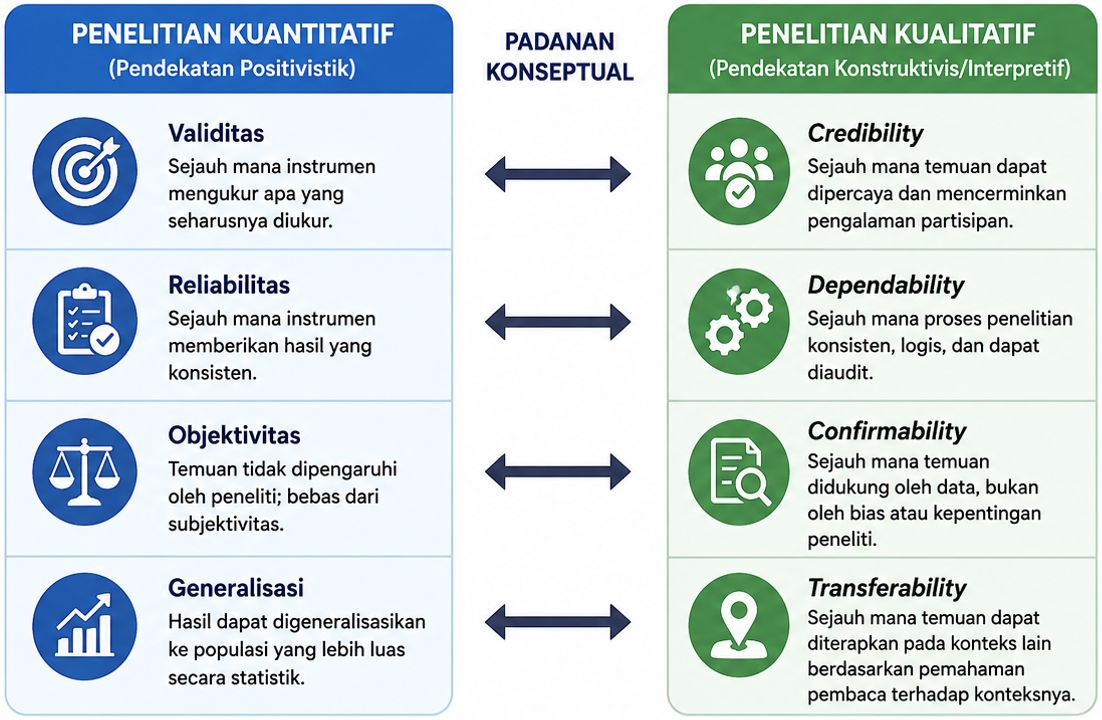
\includegraphics[keepaspectratio]{images/trustworthiness.png}}
\caption{Perbandingan konseptual keabsahan penelitian kuantitatif \&
kualitatif}
\end{figure}

}

\caption{\label{fig-trustworthiness}}

\end{figure}%

\subsection{\texorpdfstring{Kriteria
\emph{Trustworthiness}}{Kriteria Trustworthiness}}\label{sec-kriteria}

Lincoln \& Guba (1985) mengemukakan bahwa keabsahan
(\emph{trustworthiness}) dalam penelitian kualitatif terdiri atas empat
kriteria utama, yaitu \emph{credibility, transferability,
dependability}, dan \emph{confirmability}. Keempat kriteria tersebut
saling melengkapi dalam memastikan bahwa temuan penelitian benar-benar
mencerminkan pengalaman partisipan, didukung oleh proses penelitian yang
konsisten, serta dapat dipertanggungjawabkan secara ilmiah. Ringkasan
keempat kriteria tersebut disajikan pada
Tabel~\ref{tbl-trustworthiness}.

\begin{longtable}[]{@{}
  >{\raggedright\arraybackslash}p{(\linewidth - 6\tabcolsep) * \real{0.2500}}
  >{\raggedright\arraybackslash}p{(\linewidth - 6\tabcolsep) * \real{0.2500}}
  >{\raggedright\arraybackslash}p{(\linewidth - 6\tabcolsep) * \real{0.2500}}
  >{\raggedright\arraybackslash}p{(\linewidth - 6\tabcolsep) * \real{0.2500}}@{}}
\caption{Kriteria
\emph{trustworthiness}}\label{tbl-trustworthiness}\tabularnewline
\toprule\noalign{}
\endfirsthead
\endhead
\bottomrule\noalign{}
\endlastfoot
\textbf{Kriteria} & \textbf{Fokus Penilaian} & \textbf{Pertanyaan yang
Dijawab} & \textbf{Contoh Strategi} \\
\emph{Credibility} & Keterpercayaan temuan & Apakah temuan benar-benar
mencerminkan pengalaman atau perspektif partisipan? & Triangulasi,
\emph{member checking}, \emph{peer debriefing}, \emph{prolonged
engagement} \\
\emph{Transferability} & Keteralihan hasil penelitian & Apakah pembaca
memiliki informasi yang cukup untuk menilai apakah temuan relevan dengan
konteks lain? & \emph{Thick description} \\
\emph{Dependability} & Konsistensi proses penelitian & Apakah proses
penelitian dilakukan secara sistematis, logis, dan dapat ditelusuri? &
\emph{Audit trail}, dokumentasi proses \\
\emph{Confirmability} & Objektivitas interpretasi & Apakah temuan
didasarkan pada data, bukan semata-mata pada asumsi atau bias peneliti?
& \emph{Audit trail}, jurnal reflektif, triangulasi \\
\end{longtable}

\subsubsection{\texorpdfstring{\emph{Credibility}}{Credibility}}\label{credibility}

\emph{Credibility} mengacu pada tingkat keterpercayaan temuan penelitian
dalam merepresentasikan pengalaman, perspektif, atau realitas yang
disampaikan oleh partisipan. Dengan kata lain, kriteria ini menilai
sejauh mana interpretasi peneliti sesuai dengan makna yang dimaksud oleh
partisipan, sehingga temuan yang dihasilkan dipandang masuk akal dan
dapat dipercaya (Lincoln \& Guba, 1985). Dalam penelitian kualitatif,
\emph{credibility} sering dipandang sebagai kriteria yang paling penting
karena berkaitan langsung dengan kualitas interpretasi data.

Untuk meningkatkan \emph{credibility}, peneliti dapat menerapkan
berbagai strategi, seperti triangulasi, \emph{member checking},
\emph{peer debriefing}, dan \emph{prolonged engagement}.
Strategi-strategi tersebut bertujuan memastikan bahwa interpretasi
peneliti didasarkan pada data yang memadai dan memperoleh konfirmasi
dari berbagai sumber maupun pihak yang terlibat (Creswell \& Poth,
2023). Pembahasan lebih rinci mengenai strategi tersebut akan disajikan
pada Bab~\ref{sec-strategi}.

\subsubsection{\texorpdfstring{\emph{Transferability}}{Transferability}}\label{transferability}

\emph{Transferability} merujuk pada sejauh mana temuan penelitian dapat
dipahami dan dipertimbangkan relevansinya oleh pembaca untuk diterapkan
pada konteks lain yang memiliki karakteristik serupa. Berbeda dengan
penelitian kuantitatif yang menekankan generalisasi statistik,
penelitian kualitatif tidak bertujuan menggeneralisasikan hasil
penelitian kepada populasi yang lebih luas. Sebaliknya, penelitian
kualitatif menguraikan deskripsi konteks yang kaya sehingga pembaca
dapat menilai sendiri apakah temuan tersebut sesuai dengan situasi yang
dihadapinya (Lincoln \& Guba, 1985).

Oleh karena itu, tanggung jawab peneliti bukanlah membuktikan bahwa
hasil penelitiannya berlaku untuk semua konteks, melainkan menyajikan
informasi yang cukup mengenai karakteristik partisipan, latar
penelitian, serta proses penelitian. Salah satu strategi yang umum
digunakan untuk mendukung \emph{transferability} adalah \emph{thick
description}, yaitu penyajian deskripsi yang rinci mengenai konteks
penelitian (Creswell \& Poth, 2023).

\subsubsection{\texorpdfstring{\emph{Dependability}}{Dependability}}\label{dependability}

\emph{Dependability} berkaitan dengan konsistensi dan keterlacakan
proses penelitian. Kriteria ini menekankan bahwa setiap tahapan
penelitian, mulai dari perumusan pertanyaan penelitian, pengumpulan
data, analisis data, hingga penarikan kesimpulan, dilakukan secara
sistematis, logis, dan terdokumentasi dengan baik. Dengan demikian,
pembaca atau peneliti lain dapat memahami bagaimana suatu temuan
dihasilkan, meskipun hasil penelitian kualitatif tidak dimaksudkan untuk
direplikasi secara identik seperti pada penelitian kuantitatif (Lincoln
\& Guba, 1985).

Untuk mendukung \emph{dependability}, peneliti perlu mendokumentasikan
seluruh proses penelitian secara jelas, misalnya melalui \emph{audit
trail} atau dokumentasi keputusan metodologis yang diambil selama
penelitian berlangsung (Shenton, 2004). Dokumentasi tersebut menunjukkan
bahwa perubahan yang terjadi selama penelitian dilakukan secara sadar,
dapat dijelaskan, dan sesuai dengan perkembangan data di lapangan.

\subsubsection{\texorpdfstring{\emph{Confirmability}}{Confirmability}}\label{confirmability}

\emph{Confirmability} menunjukkan bahwa temuan penelitian didasarkan
pada data yang diperoleh dari partisipan, bukan semata-mata pada asumsi,
preferensi, atau bias peneliti. Dalam penelitian kualitatif, peneliti
memang menjadi instrumen utama penelitian sehingga subjektivitas tidak
dapat dihilangkan sepenuhnya. Namun, peneliti perlu menunjukkan bahwa
interpretasi yang dihasilkan memiliki dasar yang jelas dan dapat
ditelusuri kembali kepada data penelitian (Lincoln \& Guba, 1985).

Upaya untuk meningkatkan \emph{confirmability} dapat dilakukan melalui
dokumentasi proses penelitian, penyimpanan jejak analisis (\emph{audit
trail}), serta penerapan refleksivitas untuk menyadari bagaimana posisi
dan pengalaman peneliti dapat memengaruhi proses penelitian (Olmos-Vega
dkk., 2023; Shenton, 2004). Dengan demikian, pembaca dapat menilai bahwa
kesimpulan penelitian dibangun berdasarkan bukti empiris yang memadai
dan bukan semata-mata merupakan pendapat peneliti.

\subsection{\texorpdfstring{Strategi Meningkatkan
\emph{Trustworthiness}}{Strategi Meningkatkan Trustworthiness}}\label{sec-strategi}

Keempat kriteria \emph{trustworthiness} tidak dapat dicapai hanya dengan
memahami konsepnya, tetapi perlu didukung oleh berbagai strategi selama
proses penelitian. Strategi-strategi ini membantu peneliti memastikan
bahwa data dikumpulkan secara memadai, dianalisis secara sistematis, dan
diinterpretasikan secara bertanggung jawab. Pemilihan strategi yang
digunakan perlu disesuaikan dengan tujuan, desain, dan konteks
penelitian. Beberapa strategi yang paling umum diterapkan dalam
penelitian kualitatif dijelaskan sebagai berikut.

\subsubsection{\texorpdfstring{Triangulasi
(\emph{Triangulation})}{Triangulasi (Triangulation)}}\label{triangulasi-triangulation}

Triangulasi merupakan strategi untuk meningkatkan kepercayaan terhadap
temuan penelitian dengan membandingkan informasi yang diperoleh dari
berbagai sudut pandang. Kesesuaian informasi dari berbagai sumber atau
metode memberikan keyakinan yang lebih besar bahwa temuan tidak
bergantung pada satu sumber data saja Patton (2014).

Beberapa bentuk triangulasi yang umum digunakan meliputi:

\begin{itemize}
\tightlist
\item
  \textbf{Triangulasi sumber}, yaitu membandingkan informasi yang
  diperoleh dari partisipan atau sumber data yang berbeda.
\item
  \textbf{Triangulasi metode}, yaitu menggunakan lebih dari satu teknik
  pengumpulan data, misalnya wawancara, observasi, dan analisis dokumen.
\item
  \textbf{Triangulasi peneliti}, yaitu melibatkan lebih dari satu
  peneliti dalam proses pengumpulan atau analisis data.
\item
  \textbf{Triangulasi teori}, yaitu menggunakan lebih dari satu
  perspektif teoretis untuk menafsirkan data.
\end{itemize}

\begin{quote}
\textbf{Contoh:} Peneliti yang mengkaji pengalaman mahasiswa baru dapat
menggabungkan wawancara mendalam, observasi kegiatan orientasi, dan
analisis buku panduan akademik untuk memperoleh pemahaman yang lebih
komprehensif.
\end{quote}

\subsubsection{\texorpdfstring{\emph{Member
Checking}}{Member Checking}}\label{member-checking}

\emph{Member checking} merupakan proses meminta partisipan untuk
meninjau kembali hasil wawancara, ringkasan data, atau interpretasi
peneliti guna memastikan bahwa temuan telah menggambarkan pengalaman
mereka secara akurat (Creswell \& Poth, 2023). Strategi ini membantu
mengurangi kesalahan interpretasi dan meningkatkan \emph{credibility}.

\emph{Member checking} tidak selalu berarti meminta partisipan membaca
seluruh laporan penelitian. Peneliti dapat meminta tanggapan terhadap
ringkasan hasil wawancara, tema-tema awal, atau interpretasi tertentu
yang dianggap penting.

\subsubsection{\texorpdfstring{\emph{Audit
Trail}}{Audit Trail}}\label{audit-trail}

\emph{Audit trail} adalah dokumentasi sistematis mengenai seluruh proses
penelitian, mulai dari perencanaan, pengumpulan data, analisis, hingga
penarikan kesimpulan (Lincoln \& Guba, 1985). Dokumentasi ini
memungkinkan pembaca atau peneliti lain memahami bagaimana keputusan
metodologis dibuat selama penelitian berlangsung.

Dokumen yang dapat menjadi bagian dari \emph{audit trail} antara lain
catatan lapangan, transkrip wawancara, kode dan kategori hasil analisis,
memo analitis, jurnal penelitian, serta catatan perubahan desain
penelitian. Keberadaan \emph{audit trail} terutama mendukung
\emph{dependability} dan \emph{confirmability}.

\subsubsection{\texorpdfstring{\emph{Peer
Debriefing}}{Peer Debriefing}}\label{peer-debriefing}

\emph{Peer debriefing} adalah proses mendiskusikan proses maupun hasil
penelitian dengan rekan sejawat yang memahami metodologi penelitian
kualitatif, tetapi tidak terlibat langsung dalam penelitian (Lincoln \&
Guba, 1985). Melalui diskusi ini, peneliti memperoleh masukan kritis
mengenai proses analisis, interpretasi data, maupun kemungkinan bias
yang belum disadari.

Sebagai contoh, seorang mahasiswa dapat mendiskusikan hasil pengkodean
(\emph{coding}) dengan dosen pembimbing atau teman peneliti yang
memiliki pemahaman tentang analisis data kualitatif. Diskusi tersebut
bukan bertujuan mencari persetujuan, melainkan menguji konsistensi dan
kelogisan interpretasi yang telah dibuat.

\subsubsection{\texorpdfstring{\emph{Thick
Description}}{Thick Description}}\label{thick-description}

\emph{Thick description} adalah penyajian deskripsi yang rinci mengenai
konteks penelitian, karakteristik partisipan, situasi penelitian, serta
proses pengumpulan dan analisis data (Geertz, 1973; Lincoln \& Guba,
1985). Deskripsi yang kaya membantu pembaca memahami konteks penelitian
secara lebih mendalam sehingga dapat menilai sendiri apakah temuan
tersebut relevan untuk konteks lain.

Sebagai contoh, apabila penelitian dilakukan pada mahasiswa tingkat
pertama di sebuah universitas, peneliti tidak cukup hanya menyebutkan
status partisipan sebagai mahasiswa. Peneliti juga perlu menjelaskan
karakteristik institusi, latar sosial partisipan, situasi penelitian,
dan kondisi yang memengaruhi pengalaman mereka selama penelitian
berlangsung.

\section{\texorpdfstring{Refleksivitas (\emph{Reflexivity}) dalam
Penelitian
Kualitatif}{Refleksivitas (Reflexivity) dalam Penelitian Kualitatif}}\label{refleksivitas-reflexivity-dalam-penelitian-kualitatif}

Dalam penelitian kualitatif, peneliti merupakan instrumen utama yang
berperan dalam merancang penelitian, mengumpulkan data, menganalisis
data, hingga menginterpretasikan temuan. Berbeda dengan instrumen
penelitian kuantitatif yang dirancang untuk meminimalkan pengaruh
peneliti, penelitian kualitatif mengakui bahwa latar belakang,
pengalaman, nilai, keyakinan, dan interaksi peneliti dengan partisipan
dapat memengaruhi seluruh proses penelitian. Oleh karena itu, peneliti
perlu menerapkan refleksivitas, yaitu proses merefleksikan secara kritis
bagaimana karakteristik dan pengalaman pribadi dapat memengaruhi proses
maupun hasil penelitian (Dodgson, 2019; Palaganas dkk., 2017).

Refleksivitas bukan berarti peneliti harus menghilangkan subjektivitas
sepenuhnya. Sebaliknya, refleksivitas menekankan pentingnya menyadari,
mendokumentasikan, dan mengelola pengaruh tersebut secara terbuka
sehingga pembaca dapat memahami bagaimana suatu interpretasi dihasilkan
(Olmos-Vega dkk., 2023). Dengan demikian, refleksivitas merupakan bagian
dari praktik penelitian yang transparan dan bertanggung jawab, sekaligus
berkontribusi terhadap peningkatan \emph{trustworthiness} penelitian.

\subsection{\texorpdfstring{\emph{Positionality}
Peneliti}{Positionality Peneliti}}\label{positionality-peneliti}

\emph{Positionality} mengacu pada posisi atau karakteristik peneliti
yang dapat memengaruhi hubungan dengan partisipan dan interpretasi data.
Posisi tersebut dapat mencakup latar belakang pendidikan, profesi, jenis
kelamin, budaya, pengalaman hidup, maupun hubungan peneliti dengan
konteks penelitian (Berger, 2015).

Secara umum, posisi peneliti dapat digambarkan sebagai berikut.

\begin{itemize}
\tightlist
\item
  \textbf{\emph{Insider}}, yaitu peneliti merupakan bagian dari kelompok
  atau komunitas yang diteliti.
\item
  \textbf{\emph{Outsider}}, yaitu peneliti berasal dari luar kelompok
  atau komunitas yang diteliti.
\item
  \textbf{\emph{Insider}--\emph{outsider}}, yaitu peneliti memiliki
  kedekatan pada aspek tertentu, tetapi tetap berada di luar pada aspek
  lainnya.
\end{itemize}

Tidak ada posisi yang selalu lebih baik dibandingkan posisi lainnya.
Peneliti yang berperan sebagai \emph{insider} umumnya lebih mudah
memperoleh akses dan memahami konteks penelitian, tetapi berisiko
menganggap sesuatu sebagai hal yang ``sudah diketahui''. Sebaliknya,
peneliti \emph{outsider} mungkin menghadapi tantangan dalam membangun
kepercayaan dengan partisipan, tetapi dapat memberikan sudut pandang
yang lebih kritis terhadap fenomena yang diteliti (Berger, 2015).

\subsection{Menerapkan Refleksivitas}\label{menerapkan-refleksivitas}

Refleksivitas sebaiknya dilakukan secara berkesinambungan sejak
perencanaan penelitian hingga penulisan laporan. Peneliti dapat secara
berkala mengevaluasi bagaimana asumsi, pengalaman, keputusan
metodologis, maupun interaksi dengan partisipan memengaruhi proses
penelitian (Olmos-Vega dkk., 2023).

Salah satu cara yang umum digunakan adalah menyusun \textbf{jurnal
reflektif} (\emph{reflexive journal}), yaitu catatan yang berisi
pemikiran, pertanyaan, pengalaman, serta keputusan penting yang muncul
selama penelitian berlangsung. Jurnal ini membantu peneliti menyadari
potensi bias, mendokumentasikan perkembangan pemikiran, dan memberikan
dasar yang lebih transparan terhadap interpretasi yang dihasilkan
(Palaganas dkk., 2017).

Beberapa pertanyaan reflektif yang dapat diajukan peneliti selama proses
penelitian antara lain:

\begin{itemize}
\tightlist
\item
  Mengapa saya tertarik meneliti topik ini?
\item
  Pengalaman atau keyakinan apa yang saya miliki terkait fenomena yang
  diteliti?
\item
  Bagaimana hubungan saya dengan partisipan dapat memengaruhi proses
  pengumpulan data?
\item
  Bagaimana keputusan yang saya ambil selama analisis data memengaruhi
  interpretasi yang dihasilkan?
\item
  Bukti apa yang mendukung interpretasi yang saya buat?
\end{itemize}

Dengan melakukan refleksivitas secara berkelanjutan, peneliti tidak
berupaya menghilangkan subjektivitas, melainkan mengelolanya secara
sadar dan transparan sehingga pembaca dapat menilai kualitas proses
penelitian secara lebih komprehensif.

\begin{figure}

\centering{

\begin{figure}
\centering
\pandocbounded{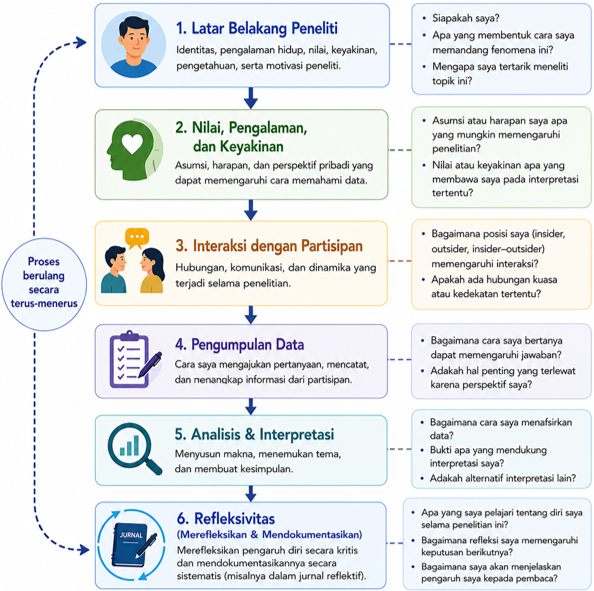
\includegraphics[keepaspectratio]{images/refleksivitas.png}}
\caption{Proses refleksivitas peneliti}
\end{figure}

}

\caption{\label{fig-refleksivitas}}

\end{figure}%

Gambar~\ref{fig-refleksivitas} menunjukkan bahwa refleksivitas merupakan
proses yang berlangsung secara berkesinambungan pada setiap tahap
penelitian. Pada setiap tahap tersebut, peneliti perlu mengajukan
pertanyaan reflektif yang berbeda, mulai dari menyadari motivasi memilih
topik penelitian, mengevaluasi hubungan dengan partisipan, hingga
menilai apakah interpretasi yang dihasilkan benar-benar didukung oleh
data. Dengan demikian, refleksivitas menjadi bagian yang tidak
terpisahkan dari seluruh proses penelitian kualitatif.

\subsection{\texorpdfstring{Jurnal Reflektif (\emph{Reflexive
Journal})}{Jurnal Reflektif (Reflexive Journal)}}\label{jurnal-reflektif-reflexive-journal}

Salah satu cara untuk menerapkan refleksivitas adalah dengan menyusun
\textbf{jurnal reflektif}, yaitu catatan yang dibuat secara berkala
selama penelitian untuk mendokumentasikan pemikiran, pengalaman,
keputusan metodologis, serta refleksi peneliti terhadap proses
penelitian. Berbeda dengan \emph{field notes} yang berfokus pada hasil
observasi atau wawancara, jurnal reflektif berisi evaluasi diri mengenai
bagaimana latar belakang, asumsi, maupun interaksi peneliti dapat
memengaruhi proses dan interpretasi penelitian (Olmos-Vega dkk., 2023;
Palaganas dkk., 2017).

Jurnal reflektif tidak memiliki format yang baku. Peneliti dapat
menyesuaikan bentuknya dengan kebutuhan penelitian, tetapi umumnya
memuat peristiwa yang terjadi, refleksi peneliti, dan tindak lanjut yang
akan dilakukan. Contoh jurnal reflektif disajikan pada Tabel 23.3.

\begin{longtable}[]{@{}
  >{\raggedright\arraybackslash}p{(\linewidth - 6\tabcolsep) * \real{0.2500}}
  >{\raggedright\arraybackslash}p{(\linewidth - 6\tabcolsep) * \real{0.2500}}
  >{\raggedright\arraybackslash}p{(\linewidth - 6\tabcolsep) * \real{0.2500}}
  >{\raggedright\arraybackslash}p{(\linewidth - 6\tabcolsep) * \real{0.2500}}@{}}
\caption{Contoh jurnal reflektif}\label{tbl-jurnal}\tabularnewline
\toprule\noalign{}
\endfirsthead
\endhead
\bottomrule\noalign{}
\endlastfoot
\textbf{Tahap Penelitian} & \textbf{Peristiwa} & \textbf{Refleksi
Peneliti} & \textbf{Tindak Lanjut} \\
Pengumpulan data & Wawancara pertama dengan mahasiswa tahun pertama
mengenai pengalaman beradaptasi di perguruan tinggi. & Saya adalah dosen
di fakultas yang sama sehingga beberapa partisipan tampak berhati-hati
ketika menyampaikan pengalaman negatif. Posisi saya sebagai dosen
mungkin memengaruhi keterbukaan mereka dalam menjawab pertanyaan. & Pada
wawancara berikutnya saya akan kembali menegaskan bahwa seluruh jawaban
bersifat rahasia, tidak memengaruhi penilaian akademik, dan partisipan
bebas menghentikan wawancara kapan saja. \\
Analisis data & Melakukan pengkodean (\emph{coding}) terhadap transkrip
wawancara. & Saya menyadari lebih mudah mengenali kutipan yang sesuai
dengan dugaan awal penelitian dibandingkan kutipan yang bertentangan.
Hal ini berpotensi menyebabkan saya mengabaikan informasi yang sama
pentingnya. & Meninjau kembali seluruh transkrip secara sistematis dan
mendiskusikan hasil pengkodean dengan dosen pembimbing untuk memperoleh
sudut pandang lain. \\
Penyusunan laporan & Menyusun hasil dan pembahasan penelitian. & Saya
perlu memastikan bahwa setiap tema didukung oleh kutipan partisipan yang
memadai, bukan hanya berdasarkan interpretasi pribadi. Saya juga perlu
menjelaskan posisi saya sebagai dosen agar pembaca memahami konteks
penelitian. & Menambahkan kutipan langsung yang mewakili setiap tema
serta menjelaskan \emph{positionality} peneliti pada bagian metode
penelitian. \\
\end{longtable}

Contoh pada Tabel~\ref{tbl-jurnal} menunjukkan bahwa jurnal reflektif
bukan sekadar catatan harian, melainkan sarana untuk mendokumentasikan
bagaimana peneliti mengenali dan mengelola pengaruh dirinya selama
penelitian berlangsung. Dengan melakukan refleksi secara berkelanjutan,
peneliti dapat meningkatkan transparansi proses penelitian sekaligus
memperkuat kepercayaan terhadap temuan yang dihasilkan.

\begin{tcolorbox}[enhanced jigsaw, colframe=quarto-callout-tip-color-frame, toptitle=1mm, breakable, leftrule=.75mm, arc=.35mm, toprule=.15mm, colback=white, colbacktitle=quarto-callout-tip-color!10!white, bottomtitle=1mm, bottomrule=.15mm, titlerule=0mm, title=\textcolor{quarto-callout-tip-color}{\faLightbulb}\hspace{0.5em}{Rangkuman}, coltitle=black, left=2mm, opacitybacktitle=0.6, opacityback=0, rightrule=.15mm]

\begin{enumerate}
\def\labelenumi{\arabic{enumi}.}
\tightlist
\item
  Penelitian kualitatif menggunakan konsep \emph{trustworthiness} untuk
  menilai kualitas proses dan temuan penelitian, yang mencakup empat
  kriteria utama: \emph{credibility, transferability, dependability},
  dan \emph{confirmability}.
\item
  Keempat kriteria \emph{trustworthiness} dapat ditingkatkan melalui
  berbagai strategi, seperti triangulasi, \emph{member checking},
  \emph{audit trail}, \emph{peer debriefing}, dan \emph{thick
  description}, sesuai dengan tujuan dan konteks penelitian.
\item
  Refleksivitas (\emph{reflexivity}) merupakan proses mengevaluasi
  secara kritis bagaimana latar belakang, pengalaman, nilai, dan posisi
  (\emph{positionality}) peneliti dapat memengaruhi proses maupun hasil
  penelitian.
\item
  Jurnal reflektif (\emph{reflexive journal}) merupakan salah satu cara
  untuk mendokumentasikan proses refleksi peneliti sehingga keputusan
  metodologis dan interpretasi data menjadi lebih transparan.
\item
  Penerapan \emph{trustworthiness} dan refleksivitas secara konsisten
  akan meningkatkan kredibilitas, transparansi, dan akuntabilitas
  penelitian kualitatif.
\end{enumerate}

\end{tcolorbox}

\begin{tcolorbox}[enhanced jigsaw, colframe=quarto-callout-important-color-frame, toptitle=1mm, breakable, leftrule=.75mm, arc=.35mm, toprule=.15mm, colback=white, colbacktitle=quarto-callout-important-color!10!white, bottomtitle=1mm, bottomrule=.15mm, titlerule=0mm, title=\textcolor{quarto-callout-important-color}{\faExclamation}\hspace{0.5em}{Refleksi \& Diskusi}, coltitle=black, left=2mm, opacitybacktitle=0.6, opacityback=0, rightrule=.15mm]

\begin{itemize}
\tightlist
\item
  Dari empat kriteria \emph{trustworthiness} (\emph{credibility,
  transferability, dependability}, dan \emph{confirmability}), menurut
  Anda manakah yang paling menantang untuk diterapkan dalam penelitian
  kualitatif? Berikan alasannya.
\item
  Bayangkan Anda akan melakukan penelitian kualitatif untuk skripsi.
  Strategi apa saja yang akan Anda gunakan untuk meningkatkan
  \emph{trustworthiness} penelitian tersebut? Jelaskan alasan
  pemilihannya.
\item
  Identifikasi \emph{positionality} Anda sebagai peneliti pada topik
  penelitian yang ingin Anda lakukan. Apakah Anda lebih berperan sebagai
  \emph{insider}, \emph{outsider}, atau berada di antara keduanya?
  Bagaimana posisi tersebut dapat memengaruhi proses penelitian?
\item
  Tuliskan satu contoh entri jurnal reflektif berdasarkan topik
  penelitian yang Anda rencanakan. Uraikan peristiwa yang dialami,
  refleksi yang muncul, serta tindak lanjut yang akan Anda lakukan untuk
  menjaga kualitas penelitian.
\end{itemize}

\end{tcolorbox}

\phantomsection\label{refs--20}
\begin{CSLReferences}{1}{0}
\bibitem[\citeproctext]{ref-Berger2015--20}
Berger, R. (2015). Now I see it, now I don't: researcher's position and
reflexivity in qualitative research. \emph{Qualitative Research},
\emph{15}, 219--234. \url{https://doi.org/10.1177/1468794112468475}

\bibitem[\citeproctext]{ref-Creswell2023--20}
Creswell, J. W., \& Poth, C. N. (2023). \emph{Qualitative inquiry \&
research design: Choosing among five approaches} (5th ed.). SAGE
Publications, Inc.

\bibitem[\citeproctext]{ref-Dodgson2019--20}
Dodgson, J. E. (2019). Reflexivity in Qualitative Research.
\emph{Journal of Human Lactation}, \emph{35}, 220--222.
\url{https://doi.org/10.1177/0890334419830990}

\bibitem[\citeproctext]{ref-Geertz1973--20}
Geertz, C. (1973). \emph{The interpretation of cultures: selected
essays} (hlm. 470). Basic Books.

\bibitem[\citeproctext]{ref-Lincoln1990--20}
Lincoln, Y. S., \& Guba, E. G. (1985). \emph{Naturalistic inquiry}.
Sage.

\bibitem[\citeproctext]{ref-Olmos-Vega2023--20}
Olmos-Vega, F. M., Stalmeijer, R. E., Varpio, L., \& Kahlke, R. (2023).
A practical guide to reflexivity in qualitative research: AMEE Guide No.
149. \emph{Medical Teacher}, \emph{45}, 241--251.
\url{https://doi.org/10.1080/0142159X.2022.2057287}

\bibitem[\citeproctext]{ref-Palaganas2017--20}
Palaganas, E., Sanchez, M., Molintas, Ma. V., \& Caricativo, R. (2017).
Reflexivity in Qualitative Research: A Journey of Learning. \emph{The
Qualitative Report}. \url{https://doi.org/10.46743/2160-3715/2017.2552}

\bibitem[\citeproctext]{ref-Patton2014--20}
Patton, M. Q. (2014). \emph{Qualitative research \& evaluation methods:
Integrating theory and practice}. SAGE Publications, Inc.

\bibitem[\citeproctext]{ref-Shenton2004--20}
Shenton, A. K. (2004). Strategies for ensuring trustworthiness in
qualitative research projects. \emph{Education for Information},
\emph{22}, 63--75.
\url{https://doi.org/10.3233/EFI-2004-22201;WGROUP:STRING:PUBLICATION}

\end{CSLReferences}

\chapter{Pelaporan Penelitian Kualitatif: Metode
COREQ}\label{pelaporan-penelitian-kualitatif-metode-coreq}

\begin{tcolorbox}[enhanced jigsaw, colframe=quarto-callout-note-color-frame, toptitle=1mm, breakable, leftrule=.75mm, arc=.35mm, toprule=.15mm, colback=white, colbacktitle=quarto-callout-note-color!10!white, bottomtitle=1mm, bottomrule=.15mm, titlerule=0mm, title=\textcolor{quarto-callout-note-color}{\faInfo}\hspace{0.5em}{Capaian Pembelajaran}, coltitle=black, left=2mm, opacitybacktitle=0.6, opacityback=0, rightrule=.15mm]

Setelah mempelajari bab ini, mahasiswa diharapkan mampu:

\begin{enumerate}
\def\labelenumi{\arabic{enumi}.}
\tightlist
\item
  Memahami definisi, urgensi, dan batasan ruang lingkup penggunaan
  panduan COREQ sebagai instrumen transparansi dalam pelaporan riset
  kualitatif berbasis wawancara dan FGD.
\item
  Mengimplementasikan panduan COREQ dalam pelaporan riset kualitatif.
\item
  Mengevaluasi kelengkapan laporan penelitian kualitatif berdasarkan
  butir-butir dalam panduan COREQ
\end{enumerate}

\end{tcolorbox}

Penelitian kualitatif tidak hanya menuntut penyajian temuan penelitian,
tetapi juga pelaporan yang transparan mengenai bagaimana data
dikumpulkan, dianalisis, dan diinterpretasikan. Transparansi ini penting
agar pembaca dapat menilai kredibilitas serta keterpercayaan temuan yang
dihasilkan. Oleh karena itu, berbagai panduan pelaporan (\emph{reporting
guidelines}) dikembangkan untuk membantu peneliti melaporkan penelitian
kualitatif secara lebih sistematis, lengkap, dan transparan. Salah satu
panduan yang paling banyak digunakan adalah \emph{Consolidated Criteria
for Reporting Qualitative Research} (COREQ).

\section{Latar Belakang Pengembangan Panduan
COREQ}\label{latar-belakang-pengembangan-panduan-coreq}

COREQ merupakan sebuah panduan pelaporan penelitian kualitatif yang
dikembangkan oleh~Tong dkk. (2007). Panduan ini memuat daftar periksa
yang terdiri atas 32 butir penilaian dengan tujuan untuk memastikan
peneliti melaporkan penelitian kualitatif secara lengkap dan transparan.
Melalui transparansi tersebut, COREQ diharapkan dapat meningkatkan
rigoritas, komprehensifitas, dan kredibilitas dari studi yang
bersangkutan (Barbieri dkk., 2025; Walsh dkk., 2020).

Ruang lingkup penggunaan COREQ terbatas pada penelitian kualitatif yang
menggunakan metode pengumpulan data wawancara dan diskusi kelompok
terfokus saja (Barbieri dkk., 2025; Tong dkk., 2007). Saat ini, COREQ
telah didukung secara luas oleh berbagai lembaga pelaporan ilmiah,
seperti EQUATOR Network, serta menjadi prasyarat atau rekomendasi di
banyak jurnal ilmiah bereputasi.

\section{Tujuan Penggunaan Panduan
COREQ}\label{tujuan-penggunaan-panduan-coreq}

Penggunaan panduan COREQ dalam pelaporan penelitian kualitatif memiliki
tujuan sebagai berikut:

\begin{enumerate}
\def\labelenumi{\alph{enumi}.}
\tightlist
\item
  Meningkatkan transparansi dan kelengkapan laporan penelitian. COREQ
  mengidentifikasi poin-poin penting yang wajib dilaporkan---seperti
  siapa yang melakukan penelitian, bagaimana penentuan sampel partisipan
  dilakukan, serta bagaimana data dikumpulkan dan dianalisis---agar
  pembaca dapat melakukan penilaian kritis terhadap metode dan temuan
  penelitian (Fehring dkk., 2025; Walsh dkk., 2020).
\item
  Mendukung rigoritas, kredibilitas, dan interpretabilitas penelitian
  kualitatif. Dengan mewajibkan rincian mengenai pemilihan partisipan,
  latar penelitian, pengumpulan data, dan proses analisis, COREQ
  membantu penelaah (\emph{reviewer}) dalam menilai ketepatan metodologi
  dan keabsahan temuan (Buus \& Perron, 2020; Harley \& Cornelissen,
  2022).
\item
  Menyelaraskan laporan dengan standar jurnal dan komunitas ilmiah.
  Sebagai salah satu alat pelaporan kualitatif yang paling banyak
  digunakan dan disitasi, COREQ telah diterima oleh jaringan akademik
  dan jurnal utama sebagai standar baku (Dossett dkk., 2021).
\end{enumerate}

\section{\texorpdfstring{Hubungan COREQ dengan \emph{Trustworthiness}
Penelitian
Kualitatif}{Hubungan COREQ dengan Trustworthiness Penelitian Kualitatif}}\label{hubungan-coreq-dengan-trustworthiness-penelitian-kualitatif}

Dalam penelitian kualitatif, kualitas penelitian umumnya dinilai melalui
konsep \emph{trustworthiness}, yang mencakup kredibilitas
(\emph{credibility}), keteralihan (\emph{transferability}), keandalan
(\emph{dependability}), dan kepastian (\emph{confirmability}). Keempat
aspek tersebut membantu pembaca menilai sejauh mana temuan penelitian
dapat dipercaya dan didukung oleh data yang memadai (Ahmed, 2024; Kakar
dkk., 2023).

Penting untuk dipahami bahwa COREQ bukanlah instrumen untuk mengukur
\emph{trustworthiness} secara langsung. COREQ merupakan panduan
pelaporan yang membantu peneliti menyajikan informasi penting secara
lengkap dan transparan, sehingga pembaca dapat menilai sendiri kualitas
penelitian yang dilakukan.

Dengan kata lain, COREQ tidak menjamin bahwa suatu penelitian
berkualitas tinggi, tetapi membantu memastikan bahwa informasi yang
diperlukan untuk menilai kualitas tersebut tersedia secara memadai. Oleh
karena itu, COREQ sebaiknya dipandang sebagai alat untuk meningkatkan
transparansi pelaporan penelitian kualitatif, bukan sebagai satu-satunya
tolok ukur kualitas penelitian (Fehring dkk., 2025).

\section{Ranah (Domain) dalam COREQ}\label{ranah-domain-dalam-coreq}

Terdapat tiga ranah dalam COREQ yakni ranah tim peneliti dan
refleksivitas, ranah desain dan metode penelitian, serta ranah analisis
dan penyajian hasil penelitian. Untuk memudahkan pemahaman,
Tabel~\ref{tbl-domaincoreq} menyajikan ringkasan struktur 32 butir
pelaporan dalam panduan COREQ. Ketiga ranah tersebut mencakup aspek
peneliti, desain penelitian, serta analisis dan pelaporan temuan yang
secara keseluruhan bertujuan meningkatkan transparansi penelitian
kualitatif. Lihat \hyperref[sec-coreq]{Lampiran} untuk mempelajari
struktur COREQ \emph{Checklist} secara lengkap.

\begin{longtable}[]{@{}
  >{\raggedright\arraybackslash}p{(\linewidth - 6\tabcolsep) * \real{0.2500}}
  >{\raggedright\arraybackslash}p{(\linewidth - 6\tabcolsep) * \real{0.2500}}
  >{\raggedright\arraybackslash}p{(\linewidth - 6\tabcolsep) * \real{0.2500}}
  >{\raggedright\arraybackslash}p{(\linewidth - 6\tabcolsep) * \real{0.2500}}@{}}
\caption{Struktur COREQ}\label{tbl-domaincoreq}\tabularnewline
\toprule\noalign{}
\begin{minipage}[b]{\linewidth}\raggedright
Ranah
\end{minipage} & \begin{minipage}[b]{\linewidth}\raggedright
Subranah
\end{minipage} & \begin{minipage}[b]{\linewidth}\raggedright
Nomor Item COREQ
\end{minipage} & \begin{minipage}[b]{\linewidth}\raggedright
Jumlah Item
\end{minipage} \\
\midrule\noalign{}
\endfirsthead
\toprule\noalign{}
\begin{minipage}[b]{\linewidth}\raggedright
Ranah
\end{minipage} & \begin{minipage}[b]{\linewidth}\raggedright
Subranah
\end{minipage} & \begin{minipage}[b]{\linewidth}\raggedright
Nomor Item COREQ
\end{minipage} & \begin{minipage}[b]{\linewidth}\raggedright
Jumlah Item
\end{minipage} \\
\midrule\noalign{}
\endhead
\bottomrule\noalign{}
\endlastfoot
Tim Peneliti dan Refleksivitas & Karakteristik personal; hubungan dengan
partisipan & 1--8 & 8 \\
Desain Penelitian & Kerangka teoretis; pemilihan partisipan; setting;
pengumpulan data & 9--23 & 15 \\
Analisis dan Temuan & Analisis data; pelaporan hasil & 24--32 & 9 \\
\textbf{Total} & & & \textbf{32} \\
\end{longtable}

\subsection{Ranah Tim Peneliti dan
Refleksivitas}\label{ranah-tim-peneliti-dan-refleksivitas}

Ranah ini berfokus pada karakteristik peneliti serta hubungan antara
peneliti dan partisipan yang berpotensi memengaruhi proses penelitian.
Aspek yang dilaporkan meliputi identitas dan latar belakang pewawancara
atau fasilitator, pengalaman dan pelatihan yang dimiliki, serta hubungan
yang telah terjalin dengan partisipan sebelum penelitian dilakukan.
Selain itu, COREQ juga menekankan pentingnya melaporkan informasi yang
diketahui partisipan tentang peneliti dan berbagai faktor yang dapat
memengaruhi interaksi selama proses pengumpulan data.

Pelaporan aspek-aspek tersebut penting karena dalam penelitian
kualitatif, peneliti merupakan bagian dari proses produksi data.
Karakteristik, pengalaman, asumsi, dan posisi sosial peneliti dapat
memengaruhi cara data dikumpulkan, dianalisis, dan diinterpretasikan.
Oleh karena itu, transparansi mengenai tim peneliti dan praktik
refleksivitas membantu pembaca memahami konteks di balik temuan
penelitian serta menilai potensi pengaruh yang mungkin muncul selama
proses penelitian. (Mason-Bish, 2019; Zayhowski dkk., 2025).

\emph{Contoh Pelaporan Tim Peneliti dan Refleksivitas}

\textbf{Kurang lengkap}

\begin{quote}
Wawancara dilakukan oleh peneliti.
\end{quote}

\textbf{Lebih sesuai dengan COREQ}

\begin{quote}
Wawancara dilakukan oleh penulis pertama (perempuan, dosen psikologi
dengan gelar doktor, memiliki pengalaman lima tahun dalam penelitian
kualitatif dan telah mengikuti pelatihan wawancara mendalam). Sebelum
penelitian dimulai, peneliti belum memiliki hubungan pribadi dengan
partisipan.
\end{quote}

\subsection{Ranah Desain dan Metode
Penelitian}\label{ranah-desain-dan-metode-penelitian}

Ranah ini menjelaskan bagaimana penelitian dirancang dan dilaksanakan.
Informasi yang perlu dilaporkan mencakup orientasi metodologis atau
kerangka teoretis yang digunakan, strategi pemilihan partisipan, proses
rekrutmen, karakteristik dan jumlah partisipan, serta latar penelitian.
Selain itu, ranah ini juga mencakup prosedur pengumpulan data, seperti
penggunaan panduan wawancara, durasi wawancara atau FGD, perekaman data,
catatan lapangan, saturasi data, dan konfirmasi hasil kepada partisipan.

Pelaporan yang jelas mengenai desain dan metode penelitian memungkinkan
pembaca menilai kesesuaian antara pertanyaan penelitian, metode yang
digunakan, dan temuan yang dihasilkan. Transparansi pada aspek ini juga
membantu pembaca memahami konteks penelitian, menilai keterpercayaan
proses pengumpulan data, serta mengevaluasi relevansi temuan untuk
konteks lain yang serupa (Dossett dkk., 2021; Harley \& Cornelissen,
2022).

\emph{Contoh Pelaporan Desain dan Metode Penelitian}

\textbf{Kurang lengkap}

\begin{quote}
Penelitian melibatkan beberapa mahasiswa dan menggunakan wawancara
mendalam.
\end{quote}

\textbf{Lebih sesuai dengan COREQ}

\begin{quote}
Partisipan dipilih menggunakan teknik \emph{purposive sampling} dengan
kriteria mahasiswa aktif semester 6--8 yang pernah mengikuti program
magang minimal satu semester. Sebanyak 15 partisipan direkrut melalui
pengumuman daring. Wawancara berlangsung selama 45--60 menit dan direkam
menggunakan perangkat audio digital.
\end{quote}

\subsection{Ranah Analisis dan Penyajian Temuan
Penelitian}\label{ranah-analisis-dan-penyajian-temuan-penelitian}

Ranah ini berfokus pada bagaimana data dianalisis dan bagaimana hasil
penelitian dilaporkan. Pada tahap analisis, peneliti perlu menjelaskan
proses pengodean data, jumlah analis atau coder yang terlibat, cara
pengembangan tema, serta penggunaan perangkat lunak analisis data
kualitatif jika digunakan. Pada tahap pelaporan hasil, peneliti perlu
menyajikan tema-tema yang ditemukan, kutipan partisipan yang mendukung
interpretasi, serta hubungan yang jelas antara data dan kesimpulan yang
dibuat.

Pelaporan yang transparan mengenai proses analisis dan penyajian temuan
membantu pembaca menilai kredibilitas interpretasi yang dihasilkan.
Dengan mengetahui bagaimana tema dibangun dan bagaimana data mendukung
temuan penelitian, pembaca dapat mengevaluasi keterpercayaan hasil
penelitian secara lebih objektif (Ahmed, 2024; Kakar dkk., 2023).

\emph{Contoh Pelaporan Analisis dan Temuan}

\textbf{Kurang lengkap}

\begin{quote}
Dari hasil wawancara ditemukan beberapa tema utama.
\end{quote}

\textbf{Lebih sesuai dengan COREQ}

\begin{quote}
Analisis tematik menghasilkan tiga tema utama, yaitu (1) ketidakpastian
karier, (2) dukungan sosial sebagai sumber resiliensi, dan (3) strategi
adaptasi terhadap tekanan akademik. Tema-tema tersebut dikembangkan
melalui proses pengodean induktif yang dilakukan oleh dua peneliti
secara independen menggunakan NVivo 14. Salah satu kutipan yang
mendukung tema kedua adalah: ``Teman-teman saya menjadi tempat utama
untuk berbagi ketika menghadapi kesulitan akademik'' (P07).
\end{quote}

\section{Keterbatasan Panduan COREQ}\label{keterbatasan-panduan-coreq}

Meskipun banyak digunakan dalam pelaporan penelitian kualitatif, panduan
COREQ memiliki beberapa keterbatasan yang perlu dipahami oleh peneliti.

\begin{enumerate}
\def\labelenumi{\arabic{enumi}.}
\item
  Panduan COREQ dirancang terutama untuk penelitian kualitatif yang
  menggunakan wawancara dan diskusi kelompok terfokus (FGD), sehingga
  tidak selalu sesuai untuk metode pengumpulan data lain, seperti
  observasi partisipan, etnografi, autoetnografi, atau penelitian
  berbasis seni (\emph{arts-based research}) (Barbieri dkk., 2025; Braun
  \& Clarke, 2025).
\item
  COREQ merupakan panduan pelaporan (\emph{reporting guideline}), bukan
  instrumen untuk menilai kualitas metodologis penelitian. Suatu
  penelitian dapat memenuhi seluruh butir COREQ, tetapi tetap memiliki
  kelemahan dalam perumusan masalah, pengumpulan data, analisis, maupun
  interpretasi hasil (Buus \& Perron, 2020).
\item
  Penggunaan COREQ secara terlalu kaku berpotensi menimbulkan fenomena
  \emph{overobedience}, yaitu ketika peneliti lebih berfokus pada
  pemenuhan daftar periksa dibandingkan pada kualitas substansi
  penelitian yang dilakukan. Akibatnya, laporan penelitian dapat tampak
  lengkap secara formal, tetapi kurang mencerminkan kedalaman analisis
  yang menjadi ciri utama penelitian kualitatif (Barbieri dkk., 2025;
  Buus \& Perron, 2020).
\end{enumerate}

Oleh karena itu, COREQ sebaiknya digunakan sebagai panduan untuk
meningkatkan transparansi pelaporan penelitian, bukan sebagai
satu-satunya tolok ukur kualitas penelitian kualitatif. Penilaian
kualitas penelitian tetap harus mempertimbangkan kesesuaian metodologi,
kedalaman analisis, serta tingkat keterpercayaan
(\emph{trustworthiness}) temuan yang dihasilkan.

\begin{tcolorbox}[enhanced jigsaw, colframe=quarto-callout-tip-color-frame, toptitle=1mm, breakable, leftrule=.75mm, arc=.35mm, toprule=.15mm, colback=white, colbacktitle=quarto-callout-tip-color!10!white, bottomtitle=1mm, bottomrule=.15mm, titlerule=0mm, title=\textcolor{quarto-callout-tip-color}{\faLightbulb}\hspace{0.5em}{Rangkuman}, coltitle=black, left=2mm, opacitybacktitle=0.6, opacityback=0, rightrule=.15mm]

\begin{enumerate}
\def\labelenumi{\arabic{enumi}.}
\tightlist
\item
  COREQ (\emph{Consolidated Criteria for Reporting Qualitative
  Research}) merupakan panduan pelaporan penelitian kualitatif yang
  terdiri atas 32 butir pelaporan untuk membantu peneliti menyajikan
  penelitian secara lengkap, sistematis, dan transparan. guna
  meningkatkan rigoritas, kelengkapan, dan kredibilitas studi.
\item
  COREQ dirancang terutama untuk penelitian kualitatif yang menggunakan
  metode wawancara dan diskusi kelompok terfokus (\emph{focus group
  discussion}).
\item
  Melalui pelaporan yang transparan, COREQ membantu pembaca menilai
  keterpercayaan (\emph{trustworthiness}) penelitian, termasuk
  kredibilitas, keandalan, keteralihan, dan kepastian temuan.
\item
  COREQ mengelompokkan 32 butir pelaporannya ke dalam tiga ranah utama,
  yaitu tim peneliti dan refleksivitas, desain dan metode penelitian,
  serta analisis dan penyajian temuan penelitian.
\item
  COREQ merupakan panduan pelaporan, bukan instrumen penilaian kualitas
  penelitian. Oleh karena itu, penggunaan COREQ perlu disertai
  pertimbangan metodologis lain dan tidak dijadikan satu-satunya tolok
  ukur kualitas penelitian kualitatif.
\end{enumerate}

\end{tcolorbox}

\begin{tcolorbox}[enhanced jigsaw, colframe=quarto-callout-important-color-frame, toptitle=1mm, breakable, leftrule=.75mm, arc=.35mm, toprule=.15mm, colback=white, colbacktitle=quarto-callout-important-color!10!white, bottomtitle=1mm, bottomrule=.15mm, titlerule=0mm, title=\textcolor{quarto-callout-important-color}{\faExclamation}\hspace{0.5em}{Refleksi \& Diskusi}, coltitle=black, left=2mm, opacitybacktitle=0.6, opacityback=0, rightrule=.15mm]

\begin{itemize}
\tightlist
\item
  Dalam penelitian kuantitatif, kualitas riset diuji dengan angka-angka
  statistik (seperti uji validitas dan reliabilitas). Karena penelitian
  kualitatif tidak menggunakan angka, bagaimana cara kita meyakinkan
  pembaca bahwa hasil wawancara kita itu jujur, ilmiah, dan bisa
  dipercaya? Di mana peran COREQ dalam menjembatani hal ini?
\item
  Pilihlah satu artikel penelitian kualitatif berbasis wawancara atau
  FGD. Jika Anda diminta menjadi reviewer, apakah laporan penelitian
  tersebut sudah memenuhi prinsip-prinsip COREQ? Jelaskan aspek apa saja
  yang telah dilaporkan dengan baik dan aspek apa saja yang masih perlu
  diperbaiki.
\item
  Bayangkan Anda sedang mereview sebuah draf skripsi. Secara formalitas,
  mahasiswa tersebut mencentang semua dari 32 butir di COREQ. Namun,
  setelah dibaca, analisisnya sangat dangkal dan tidak menjawab
  pertanyaan penelitian. Apakah skripsi tersebut bisa dikatakan
  berkualitas tinggi hanya karena skor COREQ-nya sempurna? Berikan
  alasannya.
\end{itemize}

\end{tcolorbox}

\phantomsection\label{refs--21}
\begin{CSLReferences}{1}{0}
\bibitem[\citeproctext]{ref-Ahmed2024--21}
Ahmed, S. K. (2024). The pillars of trustworthiness in qualitative
research. \emph{Journal of Medicine, Surgery, and Public Health},
\emph{2}, 100051. \url{https://doi.org/10.1016/J.GLMEDI.2024.100051}

\bibitem[\citeproctext]{ref-Barbieri2025--21}
Barbieri, M., Moro, A., Gammone, M., Cattani, D., Delbene, L., Sallai,
T., Watson, R., Catania, G., Zanini, M., Sasso, L., \& Bagnasco, A.
(2025). Reporting Grounded Theory: Is COREQ Enough? \emph{Journal of
clinical nursing}, \emph{34}, 3439--3441.
\url{https://doi.org/10.1111/JOCN.70052}

\bibitem[\citeproctext]{ref-Braun2025--21}
Braun, V., \& Clarke, V. (2025). Reporting guidelines for qualitative
research: a values-based approach. \emph{Qualitative Research in
Psychology}, \emph{22}, 399--438.
\url{https://doi.org/10.1080/14780887.2024.2382244}

\bibitem[\citeproctext]{ref-Buus2020--21}
Buus, N., \& Perron, A. (2020). The quality of quality criteria:
Replicating the development of the Consolidated Criteria for Reporting
Qualitative Research (COREQ). \emph{International Journal of Nursing
Studies}, \emph{102}, 103452.
\url{https://doi.org/10.1016/J.IJNURSTU.2019.103452}

\bibitem[\citeproctext]{ref-Dossett2021--21}
Dossett, L. A., Kaji, A. H., \& Cochran, A. (2021). SRQR and COREQ
Reporting Guidelines for Qualitative Studies. \emph{JAMA Surgery},
\emph{156}, 875--876. \url{https://doi.org/10.1001/jamasurg.2021.0525}

\bibitem[\citeproctext]{ref-Fehring2025--21}
Fehring, L., Frings, J., Rust, P., Kempny, C., Thürmann, P. A., \&
Meister, S. (2025). Extension of the Consolidated Criteria for Reporting
Qualitative Research Guideline to Large Language Models (COREQ+LLM):
Protocol for a Multiphase Study. \emph{JMIR research protocols},
\emph{14}, e78682. \url{https://doi.org/10.2196/78682}

\bibitem[\citeproctext]{ref-Harley2022--21}
Harley, B., \& Cornelissen, J. (2022). Rigor With or Without Templates?
The Pursuit of Methodological Rigor in Qualitative Research.
\emph{Organizational Research Methods}, \emph{25}, 239--261.
\url{https://doi.org/10.1177/1094428120937786}

\bibitem[\citeproctext]{ref-Kakar2023--21}
Kakar, Z. U. H., Rasheed, R., Rashid, A., Akhter, S., Kakar, Z. U. H.,
Rasheed, R., Rashid, A., \& Akhter, S. (2023). Criteria for Assessing
and Ensuring the Trustworthiness in Qualitative Research.
\emph{Publications and Research}.
\url{https://academicworks.cuny.edu/yc_pubs/342}

\bibitem[\citeproctext]{ref-Mason-Bish2019--21}
Mason-Bish, H. (2019). The elite delusion: reflexivity, identity and
positionality in qualitative research. \emph{Qualitative Research},
\emph{19}, 263--276. \url{https://doi.org/10.1177/1468794118770078}

\bibitem[\citeproctext]{ref-Tong2007--21}
Tong, A., Sainsbury, P., \& Craig, J. (2007). Consolidated criteria for
reporting qualitative research (COREQ): a 32-item checklist for
interviews and focus groups. \emph{International Journal for Quality in
Health Care}, \emph{19}, 349--357.
\url{https://doi.org/10.1093/intqhc/mzm042}

\bibitem[\citeproctext]{ref-Walsh2020--21}
Walsh, S., Jones, M., Bressington, D., McKenna, L., Brown, E., Terhaag,
S., Shrestha, M., Al-Ghareeb, A., \& Gray, R. (2020). Adherence to COREQ
Reporting Guidelines for Qualitative Research: A Scientometric Study in
Nursing Social Science. \emph{International Journal of Qualitative
Methods}, \emph{19}.
\url{https://doi.org/10.1177/1609406920982145;WGROUP:STRING:PUBLICATION}

\bibitem[\citeproctext]{ref-Zayhowski2025--21}
Zayhowski, K., Borle, K., \& Channaoui, N. (2025). Enhancing rigor and
justice in genetic counseling research with reflexivity and
positionality. \emph{Journal of Genetic Counseling}, \emph{34}, e70066.
\url{https://doi.org/10.1002/JGC4.70066;WGROUP:STRING:PUBLICATION}

\end{CSLReferences}

\section*{Lampiran}\label{sec-coreq}
\addcontentsline{toc}{section}{Lampiran}

\markright{Lampiran}

\begin{tcolorbox}[enhanced jigsaw, colframe=quarto-callout-note-color-frame, toptitle=1mm, breakable, leftrule=.75mm, arc=.35mm, toprule=.15mm, colback=white, colbacktitle=quarto-callout-note-color!10!white, bottomtitle=1mm, bottomrule=.15mm, titlerule=0mm, title={COREQ (COnsolidated criteria for REporting Qualitative research)
\emph{Checklist}}, coltitle=black, left=2mm, opacitybacktitle=0.6, opacityback=0, rightrule=.15mm]

\textbf{Ranah 1: Tim Peneliti dan Refleksi Diri}

a) Karakteristik Peneliti

\begin{longtable}[]{@{}
  >{\raggedright\arraybackslash}p{(\linewidth - 6\tabcolsep) * \real{0.2500}}
  >{\raggedright\arraybackslash}p{(\linewidth - 6\tabcolsep) * \real{0.2500}}
  >{\raggedright\arraybackslash}p{(\linewidth - 6\tabcolsep) * \real{0.2500}}
  >{\raggedright\arraybackslash}p{(\linewidth - 6\tabcolsep) * \real{0.2500}}@{}}
\toprule\noalign{}
\begin{minipage}[b]{\linewidth}\raggedright
Topik
\end{minipage} & \begin{minipage}[b]{\linewidth}\raggedright
No.~Item
\end{minipage} & \begin{minipage}[b]{\linewidth}\raggedright
Pertanyaan/Deskripsi Panduan
\end{minipage} & \begin{minipage}[b]{\linewidth}\raggedright
Dilaporkan di Halaman
\end{minipage} \\
\midrule\noalign{}
\endhead
\bottomrule\noalign{}
\endlastfoot
Pewawancara/ fasilitator & 1 & Siapa saja yang melakukan wawancara, FGD,
atau observasi dalam penelitian ini? & \\
Kredensial & 2 & Apa kredensial peneliti? & \\
Pekerjaan & 3 & Apa pekerjaan peneliti saat penelitian dilakukan? & \\
Gender & 4 & Apa gender peneliti? & \\
Pengalaman dan pelatihan & 5 & Apa pengalaman dan pelatihan yang telah
diperoleh peneliti terkait topik penelitian atau metode riset? & \\
\end{longtable}

b) Hubungan antara Peneliti dan Partisipan

\begin{longtable}[]{@{}
  >{\raggedright\arraybackslash}p{(\linewidth - 6\tabcolsep) * \real{0.2500}}
  >{\raggedright\arraybackslash}p{(\linewidth - 6\tabcolsep) * \real{0.2500}}
  >{\raggedright\arraybackslash}p{(\linewidth - 6\tabcolsep) * \real{0.2500}}
  >{\raggedright\arraybackslash}p{(\linewidth - 6\tabcolsep) * \real{0.2500}}@{}}
\toprule\noalign{}
\begin{minipage}[b]{\linewidth}\raggedright
Topik
\end{minipage} & \begin{minipage}[b]{\linewidth}\raggedright
No.~Item
\end{minipage} & \begin{minipage}[b]{\linewidth}\raggedright
Pertanyaan/Deskripsi Panduan
\end{minipage} & \begin{minipage}[b]{\linewidth}\raggedright
Dilaporkan di Halaman
\end{minipage} \\
\midrule\noalign{}
\endhead
\bottomrule\noalign{}
\endlastfoot
Hubungan yang terjalin & 6 & Apakah ada hubungan yang terjalin antara
peneliti dan partisipan sebelum dilakukannya penelitian? & \\
Pengetahuan partisipan tentang peneliti & 7 & Apa yang partisipan
ketahui tentang peneliti? Misalnya tujuan pribadi atau alasan
dilakukannya penelitian. & \\
Karakteristik pewawancara & 8 & Karakteristik apa yang dilaporkan
partisipan tentang pewawancara? Misalnya bias, asumsi, alasan, dan minat
terhadap topik penelitian. & \\
\end{longtable}

\textbf{Ranah 2: Desain Penelitian}

a) Kerangka Teoretis

\begin{longtable}[]{@{}
  >{\raggedright\arraybackslash}p{(\linewidth - 6\tabcolsep) * \real{0.2500}}
  >{\raggedright\arraybackslash}p{(\linewidth - 6\tabcolsep) * \real{0.2500}}
  >{\raggedright\arraybackslash}p{(\linewidth - 6\tabcolsep) * \real{0.2500}}
  >{\raggedright\arraybackslash}p{(\linewidth - 6\tabcolsep) * \real{0.2500}}@{}}
\toprule\noalign{}
\begin{minipage}[b]{\linewidth}\raggedright
Topik
\end{minipage} & \begin{minipage}[b]{\linewidth}\raggedright
No.~Item
\end{minipage} & \begin{minipage}[b]{\linewidth}\raggedright
Pertanyaan/Deskripsi Panduan
\end{minipage} & \begin{minipage}[b]{\linewidth}\raggedright
Dilaporkan di Halaman
\end{minipage} \\
\midrule\noalign{}
\endhead
\bottomrule\noalign{}
\endlastfoot
Orientasi metodologis dan teori & 9 & Apa kerangka teoritis atau desain
yang memayungi penelitian? Misalnya \emph{grounded theory},
fenomenologi, etnografi, dan sebagainya. & \\
\end{longtable}

b) Pemilihan Partisipan

\begin{longtable}[]{@{}
  >{\raggedright\arraybackslash}p{(\linewidth - 6\tabcolsep) * \real{0.2500}}
  >{\raggedright\arraybackslash}p{(\linewidth - 6\tabcolsep) * \real{0.2500}}
  >{\raggedright\arraybackslash}p{(\linewidth - 6\tabcolsep) * \real{0.2500}}
  >{\raggedright\arraybackslash}p{(\linewidth - 6\tabcolsep) * \real{0.2500}}@{}}
\toprule\noalign{}
\begin{minipage}[b]{\linewidth}\raggedright
Topik
\end{minipage} & \begin{minipage}[b]{\linewidth}\raggedright
No.~Item
\end{minipage} & \begin{minipage}[b]{\linewidth}\raggedright
Pertanyaan/Deskripsi Panduan
\end{minipage} & \begin{minipage}[b]{\linewidth}\raggedright
Dilaporkan di Halaman
\end{minipage} \\
\midrule\noalign{}
\endhead
\bottomrule\noalign{}
\endlastfoot
Teknik sampling & 10 & Bagaimana teknik sampling yang digunakan untuk
memilih partisipan penelitian? & \\
Metode pendekatan & 11 & Bagaimana peneliti melakukan pendekatan kepada
partisipan? Misalnya tatap muka, telepon, atau email. & \\
Jumlah sampel & 12 & Berapa jumlah partisipan dalam penelitian? & \\
Non-partisipan & 13 & Berapa orang yang menolak menjadi partisipan atau
dikeluarkan dari analisis? Apa alasannya? & \\
\end{longtable}

c) \emph{Setting}

\begin{longtable}[]{@{}
  >{\raggedright\arraybackslash}p{(\linewidth - 6\tabcolsep) * \real{0.2500}}
  >{\raggedright\arraybackslash}p{(\linewidth - 6\tabcolsep) * \real{0.2500}}
  >{\raggedright\arraybackslash}p{(\linewidth - 6\tabcolsep) * \real{0.2500}}
  >{\raggedright\arraybackslash}p{(\linewidth - 6\tabcolsep) * \real{0.2500}}@{}}
\toprule\noalign{}
\begin{minipage}[b]{\linewidth}\raggedright
Topik
\end{minipage} & \begin{minipage}[b]{\linewidth}\raggedright
No.~Item
\end{minipage} & \begin{minipage}[b]{\linewidth}\raggedright
Pertanyaan/Deskripsi Panduan
\end{minipage} & \begin{minipage}[b]{\linewidth}\raggedright
Dilaporkan di Halaman
\end{minipage} \\
\midrule\noalign{}
\endhead
\bottomrule\noalign{}
\endlastfoot
Setting pengumpulan data & 14 & Di mana pengambilan data dilakukan?
Misalnya rumah, kantor, atau kampus. & \\
Kehadiran non-partisipan & 15 & Apakah ada orang lain yang hadir selain
partisipan dan peneliti? & \\
Gambaran partisipan & 16 & Apa karakteristik penting dari partisipan?
Misalnya data demografis atau informasi relevan lainnya. & \\
\end{longtable}

d) Pengumpulan Data

\begin{longtable}[]{@{}
  >{\raggedright\arraybackslash}p{(\linewidth - 6\tabcolsep) * \real{0.2500}}
  >{\raggedright\arraybackslash}p{(\linewidth - 6\tabcolsep) * \real{0.2500}}
  >{\raggedright\arraybackslash}p{(\linewidth - 6\tabcolsep) * \real{0.2500}}
  >{\raggedright\arraybackslash}p{(\linewidth - 6\tabcolsep) * \real{0.2500}}@{}}
\toprule\noalign{}
\begin{minipage}[b]{\linewidth}\raggedright
Topik
\end{minipage} & \begin{minipage}[b]{\linewidth}\raggedright
No.~Item
\end{minipage} & \begin{minipage}[b]{\linewidth}\raggedright
Pertanyaan/Deskripsi Panduan
\end{minipage} & \begin{minipage}[b]{\linewidth}\raggedright
Dilaporkan di Halaman
\end{minipage} \\
\midrule\noalign{}
\endhead
\bottomrule\noalign{}
\endlastfoot
Panduan wawancara & 17 & Apakah pertanyaan, petunjuk, dan panduan
disediakan oleh peneliti? Apakah sudah diujicobakan? & \\
Wawancara berulang & 18 & Apakah dilakukan wawancara berulang? Jika ya,
berapa kali? & \\
Perekaman audio/video & 19 & Apakah peneliti menggunakan perekaman audio
atau video dalam pengambilan data? & \\
Catatan lapangan & 20 & Apakah peneliti membuat catatan lapangan selama
dan/atau setelah pengambilan data? & \\
Durasi wawancara & 21 & Berapa lama durasi wawancara? & \\
Saturasi data & 22 & Apakah saturasi data didiskusikan? & \\
Pengembalian transkrip wawancara & 23 & Apakah transkrip wawancara
dikembalikan kepada partisipan untuk meminta komentar dan/atau koreksi?
& \\
\end{longtable}

\textbf{Ranah 3: Analisis dan Temuan Penelitian}

a) Analisis Data

\begin{longtable}[]{@{}
  >{\raggedright\arraybackslash}p{(\linewidth - 6\tabcolsep) * \real{0.2500}}
  >{\raggedright\arraybackslash}p{(\linewidth - 6\tabcolsep) * \real{0.2500}}
  >{\raggedright\arraybackslash}p{(\linewidth - 6\tabcolsep) * \real{0.2500}}
  >{\raggedright\arraybackslash}p{(\linewidth - 6\tabcolsep) * \real{0.2500}}@{}}
\toprule\noalign{}
\begin{minipage}[b]{\linewidth}\raggedright
Topik
\end{minipage} & \begin{minipage}[b]{\linewidth}\raggedright
No.~Item
\end{minipage} & \begin{minipage}[b]{\linewidth}\raggedright
Pertanyaan/Deskripsi Panduan
\end{minipage} & \begin{minipage}[b]{\linewidth}\raggedright
Dilaporkan di Halaman
\end{minipage} \\
\midrule\noalign{}
\endhead
\bottomrule\noalign{}
\endlastfoot
Jumlah pengode data & 24 & Berapa orang yang terlibat dalam pemberian
kode data? & \\
Deskripsi \emph{coding tree} & 25 & Apakah peneliti memberikan deskripsi
mengenai \emph{coding tree}? & \\
Turunan tema & 26 & Apakah tema-tema telah diidentifikasi sejak awal
atau diturunkan dari data? & \\
Perangkat lunak & 27 & Apa perangkat lunak yang digunakan untuk mengolah
data? & \\
Pemeriksaan partisipan (\emph{member checking}) & 28 & Apakah partisipan
memberikan umpan balik terhadap temuan penelitian? & \\
\end{longtable}

b) Pelaporan

\begin{longtable}[]{@{}
  >{\raggedright\arraybackslash}p{(\linewidth - 6\tabcolsep) * \real{0.2500}}
  >{\raggedright\arraybackslash}p{(\linewidth - 6\tabcolsep) * \real{0.2500}}
  >{\raggedright\arraybackslash}p{(\linewidth - 6\tabcolsep) * \real{0.2500}}
  >{\raggedright\arraybackslash}p{(\linewidth - 6\tabcolsep) * \real{0.2500}}@{}}
\toprule\noalign{}
\begin{minipage}[b]{\linewidth}\raggedright
Topik
\end{minipage} & \begin{minipage}[b]{\linewidth}\raggedright
No.~Item
\end{minipage} & \begin{minipage}[b]{\linewidth}\raggedright
Pertanyaan/Deskripsi Panduan
\end{minipage} & \begin{minipage}[b]{\linewidth}\raggedright
Dilaporkan di Halaman
\end{minipage} \\
\midrule\noalign{}
\endhead
\bottomrule\noalign{}
\endlastfoot
Pemaparan kutipan & 29 & Apakah kutipan partisipan dipaparkan untuk
mengilustrasikan tema atau temuan penelitian? Apakah setiap kutipan
diidentifikasi (misalnya nomor partisipan)? & \\
Data dan temuan konsisten & 30 & Apakah terdapat konsistensi antara data
yang dipaparkan dengan temuan penelitian? & \\
Kejelasan tema-tema mayor & 31 & Apakah tema-tema mayor secara jelas
dipaparkan dalam temuan penelitian? & \\
Kejelasan tema-tema minor & 32 & Apakah terdapat deskripsi tentang
kasus-kasus yang berbeda atau pembahasan mengenai tema-tema minor? & \\
\end{longtable}

\end{tcolorbox}




\end{document}
